%\documentstyle[11pt,epsfig]{book}
\documentclass[11pt,a4paper]{book}
\usepackage{epsfig}
\usepackage{xcolor}
\usepackage[colorlinks=true,urlcolor=blue]{hyperref}
\hypersetup{pdfborder = {0 0 0}}
\usepackage{natbib}
\usepackage{multicol,multirow,array}
\usepackage{makeidx}
\usepackage{html}
\usepackage[utf8]{inputenc}
\usepackage[T1]{fontenc}
\usepackage{gensymb} %For the \degree symbol
\usepackage{longtable} %For tables spanned on multiple pages
%
%\date{February 20, 2009}
\setlength{\textwidth}{16.0cm}
\setlength{\textheight}{23.0cm}
\hoffset=-1.5cm
%\hoffset=-3cm
%\voffset=-3.2cm
\oddsidemargin=2cm
\evensidemargin=1cm
\renewcommand{\textfraction}{.15}
\renewcommand{\topfraction}{.85}
\renewcommand{\floatpagefraction}{.80}
\newcommand{\beq}{\begin{equation}}
\newcommand{\eeq}{\end{equation}}
\newcommand{\bull}{\vrule height .9ex width .8ex depth -.1ex \ }
%



\newcommand{\parttoccolor}{blue}
\newcommand{\chaptertoccolor}{blue}
\newcommand{\sectiontoccolor}{green!70!black}
\newcommand{\subsectiontoccolor}{violet}

\makeatletter
\renewcommand*\l@part[2]{%
  \ifnum \c@tocdepth >-2\relax
    \addpenalty{-\@highpenalty}%
    \addvspace{2.25em \@plus\p@}%
    \setlength\@tempdima{3em}%
    \begingroup
      \parindent \z@ \rightskip \@pnumwidth
      \parfillskip -\@pnumwidth
      {\leavevmode
       \color{\parttoccolor}\def\@linkcolor{\parttoccolor}%
       \large\bfseries{\mathversion{bold}#1}\hfil
       \hb@xt@\@pnumwidth{\hss
       \def\@linkcolor{\parttoccolor}\color{\parttoccolor}#2}}\par
       \nobreak
         \global\@nobreaktrue
         \everypar{\global\@nobreakfalse\everypar{}}%
    \endgroup
  \fi}
\renewcommand*\l@chapter[2]{%
  \ifnum \c@tocdepth >\m@ne
    \addpenalty{-\@highpenalty}%
    \vskip 1.0em \@plus\p@
    \setlength\@tempdima{1.5em}%
    \begingroup
      \parindent \z@ \rightskip \@pnumwidth
      \parfillskip -\@pnumwidth
      \leavevmode \bfseries
      \advance\leftskip\@tempdima
      \hskip -\leftskip
      \def\@linkcolor{\chaptertoccolor}%
      \color{\chaptertoccolor}{\mathversion{bold}#1}\nobreak\
       \leaders\hbox{$\m@th
        \mkern \@dotsep mu\hbox{.}\mkern \@dotsep
        mu$}\hfil\nobreak\hb@xt@\@pnumwidth{\hss
        \def\@linkcolor{\chaptertoccolor}%
        \color{\chaptertoccolor}#2}\par
      \penalty\@highpenalty
    \endgroup
  \fi}
\def\@dottedtocline#1#2#3#4#5{%
  \ifnum #1>\c@tocdepth \else
    \vskip \z@ \@plus.2\p@
    {\leftskip #2\relax \rightskip \@tocrmarg \parfillskip -\rightskip
     \parindent #2\relax\@afterindenttrue
     \interlinepenalty\@M
     \leavevmode
     \@tempdima #3\relax
     \advance\leftskip \@tempdima \null\nobreak\hskip -\leftskip
     {#4}\nobreak
     \leaders\hbox{$\m@th
        \mkern \@dotsep mu\hbox{.}\mkern \@dotsep
        mu$}\hfill
     \nobreak
     \hb@xt@\@pnumwidth{\hfil\normalfont #5}%
     \par}%
  \fi}
\renewcommand*\l@section{\color{\sectiontoccolor}\def\@linkcolor{\sectiontoccolor}\@dottedtocline{1}{1.5em}{2.3em}}
\renewcommand*\l@subsection{\color{\subsectiontoccolor}\def\@linkcolor{\subsectiontoccolor}\@dottedtocline{1}{3.em}{3.3em}}

\makeatother

\usepackage[nottoc]{tocbibind}

%  definition of  new commands for the references :
\def \decrefname {\par\noindent\hangindent=1truecm \hangafter=1}
%  definition of  new commands for the indexes :
\newcommand{\rind}[1]{\index{#1,module MODD CST}}
\newcommand{\innam}[2]{{\it in namelist \/}#1} 
\makeindex
\begin{document}
\baselineskip=18pt
\newcommand{\dfrac}[2]{\frac{\displaystyle#1}{\displaystyle#2}}
\newcounter{equA}\newcounter{equB}
\newcounter{equC}\newcounter{equD}
\parindent=25pt

\setcounter{secnumdepth}{5}


%%%%%%%%%%%%%%%%%%%%%%%%%%%%%%%%%%%%%%%%%%%%%%%%%%%%%%%%%%%%%%%%%%%%%%%%%%%%
%%%%%%%%%%%%%%%%%%%%%%%%%%%%%%%%%%%%%%%%%%%%%%%%%%%%%%%%%%%%%%%%%%%%%%%%%%%%
%%%%%%%%%%%%%%%%%%%%%%%%%%%%%%%%%%%%%%%%%%%%%%%%%%%%%%%%%%%%%%%%%%%%%%%%%%%%
%%%%%%%%%%%%%%%%%%%%%%%%%%%%%%%%%%%%%%%%%%%%%%%%%%%%%%%%%%%%%%%%%%%%%%%%%%%%
%%%%%%%%%%%%%%%%%%%%%%%%%%%%%%%%%%%%%%%%%%%%%%%%%%%%%%%%%%%%%%%%%%%%%%%%%%%%

\begin{titlepage}
\title{ {\bf THE MESONH USER'S GUIDE}}
\author{MASDEV5.5.0 version and SURFEX 8.1+ version }
\end{titlepage}
\maketitle
\thispagestyle{empty}
\tableofcontents

\chapter{ Introduction}

\indent MESONH is an atmospheric simulation model which can be run in very different
conditions. Its capabilities are completely described in the scientific
documentation of the model, where the model equations and the whole
physics are given.  

This book gives the  necessary information to perform
numerical experiments, using the MESONH atmospheric system. 
It will help the user to install MESO-NH and to prepare 
a numerical experiment made by this model.\\

From a technical point of view, no special knowledge are required to perform a
simulation. It is useful to specify the main characteristics of
the model: 
\begin{itemize}
\item
The sources are written in {\bf standard Fortran 90} ( Metcalf and Reid 1993)
\item
The source file management is done with {\bf git }
\item
The generalized use of {\bf  dynamic memory allocation} avoids  repeated 
compilation of the source and the free parameters are set by the user
 through namelist files
\end{itemize}

To realize an experiment with MESONH, the user will made a sequence of elementary steps. This sequence will differ according to the type of the simulation : ideal or real, with grid-nesting or not. The different steps  are :

\begin{enumerate}
\item
{\bf PREP\_PGD}: this program computes the physiographic data file.
 At this step, you choose the projection, horizontal resolution
and domain. The PGD file contains all the physiographic data
necessary to run the MESO-NH model with interactive surface schemes for
vegetation and town. PREP\_PGD is presented in chapter \ref{c:PGD}.
\item
{\bf PREP\_NEST\_PGD }: this MESO-NH program checks all the PGD files  to impose
conformity of orography between them. This program is only used with grid-nesting simulations. (see chapter \ref{c:PGD})
\item 
{\bf ZOOM\_PGD }: this program allows to zoom  a PGD file  on the part of interest to make an inner domain at the same resolution. (see chapter \ref{c:PGD})
\item 
{\bf PREP\_IDEAL\_CASE }: this MESO-NH program prepares an initial MESONH file, 
that contains all the parameters and fields necessary for the execution of the model.
 (grid parameters, initial fields and geophysical fields). It is presented in chapter \ref{c:PREPIDEAL}.
\item
{\bf extractecmwf}\footnote{A user account is necessary on the station ecgate of ECMWF to run
{\bf extractecmwf}} 
or {\bf extractarpege}\footnote{A user account at METEO FRANCE is necessary to run
{\bf extractarpege}} 
: it extracts the surface
and altitude fields for a specific date, respectively for ECMWF archive 
(ECMWF forecast model) or
METEO-FRANCE operational archive (ARPEGE, AROME and ALADIN models).
In both cases, the fields are written in a GRIB format file, on the gaussian
grid. The extraction must be done separately for each date and time (for
the initial file and each of the coupling file). The Unix procedures used for these extractions are not presented in this book.
\item 
{\bf PREP\_REAL\_CASE }: this MESO-NH program performs the change of
orography and vertical grid by interpolating horizontally and vertically for a 
GRIB file or only vertically for a MESO-NH file. The MESO-NH output file  will
 be used either for the beginning of the simulation or for coupling. It is presented in chapter \ref{c:PREPREAL}.
\item
{\bf SPAWNING} : this program performs the horizontal interpolations from a
MESO-NH file into another MESO-NH file, with a finer resolution and smaller
domain. (see chapter \ref{c:SPAWNING})
\item
{\bf MESONH } : it is the temporal integration of the model. This step is developped in details in chapter \ref{ch:model}.
\item 
{\bf DIAG } : this program performs diagnostic variables after the simulation. To have more information on this program see chapter \ref{ch:diag}.
\item
{\bf SPECTRE }: this program, presented in chapter \ref{ch:spectre}, performs a particular diagnostic : energy spectra.
\end{enumerate} 

The figures 1.1  and 1.2  present the sequence of the steps for an ideal simulation and a real simulation in mono-model case and with grid-nesting respectively. Detailed sequences for grid-nesting simulation are described in annexe \ref{a:sequence}.
\begin{center}
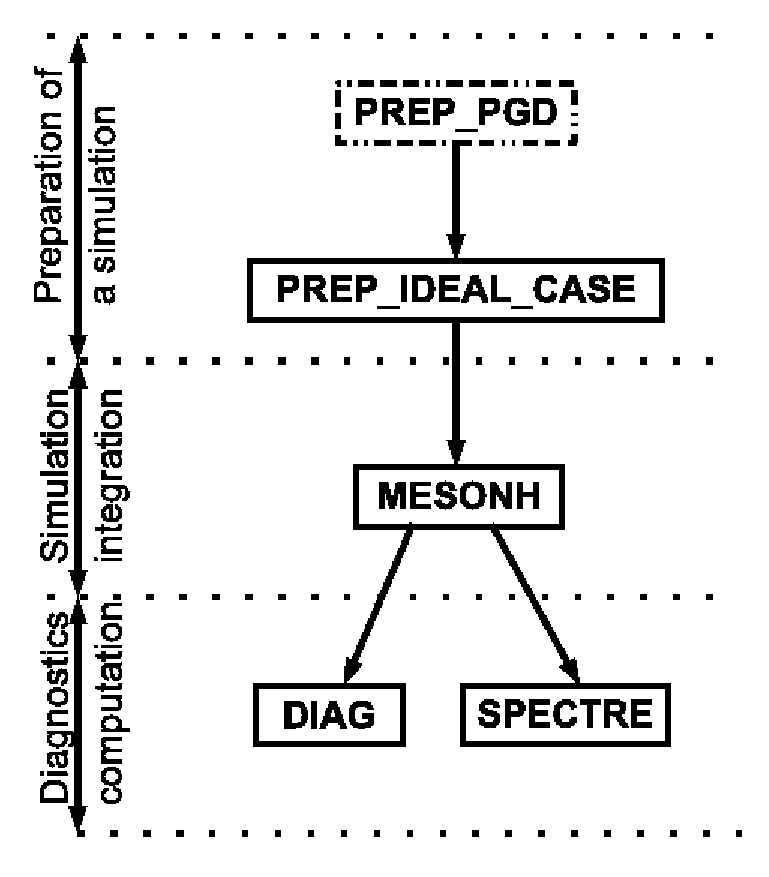
\includegraphics[width=6cm]{intro/magie3}
\\
\textit{Figure 1.1 : General algorithm for an idealized numerical experiment }
\end{center}
\begin{minipage}{8cm}
\vspace{5cm}
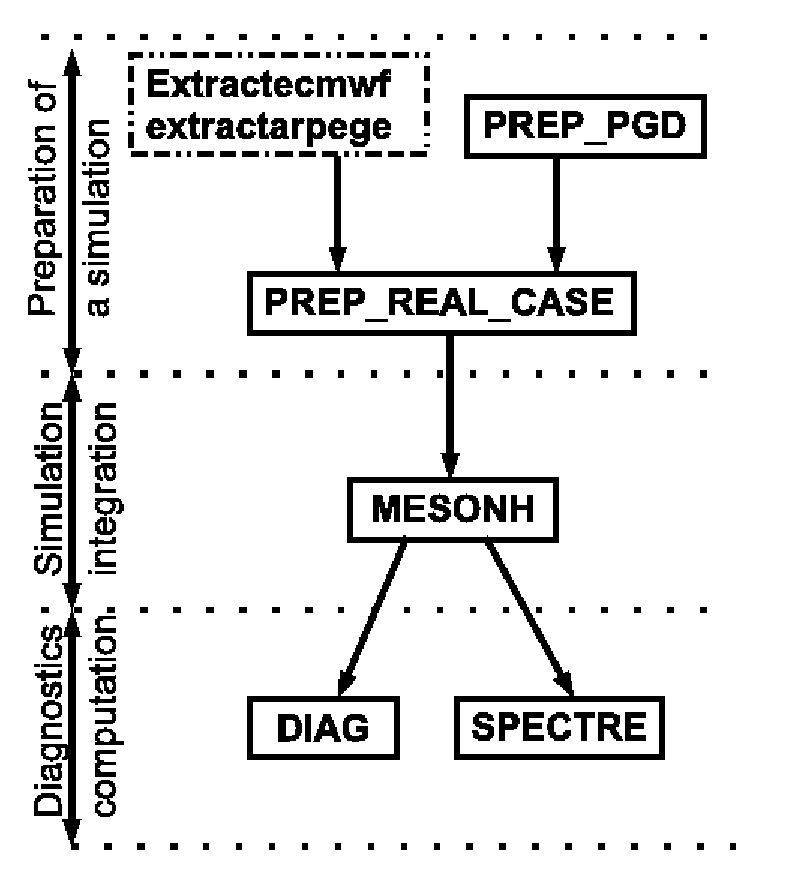
\includegraphics[width=7cm]{intro/magie2}
\begin{center}
\textit{mono-model}
\end{center}
\end{minipage}
\begin{minipage}{9cm}
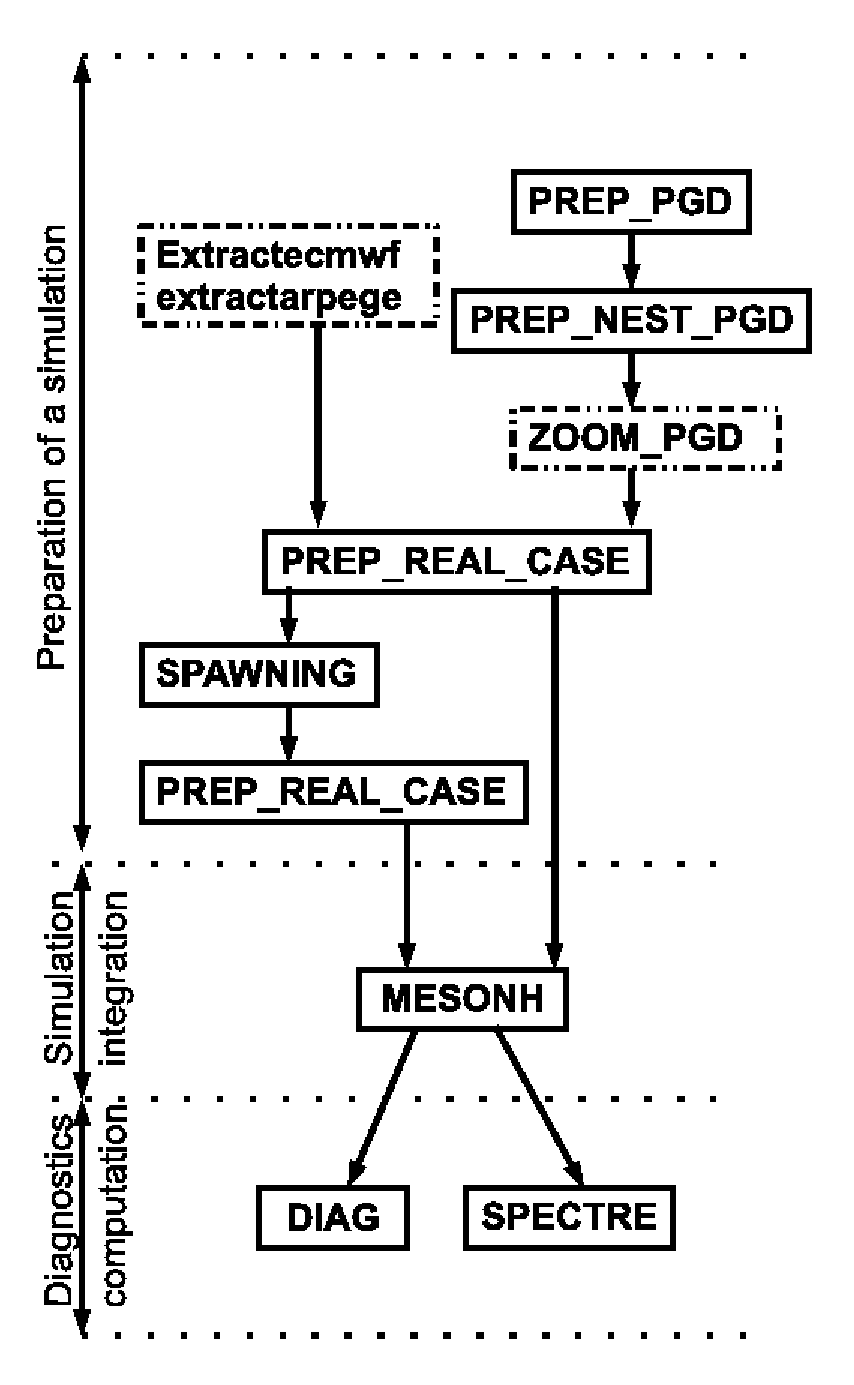
\includegraphics[width=7.5cm]{intro/magie}
\begin{center}
\textit{with grid-nesting}
\end{center}
\end{minipage}
\begin{center}
\textit{Figure 1.2 : General algorithm for a real numerical experiment}
\end{center}




\newpage

First, in chapter 2, installation of Meso-NH is presented and compilation of personal sources is explained.
Then in chapter 3, the Meso-NH files are described in details.
In chapters 4 to 11, every elementary step of Meso-NH is detailed.
In appendix A, all the variables present in a Meso-NH file are listed. In appendix B, sequences for grid-nesting simulation are described. In appendix C, the LES diagnostics is  presented in details. Finally, in appendix D, the Meso-NH grid is shown.



\chapter{Installation of MESONH}

Please follow the instructions given in the file  A-INSTALL.\\
To download this file you have to go in the part "Download" in the mesonh website : \\
\url{http://mesonh.aero.obs-mip.fr/}
	




\chapter{The Meso-NH files}
  
\section{The F90 namelists}

All the information required  to  perform a given step of a numerical
experiment are provided by
different files including a NAMELIST set. 
Thus, the Meso-NH user can change the value of the parameters without
any compilation (and therefore save computer time). These files provide the way 
for the Meso-NH user to interact with the numerical code and finally, they
 contain the identification
cards of the different steps of the numerical experiment. 


These NAMELISTs are Fortran 90
NAMELISTs, which obey to strict writing rules (Metcalf and Reid 1993): no
comment is allowed inside the namelists, no empty namelist can be written (it
gives a Fortran execution error). 

The information are written in the following form:

\begin{verbatim}
 &NAM_LUNITn  CINIFILE = "     FMFILE.1               " /
 &NAM_CONFn  LUSERV = T, LUSERC = F, LUSERR = F, LUSERI = F, LUSERS = F,
 LUSERG = F, LUSERH = F, NSV = 0 /
\end{verbatim}


 {\tt \&NAM\_LUNITn}
is the name of the first namelist of this file, the $/$ character indicates the 
end of the list of information. These namelist  parameters are defined by VAR = VALUE and
these prescriptions are separated from each others by a comma and a blank 
character. Note that you can use more than one line to give a namelist, but in
this case it is imperative to let a blank character at the end of each line.
 
The Meso-NH user does not need to prescribe all the parameters of a namelist,
the missing information are taken equal to the default values
written in the Fortran code. For example, the second namelist in the previous 
example can be written as:
\begin{verbatim}
 &NAM_CONFn  LUSERV = T /
\end{verbatim}
because the other variables of {\tt \&NAM\_CONFn} are set to the default values.
\\

In order to clearly separate what can be modified for a given step of a
numerical experiment, we affect a different namelist file name for each step.

\begin{itemize}
\item
To PREpare a Meso-NH file containing PhysioGraphical Data
\subitem  ${ \large \Longrightarrow } $ file PRE\_PGD1.nam 
\item
To PREpare a Meso-NH file with PhysioGraphical Data in conformity
\subitem  ${ \large \Longrightarrow } $ file PRE\_NEST\_PGD1.nam 
\item
To PREpare a ZOOMed Meso-NH file with PhysioGraphical Data
\subitem  ${ \large \Longrightarrow } $ file PRE\_ZOOM1.nam 
\item
To PREpare an initial Meso-NH file for an IDEAlized case study 
\subitem  ${ \large \Longrightarrow } $ file PRE\_IDEA1.nam 
\item
To PREpare an initial Meso-NH file for an REAL case study 
\subitem  ${ \large \Longrightarrow } $ file PRE\_REAL1.nam 
\item
To SPAWN a Meso-NH file into another one with better horizontal resolution
\subitem  ${ \large \Longrightarrow } $ file SPAWN1.nam 
\item
To EXecute a simulation SEGment for the $n ^{th} $ model
\subitem  ${ \large \Longrightarrow } $ file EXSEGn.nam
\item
To compute DIAGnostics after a simulation
\subitem  ${ \large \Longrightarrow } $ file DIAG1.nam
\end{itemize}


 Because the grid-nesting technique requires the simultanous presence
of multiple models in the computer memory, free-parameters 
must be fixed for every model. This is performed by associating a namelist 
file per model, this explains why the namelist are suffixed by a number 1 or n 
just above.


The different parameters present in these files are all given in this book 
 and more
details on the description of a given parameter are present in the code itself.


\section{The Meso-NH files}

% A Meso-NH FM-file is a set of 2 files, (which can be sticked together via the cpio UNIX
% command):
% \begin{itemize}
% \item
%  a \underline{descriptive part} ( {\tt .des}) containing 
% information about the file generation and its description (in ASCII
% characters)
% \item
% a \underline{binary part} ( {\tt .lfi}) where the fields are stored. The structure of this
%  file is a direct access  type file, written and read by routines developped in
% M\'et\'eo-France (Fischer, 1994) based on {\sc lfi} routines (Clochard, 1989), 
% which can be used on a lot of different computers.
% \end{itemize}

Meso-NH writes files by group of 2:
\begin{itemize}
\item
 a \underline{descriptive part} ({\tt .des}) containing 
information about the file generation and its description (in ASCII
characters)
\item
a \underline{binary part} where the fields are stored. Two different fileformat are available:
  \begin{itemize}
  \item NetCDF (files with a {\tt .nc} suffix). This is the recommanded fileformat and is the default since Meso-NH 5.4.0.
        NetCDF is a self-describing, machine-independent fileformat.
        In Meso-NH, these files are mostly compliant with the CF conventions (version 1.7) and the COMODO extensions (version 1.4).
  \item LFI  (files with a {\tt .lfi} suffix). This is the historic fileformat for Meso-NH. Its structure
        is a direct access type file, written and read by routines developped by
        M\'et\'eo-France (Fischer, 1994) based on {\sc LFI} routines (Clochard, 1989), 
        which can be used on a lot of different computers.
  \end{itemize}
\end{itemize}

These binary files are used to store all the data necessary to run any step 
of a numerical experiment. Three different filetypes are taken into account in the 
Meso-NH project:
\begin{itemize}
\item
the \underline{synchronous backup file} contains all the values of all the fields allowing a
restart of the model and of some diagnostic fields desired by the Meso-NH user.
All these informations are obtained at the same instant during the simulation,
hence their synchronous name.
\item
the \underline{diachronic file} contains time series of information requested by the Meso-NH 
user. They are obtained during more than one time step of the model.
If in LFI fileformat, it is the type in which your file must be if you want to plot it with
the graphics software \tt diaprog \rm (you can convert a synchronous file
into a diachronic one with \tt conv2dia\rm ).
\item
the \underline{physiographic file} contains external information like 
orography, vegetation classes, chemical emissions, data sets, etc.
\end{itemize}

A fourth filetype is possible: output files. They contain only user-selected fields.
They are useful, for example, if you need to output frequently some data without spending too much diskspace
and too much time writing them.


\subsection{The synchronous backup file} \label{ss:synchro}

This type of file contains only information corresponding to the same instant
of the simulation, it remains open during a whole time step of the simulation,
and the writing orders can be given from any routine of the model.

\subsubsection{The descriptive part}
This part is the list of all the namelists of the EXSEG\$n.nam file.
Thus, a complete description of this part is given
with the EXSEG\$n.nam description in chapter \ref{ch:model}.

If the file has been generated during a segment of the model integration, the 
{\tt .des} part contains the different
namelists fixing the free-parameters for the dynamics and the physics 
of the Meso-NH model. This allows the user to know a large
part of the history of this file. For the namelists or variables ommited 
in the EXSEG\$n.nam file, the values are set to the default ones
 (see the tables in ch.\ref{ch:model}).

If the file is the result of the initialization programs 
({\tt PREP\_IDEAL\_CASE}, {\tt PREP\_REAL\_CASE} or {\tt SPAWNING}),
 the values of the namelists variables are the ones of the descriptive part
of the input file of the program if it does exist. Otherwise, the values are
set to the default ones, except for these that can be initialized during the
initialization program (e.g. {\tt CINIFILE} or {\tt LUSERV}).

Note that a physiographic file does not have a descriptive part.

\subsubsection{The binary part}

This type of file can be in netCDF or LFI fileformat.

% All the writings and readings of this type of files are done through LFI 
% routines. A general subroutine to read and write a Meso-NH file is given in the
% Meso-NH library, it provides a file including the fields of the previous record
% list. This Fortran library provides a way to tackle direct access binary files
% and thus a very quick access to the data stored in this file in any order.

It should be noted that additional fields can be added to these basic
information, which have been obtained at the same instant. 
 In order to be easily drawn by the Meso-NH graphic package, the
comment field must be filled, according to the following rules:
\begin{itemize}
\item 
the length of the character string is equal to 100
\item 
the type of the supplementary field must be specified:

\begin{tabular} {|| c |c|| }
\hline
\hline
type & comment field \\
\hline
3D scalar & X\_Y\_Z\_varname  (UNIT) \\
\hline
2D scalar & X\_Y\_varname  (UNIT) \\
\hline
3D vector & VX\_xvarname\_VY\_yvarname\_VZ\_zvarname  (UNIT) \\
\hline
2D scalar & VX\_xvarname\_VY\_yvarname\_VZ\_zvarname  (UNIT) \\
          & or  VX\_xvarname\_VY\_yvarname       (UNIT) \\
\hline
1D scalar & Z\_zvarname  (UNIT) \\
\hline
\hline
\end{tabular}
\end{itemize}

\subsection{The diachronic file}
A diachronic file is a file obtained during a segment of simulation or resulting of the
conversion of a synchronous file with {\tt conv2dia} for graphical purposes (available only for LFI fileformat).

The file directly obtained during the simulation has a name ended by {\tt .000},
and contains records such as averaged variables, tendencies, fluxes stored
at different times of the simulation on the whole or some parts of the domain.
Such records are obtained by requesting temporal series (\ref{ss:series}),
budgets (\ref{ss:budget}), aircraft or balloon (\ref{ss:balloon}), profiler
or station (\ref{ss:station}), or LES diagnostics (\ref{s:LESdiag}).

\subsection{The physiographic file}
It is a bidimensional MesoNH file with contains surface data such as orography,
vegetation classes, chemical emissions, etc.

See the documentation: ''Surfex user's guide'' for more
details.

\subsection{The output file}
An output file is obtained at the user request. They are written at once for a given timestep.
They contain only user-selected fields.
They are useful, for example, if you need to output frequently some data without spending too much diskspace
and too much time writing them.

In contrast to the synchronous backup files, output files does not contain enough information to restart a calculation. Furthermore, they are not associated with a descriptive file.


\section{References}
\decrefname
J. Clochard, 1989: Logiciel de Fichiers Index\'es. Direction de la
 Météorologie Nationale. Note de travail ARPEGE n$^\circ$12.

\decrefname
J. Clochard, 1991: Logiciel de Fichiers Index\'es. Direction de la
 Météorologie Nationale.  Technical report.

\decrefname
D. Gazen, 1999: Parallel IO routines. Man page on Meso-NH web site.

\decrefname
C. Fischer, 1994: File structure and content in the Meso-NH model. Meso-NH note.

\chapter{Creation of MESO-NH physiographic data file} \label{c:PGD}


\section{\bf PREP\_PGD}
The physiographic fields are averaged or interpolated on the MESO-NH
physiographic grid by the program {\bf PREP\_PGD}. 
They are stored in a FM file, called PGD file, but with fewer elements than a MESO-NH file.
With the physiographic 2D fields, the geographic and grid data
are written in this file.
Note that a MESO-NH simulation runs on the grid defined here in 
{\bf PREP\_PGD}. \\

\subsection{Namelist NAM\_CONFIO}
See section \ref{s:namconfio} page \pageref{s:namconfio} for details.

\subsection{Namelist NAM\_CONF\_PGD}
\index{NAM\_CONF\_PGD!namelist description}
\begin{center}
\begin{tabular} {|l|l|l|}
\hline
Fortran name & Fortran type & default value\\
\hline
\hline
NHALO\_MNH  & INTEGER & 1 \\
JPHEXT      & INTEGER & 1 \\
\hline
\end{tabular}
\end{center}

\begin{itemize}
\item
NHALO\_MNH: Size of the halo for parallel distribution.
This variable is related to computer performance but has no
impact on simulation results.\\
\index{NHALO\_MNH!\innam{NAM\_CONF\_PGD}}

\item
JPHEXT:  Horizontal External points number\\
JPHEXT must be equal to 3 for cyclic cases with WENO5.
\index{JPHEXT!\innam{NAM\_CONF\_PGD}}
\end{itemize}



\subsection{Namelist NAM\_PGDFILE}
\index{NAM\_PGDFILE!namelist description}

\begin{center}
\begin{tabular} {|l|l|l|}
\hline
Fortran name & Fortran type & default value\\
\hline
\hline
CPGDFILE      & character (LEN=28) & ' '           \\
NHALO         & INTEGER      & 15 \\
\hline
\end{tabular}
\end{center}

\begin{itemize}
\item CPGDFILE : name of the output Physiographic Data File
\index{CPGDFILE!\innam{NAM\_PGDFILE}}
\item NHALO :  Size of the halo for parallel distribution
\index{NHALO!\innam{NAM\_PGDFILE}}

\end{itemize}
\subsection{Namelist NAM\_ZSFILTER}
\index{NAM\_ZSFILTER!namelist description}

\begin{center}
\begin{tabular} {|l|l|l|}
\hline
Fortran name & Fortran type & default value\\
\hline
\hline
NZSFILTER       & INTEGER      & 1 \\
LHSLOP       & LOGICAL      & .FALSE. \\
XHSLOP       & REAL      & 1.2 \\
NLOCZSFILTER & INTEGER & 3 \\
\hline
\end{tabular}
\end{center}

\begin{itemize}
\item NZSFILTER : number of iterations of the spatial filter applied to smooth the orography over the whole domain (integer, 1 iteration removes the $2\Delta x$ signal, 50\% of the $4\Delta x$
signal, 25\% of the $6\Delta x$ signal, etc\footnote{The amplitude of the
filtered signal for each wavelength $\lambda\Delta x$ 
is $\frac{1}{2}\left( cos(2\pi/\lambda) +1\right)$.}...).
\index{NZSFILTER!\innam{NAM\_ZSFILTER}}
\item LHSLOP : flag to use a spatial filter applied to smooth the orography locally over the slopes (along the horizontal directions) higher than XHSLOP.
\index{LHSLOP!\innam{NAM\_ZSFILTER}}
\item XHSLOP : slope threshold ($\Delta z / $\Delta x$ and $\Delta z / $\Delta y$) where the local spatial filter is applied.
\index{XHSLOP!\innam{NAM\_ZSFILTER}}
\item NLOCZSFILTER : number of iterations of the local spatial filter applied to smooth the large slopes.
\index{NLOCZSFILTER!\innam{NAM\_ZSFILTER}}

\end{itemize}
%\newpage
\subsection{Namelists for the externalized surface}

As indicated above, further definition of surface parameters are not done by MESONH itself, but by the externalized surface included in it. For more informations see SURFEX documentation.\\

\begin{itemize}
\item NAM\_PGD\_SCHEMES\index{NAM\_PGD\_SCHEMES!surfex namelist}
\item NAM\_PGD\_GRID\index{NAM\_PGD\_GRID!surfex namelist}
\item NAM\_CONF\_PROJ\index{NAM\_CONF\_PROJ!surfex namelist}
\item NAM\_CONF\_PROJ\_GRID\index{NAM\_CONF\_PROJ\_GRID!surfex namelist}
\item NAM\_INIFILE\_CONF\_PROJ\index{NAM\_INIFILE\_CONF\_PROJ!surfex namelist}
\item NAM\_WRITE\_COVER\_TEX\index{NAM\_WRITE\_COVER\_TEX!surfex namelist}
\item NAM\_READ\_DATA\_COVER\index{NAM\_READ\_DATA\_COVER!surfex namelist}
\item NAM\_PGD\_ARRANGED\_COVER\index{NAM\_PGD\_ARRANGED\_COVER!surfex namelist}
\item NAM\_COVER\index{NAM\_COVER!surfex namelist}
\item NAM\_ECOCLIMAP2\index{NAM\_ECOCLIMAP2!surfex namelist}
\item NAM\_ZS\index{NAM\_ZS!surfex namelist}
\item NAM\_SEABATHY\index{NAM\_SEABATHY!surfex namelist}
\item NAM\_ISBA\index{NAM\_ISBA!surfex namelist}
\item NAM\_DATA\_FLAKE\index{NAM\_DATA\_FLAKE!surfex namelist}
\item NAM\_DUMMY\_PGD\index{NAM\_DUMMY\_PGD!surfex namelist}
\item NAM\_CH\_EMIS\_PGD\index{NAM\_CH\_EMIS\_PGD!surfex namelist}
\end{itemize}

\subsection{Examples of PRE\_PGD1.nam file \label{example}}

A {\bf PREP\_PGD} run where you use the data files provided by the MESO-NH team and some files of your own for the dummy fields:
\begin{verbatim}
&NAM_PGDFILE        CPGDFILE = 'PGDFILE_1' /
&NAM_PGD_GRID       CGRID = 'CONF PROJ ' /
&NAM_CONF_PROJ      XLAT0 = 45., XLON0=0., XRPK=0.7, XBETA=0. /
&NAM_CONF_PROJ_GRID NIMAX=100, NJMAX=100, XLATCEN=42.5, XLONCEN=2.5, XDX=10000. , XDY=10000. /
&NAM_INIFILE_CONF_PROJ /
&NAM_PGD_SCHEMES CNATURE='ISBA  ', CSEA='SEAFLX', CTOWN='TEB   ', CWATER='WATFLX' /
&NAM_COVER YCOVER='ecoclimap_v2', YCOVERFILETYPE='DIRECT' /
&NAM_ZS    YZS='gtopo30', YZSFILETYPE='DIRECT' /
&NAM_ISBA  YCLAY='clay_fao', YCLAYFILETYPE='DIRECT',  XUNIF_RUNOFFB=0.5 ,
           YSAND='sand_fao', YSANDFILETYPE='DIRECT' /
&NAM_DUMMY_PGD  NDUMMY_NBR         = 6
                CDUMMY_NAME(1)     = 'SST_2001062100'          
                CDUMMY_AREA(1)     = 'SEA'
                CDUMMY_ATYPE(1)    = 'ARI'
                CDUMMY_FILE(1)     = 'SSTn2001062100.dat'          
                CDUMMY_FILETYPE(1) = 'ASCLLV'
                CDUMMY_NAME(2)     = 'SST_2001062200'          
                CDUMMY_AREA(2)     = 'SEA'
                CDUMMY_ATYPE(2)    = 'ARI'
                CDUMMY_FILE(2)     = 'SSTn2001062200.dat'          
                CDUMMY_FILETYPE(2) = 'ASCLLV'
                CDUMMY_NAME(3)     = 'SST_2001062300'          
                CDUMMY_AREA(3)     = 'SEA'
                CDUMMY_ATYPE(3)    = 'ARI'
                CDUMMY_FILE(3)     = 'SSTn2001062300.dat'          
                CDUMMY_FILETYPE(3) = 'ASCLLV'
                CDUMMY_NAME(4)     = 'SST_2001062400'          
                CDUMMY_AREA(4)     = 'SEA'
                CDUMMY_ATYPE(4)    = 'ARI'
                CDUMMY_FILE(4)     = 'SSTn2001062400.dat'          
                CDUMMY_FILETYPE(4) = 'ASCLLV'
                CDUMMY_NAME(5)     = 'SST_2001062500'          
                CDUMMY_AREA(5)     = 'SEA'
                CDUMMY_ATYPE(5)    = 'ARI'
                CDUMMY_FILE(5)     = 'SSTn2001062500.dat'          
                CDUMMY_FILETYPE(5) = 'ASCLLV'
                CDUMMY_NAME(6)     = 'SST_2001062600'          
                CDUMMY_AREA(6)     = 'SEA'
                CDUMMY_ATYPE(6)    = 'ARI'
                CDUMMY_FILE(6)     = 'SSTn2001062600.dat', CDUMMY_FILETYPE(6) = 'ASCLLV'/
\end{verbatim}
\newpage
Another {\bf PREP\_PGD} run for the father PGD file, with all the namelist variables : 
\begin{verbatim}
&NAM_PGDFILE CPGDFILE='PGD_AMMA1_10km_m46_b1' /
&NAM_PGD_SCHEMES  CNATURE='ISBA' , CSEA='SEAFLX', CWATER='WATFLX', CTOWN='TEB'/
&NAM_PGD_GRID CGRID='CONF PROJ'/
&NAM_CONF_PROJ   XLAT0=13. ,XLON0=-1.5, XRPK=0.2249510543, XBETA=0 /
&NAM_CONF_PROJ_GRID  XLATCEN=13. , XLONCEN=-1.5 , NIMAX=324 ,NJMAX=240 ,
                     XDX=10000 , XDY=10000/
&NAM_COVER     YCOVER='ecoclimats_v2', YCOVERFILETYPE='DIRECT',LRM_TOWN=.FALSE. /
&NAM_ZS        YZS='gtopo30',    YZSFILETYPE='DIRECT' ,
               COROGTYPE='AVG', XENV=0./
&NAM_ISBA      NPATCH=12, CISBA='3-L',  CPHOTO='AGS', NGROUND_LAYER=3, 
               YCLAY='clay_fao', YCLAYFILETYPE='DIRECT' ,
               YSAND='sand_fao', YSANDFILETYPE='DIRECT',
               XUNIF_RUNOFFB=0.5 /
&NAM_CH_EMIS_PGD NEMIS_PGD_NBR=0 /               
&NAM_DUMMY_PGD  NDUMMY_PGD_NBR=0 /
\end{verbatim}

And for the son PGD file : 
\begin{verbatim}
&NAM_PGDFILE CPGDFILE='PGD_AMMA1_5km_m46_b1' /
&NAM_PGD_SCHEMES  CNATURE='ISBA' , CSEA='SEAFLX', CWATER='WATFLX', CTOWN='TEB'/
&NAM_PGD_GRID YINIFILE='PGD_AMMA1_10km_m46_b1',YINIFILETYPE='MESONH' /
&NAM_INIFILE_CONF_PROJ IXOR=101 ,IYOR=21 ,IXSIZE=180 ,IYSIZE=150 ,
                       IDXRATIO=2, IDYRATIO=2/
&NAM_COVER     YCOVER='ecoclimats_v2', YCOVERFILETYPE='DIRECT',LRM_TOWN=.FALSE. /
&NAM_ZS        YZS='gtopo30', YZSFILETYPE='DIRECT' ,
               COROGTYPE='AVG', XENV=0./
&NAM_ISBA      NPATCH=12, CISBA='3-L',  CPHOTO='AGS', NGROUND_LAYER=3, 
               YCLAY='clay_fao', YCLAYFILETYPE='DIRECT' ,
               YSAND='sand_fao', YSANDFILETYPE='DIRECT',
               XUNIF_RUNOFFB=0.5 /
&NAM_CH_EMIS_PGD NEMIS_PGD_NBR=0 /               
&NAM_DUMMY_PGD  NDUMMY_PGD_NBR=0 /
\end{verbatim}

%%%%%%%%%%%%%%%%%%%%%%%%%%%%%%%%%%%%%%%%%%%%%%%%%%%%%%%%%%%%%%%
\newpage
\section{Modification of PGD files for grid-nesting: {\bf
PREP\_NEST\_PGD}}

In order to run models with the gridnesting technique, a condition on
the orography must be satisfied. In the following, if file \#2 is completely
included in (and therefore in interaction during the run with) file \#1,
file \#2 will be called the SON file, and file \#1 the DAD file.
In the following, the DAD file number must be smaller than any of its SON number.

The condition on the orography is:
"the mean of orography for a SON file in the domain corresponding to the
grid mesh of its DAD file, must be equal to the orography of the DAD file
in this mesh".

Such a condition is not automatically satisfied when using enhanced
orographies.
The program {\bf PREP\_NEST\_PGD} performs post-treatments on the orographies
of up to 8 PGD files that will be used to create initialization files 
for a gridnested run. It modifies the orography of a DAD from the mean
of the orography of its (several) SON(s).



The namelist file PRE\_NEST\_PGD1.nam contains:
\begin{enumerate}
\item
\underline{Namelists NAM\_PGD{\it \bf{N}}} (where {\it \bf{N}} goes from 1 to 8):
\index{YPGD1!\innam{NAM\_PGD1}}
\index{YPGD2!\innam{NAM\_PGD2}}
\index{YPGD3!\innam{NAM\_PGD3}}
\index{YPGD4!\innam{NAM\_PGD4}}
\index{YPGD5!\innam{NAM\_PGD5}}
\index{YPGD6!\innam{NAM\_PGD6}}
\index{YPGD7!\innam{NAM\_PGD7}}
\index{YPGD8!\innam{NAM\_PGD8}}
\index{IDAD!\innam{NAM\_PGD1}}
\index{IDAD!\innam{NAM\_PGD2}}
\index{IDAD!\innam{NAM\_PGD3}}
\index{IDAD!\innam{NAM\_PGD4}}
\index{IDAD!\innam{NAM\_PGD5}}
\index{IDAD!\innam{NAM\_PGD6}}
\index{IDAD!\innam{NAM\_PGD7}}
\index{IDAD!\innam{NAM\_PGD8}}
\begin{itemize}
\item YPGD{\it \bf{N}}: name of the PGD file \#{\it \bf{N}}
\item IDAD: number of the DAD file of file \#{\it \bf{N}}.
The DAD file number IDAD must be \underline{smaller} than \#{\it \bf{N}}.
\end{itemize}
\bigskip
\item
\underline{Namelist NAM\_NEST\_PGD}:
\begin{itemize}
\item
YNEST: string of 2 characters to be added to the PGD file names to define
the corresponding output PGD file names. The input file {\it YPGD{\bf N}}
will be modified into file {\it YPGD{\bf N}}.nest{\it YNEST}
\index{YNEST!\innam{NAM\_NEST\_PGD}}
\end{itemize}

\bigskip
\item
\underline{Namelist NAM\_CONFIO}:
See section \ref{s:namconfio} page \pageref{s:namconfio} for details.

\bigskip
\item
\underline{Namelist NAM\_CONF\_NEST} :
\index{NAM\_CONF\_NEST!namelist description}
\begin{center}
\begin{tabular} {|l|l|l|}
\hline
Fortran name & Fortran type & default value\\
\hline
\hline
NHALO\_MNH  & INTEGER & 1 \\
JPHEXT      & INTEGER & 1 \\
\hline
\end{tabular}
\end{center}

\begin{itemize}
\item
NHALO\_MNH: Size of the halo for parallel distribution.
This variable is related to computer performance but has no
impact on simulation results.\\
NHALO must be equal to 3 for WENO5 cases in parallel runs
\index{NHALO!\innam{NAM\_CONF\_NEST}}

\item
JPHEXT:  Horizontal External points number\\
JPHEXT must be equal to 3 for cyclic cases with WENO5.
\index{JPHEXT!\innam{NAM\_CONF\_NEST}}
\end{itemize}

\end{enumerate}



\underline{Example of namelist PRE\_NEST\_PGD1.nam:}
\begin{verbatim}
&NAM_PGD1 YPGD1 = 'PGDFILE_1' /
&NAM_PGD2 YPGD2 = 'PGDFILE_2', IDAD = 1 /
&NAM_PGD3 YPGD3 = 'PGDFILE_3', IDAD = 1 /
&NAM_PGD4 YPGD4 = 'PGDFILE_4', IDAD = 3 /
&NAM_PGD5 YPGD5 = 'PGDFILE_5', IDAD = 2 /
&NAM_PGD6  /
&NAM_PGD7  /
&NAM_PGD8  /
&NAM_NEST_PGD YNEST = 'e1' /
\end{verbatim}

%%%%%%%%%%%%%%%%%%%%%%%%%%%%%%%%%%%%%%%%%%%%%%%%%%%%%%%%%%%%%%%

\section{Zoom of a PGD file: {\bf ZOOM\_PGD}}
The previous condition on the orography needed
when using the gridnesting technique implies that all the PGD files have to be
created (with {PREP\_PGD} and {PREP\_NEST\_PGD} programs)
{\bf before} beginning the run.
However, the user is not always sure where (and when) to initialize
the inner models.
To avoid to set exactly the domain of inner models at the PREP\_PGD step, 
one solution is to make PGD file on larger domain
and then, zoom it\footnote{This was done during the PREP\_IDEAL\_CASE or 
PREP\_REAL\_CASE step before the masdev4\_6 version.}
 on the part of the domain of interest when known
with the following program {\bf ZOOM\_PGD}. Then the output PGD file is used
as PGD file for the interpolations of atmospheric fields
with {SPAWNING} and {PREP\_REAL\_CASE} programs. 



The namelist file PRE\_ZOOM1.nam contains 2 namelists:
\begin{enumerate}
\item
\underline{Namelist NAM\_PGDFILE}: (contains file names)
\index{NAM\_PGDFILE!namelist description}

\begin{center}
\begin{tabular} {|l|l|l|}
\hline
Fortran name & Fortran type & default value\\
\hline
\hline
CPGDFILE      & character (LEN=28) & 'PGDFILE'      \\
YZOOMFILE     & character (LEN=28) & none           \\
YZOOMNBR      & character (LEN=2)  & '00'           \\
\hline
\end{tabular}
\end{center}

\begin{itemize}
\item CPGDFILE : name of the input Physiographic Data File
\index{CPGDFILE!\innam{NAM\_PGDFILE}}
\item YZOOMFILE : optional name of the zoomned FM-file (output file).
\index{YZOOMFILE!\innam{NAM\_PGDFILE}} 
If the user does not specify this name,
or if YZOOMFILE = CPGDFILE, the code builds the zoomned FM-file name as:
\subitem YZOOMFILE = CPGDFILE.zYZOOMNBR
\item YZOOMNBR :
\index{YZOOMNBR!\innam{NAM\_PGDFILE}} :
NumBeR which will be added to CPGDFILE to generate the  
name of the Zoomned FM-file (string of 2 characters).
\end{itemize}
\item
\underline{Namelist NAM\_CONFIO}
See section \ref{s:namconfio} page \pageref{s:namconfio} for details.
\item
\underline{Namelist NAM\_MESONH\_DOM}: (contains domain definition variables)
\index{NAM\_MESONH\_DOM!namelist description}

\begin{center}
\begin{tabular} {|l|l|l|l|}
\hline
Fortran name & Fortran type & default value & remarks \\
\hline
\hline
NIMAX & integer & input PGD domain & \\
NJMAX & integer & input PGD domain & \\
NXOR  & integer & NUNDEF & if NUNDEF, domain is \\ 
      &         &        & in the middle of PGD \\ 
NYOR  & integer & NUNDEF & if NUNDEF, domain is \\ 
      &         &        & in the middle of PGD \\ 
\hline
\end{tabular}
\end{center}

\begin{itemize}
\item NIMAX : number of grid points in I direction, according to input file 
grid, recovered by the new domain. NIMAX must be equal to $2^m \times 3^n \times 5^p$ with $(m,n,p) \in [0,+\infty[$
\index{NIMAX!\innam{NAM\_MESONH\_DOM}}
\item NJMAX : number of grid points in J direction, according to input file 
grid, recovered by the new domain. NJMAX must be equal to $2^m \times 3^n \times 5^p$ with $(m,n,p) \in [0,+\infty[$
\index{NJMAX!\innam{NAM\_MESONH\_DOM}}
\item NXOR : first point I index, left to and out of the new physical domain.
\index{NXOR!\innam{NAM\_MESONH\_DOM}}
\item NYOR : first point J index, under and out of the new physical domain.
\index{NYOR!\innam{NAM\_MESONH\_DOM}}
\end{itemize}

\end{enumerate}

\underline{Example of namelist PRE\_ZOOM1.nam:}
\begin{verbatim}
&NAM_PGDFILE CPGDFILE = 'PGDFILE_1.neste1' ,
             YZOOMNBR = '58'    /
&NAM_MESONH_DOM NIMAX=60, NJMAX=50,
                NXOR=5, NYOR=8      /
\end{verbatim}



\chapter{Preparation of an ideal simulation : PREP\_IDEAL\_CASE}\label{c:PREPIDEAL}

\section{Overview of PREP\_IDEAL\_CASE functionalities}


The "PREP\_IDEAL\_CASE" program  prepares a MESONH file, that contains all the
parameters and fields necessary for the execution of the MESONH model.
Specifically, the grid parameters, the initial fields and the geophysical fields
are included in this file. It is possible using this program to generate
idealized fields defined by few parameters.\\ 

The generated initial conditions are produced analytically, leading to 
 quasi-1D fields or 3D fields or a single profile build with either:
\begin{itemize}
\item
layers of constant Brunt-Vaisala frequency, shear  and 
humidity  
\item a Radiosounding and ideal surface fields
\item a Radiosounding and real physiographic fields 
\item
a Radiosounding and real and ideal surface fields at the same time
\end{itemize}

For these latter cases, the initial fields may be  hydrostatically or
geostrophically  balanced or not.
For these fields to satisfy the anelastic constraint, a final correction is
applied to them.


The interaction between the PREP\_IDEAL\_CASE program and the user is made through 
the PRE\_IDEA1.nam file. The degrees of freedom  are collected in a set of
namelists,  read by this program. 

\newpage
\section {The input: the PRE\_IDEA1.nam file}

It is made  of  two parts :

\begin{itemize}
\item A namelist-part with directives for the preparation
of an idealized case (always present).  The
order of namelists is free and unset namelists can be ommited.
\item A free-formatted part describing
a vertical profile of n layers of constant moist Brunt-Vaisala frequency or
a radiosounding and sometimes the explicit list of the heights of the vertical
levels. This part can be present or absent in the other cases.

\end{itemize}

To initialize a simulation with a radiosounding and real
terrain conditions, it is necessary to perform the PREP\_PGD program 
to create a MESO-NH physiographic data file. This data file contains
 the orography and the physiographic data fields (related to the soil scheme).
It is also possible to perform a complete ideal case with ideal orography and 
non trivial surface conditions.
The user can combine the two possibilities with flags included in the namelist 
NAM\_REAL\_PGD and initialize a simulation with a real orography and
idealized homogeneous surface fields.
If a PREP\_PGD file is specified and if the flags in namelist NAM\_REAL\_PGD
are set to FALSE, homogeneous values can be imposed by the user in namelists 
from the externalized surface facility PGD (namelists NAM\_COVER and NAM\_ISBA),
else the PREP\_PGD fields are taken into account.
\\

In the following, the namelists are listed in alphabetical order.
\newpage
\subsection{Namelist NAM\_AERO\_PRE (init. aerosol scalar variables)} \label{s:namaeropre}
\index{NAM\_AERO\_PRE!namelist description}

If you initialize aerosol during PREP\_IDEAL\_CASE as for ORILAM (chemical aerosols), DUST and SEA SALT.
use the following namelist variables:
\begin{center}
\begin{tabular} {|l|l|l|}
\hline
Fortran name & Fortran type & default value \\
\hline
LORILAM      & logical       & FALSE    \\
LDUST        & logical       & FALSE    \\
LSALT        & logical       & FALSE    \\
LINITPM      & logical       & FALSE    \\
XINIRADIUSI  & real          & 0.05     \\
XINIRADIUSJ  & real          & 0.2      \\
XINISIGI     & real          & 1.8      \\
XINISIGJ     & real          & 2.0      \\
XN0IMIN      & real          & 10.      \\
XN0JMIN      & real          & 1.       \\
CRGUNIT      & character     & "NUMB"   \\
NMODE\_DST   & integer       & 3       \\
XN0MIN       & real          & 1.e3 , 1.e1 , 1.e-2 \\
XINIRADIUS   & real          & 0.044, 0.3215, 1.575 \\
XINISIG      & real          & 2.0, 1.78, 1.85 \\
CRGUNITD     & character     & "NUMB"   \\
NMODE\_SLT   & integer       & 3       \\
XN0MIN\_SLT  & real          & 1.e4 , 1.e2 , 1.e-1 \\
XINIRADIUS\_SLT & real       & 0.14, 1.125,  7.64\\
XINISIG\_SLT    & real       & 1.9, 2., 2. \\
CRGUNITS     & character     & "MASS"   \\
\hline
\end{tabular}
\end{center}

\begin{itemize}
\item LORILAM\index{LORILAM!\innam{NAM\_AERO\_PRE}}:
Flag to activate  chemical aerosol initialization (only if LCH\_INIT\_FIELD=T in NAM\_CH\_MNHCn\_PRE).
\item LDUST\index{LDUST!\innam{NAM\_AERO\_PRE}}: 
Flag to activate  passive dust initialization (3 modes).
\item LSALT\index{LSALT!\innam{NAM\_AERO\_PRE}}: 
Flag to activate  passive sea salt initialization (3 modes).
\item LINITPM\index{LINITPM!\innam{NAM\_AERO\_PRE}}:
Flag to activate  primary aerosol initialization (Black and Organic carbon) from concentration of CO (only if LORILAM=T in NAM\_CH\_MNHCn\_PRE).
\item XINIRADIUSI\index{XINIRADIUSI!\innam{NAM\_AERO\_PRE}}:
Initial mean radius of aitken mode in $\mu m$  (only if LORILAM=T \\
in NAM\_AERO\_PRE).
\item XINIRADIUSJ\index{XINIRADIUSJ!\innam{NAM\_AERO\_PRE}}:
Initial mean radius of accumulation mode in $\mu m$ (only if LORILAM=T in NAM\_AERO\_PRE).
\item XINISIGI\index{XINISIGI!\innam{NAM\_AERO\_PRE}}:
Initial standard deviation of aitken  mode (only if LORILAM=T in NAM\_AERO\_PRE).
\item XINISIGJ\index{XINISIGJ!\innam{NAM\_AERO\_PRE}}:
Initial standard deviation of accumulation  mode (only if LORILAM=T in NAM\_AERO\_PRE).
\item XN0IMIN\index{XN0IMIN!\innam{NAM\_AERO\_PRE}}:
Minimum number concentration of aitken mode (only if LORILAM=T in NAM\_AERO\_PRE).
\item XN0JMIN\index{XN0JMIN!\innam{NAM\_AERO\_PRE}}:
Minimum number concentration of accumulation mode (only if LORILAM=T in NAM\_AERO\_PRE).
\item CRGUNIT\index{CRGUNIT!\innam{NAM\_AERO\_PRE}}:
Definition of XINIRADIUSI or XINIRADIUSJ: mean radius is in mass or in number; possible values are MASS or NUMB (only if LORILAM=T in NAM\_AERO\_PRE).
\item NMODE\_DST\index{NMODE\_DST!\innam{NAM\_AERO\_PRE}}:
Number of DUST mode (between 1 and 3 and only if LDUST=T in NAM\_AERO\_PRE).
\item XN0MIN\index{XN0MIN!\innam{NAM\_AERO\_PRE}}:
Minimum number concentration of the NMODE\_DST in particles by m3 (only if LDUST=T in NAM\_AERO\_PRE).
\item XINIRADIUS\index{XINIRADIUS!\innam{NAM\_AERO\_PRE}}:
Initial mean radius of the NMODE\_DST modes in $\mu m$ (only if LDUST=T in NAM\_AERO\_PRE). 
\item XINISIG\index{XINISIG!\innam{NAM\_AERO\_PRE}}:
Initial standard deviation of the NMODE\_DST modes (only if LDUST=T in NAM\_AERO\_PRE). 
\item CRGUNITD\index{CRGUNITD!\innam{NAM\_AERO\_PRE}}:
Definition of XINIRADIUS : mean radius is in mass or in number; possible values are MASS or NUMB (only if LDUST=T in NAM\_AERO\_PRE).
\item NMODE\_SLT\index{NMODE\_SLT!\innam{NAM\_AERO\_PRE}}:
Number of SALT mode in $\mu m$ (between 1 and 3 and only if LSALT=T in NAM\_AERO\_PRE).
\item XN0MIN\_SLT\index{XN0MIN\_SLT!\innam{NAM\_AERO\_PRE}}:
Minimum number concentration of the NMODE\_SLT in particles by m3 (only if LSALT=T in NAM\_AERO\_PRE).
\item XINIRADIUS\_SLT\index{XINIRADIUS\_SLT!\innam{NAM\_AERO\_PRE}}:
Initial mean radius of the NMODE\_SLT modes (only if LSALT=T in NAM\_AERO\_PRE).
\item XINISIG\_SLT\index{XINISIG\_SLT!\innam{NAM\_AERO\_PRE}}:
Initial standard deviation of the NMODE\_SLT modes (only if LSALT=T in NAM\_AERO\_PRE).
\item CRGUNITS\index{CRGUNITS!\innam{NAM\_AERO\_PRE}}:
Definition of XINIRADIUS\_SLT : mean radius is in mass or in number; possible values are MASS or NUMB (only if LSALT=T in NAM\_AERO\_PRE).
\end{itemize}


\subsection{Namelist NAM\_BLANKn (available user variables)} \label{s:namblank}
\index{NAM\_BLANKn !namelist description}
\begin{center}
\begin{tabular} {|l|l|l|}
\hline
Fortran name & Fortran type & default value \\
\hline
XDUMMY1 .. XDUMMY8 & real                 & 0.       \\
NDUMMY1 .. NDUMMY8 & integer              & 0        \\
LDUMMY1 .. LDUMMY8 & logical              & TRUE     \\
CDUMMY1 .. CDUMMY8 & 80 characters        & ''       \\
XDUMMY             & array(real)          & 20* 0.   \\
NDUMMY             & array(integer)       & 20* 0    \\
LDUMMY             & array(logical)       & 20* TRUE \\
CDUMMY             & array(80 characters) & 20* ''   \\
\hline
\end{tabular}
\end{center}

Eight dummy, real, integer, logical and character*80 variables and
arrays of dummy, real, integer, logical and character*80 for test
and debugging  purposes are defined and passed through the namelist
read operations. None of the MesoNH routines uses any of these
variables. When a developper choses to introduce temporarily a
parameter to some subroutine, he has to introduce a USE MODD\_BLANKn
statement into that subroutine. Then he can use any of the variables
defined here and change them easily via the namelist input.



\subsection{Namelist NAM\_CH\_MNHCn\_PRE (init. chemistry scalar variables)}

If you initialize MNH-C using PREP\_IDEAL\_CASE,
use the following namelist variables:
\begin{center}
\begin{tabular} {|l|l|l|}
\hline
Fortran name & Fortran type & default value \\
\hline
LCH\_INIT\_FIELD  & logical       & FALSE      \\
CCHEM\_INPUT\_FILE & 80 characters & MNHC.input \\
\hline
\end{tabular}
\end{center}

\begin{itemize}

\item LCH\_INIT\_FIELD\index{LCH\_INIT\_FIELD!\innam{NAM\_CH\_MNHCn\_PRE}}: 
Flag to activate initialization subroutine CH\_INIT\_FIELD.

\item CCHEM\_INPUT\_FILE\index{CCHEM\_INPUT\_FILE!\innam{NAM\_CH\_MNHCn\_PRE}}:
 name of the general purpose input file for initialization.
 

\end{itemize}


\subsection{Namelist NAM\_CONFIO}
See section \ref{s:namconfio} page \pageref{s:namconfio} for details.


\subsection{Namelist NAM\_CONF\_PRE  (configuration variables)}
\index{NAM\_CONF\_PRE!namelist description}

\begin{center}
\begin{tabular} {|l|l|l|}
\hline
Fortran name & Fortran type & default value \\
\hline
LCARTESIAN & logical     & TRUE  \\
LPACK      & logical     & TRUE  \\
CEQNSYS    & 3 characters& 'DUR'   \\
NVERB      & integer     & 5     \\
CIDEAL     & 4 characters& 'CSTN'  \\
CZS        & 4 characters& FLAT  \\
LBOUSS     & logical     & FALSE \\
LPERTURB   & logical     & FALSE \\
LFORCING   & logical     & FALSE \\
LSHIFT     & logical     & FALSE \\
L2D\_ADV\_FRC  & logical     & FALSE \\
L2D\_REL\_FRC  & logical     & FALSE \\
NHALO      & integer        & 1      \\
JPHEXT     & integer        & 1      \\
LOCEAN     & logical        & FALSE \\
\hline
\end{tabular}
\end{center}

\begin{itemize}

\item  LCARTESIAN \index{LCARTESIAN!\innam{NAM\_CONF\_PRE}}
: Flag for cartesian geometry 
\begin{itemize}
\item .TRUE. for cartesian geometry
\item .FALSE. for conformal projection
\end{itemize}

\item LPACK \index{LPACK!\innam{NAM\_CONF\_PRE}}: Flag to compress FM file
for 1D or 2D version.

\item CEQNSYS \index{CEQNSYS!\innam{NAM\_CONF\_PRE}}: Equation system 
resolved by the MESONH model
\begin{itemize}
\item 'LHE' Lipps and HEmler anelastic system
\item 'DUR' approximated form of the DURran version of the anelastic sytem
\item 'MAE' classical Modified Anelastic Equations but with not any approximation 
in the momentum equation
\end{itemize}

\item  NVERB \index{NVERB!\innam{NAM\_CONF\_PRE}} : verbosity level
\begin{itemize}
\item  0 for minimum of prints
\item  5 for intermediate level of prints
\item  10 for maximum of prints.
\end{itemize}
If $CSURF$="EXTE" in
namelist NAM\_GRn\_PRE  \index{CSURF!\innam{NAM\_GRn\_PRE}}, NVERB=10
prints two \LaTeX \ files containing the initialisation of
surface scheme variables for each type of surface cover
(in french or in english).

\item CIDEAL  \index{CIDEAL!\innam{NAM\_CONF\_PRE}}: kind of idealized fields 
\begin{itemize}
\item 'CSTN' : Constant moist Brunt Vaisala frequency case 
\item 'RSOU' : radiosounding case
\end{itemize}


\item CZS  \index{CZS!\innam{NAM\_CONF\_PRE}} :  orography selector 
The formulae are given below in the description of the namelist  
NAM\_GRIDH\_PRE.
\begin{itemize}
\item 'FLAT' : constant XHMAX orography (zero by default)
\item 'SINE' : sine-shaped orography 
\item 'BELL' : bell-shaped orography
\item 'AGNE' : 	orography with h*a**2/(x**2+a**2) shape

\item 'DATA': discretized orography. The data describing the orography 
are given in the free format part. 
Only the orography corresponding
to the computational domain must be provided in free format. For 3D orography,
data are read like if it was a map (the first line is the Northern border and
the first data is the North-West corner) with one line per Y-axis increment.
\end{itemize}

\item LBOUSS  \index{LBOUSS!\innam{NAM\_CONF\_PRE}}: Flag for a Boussinesq version. 
\begin{itemize}
\item .TRUE. The reference anelastic state is  $\theta _{ref} =
cte = \theta _{ref} (z=0) $ and $ \rho _{ref} = cte = \rho _{ref}  (z=0) $. 
In this case, the stratification is taken into account in the Meso-NH model in
the flottability term. The typical length, on which this stratification
varies, is much greater than the domain heigth and the   $\theta _{ref}$
variation can be therefore neglected.
\item .FALSE. The reference anelastic state varies with the altitude.
\end{itemize}

\item LPERTURB  \index{LPERTURB!\innam{NAM\_CONF\_PRE}}: Flag to add a perturbation on the initially horizontally homogeneous fields.
This perturbation is not balanced. 

3 perturbation types are implemented in the routine {\it set\_perturb.f90} :
\begin{itemize}
\item 
a spherical perturbation  on the dry potential temperature  and the moisture 
fields (typical for convection initialization).
\item 
a  perturbation on the horizontal components of the wind derived
from a streamfunction (typical for large scale studies).
 This prevents the wind from becoming divergent. 
\item 
a  perturbation on the dry potential temperature field at the first mass level
near the ground, corresponding to a white noise (uniform amplitude in the
spectral space) (typical for Large Eddy Simulations initialization)  
\end{itemize}
When set to .TRUE., the parameters for the exact definition of the perturbation can
be set in the namelist NAM\_PERT\_PRE or sometimes can be
modified directly in the subroutine {\it set\_perturb.f90}

\item LFORCING  \index{LFORCING!\innam{NAM\_CONF\_PRE}}: Flag to 
specify forcing sources.
When .TRUE., the precise definition of the forcing is set in the free-format 
part of PRE\_IDEA1.nam (see \ref{ss:forced}). LFORCING must be then set to .TRUE. in EXSEG1.nam (NAM\_CONF).

\item LSHIFT  \index{LSHIFT!\innam{NAM\_CONF\_PRE}}: flag to shift altitudes in boundary layer. If LGEOSBAL=TRUE, LSHIFT will be set to FALSE.

\item L2D\_ADV\_FRC  \index{L2D\_ADV\_FRC!\innam{NAM\_CONF\_PRE}}: flag to activate advecting forcing (2D simulation only). When .TRUE., the precise definition of the advecting forcing is set in the free-format 
part of PRE\_IDEA1.nam (see \ref{ss:adv_forcing}).

\item L2D\_REL\_FRC  \index{L2D\_REL\_FRC!\innam{NAM\_CONF\_PRE}}: flag to activate relaxation forcing (2D simulation only). When .TRUE., the precise definition of the relaxation forcing is set in the free-format 
part of PRE\_IDEA1.nam (see \ref{ss:rel_forcing}).

 \item
NHALO: Size of the halo for parallel distribution.
This variable is related to computer performance but has no
impact on simulation results.\\
\index{NHALO!\innam{NAM\_CONF\_PRE}}

\item
JPHEXT:  Horizontal External points number\\
JPHEXT must be equal to 3 for cyclic cases with WENO5.
\index{JPHEXT!\innam{NAM\_CONF\_PRE}}

\item
LOCEAN: flag to activate the Ocean version of Meso-NH. Pronostic variables are: Current (U \& V), Vertical velocity (W), Temperature (TH), Subgrid Turbulent Kinetic Energy (TKE). Salinity (RV) can be activated with LUSERV=T. The Z-axis is directed upward (as in the atmosphere version), i.e. top of model domain corresponds to the sea surface. The initial profile must be defined in the free-format part (see Section \ref{ss:ocean_iniprofile}).
\index{LOCEAN!\innam{NAM\_CONF\_PRE}}

\end{itemize}


\subsection{Namelist NAM\_CONFn (configuration variables for
modeln)}
\index{NAM\_CONFn!namelist description}

\begin{center}
\begin{tabular} {|l|l|l|}
\hline
Fortran name & Fortran type & default value \\
\hline
LUSERV    & logical & TRUE  \\
LUSERC    & logical & FALSE  \\
LUSERI    & logical & FALSE  \\
NSV\_USER  & integer & 0   \\  
\hline
\end{tabular}
\end{center}

(see \thechapter.\thesection \ for more details for these cases)
\begin{itemize}

\item  LUSERV  \index{LUSERV!\innam{NAM\_CONFn}} : Flag to write
$r_{v}$ (vapor mixing ratio) in initial file. It is reset to .TRUE.
when CIDEAL ='RSOU' or 'CSTN'. This has been done in order to avoid
to treat the dry case as a particular case but as a moist case with
humidity equal to 0.

\item  LUSERC  \index{LUSERC!\innam{NAM\_CONFn}} : Flag to write
$r_{c}$ (cloud mixing ratio) in initial file. This case is only
allowed when CIDEAL ='RSOU' (radiosounding case) and KIND='PUVTHDMR'
or KIND='ZUVTHLMR'

\item  LUSERI  \index{LUSERI!\innam{NAM\_CONFn}} : Flag to write
$r_{i}$ (ice mixing ratio) in initial file. This case is only
allowed when CIDEAL ='RSOU' (radiosounding case) and KIND='PUVTHDMR'

\item NSV\_USER \index{NSV\_USER!\innam{NAM\_CONFn}}: number of
scalar variables Note that if NSV\_USER is different from 0, the
Scalar Variables are initialized to 0  by the program

\end{itemize}

\subsection{Namelist NAM\_CONFZ (configuration variables for
splitting along z)\label{s:namconfz}}
\index{NAM\_CONFZ!namelist description}

\begin{center}
\begin{tabular} {|l|l|l|}
\hline
Fortran name & Fortran type & default value \\
\hline
NZ\_VERB & integer & 0 \\
NZ\_PROC & integer & 0 \\
NB\_PROCIO\_R & integer & 1 \\
NB\_PROCIO\_W & integer & 1 \\
MPI\_BUFFER\_SIZE & integer & 40 \\
LMNH\_MPI\_BSEND  & logical & TRUE \\
LMNH\_MPI\_ALLTOALLV\_REMAP & logical & FALSE \\
NZ\_SPLITTING & integer & 10 \\
\hline
\end{tabular}
\end{center}

\begin{itemize} 
\index{NZ\_VERB!\innam{NAM\_CONFZ}}
\item NZ\_VERB: level of message for NZ solver and I/O  
              
\index{NZ\_PROC!\innam{NAM\_CONFZ}}
\item NZ\_PROC: number of processors to use in the Z splitting. The default value (0) yields an automatic calculation of the number.
             
\index{NB\_PROCIO\_R!\innam{NAM\_CONFZ}}
\item NB\_PROCIO\_R: number of processors to use for parallel I/O when reading file. The default value (1) yields a reading from 1 file only. If more than 1 file, the 3D field are written as several 2D slides.

\index{NB\_PROCIO\_W!\innam{NAM\_CONFZ}}
\item NB\_PROCIO\_W: Number of processors to use for parallel I/O when writing file. The default value (1) yields a writing into 1 file only. If more than 1 file, the 3D field are written as several 2D slides.
              
\index{MPI\_BUFFER\_SIZE!\innam{NAM\_CONFZ}}
\item MPI\_BUFFER\_SIZE: default size for MPI\_BSEND buffer in $10^6$ bytes. MPI\_BUFFER\_SIZE corresponds approximately to the size of the domain, that is, NX*NY*NZ for I/O in 1 file, and NX*NY for I/O in N 2D-slide files.

\index{LMNH\_MPI\_BSEND!\innam{NAM\_CONFZ}}
\item LMNH\_MPI\_BSEND:
during HALO exchange and FFT transposition, switch to use bufferized either MPI\_BSEND routine or asynchrone MPI\_ISEND routine. Depending on the computer and size of the problem, one or the other option could run faster. MPI\_ISEND also uses less memory so MPI BUFFER SIZE should be decreased. 

\index{LMNH\_MPI\_ALLTOALLV\_REMAP!\innam{NAM\_CONFZ}}
\item LMNH\_MPI\_ALLTOALLV\_REMAP: 
\begin{itemize} 
\item FALSE: FFT remap with send/recv $<=>$ NZ\_SPLITTING=10
\item TRUE: FFT remap with mpi\_alltoallv $<=>$ NZ\_SPLITTING=14 (BG/MPICH optimization) 
\end{itemize}

\index{NZ\_SPLITTING!\innam{NAM\_CONFZ}}
\item NZ\_SPLITTING: setting by namelist for debugging by expert user only. 
The non-expert user will use LMNH\_MPI\_ALLTOALLV\_REMAP=T/F only:
IZ=1=flat\_inv; IZ=2=flat\_invz; IZ=1+2=the two; +8=P1/P2.

\end{itemize}


\subsection{Namelist NAM\_DIMn\_PRE (contains  dimensions) }
\index{NAM\_DIMn\_PRE!namelist description}

\begin{center}
\begin{tabular} {|l|l|l|}
\hline
Fortran name & Fortran type & default value \\
\hline
NIMAX & integer & 10 \\
NJMAX & integer & 10 \\
\hline
\end{tabular}
\end{center}

\begin{itemize} 
\index{NIMAX!\innam{NAM\_DIMn\_PRE}}
\item NIMAX : number of mass points in x-direction of the 
initial file is $NIMAX +2 JPHEXT$ ( $JPHEXT$ corresponds to the number of
marginal points in the horizontal directions and is fixed to 1 for the present 
Meso-NH version ). NIMAX must be equal to $2^m \times 3^n \times 5^p$ with $(m,n,p) \ge 0$

\index{NJMAX!\innam{NAM\_DIMn\_PRE}}
\item NJMAX : number of mass points in y-direction of the 
physical domain. The total size of the array written in the initial
file is $NJMAX +2 JPHEXT$. NJMAX must be equal to $2^m \times 3^n \times 5^p$ with $(m,n,p) \ge 0$


\end{itemize}


\subsection{Namelist NAM\_DYNn\_PRE (pressure solver)} 
\index{NAM\_DYNn\_PRE!namelist description}

\begin{center}
\begin{tabular} {|l|l|l|}
\hline
Fortran name & Fortran type & default value \\
\hline
CPRESOPT    &  5 characters  & 'CRESI'  \\
NITR        &   integer      &  4      \\
XRELAX      &    real        &  1.   \\
LRES        & logical        & .FALSE. \\
XRES        & real           & 1.E-07  \\
\hline
\end{tabular}
\end{center}


\begin{itemize}

\item
CPRESOPT \index{CPRESOPT!\innam{NAM\_DYNn\_PRE}}:  gives the type of pressure solver used for
the elliptic equation ('RICHA', 'CGRAD', 'CRESI', 'ZRESI').
 This equation is solved in order to ensure the anelastic 
constraint for the initial wind field. Note that the solver is applied even for
the FLAT case when the Earth spericity is taken into account.

\item
NITR  \index{NITR!\innam{NAM\_DYNn\_PRE}}: number of  iterations used for the resolution of the elliptic equation (solver = "CPRESOPT").

\item
XRELAX \index{XRELAX!\innam{NAM\_DYNn\_PRE}} : relaxation factor used by the Richardson method (CPRESOPT = "RICHA").

\item LRES : flag to change the residual divergence limit
\index{LRES\innam{NAM\_DYNn\_PRE}}

\item XRES : Value of the residual divergence limit
\index{XRES\innam{NAM\_DYNn\_PRE}}

\end{itemize}  


\subsection{Namelist NAM\_GRID\_PRE (grid definition)}
\index{NAM\_GRID\_PRE!namelist description}


\begin{center}
\begin{tabular} {|l|l|l|}
\hline
Fortran name & Fortran type & default value \\
\hline
XLON0   & real & 0. \\
XLAT0   & real & 60. \\
XBETA   & real & 0. \\
XRPK    & real & 1. \\
XLONORI & real & 350.    \\
XLATORI & real & 37.    \\
\hline
\end{tabular}
\end{center}

\noindent Namelist not used if a PGD is used.

\begin{itemize}          
\item  XLON0 \index{XLON0!\innam{NAM\_GRID\_PRE}}: reference
longitude for conformal projection and cartesian plane 
(if LCARTESIAN =.TRUE. this
value can be usefull to compute local solar time)

\item XLAT0 \index{XLAT0!\innam{NAM\_GRID\_PRE}}: reference
latitude for conformal projection and cartesian plane

\item XBETA \index{XBETA!\innam{NAM\_GRID\_PRE}}: rotation angle
for conformal projection and cartesian plane

\item XRPK \index{XRPK!\innam{NAM\_GRID\_PRE}}: 
 cone factor for the projection (only if LCARTESIAN =.FALSE.):
\begin{itemize}
\item XRPK=1: polar stereographic projection from south pole
\item 1$>$XRPK$>$0: Lambert projection from south pole
\item XRPK=0: Mercator projection from earth center
\item -1$<$XRPK$<$0: Lambert projection from north pole
\item XRPK=-1: polar stereographic projection from north pole
\end{itemize}

\item XLONORI \index{XLONORI!\innam{NAM\_GRID\_PRE}}: Longitude (in degrees) 
of the origine point (not used if LCARTESIAN =.TRUE.). This point is the mass
point of conformal coordinates (x=0,y=0) of the Meso-NH grids (See annexe \ref{a:grid} for more details on the Meso-NH grids).

\item XLATORI \index{XLATORI!\innam{NAM\_GRID\_PRE}} : Latitude (in degrees)
 of the origine point (not used if LCARTESIAN =.TRUE.)

\end{itemize}


  
\subsection{Namelist NAM\_GRIDH\_PRE (horizontal grid definition)}
\index{NAM\_GRIDH\_PRE!namelist description}


\begin{center}
\begin{tabular} {|l|l|l|}
\hline
Fortran name & Fortran type & default value \\
\hline
XLATCEN   & real & XUNDEF    \\
XLONCEN   & real & XUNDEF     \\
XDELTAX   & real & 5000.  \\
XDELTAY   & real & 5000.  \\
XHMAX     & real &  300. / 0.  \\
NEXPX     & integer&  3      \\
NEXPY     & integer&  1      \\
XAX       & real &  10000.   \\
XAY       & real &  10000.   \\
NIZS      & integer & 5    \\
NJZS      & integer & 5  \\
\hline
\end{tabular}
\end{center}


\begin{itemize}          
\item XLATCEN \index{XLATCEN!\innam{NAM\_GRIDH\_PRE}} : latitude  of the center of the domain for initialization. This  point is vertical vorticity point (See annexe \ref{a:grid} for more details on the Meso-NH grids)

\item XLONCEN \index{XLONCEN!\innam{NAM\_GRIDH\_PRE}} :  longitude of the center of the domain for initialization. This  point is vertical vorticity point (See annexe \ref{a:grid} for more details on the Meso-NH grids)

\item XDELTAX \index{XDELTAX!\innam{NAM\_GRIDH\_PRE}} : mesh length (in meters)
 in x-direction on the conformal or cartesian plane. It is  not
used if you read information in a Meso-NH constant file (PGD\_FILE). 

\item XDELTAY \index{XDELTAY!\innam{NAM\_GRIDH\_PRE}} : mesh length (in meters)
 in y-direction on the conformal or cartesian plane. It is  not
used if you read information in a Meso-NH constant file (PGD\_FILE).

\item  XHMAX\footnote{default is 300. for mountain and 0 for flat orography}  
\index{XHMAX!\innam{NAM\_GRIDH\_PRE}}: Maximum height (in meters)
 $h_{max}$ for orography (case CZS $\neq$ 'FLAT') or ground level for
flat orography

\item   NEXPX  \index{NEXPX!\innam{NAM\_GRIDH\_PRE}}: Exponent $exp_{x}$ for 
 orography in case of CZS='SINE'

\item   NEXPY  \index{NEXPX!\innam{NAM\_GRIDH\_PRE}} : Exponent $exp_{y}$ 
for  orography in case of CZS='SINE'

\item   XAX  \index{XAX!\innam{NAM\_GRIDH\_PRE}}:  Widths (in meters)
 $a_{x}$ along x 
 for orography in case CZS='BELL'
$$ z_s \left( \hat{x} , \hat{y} \right) = { h_{max} \over  \left(
  1 +
 \left(  { \hat{x} - NIZS * XDELTAX \over XAX } \right) ^2 + 
 \left(  { \hat{y} - NJZS * XDELTAX \over XAY } \right) ^2 
                                                      \right) ^{1.5 } } $$ 
in the three-dimensional case.
$$ z_s \left( \hat{x}  \right) = {  h_{max} \over  
1 + \left(  { \hat{x} - NIZS * XDELTAX \over XAX } \right) ^2 } $$
in the two-dimensional case.

\item   XAY \index{XAY!\innam{NAM\_GRIDH\_PRE}} :  Width  (in meters)
$a_{y}$ along y  for orography in case CZS='BELL'

\item  NIZS \index{NIZS!\innam{NAM\_GRIDH\_PRE}}:  Localization in x-direction in the physical domain of the mountain center in 
the  case CZS ='BELL'. ($x_{s} = NIZS * XDELTAX$) It refers to a vertical
velocity point at the ground ( NIZS, NJZS )(See annexe \ref{a:grid} for more details on the Meso-NH grids)

\item   NJZS \index{NJZS!\innam{NAM\_GRIDH\_PRE}}: Localization in y-direction in the physical domain of the mountain center in 
 the     case CZS ='BELL'. ($y_{s} = NJZS * XDELTAY$)

\end{itemize}


\subsection{Namelist NAM\_GRn\_PRE (surface scheme choice)}
\index{NAM\_GRn\_PRE!namelist description}

\begin{center}
\begin{tabular} {|l|l|l|l|}
\hline
Fortran name & Fortran type & default value \\
\hline
\hline
CSURF    & 4 characters   &  "NONE"  \\
\hline
\end{tabular}
\end{center}

\begin{itemize}

\item
CSURF\index{CSURF!\innam{NAM\_GRn\_PRE}} : ground selector.

\begin{itemize}
\item 'NONE' no surface scheme will be activated during the future MesoNH
simulation, we therefore do not need any surface parameters. All the namelists of the externalized surface will be ignored.

\item 'EXTE' the externalized surface is used. See the SURFEX documentation for more details.
\end{itemize}  

\end{itemize}  

\subsection{Namelist NAM\_IBM\_LSF (LevelSet Funct. for Immersed Boundary Method)}
\index{NAM\_IBM\_LSF!namelist description}
\label{s:namibmlsf}
\begin{center}
\begin{tabular} {|l|l|l|}
\hline
Fortran name  & Fortran type  & default value \\
\hline
LIBM\_LSF     & logical       & .FALSE.       \\
CIBM\_TYPE    & 4 characters  & 'NONE'        \\
NIBM\_SMOOTH  & integer       & 1             \\
XIBM\_SMOOTH  & real          & 0.0001        \\
\hline
\end{tabular}
\end{center}

\begin{itemize}

\item LIBM\_LSF \index{LIBM\_LSF!\innam{NAM\_IBM\_LSF}} : Flag to
  calculate LevelSet Function (the minimum distance to the obstacles) or not.
\begin{itemize}
\item .TRUE.: The LevelSet Function is calculated.
\item .FALSE.: The LevelSet Function is not calculated.
\end{itemize}

\item CIBM\_TYPE \index{CIBM\_TYPE!\innam{NAM\_IBM\_LSF}} : The way the
  obstacles are described.
\begin{itemize}
\item 'NONE': No obstacles.
\item 'IDEA': Idealised ellipsoide or parallelepiped obstacles that
  are described in the additional namelist ibm\_idea.nam (see section \ref{s:namibmidea}).
\item 'GENE': Generic user defined obstacles in .obj format (see the description of the ibm\_gene.obj file below).
\end{itemize}

\item NIBM\_SMOOTH \index{NIBM\_SMOOTH!\innam{NAM\_IBM\_LSF}} : The
  number of iterations for smoothing the LevelSet Function. In the
  case a considerable smoothing shall be done, it is recommended to use NIBM\_SMOOTH=10.

\item XIBM\_SMOOTH \index{XIBM\_SMOOTH!\innam{NAM\_IBM\_LSF}} : The
  characteristic length scale used for smoothing the LevelSet
  Function. It is recommended to use a value of XIBM\_SMOOTH close to the grid size.

\end{itemize}

\underbar{The ibm\_gene.obj file}
\\
The ibm\_gene.obj file contains the information of the triangles constituting the faces of the obstacles. 
The .obj file must have a particular organization:
\begin{enumerate}
 \item A line with 'usemtl' indicates the two materials of each side of the interface. Only the faces with  their external face in contact with the outside air are read (mat2=air).
 \item A line starting with 'v' indicates the location (x,y,z coordinates) of a triangle vertex.
 \item A line starting with 'f' indicates the vertex constituting one triangle.
\end{enumerate}
\begin{verbatim}
usemtl mat1:mat2
v      xv1      yv1      zv1
v      xv2      yv2      zv2
v      xv3      yv3      zv3
v      xv4      yv4      zv4
f         1         2         3
f         1         3         4
usemtl mat3:mat2
v      xv5      yv5      zv5
v      xv6      yv6      zv6
v      xv7      yv7      zv7
v      xv8      yv8      zv8
f         5         6         7
f         5         7         8
\end{verbatim}
In the above example, the first triangle is formed by vertex numbers
1, 2, 3 and the second by vertex numbers 1, 3, 4. The two triangles form the interface mat1:mat2.
The interface mat3:mat2 is defined by two other triangles. The vertex number increment starts at the first vertex defined in the file.
\\There are numerous other ways to write an .obj file. For instance,
the normal or the texture of the faces can be defined. For the sake of
simplicity only material ('usemtl'), vertex coordinates ('v') and face
definition ('f') are considered in Meso-NH. The face normal is
computed directly in the code and the face texture is irrelevant
in the present version of the code.

\subsection{Namelist ibm\_idea.nam (Idealised obstacles definition)}
\index{ibm\_idea.nam!namelist description}
\label{s:namibmidea}
\begin{center}
\begin{tabular} {|l|l|l|}
\hline
Fortran name  & Fortran type  & default value \\
\hline
NOBJ          & integer       & none       \\
NOBJ\_TYPE    & integer       & none       \\
NTYPE         & integer       & none       \\
NOBJ\_ETYPE   & integer       & none       \\
XX1           & real          & none       \\
XX2           & real          & none       \\
XY1           & real          & none       \\
XY2           & real          & none       \\
XZ1           & real          & none       \\
XZ2           & real          & none       \\
\hline
\end{tabular}
\end{center}

\begin{itemize}

\item NOBJ  \index{NOBJ!\innam{ibm\_idea.nam}} : Total number of obstacles (parallelepiped and ellipsoide).

\item NOBJ\_TYPE  \index{NOBJ!\innam{ibm\_idea.nam}} : Number of obstacles type (parallelepiped and/or ellipsoide).

\item NTYPE  \index{NTYPE!\innam{ibm\_idea.nam}} : Obstacle type:
\begin{itemize}
\item 1: Parallelepiped.
\item 2: Ellipsoide.
\end{itemize}

\item NOBJ\_ETYPE  \index{NOBJ\_ETYPE!\innam{ibm\_idea.nam}} : Number of obstacles for each type.

\item XX1, XX2, XY1, XY2, XZ1, XZ2  \index{XX1!\innam{ibm\_idea.nam}} : Locations of the obstacles.
\begin{itemize}
 \item if type 1 (parallelepiped): I1/I2 = min/max in direction (X,Y,Z)
 \item if type 2 (ellipsoide): X1/Y1/Z1 locations of object center, X2/Y2/Z2 axe lenght in each direction
\end{itemize}
\end{itemize}

\underbar{Example (case of 4 parallelepipeds and 1 ellipsoide)}
\begin{verbatim}
5    2                                         # NOBJ  / NOBJ_TYPE
1    4                                         # NTYPE / NOBJ_ETYPE
+51.00 +53.42  +51.45  +63.65  -1.00  +2.54    # XX1/XX2/XY1/XY2/XZ1/XZ2
+51.00 +53.42  +71.55  +83.75  -1.00  +2.54    #
+51.00 +53.42  +91.65  +103.85  -1.00  +2.54   #
+51.00 +53.42  +111.75  +123.95  -1.00  +2.54  #
2    1                                         # NTYPE / NOBJ_ETYPE
+100. +10. +100. +10. -1. 10.                  # XX1/XX2/XY1/XY2/XZ1/XZ2
\end{verbatim}
In the case of obstacles in contact with the ground it is necessary to have negative value of XZ1.

\subsection{Namelist NAM\_LBCn\_PRE (lateral boundary conditions)} 
\index{NAM\_LBCn\_PRE!namelist description}

\begin{center}
\begin{tabular} {|l|l|l|}
\hline
Fortran name & Fortran type & default value \\
\hline
CLBCX    & array(2 characters)  &  2*"CYCL"  \\
CLBCY    & array(2 characters)  &  2*"CYCL"  \\
\hline
\end{tabular}
\end{center}

\begin{itemize}

\item
CLBCX  \index{CLBCX!\innam{NAM\_LBCn\_PRE}}: represent the type of lateral boundary
condition at the left and right boundaries along x (CLBCX(1) and CLBCX(2)
respectively). Possible values are "CYCL", "OPEN", "WALL" for cyclic, open and
rigid wall boundary conditions respectively. It should be note that CLBCX(1) or CLBCY(1)
refers to the lowest index values ( IIB , IJB for X and Y directions) and
CLBCX(2) or CLBCY(2) to the highest index values ( IIE  and IJE). Please note
that :  
$$CLBCo(1) ="CYCL" \Rightarrow CLBCo(2) ="CYCL" $$
  {\bf  The same boundary conditions must be used for the MESO-NH run itself} (see EXSEG1.nam namelist)
Note also that CYCLIC conditions are not possible  
with a PGD file (CPGD\_FILE different to '  ' in NAM\_REAL\_PGD).
\item
CLBCY  \index{CLBCY!\innam{NAM\_LBCn\_PRE}}: same as CLBCX but for the left and right boundaries along y (CLBCY(1) and CLBCY(2) respectively). They are strings of 4 characters.
\end{itemize}  


\subsection{Namelist NAM\_LUNITn (logical unit names) }
\index{NAM\_LUNITn!namelist description}

\begin{center}
\begin{tabular} {|l|l|l|}
\hline
Fortran name & Fortran type & default value \\
\hline
CINIFILE     & 28 characters & 'INIFILE'\\
CINIFILEPGD  & 28 characters & ' '\\
\hline
\end{tabular}
\end{center}

\begin{itemize}
\item CINIFILE \index{CINIFILE!\innam{NAM\_LUNITn}} : name of the initial FM-file  produced by PREP\_IDEAL\_CASE, it will then 
be used as initial file in a MESONH numerical simulation.
\item CINIFILEPGD \index{CINIFILEPGD!\innam{NAM\_LUNITn}} : name of the PGD file if CSURF$\neq$'NONE'. If you use an input PGD file for the step PREP\_IDEAL\_CASE (CPGD\_FILE in NAM\_REAL\_PGD), you must have CINIFILEPGD=CPGD\_FILE. If there is no input PGD, CINIFILEPGD is the name of the PGD file produced by PREP\_IDEAL\_CASE.
\end{itemize} 

\subsection{Namelist NAM\_PERT\_PRE (set analytical perturbations) }
\index{NAM\_PERT\_PRE!namelist description}

\begin{center}
\begin{tabular} {|l|l|l|}
\hline
Fortran name & Fortran type & default value \\
\hline
CPERT\_KIND         & characters & 'TH'  \\
XAMPLITH            & real       & 1.5   \\
XAMPLIRV            & real       & 0.0   \\
XAMPLIUV            & real       & 1.0834   \\
XAMPLIWH            & real       & 0.1   \\
NKWH                & integer    & 2    \\
LSET\_RHU           & logical    & TRUE \\
XCENTERZ            & real       & 2000. \\
XRADX               & real       & 10000. \\
XRADY               & real       & 10000. \\
XRADZ               & real       & 2000. \\
LWH\_LBXU           & logical    & FALSE \\
LWH\_LBYV           & logical    & FALSE \\
\hline
\end{tabular}
\end{center}

\begin{itemize}

\index{CPERT\_KIND !\innam{NAM\_PERT\_PRE}}
\item CPERT\_KIND: Defines the type of the perturbation
\begin{itemize}
\item 'TH' : thermodynamical fields perturbation ($\theta$ and $r_v$)
\item 'UV' : horizontal wind fields perturbation ($U$ and $V$)
\item 'WH' :  white noise applied to $\theta$
\item 'WW' :  white noise applied to wind components
\end{itemize}

\index{XAMPLITH!\innam{NAM\_PERT\_PRE}}
\item XAMPLITH: maximum perturbation for $\theta$

\index{XAMPLIRV!\innam{NAM\_PERT\_PRE}}
\item XAMPLIRV: maximum perturbation  for $r_v$

\index{XAMPLIUV!\innam{NAM\_PERT\_PRE}}
\item XAMPLIUV: maximum perturbation for $U$ and $V$

\index{XAMPLIWH!\innam{NAM\_PERT\_PRE}}
\item XAMPLIWH: maximum perturbation for the normalized white noise (temperature or wind)

\index{NKWH!\innam{NAM\_PERT\_PRE}}
\item NKWH: Upper level of the layer starting from the ground where the white noise is applied

\index{LSET\_RHU !\innam{NAM\_PERT\_PRE}}
\item LSET\_RHU: Conservation of the relative humidity
\begin{itemize}
\item TRUE the relative humidity is conserved in the $\theta$ perturbation
\item FALSE the $r_v$ perturbation is computed with the XAMPLIRV amplitude
\end{itemize}

\index{XCENTERZ!\innam{NAM\_PERT\_PRE}}
\item XCENTERZ: Height of the maximum of the $\theta$ perturbation (m)

\index{XRADX!\innam{NAM\_PERT\_PRE}}
\item XRADX: radius of the perturbation along X (m)

\index{XRADY!\innam{NAM\_PERT\_PRE}}
\item XRADY: radius of the perturbation along Y (m)

\index{XRADZ!\innam{NAM\_PERT\_PRE}}
\item XRADZ: radius of the perturbation along Z (m)

\index{LWH\_LBXU!\innam{NAM\_PERT\_PRE}}
\item LWH\_LBXU : White noise in inflow and outflow LBC of U

\index{LWH\_LBXV!\innam{NAM\_PERT\_PRE}}
\item LWH\_LBXV : White noise in inflow and outflow LBC of V	

\end{itemize}


\subsection{Namelist NAM\_REAL\_PGD (PGD file flags) }
\index{NAM\_REAL\_PGD!namelist description}

\begin{center}
\begin{tabular} {|l|l|l|}
\hline
Fortran name & Fortran type & default value \\
\hline
CPGD\_FILE          & characters & '   ' \\
LREAD\_ZS           & logical    & FALSE \\ 
LREAD\_GROUND\_PARAM & logical    & FALSE \\
\hline
\end{tabular}
\end{center}


\begin{itemize}
\index{CPGD\_FILE !\innam{NAM\_REAL\_PGD}}
\item CPGD\_FILE : name of the physiographic data file containing the ground data
                   fields. The file must be generated by the PRE\_PGD program.
{\bf For a purely ideal case, the CPGD\_FILE variable may be deleted from the
namelist or set to its default value '   '.}
\index{CPGD\_FILE!\innam{NAM\_REAL\_PGD}}
{\bf The horizontal grid will be read in the PGD file and therefore, the mesh
increments XDELTAX and XDELTAY are no more used}.

\item LREAD\_GROUND\_PARAM : Flag to use or not the surface cover types (COVERnnn)
                             and all other physiographic fields (except orographic ones)
                             read in the PGD file.
\begin{itemize}
\item .TRUE. to read the data in the PGD file 
\item .FALSE. to use XUNIF\_COVER idealized homogeneous values given in the
namelist NAM\_COVER (from the externalized surface) and scratch the PGD\_FILE  data
\end{itemize}
\index{LREAD\_GROUND\_PARAM!\innam{NAM\_REAL\_PGD}}


\item LREAD\_ZS : Flag to use or not the orography parameters 
                  read in the PGD file.
\begin{itemize}
\item .TRUE. to use the data read in the PGD\_FILE 
\item .FALSE. to use an idealized orography given in the
namelist NAM\_GRIDH\_PRE and scratch the PGD\_FILE  data
\end{itemize}
\index{LREAD\_ZS!\innam{NAM\_REAL\_PGD}}

\end{itemize}



\subsection{Namelist NAM\_SLEVE (smoothed orography for Sleve coordinate) }
\index{NAM\_SLEVE!namelist description}

\begin{center}
\begin{tabular} {|l|l|l|}
\hline
Fortran name & Fortran type & default value \\
\hline
NSLEVE  & integer & 12   \\  
XSMOOTH\_ZS & real & XUNDEF  \\
\hline
\end{tabular}
\end{center}

\begin{itemize}
\item NSLEVE \index{NSLEVE!\innam{NAM\_SLEVE}}:
 number of iteration for computation of smooth orography.
\item XSMOOTH\_ZS \index{XSMOOTH\_ZS!\innam{NAM\_SLEVE}}:
 optional uniform smooth orography.
\end{itemize}


  


            
\subsection{Namelist NAM\_VER\_GRID (contains vertical grid definition)}
\index{NAM\_VER\_GRID!namelist description}

There are three ways to compute the vertical grid, as in PREP\_REAL\_CASE:
\begin{enumerate}
\item
constant grid mesh: only the number of levels NKMAX and the grid mesh sizes 
ZDZGRD and ZDZTOP are used. ZDZGRD and ZDZTOP must have the same value. The type of grid 
YZGRID\_TYPE is set to 'FUNCTN'.
\item
two layers are defined, with constant stretching in each layer. The grid
mesh size is given near the ground and at top of the model. It is possible
that the top grid size is never reached, if the number of points is not enough
for the prescribed stretchings. The type of grid 
YZGRID\_TYPE is also set to 'FUNCTN'.
\item
the levels are given by the user. The type of grid YZGRID\_TYPE is set to
'MANUAL' in the namelist, and only the number of levels NKMAX is also used in it. 
\end{enumerate}

The variables of this namelist are:

\begin{center}
\begin{tabular} {|l|l|l|}
\hline
Fortran name & Fortran type & default value\\
\hline
\hline
LTHINSHELL     & logical    & .FALSE.    \\
NKMAX          & integer    & 10         \\
YZGRID\_TYPE   & 6 characters & 'FUNCTN' \\
ZDZGRD         & real & 300.  \\
ZDZTOP         & real & 300.  \\
ZZMAX\_STRGRD  & real & 0.    \\
ZSTRGRD        & real & 0.    \\
ZSTRTOP        & real & 0.    \\
LSLEVE         & logical & FALSE   \\
XLEN1          & real & 7500.   \\
XLEN2          & real & 2500.   \\
\hline
\end{tabular}
\end{center}

\begin{itemize}
\item LTHINSHELL : Flag for the thinshell approximation (logical)
\index{LTHINSHELL!\innam{NAM\_VER\_GRID}}
\item NKMAX : number of points in z-direction of the required 
              physical domain. The total size of the array written in initial
file will be $NKMAX +2 JPVEXT$ ($JPVEXT$ is fixed to 1 for the present version
 of Meso-NH) 
\index{NKMAX!\innam{NAM\_VER\_GRID}}

\item  YZGRID\_TYPE : type of vertical grid definition:
\index{YZGRID\_TYPE!\innam{NAM\_VER\_GRID}}
\begin{itemize}
\item 'FUNCTN': the vertical grid is given by a regular logarithmic function, 
whose variation is determined by the values of free parameters ZDZGRD, ZDZTOP,
ZSTRGRD, ZSTRTOP, ZZMAX\_STRGRD described below.
\item 'MANUAL': the levels are explicitly given in the free-formatted
part with the keyword \texttt{ZHAT} by entering the heights of the different levels from  K=2 to K= KMAX + 2 (see \ref{ZHAT}).
\end{itemize}  
 
\item  ZDZGRD : mesh length in z-direction near the ground
\index{ZDZGRD!\innam{NAM\_VER\_GRID}}

\item  ZDZTOP : mesh length in z-direction near the top of the model
\index{ZDZTOP!\innam{NAM\_VER\_GRID}}

\item  ZZMAX\_STRGRD : Altitude separating the two constant stretching layers
\index{ZZMAX\_STRGRD!\innam{NAM\_VER\_GRID}}

\item  ZSTRGRD : Constant imposed stretching (in \%) in the lower layer
(below ZZMAX\_STRGRD)
\index{ZSTRGRD!\innam{NAM\_VER\_GRID}}

\item  ZSTRTOP : Constant imposed stretching (in \%) in the upper layer
(above ZZMAX\_STRGRD)
\index{ZSTRTOP!\innam{NAM\_VER\_GRID}}

\item  LSLEVE \index{LSLEVE!\innam{NAM\_VER\_GRID}} : flag for Sleve 
vertical coordinate.
\item  XLEN1 \index{XLEN1!\innam{NAM\_VER\_GRID}} : decay scale for
smooth topography (in meters)
\item  XLEN2 \index{XLEN2!\innam{NAM\_VER\_GRID}} : decay scale for
smale-scale topography deviation (in meters)

\end{itemize}

            
\subsection{Namelist NAM\_VPROF\_PRE (variables for CIDEAL ='CSTN' or 'RSOU')}
\index{NAM\_VPROF\_PRE!namelist description}

\begin{center}
\begin{tabular} {|l|l|l|}
\hline
Fortran name & Fortran type & default value \\
\hline
LGEOSBAL    &  logical   & FALSE   \\
CFUNU       & 3 characters  & ZZZ  \\
CFUNV       & 3 characters  & ZZZ  \\
CTYPELOC     &  6 characters & IJGRID \\
XLATLOC  &  real   & 45.  \\
XLONLOC  &  real   &  0.  \\
XXHATLOC  &  real   &  20000.  \\
XYHATLOC  &  real   &  20000.  \\
NILOC     &  integer & 4    \\
NJLOC     &  integer & 4    \\
\hline
\end{tabular}
\end{center}


\begin{itemize}

\item LGEOSBAL \index{LGEOSBAL!\innam{NAM\_VPROFn\_PRE}} : Flag to fulfill the geostrophic balance or not
\begin{itemize}
\item .TRUE. the geostrophic balance is satisfied by the initial fields
\item .FALSE. the geostrophic balance is not satisfied by the initial fields
\end{itemize}


\item CFUNU  \index{CFUNU!\innam{NAM\_VPROFn\_PRE}}: String of 3 characters, describing the type of function, which 
gives the  x component of the wind. Possible configurations are listed below

\begin{itemize}

\item 
'ZZZ'    :  U = U(z). 
The  U(z) values are taken from the
Radio-Sounding or analitycal profile given in the free-formatted part of the 
PRE\_IDEA1.nam file.

\item 
'Y*Z'    : U= F(Y)*U(Z).  
The U(z) values are build in the same way as the
'ZZZ' case and the function F(Y) is a simple function of Y, which must be
adapted by modifying its definition directly in the routine FUNUY. The default
 function is :
$$  FUNUY(\hat{y}) = { 1 \over \cosh \left( 
   { \hat{y} - \hat{y_0} \over zwidth } \right) } $$

\item
 'Y,Z'    : U= G(Y,Z).  
The function  G must also be adapted  by modifying its definition directly in the
 routine FUNUYZ. The default function is :
$$  FUNUYZ(\hat{y},z) = { 1 \over \cosh \left( 
  \left( { \hat{y} - \hat{y_0} \over zwidthy } \right) ^2 +
  \left( { z - z_0 \over zwidthz } \right) ^2 
 \right) } $$
Notice that in this case the U(z) values given by the profile are not used. 
\end{itemize}

\item CFUNV  \index{CFUNV!\innam{NAM\_VPROFn\_PRE}}: String of 3 characters, describing the type of function, which 
gives the  y component of the wind. Possible configurations are listed below

\begin{itemize}

\item 
'ZZZ'    :  V = V(z). 
The  V(z) values are taken from the
Radio-Sounding or analitycal profile given in the free-formatted part of the 
PRE\_IDEA1.nam file.

\item 
'X*Z'    : V= F(X)*V(Z).  
The V(z) values are build in the same way as the
'ZZZ' case and the function F(X) is a simple function of X, which must be
adapted by modifying its definition directly in the routine FUNVX. The default
 function is :
$$  FUNVX(\hat{x}) = { 1 \over \cosh \left( 
   { \hat{x} - \hat{x_0} \over zwidth } \right) } $$

\item
 'X,Z'    : V= G(X,Z).  
The function  G must also be adapted  by modifying its definition directly in the
 routine FUNVXZ. The default function is :
$$  FUNVXZ(\hat{x},z) = { 1 \over \cosh \left( 
  \left( { \hat{x} - \hat{x_0} \over zwidthx } \right) ^2 +
  \left( { z - z_0 \over zwidthz } \right) ^2 
 \right) } $$
Notice that in this case the V(z) values given by the profile are not used.
\end{itemize}


\item 
CTYPELOC  \index{CTYPELOC!\innam{NAM\_VPROFn\_PRE}}: Type of information used to give the
                    localization of vertical profile (string of 6 characters)
\begin{itemize}
\item
  'IJGRID'  for (i,j) point  on index space
\item
 'XYHATM' for (x,y) coordinates on
conformal plane or cartesian plane
\item
 'LATLON' for (latitude,longitude) on   spherical earth  
\end{itemize}


\item XLATLOC \index{XLATLOC!\innam{NAM\_VPROFn\_PRE}}: Latitude (in degrees) of the vertical
                profile localization  (used in case  CTYPELOC='LATLON') 


\item
 XLONLOC\index{XLONLOC!\innam{NAM\_VPROFn\_PRE}} : Longitude (in degrees) of the vertical
                profile localization  (used in case  CTYPELOC='LATLON') 

\item
   XXHATLOC \index{XXHATLOC!\innam{NAM\_VPROFn\_PRE}}: position (in meters) x of the vertical profile
                    localization  (used in cases 
                                         CTYPELOC='XYHATM') 


\item
 XYHATLOC \index{XYHATLOC!\innam{NAM\_VPROFn\_PRE}}:  position (in meters) y of the vertical profile
                    localization  (used in cases 
                                         CTYPELOC='XYHATM') 

\item
 NILOC \index{NILOC!\innam{NAM\_VPROFn\_PRE}}: position i  in the physical domain  of the vertical profile localization   (used in cases 
                                         CTYPELOC='IJGRID') 
If you use a 1D model, then NILOC is reset to 1 by the program.
 
                                         
\item
 NJLOC \index{NJLOC!\innam{NAM\_VPROFn\_PRE}}:  position    j  in the physical domain of the vertical profile localization   (used in cases 
                                         CTYPELOC='IJGRID') 
If you use a 1D or a 2D  model, then NJLOC is reset to 1 by the program.

\end{itemize}

\section{Namelists for the externalized surface}
\subsection{Principles}

Further definition of surface parameters is not done by MESONH itself, but by the externalized surface included in it.
Three cases are encountered:
\begin{enumerate}

\item You do not have any PGD input file or externalized surface. You have a fixed surface state (e.g., the surface temperature does not evolve) so you just need to set
CSURF="NONE" in namelist NAM\_GRn\_PRE (default value).
\item You want to use the externalized surface (CSURF="EXTE" in namelist NAM\_GRn\_PRE) but you do not have any input PGD file or you do not want to use the surface fields included in it (LREAD\_GROUND\_PARAM = .FALSE.). Then, you must  define both the physiographic and prognostic fields, and you must fill the following namelists (see SURFEX documentation for details):

\begin{itemize}
\item NAM\_PGD\_SCHEMES
\item NAM\_COVER
\item NAM\_ISBA (if you chose to use the ISBA scheme).
\item NAM\_CH\_EMIS\_PGD
\item NAM\_DUMMY\_PGD
\item NAM\_PREP\_SURF\_ATM
\item NAM\_PREP\_SEAFLUX (if you chose to use the SEAFLX scheme)
\item NAM\_PREP\_WATFLUX (if you chose to use the WATFLX scheme)
\item NAM\_PREP\_TEB (if you chose to use the TEB urban scheme)
\item NAM\_PREP\_ISBA (if you chose to use the ISBA scheme)
\end{itemize}

You can choose to :
\begin{enumerate}
\item Use one or all the surface schemes. So you need to fill NAM\_PGD\_SCHEMES\index{NAM\_PGD\_SCHEMES!surfex namelist} CSEA='SEAFLUX' or/and
CNATURE='ISBA' or/and CWATER='WATFLUX' or/and CTOWN='TEB' and to set
NAM\_COVER\index{NAM\_COVER!surfex namelist} XUNIF\_COVER(i) where index "i" corresponds to the cover type, among those defined in
routine mode\_cover.f90 in SURFEX. Notice that no coherence
check is performed between CSEA, CNATURE, CWATER, CTOWN on one side and
the XUNIF\_COVER type you choose on the other side.
An example of namelist is given in the following part (Example 1).

\item Prescribe your own surface fluxes 
and surface state. Before MASDEV49 version, you had to fill them in the dedicated routine init\_ideal\_flux.f90
in SURFEX and to recompile the routine. From MASDEV49, you just have to fill them in the SURFEX namelist of 
EXSEG1.nam (only for the run) : NAM\_IDEAL\_FLUX\index{NAM\_IDEAL\_FLUX!surfex namelist} (see SURFEX user's guide).
You need to fill also NAM\_PGD\_SCHEMES CSEA='FLUX' or/and
CNATURE='FLUX' or/and CWATER='FLUX' or/and CTOWN='FLUX' /
according to the surface type you consider and to set
NAM\_COVER XUNIF\_COVER(i).\\
NAM\_PGD\_SCHEMES CSEA='FLUX' and NAM\_COVER XUNIF\_COVER(1)=1. is often met.
An example of namelist is given in the following part (Example 2).
\end{enumerate}
 
\item You want to use all the information contained in a PGD file. Only the prognostic variables must be defined, and the following namelists must be filled:

\begin{itemize}
\item NAM\_PREP\_SURF\_ATM\index{NAM\_PREP\_SURF\_ATM!surfex namelist}
\item NAM\_PREP\_SEAFLUX\index{NAM\_PREP\_SEAFLUX!surfex namelist} (if you chose to use the SEAFLX scheme)
\item NAM\_PREP\_WATFLUX\index{NAM\_PREP\_WATFLUX!surfex namelist} (if you chose to use the WATFLX scheme)
\item NAM\_PREP\_TEB\index{NAM\_PREP\_TEB!surfex namelist} (if you chose to use the TEB urban scheme)
\item NAM\_PREP\_ISBA\index{NAM\_PREP\_ISBA!surfex namelist} (if you chose to use the ISBA scheme)
\end{itemize}
An example of namelist is given in the following (Example 3).

\end{enumerate}

Note that orography either comes from :
\begin{itemize}
\item the input PGD file (if any and if LREAD\_ZS =.TRUE.). In this case, the atmospheric orography is also set equal to the one in this input PGD file.
\item or from the orography you have defined from the MESONH namelists (in this case, the surface orography is forced to be equal to the atmosphere orography).
\end{itemize}

\subsection{Examples  :}
\begin{verbatim}

Example 1 : You do not want to use a PGD file but you want to use a surface scheme, 
without prescribed fluxes :
&NAM_REAL_PGD /
&NAM_DIMn_PRE NIMAX=20, NJMAX=20 /
&NAM_VER_GRID NKMAX=36,YZGRID_TYPE='MANUAL'  /
&NAM_CONF_PRE LCARTESIAN=.TRUE., NVERB=10,
              CIDEAL='RSOU',  CZS='FLAT', LFORCING=.FALSE., LPACK=.FALSE.,
              LBOUSS=.FALSE., CEQNSYS='DUR',
              LPERTURB=.FALSE.  /
&NAM_PERT_PRE /
&NAM_CONFn LUSERV=.TRUE. /
&NAM_GRID_PRE XLAT0=35.762 / 
&NAM_GRIDH_PRE XDELTAX=500.,XDELTAY=500.  /
&NAM_LUNITn CINIFILE='IDEA_ISBA' , CINIFILEPGD='IDEA_ISBA_PGD' /
&NAM_PREP_ISBA XHUG_SURF=0., XHUG_ROOT=0.2, XHUG_DEEP=0.2,
               XTG_SURF=293., XTG_ROOT=293., XTG_DEEP=293. / 
&NAM_POST_PRE /
&NAM_DYNn_PRE  /
&NAM_LBCn_PRE / 
&NAM_VPROF_PRE LGEOSBAL = .FALSE., CTYPELOC='IJGRID', NILOC=2, NJLOC=2 /
&NAM_GRn_PRE CSURF='EXTE'/
&NAM_CH_MNHCn_PRE /
&NAM_BLANKn /
&NAM_PGD_SCHEMES CNATURE='ISBA' /
&NAM_ISBA XUNIF_CLAY = 0.3, XUNIF_SAND = 0.3 /
&NAM_COVER XUNIF_COVER(208)=1. /   


Example 2 : You do not want to use a PGD file and you want to prescribed your own fluxes 
(case ARM) :
&NAM_REAL_PGD /
&NAM_DIMn_PRE NIMAX=1, NJMAX=1 /
&NAM_CONF_PRE LCARTESIAN=.TRUE., NVERB=10,
              CIDEAL='RSOU',  CZS='FLAT', LFORCING=.TRUE., LPACK=.FALSE.,
              LBOUSS=.FALSE., CEQNSYS='DUR', LPERTURB=.FALSE.  /
&NAM_PERT_PRE /
&NAM_CONFn LUSERV=.TRUE. /
&NAM_GRID_PRE XLAT0=35.762 / 
&NAM_GRIDH_PRE XDELTAX=40000., XDELTAY=40000. /
&NAM_VER_GRID  LTHINSHELL=.TRUE., NKMAX=100, ZDZGRD=40., ZDZTOP=40.,
               ZZMAX_STRGRD=1000. , ZSTRGRD=0., ZSTRTOP=0. /
&NAM_LUNITn CINIFILE='eurocs',CINIFILEPGD='eurocs_PGD' /
&NAM_POST_PRE /
&NAM_DYNn_PRE  /
&NAM_LBCn_PRE CLBCX=2*"CYCL", CLBCY=2*"CYCL" / 
&NAM_VPROF_PRE /
&NAM_GRn_PRE CSURF='EXTE'/
&NAM_CH_MNHCn_PRE /
&NAM_BLANKn /
&NAM_PGD_SCHEMES CSEA='FLUX  ' /
&NAM_COVER XUNIF_COVER(1)=1. /

Example 3 : You want to use a PGD file and surface schemes :
&NAM_DIMn_PRE NIMAX=40, NJMAX=40 /
&NAM_VER_GRID NKMAX=36, YZGRID_TYPE='MANUAL' /
&NAM_CONF_PRE LCARTESIAN=.FALSE., CIDEAL='RSOU',LBOUSS=.FALSE., LPERTURB=.FALSE. ,
	      CEQNSYS='DUR',NVERB=10 /
&NAM_GRn_PRE CSURF='EXTE' /
&NAM_REAL_PGD CPGD_FILE='PGD_CORSE', LREAD_ZS=.TRUE., 
              LREAD_GROUND_PARAM=.TRUE. /
&NAM_PGD_SCHEMES CNATURE='ISBA', CSEA='NONE',CWATER='WATFLX',CTOWN='TEB' /
&NAM_PREP_SURF_ATM NYEAR=2007, NMONTH=07, NDAY=26, XTIME=54000. /
&NAM_PREP_WATFLUX XTS_WATER_UNIF = 293. /
&NAM_PREP_ISBA XHUG_SURF=0.2, XHUG_ROOT=0.2, XHUG_DEEP=0.2, XTG_SURF=293.,
               XTG_ROOT=293., XTG_DEEP=293. / 
&NAM_PREP_TEB XWS_ROAD=0., XWS_ROOF=0., XTS_ROAD=309.,
              XTS_ROOF= 298., XTS_WALL=298.,XTI_BLD=298., XTI_ROAD=298. /
&NAM_CONFn /              
&NAM_GRIDH_PRE XDELTAX=250.,XDELTAY=250.  / 
&NAM_LUNITn CINIFILE='IDEA_CORSE',CINIFILEPGD='PGD_CORSE' /   
&NAM_DYNn_PRE CPRESOPT= 'RICHA' NITR=10 XRELAX=1. /
&NAM_LBCn_PRE CLBCX= 2*'OPEN' CLBCY= 2*'OPEN' /
&NAM_VPROF_PRE CTYPELOC='IJGRID', NILOC=20, NJLOC=20,LGEOSBAL=.FALSE. /
\end{verbatim}
            


\section{ Free-format part }

{\bf Each section of the free format part must be introduced by its corresponding
keyword (writen on a separated line)}


There is always a moist variable written in PRE\_IDEA1.nam file, even in idealized dry
cases, for which  the moist variable should be equal to zero in the PRE\_IDEA1.nam file.
The produced initial file will always contain a moist variable  in 'CSTN'
and 'RSOU' cases.
 

\subsection{Optional Vertical grid : }
\label{ZHAT}
keyword: {\bf ZHAT}

If the vertical grid generation selector CZGRID\_TYPE is equal to 'MANUAL',  
you must enter at the end of your namelist file, the heights of the vertical
velocity levels. You must start from the ground level (K=2) to the model top
(K=KMAX +2), thus you only have to enter  KMAX + 1 values, because the level below the
ground (i.e. K=1) is at the same distance from the ground ( K=2 ) as the first
level above the ground ( K=3 ). Note also that the K= KMAX + 2 level represents
the model top. In this case the free parameters (ZDZGRD, ZDZTOP, ZSTRGRD, ...)
are not used


\subsection{Radiosounding case :}

keyword: {\bf RSOU}

The radiosounding data are written in 
the free-format part of PRE\_IDEA1.nam file, where 
the  altitude variable is  :


\begin{itemize}
\item the pressure in case KIND='STANDARD' or '{\bf P}UVTHVMR' or 
'{\bf P}UVTHVHU' or '{\bf P}UVTHDHU' or '{\bf P}UVTHDMR' (real, in Pascal)
\item the height in case '{\bf Z}UVTHVMR' or 
'{\bf Z}UVTHVHU'or '{\bf Z}UVTHDMR' or '{\bf Z}UVTHLMR' (real, in meters)
\end{itemize}


The first wind  variable is  :


\begin{itemize}
\item the wind direction in case KIND='STANDARD' (real,in degrees)
\item the zonal wind in cases KIND='P{\bf UV}THVMR' or 'P{\bf UV}THDMR' or 
'Z{\bf UV}THDMR' or 'Z{\bf UV}THLMR'or 'Z{\bf UV}THVHU' or 'P{\bf UV}THDHU' or 'Z{\bf UV}THVMR' or
'P{\bf UV}THVHU' (real, in m/s)
\end{itemize}


The second wind  variable is  :


\begin{itemize}
\item the wind force in case KIND='STANDARD' (real, in m/s)
\item the meridian wind in cases KIND='P{\bf UV}THVMR' or 'P{\bf UV}THDMR' or 
'Z{\bf UV}THDMR' or 'Z{\bf UV}THLMR' or 'Z{\bf UV}THVHU' or 'P{\bf UV}THDHU' or 'Z{\bf UV}THVMR' or
'P{\bf UV}THVHU' (real, in m/s)
\end{itemize}


The temperature variable is  :


\begin{itemize}
\item the temperature in case KIND='STANDARD' (real, in Kelvin)
\item the virtual potential
temperature in cases KIND='PUV{\bf THV}MR' or 'PUV{\bf THV}HU' or
'ZUV{\bf THV}MR' or 'ZUV{\bf THV}HU' (real,in Kelvin)
\item  the dry potential temperature in cases
KIND='PUV{\bf THD}MR' or 'PUV{\bf THD}HU' or \\
'ZUV{\bf THD}MR' (real, in Kelvin)
\item the liquid potential temperature in case KIND='ZUV{\bf THL}MR'(real, in Kelvin)
\end{itemize}


The moist variable is  :

\begin{itemize}
\item the dew point temperature in case KIND='STANDARD' (real, in Kelvin) 
\item the vapor mixing ratio
 in cases KIND='PUVTHV{\bf MR}' or 'ZUVTHD{\bf MR}' or 
'ZUVTHV{\bf MR}' or 'PUVTHD{\bf MR}' (real, in Kg/Kg) 
\item the total water  mixing ratio  in case KIND= 'ZUVTHLMR (real, in Kg/Kg)
\item  the relative humidity in cases KIND= 'ZUVTHV{\bf HU}', or 'PUVTHD{\bf HU}' or 'PUVTHV{\bf HU}' (real, in
percents)
\end{itemize}

Additional cloud variables

For the moment, this configuration works only for  KIND='PUVTHDMR' or 'ZUVTHDMR'
and  L1D=.TRUE.. It is planned to compute radiation
diagnostics with the {\bf DIAG} program (see chapter \ref{ch:diag}).

\begin{itemize}
\item
cloud mixing ratio if LUSERC=T or LUSERI=T (real, in Kg/Kg) 
\item
ice  mixing ratio if  LUSERI=T (real, in Kg/Kg) 
\end{itemize}

\vspace{0.5cm}

{\bf You should make sure that the levels are dense enough so that the Laplace
relation, which gives the thickness between successive levels, can be applied.}
The radiosounding information is written in the file  in the following order :


\begin{itemize}
\item YEAR (integer, exemple : 1994), MONTH (integer, exemple : 4), DAY
(integer, exemple : 22), TIME (real, in seconds, exemple : 36000 for 10 h)

\item KIND of data used for the radiosounding (string of 8 charcaters)
Nine kind of data are possible : 'STANDARD', 'PUVTHVMR', 'PUVTHVHU',
'ZUVTHVMR', 'ZUVTHVHU', 'PUVTHDMR', 'PUVTHDHU', 'ZUVTHDMR', 'ZUVTHLMR'.

Except for the STANDARD kind :  \begin{itemize}
\item  the first letter of KIND represents the kind of altitude
variable (P for pressure and Z for height), 
\item the second and third letters represent  the kind of wind
variables (U for zonal wind, V for meridian  wind), 
\item the fourth, fifth and sixth letters represent  the kind of
temperature variable (THV for virtual potential temperature, THD
for dry potential temperature and THL for liquid potential
temperature), 
\item the seventh and eighth letters represent  the kind of moist
variable (HU for relative humidity and MR for vapor mixing ratio). 
\end{itemize}

(In case of STANDARD kind, the altitude
variable is the pressure, the wind variables are direction and wind force,
the temperature variable is the temperature and the moist variable is the due
point temperature. )

\item HEIGHT of GROUND LEVEL (real, in meters)
\item PRESSURE at GROUND LEVEL (real,in Pascal)
\item a TEMPERATURE variable  at GROUND LEVEL (real, in Kelvin) 
\item a MOIST variable  at GROUND LEVEL

\item NUMBER of WIND data LEVELS (integer)

\item level 1 :  ALTITUDE variable ,  first WIND variable,  second WIND variable
at wind level 1 (the lowest wind-level).

\item level 2 :  ALTITUDE variable, first WIND variable,  second WIND variable.

\hspace{5cm}  \vdots

\hspace{5cm}  \vdots


\item  uppermost wind level : ALTITUDE variable,  first WIND variable, 
second WIND variable.

\item NUMBER of mass data LEVELS (integer) {\bf Note  that this number includes
the ground level (i.e. the first level).} That is why the following list starts
at level 2. 

\item level 2 :  ALTITUDE variable, TEMPERATURE variable,  MOIST
variable, additional cloud variable(s)  (the mass level 1 is at
ground).

\item level 3 : ALTITUDE variable,  TEMPERATURE variable,  MOIST
variable, additional cloud variable(s) .

\hspace{5cm}  \vdots

\hspace{5cm}  \vdots

\item uppermost mass level:  ALTITUDE variable, TEMPERATURE
variable, MOIST variable, additional cloud variable(s) 
\end{itemize}

{\bf You should make sure that the highest level of the radiosounding is located above the highest vertical level of the model.}


\vspace{0.5cm}

\underbar{Example of free part of PRE\_IDEA1.nam}
\begin{verbatim}
RSOU
1990 10 3 72000.
'STANDARD'
200.
100240.
287.5
276.
2
85000. 20. 10.
70000. 30. 10.
3
90000. 280. 275.
60000. 271. 269.
\end{verbatim}


\subsection{Constant moist Brunt-Vaisala case :}

keyword: {\bf CSTN}

Data of the vertical profile are written in 
the free-format part of PRE\_IDEA1.nam file in the following order :

\begin{itemize}
\item YEAR (integer, example : 1994), MONTH (integer, example : 4), DAY
(integer, example : 22), TIME (real, in seconds, example : 36000. for 10 h)

\item NUMBER of LEVELS (integer)
\item VIRTUAL POTENTIAL TEMPERATURE  at GROUND LEVEL 
({\it i.e} at the first level) (real,in Kelvin)
\item PRESSURE  at GROUND LEVEL ({\it i.e} at the first level) (real, in Pascal)
\item HEIGHT  at all levels. {\bf the first level is the  ground level}
\item ZONAL WIND COMPONENT at all  levels (the first level is the  ground level)
\item MERIDIAN WIND COMPONENT at all  levels (the first level is the  ground level)
\item RELATIVE HUMIDITY at all  levels (the first level is the  ground level)
\item MOIST BRUNT VAISALA FREQUENCY at all layers (the number of layers is the
number of levels - 1)
\end{itemize}

In this case, the level number can even be equal to 1, because the profile
information is linearly interpolated on the model grid without orography
(wind components, $\theta _v$ and humidity) before the application of the Laplace
relation to deduce the pressure and the vapor mixing ratio. Thus, the
layers' thicknesses are never too large to invalidate the Laplace relation.

\vspace{0.5cm}

\underbar{Example of free part of PRE\_IDEA1.nam}
\begin{verbatim}
CSTN
2006 06 06 21600.
5
287.5
100240.
200. 1000. 1500. 3000. 4000. 
10. 20. 25. 30. 35.
2. 10. 12.5 11.5 15.
80. 84. 85. 79. 87.
0.01 0.014 0.015 0.016
\end{verbatim}


\subsection{The forced version} \label{ss:forced}

keyword: {\bf ZFRC} or {\bf PFRC}

For idealized simulations a forced mode can be useful to impose the effects of
a simplified large scale environment to the model solution. This functionality
works (LFORCING=.TRUE. in module MODD\_CONF) when CIDEAL='RSOU' or 'CSTN'
(see 5.2.10 and 5.3) and only in the case LCARTESIAN =.TRUE. and
LGEOSBAL =.FALSE. for inclusion of a geostrophic wind forcing.
All forcing fields are  issued from spatial interpolation of chronological series of 1D data (provided by the user onto the model grid). They are prepared during the
{\bf prep\_ideal\_case} sequence and are stored in the LFI files for further use
in case of RESTART model run.

The forcing fields can be time dependent. Application of the forcing begins as
soon as the date and time of the first set of forcing field given by the
user, is lower or equal to the current date and time of the model run. The
forcing action of the last forcing field is remanant, this is a way to impose
a stationnary forcing. When the current date and time of the model run is
bounded by two successive forcing fields, a simple linear interpolation in time
is made.

Note that an available Newtonian relaxation forcing type on $[u, v]$ and/or
$[\theta$, $r_v]$ is exclusive from the other physical forcings.

The forcing information and soundings have to be added at the end of the
free-format part already written for CIDEAL='CSTN' or 'RSOU'. First, the
type of forcing and the number of time dependent forcing are given:

\begin{itemize}
\item keyword forcing type (character*4)
\begin{itemize}
\item ZFRC means that the altitude of the forcing data are in height scale
(meters).
\item PFRC means that the altitude of the forcing data are in pressure scale
(Pascal).
\end{itemize}

\item number of time dependent forcing (integer)
\end{itemize}

The 1D forcing data are different from the one used to initialize the model
because specific data have to be entered. The data used to define each forcing
are given sequentially in the following order (one item per line):

\begin{itemize}
\item date and time of the forcing in the format:

year (integer),

month (integer),

day (integer) and

time of the day (real, s).
\item ground height (real, m)
\item ground pressure (real, Pa) 
\item $\theta_d$ (real, K) at ground level (Nota: it is used later in
the code to compute - if asked - a time varying sea surface temperature).
\item $r_v$ (real, kg/kg) at ground level
\item number of level (integer)
\item height of level1 (real, m) if ZFRC or pressure at level1 (real, Pa) if
PFRC,

$u_{frc}$ component at level1 (real, m/s),

$v_{frc}$ component at level1 (real, m/s),

$\theta_{frc}$ at level1 (real, K),

$r_{v\ frc}$ at level1 (real, kg/kg),

$w_{frc}$ at level1 (real, m/s),

$(\partial\theta / \partial t)_{frc}$ at level1 (real, K/s) and

$(\partial r_v/ \partial t)_{frc}$ at level1 (real, 1/s).

$(\partial u/ \partial t)_{frc}$ at level1 (real, m/$s^2$).

$(\partial v/ \partial t)_{frc}$ at level1 (real, m/$s^2$).

\item idem at level2
\item   ...
\item idem at levelN
\end{itemize}

If PFRC is the forcing type, an additional sounding is given in order to
convert the pressure levels into height levels with enough accuracy. Data
are organized as follows:

\begin{itemize}
\item number of level (integer)
\item pressure at level1 (real, Pa),

$\theta$ at level1 (real, K) and

$r_{v}$ at level1 (real, kg/kg).
\end{itemize}

This operation is repeated until the previous number of sounding is reached.

\underbar{Example of free part of PRE\_IDEA1.nam}
\begin{verbatim}
ZFRC
   1
1983 07 01 0.
0
1000000
284.5
 .008
 6
   5.   -7.0   0.0  281.10   0.00540     -0.00000   0. 0. 0. 0.
  15.   -7.0   0.0  281.10   0.00540     -0.00000   0. 0. 0. 0.
1095.   -7.0   0.0  280.75   0.00540     -0.00300   0. 0. 0. 0.
1145.   -7.0   0.0  290.60   0.00190     -0.00300   0. 0. 0. 0.
3000.   -7.0   0.0  304.15   0.00190     -0.00300   0. 0. 0. 0.
9000.   -7.0   0.0  346.15   0.00190     -0.00300   0. 0. 0. 0.
\end{verbatim}

\subsection{The advective forcing} \label{ss:adv_forcing}

keyword: {\bf ZFRC\_ADV} 

For 2D idealized simulation, an advective forcing can be used to impose effects to the model solution. This functionality works (L2D\_ADV\_FRC=.TRUE. in MODD\_CONF) only in 2D cases. The advecting forcings mimic the latidudinal humidity and temperature advection not taken into account in a 2D model.
         
The forcing information and soundings have to be added at the end of the
free-format part already written for CIDEAL='CSTN' or 'RSOU'. They are set in the following order : 
\begin{itemize}
\item ZFRC\_ADV : keyword for advective forcing
\item number of forcing files
\item type of forcing : ZADV2D for Z levels or PADV2D for  pressure levels
\item number vertical levels for the file
\item Date of first forcing : YYYY MM DD T (secondes)
\item name of the file with horizontal mean profile of theta, rv
\item name of the advective forcing file
\end{itemize}

                                   
\underbar{Example of free part of PRE\_IDEA1.nam}
\begin{verbatim}
ZFRC_ADV
1
ZADV2D
52
1997 07 15 00000.
"mean_atm_07.dat"
"frc_ideal_7_70km.dat"
\end{verbatim}

\subsection{The relaxation forcing} \label{ss:rel_forcing}

keyword: {\bf ZFRC\_REL} 

For 2D idealized simulation, a relaxation forcing can be used to impose effects to the model solution. This functionality works (L2D\_REL\_FRC=.TRUE. in MODD\_CONF) only in 2D cases.  The relaxation forcing allows the relax the model fields towards a 2D climatology for temperature and humidity.
         
The forcing information and soundings have to be added at the end of the
free-format part already written for CIDEAL='CSTN' or 'RSOU'. They are set in the following order : 
\begin{itemize}
\item ZFRC\_REL : keyword for advective forcing
\item number of forcing files
\item type of forcing : ZREL2D for Z levels or PREL2D for  pressure levels
\item number vertical levels for the file
\item Date of first forcing : YYYY MM DD T (secondes)
\item name of the file with horizontal mean profile of theta, rv
\item name of the advective forcing file
\end{itemize}

                                   
\underbar{Example of free part of PRE\_IDEA1.nam}
\begin{verbatim}
ZFRC_REL
1
ZREL2D
52
1997 07 15 00000.
"mean_atm_07.dat"
"frc_ideal_7_70km.dat"
\end{verbatim}

\subsection{Discretized orography}

keyword: {\bf ZSDATA}

Only the orography corresponding to the computational domain must be
provided in the free format part. For 3D orography, data are read like if it
was a map (the first line is the Northern border and the first data
is the North-West corner) with one line per Y-axis increment.

\underbar{Example of free part of PRE\_IDEA1.nam}
\begin{verbatim}
ZSDATA
30.    30.    35.     50.     30.     30.
30.    59.5  133.3   100.2   136.7   100.
35.    89.5  183.3   200.2   299.7   170.5
50.    112.5 193.0   210.2   206.7   120.
40.    82.5  153.0   180.5   156.7   100.3
\end{verbatim}

\subsection{The ocean version} \label{ss:ocean_iniprofile}

keyworkd: {\bf RSOU}

For oceanic version of Meso-NH, the initial and forcing profiles of the ocean are written in the free-format part of PRE\_IDEA1.nam file, where
the altitude variable is the depth. To follow usual convention for ocean data, the 1D profiles are given starting from the surface (positive value).
The profile and forcing information are written in the following order :
\begin{itemize}
\item YEAR (integer, exemple : 1994), MONTH (integer, exemple : 4), DAY (integer, exemple
: 22), TIME (real, in seconds, exemple : 36000 for 10 h)
\item KIND of data used for the profile. Two kind are possible : KIND='IDEALOCE' (data written in PRE\_IDEA1.nam) or KIND='STANDOCE' (data written in a NetCDF file). The following format is valid for KIND='IDEALOCE'.
\item ATMOSPHERIC PRESSURE at the surface which is the top domain of the oceanic model (real, in Pascal)
\item SEA SURFACE TEMPERATURE at the surface (real, in Kelvin)
\item SEA SURFACE SALINITY at the surface (real, in g/kg)
\item NUMBER of SEA CURRENT levels (integer)
\item level 1 : DEPTH HEIGHT variable (real, meters) , U-CURRENT (real, m/s), V-CURRENT at CURRENT level (real, m/s)
\item level 2 : DEPTH HEIGHT variable (real, meters) , U-CURRENT (real, m/s), V-CURRENT at CURRENT level (real, m/s)\\
  \vdots

\item NUMBER of mass data LEVELS (integer).
\item level 2 : DEPTH HEIGHT variable (real, meters), WATER TEMPERATURE (real, Kelvin), SALINITY at mass level (real, g/kg)
\item level 3 : DEPTH HEIGHT variable (real, meters), WATER TEMPERATURE (real, Kelvin), SALINITY at mass level (real, g/kg)\\
 \vdots

\item NUMBER of time-varying FORCING (integer). The data used to define each forcing are given sequentially in the
following order (one item per line):
\item YEAR (integer, exemple : 1994), MONTH (integer, exemple : 4), DAY (integer, exemple
: 22), TIME (real, in seconds, exemple : 36000 for 10 h)
\item U-STRESS  (real, $m^2/s^2$)
\item V-STRESS  (real, $m^2/s^2$)
\item HEAT TURBULENT FLUX (real, $W/m^2$)
\item RADIATIVE FLUX (real, $W/m^2$)
\end{itemize}
Surface fluxes are positive when going upward (from the ocean to the atmosphere)  \\

In the KIND='STANDOCE': initial 1D profiles and surface fluxes(t) are read from 2 netcdf files (See set\_rsou.f90 for details)
 

\section{Example of PRE\_IDEA1.nam : }
The selected case is the following:
\begin{itemize}
\item 2D mountain 
\item  one moist  layer atmosphere
\end{itemize}

\underline{FILE PRE\_IDEA1.nam}

\begin{verbatim}
&NAM_DIMn_PRE  NIMAX=128, NJMAX=1 /
&NAM_VER_GRID  NKMAX=32, YZGRID_TYPE = 'FUNCTN', ZDZGRD=500., ZDZTOP=500., 
               ZZMAX_STRGRD=1000.    , ZSTRGRD=0., ZSTRTOP= 0., 
&NAM_CONFn     LUSERV=.TRUE., NSV_USER = 0 /
&NAM_GRID_PRE  XLAT0 = 48.25 , XLON0 = 0.,
               XRPK  = 0.    , XBETA = 0.,
               XLONORI = 48.25, XLATORI = 0. /
&NAM_CONF_PRE  LCARTESIAN=.TRUE., LBOUSS=.FALSE., 
               CIDEAL='CSTN', CZS='BELL', 
               LPERTURB= .FALSE., NVERB=1 /
&NAM_GRIDH_PRE XDELTAX=5.E2 , XDELTAY=5.E2, 
               XHMAX=500., XAX=10.E3, XAY=10.E3, NIZS=64, NJZS=2, 
               NEXPX = 1, NEXPY=1 /
&NAM_LUNITn    CINIFILE='HYD2D',CINIFILEPGD='HYD2D_PGD' /
&NAM_DYNn_PRE  CPRESOPT ='RICHA', NITR=4, XRELAX=1.0 /
&NAM_LBCn_PRE  CLBCX(1)='OPEN', CLBCX(2)='OPEN', 
               CLBCY(1)='OPEN', CLBCY(2)='OPEN' /
&NAM_VPROF_PRE CTYPELOC='IJGRID', NILOC=10, NJLOC=2,  
               CFUNU='ZZZ', CFUNV='ZZZ',
               LGEOSBAL=.FALSE. /
&NAM_GRn_PRE   CSURF='EXTE' /
&NAM_CH_MNHCn_PRE LUSECHEM = F /
CSTN
2
285.
100000.
0. 20000.
10. 10.
0. 0.
40. 40.
0.01
\end{verbatim}

This file contains the  information necessary to generate the initial 
conditions for a quasi-hydrostatic flow, in the weakly
non-linear regime, with a regular vertical grid.


\chapter{{\bf PREP\_REAL\_CASE}}\label{c:PREPREAL}
\section{Presentation}
{\bf PREP\_REAL\_CASE } program performs the change of
orography and vertical grid by interpolating horizontally and vertically for a 
GRIB file or only vertically for a MESO-NH file. The MESO-NH output file  will
 be used either for the beginning of the simulation or for coupling.\\
The main hypothesis is that hydrostatism is verified.
Therefore, if the input file is a MESO-NH file, there is a small 
loss of information.\\

What's going in and out?
\begin{itemize}
\item Input:
\begin{itemize}
\item a file containing the atmospheric 3D and surface 2D variable fields
(hereafter called atmospheric file); it can be
either
\begin{itemize}
\item a GRIB file obtained from {\bf extractecmwf} or {\bf extractarpege}
\item or a MESO-NH file (obtained with {\bf SPAWNING} for example)
\end{itemize}
In the first case, both horizontal and vertical interpolations are carried
 utn by the PREP\_REAL\_CASE. In the second case, only vertical interpolation is 
carried on by PREP\_REAL\_CASE  as the horizontal interpolation is already 
done by the spwaning (see chapter \ref{c:SPAWNING})
\item a physiographic data file (it can also be a complete MESO-NH file).
\item an optional file containing the chemical species (here after called
chemical file); it is used only if the atmospheric file is a GRIB file. 
It can be either
\begin{itemize}
\item a GRIB file obtained from {\bf extractarpege} (e.g. an file from the
Mocage french model)
\item or a MESO-NH file (obtained in a previous simulation for example)
\end{itemize}
\item the file PRE\_REAL1.nam which contains the directives for PREP\_REAL\_CASE
\end{itemize}
\item Output:
\begin{itemize}
\item the MESO-NH FM-file
\end{itemize}
\end{itemize}


\subsection{The physiographic data file}
This is a FM file, but with fewer elements than a MESO-NH file. It contains
the physiographic 2D fields. The geographic and grid data are stored on this 
file.
This file is created by the program PREP\_PGD.
It is possible to use a complete MESO-NH file, since it also contains
the physiographic fields.
If one only wants to modify the vertical grid of
a MESO-NH file, without any change to the orography, one can specify it as both  atmospheric file and physiographic files.

It contains:
\begin{itemize}
\item the definition of the projection, the horizontal domain and the 
horizontal grid
\item the physiographic fields
\end{itemize}

\subsection{The atmospheric file}
Both GRIB and FM files are self explanatory.
The physiographic data stored in it will not be saved in the output
MESONH file.

\subsection{The surface file (optional)}
Both GRIB and FM files are self explanatory. The surface fields can be read in another file than the atmospheric one.
 
\subsection{The chemical file (optional)}
Both GRIB and FM files are self explanatory. If the atmospheric file is a GRIB
file, the chemical species can be read in another file than the atmospheric one.
 
\newpage
\section{The file PRE\_REAL1.nam}
This file contains namelists with the directives to run PREP\_REAL\_CASE.
The namelists contain the names of the files and the definition of
the vertical grid.  The file can also contain a free formatted part after the vertical grid
definition namelist, where  the vertical levels can be prescribed  if this
option is chosen.
\subsection{Namelist NAM\_AERO\_CONF (aerosol initialization)}
\index{NAM\_AERO\_CONF!namelist description}
\begin{center}
\begin{tabular} {|l|l|l|}
\hline
Fortran name & Fortran type & default value\\
\hline
\hline
LORILAM      & logical       & FALSE    \\
LDUST        & logical       & FALSE    \\
LSALT        & logical       & FALSE    \\
LINITPM      & logical       & FALSE    \\
XINIRADIUSI  & real          & 0.05     \\
XINIRADIUSJ  & real          & 0.2      \\
XINISIGI     & real          & 1.8      \\
XINISIGJ     & real          & 2.0      \\
XN0IMIN      & real          & 10.      \\
XN0JMIN      & real          & 1.       \\
CRGUNIT      & character     & "NUMB"   \\
NMODE\_DST   & integer       & 3       \\
XN0MIN       & real          & 1.e3 , 1.e1 , 1.e-2 \\
XINIRADIUS   & real          & 0.044, 0.3215, 1.575 \\
XINISIG      & real          & 2.0, 1.78, 1.85 \\
CRGUNITD     & character     & "NUMB"   \\
NMODE\_SLT   & integer       & 3       \\
XN0MIN\_SLT  & real          & 1.e4 , 1.e2 , 1.e-1 \\
XINIRADIUS\_SLT & real       & 0.14, 1.125,  7.64\\
XINISIG\_SLT    & real       & 1.9, 2., 2. \\
CRGUNITS     & character     & "MASS"   \\
\hline
\end{tabular}
\end{center}

See section \ref{s:namaeropre} page \pageref{s:namaeropre} for details.
			  
			  
\subsection{Namelist NAM\_BLANK}
See section \ref{s:namblank} page \pageref{s:namblank} for details.

\subsection{Namelist NAM\_CH\_CONF ( file names)}
\index{NAM\_CH\_CONF!namelist description}

\begin{center}
\begin{tabular} {|l|l|l|}
\hline
Fortran name & Fortran type & default value\\
\hline
\hline
LUSECHAQ  & logical  & .FALSE.  \\
LUSECHIC  & logical  & .FALSE.   \\
LUSECHEM  & logical  & .FALSE.   \\

\hline
\end{tabular}
\end{center}

\begin{itemize}
\item LUSECHAQ : switch to initialize aqueous phase chemistery.
\index{LUSECHAQ!\innam{NAM\_CH\_CONF}}
\item LUSECHIC : switch to initialize ice  phase chemistery.
\index{LUSECHIC!\innam{NAM\_CH\_CONF}}
\item LUSECHEM : switch to initialize gazeous phase chemistery whithout aqueous phase chemistery
\index{LUSECHEM!\innam{NAM\_CH\_CONF}}

\end{itemize}

\subsection{Namelist NAM\_CONFIO}
See section \ref{s:namconfio} page \pageref{s:namconfio} for details.

\subsection{Namelist NAM\_CONFZ}
See section \ref{s:namconfz} page \pageref{s:namconfz} for details.

\subsection{Namelist NAM\_FILE\_NAMES ( file names)}
\index{NAM\_FILE\_NAMES!namelist description}

\begin{center}
\begin{tabular} {|l|l|l|}
\hline
Fortran name & Fortran type & default value\\
\hline
\hline
HATMFILE      & character (LEN=28) & ' '           \\
HATMFILETYPE  & character (LEN=6)  & 'MESONH'      \\
HPGDFILE      & character (LEN=28) & ' '           \\
HSURFFILE     & character (LEN=28) & ' '           \\
HSURFFILETYPE & character (LEN=6)  & 'MESONH'      \\
HCHEMFILE     & character (LEN=28) & ' '           \\
HCHEMFILETYPE & character (LEN=6)  & 'MESONH'      \\
CINIFILE      & character (LEN=28) & 'INIFILE'     \\
\hline
\end{tabular}
\end{center}

\begin{itemize}
\item HATMFILE : name of the atmospheric file.
\index{HATMFILE!\innam{NAM\_FILE\_NAMES}}
\item HATMFILETYPE : type of  atmospheric file ('GRIBEX', 'MESONH')
\index{HATMFILETYPE!\innam{NAM\_FILE\_NAMES}}
\item HPGDFILE : name of the Physiographic Data File.
\index{HPGDFILE!\innam{NAM\_FILE\_NAMES}}
\item HSURFFILE : optional name of the file containing the surface fields.
\index{HSURFFILE!\innam{NAM\_FILE\_NAMES}}
\item HSURFFILETYPE : type of surface file ('GRIBEX', 'MESONH')
\index{HSURFFILETYPE!\innam{NAM\_FILE\_NAMES}}
\item HCHEMFILE : optional name of the file containing
the chemical species if they are not in the HATMFILE or if the ones of the
HATMFILE are not used (only if HATMFILETYPE is 'GRIBEX'). The grids must
be the same as the ones of the output file (CINIFILE).
\index{HCHEMFILE!\innam{NAM\_FILE\_NAMES}}
\item HCHEMFILETYPE : type of the chemical file ('GRIBEX', 'MESONH')
\index{HCHEMFILETYPE!\innam{NAM\_FILE\_NAMES}}
\item CINIFILE : name of the MESO-NH output FM-file, used as initial
or coupling file in a MESO-NH simulation
\index{CINIFILE!\innam{NAM\_FILE\_NAMES}}
\end{itemize}
\newpage
\subsection{Namelist NAM\_HURR\_CONF (hurricane filtering and vortex bogussing)}
\index{NAM\_HURR\_CONF!namelist description}
Two PREP\_REAL\_CASE jobs are to be performed.
In a mono-model configuration, the
first job allows to remove analysed hurricane from the input GRIB fields:
filtered and interpolated fields are written in a MesoNH file.
It is used as input file for the second
PREP\_REAL\_CASE job during which the analytical vortex is added.\\

Each step (hurricane filtering and vortex bogussing) is separately invoked
within the PREP\_REAL\_CASE program:
\subitem
i) The hurricane filtering is applied on four input atmospheric GRIB fields
(HATMFILETYPE='GRIBEX'), when they are in the horizontal grid of the PGD file
and in the vertical grid of the GRIB file. The input atmospheric GRIB fields 
filtered are the two horizontal components of wind, the absolute temperature,
the humidity 
and the surface pressure reduced to ground level. Each field is decomposed 
into three parts: first, the BASic part is computed by the low-pass Barnes
filter; then the hurricane (symmetric) disturbance is computed from the 
remainder disturbance part. The initial fields are then remplaced by their 
ENVironmental part: total field minus hurricane disturbance part.
\subitem
ii) The vortex bogussing consists on a symmetric vortex added to the input
atmospheric MesoNH fields (HATMFILETYPE='MESONH'). 
The tangential wind is computed from an analytical formulation (Holland, 1980):
{\bf Mercator projection must be used} to respect hypotheses of Holland.
Then, the balanced mass field is deduced
from the thermal wind relation. The bogus of the two horizontal components of
wind and the potential temperature is added to the initial (filtered) fields.

For a grid-nesting simulation, the hurricane filtering is first applied for
the outer domain (dad model), with the program PREP\_REAL\_CASE.
The filtered fields are then horizontally interpolated for inner domains
with the program SPAWNING (see section \ref{s:spawn}). 
Then, for each inner domain, a vortex bogussing is added with the program
PREP\_REAL\_CASE.

\begin{center}
\begin{tabular} {|l|l|l|}
\hline
Fortran name & Fortran type & default value\\
\hline
\hline
LFILTERING     & logical  & .FALSE.    \\
CFILTERING     & character (LEN=5)  & 'UVT  '  \\
NK             & integer  & 50  \\
XLAMBDA        & real & 0.2     \\
XLATGUESS      & real & XUNDEF  \\
XLONGUESS      & real & XUNDEF  \\
XBOXWIND       & real & XUNDEF  \\
XRADGUESS      & real & XUNDEF  \\
NPHIL          & integer  & 24  \\
NDIAG\_FILT    & integer  & -1  \\
NLEVELR0       & integer  & 15  \\
\hline
LBOGUSSING     & logical    & .FALSE.   \\
XLATBOG        & real & XUNDEF  \\
XLONBOG        & real & XUNDEF  \\
XVTMAXSURF     & real & XUNDEF  \\
XRADWINDSURF   & real & XUNDEF  \\
XMAX           & real & 16000.  \\
XC             & real & 0.7  \\
XRHO\_Z        & real & -0.3  \\
XRHO\_ZZ       & real & 0.9   \\
XB\_0          & real & 1.65    \\
XBETA\_Z       & real & -0.5   \\
XBETA\_ZZ      & real & 0.35   \\
XANGCONV0      & real & 0.   \\
XANGCONV1000   & real & 0.   \\
XANGCONV2000   & real & 0.   \\
CDADATMFILE    & character (LEN=28) & ' '           \\
CDADBOGFILE    & character (LEN=28) & ' '           \\
\hline
\end{tabular}
\end{center}

\begin{itemize}
\item LFILTERING : Flag to filter the fields (U,V,T,Q,reduced Ps) of the 
                  atmospheric file (logical)
\index{LFILTERING!\innam{NAM\_HURR\_CONF}}
\item CFILTERING : to choose the fields to be filtered (U,V,T,reduced Ps).
\index{CFILTERING!\innam{NAM\_HURR\_CONF}}
\begin{itemize}
\item 'UVT  ' : U,V,T are filtered (default),
\item 'UVTQ  ' : U,V,T,Q are filtered (default),
\item 'UVTP ' : U,V,T and reduced PS are filtered,
\item 'UVTPQ ' : U,V,T,Q and reduced PS are filtered,
\end{itemize}
\item NK : number of points of the half-width of the window in which the 
Barnes filter is applied to compute low-pass component of a given field
\index{NK!\innam{NAM\_HURR\_CONF}}
\item XLAMBDA : a coefficient in the exponential weighting function of the 
Barnes filter
\index{XLAMBDA!\innam{NAM\_HURR\_CONF}}
\item XLATGUESS : latitude of the guessed position of the cyclone center
\index{XLATGUESS!\innam{NAM\_HURR\_CONF}}
\item XLONGUESS : longitude of the guessed position of the cyclone center
\index{XLONGUESS!\innam{NAM\_HURR\_CONF}}
\item XBOXWIND : half-width of the box inside which the dynamical center
is searched from the guessed position (km)
\index{XBOXWIND!\innam{NAM\_HURR\_CONF}}
\item XRADGUESS : guess  of the radius of the domain in which the cyclone 
will be filtered (km)
\index{XRADGUESS!\innam{NAM\_HURR\_CONF}}
\item NPHIL : number of azimuthal directions used for the cylindrical coordinates
\index{NPHIL!\innam{NAM\_HURR\_CONF}}
\item NDIAG\_FILT : allows storage of several components calculated from total fields. {\bf Be careful, the components are on the GRIB vertical grid: in diaprog,
plot them only on \_K\_ levels}. 
Then to visualize all the GRIB vertical levels, the 
number of MesoNH vertical levels must be equal or greater than the number of
levels in the input GRIB file.
\index{NDIAG\_FILT!\innam{NAM\_HURR\_CONF}}
\begin{enumerate}
\item[] 0 : total (unfiltered) fields: UT15, VT15 for wind components; TEMPTOT,
PRESTOT for absolute temperature and surface pressure, \\
        \hspace*{0.5cm} environmental (filtered) fields (total field minus 
 hurricane disturbance component): UT16, VT16, TEMPENV, PRESENV,
\item[] 0,1 : basic fields (low-pass component isolated
 by the Barnes filter): UT17, VT17, TEMPBAS, PRESBAS, 
\item[] 0,1,2 : total disturbance tangential wind component (XVTDIS).
\end{enumerate}
\item NLEVELR0 : level used to compute R0
\index{NLEVELR0!\innam{NAM\_HURR\_CONF}}
\item LBOGUSSING : Flag to switch on the addition of the bogus vortex (logical)
\index{LBOGUSSING!\innam{NAM\_HURR\_CONF}}
\item XLATBOG : latitude of the bogussed position of the analytical
 cyclone center
\index{XLATBOG!\innam{NAM\_HURR\_CONF}}
\item XLONBOG : longitude of the bogussed position of the analytical
 cyclone center
\index{XLONBOG!\innam{NAM\_HURR\_CONF}}
\item XVTMAXSURF : maximum tangential wind near the surface or about 500 m 
 altitude (m/s)
\index{XVTMAXSURF!\innam{NAM\_HURR\_CONF}}
\item XRADWINDSURF : radius of maximum wind near the surface or about 500 m 
 altitude (km)
\index{XRADWINDSURF!\innam{NAM\_HURR\_CONF}}
\item XMAX : altitude where the tangential wind vanishes (m)
\index{XMAX!\innam{NAM\_HURR\_CONF}}
\item The following variables are parameters describing tangential wind in 
Holland's law (see formulation in routine {\tt holland\_vt.f90}).
\subitem {XC :} standard coefficient for maximum tangential wind,
\index{XC!\innam{NAM\_HURR\_CONF}}
\subitem{XRHO\_Z, XRHO\_Z :} standard coefficients for radius of maximum wind,
\index{XRHO\_Z, XRHO\_Z!\innam{NAM\_HURR\_CONF}}
\subitem{XB\_0, XBETA\_Z, XBETA\_ZZ :} standard coefficients for B parameter.
\index{XB\_0,XBETA\_Z,XBETA\_ZZ!\innam{NAM\_HURR\_CONF}}
\item XANGCONV0, XANGCONV1000, XANGCONV2000 : convergence angle of wind near the
surface, at 1000m and 2000m altitude.  
\index{XANGCONV0!\innam{NAM\_HURR\_CONF}}
\index{XANGCONV1000!\innam{NAM\_HURR\_CONF}}
\index{XANGCONV2000!\innam{NAM\_HURR\_CONF}}

\item CDADATMFILE : if LBOGUSSING=.TRUE. : name of the dad of HATMFILE
\index{CDADATMFILE!\innam{NAM\_HURR\_CONF}}
\item CDADBOGFILE : if LBOGUSSING=.TRUE. : name of the dad of CINIFILE.
The program will check that CDADATMFILE and CDADBOGFILE have the same 
characteristics,
before replacing the dad name of CINIFILE by CDADBOGFILE instead of CDADATMFILE.
CDADBOGFILE must exist before running the prep\_real\_case job. 
\index{CDADBOGFILE!\innam{NAM\_HURR\_CONF}}
\end{itemize}

\subsection{Namelist NAM\_REAL\_CONF  (configuration variables)}
\index{NAM\_REAL\_CONF!namelist description}

\begin{center}
\begin{tabular} {|l|l|l|}
\hline
Fortran name & Fortran type & default value\\
\hline
\hline
CEQNSYS       & character (LEN=3)  &if HATMFILETYPE = 'GRIBEX': \\
 & & \hspace*{0.5cm}'DUR' \\
              &                    & if HATMFILETYPE = 'MESONH': \\
 & & \hspace*{0.5cm} CEQNSYS value used in input MESONH file\\
CPRESOPT      & character (LEN=5)  & 'CRESI' \\
NVERB         & integer            & 1      \\
LSHIFT        & logical            & if HATMFILETYPE = 'GRIBEX':  \\
 & & \hspace*{0.5cm}.TRUE. \\
              &                    & if HATMFILETYPE = 'MESONH': \\
 & & \hspace*{0.5cm}.FALSE. \\
LDUMMY\_REAL  & logical            & .FALSE.                     \\
LRES          & logical            & .FALSE.                     \\
XRES          & real               & 1.E-07                      \\
LCOUPLING     & logical            & .FALSE.                     \\
NHALO      & integer        & 1      \\
JPHEXT     & integer        & 1      \\
\hline
\end{tabular}
\end{center}

\begin{itemize}
\item CEQNSYS : EQuatioN SYStem
\index{CEQNSYS!\innam{NAM\_REAL\_CONF}}
\begin{itemize}
\item 'LHE': Lipps-HEmler 1982
\item 'MAE': Modified Anelastic Equations
\item 'DUR': following DURran 1990 derivations
\end{itemize}

\item CPRESOPT : option for pressure solver 
('RICHA', 'CGRAD', 'CRESI', 'ZRESI').
\index{CPRESOPT!\innam{NAM\_REAL\_CONF}}

\item NVERB : verbosity level (error diagnostics are computed if
NVERB$>$4)
\index{NVERB!\innam{NAM\_REAL\_CONF}}

\item LSHIFT : flag to shift altitudes in boundary layer
\index{LSHIFT!\innam{NAM\_REAL\_CONF}}

\item LDUMMY\_REAL : flag to read dummy fields stored in the GRIB file (if you have previously run {\bf extractarpege}
asking for additional fields by modifying FULLPOS namelist or {\bf extractecmwf} by modifying MARS requests).You have to fill also a free formatted part as described in the exemple of AROME field in section \ref{i:realdummy} p.\pageref{i:realdummy}).
\index{LDUMMY\_REAL!\innam{NAM\_REAL\_CONF}}

\item LRES : flag to change the residual divergence limit
\index{LRES\innam{NAM\_REAL\_CONF}}

\item XRES : Value of the residual divergence limit
\index{XRES\innam{NAM\_REAL\_CONF}}

\item \textbf{LCOUPLING : Flag to handle the output file as coupling file instead of initial file : no surface field will be computed. (time saving and smaller file) }
\index{LCOUPLING\innam{NAM\_REAL\_CONF}}

\item
NHALO: Size of the halo for parallel distribution.
This variable is related to computer performance but has no
impact on simulation results.\\
\index{NHALO!\innam{NAM\_REAL\_CONF}}

\item
JPHEXT:  Horizontal External points number\\
JPHEXT must be equal to 3 for cyclic cases with WENO5.
\index{JPHEXT!\innam{NAM\_REAL\_CONF}}

\end{itemize}


\subsection{Namelist NAM\_VER\_GRID (vertical grid definition)}
\index{NAM\_VER\_GRID!namelist description}

The use of the THINSHELL approximation is specified in this namelist.
There are five ways to compute the vertical grid (the three first ones are
 similar to PREP\_IDEAL\_CASE):
\begin{enumerate}
\item
constant grid mesh: only the number of levels NKMAX and the grid mesh sizes 
ZDZGRD and ZDZTOP are used. These must be equal. The type of grid 
YZGRID\_TYPE is set to 'FUNCTN'.
\item
two layers are defined, with constant stretching in each of these, the grid
mesh sizes being given near the ground and at top of the model. It is possible
that the top grid size is never reached, if the number of points is not enough
for the prescribed stretchings. The type of grid 
YZGRID\_TYPE is also set to 'FUNCTN'.
\item
the levels are given by the user. The type of grid YZGRID\_TYPE is set to
'MANUAL' in the namelist, and only the number of levels NKMAX is also used in it. 
\item
The levels in the output MESONH file are the same as in the input MESONH file 
(only if the atmospheric input file is a MESONH file).
The type of grid YZGRID\_TYPE is set to 'SAMEGR' (for "same grid") and
NKMAX is not specified.
\item 
The physical levels of the output MESONH file are the same as 
the lower NKMAX physical levels in the input MESONH file 
(only if the atmospheric input file is a MESONH file).
The type of grid YZGRID\_TYPE is set to 'SAMEGR' (for "same grid") and NKMAX
is specified.
\end{enumerate}

The variables of this namelist are:

\begin{center}
\begin{tabular} {|l|l|l|}
\hline
Fortran name & Fortran type & default value\\
\hline
\hline
LTHINSHELL     & logical    & .FALSE.    \\
NKMAX          & integer    & 60     if HATMFILETYPE='GRIBEX'  \\
               & integer    & same as in input file if HATMFILETYPE='MESONH'  \\
YZGRID\_TYPE   & character (len=6) & 'FUNCTN' if HATMFILETYPE='GRIBEX'  \\
               &                   & 'SAMEGR' if HATMFILETYPE='MESONH'  \\
ZDZGRD         & real & 300 m  \\
ZDZTOP         & real & 300 m     \\
ZZMAX\_STRGRD  & real & 0 m     \\
ZSTRGRD        & real & 0  \%        \\
ZSTRTOP        & real & 0 \% \\
LSLEVE         & logical & FALSE   \\
XLEN1          & real & 7500.   \\
XLEN2          & real & 2500.   \\
\hline
\end{tabular}
\end{center}

\begin{itemize}
\item LTHINSHELL : Flag for the thinshell approximation (logical)
\index{LTHINSHELL!\innam{NAM\_VER\_GRID}}
\item NKMAX : number of points in z-direction of the required 
              physical domain. The total size of the array written in initial
file will be $NKMAX +2 JPVEXT$ ($JPVEXT$ is fixed to 1 for the present version
 of Meso-NH) 
\index{NKMAX!\innam{NAM\_VER\_GRID}}
\item   YZGRID\_TYPE : type of vertical grid definition:
\index{YZGRID\_TYPE!\innam{NAM\_VER\_GRID}}
\begin{itemize}
\item 'FUNCTN' : the levels are calculated by the program, according to the
namelist variables.
\item 'MANUAL' : the levels are written in the free-formatted part after the
namelist.
\item 'SAMEGR' : the levels are the same as those in the input file. Only
available when atmospheric input file is a MESONH file.
\end{itemize}
 
\item   ZDZGRD :   mesh length in z-direction near the ground (m)
\index{ZDZGRD!\innam{NAM\_VER\_GRID}}

\item   ZDZTOP :   mesh length in z-direction near the top of the model (m)
\index{ZDZTOP!\innam{NAM\_VER\_GRID}}

\item   ZZMAX\_STRGRD :   Altitude separating the two constant stretching layers  (m)
\index{ZZMAX\_STRGRD!\innam{NAM\_VER\_GRID}}

\item   ZSTRGRD :   Constant imposed stretching (in \%) in the lower layer
(below ZZMAX\_STRGRD)
\index{ZSTRGRD!\innam{NAM\_VER\_GRID}}

\item   ZSTRTOP :   Constant imposed stretching (in \%) in the upper layer
(above ZZMAX\_STRGRD)
\index{ZSTRTOP!\innam{NAM\_VER\_GRID}}

\item  LSLEVE \index{LSLEVE!\innam{NAM\_VER\_GRID}} : flag for Sleve 
vertical coordinate.
\item  XLEN1 \index{XLEN1!\innam{NAM\_VER\_GRID}} : decay scale for
smooth topography (in meters)
\item  XLEN2 \index{XLEN2!\innam{NAM\_VER\_GRID}} : decay scale for
smale-scale topography deviation (in meters)

\end{itemize}

\subsection{Namelists of the externalized surface for PREP\_REAL\_CASE} \label{surfex_prep}
Fore more informations, see SURFEX documentation.
\begin{itemize}
\item NAM\_PREP\_SURF\_ATM\index{NAM\_PREP\_SURF\_ATM!surfex namelist}
\item NAM\_PREP\_SEAFLUX\index{NAM\_PREP\_SEAFLUX!surfex namelist}
\item NAM\_PREP\_WATFLUX\index{NAM\_PREP\_WATFLUX!surfex namelist}
\item NAM\_PREP\_FLAKE\index{NAM\_PREP\_FLAKE!surfex namelist}
\item NAM\_PREP\_ISBA\index{NAM\_PREP\_ISBA!surfex namelist}
\item NAM\_PREP\_ISBA\_SNOW\index{NAM\_PREP\_ISBA\_SNOW!surfex namelist}
\item NAM\_PREP\_ISBA\_CARBON\index{NAM\_PREP\_ISBA\_CARBON!surfex namelist}
\item NAM\_PREP\_TEB\index{NAM\_PREP\_TEB!surfex namelist}
\item NAM\_PREP\_TEB\_SNOW\index{NAM\_PREP\_TEB\_SNOW!surfex namelist}
\item NAM\_PREP\_TEB\_GARDEN\index{NAM\_PREP\_TEB\_GARDEN!surfex namelist}
\item NAM\_PREP\_GARDEN\_SNOW\index{NAM\_PREP\_GARDEN\_SNOW!surfex namelist}
\end{itemize}


\subsection{Free formatted part : Vertical grid}

This part is optional in the file, read only if YZGRID\_TYPE='MANUAL'.
It must begin by the keyword {\bf ZHAT}
In this case (NKMAX+1) levels are written in meters in free format after the keyword, 
from ground level (generally 0) to rigid top level.

\subsection{Second free formatted part related to chemical species}:
This part is only used if you have previously run {\bf extractarpege}
with MOCAGE outputs. This part must begin by the keyword {\bf MOC2MESONH}.
Then, the list of the MesoNH chemical species, and
their corresponding GRIB code in the GRIB file, is specified as follows: 
\begin{verbatim}
MOC2MESONH
transfer mocage/RACM variables (default values)
2 # NUMBER OF OPTIONAL GRIB VARIABLES
(A4,1X,I5)
O3   180
NO2  183
\end{verbatim}

\subsection{Examples of namelist file PRE\_REAL1.nam}
\begin{itemize}
\item GRIBEX file, levels being calculated, and chemical species
\begin{verbatim}
&NAM_FILE_NAMES HATMFILE   ='ALT90101500'     , HATMFILETYPE='GRIBEX' ,
                HPGDFILE   ='PGDFILE_10km'    ,
                CINIFILE   ='CPL_example1'    /
&NAM_REAL_CONF CEQNSYS="LHE", NVERB=7 /
&NAM_VER_GRID NKMAX=60, YZGRID_TYPE='FUNCTN', ZDZGRD=50., ZDZTOP=500., 
              ZZMAX_STRGRD=3000., ZSTRGRD=2., ZSTRTOP=6. /
&NAM_BLANK
              
MOC2MESONH
transfer mocage/RACM variables 
2 # NUMBER OF OPTIONAL GRIB VARIABLES
(A4,1X,I5)
O3   180
NO2  183
\end{verbatim}
{\bf N.B.:} the mocage part is written at the end of namelist file.
\subitem

\item MESONH file and levels given manually
\begin{verbatim}
&NAM_FILE_NAMES HATMFILE   ='POI03.1.DAY01.001'  , HATMFILETYPE='MESONH' ,
                HPGDFILE   ='PGDFILE_10km'       ,
                CINIFILE   ='CPL_example2'       /
&NAM_REAL_CONF NVERB=5 /
&NAM_VER_GRID NKMAX=10, YZGRID_TYPE='MANUAL' /
ZHAT
0.
1050.
2100.
3250.
4300.
5200.
6100.
7000.
8000.
9000.
10000.
\end{verbatim}
\end{itemize}


%---------------------------------------------------------------
\section{Processing of extra fields in AROME GRIB file}
\label{i:realdummy}

AROME GRIB files obtained with extractarpege contain fields which aren't read by default by PREP\_REAL\_CASE. You could want to have this extra fields in your FM file. To get this fields, you have to use LDUMMY\_REAL=T and fill a free formatted part at the end of PRE\_REAL1.nam.

This part must begin by the keyword {\bf DUMMY\_2D} (for 2D fields).
Then, the list of the MesoNH dummy fields, and their corresponding GRIB code in the GRIB file (parameter code, and if 
ambiguity with another variables type and value of level),
 is specified as follows (This example  matches with all the extra fields available in AROME GRIB file): 

\begin{verbatim}
DUMMY_2D
diagnostiques prevus
10
ACCPLUIE 62
ACCNEIGE 79
ACCGRAUPEL 78
INSPLUIE 169
INSNEIGE 64
INSGRAUPEL 63
UM05 33 105 10
VM05 34 105 10
CLSHUMI.RELA 52 105 2
CLSTEMPE 11 105 2
\end{verbatim}


%%%%%%%%%%%%%%%%%%%%%%%%%%%%%%%%%%%%%%%%%%%%%%%%%%%%%%%%%%%%%%%%%
%%%%%%%%%%%%%%%%%%%%%%%%%%%%%%%%%%%%%%%%%%%%%%%%%%%%%%%%%%%%%%%%%
%%%%%%%%%%%%%%%%%%%%%%%%%%%%%%%%%%%%%%%%%%%%%%%%%%%%%%%%%%%%%%%%%
%%%%%%%%%%%%%%%%%%%%%%%%%%%%%%%%%%%%%%%%%%%%%%%%%%%%%%%%%%%%%%%%%
%%%%%%%%%%%%%%%%%%%%%%%%%%%%%%%%%%%%%%%%%%%%%%%%%%%%%%%%%%%%%%%%%
%%%%%%%%%%%%%%%%%%%%%%%%%%%%%%%%%%%%%%%%%%%%%%%%%%%%%%%%%%%%%%%%%
%%%%%%%%%%%%%%%%%%%%%%%%%%%%%%%%%%%%%%%%%%%%%%%%%%%%%%%%%%%%%%%%%
%%%%%%%%%%%%%%%%%%%%%%%%%%%%%%%%%%%%%%%%%%%%%%%%%%%%%%%%%%%%%%%%%
\clearpage
\chapter{Horizontal interpolation from a MESO-NH file: {\bf SPAWNING}} \label{c:SPAWNING}
\label{s:spawn}
\section{Presentation}
This program performs the horizontal interpolation from one MESO-NH file
into another (respectively file 1 and file 2).
The grid of the file 2 must be exactly included in
the grid of file 1. The file 2 can be directly used
for a model run, but it contains smooth surface fields (especially the orography).
It is possible to run the model with
the two files with gridnesting interaction, since a iterative procedure
insures the gridnesting condition on the orographies.

The domain of the file 2 can be defined either:
\begin{enumerate}
\item by namelist NAM\_GRID2\_SPA specification.
\item with the domain of another FM file, which grid is coherent with the
input file. For example this file can be a PGD file created by {\bf
PREP\_PGD} with a domain defined from the domain of file 1 and the same
type of specifications as those in NAM\_GRID2\_SPA (see above).
\end{enumerate}



\section{The input SPAWN1.nam file}

\subsection{Namelist NAM\_BLANK} 
See section \ref{s:namblank} page \pageref{s:namblank} for details.
\newpage

\subsection{Namelist NAM\_GRID2\_SPA (manual definition of domain) }

\begin{center}
\begin{tabular} {|l|l|l|}
\hline
Fortran name & Fortran type & default value\\
\hline
\hline
IXOR         & integer    & 1   \\
IYOR         & integer    & 1  \\
IXSIZE       & integer    & file 1 domain  \\
IYSIZE       & integer    & file 1 domain \\
IDXRATIO     & integer    & 1   \\
IDYRATIO     & integer    & 1  \\
GBAL\_ONLY    & logical    & .FALSE.  \\
\hline
\end{tabular}
\end{center}


\begin{itemize}
\item IXOR: first point I index, according to the file 1 grid, left to 
and out of the new physical domain.
\index{IXOR!\innam{NAM\_GRID2\_SPA}}
\item IYOR: first point J index, according to the file 1 grid, under 
and out of the new physical domain.
\index{IYOR!\innam{NAM\_GRID2\_SPA}}
\item IXSIZE: number of grid points in I direction, according to file 1 grid, recovered
by the new domain. It must be equal to $2^m \times 3^n \times 5^p$ with $(m,n,p) \ge 0$
\index{IXSIZE!\innam{NAM\_GRID2\_SPA}}
\item IYSIZE: number of grid points in J direction, according to file 1 grid, recovered
by the new domain. It must be equal to $2^m \times 3^n \times 5^p$ with $(m,n,p) \ge 0$
\index{IYSIZE!\innam{NAM\_GRID2\_SPA}}
\item IDXRATIO: resolution factor in I direction between the file 1 grid and the new grid.
It must be  equal to $2^m \times 3^n \times 5^p$ with $(m,n,p) \ge 0$
\index{IDXRATIO!\innam{NAM\_GRID2\_SPA}}
\item IDYRATIO: resolution factor in J direction between the file 1 grid and the new grid.
It must be equal to $2^m \times 3^n \times 5^p$ with $(m,n,p) \ge 0$
\index{IDYRATIO!\innam{NAM\_GRID2\_SPA}}
\item GBAL\_ONLY: Flag  to enforce anelastic constraint only. The spawned file have the same characteristics as the CINIFILE one.
\index{GBAL\_ONLY!\innam{NAM\_GRID2\_SPA}}
\end{itemize}

\subsection{Namelist NAM\_LUNIT2\_SPA (file names)}

\begin{center}
\begin{tabular} {|l|l|l|}
\hline
Fortran name & Fortran type & default value\\
\hline
\hline
CINIFILE     & character (len=28)    & 'INIFILE'   \\
CINIFILEPGD  & character (len=28)    & ''   \\
YDOMAIN      & character (len=28)    & none  \\
YSPAFILE     & character (len=28)    & none \\
YSPANBR      & character (len=2)     & '00' \\
YDADINIFILE  & character (len=28)    & ''   \\
YDADSPAFILE  & character (len=28)    & ''   \\
YSONFILE     & character (len=28)    & ''   \\
\hline
\end{tabular}
\end{center}

\begin{itemize}
\item CINIFILE :
\index{CINIFILE!\innam{NAM\_LUNIT2\_SPA}} 
name of the initial FM-file 1 (father domain)
which will be used to spawn model 2.
\item CINIFILEPGD :
\index{CINIFILEPGD!\innam{NAM\_LUNIT2\_SPA}} 
name of the PGD associated to the initial FM-file 1 CINIFILE (father domain).
\item YDOMAIN : 
\index{YDOMAIN!\innam{NAM\_LUNIT2\_SPA}}
name of the file which defines the domain for model 2. If a domain file is provided for YDOMAIN, then all the information of namelist NAM\_GRID2\_SPA will be ignored. 
\item YSPAFILE : optional name of the spawned FM-file 2 (output file).
\index{YSPAFILE!\innam{NAM\_LUNIT2\_SPA}}
If the user does not specify this name,
or if YSPAFILE = CINIFILE, the code builds the spawned FM-file name as:
\subitem YSPAFILE = CINIFILE.spaYSPANBR
\subitem or YSPAFILE = CINIFILE.sprYSPANBR if YSONFILE is provided.
\item YSPANBR :
\index{YSPANBR!\innam{NAM\_LUNIT2\_SPA}} :
NumBeR which will be added to CINIFILE to generate the  
FM-file name of the SPAwned file (string of 2 characters)
\item YDADINIFILE : if GBAL\_ONLY=.TRUE. : name of the CINIFILE dad.
\index{YDADINIFILE!\innam{NAM\_LUNIT2\_SPA}}
\item YDADSPAFILE : if GBAL\_ONLY=.TRUE. : name of the YSPAFILE dad. 
\index{YDADSPAFILE!\innam{NAM\_LUNIT2\_SPA}}
Program will check that YDADINIFILE and YDADSPAFILE have the same 
characteristics,
before replacing the dad name of YSPAFILE by YDADSPAFILE instead of YDADINIFILE.
YDADSPAFILE must exist before running the spawning job. 
\item YSONFILE : optional name of a spawned FM-file (input file). 
It must have the same resolution as the spawned FM-file 2 (output file).
The fields of YSONFILE will be used at points included in the domain
defined by YDOMAIN or NAM\_GRID2\_SPA, instead of interpolated fields
 of CINIFILE.
This allows to keep finest information when defining a new finest domain to
follow atmospheric system.
\index{YSONFILE!\innam{NAM\_LUNIT2\_SPA}}
\end{itemize} 

\subsection{Namelist NAM\_SPAWN\_SURF}
\begin{center}
\begin{tabular} {|l|l|l|}
\hline
Fortran name & Fortran type & default value\\
\hline
\hline
LSPAWN\_SURF & logical   & .TRUE.   \\
\hline
\end{tabular}
\end{center}
\begin{itemize}
\item LSPAWN\_SURF :
\index{LSPAWN\_SURF!\innam{NAM\_SPAWN\_SURF}} : 
flag to  perform or not the interpolation of all the surface fields (both physiographic and prognostic fields). Note that these interpolations are performed by the {\bf externalized surface} facilities. However, no specific namelist is required for this operation.
\begin{itemize}
\item LSPAWN\_SURF = .TRUE. : the interpolations are made
\item LSPAWN\_SURF = .FALSE. : the interpolations are not made and therefore \underline{no} surface field will be present in the output spawned file.
\end{itemize}
\end{itemize}
%%%%%%%%%%%%%%%%%%%%%%%%%%%%%%%%%%%%%%%%%%%%%%%%%%%%%%%%%%%%%%%
%%%%%%%%%%%%%%%%%%%%%%%%%%%%%%%%%%%%%%%%%%%%%%%%%%%%%%%%%%%%%%%
%%%%%%%%%%%%%%%%%%%%%%%%%%%%%%%%%%%%%%%%%%%%%%%%%%%%%%%%%%%%%%%
%%%%%%%%%%%%%%%%%%%%%%%%%%%%%%%%%%%%%%%%%%%%%%%%%%%%%%%%%%%%%%%
%%%%%%%%%%%%%%%%%%%%%%%%%%%%%%%%%%%%%%%%%%%%%%%%%%%%%%%%%%%%%%%
%%%%%%%%%%%%%%%%%%%%%%%%%%%%%%%%%%%%%%%%%%%%%%%%%%%%%%%%%%%%%%%
%%%%%%%%%%%%%%%%%%%%%%%%%%%%%%%%%%%%%%%%%%%%%%%%%%%%%%%%%%%%%%%
\chapter{{\bf PREP\_SURFEX}}
\section{Presentation}
{\bf PREP\_SURFEX} performs the interpolations of surface fields from one
grid to another.
\\

What's going in and out?
\begin{itemize}
\item Input:
\begin{itemize}
\item a file containing the surface 2D variable fields
(hereafter called input file); it can be either
\begin{itemize}
\item a GRIB file obtained from {\bf extractecmwf} or {\bf extractarpege}
\item a MESO-NH file (obtained with {\bf SPAWNING} for example)
\end{itemize}
\item a physiographic data file (it can also be a complete MESO-NH file).
\item the file PRE\_REAL1.nam which contains the directives for PREP\_SURFEX
\end{itemize}
\item Output:
\begin{itemize}
\item the FM-file containing the physiographic and pronostic surface fields.
\end{itemize}
\end{itemize}


\section{The file PRE\_REAL1.nam}
This file contains namelists with the directives to run PREP\_SURFEX.
The namelists contain the names of the files.
\begin{enumerate}

\item\underline{Namelist NAM\_FILE\_NAMES}: (contains file names)
\index{NAM\_FILE\_NAMES!namelist description}

\begin{center}
\begin{tabular} {|l|l|l|}
\hline
Fortran name & Fortran type & default value\\
\hline
\hline
HATMFILE      & character (LEN=28) & ' '           \\
HATMFILETYPE  & character (LEN=6)  & 'GRIBEX'      \\
HPGDFILE      & character (LEN=28) & ' '           \\
CINIFILE      & character (LEN=28) & 'INIFILE'     \\
\hline
\end{tabular}
\end{center}

\begin{itemize}
\item HATMFILE : name of the atmospheric file (up to 28 characters)
\index{HATMFILE!\innam{NAM\_FILE\_NAMES}}
\item HATMFILETYPE : type of the atmospheric file ('GRIBEX', 'MESONH')
\index{HATMFILETYPE!\innam{NAM\_FILE\_NAMES}}
\item HPGDFILE : name of the Physiographic Data File (up to 28 characters)
\index{HPGDFILE!\innam{NAM\_FILE\_NAMES}}
\item CINIFILE : name of the MESO-NH output FM-file, used as initial
or coupling file in a MESO-NH simulation
\index{CINIFILE!\innam{NAM\_FILE\_NAMES}}
\end{itemize}

\item\underline{ externalized surface} namelists for {\bf PREP\_SURFEX}

The surface initial fields are produced by the {\bf externalized surface} facilities.
Refer to the {\bf documentation of the surface} for more details.
For {\bf PREP\_SURFEX}, you must fill the following namelists:

\begin{itemize}
\item NAM\_PREP\_SURF\_ATM
\item NAM\_PREP\_SEAFLUX (if you chose to use the SEAFLX scheme)
\item NAM\_PREP\_WATFLUX (if you chose to use the WATFLX scheme)
\item NAM\_PREP\_TEB (if you chose to use the TEB urban scheme)
\item NAM\_PREP\_ISBA (if you chose to use the ISBA scheme)
\end{itemize}

\underline{CAUTION}: 
\begin{enumerate}
\item Note that all namelists can be void, but only if the initial file name for HATMFILE you provide in namelist NAM\_FILE\_NAMES \underline{contains} the externalized surface fields.
\item If the file HATMFILE does not contain externalized surface fields, you must fill at least namelist NAM\_PREP\_SURF\_ATM (if you want to initialize the surface prognostic fields from an input file). You can also define more precisely the surface fields by using the namelists for each scheme.
\end{enumerate}

\end{enumerate}





\chapter{ Perform a MESONH simulation} \label{ch:model}


\section{Presentation}

The MESONH user will  
specify some free parameters of the run by fixing their new values in the
NAMELISTs of the file EXSEG\$n.nam. 

When more than one model is present, each model needs its own MESONH file to be
initialized and its own EXSEG\$n.nam file to fix the free-parameters (note that a lot
of physical free-parameters depends on the mesh and therefore vary with the
model number). 

The input files are read by the program in order to realize the initialization and
the eventual coupling of the
MESONH model with a large-scale model ( CEP, Arp\`ege\ldots). \\

The output files are of two types:
\begin{itemize}
\item
synchronous files for a given instant of the run. They contain the prognostic
fields and  eventually,
additional records for supplementary diagnostic  fields at the same instant.
The file name ends by {\tt 00n} with {\tt n}$>$0
\item
a diachronic file for the temporal series of prognostic or diagnostic fields.
The file name ends by {\tt 000}
\end{itemize}

\section{The input EXSEG\$n.nam file}
We now describe in the following subsection the different NAMELISTs present in 
a complete EXSEG\$n.nam file. 
Each variable present in a namelist of the EXSEG\$n.nam file
belongs to a declarative module whose name is related to the namelist name:

NAM\_xxxxx    $\Longrightarrow $ MODD\_xxxxx

The documentation of the
declarative modules  MODD\_xxxxx can be found in the Fortran code and contains 
a description of each variable of the Namelist NAM\_xxxxx. Thus, we 
only give the list of the subset of MODD\_xxxxx present in the Namelist  
NAM\_xxxxx with a short description of each parameter.


 For instance, if no
value is present for the variable CPRESOPT in the NAMELIST NAM\_DYNn of 
EXSEG2.nam ( the index 2 is for model 2 ), the
model will take the value present in the MESONH file, used to initialize the
model 2 for this segment. This information is present in the descriptive part of
the MESONH file (see Chapter 3). If it is also absent from the MESONH
initial file, the model will use its default value defined in the  
code.\\


%%%%%%%%%%%%%%%%%%%%%%%%%%%%%%%
\subsection{Namelist NAM\_2D\_FRC}
\index{NAM\_2D\_FRC!namelist description}

\begin{center}
\begin{tabular} {|l|l|l|}
\hline
Fortran name & Fortran type & default value \\
\hline
L2D\_ADV\_FRC   &  logical  & .FALSE.   \\
L2D\_REL\_FRC   &  logical  & .FALSE.   \\
XRELAX\_HEIGHT\_BOT & real & 0.\\
XRELAX\_HEIGHT\_TOP & real & 30000.\\
XRELAX\_TIME & real & 864000.\\

\hline
\end{tabular}
\end{center}
\begin{itemize}
\item L2D\_ADV\_FRC : flag to activate advecting forcing (2D simulations),
 using files passed through namelist PRE\_IDEA1.nam
\index{L2D\_ADV\_FRC!\innam{NAM\_2D\_FRC}}
\item L2D\_REL\_FRC : flag to activate relaxation forcing (2D simulations), 
using files passed through namelist PRE\_IDEA1.nam
\index{L2D\_REL\_FRC!\innam{NAM\_2D\_FRC}}
\item XRELAX\_HEIGHT\_BOT : lower limit of relaxation (m)
\index{XRELAX\_HEIGHT\_BOT!\innam{NAM\_2D\_FRC}}
\item XRELAX\_HEIGHT\_TOP : upper limit of relxation (m)
\index{XRELAX\_HEIGHT\_TOP!\innam{NAM\_2D\_FRC}}
\item XRELAX\_TIME : relaxation timsescale (s)
\index{XRELAX\_TIME!\innam{NAM\_2D\_FRC}}
\end{itemize}
\subsection{Namelist NAM\_ADVn (scalar advection schemes of model n)}
\label{ss:withn}
\index{NAM\_ADVn!namelist description}

\begin{center}
\begin{tabular} {|l|l|l|}
\hline
Fortran name & Fortran type & default value \\
\hline
CUVW\_ADV\_SCHEME   &  6 characters  & 'CEN4TH'   \\
CMET\_ADV\_SCHEME    &  6 characters  & 'PPM\_01'   \\
CSV\_ADV\_SCHEME    &  6 characters  & 'PPM\_01'   \\
CTEMP\_SCHEME    &  4 characters  & 'RKC4'   \\
NWENO\_ORDER    &  integer       & 3   \\
LSPLIT\_CFL   &  logical       & .TRUE.   \\
LSPLIT\_WENO   &  logical       & .TRUE.   \\
XSPLIT\_CFL   &  real          & 0.8      \\
LCFL\_WRIT  &  logical       & .FALSE.   \\
\hline
\end{tabular}
\end{center}


It contains the different advection schemes for dynamic variables (u,v and w), scalar
meteorological variables
(temperature, water substances, TKE) and tracers used by the model n. 
They are included in the declarative module MODD\_ADVn
\begin{itemize}

\item
\index{CUVW\_ADV\_SCHEME!\innam{NAM\_ADVn}}
CUVW\_ADV\_SCHEME: Advection scheme used for 
horizontal and vertical velocities:
The following options
are possible : 
\begin{itemize}
\item 'WENO\_K' WENO odd\_ordered advection scheme
\item 'CEN2ND' 2nd order advection scheme CENtred on space and time
\item 'CEN4TH' 4th order advection scheme CENtred on space and time
\end{itemize}

\item
\index{CMET\_ADV\_SCHEME!\innam{NAM\_ADVn}}
CMET\_ADV\_SCHEME: Advection scheme used for the following METeorological variables:
temperature, water substances and TKE. The following options
are possible (see the Scientific Documentation for more details): 
\begin{itemize}
\item 'PPM\_00' PPM advection scheme without constraint
\item 'PPM\_01' Monotonic version of PPM. It is POSITIVE definite.
\end{itemize}


\item
\index{CSV\_ADV\_SCHEME!\innam{NAM\_ADVn}}
CSV\_ADV\_SCHEME: Advection scheme used for the tracer variables. The same options as CMET\_ADV\_SCHEME can be used.\\

Note that if LLG=T in NAM\_CONF, CSV\_ADV\_SCHEME must be equal \\
to CMET\_ADV\_SCHEME.

\item
\index{CTEMP\_SCHEME!\innam{NAM\_ADVn}}
CTEMP\_SCHEME: Temporal scheme for momentum advection (the rest of the model is in Forward In Time).
The following options are possible :
\begin{itemize}
\item 'LEFR' Leap-Frog scheme (only for CEN4TH or CEN2ND wind schemes)
\item 'RKC4' Runge-Kutta centred 4th order (recommended for CEN4TH)
\item 'RK53' Runge-Kutta 5 steps 3th order  (recommended for WENO5 and WENO3)
\item 'RK33' Runge-Kutta 3 steps 3th order 
\item 'RK21' Runge-Kutta 2 steps 1st order 
\end{itemize}


\item
\index{NWENO\_ORDER!\innam{NAM\_ADVn}}
NWENO\_ORDER: Order of WENO scheme for CUVW\_ADV\_SCHEME. For the moment, 
the 3rd order and the 5th order are available.

\item
\index{LSPLIT\_CFL!\innam{NAM\_ADVn}}
LSPLIT\_CFL: Flag to split PPM advection as a function of CFL

\item
\index{XSPLIT\_CFL!\innam{NAM\_ADVn}}
XSPLIT\_CFL: Allowed CFL maximum value for LSPLIT\_CFL=T.  

\item
\index{LSPLIT\_WRITE!\innam{NAM\_ADVn}}
LSPLIT\_WRITE: Flag to store CFL fields on every output synchronous file.

\item
\index{LSPLIT\_WENO!\innam{NAM\_ADVn}}
LSPLIT\_WENO: Flag to split WENO momentum advection


\end{itemize}

%%%%%%%%%%%%%%%%%%%%%%%%%%%%%%
\subsection{Namelist NAM\_AIRCRAFTS }\label{s:namaircrafts}
\index{NAM\_AIRCRAFTS!namelist description}

This namelist allows to add virtual aircrafts to the simulation. Before version 5.6 of MesoNH, aircraft configuration was done by modifying ini\_aircraft.f90 and re-compiling the code.

Before using this namelist, the total number of aircrafts must be set in the \textbf{NAM\_FLYERS} namelist (see section \ref{s:namflyers} page \pageref{s:namflyers}).

All the prognostic fields (zonal and meridian wind (from U and V components), vertical
velocity, potential temperature, pression, mixing ratios, tke, radiative surface temperature...) are
recorded along the trajectories of the aircrafts, as well as their trajectories themselves (positions
in X, Y and Z directions and orography). All records are stored in the diachronic files (.000).

\vspace{0.5cm}
\begin{longtable} {|p{.25\textwidth}|p{.22\textwidth}|p{.35\textwidth}|}
\hline
Fortran name &  Fortran type & default value \\
\hline
\endhead
\hline
\endfoot
CFILE   & character(len=32)(:) & '' \\
CMODEL  & character(len=3)(:)  & 'FIX' \\
CTITLE  & character(len=10)(:) & 'AIRCRAnnn' \\
LALTDEF & logical(:)           & .FALSE. \\
NMODEL  & integer(:)           & 0 \\
NPOS    & integer(:)           & 0 \\
TLAUNCH & type(date\_time)(:)  & default value of type(date\_time) \\
XTSTEP  & real(:)              & 60. \\
\end{longtable}

\begin{itemize}
\index{CFILE!\innam{NAM\_AIRCRAFTS}}
\item CFILE: name of the .csv file with the aircraft positions (one file per aircraft)

\index{CMODEL!\innam{NAM\_AIRCRAFTS}}
\item CMODEL: 'FIX' if the aircraft stays on the same grid model, 'MOB' if the aircraft may change of grid model (always the finest depending on the horizontal position). 'FIX' by default

\index{CTITLE!\innam{NAM\_AIRCRAFTS}}
\item CTITLE: name of the aircraft. If not provided, it is set to 'AIRCRAnnn' with $nnn$ the number of the aircraft

\index{LALTDEF!\innam{NAM\_AIRCRAFTS}}
\item LALTDEF: if .FALSE. (by default), atlitude is given in meters; if .TRUE. altitude is given in pressure (hPa)

\index{NMODEL!\innam{NAM\_AIRCRAFTS}}
\item NMODEL: number of the grid model where the aircraft flies. If CMODEL='FIX', it may be any grid model number (forced to 1 if NMODEL not set). If CMODEL='MOB', NMODEL is forced to 1 at simulation start but will change during flight to always fly on the finest model at a given horizontal position.

\index{NPOS!\innam{NAM\_AIRCRAFTS}}
\item NPOS: number of aircraft positions that will be read in the .csv file

\index{TLAUNCH!\innam{NAM\_AIRCRAFTS}}
\item TLAUNCH: instant of launch. This type has 4 fields (nyear, nmonth, nday and xtime). For example:
  \begin{itemize}
    \item $TLAUNCH(1)\%nyear  =  2023$
    \item $TLAUNCH(1)\%nmonth =     1$
    \item $TLAUNCH(1)\%nday   =    16$
    \item $TLAUNCH(1)\%xtime  = 21600.$
  \end{itemize}

\index{XTSTEP!\innam{NAM\_AIRCRAFTS}}
\item XTSTEP: data storage frequency. If not set, it is forced to 60s

\end{itemize}

The .csv files should follow the format example hereafter (the first line is ignored, here the altitude is given in pressure):
\begin{verbatim}
Time Lat Lon Alt(p)
0.   45.  -4. 1003.6
150. 47.5 -.5 990.8
300. 50.  2.  988.1
\end{verbatim}

%%%%%%%%%%%%%%%%%%%%%%%%%%%%%%%%%%%%%%%%
\subsection{Namelist NAM\_BACKUP (backup instants)}\label{s:nambackup}
\index{NAM\_BACKUP!namelist description}

\begin{center}
\begin{tabular} {|l|l|l|}
\hline
Fortran name & Fortran type & default value \\
\hline
XBAK\_TIME              & real(:,:)          & 8*192* -999. \\
NBAK\_STEP              & integer(:,:)       & 8*192* -999  \\
XBAK\_TIME\_FREQ        & real(:)            & -999.        \\
XBAK\_TIME\_FREQ\_FIRST & real(:)            & 0.           \\
NBAK\_STEP\_FREQ        & integer(:)         & -999         \\
NBAK\_STEP\_FREQ\_FIRST & integer(:)         & 1            \\
LBAK\_BEG               & logical            & .FALSE.      \\
LBAK\_END               & logical            & .FALSE.      \\
CBAK\_DIR               & character(len=512) & ''           \\
\hline
\end{tabular}
\end{center}

\begin{itemize}
\item
\index{XBAK\_TIME!\innam{NAM\_BACKUP}} 
XBAK\_TIME(m,i): array of increments in seconds from the beginning of the segment to the instant where the i-th backup is realized by the model $m$

\item
\index{NBAK\_STEP!\innam{NAM\_BACKUP}} 
NBAK\_STEP(m,i): array of increments in timesteps from the beginning of the segment to the instant where the i-th backup is realized by the model $m$

\item
\index{XBAK\_TIME\_FREQ!\innam{NAM\_BACKUP}} 
XBAK\_TIME\_FREQ(m): time between 2 backups for each model $m$

\item
\index{XBAK\_TIME\_FREQ\_FIRST!\innam{NAM\_BACKUP}} 
XBAK\_TIME\_FREQ\_FIRST(m): time of the first backup for each model $m$ \\
(if XBAK\_TIME\_FREQ(m) is set)

\item
\index{NBAK\_STEP\_FREQ!\innam{NAM\_BACKUP}} 
NBAK\_STEP\_FREQ(m): number of timesteps between 2 backups for each model $m$

\item
\index{NBAK\_STEP\_FREQ\_FIRST!\innam{NAM\_BACKUP}} 
NBAK\_STEP\_FREQ\_FIRST(m): timestep number of the first backup for each model $m$ (if NBAK\_STEP\_FREQ(m) is set)

\item
\index{LBAK\_BEG!\innam{NAM\_BACKUP}} 
LBAK\_BEG: force a backup at the first timestep

\item
\index{LBAK\_END!\innam{NAM\_BACKUP}} 
LBAK\_END: force a backup at the last timestep

\item
\index{CBAK\_DIR!\innam{NAM\_BACKUP}} 
CBAK\_DIR: directory used to write backups and diachronic files (current directory by default).
It overrides CIO\_DIR (see section \ref{s:namconfio} page \pageref{s:namconfio}).
\end{itemize}

Remarks:
\begin{itemize}
\item If a choosen time is not a multiple of the timestep, it will be rounded to the nearest one.
\item The different ways to choose the backup time can be combined. Duplicate times will be automatically removed.
\end{itemize}

%%%%%%%%%%%%%%%%%%%%%%%%%%%%%%
\subsection{Namelist NAM\_BALLOONS }\label{s:namballoons}
\index{NAM\_BALLOONS!namelist description}

This namelist allows to add virtual balloons to the simulation. Before version 5.6 of MesoNH, balloon configuration was done by modifying ini\_balloon.f90 and re-compiling the code.

Before using this namelist, the total number of balloons must be set in the \textbf{NAM\_FLYERS} namelist (see section \ref{s:namflyers} page \pageref{s:namflyers}).

Balloons are advected by the wind of the model. They can crash.
All the prognostic fields (zonal and meridian wind (from U and V components), vertical
velocity, potential temperature, pression, mixing ratios, tke, radiative surface temperature...) are
recorded along the trajectories of the balloons, as well as their trajectories themselves (positions
in X, Y and Z directions and orography). All records are stored in the diachronic files (.000).

\vspace{0.5cm}
\begin{longtable} {|p{.25\textwidth}|p{.22\textwidth}|p{.35\textwidth}|}
\hline
Fortran name &  Fortran type & default value \\
\hline
\endhead
\hline
\endfoot
CMODEL      & character(len=3)(:)  & 'FIX' \\
CTITLE      & character(len=10)(:) & CTYPE//nnn \\
CTYPE       & character(len=6)(:)  & '' \\
NMODEL      & integer(:)           & 0 \\
TLAUNCH     & type(date\_time)(:)  & default value of type(date\_time) \\
XTSTEP      & real(:)              & 60. \\
XLATLAUNCH  & real(:)              & XUNDEF \\
XLONLAUNCH  & real(:)              & XUNDEF \\
XALTLAUNCH  & real(:)              & XNEGUNDEF \\
XPRES       & real(:)              & XNEGUNDEF \\
XWASCENT    & real(:)              & XNEGUNDEF \\
XDIAMETER   & real(:)              & XNEGUNDEF \\
XVOLUME     & real(:)              & XNEGUNDEF \\
XMASS       & real(:)              & XNEGUNDEF \\
XAERODRAG   & real(:)              & XNEGUNDEF \\
XINDDRAG    & real(:)              & XNEGUNDEF \\
\end{longtable}

\begin{itemize}
\index{CMODEL!\innam{NAM\_BALLOONS}}
\item CMODEL: 'FIX' if the balloon stays on the same grid model, 'MOB' if the balloon may change of grid model (always the finest depending on the horizontal position). 'FIX' by default

\index{CTITLE!\innam{NAM\_BALLOONS}}
\item CTITLE: name of the balloon. If not provided, it is set to CTYPE//nnn with $nnn$ the number of the balloon

\index{CTYPE!\innam{NAM\_BALLOONS}}
\item CTYPE: 'CVBALL' for constant volume balloon, 'ISODEN' for iso-density balloon, 'RADIOS' for radiosounding balloon. Mandatory

\index{NMODEL!\innam{NAM\_BALLOONS}}
\item NMODEL: number of the grid model where the balloon flies. If CMODEL='FIX', it may be any grid model number (forced to 1 if NMODEL not set). If CMODEL='MOB', NMODEL is forced to 1 at simulation start but will change during flight to always fly on the finest model at a given horizontal position.

\index{TLAUNCH!\innam{NAM\_BALLOONS}}
\item TLAUNCH: instant of launch. Mandatory. This type has 4 fields (nyear, nmonth, nday and xtime). For example:
  \begin{itemize}
    \item $TLAUNCH(1)\%nyear  =  2023$
    \item $TLAUNCH(1)\%nmonth =     1$
    \item $TLAUNCH(1)\%nday   =    16$
    \item $TLAUNCH(1)\%xtime  = 21600.$
  \end{itemize}

\index{XTSTEP!\innam{NAM\_BALLOONS}}
\item XTSTEP: data storage frequency. If not set, it is forced to 60s. Balloon positions are not computed with this timestep but with the model one.

\index{XLATLAUNCH!\innam{NAM\_BALLOONS}}
\item XLATLAUNCH: latitude of the launching site. Mandatory

\index{XLONLAUNCH!\innam{NAM\_BALLOONS}}
\item XLONLAUNCH: longitude of the launching site. Mandatory

\index{XALTLAUNCH!\innam{NAM\_BALLOONS}}
\item XALTLAUNCH: altitude of the launching site (mandatory if CTYPE='RADIOS'; if not set for 'CVBALL' or 'ISODEN', XPRES must be provided)

\index{XPRES!\innam{NAM\_BALLOONS}}
\item XPRES: pressure at the launching site. Must be provided for 'CVBALL' or 'ISODEN' if XALTLAUNCH is not set. Ignored for 'RADIOS'

\index{XWASCENT!\innam{NAM\_BALLOONS}}
\item XWASCENT: ascentional vertical speed of the ballon. Speed in calm air for 'RADIOS' (added to air vertical speed, default 5 m/s), initial value for 'CVBALL' (default 0 m/s), not used for 'ISODEN'

\index{XDIAMETER!\innam{NAM\_BALLOONS}}
\item XDIAMETER: diamater of the balloon (for 'CVBALL'). If not provided, XVOLUME must be set.

\index{XVOLUME!\innam{NAM\_BALLOONS}}
\item XVOLUME: volume of the balloon (for 'CVBALL'). If not provided, XDIAMETER must be set.

\index{XMASS!\innam{NAM\_BALLOONS}}
\item XMASS: mass of the balloon (for 'CVBALL'). Mandatory

\index{XAERODRAG!\innam{NAM\_BALLOONS}}
\item XAERODRAG: aerodynamic drag coefficient of the balloon (for 'CVBALL'). Default: 0.44

\index{XINDDRAG!\innam{NAM\_BALLOONS}}
\item XINDDRAG: induced drag coefficient (i.e. air shifted by the balloon, only for 'CVBALL'). Default: 0.014

\end{itemize}


%%%%%%%%%%%%%%%%%%
\subsection{Namelist NAM\_BLANKn (available user variables)}
See section \ref{s:namblank} page \pageref{s:namblank} for details.

%%%%%%%%%%%%%%%%%%%%%%%%%%%%%%%%%%%%%
\subsection{Namelist NAM\_BLOWSNOW }
\index{NAM\_BLOWSNOW!namelist description}

\begin{center}
\begin{tabular} {|l|l|l|}
\hline
Fortran name & Fortran type & default value \\
\hline

LBLOWSNOW    & logical & FALSE     \\
NBLOWSNOW3D  & integer & 2         \\
NBLOWSNOW\_2D& integer & 3       \\
XALPHA\_SNOW & real    &3 \\
XRSNOW       & real    & 4\\
\hline
\end{tabular}
\end{center}
It contains the variables and types for the BLOWSNOW scheme.

\begin{itemize}
\item LBLOWSNOW : flag to active pronostic blowing snow 
\index{LBLOWSNOW!\innam{NAM\_BLOWSNOW}}
\item NBLOWSNOW3D : Number of blowing snow variables as scalar in Meso-NH. The curent version of the model use two scalars:
number concentration and mass concentration (kg/kg)
\index{NBLOWSNOW3D!\innam{NAM\_BLOWSNOW}}
\item NBLOWSNOW\_2D :  Number of 2D blowing snow variables advected in Meso-NH. The curent version of the model advectes three variables: total number concentration in Canopy, total mass concentration in Canopy and equivalent concentration in the saltation layer

\index{NBLOWSNOW\_2D!\innam{NAM\_BLOWSNOW}}
\item XALPHA\_SNOW : Gamma distribution shape factor
\index{XALPHA\_SNOW!\innam{NAM\_BLOWSNOW}}
\item XRSNOW :Ratio between diffusion coefficient for scalar variables and blowing snow variables
\begin{itemize}
	\item RSNOW = KSCA/KSNOW = 4. (if Redelsperger-Sommeria (1981) used in ini\_cturb)
	\item RSNOW = KSCA/KSNOW = 2.5 ( if Cheng-Canuto-Howard (2002) used in ini\_cturb)
\end{itemize}
\index{XRSNOW!\innam{NAM\_BLOWSNOW}}
\end{itemize}

%%%%%%%%%%%%%%%%%%%%%%%%%%%%%%%%%%%%%
\subsection{Namelist NAM\_BLOWSNOWn }
\index{NAM\_BLOWSNOWn!namelist description}
\begin{center}
\begin{tabular} {|l|l|l|}
\hline
Fortran name & Fortran type & default value \\
\hline

LSNOWSUBL  & logical & FALSE     \\
\hline
\end{tabular}
\end{center}
It contains the variables and types for the BLOWSNOW scheme.

\begin{itemize}
\item  LSNOWSUBL : flag to activate blowing snow sublimation
	\index{LSNOWSUBL!\innam{NAM\_BLOWSNOW}}
\end{itemize}



%%%%%%%%%%%%%%%%%%%%%%%%%%%%%%%%%%%%%
\subsection{Namelist NAM\_BUDGET (budget box description)}
\label{ss:budget}
\index{NAM\_BUDGET!namelist description}

\begin{longtable} {|p{.15\textwidth}|p{.15\textwidth}|p{.15\textwidth}|}
\hline
Fortran name &  Fortran type & default value \\
\hline 
\endhead
\hline
\endfoot
CBUTYPE   &  4 characters   & 'NONE'     \\
NBUMOD    & integer & 1        \\
XBULEN    & real    & 43200.   \\
NBUKL     & integer & 1        \\
NBUKH     & integer & 0        \\
LBU\_KCP  & logical & TRUE     \\
XBUWRI    & real    & 43200.   \\
NBUIL     & integer & 1        \\
NBUIH     & integer & 0        \\
NBUJL     & integer & 1        \\
NBUJH     & integer & 0        \\
LBU\_ICP  & logical & TRUE     \\
LBU\_JCP  & logical & TRUE     \\
NBU\_MASK & integer & 1 \\
\end{longtable}

It contains the description of the box in which the budget are performed. 


\begin{itemize}

\item
\index{CBUTYPE!\innam{NAM\_BUDGET}}
CBUTYPE: type of box used to compute the budget:
\begin{itemize}
\item
'CART' a cartesian box defined by the lowest and highest values of the indices
 in the 3 directions in the MESONH grid, defined in the following.
\item
'MASK' several areas, described by horizontal masks, are selected according to
 criteria evaluated at each model timestep. 
The budget computations are realized at the selected verticals for each
criteria. The criteria must be defined in the routine {\it set\_mask.f90}
\end{itemize}

\item
NBUMOD: \index{NBUMOD!\innam{NAM\_BUDGET}} number of the model in which the
budget are performed. Only one model must be selected even if the grid-nesting
is active.

\item
NBUMASK: \index{NBUMASK!\innam{NAM\_BUDGET}}
Number of masks used to select the budgets' areas, in the case CBUTYPE= 'MASK'. 

\item
XBULEN: \index{XBULEN!\innam{NAM\_BUDGET}}
Timestep  in seconds, on which the different source terms of all the
budget are temporally averaged.

\item
XBUWRI: \index{XBUWRI!\innam{NAM\_BUDGET}}
Duration in seconds, between successive writings in the diachronic file
of the budget storage arrays for horizontal masks (CBUTYPE='MASK').

\item
\index{NBUKL!\innam{NAM\_BUDGET}}
NBUKL: value of the model level K for the bottom of the budget box in physical domain, in the case
of a cartesian box (CBUTYPE='CART') (NBUKL=1 corresponds to the first vertical physical level).

\item
\index{NBUKH!\innam{NAM\_BUDGET}}
NBUKH: Same as NBUKL but for the top of the budget box in physical domain. Inside the budget box:
$$ NBUKL \leq K \leq NBUKH $$

\item
\index{NBUJL!\innam{NAM\_BUDGET}}
NBUJL: value of the model level J for the left side of the budget box, in the case
of a cartesian box (CBUTYPE='CART') in physical domain.

\item
\index{NBUJH!\innam{NAM\_BUDGET}}
NBUJH: Same as NBUJL but for the right side of the budget box in physical domain.
 Inside the budget box:
$$ NBUJL \leq J \leq NBUJH $$

\item
\index{NBUIL!\innam{NAM\_BUDGET}}
NBUIL: value of the model level I for the left side of the budget box in physical domain, in the case
of a cartesian box (CBUTYPE='CART').

\item
\index{NBUIH!\innam{NAM\_BUDGET}}
NBUIH: Same as NBUIL but for the right side of the budget box in physical domain. Inside the budget box:
$$ NBUIL \leq J \leq NBUIH $$

\item
\index{LBU\_KCP!\innam{NAM\_BUDGET}}
LBU\_KCP: Flag to average or not in the K direction all the budget
terms, for any CBUTYPE value.

\item
\index{LBU\_JCP!\innam{NAM\_BUDGET}}
LBU\_JCP: Flag to average or not in the J direction all the budget
terms, for CBUTYPE='CART'.


\item
\index{LBU\_ICP!\innam{NAM\_BUDGET}}
LBU\_ICP: Flag to average or not in the I direction all the budget
terms, for CBUTYPE='CART'.

\end{itemize}

The description of the budgets for every prognostic variable is given below. Because all the budgets are performed in the same way, 
 we give here some details on the way to select or cumulate the different 
source terms.

Firstly, there is a flag to activate or not the budget of a given prognostic
variable (in the form $LBU\_*$). It should be noted that the budget terms for the variable $\Psi$
have the dimension of  
$$ {\partial \left[ \tilde{ \rho} \Psi \right] \over \partial t }$$   

Then, all the source terms computed in the model for this prognostic variable can be selected. Each term is associated with a name. Enabled terms are simply selected by putting their names in a list (an array of character strings beginning with $CBULIST\_*$). Each entry in the list will generate an output in the diachronic file. It is possible to write each source term separateley by writing one name by entry in the array. Or source terms can be grouped together by  putting them in the same array entry and separating them with the $+$ (plus) sign without spaces. In the latter case, their respective values are added together.

For example, the following $NAM\_BU\_RU$ namelist:

\begin{verbatim}
&NAM_BU_RU
  LBU_RU = .TRUE.
  CBULIST_RU(1)='ADV'
  CBULIST_RU(2)='HTURB+VTURB'
/
\end{verbatim}

will output 2 different terms. The first one corresponds to the advection source term, the second one to the addition of the horizontal and vertical turbulence source terms.

A special name exists to select all the available source terms: $ALL$. If set (in the first position of the $CBULIST\_*$ array), all the available source terms (depending on the simulation parameters) will be written individually in the diachronic file.

%%%%%%%%%%%%%%%%%%%%%%%%
\newpage
\subsection{Namelist NAM\_BU\_RRC (budget for cloud water)}
\index{NAM\_BU\_RRC!namelist description}

\begin{longtable} {|p{.20\textwidth}|p{.20\textwidth}|>{\centering}p{.3\textwidth}|p{.21\textwidth}<{\centering}|}
\hline
Fortran name & Meaning & Fortran type & default value \\
\hline \hline
\endhead
LBU\_RRC & budget flag & logical & FALSE\index{LBU\_RRC!\innam{NAM\_BU\_RRC}} \\\hline
CBULIST\_RRC & list of source terms & array of character strings & ''\index{CBULIST\_RRC!\innam{NAM\_BU\_RRC}} \\\hline
\end{longtable}

Description of the names to be used for the different source terms in the $CBULIST\_RRC$ array and the conditions of their availability:

\subsubsection{Source terms (except water microphysical schemes)}

\begin{longtable} {|p{.1\textwidth}|p{.3\textwidth}|p{.51\textwidth}|}
\hline
Name & Description & Condition(s) \\
\hline \hline
\endhead
ALL    & all available source terms (separated,  water microphysics included) & no condition \\\hline \hline
ASSE   & time filter (Asselin)          & no condition                     \\\hline
NEST   & nesting                        & NMODEL$>1$                       \\\hline
VISC   & viscosity                      & LVISC=T and LVISC\_R=T           \\\hline
ADV    & total advection                & no condition                     \\\hline
FRC    & forcing                        & LFORCING=T                       \\\hline
DIF    & numerical diffusion            & LNUMDIFTH=T                      \\\hline
REL    & relaxation                     & LHORELAX\_RC=T                   \\\hline
DCONV  & KAFR convection                & CDCONV='KAFR' or CSCONV='KAFR'   \\\hline
HTURB  & horizontal turbulent diffusion & CTURB='TKEL' and CTURBDIM='3DIM' \\\hline
VTURB  & vertical turbulent diffusion   & CTURB='TKEL'                     \\\hline
DEPOTR & tree droplet deposition        & LDRAGTREE=T and LDEPOTREE=T      \\\hline
\end{longtable}

\subsubsection{LIMA source terms}

\begin{longtable} {|p{.1\textwidth}|p{.3\textwidth}|p{.51\textwidth}|}
\hline
Name & Description & Condition(s) \\
\hline \hline
\endhead
ACCR   & accretion of cloud droplets                              & LPTSPLIT=T or (NMOM\_C>=1 and NMOM\_R>=1) \\\hline
AUTO   & autoconversion into rain                                 & LPTSPLIT=T or (NMOM\_C>=1 and NMOM\_R>=1) \\\hline
SEDI   & sedimentation of cloud                                   & NMOM\_C>=1 and LSEDC=T \\\hline
DEPO   & surface droplet deposition                               & NMOM\_C>=1 and LDEPOC=T \\\hline
RIM    & riming of cloud water                                    & LPTSPLIT=T or (NMOM\_I>=1 and NMOM\_C>=1 and NMOM\_S>=1) \\\hline
WETG   & wet growth of graupel                                    & LPTSPLIT=T or (NMOM\_I>=1 and NMOM\_C>=1 and NMOM\_S>=1) \\\hline
DRYG   & dry growth of graupel                                    & LPTSPLIT=T or (NMOM\_I>=1 and NMOM\_C>=1 and NMOM\_S>=1) \\\hline
IMLT   & melting of ice                                           & LPTSPLIT=T or (NMOM\_I>=1 and NMOM\_C>=1) \\\hline
BERFI  & Bergeron-Findeisen                                       & LPTSPLIT=T or (NMOM\_I>=1 and NMOM\_C>=1) \\\hline
HENU   & CCN activation nucleation                                & NMOM\_C>=1 and LACTI=T and NMOD\_CCN>0 and (LPTSPLIT=F or LSUBG\_COND=F) \\\hline
WETH   & wet growth of hail                                       & LPTSPLIT=T or (NMOM\_H>=1 and NMOM\_I>=1 and NMOM\_C>=1 and NMOM\_S>=1) \\\hline
HINC   & heterogeneous nucleation by contact                      & NMOM\_I>=1 and LNUCL=T \\\hline
HONC   & droplet homogeneous freezing                             & LPTSPLIT=T or (NMOM\_I>=1 and NMOM\_C>=1 and LNUCL=T) \\\hline
CEDS   & adjustment to saturation                                 & no condition \\\hline
REVA   & evaporation of rain drops                                & LPTSPLIT=T or (NMOM\_C>=1 and NMOM\_R>=1) \\\hline
R2C1   & rain to cloud change after sedimentation                 & LPTSPLIT=T and NMOM\_C>=1 and NMOM\_R>=1 \\\hline
CVRC   & rain to cloud change after other microphysical processes & LPTSPLIT=T \\\hline
NEGA   & negativity correction                                    & no condition \\\hline
NETUR  & negativity correction induced by turbulence              & CTURB='TKEL' \\\hline
NEADV  & negativity correction induced by advection               & no condition \\\hline
NECON  & negativity correction induced by condensation            & no condition \\\hline
% CORR   & correction                                               & LPTSPLIT=T and NMOM\_C>=1 and NMOM\_R>=1 \\\hline
CORR2  & supplementary correction inside LIMA splitting           & LPTSPLIT=T \\\hline
\end{longtable}

\subsubsection{ICE3 / ICE4 source terms}

\begin{longtable} {|p{.1\textwidth}|p{.3\textwidth}|p{.51\textwidth}|}
\hline
Name & Description & Condition(s) \\
\hline \hline
\endhead
ACCR   & accretion of cloud droplets                   & NMOM\_C>=1 \\\hline
AUTO   & autoconversion into rain                      & NMOM\_C>=1 \\\hline
SEDI   & sedimentation of cloud                        & LSEDIC=T \\\hline
DEPO   & surface droplet deposition                    & LDEPOSC=T and CELEC='NONE' \\\hline
HON    & homogeneous nucleation                        & no condition \\\hline
RIM    & riming of cloud water                         & no condition \\\hline
WETG   & wet growth of graupel                         & no condition \\\hline
DRYG   & dry growth of graupel                         & no condition \\\hline
IMLT   & melting of ice                                & no condition \\\hline
BERFI  & Bergeron-Findeisen                            & no condition \\\hline
DEPI   & condensation/deposition on ice                & LRED=F or ( LRED=T and LADJ\_AFTER=T) or CELEC/='NONE' \\\hline
CMEL   & collection by snow and conversion into rain with $T>XTT$ on ice & LRED=T and CELEC='NONE' \\\hline
DRYH   & dry growth of hail                            & CCLOUD='ICE4' and LRED=T and CELEC='NONE' \\\hline
ADJU   & adjustement to saturation                     & LRED=T and LADJ\_BEFORE=T and CELEC='NONE' \\\hline
WETH   & wet growth of hail                            & CCLOUD='ICE4' \\\hline
CORR   & correction                                    & LRED=T and CELEC='NONE' \\\hline
NEGA   & negativity correction                         & no condition \\\hline
NETUR  & negativity correction induced by turbulence   & CTURB='TKEL' \\\hline
NEADV  & negativity correction induced by advection    & no condition \\\hline
NECON  & negativity correction induced by condensation & CELEC='NONE' \\\hline
\end{longtable}

\subsubsection{C2R2 / KHKO source terms}

\begin{longtable} {|p{.1\textwidth}|p{.3\textwidth}|p{.51\textwidth}|}
\hline
Name & Description & Condition(s) \\
\hline \hline
\endhead
ACCR   & accretion of cloud droplets                   & NMOM\_R>=1 \\\hline
AUTO   & autoconversion into rain                      & NMOM\_R>=1 \\\hline
SEDI   & sedimentation of cloud                        & LSEDC=T \\\hline
DEPO   & surface droplet deposition                    & LDEPOC=T \\\hline
COND   & vapor condensation or cloud water evaporation & no condition \\\hline
HENU   & CCN activation nucleation                     & LSUPSAT=F or (CACTCCN='ABRK' and (LORILAM=T or LDUST=T or LSALT=T)) \\\hline
NEGA   & negativity correction                         & no condition \\\hline
NETUR  & negativity correction induced by turbulence   & CTURB='TKEL' \\\hline
NEADV  & negativity correction induced by advection    & no condition \\\hline
NECON  & negativity correction induced by condensation & no condition \\\hline
\end{longtable}

\subsubsection{KESS source terms}

\begin{longtable} {|p{.1\textwidth}|p{.3\textwidth}|p{.51\textwidth}|}
\hline
Name & Description & Condition(s) \\
\hline \hline
\endhead
ACCR   & accretion of cloud droplets                   & no condition \\\hline
AUTO   & autoconversion into rain                      & no condition \\\hline
COND   & vapor condensation or cloud water evaporation & no condition \\\hline
NEGA   & negativity correction                         & no condition \\\hline
NETUR  & negativity correction induced by turbulence   & CTURB='TKEL' \\\hline
NEADV  & negativity correction induced by advection    & no condition \\\hline
NECON  & negativity correction induced by condensation & no condition \\\hline
\end{longtable}

\subsubsection{REVE source terms}

\begin{longtable} {|p{.1\textwidth}|p{.3\textwidth}|p{.51\textwidth}|}
\hline
Name & Description & Condition(s) \\
\hline \hline
\endhead
COND   & vapor condensation or cloud water evaporation & no condition \\\hline
\end{longtable}


%%%%%%%%%%%%%%%%%%%%%%%%
\subsection{Namelist NAM\_BU\_RRG (budget for graupel)}
\index{NAM\_BU\_RRG!namelist description}

\begin{longtable} {|p{.20\textwidth}|p{.20\textwidth}|>{\centering}p{.3\textwidth}|p{.21\textwidth}<{\centering}|}
\hline
Fortran name & Meaning & Fortran type & default value \\
\hline \hline
\endhead
LBU\_RRG & budget flag & logical & FALSE\index{LBU\_RRG!\innam{NAM\_BU\_RRG}} \\\hline
CBULIST\_RRG & list of source terms & array of character strings & ''\index{CBULIST\_RRG!\innam{NAM\_BU\_RRG}} \\\hline
\end{longtable}

Description of the names to be used for the different source terms in the $CBULIST\_RRG$ array and the conditions of their availability:

\subsubsection{Source terms (except water microphysical schemes)}

\begin{longtable} {|p{.1\textwidth}|p{.3\textwidth}|p{.51\textwidth}|}
\hline
Name & Description & Condition(s) \\
\hline \hline
\endhead
ALL    & all available source terms (separated,  water microphysics included) & no condition \\\hline \hline
ASSE   & time filter (Asselin) & no condition           \\\hline
NEST   & nesting               & NMODEL$>1$             \\\hline
VISC   & viscosity             & LVISC=T and LVISC\_R=T \\\hline
ADV    & total advection       & no condition           \\\hline
FRC    & forcing               & LFORCING=T             \\\hline
DIF    & numerical diffusion   & LNUMDIFTH=T            \\\hline
REL    & relaxation            & LHORELAX\_RG=T         \\\hline
\end{longtable}

\subsubsection{LIMA source terms}

\begin{longtable} {|p{.1\textwidth}|p{.3\textwidth}|p{.51\textwidth}|}
\hline
Name & Description & Condition(s) \\
\hline \hline
\endhead
SEDI   & sedimentation                                 & NMOM\_I>=1 and NMOM\_S>=1 \\\hline
HONR   & rain homogeneous freezing                     & LPTSPLIT=T or (NMOM\_I>=1 and NMOM\_C>=1 and LNUCL=T and NMOM\_R>=1) \\\hline
DEPG   & deposition on graupel                         & LPTSPLIT=T or (NMOM\_I>=1 and NMOM\_C>=1 and NMOM\_S>=1) \\\hline
RIM    & riming of cloud water                         & LPTSPLIT=T or (NMOM\_I>=1 and NMOM\_C>=1 and NMOM\_S>=1) \\\hline
ACC    & rain accretion on graupel                     & LPTSPLIT=T or (NMOM\_I>=1 and NMOM\_C>=1 and NMOM\_S>=1 and NMOM\_R>=1) \\\hline
CMEL   & conversion melting of snow                    & LPTSPLIT=T or (NMOM\_I>=1 and NMOM\_C>=1 and NMOM\_S>=1) \\\hline
CFRZ   & conversion freezing of rain                   & LPTSPLIT=T or (NMOM\_I>=1 and NMOM\_C>=1 and NMOM\_S>=1) \\\hline
RDSF   & ice multiplication process following rain contact freezing & LPTSPLIT=T or (NMOM\_I>=1 and NMOM\_C>=1 and NMOM\_S>=1 and LRDSF=T) \\\hline
HMG    & Hallett-Mossop ice multiplication process due to graupel riming & LPTSPLIT=T or (NMOM\_I>=1 and NMOM\_C>=1 and NMOM\_S>=1) \\\hline
WETG   & wet growth of graupel                         & LPTSPLIT=T or (NMOM\_I>=1 and NMOM\_C>=1 and NMOM\_S>=1) \\\hline
DRYG   & dry growth of graupel                         & LPTSPLIT=T or (NMOM\_I>=1 and NMOM\_C>=1 and NMOM\_S>=1) \\\hline
GMLT   & graupel melting                               & LPTSPLIT=T or (NMOM\_I>=1 and NMOM\_C>=1 and NMOM\_S>=1) \\\hline
WETH   & wet growth of hail                            & LPTSPLIT=T or (NMOM\_H>=1 and NMOM\_I>=1 and NMOM\_C>=1 and NMOM\_S>=1) \\\hline
COHG   & conversion of hail to graupel                 & LPTSPLIT=T or (NMOM\_H>=1 and NMOM\_I>=1 and NMOM\_C>=1 and NMOM\_S>=1) \\\hline
NEGA   & negativity correction                         & no condition \\\hline
NEADV  & negativity correction induced by advection    & no condition \\\hline
NECON  & negativity correction induced by condensation & no condition \\\hline
\end{longtable}

\subsubsection{ICE3 / ICE4 source terms}

\begin{longtable} {|p{.1\textwidth}|p{.3\textwidth}|p{.51\textwidth}|}
\hline
Name & Description & Condition(s) \\
\hline \hline
\endhead
SEDI   & sedimentation                                 & no condition \\\hline
SFR    & spontaneous freezing                          & no condition \\\hline
DEPG   & deposition on graupel                         & no condition \\\hline
RIM    & riming of cloud water                         & no condition \\\hline
ACC    & rain accretion on graupel                     & no condition \\\hline
CMEL   & conversion melting of snow                    & no condition \\\hline
CFRZ   & conversion freezing of rain                   & no condition \\\hline
WETG   & wet growth of graupel                         & no condition \\\hline
GHCV   & graupel to hail conversion                    & CCLOUD='ICE4' and LRED=T and CELEC='NONE' \\\hline
DRYG   & dry growth of graupel                         & no condition \\\hline
GMLT   & graupel melting                               & no condition \\\hline
WETH   & wet growth of hail                            & CCLOUD='ICE4' \\\hline
HGCV   & hail to graupel conversion                    & CCLOUD='ICE4' and LRED=T and CELEC='NONE' \\\hline
DRYH   & dry growth of hail                            & CCLOUD='ICE4' and LRED=T and CELEC='NONE' \\\hline
CORR   & correction                                    & LRED=T and CELEC='NONE' \\\hline
NEGA   & negativity correction                         & no condition \\\hline
NEADV  & negativity correction induced by advection    & no condition \\\hline
NECON  & negativity correction induced by condensation & CELEC='NONE' \\\hline
\end{longtable}


%%%%%%%%%%%%%%%%%%%%%%%%
\subsection{Namelist NAM\_BU\_RRH (budget for hail)}
\index{NAM\_BU\_RRH!namelist description}

\begin{longtable} {|p{.20\textwidth}|p{.20\textwidth}|>{\centering}p{.3\textwidth}|p{.21\textwidth}<{\centering}|}
\hline
Fortran name & Meaning & Fortran type & default value \\
\hline \hline
\endhead
LBU\_RRH & budget flag & logical & FALSE\index{LBU\_RRH!\innam{NAM\_BU\_RRH}} \\\hline
CBULIST\_RRH & list of source terms & array of character strings & ''\index{CBULIST\_RRH!\innam{NAM\_BU\_RRH}} \\\hline
\end{longtable}

Description of the names to be used for the different source terms in the $CBULIST\_RRH$ array and the conditions of their availability:

\subsubsection{Source terms (except water microphysical schemes)}

\begin{longtable} {|p{.1\textwidth}|p{.3\textwidth}|p{.51\textwidth}|}
\hline
Name & Description & Condition(s) \\
\hline \hline
\endhead
ALL    & all available source terms (separated,  water microphysics included) & no condition \\\hline \hline
ASSE   & time filter (Asselin) & no condition           \\\hline
NEST   & nesting               & NMODEL$>1$             \\\hline
VISC   & viscosity             & LVISC=T and LVISC\_R=T \\\hline
ADV    & total advection       & no condition           \\\hline
FRC    & forcing               & LFORCING=T             \\\hline
DIF    & numerical diffusion   & LNUMDIFTH=T            \\\hline
REL    & relaxation            & LHORELAX\_RG=T         \\\hline
\end{longtable}

\subsubsection{LIMA source terms}

\begin{longtable} {|p{.1\textwidth}|p{.3\textwidth}|p{.51\textwidth}|}
\hline
Name & Description & Condition(s) \\
\hline \hline
\endhead
SEDI   & sedimentation                                 & NMOM\_I>=1 and NMOM\_H>=1 \\\hline
DEPH   & deposition on hail                            & NMOM\_H>=1 \\\hline
WETG   & wet growth of graupel                         & NMOM\_H>=1 and (LPTSPLIT=T or (NMOM\_I>=1 and NMOM\_C>=1 and NMOM\_S>=1)) \\\hline
HMLT   & melting of hail                               & LPTSPLIT=T or (NMOM\_H>=1 and NMOM\_I>=1 and NMOM\_C>=1 and NMOM\_S>=1) \\\hline
WETH   & wet growth of hail                            & LPTSPLIT=T or (NMOM\_H>=1 and NMOM\_I>=1 and NMOM\_C>=1 and NMOM\_S>=1) \\\hline
COHG   & conversion of hail to graupel                 & LPTSPLIT=T or (NMOM\_H>=1 and NMOM\_I>=1 and NMOM\_C>=1 and NMOM\_S>=1) \\\hline
NEGA   & negativity correction                         & no condition \\\hline
NEADV  & negativity correction induced by advection    & no condition \\\hline
NECON  & negativity correction induced by condensation & no condition \\\hline
\end{longtable}

\subsubsection{ICE4 source terms}

\begin{longtable} {|p{.1\textwidth}|p{.3\textwidth}|p{.51\textwidth}|}
\hline
Name & Description & Condition(s) \\
\hline \hline
\endhead
SEDI   & sedimentation                                 & no condition \\\hline
GHCV   & graupel to hail conversion                    & LRED=T and CELEC='NONE' \\\hline
WETG   & wet growth of graupel                         & LRED=F or CELEC/='NONE' \\\hline
WETH   & wet growth of hail                            & no condition \\\hline
HGCV   & hail to graupel conversion                    & LRED=T and CELEC='NONE' \\\hline
DRYH   & dry growth of hail                            & LRED=T and CELEC='NONE' \\\hline
HMLT   & melting of hail                               & no condition \\\hline
CORR   & correction                                    & LRED=T and CELEC='NONE' \\\hline
NEGA   & negativity correction                         & no condition \\\hline
NEADV  & negativity correction induced by advection    & no condition \\\hline
NECON  & negativity correction induced by condensation & CELEC='NONE' \\\hline
\end{longtable}


%%%%%%%%%%%%%%%%%%%%%%%%
\subsection{Namelist NAM\_BU\_RRI (budget for non-precipitating ice)}
\index{NAM\_BU\_RRI!namelist description}

\begin{longtable} {|p{.20\textwidth}|p{.20\textwidth}|>{\centering}p{.3\textwidth}|p{.21\textwidth}<{\centering}|}
\hline
Fortran name & Meaning & Fortran type & default value \\
\hline \hline
\endhead
LBU\_RRI & budget flag & logical & FALSE\index{LBU\_RRI!\innam{NAM\_BU\_RRI}} \\\hline
CBULIST\_RRI & list of source terms & array of character strings & ''\index{CBULIST\_RRI!\innam{NAM\_BU\_RRI}} \\\hline
\end{longtable}

Description of the names to be used for the different source terms in the $CBULIST\_RRI$ array and the conditions of their availability:

\subsubsection{Source terms (except water microphysical schemes)}

\begin{longtable} {|p{.1\textwidth}|p{.3\textwidth}|p{.51\textwidth}|}
\hline
Name & Description & Condition(s) \\
\hline \hline
\endhead
ALL    & all available source terms (separated,  water microphysics included) & no condition \\\hline \hline
ASSE   & time filter (Asselin)          & no condition                     \\\hline
NEST   & nesting                        & NMODEL$>1$                       \\\hline
VISC   & viscosity                      & LVISC=T and LVISC\_R=T           \\\hline
ADV    & total advection                & no condition                     \\\hline
FRC    & forcing                        & LFORCING=T                       \\\hline
DIF    & numerical diffusion            & LNUMDIFTH=T                      \\\hline
REL    & relaxation                     & LHORELAX\_RI=T                   \\\hline
DCONV  & KAFR convection                & CDCONV='KAFR' or CSCONV='KAFR'   \\\hline
HTURB  & horizontal turbulent diffusion & CTURB='TKEL' and CTURBDIM='3DIM' \\\hline
VTURB  & vertical turbulent diffusion   & CTURB='TKEL'                     \\\hline
\end{longtable}

\subsubsection{LIMA source terms}

\begin{longtable} {|p{.1\textwidth}|p{.3\textwidth}|p{.51\textwidth}|}
\hline
Name & Description & Condition(s) \\
\hline \hline
\endhead
SEDI   & sedimentation of cloud                         & NMOM\_I>=1 and LSEDI=T \\\hline
HIN    & heterogeneous ice nucleation                   & NMOM\_I=1 \\\hline
HIND   & heterogeneous nucleation by deposition         & NMOM\_I>=1 and LNUCL=T \\\hline
HINC   & heterogeneous nucleation by contact            & NMOM\_I>=1 and LNUCL=T \\\hline
HONH   & haze homogeneous nucleation                    & NMOM\_I>=1 and LNUCL=T and LHHONI=T and NMOD\_CCN>0 \\\hline
HONC   & droplet homogeneous freezing                   & LPTSPLIT=T or (NMOM\_I>=1 and NMOM\_C>=1 and LNUCL=T) \\\hline
CNVI   & conversion of snow to cloud ice                & LPTSPLIT=T or (NMOM\_I>=1 and NMOM\_S>=1) \\\hline
CNVS   & conversion of pristine ice to snow             & LPTSPLIT=T or (NMOM\_I>=1 and NMOM\_S>=1) \\\hline
AGGS   & aggregation of snow                            & LPTSPLIT=T or (NMOM\_I>=1 and NMOM\_S>=1) \\\hline
IMLT   & melting of ice                                 & LPTSPLIT=T or (NMOM\_I>=1 and NMOM\_C>=1) \\\hline
BERFI  & Bergeron-Findeisen                             & LPTSPLIT=T or (NMOM\_I>=1 and NMOM\_C>=1) \\\hline
HMS    & Hallett-Mossop ice multiplication process due to snow riming    & LPTSPLIT=T or (NMOM\_I>=1 and NMOM\_C>=1 and NMOM\_S>=1) \\\hline
HMG    & Hallett-Mossop ice multiplication process due to graupel riming & LPTSPLIT=T or (NMOM\_I>=1 and NMOM\_C>=1 and NMOM\_S>=1) \\\hline
CIBU   & ice multiplication process due to ice collisional breakup & LPTSPLIT=T or (NMOM\_I>=1 and NMOM\_C>=1 and NMOM\_S>=1 and LCIBU=T) \\\hline
CFRZ   & conversion freezing of rain                    & LPTSPLIT=T or (NMOM\_I>=1 and NMOM\_C>=1 and NMOM\_S>=1) \\\hline
RDSF   & ice multiplication process following rain contact freezing & LPTSPLIT=T or (NMOM\_I>=1 and NMOM\_C>=1 and NMOM\_S>=1 and LRDSF=T) \\\hline
DEPI   & condensation/deposition on ice                 & LPTSPLIT=T \\\hline
WETG   & wet growth of graupel                          & LPTSPLIT=T or (NMOM\_I>=1 and NMOM\_C>=1 and NMOM\_S>=1) \\\hline
DRYG   & dry growth of graupel                          & LPTSPLIT=T or (NMOM\_I>=1 and NMOM\_C>=1 and NMOM\_S>=1) \\\hline
WETH   & wet growth of hail                             & LPTSPLIT=T or (NMOM\_H>=1 and NMOM\_I>=1 and NMOM\_C>=1 and NMOM\_S>=1) \\\hline
CEDS   & adjustment to saturation                       & no condition \\\hline
% CORR   & correction                                     & LPTSPLIT=T and NMOM\_I>=1 and NMOM\_S>=1 \\\hline
NEGA   & negativity correction                          & no condition \\\hline
NETUR  & negativity correction induced by turbulence    & CTURB='TKEL' \\\hline
NEADV  & negativity correction induced by advection     & no condition \\\hline
NECON  & negativity correction induced by condensation  & no condition \\\hline
CORR2  & supplementary correction inside LIMA splitting & LPTSPLIT=T \\\hline
\end{longtable}

\subsubsection{ICE3 / ICE4 source terms}

\begin{longtable} {|p{.1\textwidth}|p{.3\textwidth}|p{.51\textwidth}|}
\hline
Name & Description & Condition(s) \\
\hline \hline
\endhead
SEDI   & sedimentation of cloud                        & no condition \\\hline
HIN    & heterogeneous ice nucleation                  & no condition \\\hline
HON    & homogeneous nucleation                        & no condition \\\hline
AGGS   & aggregation of snow                           & no condition \\\hline
AUTS   & autoconversion of ice                         & no condition \\\hline
IMLT   & melting of ice                                & no condition \\\hline
BERFI  & Bergeron-Findeisen                            & no condition \\\hline
CFRZ   & conversion freezing of rain                   & no condition \\\hline
WETG   & wet growth of graupel                         & no condition \\\hline
DRYG   & dry growth of graupel                         & no condition \\\hline
WETH   & wet growth of hail                            & CCLOUD='ICE4' \\\hline
DRYH   & dry growth of hail                            & CCLOUD='ICE4' and LRED=T and CELEC='NONE' \\\hline
DEPI   & condensation/deposition on ice                & LRED=F or ( LRED=T and LADJ\_AFTER=T) or CELEC/='NONE' \\\hline
CORR   & correction                                    & LRED=T and CELEC='NONE' \\\hline
ADJU   & adjustment to saturation                      & LRED=T and LADJ\_BEFORE=T and CELEC='NONE' \\\hline
NEGA   & negativity correction                         & no condition \\\hline
NETUR  & negativity correction induced by turbulence   & CTURB='TKEL' \\\hline
NEADV  & negativity correction induced by advection    & no condition \\\hline
NECON  & negativity correction induced by condensation & CELEC='NONE' \\\hline
\end{longtable}


%%%%%%%%%%%%%%%%%%%%%%%%
\subsection{Namelist NAM\_BU\_RRR (budget for rain water)}
\index{NAM\_BU\_RRR!namelist description}

\begin{longtable} {|p{.20\textwidth}|p{.20\textwidth}|>{\centering}p{.3\textwidth}|p{.21\textwidth}<{\centering}|}
\hline
Fortran name & Meaning & Fortran type & default value \\
\hline \hline
\endhead
LBU\_RRR & budget flag & logical & FALSE\index{LBU\_RRR!\innam{NAM\_BU\_RRR}} \\\hline
CBULIST\_RRR & list of source terms & array of character strings & ''\index{CBULIST\_RRR!\innam{NAM\_BU\_RRR}} \\\hline
\end{longtable}

Description of the names to be used for the different source terms in the $CBULIST\_RRR$ array and the conditions of their availability:

\subsubsection{Source terms (except water microphysical schemes)}

\begin{longtable} {|p{.1\textwidth}|p{.3\textwidth}|p{.51\textwidth}|}
\hline
Name & Description & Condition(s) \\
\hline \hline
\endhead
ALL    & all available source terms (separated,  water microphysics included) & no condition \\\hline \hline
ASSE   & time filter (Asselin) & no condition           \\\hline
NEST   & nesting               & NMODEL$>1$             \\\hline
VISC   & viscosity             & LVISC=T and LVISC\_R=T \\\hline
ADV    & total advection       & no condition           \\\hline
FRC    & forcing               & LFORCING=T             \\\hline
DIF    & numerical diffusion   & LNUMDIFTH=T            \\\hline
REL    & relaxation            & LHORELAX\_RR=T         \\\hline
\end{longtable}

\subsubsection{LIMA source terms}

\begin{longtable} {|p{.1\textwidth}|p{.3\textwidth}|p{.51\textwidth}|}
\hline
Name & Description & Condition(s) \\
\hline \hline
\endhead
SEDI   & sedimentation of rain drops                              & NMOM\_C>=1 and NMOM\_R>=1 \\\hline
AUTO   & autoconversion into rain                                 & LPTSPLIT=T or (NMOM\_C>=1 and NMOM\_R>=1) \\\hline
ACCR   & accretion of cloud droplets                              & LPTSPLIT=T or (NMOM\_C>=1 and NMOM\_R>=1) \\\hline
REVA   & rain evaporation                                         & LPTSPLIT=T or (NMOM\_C>=1 and NMOM\_R>=1) \\\hline
HONR   & rain homogeneous freezing                                & LPTSPLIT=T or (NMOM\_I>=1 and NMOM\_C>=1 and LNUCL=T and NMOM\_R>=1) \\\hline
ACC    & accretion of rain on aggregates                          & LPTSPLIT=T or (NMOM\_I>=1 and NMOM\_C>=1 and NMOM\_S>=1 and NMOM\_R>=1) \\\hline
CFRZ   & conversion freezing of rain                              & LPTSPLIT=T or (NMOM\_I>=1 and NMOM\_C>=1 and NMOM\_S>=1) \\\hline
WETG   & wet growth of graupel                                    & LPTSPLIT=T or (NMOM\_I>=1 and NMOM\_C>=1 and NMOM\_S>=1) \\\hline
DRYG   & dry growth of graupel                                    & LPTSPLIT=T or (NMOM\_I>=1 and NMOM\_C>=1 and NMOM\_S>=1) \\\hline
GMLT   & graupel melting                                          & LPTSPLIT=T or (NMOM\_I>=1 and NMOM\_C>=1 and NMOM\_S>=1) \\\hline
CVRC   & rain to cloud change after other microphysical processes & LPTSPLIT=T \\\hline
HMLT   & melting of hail                                          & LPTSPLIT=T or (NMOM\_H>=1 and NMOM\_I>=1 and NMOM\_C>=1 and NMOM\_S>=1) \\\hline
WETH   & wet growth of hail                                       & LPTSPLIT=T or (NMOM\_H>=1 and NMOM\_I>=1 and NMOM\_C>=1 and NMOM\_S>=1) \\\hline
R2C1   & rain to cloud change after sedimentation                 & LPTSPLIT=T and NMOM\_C>=1 and NMOM\_R>=1 \\\hline
% CORR   & correction                                               & LPTSPLIT=T and NMOM\_C>=1 and NMOM\_R>=1 \\\hline
NEGA   & negativity correction                                    & no condition \\\hline
NETUR  & negativity correction induced by turbulence              & CTURB='TKEL' \\\hline
NEADV  & negativity correction induced by advection               & no condition \\\hline
NECON  & negativity correction induced by condensation            & no condition \\\hline
CORR2  & supplementary correction inside LIMA splitting           & LPTSPLIT=T \\\hline
\end{longtable}

\subsubsection{ICE3 / ICE4 source terms}

\begin{longtable} {|p{.1\textwidth}|p{.3\textwidth}|p{.51\textwidth}|}
\hline
Name & Description & Condition(s) \\
\hline \hline
\endhead
SEDI   & sedimentation of rain drops                             & no condition \\\hline
AUTO   & autoconversion into rain                                & NMOM\_C>=1 \\\hline
ACCR   & accretion of cloud droplets                             & NMOM\_C>=1 \\\hline
REVA   & rain evaporation                                        & NMOM\_C>=1 \\\hline
ACC    & accretion of rain on aggregates                         & no condition \\\hline
CMEL   & collection of droplets by snow and conversion into rain & LRED=T and CELEC='NONE' \\\hline
CFRZ   & conversion freezing of rain                             & no condition \\\hline
WETG   & wet growth of graupel                                   & no condition \\\hline
DRYG   & dry growth of graupel                                   & no condition \\\hline
GMLT   & graupel melting                                         & no condition \\\hline
WETH   & wet growth of hail                                      & CCLOUD='ICE4' \\\hline
DRYH   & dry growth of hail                                      & CCLOUD='ICE4' and LRED=T and CELEC='NONE' \\\hline
HMLT   & melting of hail                                         & CCLOUD='ICE4' \\\hline
SFR    & spontaneous freezing                                    & no condition \\\hline
CORR   & correction                                              & LRED=T and CELEC='NONE' \\\hline
NEGA   & negativity correction                                   & no condition \\\hline
NEADV  & negativity correction induced by advection              & no condition \\\hline
NECON  & negativity correction induced by condensation           & CELEC='NONE' \\\hline
\end{longtable}

\subsubsection{C2R2 / KHKO source terms}

\begin{longtable} {|p{.1\textwidth}|p{.3\textwidth}|p{.51\textwidth}|}
\hline
Name & Description & Condition(s) \\
\hline \hline
\endhead
SEDI   & sedimentation of rain drops                   & no condition \\\hline
AUTO   & autoconversion into rain                      & NMOM\_R>=1 \\\hline
ACCR   & accretion of cloud droplets                   & NMOM\_R>=1 \\\hline
REVA   & rain evaporation                              & NMOM\_R>=1 \\\hline
NEGA   & negativity correction                         & no condition \\\hline
NETUR  & negativity correction induced by turbulence   & CTURB='TKEL' \\\hline
NEADV  & negativity correction induced by advection    & no condition \\\hline
NECON  & negativity correction induced by condensation & no condition \\\hline
\end{longtable}

\subsubsection{KESS source terms}

\begin{longtable} {|p{.1\textwidth}|p{.3\textwidth}|p{.51\textwidth}|}
\hline
Name & Description & Condition(s) \\
\hline \hline
\endhead
SEDI   & sedimentation of rain drops                   & no condition \\\hline
AUTO   & autoconversion into rain                      & no condition \\\hline
ACCR   & accretion of cloud droplets                   & no condition \\\hline
REVA   & rain evaporation                              & no condition \\\hline
NEGA   & negativity correction                         & no condition \\\hline
NEADV  & negativity correction induced by advection    & no condition \\\hline
NECON  & negativity correction induced by condensation & no condition \\\hline
\end{longtable}


%%%%%%%%%%%%%%%%%%%%%%%%
\subsection{Namelist NAM\_BU\_RRS (budget for snow)}
\index{NAM\_BU\_RRS!namelist description}

\begin{longtable} {|p{.20\textwidth}|p{.20\textwidth}|>{\centering}p{.3\textwidth}|p{.21\textwidth}<{\centering}|}
\hline
Fortran name & Meaning & Fortran type & default value \\
\hline \hline
\endhead
LBU\_RRS & budget flag & logical & FALSE\index{LBU\_RRS!\innam{NAM\_BU\_RRS}} \\\hline
CBULIST\_RRS & list of source terms & array of character strings & ''\index{CBULIST\_RRS!\innam{NAM\_BU\_RRS}} \\\hline
\end{longtable}

Description of the names to be used for the different source terms in the $CBULIST\_RRS$ array and the conditions of their availability:

\subsubsection{Source terms (except water microphysical schemes)}

\begin{longtable} {|p{.1\textwidth}|p{.3\textwidth}|p{.51\textwidth}|}
\hline
Name & Description & Condition(s) \\
\hline \hline
\endhead
ALL    & all available source terms (separated,  water microphysics included) & no condition \\\hline \hline
ASSE   & time filter (Asselin) & no condition           \\\hline
NEST   & nesting               & NMODEL$>1$             \\\hline
VISC   & viscosity             & LVISC=T and LVISC\_R=T \\\hline
ADV    & total advection       & no condition           \\\hline
FRC    & forcing               & LFORCING=T             \\\hline
DIF    & numerical diffusion   & LNUMDIFTH=T            \\\hline
REL    & relaxation            & LHORELAX\_RS=T         \\\hline
\end{longtable}

\subsubsection{LIMA source terms}

\begin{longtable} {|p{.1\textwidth}|p{.3\textwidth}|p{.51\textwidth}|}
\hline
Name & Description & Condition(s) \\
\hline \hline
\endhead
SEDI   & sedimentation                                 & NMOM\_I>=1 and NMOM\_S>=1 \\\hline
CNVI   & conversion of snow to cloud ice               & LPTSPLIT=T or (NMOM\_I>=1 and NMOM\_S>=1) \\\hline
DEPS   & deposition on snow                            & LPTSPLIT=T or (NMOM\_I>=1 and NMOM\_S>=1) \\\hline
CNVS   & conversion of pristine ice to snow            & LPTSPLIT=T or (NMOM\_I>=1 and NMOM\_S>=1) \\\hline
AGGS   & aggregation of snow                           & LPTSPLIT=T or (NMOM\_I>=1 and NMOM\_S>=1) \\\hline
RIM    & riming of cloud water                         & LPTSPLIT=T or (NMOM\_I>=1 and NMOM\_C>=1 and NMOM\_S>=1) \\\hline
HMS    & Hallett-Mossop ice multiplication process due to snow riming    & LPTSPLIT=T or (NMOM\_I>=1 and NMOM\_C>=1 and NMOM\_S>=1) \\\hline
CIBU   & ice multiplication process due to ice collisional breakup & LPTSPLIT=T or (NMOM\_I>=1 and NMOM\_C>=1 and NMOM\_S>=1 and LCIBU=T) \\\hline
ACC    & accretion of rain on snow                     & LPTSPLIT=T or (NMOM\_I>=1 and NMOM\_C>=1 and NMOM\_S>=1 and NMOM\_R>=1) \\\hline
CMEL   & conversion melting of snow                    & LPTSPLIT=T or (NMOM\_I>=1 and NMOM\_C>=1 and NMOM\_S>=1) \\\hline
WETG   & wet growth of graupel                         & LPTSPLIT=T or (NMOM\_I>=1 and NMOM\_C>=1 and NMOM\_S>=1) \\\hline
DRYG   & dry growth of graupel                         & LPTSPLIT=T or (NMOM\_I>=1 and NMOM\_C>=1 and NMOM\_S>=1) \\\hline
WETH   & wet growth of hail                            & LPTSPLIT=T or (NMOM\_H>=1 and NMOM\_I>=1 and NMOM\_C>=1 and NMOM\_S>=1) \\\hline
% CORR   & correction                                    & LPTSPLIT=T and NMOM\_I>=1 and NMOM\_S>=1 \\\hline
NEGA   & negativity correction                         & no condition \\\hline
NEADV  & negativity correction induced by advection    & no condition \\\hline
NECON  & negativity correction induced by condensation & no condition \\\hline
\end{longtable}

\subsubsection{ICE3 / ICE4 source terms}

\begin{longtable} {|p{.1\textwidth}|p{.3\textwidth}|p{.51\textwidth}|}
\hline
Name & Description & Condition(s) \\
\hline \hline
\endhead
SEDI   & sedimentation                                 & no condition \\\hline
DEPS   & deposition on snow                            & no condition \\\hline
AGGS   & aggregation of snow                           & no condition \\\hline
AUTS   & autoconversion of ice                         & no condition \\\hline
RIM    & riming of cloud water                         & no condition \\\hline
ACC    & accretion of rain on snow                     & no condition \\\hline
CMEL   & conversion melting of snow                    & no condition \\\hline
WETG   & wet growth of graupel                         & no condition \\\hline
DRYG   & dry growth of graupel                         & no condition \\\hline
WETH   & wet growth of hail                            & CCLOUD='ICE4' \\\hline
DRYH   & dry growth of hail                            & CCLOUD='ICE4' and LRED=T and CELEC='NONE' \\\hline
CORR   & correction                                    & LRED=T and CELEC='NONE' \\\hline
NEGA   & negativity correction                         & no condition \\\hline
NEADV  & negativity correction induced by advection    & no condition \\\hline
NECON  & negativity correction induced by condensation & CELEC='NONE' \\\hline
\end{longtable}


%%%%%%%%%%%%%%%%%%%%%%%%
\subsection{Namelist NAM\_BU\_RRV (budget for  vapor)}
\index{NAM\_BU\_RRV!namelist description}

\begin{longtable} {|p{.20\textwidth}|p{.20\textwidth}|>{\centering}p{.3\textwidth}|p{.21\textwidth}<{\centering}|}
\hline
Fortran name & Meaning & Fortran type & default value \\
\hline \hline
\endhead
LBU\_RRV & budget flag & logical & FALSE\index{LBU\_RRV!\innam{NAM\_BU\_RRV}} \\\hline
CBULIST\_RRV & list of source terms & array of character strings & ''\index{CBULIST\_RRV!\innam{NAM\_BU\_RRV}} \\\hline
\end{longtable}

Description of the names to be used for the different source terms in the $CBULIST\_RRV$ array and the conditions of their availability:

\subsubsection{Source terms (except water microphysical schemes)}

\begin{longtable} {|p{.1\textwidth}|p{.3\textwidth}|p{.51\textwidth}|}
\hline
Name & Description & Condition(s) \\
\hline \hline
\endhead
ALL    & all available source terms (separated,  water microphysics included) & no condition \\\hline \hline
ASSE   & time filter (Asselin)          & no condition                     \\\hline
NEST   & nesting                        & NMODEL$>1$                       \\\hline
VISC   & viscosity                      & LVISC=T and LVISC\_R=T           \\\hline
ADV    & total advection                & no condition                     \\\hline
FRC    & forcing                        & LFORCING=T                       \\\hline
2DADV  & advective forcing              & L2D\_ADV\_FRC=T                  \\\hline
2DREL  & relaxation forcing             & L2D\_REL\_FRC=T                  \\\hline
NUD    & nudging                        & LNUDGING=T                       \\\hline
DIF    & numerical diffusion            & LNUMDIFTH=T                      \\\hline
REL    & relaxation                     & LHORELAX\_RV=T                   \\\hline
DCONV  & KAFR convection                & CDCONV='KAFR' or CSCONV='KAFR'   \\\hline
BLAZE  & Blaze fire model               & LBLAZE=T                         \\\hline
HTURB  & horizontal turbulent diffusion & CTURB='TKEL' and CTURBDIM='3DIM' \\\hline
VTURB  & vertical turbulent diffusion   & CTURB='TKEL'                     \\\hline
MAFL   & mass flux                      & CSCONV='EDKF'                    \\\hline
SNSUB  & blowing snow sublimation       & LBLOWSNOW=T and LSNOWSUBL=T      \\\hline
\end{longtable}

\subsubsection{LIMA source terms}

\begin{longtable} {|p{.1\textwidth}|p{.3\textwidth}|p{.51\textwidth}|}
\hline
Name & Description & Condition(s) \\
\hline \hline
\endhead
HENU   & heterogeneous nucleation                       & NMOM\_C>=1 and LACTI=T and NMOD\_CCN>0 and (LPTSPLIT=F or LSUBG\_COND=F) \\\hline
REVA   & rain evaporation                               & LPTSPLIT=T or (NMOM\_C>=1 and NMOM\_R>=1) \\\hline
HIN    & heterogeneous ice nucleation                   & NMOM\_IMM=1 \\\hline
HIND   & heterogeneous nucleation by deposition         & NMOM\_I>=1 and LNUCL=T \\\hline
HONH   & haze homogeneous nucleation                    & NMOM\_I>=1 and LNUCL=T and LHHONI=T and NMOD\_CCN>0 \\\hline
DEPS   & deposition on snow                             & LPTSPLIT=T or (NMOM\_I>=1 and NMOM\_S>=1) \\\hline
DEPI   & condensation/deposition on ice                 & LPTSPLIT=T \\\hline
DEPG   & deposition on graupel                          & LPTSPLIT=T or (NMOM\_I>=1 and NMOM\_C>=1 and NMOM\_S>=1) \\\hline
DEPH   & deposition on hail                             & LPTSPLIT=T or NMOM\_H>=1 \\\hline
CEDS   & adjustment to saturation                       & no condition \\\hline
NEGA   & negativity correction                          & no condition \\\hline
NETUR  & negativity correction induced by turbulence    & CTURB='TKEL' \\\hline
NEADV  & negativity correction induced by advection     & no condition \\\hline
NECON  & negativity correction induced by condensation  & no condition \\\hline
CORR2  & supplementary correction inside LIMA splitting & LPTSPLIT=T \\\hline
\end{longtable}

\subsubsection{ICE3 / ICE4 source terms}

\begin{longtable} {|p{.1\textwidth}|p{.3\textwidth}|p{.51\textwidth}|}
\hline
Name & Description & Condition(s) \\
\hline \hline
\endhead
REVA   & rain evaporation                              & NMOM\_C>=1 \\\hline
HIN    & heterogeneous ice nucleation                  & no condition \\\hline
DEPS   & deposition on snow                            & no condition \\\hline
DEPG   & deposition on graupel                         & no condition \\\hline
DEPH   & deposition on hail                            & CCLOUD='ICE4' \\\hline
ADJU   & adjustment to saturation                      & LRED=T and LADJ\_BEFORE=T and CELEC='NONE' \\\hline
DEPI   & condensation/deposition on ice                & LRED=F or ( LRED=T and LADJ\_AFTER=T) or CELEC/='NONE' \\\hline
CORR   & correction                                    & LRED=T and CELEC='NONE' \\\hline
NEGA   & negativity correction                         & no condition \\\hline
NETUR  & negativity correction induced by turbulence   & CTURB='TKEL' \\\hline
NEADV  & negativity correction induced by advection    & no condition \\\hline
NECON  & negativity correction induced by condensation & CELEC='NONE' \\\hline
\end{longtable}

\subsubsection{C2R2 / KHKO source terms}

\begin{longtable} {|p{.1\textwidth}|p{.3\textwidth}|p{.51\textwidth}|}
\hline
Name & Description & Condition(s) \\
\hline \hline
\endhead
HENU   & heterogeneous nucleation                      & LSUPSAT=F or (CACTCCN='ABRK' and (LORILAM=T or LDUST=T or LSALT=T)) \\\hline
REVA   & rain evaporation                              & NMOM\_R>=1 \\\hline
COND   & vapor condensation or cloud water evaporation & no condition \\\hline
NEGA   & negativity correction                         & no condition \\\hline
NETUR  & negativity correction induced by turbulence   & CTURB='TKEL' \\\hline
NEADV  & negativity correction induced by advection    & no condition \\\hline
NECON  & negativity correction induced by condensation & no condition \\\hline
\end{longtable}

\subsubsection{KESS source terms}

\begin{longtable} {|p{.1\textwidth}|p{.3\textwidth}|p{.51\textwidth}|}
\hline
Name & Description & Condition(s) \\
\hline \hline
\endhead
REVA   & rain evaporation                              & no condition \\\hline
COND   & vapor condensation or cloud water evaporation & no condition \\\hline
NEGA   & negativity correction                         & no condition \\\hline
NETUR  & negativity correction induced by turbulence   & CTURB='TKEL' \\\hline
NEADV  & negativity correction induced by advection    & no condition \\\hline
NECON  & negativity correction induced by condensation & no condition \\\hline
\end{longtable}

\subsubsection{REVE source terms}

\begin{longtable} {|p{.1\textwidth}|p{.3\textwidth}|p{.51\textwidth}|}
\hline
Name & Description & Condition(s) \\
\hline \hline
\endhead
COND   & vapor condensation or cloud water evaporation & no condition \\\hline
\end{longtable}


%%%%%%%%%%%%%%%%%%%%%%%%
\subsection{Namelist NAM\_BU\_RSV (budget for a Scalar Variable)}
\index{NAM\_BU\_RSV!namelist description}

\begin{longtable} {|p{.20\textwidth}|p{.20\textwidth}|>{\centering}p{.3\textwidth}|p{.21\textwidth}<{\centering}|}
\hline
Fortran name & Meaning & Fortran type & default value \\
\hline \hline
\endhead
LBU\_RSV & budget flag & logical & FALSE\index{LBU\_RSV!\innam{NAM\_BU\_RSV}} \\\hline
CBULIST\_RSV & list of source terms & array of character strings & ''\index{CBULIST\_RSV!\innam{NAM\_BU\_RSV}} \\\hline
\end{longtable}

Description of the names to be used for the different source terms in the $CBULIST\_RSV$ array and the conditions of their availability:

\subsubsection{General source terms}

\begin{longtable} {|p{.1\textwidth}|p{.3\textwidth}|p{.51\textwidth}|}
\hline
Name & Description & Condition(s) \\
\hline \hline
\endhead
ALL    & all available source terms (separated,  water microphysics included) & no condition \\\hline \hline
ASSE   & time filter (Asselin)          & no condition                     \\\hline
NEST   & nesting                        & NMODEL$>1$                       \\\hline
VISC   & viscosity                      & LVISC=T and LVISC\_SV=T           \\\hline
ADV    & total advection                & no condition                     \\\hline
FRC    & forcing                        & LFORCING=T                       \\\hline
DIF    & numerical diffusion            & LNUMDIFSV=T                      \\\hline
REL    & relaxation                     & LHORELAX\_SV(jsv)=T or corresponding LHOREAX\_SV*=T or (CELEC/='NONE' and LRELAX2FW\_ION=T and (jsv=NSV\_ELECBEG or jsv=NSV\_ELECEND) ) \\\hline
DCONV  & KAFR convection                & CDCONV='KAFR' or CSCONV='KAFR'   \\\hline
HTURB  & horizontal turbulent diffusion & CTURB='TKEL' and CTURBDIM='3DIM' \\\hline
VTURB  & vertical turbulent diffusion   & CTURB='TKEL'                     \\\hline
MAFL   & mass flux                      & CSCONV='EDKF'                    \\\hline
NEGA2  & negativity correction          & no condition                     \\\hline
\end{longtable}

with $jsv$ the scalar variable number.

\subsubsection{C2R2 / KHKO source terms}

\paragraph{Common source terms for C2R2 / KHKO}
\mbox{} %necessary to ensure longtable is after paragraph text

\begin{longtable} {|p{.1\textwidth}|p{.3\textwidth}|p{.51\textwidth}|}
\hline
Name & Description & Condition(s) \\
\hline \hline
\endhead
NETUR  & negativity correction induced by turbulence   & CTURB='TKEL' \\\hline
NEADV  & negativity correction induced by advection    & no condition \\\hline
NEGA   & negativity correction                         & no condition \\\hline
NECON  & negativity correction induced by condensation & no condition \\\hline
\end{longtable}

\paragraph{Concentration of activated nuclei for C2R2 / KHKO}
\mbox{} %necessary to ensure longtable is after paragraph text

\begin{longtable} {|p{.1\textwidth}|p{.3\textwidth}|p{.51\textwidth}|}
\hline
Name & Description & Condition(s) \\
\hline \hline
HENU   & CCN activation & LSUPSAT=F or (CACTCCN='ABRK' and (LORILAM=T or LDUST=T or LSALT=T)) \\\hline
CEVA   & evaporation    & no condition \\\hline
\endhead
\end{longtable}

\paragraph{Concentration of cloud droplets for C2R2 / KHKO}
\mbox{} %necessary to ensure longtable is after paragraph text

\begin{longtable} {|p{.1\textwidth}|p{.3\textwidth}|p{.51\textwidth}|}
\hline
Name & Description & Condition(s) \\
\hline \hline
DEPOTR & tree droplet deposition           & LDRAGTREE=T and LDEPOTREE=T \\\hline
HENU   & CCN activation                    & LSUPSAT=F or (CACTCCN='ABRK' and (LORILAM=T or LDUST=T or LSALT=T)) \\\hline
SELF   & self-collection of cloud droplets & NMOM\_R>=1 \\\hline
ACCR   & accretion of cloud droplets       & NMOM\_R>=1 \\\hline
SEDI   & sedimentation                     & LSEDC=T \\\hline
DEPO   & surface droplet deposition        & LDEPOC=T \\\hline
CEVA   & evaporation                       & no condition \\\hline
\endhead
\end{longtable}

\paragraph{Concentration of raindrops for C2R2 / KHKO}
\mbox{} %necessary to ensure longtable is after paragraph text

\begin{longtable} {|p{.1\textwidth}|p{.3\textwidth}|p{.51\textwidth}|}
\hline
Name & Description & Condition(s) \\
\hline \hline
AUTO   & autoconversion into rain               & NMOM\_R>=1        \\\hline
SCBU   & self collection - coalescence/break-up & CCLOUD/='KHKO' \\\hline
REVA   & rain evaporation                       & NMOM\_R>=1        \\\hline
BRKU   & spontaneous break-up                   & NMOM\_R>=1        \\\hline
SEDI   & sedimentation                          & no condition   \\\hline
\endhead
\end{longtable}

\paragraph{Supersaturation for C2R2 / KHKO}
\mbox{} %necessary to ensure longtable is after paragraph text

\begin{longtable} {|p{.1\textwidth}|p{.3\textwidth}|p{.51\textwidth}|}
\hline
Name & Description & Condition(s) \\
\hline \hline
CEVA   & evaporation & no condition \\\hline
\endhead
\end{longtable}

\subsubsection{LIMA source terms}

\paragraph{Common source terms for LIMA}
\mbox{} %necessary to ensure longtable is after paragraph text

\begin{longtable} {|p{.1\textwidth}|p{.3\textwidth}|p{.51\textwidth}|}
\hline
Name & Description & Condition(s) \\
\hline \hline
\endhead
NETUR  & negativity correction induced by turbulence   & CTURB='TKEL' \\\hline
NEADV  & negativity correction induced by advection    & no condition \\\hline
NEGA   & negativity correction                         & no condition \\\hline
NECON  & negativity correction induced by condensation & no condition \\\hline
\end{longtable}

\paragraph{Concentration of cloud droplets for LIMA}
\mbox{} %necessary to ensure longtable is after paragraph text

\begin{longtable} {|p{.1\textwidth}|p{.3\textwidth}|p{.51\textwidth}|}
\hline
Name & Description & Condition(s) \\
\hline \hline
\endhead
DEPOTR & tree droplet deposition                                  & LDRAGTREE=T and LDEPOTREE=T \\\hline
SEDI   & sedimentation of cloud                                   & NMOM\_C>=1 and LSEDC=T \\\hline
DEPO   & surface droplet deposition                               & NMOM\_C>=1 and LDEPOC=T \\\hline
R2C1   & rain to cloud change after sedimentation                 & LPTSPLIT=T and NMOM\_C>=1 and NMOM\_R>=1 \\\hline
HENU   & CCN activation                                           & NMOM\_C>=1 and LACTI=T and NMOD\_CCN>0 and (LPTSPLIT=F or LSUBG\_COND=F) \\\hline
HINC   & heterogeneous nucleation by contact                      & NMOM\_I>=1 and LNUCL=T \\\hline
SELF   & self-collection of cloud droplets                        & LPTSPLIT=T or (NMOM\_C>=1 and NMOM\_R>=1) \\\hline
AUTO   & autoconversion into rain                                 & LPTSPLIT=T or (NMOM\_C>=1 and NMOM\_R>=1) \\\hline
ACCR   & accretion of cloud droplets                              & LPTSPLIT=T or (NMOM\_C>=1 and NMOM\_R>=1) \\\hline
REVA   & evaporation of rain drops                                & LPTSPLIT=T or (NMOM\_C>=1 and NMOM\_R>=1) \\\hline
HONC   & droplet homogeneous freezing                             & LPTSPLIT=T or (NMOM\_I>=1 and NMOM\_C>=1 and LNUCL=T) \\\hline
IMLT   & melting of ice                                           & LPTSPLIT=T or (NMOM\_I>=1 and NMOM\_C>=1) \\\hline
RIM    & riming of cloud water                                    & LPTSPLIT=T or (NMOM\_I>=1 and NMOM\_C>=1 and NMOM\_S>=1) \\\hline
WETG   & wet growth of graupel                                    & LPTSPLIT=T or (NMOM\_I>=1 and NMOM\_C>=1 and NMOM\_S>=1) \\\hline
DRYG   & dry growth of graupel                                    & LPTSPLIT=T or (NMOM\_I>=1 and NMOM\_C>=1 and NMOM\_S>=1) \\\hline
CVRC   & rain to cloud change after other microphysical processes & LPTSPLIT=T \\\hline
WETH   & wet growth of hail                                       & LPTSPLIT=T or NMOM\_H>=1 \\\hline
CEDS   & adjustment to saturation                                 & NMOM\_C>=1 \\\hline
% CORR   & correction                                               & LPTSPLIT=T and NMOM\_C>=1 and NMOM\_R>=1 \\\hline
CORR2  & supplementary correction inside LIMA splitting           & LPTSPLIT=T \\\hline
\end{longtable}

\paragraph{Concentration of raindrops for LIMA}
\mbox{} %necessary to ensure longtable is after paragraph text

\begin{longtable} {|p{.1\textwidth}|p{.3\textwidth}|p{.51\textwidth}|}
\hline
Name & Description & Condition(s) \\
\hline \hline
SEDI   & sedimentation                                            & NMOM\_C>=1 and NMOM\_R>=1 \\\hline
R2C1   & rain to cloud change after sedimentation                 & LPTSPLIT=T and NMOM\_C>=1 and NMOM\_R>=1 \\\hline
AUTO   & autoconversion into rain                                 & LPTSPLIT=T or (NMOM\_C>=1 and NMOM\_R>=1) \\\hline
SCBU   & self collection - coalescence/break-up                   & LPTSPLIT=T or (NMOM\_C>=1 and NMOM\_R>=1) \\\hline
REVA   & rain evaporation                                         & LPTSPLIT=T or (NMOM\_C>=1 and NMOM\_R>=1) \\\hline
BRKU   & spontaneous break-up                                     & LPTSPLIT=T or (NMOM\_C>=1 and NMOM\_R>=1)        \\\hline
HONR   & rain homogeneous freezing                                & LPTSPLIT=T or (NMOM\_I>=1 and NMOM\_C>=1 and NMOM\_R>=1 and LNUCL=T) \\\hline
ACC    & accretion of rain on aggregates                          & LPTSPLIT=T or (NMOM\_I>=1 and NMOM\_C>=1 and NMOM\_S>=1 and NMOM\_R>=1) \\\hline
CFRZ   & conversion freezing of rain                              & LPTSPLIT=T or (NMOM\_I>=1 and NMOM\_C>=1 and NMOM\_S>=1) \\\hline
WETG   & wet growth of graupel                                    & LPTSPLIT=T or (NMOM\_I>=1 and NMOM\_C>=1 and NMOM\_S>=1) \\\hline
DRYG   & dry growth of graupel                                    & LPTSPLIT=T or (NMOM\_I>=1 and NMOM\_C>=1 and NMOM\_S>=1) \\\hline
GMLT   & graupel melting                                          & LPTSPLIT=T or (NMOM\_I>=1 and NMOM\_C>=1 and NMOM\_S>=1) \\\hline
CVRC   & rain to cloud change after other microphysical processes & LPTSPLIT=T \\\hline
WETH   & wet growth of hail                                       & LPTSPLIT=T or NMOM\_H>=1 \\\hline
HMLT   & melting of hail                                          & LPTSPLIT=T or NMOM\_H>=1 \\\hline
% CORR   & correction                                               & LPTSPLIT=T and NMOM\_C>=1 and NMOM\_R>=1 \\\hline
CORR2  & supplementary correction inside LIMA splitting           & LPTSPLIT=T \\\hline
\endhead
\end{longtable}

\paragraph{Concentration of free CCN for LIMA}
\mbox{} %necessary to ensure longtable is after paragraph text

\begin{longtable} {|p{.1\textwidth}|p{.3\textwidth}|p{.51\textwidth}|}
\hline
Name & Description & Condition(s) \\
\hline \hline
\endhead
HENU   & CCN activation              & NMOM\_C>=1 and LACTI=T and NMOD\_CCN>0 and (LPTSPLIT=F or LSUBG\_COND=F) \\\hline
HONH   & haze homogeneous nucleation & NMOM\_I>=1 and LNUCL=T and LHHONI=T and NMOD\_CCN>0 \\\hline
CEDS   & adjustment to saturation    & NMOM\_C>=1 \\\hline
SCAV   & scavenging                  & LSCAV=T \\\hline
\end{longtable}

\paragraph{Concentration of activated CCN for LIMA}
\mbox{} %necessary to ensure longtable is after paragraph text

\begin{longtable} {|p{.1\textwidth}|p{.3\textwidth}|p{.51\textwidth}|}
\hline
Name & Description & Condition(s) \\
\hline \hline
\endhead
HENU   & CCN activation                      & NMOM\_C>=1 and LACTI=T and NMOD\_CCN>0 and (LPTSPLIT=F or LSUBG\_COND=F) \\\hline
HINC   & heterogeneous nucleation by contact & NMOM\_I>=1 and LNUCL=T and LMEYERS=F \\\hline
CEDS   & adjustment to saturation            & NMOM\_C>=1 \\\hline
\end{longtable}

\paragraph{Scavenged mass variable for LIMA}
\mbox{} %necessary to ensure longtable is after paragraph text

\begin{longtable} {|p{.1\textwidth}|p{.3\textwidth}|p{.51\textwidth}|}
\hline
Name & Description & Condition(s) \\
\hline \hline
\endhead
SCAV   & scavenging               & LSCAV=T and LAERO\_MASS=T \\\hline
CEDS   & adjustment to saturation & LSCAV=T and LAERO\_MASS=T and LSPRO=F \\\hline
\end{longtable}

\paragraph{Concentration of pristine ice crystals for LIMA}
\mbox{} %necessary to ensure longtable is after paragraph text

\begin{longtable} {|p{.1\textwidth}|p{.3\textwidth}|p{.51\textwidth}|}
\hline
Name & Description & Condition(s) \\
\hline \hline
\endhead
SEDI   & sedimentation                                  & NMOM\_I>=1 and LSEDI=T \\\hline
HIND   & heterogeneous nucleation by deposition         & NMOM\_I>=1 and LNUCL=T \\\hline
HINC   & heterogeneous nucleation by contact            & NMOM\_I>=1 and LNUCL=T \\\hline
HONH   & haze homogeneous nucleation                    & NMOM\_I>=1 and LNUCL=T and LHHONI=T and NMOD\_CCN>0 \\\hline
HONC   & droplet homogeneous freezing                   & LPTSPLIT=T or (NMOM\_I>=1 and NMOM\_C>=1 and LNUCL=T) \\\hline
CNVI   & conversion of snow to cloud ice                & LPTSPLIT=T or (NMOM\_I>=1 and NMOM\_S>=1) \\\hline
CNVS   & conversion of pristine ice to snow             & LPTSPLIT=T or (NMOM\_I>=1 and NMOM\_S>=1) \\\hline
AGGS   & aggregation of snow                            & LPTSPLIT=T or (NMOM\_I>=1 and NMOM\_S>=1) \\\hline
IMLT   & melting of ice                                 & LPTSPLIT=T or (NMOM\_I>=1 and NMOM\_C>=1) \\\hline
HMS    & Hallett-Mossop ice multiplication process due to snow riming    & LPTSPLIT=T or (NMOM\_I>=1 and NMOM\_C>=1 and NMOM\_S>=1) \\\hline
CIBU   & ice multiplication process due to ice collisional breakup & LPTSPLIT=T or (NMOM\_I>=1 and NMOM\_C>=1 and NMOM\_S>=1 and LCIBU=T) \\\hline
CFRZ   & conversion freezing of rain                    & LPTSPLIT=T or (NMOM\_I>=1 and NMOM\_C>=1 and NMOM\_S>=1) \\\hline
RDSF   & ice multiplication process following rain contact freezing & LPTSPLIT=T or (NMOM\_I>=1 and NMOM\_C>=1 and NMOM\_S>=1 and LRDSF=T) \\\hline
WETG   & wet growth of graupel                          & LPTSPLIT=T or (NMOM\_I>=1 and NMOM\_C>=1 and NMOM\_S>=1) \\\hline
DRYG   & dry growth of graupel                          & LPTSPLIT=T or (NMOM\_I>=1 and NMOM\_C>=1 and NMOM\_S>=1) \\\hline
HMG    & Hallett-Mossop ice multiplication process due to graupel riming & LPTSPLIT=T or (NMOM\_I>=1 and NMOM\_C>=1 and NMOM\_S>=1) \\\hline
WETH   & wet growth of hail                             & LPTSPLIT=T or NMOM\_H>=1 \\\hline
CEDS   & adjustment to saturation                       & LPTSPLIT=F and LSPRO=F \\\hline
% CORR   & correction                                     & LPTSPLIT=T and NMOM\_I>=1 and NMOM\_S>=1 \\\hline
CORR2  & supplementary correction inside LIMA splitting & LPTSPLIT=T \\\hline
\end{longtable}

\paragraph{Concentration of snow for LIMA}
\mbox{} %necessary to ensure longtable is after paragraph text

\begin{longtable} {|p{.1\textwidth}|p{.3\textwidth}|p{.51\textwidth}|}
\hline
Name & Description & Condition(s) \\
\hline \hline
\endhead
SEDI   & sedimentation                                  & NMOM\_S>=2 \\\hline
CNVI   & conversion of snow to cloud ice                & NMOM\_S>=2 \\\hline
CNVS   & conversion of pristine ice to snow             & NMOM\_S>=2 \\\hline
BRKU   & break up of snow                               & NMOM\_S>=2 \\\hline
RIM    & heavy riming of cloud droplet on snow          & NMOM\_S>=2 \\\hline
ACC    & accretion of rain on snow                      & NMOM\_S>=2 \\\hline
CMEL   & conversion melting of snow                     & NMOM\_S>=2 \\\hline
WETG   & wet growth of graupel                          & NMOM\_S>=2 \\\hline
DRYG   & dry growth of graupel                          & NMOM\_S>=2 \\\hline
WETH   & wet growth of hail                             & NMOM\_S>=2 \\\hline
SSC    & snow self collection                           & NMOM\_S>=2 \\\hline
CEDS   & adjustment to saturation                       & LPTSPLIT=F and NMOM\_I>=1 and LSPRO=F \\\hline
\end{longtable}

\paragraph{Concentration of graupel for LIMA}
\mbox{} %necessary to ensure longtable is after paragraph text

\begin{longtable} {|p{.1\textwidth}|p{.3\textwidth}|p{.51\textwidth}|}
\hline
Name & Description & Condition(s) \\
\hline \hline
\endhead
SEDI   & sedimentation                                  & NMOM\_G>=2 \\\hline
RIM    & heavy riming of cloud droplet on snow          & NMOM\_G>=2 \\\hline
ACC    & accretion of rain on snow                      & NMOM\_G>=2 \\\hline
CMEL   & conversion melting of snow                     & NMOM\_G>=2 \\\hline
CFRZ   & conversion freezing of raindrop                & NMOM\_G>=2 \\\hline
WETG   & wet growth of graupel                          & NMOM\_G>=2 \\\hline
GMLT   & raupel melting                                 & NMOM\_G>=2 \\\hline
WETH   & wet growth of hail                             & NMOM\_G>=2 \\\hline
COHG   & conversion hail graupel                        & NMOM\_G>=2 \\\hline
CEDS   & adjustment to saturation                       & LPTSPLIT=F and NMOM\_I>=1 and LSPRO=F \\\hline
\end{longtable}

\paragraph{Concentration of hail for LIMA}
\mbox{} %necessary to ensure longtable is after paragraph text

\begin{longtable} {|p{.1\textwidth}|p{.3\textwidth}|p{.51\textwidth}|}
\hline
Name & Description & Condition(s) \\
\hline \hline
\endhead
SEDI   & sedimentation                                  & NMOM\_H>=2 \\\hline
WETG   & wet growth of graupel                          & NMOM\_H>=2 \\\hline
COHG   & conversion hail graupel                        & NMOM\_H>=2 \\\hline
HMLT   & hail melting                                   & NMOM\_H>=2 \\\hline
\end{longtable}

\paragraph{Concentration of free IFN for LIMA}
\mbox{} %necessary to ensure longtable is after paragraph text

\begin{longtable} {|p{.1\textwidth}|p{.3\textwidth}|p{.51\textwidth}|}
\hline
Name & Description & Condition(s) \\
\hline \hline
\endhead
HIND   & heterogeneous nucleation by deposition & NMOM\_I>=1 and LNUCL=T and LMEYERS=F \\\hline
CEDS   & adjustment to saturation               & NMOM\_I>=1 and LPTSPLIT=F and LSPRO=F \\\hline
SCAV   & scavenging                             & LSCAV=T \\\hline
\end{longtable}

\paragraph{Concentration of nucleated IFN for LIMA}
\mbox{} %necessary to ensure longtable is after paragraph text

\begin{longtable} {|p{.1\textwidth}|p{.3\textwidth}|p{.51\textwidth}|}
\hline
Name & Description & Condition(s) \\
\hline \hline
\endhead
HIND   & heterogeneous nucleation by deposition & NMOM\_I>=1 and LNUCL=T and (LMEYERS=F or jsv=NSV\_LIMA\_IFN\_NUCL) \\\hline
HINC   & heterogeneous nucleation by contact    & NMOM\_I>=1 and LNUCL=T and LMEYERS=T and jsv=NSV\_LIMA\_IFN\_NUCL \\\hline
IMLT   & melting of ice                         & LPTSPLIT=T or (NMOM\_I>=1 and NMOM\_C>=1) \\\hline
CEDS   & adjustment to saturation               & NMOM\_I>=1 and LPTSPLIT=F and LSPRO=F \\\hline
\end{longtable}

with $jsv$ the scalar variable number.

\paragraph{Concentration of nucleated IMM for LIMA}
\mbox{} %necessary to ensure longtable is after paragraph text

\begin{longtable} {|p{.1\textwidth}|p{.3\textwidth}|p{.51\textwidth}|}
\hline
Name & Description & Condition(s) \\
\hline \hline
\endhead
HINC   & heterogeneous nucleation by contact & NMOM\_I>=1 and LNUCL=T and LMEYERS=F \\\hline
CEDS   & adjustment to saturation            & NMOM\_I>=1 and LPTSPLIT=F and LSPRO=F \\\hline
\end{longtable}

\paragraph{Homogeneous freezing of CCN for LIMA}
\mbox{} %necessary to ensure longtable is after paragraph text

\begin{longtable} {|p{.1\textwidth}|p{.3\textwidth}|p{.51\textwidth}|}
\hline
Name & Description & Condition(s) \\
\hline \hline
\endhead
HONH   & haze homogeneous nucleation & NMOM\_I>=1 and LNUCL=T and ( (LHHONI=T and NMOD\_CCN>0) or (LPTSPLIT=F and NMOM\_C>=1) ) \\\hline
\end{longtable}

\paragraph{Supersaturation for LIMA}
\mbox{} %necessary to ensure longtable is after paragraph text

\begin{longtable} {|p{.1\textwidth}|p{.3\textwidth}|p{.51\textwidth}|}
\hline
Name & Description & Condition(s) \\
\hline \hline
\endhead
CEDS   & adjustment to saturation & no condition \\\hline
\end{longtable}


\subsubsection{Electricity source terms (ICE3 / ICE4 only)}

\paragraph{Common source terms for electricity}
\mbox{} %necessary to ensure longtable is after paragraph text

\begin{longtable} {|p{.1\textwidth}|p{.3\textwidth}|p{.51\textwidth}|}
\hline
Name & Description & Condition(s) \\
\hline \hline
\endhead
NEGA   & negativity correction & no condition \\\hline
\end{longtable}

\paragraph{Volumetric charge of water vapor}
\mbox{} %necessary to ensure longtable is after paragraph text

\begin{longtable} {|p{.1\textwidth}|p{.3\textwidth}|p{.51\textwidth}|}
\hline
Name & Description & Condition(s) \\
\hline \hline
\endhead
DRIFT  & ion drift motion               & no condition \\\hline
CORAY  & cosmic ray source              & no condition \\\hline
DEPS   & deposition on snow             & no condition \\\hline
DEPG   & deposition on graupel          & no condition \\\hline
REVA   & rain evaporation               & NMOM\_C>=1      \\\hline
DEPI   & condensation/deposition on ice & no condition \\\hline
NEUT   & neutralization                 & no condition \\\hline
\end{longtable}

\paragraph{Volumetric charge of cloud droplets}
\mbox{} %necessary to ensure longtable is after paragraph text

\begin{longtable} {|p{.1\textwidth}|p{.3\textwidth}|p{.51\textwidth}|}
\hline
Name & Description & Condition(s) \\
\hline \hline
\endhead
HON    & homogeneous nucleation         & no condition \\\hline
AUTO   & autoconversion into rain       & NMOM\_C>=1 \\\hline
ACCR   & accretion of cloud droplets    & NMOM\_C>=1 \\\hline
RIM    & riming of cloud water          & no condition \\\hline
WETG   & wet growth of graupel          & no condition \\\hline
DRYG   & dry growth of graupel          & no condition \\\hline
INCG   & inductive charge transfer between cloud droplets and graupel & LINDUCTIVE=T \\\hline
WETH   & wet growth of hail             & CCLOUD='ICE4' \\\hline
IMLT   & melting of ice                 & no condition \\\hline
BERFI  & Bergeron-Findeisen             & no condition \\\hline
SEDI   & sedimentation                  & LSEDIC=T \\\hline
DEPI   & condensation/deposition on ice & no condition \\\hline
NEUT   & neutralization                 & no condition \\\hline
\end{longtable}

\paragraph{Volumetric charge of rain drops}
\mbox{} %necessary to ensure longtable is after paragraph text

\begin{longtable} {|p{.1\textwidth}|p{.3\textwidth}|p{.51\textwidth}|}
\hline
Name & Description & Condition(s) \\
\hline \hline
\endhead
SFR    & spontaneous freezing            & no condition \\\hline
AUTO   & autoconversion into rain        & NMOM\_C>=1 \\\hline
ACCR   & accretion of cloud droplets     & NMOM\_C>=1 \\\hline
REVA   & rain evaporation                & NMOM\_C>=1 \\\hline
ACC    & accretion of rain on aggregates & no condition \\\hline
CFRZ   & conversion freezing of rain     & no condition \\\hline
WETG   & wet growth of graupel           & no condition \\\hline
DRYG   & dry growth of graupel           & no condition \\\hline
GMLT   & graupel melting                 & no condition \\\hline
WETH   & wet growth of hail              & CCLOUD='ICE4' \\\hline
HMLT   & melting of hail                 & CCLOUD='ICE4' \\\hline
SEDI   & sedimentation                   & no condition \\\hline
NEUT   & neutralization                  & no condition \\\hline
\end{longtable}

\paragraph{Volumetric charge of ice crystals}
\mbox{} %necessary to ensure longtable is after paragraph text

\begin{longtable} {|p{.1\textwidth}|p{.3\textwidth}|p{.51\textwidth}|}
\hline
Name & Description & Condition(s) \\
\hline \hline
\endhead
HON    & homogeneous nucleation         & no condition \\\hline
AGGS   & aggregation of snow            & no condition \\\hline
AUTS   & autoconversion of ice          & no condition \\\hline
CFRZ   & conversion freezing of rain    & no condition \\\hline
WETG   & wet growth of graupel          & no condition \\\hline
DRYG   & dry growth of graupel          & no condition \\\hline
WETH   & wet growth of hail             & CCLOUD='ICE4' \\\hline
IMLT   & melting of ice                 & no condition \\\hline
BERFI  & Bergeron-Findeisen             & no condition \\\hline
NIIS   & non-inductive charge separation due to ice-snow collisions & no condition \\\hline
SEDI   & sedimentation                  & no condition \\\hline
DEPI   & condensation/deposition on ice & no condition \\\hline
NEUT   & neutralization                 & no condition \\\hline
\end{longtable}

\paragraph{Volumetric charge of snow}
\mbox{} %necessary to ensure longtable is after paragraph text

\begin{longtable} {|p{.1\textwidth}|p{.3\textwidth}|p{.51\textwidth}|}
\hline
Name & Description & Condition(s) \\
\hline \hline
\endhead
DEPS   & deposition on snow        & no condition \\\hline
AGGS   & aggregation of snow       & no condition \\\hline
AUTS   & autoconversion of ice     & no condition \\\hline
RIM    & riming of cloud water     & no condition \\\hline
ACC    & accretion of rain on snow & no condition \\\hline
CMEL   & conversion melting        & no condition \\\hline
WETG   & wet growth of graupel     & no condition \\\hline
DRYG   & dry growth of graupel     & no condition \\\hline
NIIS   & non-inductive charge separation due to ice-snow collisions & no condition \\\hline
WETH   & wet growth of hail        & CCLOUD='ICE4' \\\hline
SEDI   & sedimentation             & no condition \\\hline
NEUT   & neutralization            & no condition \\\hline
\end{longtable}

\paragraph{Volumetric charge of graupel}
\mbox{} %necessary to ensure longtable is after paragraph text

\begin{longtable} {|p{.1\textwidth}|p{.3\textwidth}|p{.51\textwidth}|}
\hline
Name & Description & Condition(s) \\
\hline \hline
\endhead
SFR    & spontaneous freezing         & no condition \\\hline
DEPG   & deposition on graupel        & no condition \\\hline
RIM    & riming of cloud water        & no condition \\\hline
ACC    & accretion of rain on graupel & no condition \\\hline
CMEL   & conversion melting           & no condition \\\hline
CFRZ   & conversion freezing of rain  & no condition \\\hline
WETG   & wet growth of graupel        & no condition \\\hline
DRYG   & dry growth of graupel        & no condition \\\hline
INCG   & inductive charge transfer between cloud droplets and graupel & LINDUCTIVE=T \\\hline
GMLT   & graupel melting              & no condition \\\hline
WETH   & wet growth of hail           & CCLOUD='ICE4' \\\hline
SEDI   & sedimentation                & no condition \\\hline
NEUT   & neutralization               & no condition \\\hline
\end{longtable}

\paragraph{Volumetric charge of hail (ICE4 only)}
\mbox{} %necessary to ensure longtable is after paragraph text

\begin{longtable} {|p{.1\textwidth}|p{.3\textwidth}|p{.51\textwidth}|}
\hline
Name & Description & Condition(s) \\
\hline \hline
\endhead
WETG   & wet growth of graupel & no condition \\\hline
WETH   & wet growth of hail    & no condition \\\hline
HMLT   & melting of hail       & no condition \\\hline
SEDI   & sedimentation         & no condition \\\hline
NEUT   & neutralization        & no condition \\\hline
\end{longtable}

\paragraph{Negative ions}
\mbox{} %necessary to ensure longtable is after paragraph text

\begin{longtable} {|p{.1\textwidth}|p{.3\textwidth}|p{.51\textwidth}|}
\hline
Name & Description & Condition(s) \\
\hline \hline
\endhead
DRIFT  & ion drift motion               & no condition \\\hline
CORAY  & cosmic ray source              & no condition \\\hline
DEPS   & deposition on snow             & no condition \\\hline
DEPG   & deposition on graupel          & no condition \\\hline
REVA   & rain evaporation               & NMOM\_C>=1      \\\hline
DEPI   & condensation/deposition on ice & no condition \\\hline
NEUT   & neutralization                 & no condition \\\hline
\end{longtable}


\subsubsection{Chemistry}

\begin{longtable} {|p{.1\textwidth}|p{.3\textwidth}|p{.51\textwidth}|}
\hline
Name & Description & Condition(s) \\
\hline \hline
\endhead
CHEM   & chemistry activity    & no condition \\\hline
NEGA   & negativity correction & no condition \\\hline
\end{longtable}


\subsubsection{Chemical aerosols}

\begin{longtable} {|p{.1\textwidth}|p{.3\textwidth}|p{.51\textwidth}|}
\hline
Name & Description & Condition(s) \\
\hline \hline
\endhead
NEGA   & negativity correction & no condition \\\hline
\end{longtable}


\subsubsection{Blowing snow}

\begin{longtable} {|p{.1\textwidth}|p{.3\textwidth}|p{.51\textwidth}|}
\hline
Name & Description & Condition(s) \\
\hline \hline
\endhead
SNSUB & blowing snow sublimation   & LBLOWSNOW=T and LSNOWSUBL=T \\\hline
SNSED & blowing snow sedimentation & LBLOWSNOW=T \\\hline
\end{longtable}


%%%%%%%%%%%%%%%%%%%%%%%%
\subsection{Namelist NAM\_BU\_RTH (budget for TH)}
\index{NAM\_BU\_RTH!namelist description}

\begin{longtable} {|p{.20\textwidth}|p{.20\textwidth}|>{\centering}p{.3\textwidth}|p{.21\textwidth}<{\centering}|}
\hline
Fortran name & Meaning & Fortran type & default value \\
\hline \hline
\endhead
LBU\_RTH & budget flag & logical & FALSE\index{LBU\_RTH!\innam{NAM\_BU\_RTH}} \\\hline
CBULIST\_RTH & list of source terms & array of character strings & ''\index{CBULIST\_RTH!\innam{NAM\_BU\_RTH}} \\\hline
\end{longtable}

Description of the names to be used for the different source terms in the $CBULIST\_RTH$ array and the conditions of their availability:

\subsubsection{Source terms (except water microphysical schemes)}

\begin{longtable} {|p{.1\textwidth}|p{.3\textwidth}|p{.51\textwidth}|}
\hline
Name & Description & Condition(s) \\
\hline \hline
\endhead
ALL    & all available source terms (separated,  water microphysics included) & no condition \\\hline \hline
ASSE   & time filter (Asselin)          & no condition                            \\\hline
NEST   & nesting                        & NMODEL$>1$                              \\\hline
VISC   & viscosity                      & LVISC=T and LVISC\_TH=T                 \\\hline
OCEAN  & radiative tendency due to SW penetrating ocean & LOCEAN .AND. (.NOT. LCOUPLES) \\\hline
ADV    & total advection                & no condition                            \\\hline
FRC    & forcing                        & LFORCING=T                              \\\hline
2DADV  & advective forcing              & L2D\_ADV\_FRC=T                         \\\hline
2DREL  & relaxation forcing             & L2D\_REL\_FRC=T                         \\\hline
NUD    & nudging                        & LNUDGING=T                              \\\hline
PREF   & reference pressure             & L1D=F and number of moist variables > 0 \\\hline
DIF    & numerical diffusion            & LNUMDIFTH=T                             \\\hline
REL    & relaxation                     & LHORELAX\_UVWTH=T or LVE\_RELAX=T or LVE\_RELAX\_GRD=T \\\hline
RAD    & radiation                      & CRAD/='NONE'                            \\\hline
DCONV  & KAFR convection                & CDCONV='KAFR' or CSCONV='KAFR'          \\\hline
BLAZE  & Blaze fire model               & LBLAZE=T                                \\\hline
HTURB  & horizontal turbulent diffusion & CTURB='TKEL' and CTURBDIM='3DIM'        \\\hline
VTURB  & vertical turbulent diffusion   & CTURB='TKEL'                            \\\hline
DISSH  & dissipation                    & CTURB='TKEL'                            \\\hline
MAFL   & mass flux                      & CSCONV='EDKF'                           \\\hline
SNSUB  & blowing snow sublimation       & LBLOWSNOW=T and LSNOWSUBL=T             \\\hline
\end{longtable}

\subsubsection{LIMA source terms}

\begin{longtable} {|p{.1\textwidth}|p{.3\textwidth}|p{.51\textwidth}|}
\hline
Name & Description & Condition(s) \\
\hline \hline
\endhead
SEDI   & heat transport by hydrometeors sedimentation  & LPTSPLIT=T \\\hline
HENU   & heterogeneous nucleation                      & NMOM\_C>=1 and LACTI=T and NMOD\_CCN>0 and (LPTSPLIT=F or LSUBG\_COND=F) \\\hline
REVA   & rain evaporation                              & LPTSPLIT=T or (NMOM\_C>=1 and NMOM\_R>=1) \\\hline
HIN    & heterogeneous ice nucleation                  & NMOM\_I=1 \\\hline
HIND   & heterogeneous nucleation by deposition        & NMOM\_I>=1 and LNUCL=T \\\hline
HINC   & heterogeneous nucleation by contact           & NMOM\_I>=1 and LNUCL=T \\\hline
HONH   & haze homogeneous nucleation                   & NMOM\_I>=1 and LNUCL=T and LHHONI=T and NMOD\_CCN>0 \\\hline
HONC   & droplet homogeneous freezing                  & LPTSPLIT=T or (NMOM\_I>=1 and NMOM\_C>=1 and LNUCL=T) \\\hline
HONR   & rain homogeneous freezing                     & LPTSPLIT=T or (NMOM\_I>=1 and NMOM\_C>=1 and LNUCL=T and NMOM\_R>=1) \\\hline
DEPS   & deposition on snow                            & LPTSPLIT=T or (NMOM\_I>=1 and NMOM\_S>=1) \\\hline
DEPI   & condensation/deposition on ice                & LPTSPLIT=T \\\hline
DEPG   & deposition on graupel                         & LPTSPLIT=T or (NMOM\_I>=1 and NMOM\_C>=1 and NMOM\_S>=1) \\\hline
DEPH   & deposition on hail                            & LPTSPLIT=T or NMOM\_H>=1 \\\hline
IMLT   & melting of ice                                & LPTSPLIT=T or (NMOM\_I>=1 and NMOM\_C>=1) \\\hline
BERFI  & Bergeron-Findeisen                            & LPTSPLIT=T or (NMOM\_I>=1 and NMOM\_C>=1) \\\hline
RIM    & riming of cloud water                         & LPTSPLIT=T or (NMOM\_I>=1 and NMOM\_C>=1 and NMOM\_S>=1) \\\hline
ACC    & accretion of rain on aggregates               & LPTSPLIT=T or (NMOM\_I>=1 and NMOM\_C>=1 and NMOM\_S>=1 and NMOM\_R>=1) \\\hline
CFRZ   & conversion freezing of rain                   & LPTSPLIT=T or (NMOM\_I>=1 and NMOM\_C>=1 and NMOM\_S>=1) \\\hline
WETG   & wet growth of graupel                         & LPTSPLIT=T or (NMOM\_I>=1 and NMOM\_C>=1 and NMOM\_S>=1) \\\hline
DRYG   & dry growth of graupel                         & LPTSPLIT=T or (NMOM\_I>=1 and NMOM\_C>=1 and NMOM\_S>=1) \\\hline
GMLT   & graupel melting                               & LPTSPLIT=T or (NMOM\_I>=1 and NMOM\_C>=1 and NMOM\_S>=1) \\\hline
WETH   & wet growth of hail                            & LPTSPLIT=T or (NMOM\_H>=1 and NMOM\_I>=1 and NMOM\_C>=1 and NMOM\_S>=1) \\\hline
HMLT   & melting of hail                               & LPTSPLIT=T or (NMOM\_H>=1 and NMOM\_I>=1 and NMOM\_C>=1 and NMOM\_S>=1) \\\hline
CEDS   & adjustment to saturation                      & no condition \\\hline
NEGA   & negativity correction                         & no condition \\\hline
NETUR  & negativity correction induced by turbulence   & CTURB='TKEL' \\\hline
NEADV  & negativity correction induced by advection    & no condition \\\hline
NECON  & negativity correction induced by condensation & no condition \\\hline
\end{longtable}

\subsubsection{ICE3 / ICE4 source terms}

\begin{longtable} {|p{.1\textwidth}|p{.3\textwidth}|p{.51\textwidth}|}
\hline
Name & Description & Condition(s) \\
\hline \hline
\endhead
REVA   & rain evaporation                              & NMOM\_C>=1 \\\hline
HIN    & heterogeneous ice nucleation                  & no condition \\\hline
HON    & homogeneous nucleation                        & no condition \\\hline
SFR    & spontaneous freezing                          & no condition \\\hline
DEPS   & deposition on snow                            & no condition \\\hline
DEPG   & deposition on graupel                         & no condition \\\hline
DEPH   & deposition on hail                            & CCLOUD='ICE4' \\\hline
IMLT   & melting of ice                                & no condition \\\hline
BERFI  & Bergeron-Findeisen                            & no condition \\\hline
RIM    & riming of cloud water                         & no condition \\\hline
ACC    & accretion of rain on aggregates               & no condition \\\hline
CFRZ   & conversion freezing of rain                   & no condition \\\hline
WETG   & wet growth of graupel                         & no condition \\\hline
DRYG   & dry growth of graupel                         & no condition \\\hline
GMLT   & graupel melting                               & no condition \\\hline
WETH   & wet growth of hail                            & CCLOUD='ICE4' \\\hline
DRYH   & dry growth of hail                            & CCLOUD='ICE4' and LRED=T and CELEC='NONE' \\\hline
HMLT   & melting of hail                               & CCLOUD='ICE4' \\\hline
ADJU   & adjustment to saturation                      & LRED=T and LADJ\_BEFORE=T and CELEC='NONE' \\\hline
DEPI   & condensation/deposition on ice                & LRED=F or ( LRED=T and LADJ\_AFTER=T) or CELEC/='NONE' \\\hline
CORR   & correction                                    & LRED=T and CELEC='NONE' \\\hline
NEGA   & negativity correction                         & no condition \\\hline
NETUR  & negativity correction induced by turbulence   & CTURB='TKEL' \\\hline
NEADV  & negativity correction induced by advection    & no condition \\\hline
NECON  & negativity correction induced by condensation & CELEC='NONE' \\\hline
\end{longtable}

\subsubsection{C2R2 / KHKO source terms}

\begin{longtable} {|p{.1\textwidth}|p{.3\textwidth}|p{.51\textwidth}|}
\hline
Name & Description & Condition(s) \\
\hline \hline
\endhead
HENU   & heterogeneous nucleation                      & LSUPSAT=F or (CACTCCN='ABRK' and (LORILAM=T or LDUST=T or LSALT=T)) \\\hline
REVA   & rain evaporation                              & NMOM\_R>=1 \\\hline
COND   & vapor condensation or cloud water evaporation & no condition \\\hline
NEGA   & negativity correction                         & no condition \\\hline
NETUR  & negativity correction induced by turbulence   & CTURB='TKEL' \\\hline
NEADV  & negativity correction induced by advection    & no condition \\\hline
NECON  & negativity correction induced by condensation & no condition \\\hline
\end{longtable}

\subsubsection{KESS source terms}

\begin{longtable} {|p{.1\textwidth}|p{.3\textwidth}|p{.51\textwidth}|}
\hline
Name & Description & Condition(s) \\
\hline \hline
\endhead
REVA   & rain evaporation                              & no condition \\\hline
COND   & vapor condensation or cloud water evaporation & no condition \\\hline
NEGA   & negativity correction                         & no condition \\\hline
NETUR  & negativity correction induced by turbulence   & CTURB='TKEL' \\\hline
NEADV  & negativity correction induced by advection    & no condition \\\hline
NECON  & negativity correction induced by condensation & no condition \\\hline
\end{longtable}

\subsubsection{REVE source terms}

\begin{longtable} {|p{.1\textwidth}|p{.3\textwidth}|p{.51\textwidth}|}
\hline
Name & Description & Condition(s) \\
\hline \hline
\endhead
COND   & vapor condensation or cloud water evaporation & no condition \\\hline
\end{longtable}


%%%%%%%%%%%%%%%%%%%%%%%%
\subsection{Namelist NAM\_BU\_RTKE (budget for TKE)}
\index{NAM\_BU\_RTKE!namelist description}

\begin{longtable} {|p{.20\textwidth}|p{.20\textwidth}|>{\centering}p{.3\textwidth}|p{.21\textwidth}<{\centering}|}
\hline
Fortran name & Meaning & Fortran type & default value \\
\hline \hline
\endhead
LBU\_RTKE & budget flag & logical & FALSE\index{LBU\_RTKE!\innam{NAM\_BU\_RTKE}} \\\hline
CBULIST\_RTKE & list of source terms & array of character strings & ''\index{CBULIST\_RTKE!\innam{NAM\_BU\_RTKE}} \\\hline
\end{longtable}

Description of the names to be used for the different source terms in the $CBULIST\_RTKE$ array and the conditions of their availability:

\begin{longtable} {|p{.1\textwidth}|p{.3\textwidth}|p{.51\textwidth}|}
\hline
Name & Description & Condition(s) \\
\hline \hline
\endhead
ALL    & all available source terms (separated) & no condition \\\hline \hline
ASSE   & time filter (Asselin)        & no condition    \\\hline
ADV    & total advection              & no condition    \\\hline
FRC    & forcing                      & LFORCING=T      \\\hline
DIF    & numerical diffusion          & LNUMDIFTH=T     \\\hline
REL    & relaxation                   & LHORELAX\_TKE=T \\\hline
DRAG   & drag force                   & LDRAGTREE       \\\hline
DRAGB  & drag force due to buildings  & LDRAGBLDG       \\\hline
DP     & dynamic production           & no condition    \\\hline
TP     & thermal production           & no condition    \\\hline
DISS   & dissipation of TKE           & no condition    \\\hline
TR     & turbulent transport          & no condition    \\\hline
\end{longtable}


%%%%%%%%%%%%%%%%%%%%%%%%
\subsection{Namelist NAM\_BU\_RU (budget for U)}
\index{NAM\_BU\_RU!namelist description}

\begin{longtable} {|p{.20\textwidth}|p{.20\textwidth}|>{\centering}p{.3\textwidth}|p{.21\textwidth}<{\centering}|}
\hline
Fortran name & Meaning & Fortran type & default value \\
\hline \hline
\endhead
LBU\_RU & budget flag & logical & FALSE\index{LBU\_RU!\innam{NAM\_BU\_RU}} \\\hline
CBULIST\_RU & list of source terms & array of character strings & ''\index{CBULIST\_RU!\innam{NAM\_BU\_RU}} \\\hline
\end{longtable}

Description of the names to be used for the different source terms in the $CBULIST\_RU$ array and the conditions of their availability:

\begin{longtable} {|p{.1\textwidth}|p{.3\textwidth}|p{.51\textwidth}|}
\hline
Name & Description & Condition(s) \\
\hline \hline
\endhead
ALL     & all available source terms (separated) & no condition \\\hline \hline
ASSE    & time filter (Asselin)          & no condition                     \\\hline
NEST    & nesting                        & NMODEL$>1$                       \\\hline
VISC    & viscosity                      & LVISC=T and LVISC\_UVW=T         \\\hline
ADV     & total advection                & no condition                     \\\hline
FRC     & forcing                        & LFORCING=T                       \\\hline
NUD     & nudging                        & LNUDGING=T                       \\\hline
CURV    & curvature                      & L1D=F and LCARTESIAN=F           \\\hline
COR     & Coriolis                       & LCORIO=T                         \\\hline
DIF     & numerical diffusion            & LNUMDIFU=T                       \\\hline
REL     & relaxation                     & LHORELAX\_UVWTH=T or LVE\_RELAX=T or LVE\_RELAX\_GRD=T \\\hline
DRAG    & drag force                     & LDRAGTREE=T                      \\\hline
DRAGEOL & drag force due to wind turbine & LMAIN\_EOL=T                     \\\hline
DRAGB   & drag force due to buildings    & LDRAGBLDG=T                      \\\hline
HTURB   & horizontal turbulent diffusion & CTURB='TKEL' and CTURBDIM='3DIM' \\\hline
VTURB   & vertical turbulent diffusion   & CTURB='TKEL'                     \\\hline
MAFL    & mass flux                      & CSCONV='EDKF'                    \\\hline
PRES    & pressure                       & no condition                     \\\hline
\end{longtable}


%%%%%%%%%%%%%%%%%%%%%%%%
\subsection{Namelist NAM\_BU\_RV (budget for V)}
\index{NAM\_BU\_RV!namelist description}

\begin{longtable} {|p{.20\textwidth}|p{.20\textwidth}|>{\centering}p{.3\textwidth}|p{.21\textwidth}<{\centering}|}
\hline
Fortran name & Meaning & Fortran type & default value \\
\hline \hline
\endhead
LBU\_RV & budget flag & logical & FALSE\index{LBU\_RV!\innam{NAM\_BU\_RV}} \\\hline
CBULIST\_RV & list of source terms & array of character strings & ''\index{CBULIST\_RV!\innam{NAM\_BU\_RV}} \\\hline
\end{longtable}

Description of the names to be used for the different source terms in the $CBULIST\_RV$ array and the conditions of their availability:

\begin{longtable} {|p{.1\textwidth}|p{.3\textwidth}|p{.51\textwidth}|}
\hline
Name & Description & Condition(s) \\
\hline \hline
\endhead
ALL     & all available source terms (separated) & no condition \\\hline \hline
ASSE    & time filter (Asselin)          & no condition                     \\\hline
NEST    & nesting                        & NMODEL$>1$                       \\\hline
VISC    & viscosity                      & LVISC=T and LVISC\_UVW=T         \\\hline
ADV     & total advection                & no condition                     \\\hline
FRC     & forcing                        & LFORCING=T                       \\\hline
NUD     & nudging                        & LNUDGING=T                       \\\hline
CURV    & curvature                      & L1D=F and LCARTESIAN=F           \\\hline
COR     & Coriolis                       & LCORIO=T                         \\\hline
DIF     & numerical diffusion            & LNUMDIFU=T                       \\\hline
REL     & relaxation                     & LHORELAX\_UVWTH=T or LVE\_RELAX=T or LVE\_RELAX\_GRD=T \\\hline
DRAG    & drag force                     & LDRAGTREE=T                      \\\hline
DRAGEOL & drag force due to wind turbine & LMAIN\_EOL=T                     \\\hline
DRAGB   & drag force due to buildings    & LDRAGBLDG=T                      \\\hline
HTURB   & horizontal turbulent diffusion & CTURB='TKEL' and CTURBDIM='3DIM' \\\hline
VTURB   & vertical turbulent diffusion   & CTURB='TKEL'                     \\\hline
MAFL    & mass flux                      & CSCONV='EDKF'                    \\\hline
PRES    & pressure                       & no condition                     \\\hline
\end{longtable}


%%%%%%%%%%%%%%%%%%%%%%%%
\subsection{Namelist NAM\_BU\_RW (budget for W)}
\index{NAM\_BU\_RW!namelist description}

\begin{longtable} {|p{.20\textwidth}|p{.20\textwidth}|>{\centering}p{.3\textwidth}|p{.21\textwidth}<{\centering}|}
\hline
Fortran name & Meaning & Fortran type & default value \\
\hline \hline
\endhead
LBU\_RW & budget flag & logical & FALSE\index{LBU\_RW!\innam{NAM\_BU\_RW}} \\\hline
CBULIST\_RW & list of source terms & array of character strings & ''\index{CBULIST\_RW!\innam{NAM\_BU\_RW}} \\\hline
\end{longtable}

Description of the names to be used for the different source terms in the $CBULIST\_RW$ array and the conditions of their availability:

\begin{longtable} {|p{.1\textwidth}|p{.3\textwidth}|p{.51\textwidth}|}
\hline
Name & Description & Condition(s) \\
\hline \hline
\endhead
ALL     & all available source terms (separated) & no condition \\\hline \hline
ASSE    & time filter (Asselin)          & no condition                            \\\hline
NEST    & nesting                        & NMODEL$>1$                              \\\hline
VISC    & viscosity                      & LVISC=T and LVISC\_UVW=T                \\\hline
ADV     & total advection                & no condition                            \\\hline
FRC     & forcing                        & LFORCING=T                              \\\hline
NUD     & nudging                        & LNUDGING=T                              \\\hline
CURV    & curvature                      & L1D=F and LCARTESIAN=F and LTHINSHELL=F \\\hline
COR     & Coriolis                       & LCORIO=T and LTHINSHELL=F               \\\hline
DIF     & numerical diffusion            & LNUMDIFU=T                              \\\hline
REL     & relaxation                     & LHORELAX\_UVWTH=T or LVE\_RELAX=T or LVE\_RELAX\_GRD=T \\\hline
HTURB   & horizontal turbulent diffusion & CTURB='TKEL' and CTURBDIM='3DIM'        \\\hline
VTURB   & vertical turbulent diffusion   & CTURB='TKEL'                            \\\hline
GRAV    & gravity                        & no condition                            \\\hline
PRES    & pressure                       & no condition                            \\\hline
DRAGEOL & drag force due to wind turbine & LMAIN\_EOL=T                            \\\hline
\end{longtable}



%%%%%%%%%%%%%%%%%%%%%%%%
\newpage

\subsection{Namelist NAM\_CH\_MNHCn (control of MNHC)}
\label{ss:chem}
\index{NAM\_CH\_MNHCn!namelist description}

\begin{longtable} {|p{.35\textwidth}|p{.15\textwidth}|p{.20\textwidth}|}
\hline
Fortran name &  Fortran type & default value \\
\hline 
\endhead
\hline
\endfoot
LUSECHEM                & logical       & FALSE      \\
LUSECHAQ 		&logical 	&FALSE\\
LUSECHIC 		&logical 	&FALSE\\
LCH\_INIT\_FIELD 		&logical 	&FALSE\\
LCH\_CONV\_SCAV 		&logical 	&FALSE\\
LCH\_CONV\_LINOX 		&logical 	&FALSE\\
LCH\_PH			&logical	&FALSE\\
LCH\_RET\_ICE		&logical	&FLASE\\
XCH\_PHINIT		&real		&5.2\\
XRTMIN\_AQ		&real		&5.e-8\\
CCHEM\_INPUT\_FILE 	&80 characters 	&'EXSEG1.nam'\\
CCH\_TDISCRETIZATION 	&10 characters 	&'SPLIT'\\
NCH\_SUBSTEPS 		&integer 	&1\\
LCH\_TUV\_ONLINE 		&logical 	&TRUE\\
CCH\_TUV\_LOOKUP 		&80 characters 	&'PHOTO.TUV39'\\
CCH\_TUV\_CLOUDS 		&4 characters 	&'NONE'\\
XCH\_TUV\_ALBNEW 		&real 		&-1.\\
XCH\_TUV\_DOBNEW 		&real 		&-1.\\
XCH\_TUV\_TUPDATE 	&real 		&600.\\
CCH\_VEC\_METHOD 		&3 characters 	&'MAX'\\
NCH\_VEC\_LENGTH 		&integer 	&50\\
XCH\_TS1D\_TSTEP 		&real 		&600.\\
CCH\_TS1D\_COMMENT 	&80 characters 	&'no comment'\\
CCH\_TS1D\_FILENAME 	&80 characters 	&'IO1D'\\
\end{longtable}

\begin{itemize}

\index{LUSECHEM!\innam{NAM\_CH\_MNHCn}}
\item LUSECHEM: switch to activate chemistry.

\index{LUSECHAQ!\innam{NAM\_CH\_MNHCn}}
\item  LUSECHAQ: switch to activate aqueous phase chemistry.

\index{LUSECHIC!\innam{NAM\_CH\_MNHCn}}
\item  LUSECHIC: switch to activate ice phase chemistry. This means that several pronostics variables are added equal to the number of solubles gases. These variables represent the mixing ratio of the soluble gases inside the precipitating iced hydrometeors.

\index{LCH\_INIT\_FIELD!\innam{NAM\_CH\_MNHCn}}
\item  LCH\_INIT\_FIELD: switch to activate initialization subroutine CH\_INIT\_FIELD\_n. If .TRUE. initialized with ASCII file, if .FALSE. initialized with MOCAGE.

\index{LCH\_CONV\_SCAV!\innam{NAM\_CH\_MNHCn}}
\item  LCH\_CONV\_SCAV: switch to activate scavenging of chemical species (gazeous or aerosol) and dusts by convective precipitations.

\index{LCH\_CONV\_LINOX!\innam{NAM\_CH\_MNHCn}}
\item  LCH\_CONV\_LINOX: switch to activate the production of NOx by LIghtning flashes inside deep convective clouds and its transport (LCHTRANS must be set to TRUE).
\begin{itemize}
          \item  LUSECHEM=.F. : a scalar variable named LINOX are written in the LFI file
          \item  LUSECHEM=.T. : the convective source is added to the NO chemical variable.
\end{itemize}

\index{LCH\_PH!\innam{NAM\_CH\_MNHCn}}
\item  LCH\_PH: switch to activate the computing of pH in cloud water and rainwater as diagnostic variables. XPHC and XPHR are added in synchronous backup files.

\index{LCH\_RET\_ICE!\innam{NAM\_CH\_MNHCn}}
\item  LCH\_RET\_ICE: switch to activate the retention of solubles gase in iced hydrometeors without considering additional pronostics variables. LUSECHIC is set to FALSE. Be carefull this option leads to a loss of mass.

\index{XCH\_PHINIT!\innam{NAM\_CH\_MNHCn}}
\item  XCH\_PHINIT: pH value when aqueous phase chemistry is activated (LUSECHAQ is set to TRUE). 
\begin{itemize}
          \item  LCH\_PH=.T. : XCH\_PHINIT is the initial pH value,
          \item  LCH\_PH=.F. : XCH\_PHINIT is the constant pH value during the whole simulation.
\end{itemize}

\index{XRTMIN\_AQ!\innam{NAM\_CH\_MNHCn}}
\item  XRTMIN\_AQ: when aqueous phase chemistry is activated (LUSECHAQ is set to TRUE), XRTMIN\_AQ is the threshold value for cloud water (or rainwater) content from which aqueous phase chemistry and exchange between gas and liquid phases are computed.

\index{CCHEM\_INPUT\_FILE!\innam{NAM\_CH\_MNHCn}}
\item  CCHEM\_INPUT\_FILE: name of the general purpose input file.

\index{CCH\_TDISCRETIZATION!\innam{NAM\_CH\_MNHCn}}
\item  CCH\_TDISCRETIZATION: temporal discretization
\begin{itemize}
           \item CCH\_TDISCRETIZATION='SPLIT': use time-splitting, input fields for solver are scalar variables at t+dt (derived from XRSVS)
           \item CCH\_TDISCRETIZATION='CENTER': use centered tendencies, input fields for solver are scalar variables at t (XSVT)
           \item CCH \_TDISCRETIZATION='LAGGED': use lagged tendencies, input fields for solver are scalar variables at t-dt (XSVM)
\end{itemize}

\index{NCH\_SUBSTEPS!\innam{NAM\_CH\_MNHCn}}
\item  NCH\_SUBSTEPS: number of steps to be taken by the solver during two time steps of MesoNH; the time step of the solver is thus equal to 2*XTSTEP/NCH\_SUBSTEPS

\index{LCH\_TUV\_ONLINE!\innam{NAM\_CH\_MNHCn}}
\item  LCH\_TUV\_ONLINE: switch to activate online photolysis rates calculations (only for 1D simulation). If false, photolysis rates are pre-calculated as a function of solar zenith angle and surface albedo and interpolated on the model grid.

\index{CCH\_TUV\_LOOKUP!\innam{NAM\_CH\_MNHCn}}
\item  CCH\_TUV\_LOOKUP: name of the lookup table file.

\index{CCH\_TUV\_CLOUDS!\innam{NAM\_CH\_MNHCn}}
\item  CCH\_TUV\_CLOUDS: method for calculating the impact of clouds on UV radiations (only for 3-D version)
\begin{itemize}

           \item CCH\_TUV\_CLOUDS='NONE' : No cloud correction on UV radiations
           \item CCH\_TUV\_CLOUDS='CHAN' : Cloud correction on UV radiations following Chang et al., [1987]
\end{itemize}

\index{XCH\_TUV\_ALBNEW!\innam{NAM\_CH\_MNHCn}}
\item  XCH\_TUV\_ALBNEW: surface albedo for photolysis rates calculations (only for 1-D version. For 3-D version, albedos are prescribed as a function of the surface characteristics).

\index{XCH\_TUV\_DOBNEW!\innam{NAM\_CH\_MNHCn}}
\item  XCH\_TUV\_DOBNEW: scaling factor for ozone column dobson.

\index{XCH\_TUV\_TUPDATE!\innam{NAM\_CH\_MNHCn}}
\item  XCH\_TUV\_TUPDATE: update frequency to refresh photolysis rates.

\index{CCH\_VEC\_METHOD!\innam{NAM\_CH\_MNHCn}}
\item  CCH\_VEC\_METHOD: type of vectorization mask
\begin{itemize}
          \item 'MAX' take NCH\_VEC\_LENGTH points
          \item 'TOT' take all grid points
          \item 'HOR' take horizontal layers
          \item 'VER' take vertical columns
\end{itemize}

\index{NCH\_VEC\_LENGTH!\innam{NAM\_CH\_MNHCn}}
\item  NCH\_VEC\_LENGTH: number of points for 'MAX' option.

\index{XCH\_TS1D\_TSTEP!\innam{NAM\_CH\_MNHCn}}
 \item  XCH\_TS1D\_TSTEP: time between two call to write\_ts1d.

\index{CCH\_TS1D\_COMMENT!\innam{NAM\_CH\_MNHCn}}
\item  CCH\_TS1D\_COMMENT: comment for write\_ts1d.

\index{CCH\_TS1D\_FILENAM!\innam{NAM\_CH\_MNHCn}}
\item  CCH\_TS1D\_FILENAME: filename for write\_ts1d files.

\end{itemize}

%%%%%%%%%%%%%%%%%%%%%%%%%%%%%%%%%%%%%

\subsection{Namelist NAM\_CH\_ORILAM }
\index{NAM\_CH\_ORILAM!namelist description}
 
This namelist is used to activate ORILAM chemical aerosols (lognormal distribution for Aitken and accumulation mode).
This parameterization include coagulation (intra and inter modal), nucleation,  sedimentation, condensation/adsorption of gas phase.
 This parameterization need to be run together with gas chemical phase (namelist NAM\_CH\_MNHCn). 
For correct representation, it is recommended to have severals compounds as HNO3 (nitric acid), H2SO4 (or SULF; sulphates), NH3 (ammonium) and CO (carbon monoxyde) in the chemical scheme. 

\begin{longtable} {|p{.25\textwidth}|p{.20\textwidth}|p{.17\textwidth}|}
\hline
Fortran name &  Fortran type & default value \\
\hline 
\endhead
\hline
\endfoot
LORILAM     & logical  & .FALSE.  \\
LVARSIGI    & logical  & .FALSE. \\
LVARSIGJ    & logical  & .FALSE.  \\
LSEDIMAERO  & logical  & .FALSE.  \\
XINIRADIUSI & real     & 0.01  \\
XINIRADIUSJ & real     & 0.5  \\
CRGUNIT     & character (len=4)  & 'MASS'   \\
XINISIGI    & real     & 1.60  \\
XINISIGJ    & real     & 1.60  \\
XN0IMIN     & real     &  10.  \\
XN0JMIN     & real     &  1.   \\
XCOEFRADIMAX& real     &  10.  \\
XCOEFRADJMAX& real     &  10.  \\
XCOEFRADIMIN& real     &  .1  \\
XCOEFRADJMIN& real     &  .1  \\
CMINERAL    & character (len=5)  & 'NONE'   \\
CORGANIC    & character (len=5)  & 'NONE'   \\
CNUCLEATION & character (len=80) & 'MAATTANEN'   \\
LCONDENSATION & logical & .TRUE. \\
LCOAGULATION & logical & .TRUE. \\
LMODE\_MERGING & logical & .FALSE. \\
\end{longtable}

\begin{itemize}

\index{LORILAM!\innam{NAM\_CH\_ORILAM}}
\item LORILAM: flag to activate chemical aerosol (only if LUSECHEM = .TRUE.).
\index{LVARSIGI!\innam{NAM\_CH\_ORILAM}}
\item LVARSIGI: flag to activate variable standard deviation for mode I (Aitken).
\index{LVARSIGJ!\innam{NAM\_CH\_ORILAM}}
\item LVARSIGJ: flag to activate variable standard deviation for mode J (accumulation).
\index{LSEDIMAERO!\innam{NAM\_CH\_ORILAM}}
\item LSEDIMAERO: flag to activate aerosol sedimentation.
%\index{LAERINIT!\innam{NAM\_CH\_ORILAM}}
%\item LAERINIT: flag to initialize aerosols in AROME.
\index{XINIRADIUSI!\innam{NAM\_CH\_ORILAM}}
\item  XINIRADIUSI: flag for  the initialization of mean radius mode I (Aitken mode) of the distribution (in micrometers). 
\index{XINIRADIUSJ!\innam{NAM\_CH\_ORILAM}}
\item  XINIRADIUSJ: flag for the initialization of mean radius mode J (accumulation mode) of the distribution (in micrometers). 
\index{CRGUNIT!\innam{NAM\_CH\_ORILAM}}
\item  CRGUNIT: type of mean radius given in namelist. Default is for a mass spectral distribution; XINIRADIUSI and XINIRADIUSJ have been converted into a  mean radius in number. \\ 
 IF CRGUNIT $\neq$ 'MASS' then the mean radius need to be given for a number spectral distribution (no conversion).  
\index{XINISIGI!\innam{NAM\_CH\_ORILAM}}
\item  XINISIGI: value of standard deviation for mode I (Aitken mode).  
\index{XINISIGJ!\innam{NAM\_CH\_ORILAM}}
\item  XINISIGJ: value of standard deviation for mode J (accumulation mode).  

\index{XCOEFRADIMAX!\innam{NAM\_CH\_ORILAM}}
\item  XCOEFRADIMAX: factor to compute maximum value of mean radius mode I (Aitken mode). $R_i^{max} =  XCOEFRADIMAX . XINIRADIUSI $ 

\index{XCOEFRADJMAX!\innam{NAM\_CH\_ORILAM}}
\item  XCOEFRADJMAX: factor to compute maximum value of mean radius mode J (accumulation mode). $R_j^{max} =  XCOEFRADJMAX . XINIRADIUSJ $ 
\index{XCOEFRADIMIN!\innam{NAM\_CH\_ORILAM}}
\item  XCOEFRADIMIN: same as XCOEFRADIMAX but for the minimum value.

\index{XCOEFRADJMIN!\innam{NAM\_CH\_ORILAM}}
\item  XCOEFRADJMIN: same as XCOEFRADIMAX but for the minimum value.\index{CMINERAL!\innam{NAM\_CH\_ORILAM}}
\item  CMINERAL: type of parameterization for mineral gas/particle balance. Possible values are:\\
CMINERAL = 'ARES' : ARES parameterization (non vectorized) \\
CMINERAL = 'NARES': neuronal network of ARES (vectorized) \\
CMINERAL = 'ISPIA': ISORROPIA parameterization (non vectorized) \\
CMINERAL = 'TABUL': tabulation of ISORROPIA  (vectorized) \\
CMINERAL = 'EQSAM': EQSAM parameterization (vectorized) 

\index{CORGANIC!\innam{NAM\_CH\_ORILAM}}
\item  CORGANIC: type of parameterization for organic gas/particle balance. To activate organic parameterization it is necessary to use a chemical scheme capable forming secondary organic aerosol (i.e. RELACS2 or CACM). Possible values are:\\
CORGANIC = 'PUN' : PUN parameterization  \\
CORGANIC = 'MPMPO': MPMPO (non vectorized) 

\index{CNUCLEATION!\innam{NAM\_CH\_ORILAM}}
\item  CNUCLEATION: type of parameterization for nucleation (formation of new particle from sulphates). 	\item CNUCLEATION: nucleation's parametrization. Four options are available:
\begin{itemize}
\item NONE : no nucleation
\item KULMALA: based on Kulmala et al. 1998
\item VEHKAMAKI: based on Vehkamäki et al. 2002
\item MAATTANEN: based on Määttänen et al. 2018
\end{itemize}
\index{LCONDENSATION!\innam{NAM\_CH\_ORILAM}}
\item LCONDENSATION : flag to activate the condensation processes.
\index{LCOAGULATION!\innam{NAM\_CH\_ORILAM}}
\item LCOAGULATION : flag to activate the intra and inter coagulation processes.
\index{LMODE\_MERGING!\innam{NAM\_CH\_ORILAM}}
\item LMODE\_MERGING : flag to activate the mode merging.
\item Convective scavenging is activated with LCH\_CONV\_SCAV in NAM\_CH\_MNHCn.

\end{itemize}

%%%%%%%%%%%%%%%%%%%%%%%%%%%%%%%%%%%%%

\subsection{Namelist NAM\_CH\_SOLVERn (control stiff solvers for modeln)}
\index{NAM\_CH\_SOLVERn!namelist description}
 
\begin{longtable} {|p{.20\textwidth}|p{.20\textwidth}|p{.15\textwidth}|}
\hline
Fortran name &  Fortran type & default value \\
\hline 
\endhead
\hline
\endfoot
CSOLVER 	&32 characters 	&'EXQSSA'\\
NSSA 		&integer 	&0\\
NSSAINDEX 	&array integers &1000*0\\
XRTOL 		&real 		&0.001\\
XATOL 		&real 		&0.1\\
NRELAB 		&integer 	&2\\
NPED 		&integer 	&1\\
NMAXORD 	&integer 	&5\\
LPETZLD 	&logical 	&TRUE\\
CMETHOD 	&1 character 	&N\\
CNORM 		&1 character 	&A\\
NTRACE 		&integer 	&0\\
XALPHA 		&real 		&0.5\\
XSLOW 		&real 		&100.0\\
XFAST 		&real 		&0.1\\
NQSSAITER 	&integer 	&1\\
XDTMIN 		&real	 	&0.1\\
XDTMAX 		&real	 	&600.\\
XDTFIRST 	&real 		&10.\\
\end{longtable}

\begin{itemize}

\index{CSOLVER!\innam{NAM\_CH\_SOLVERn}}
\item CSOLVER: type of numerical method used to resolve the ode system of coupling differential equations for chemistry (chemistry solver). for the description of each method, see the associated  ch\_routine. rosenbrock'method are gouped in mode\_RBK90\_Integrator routine. possible values are: 
\begin{itemize}
         \item CSOLVER='SIS'
         \item CSOLVER='LINSSA'
         \item CSOLVER='CRANCK'
         \item CSOLVER='QSSA'
         \item CSOLVER='EXQSSA'
         \item CSOLVER='ROS1'
         \item CSOLVER='ROS2'
         \item CSOLVER='ROS3'
         \item CSOLVER='ROS4'
         \item CSOLVER='RODAS3'
         \item CSOLVER='RODAS4'
         \item CSOLVER='ROSENBROCK': default method ROS1 with ROSENBROCK
\end{itemize}

\index{NSSA!\innam{NAM\_CH\_SOLVERn}}
\item NSSA: number of variables to be treated as "steady state".

\index{NSSAINDEX!\innam{NAM\_CH\_SOLVERn}}
\item NSSAINDEX: index set of steady state variables.

\index{XRTOL!\innam{NAM\_CH\_SOLVERn}}
\item XRTOL: relative tolerance for SVODE and D02EAF, D02EBF, D02NBF methods.

\index{XATOL!\innam{NAM\_CH\_SOLVERn}}
\item XATOL: absolute tolerance for SVODE and D02NBF.

\index{NRELAB!\innam{NAM\_CH\_SOLVERn}}
\item NRELAB: choose relative error for NAG's D02EBF solver:
\begin{itemize}
          \item NRELAB=1 : for correct decimal places
          \item NRELAB=2 : for correct significant digits
          \item NRELAB=0 : for a mixture
\end{itemize}

\index{NPED!\innam{NAM\_CH\_SOLVERn}}
\item NPED: calculation parameter of the Jacobian matric for SVODE and NAG's D02EBF/D02NBF solvers:
\begin{itemize}
          \item NPED=1 : for analytical Jacobian (using subroutine CH\_JAC)
          \item NPED=0 : for numerical Jacobian
\end{itemize}

\index{NMAXORD!\innam{NAM\_CH\_SOLVERn}}
\item NMAXORD: maximum order for the BDF method (0<NMAXORD<=5) for NAG's D02NBF solver.

\index{LPETZLD!\innam{NAM\_CH\_SOLVERn}}
\item LPETZLD: switch to activate Petzold local error test (recommended) for NAG's D02NBF solver.

\index{CMETHOD!\innam{NAM\_CH\_SOLVERn}}
\item CMETHOD: method to use non-linear system for NAG's D02NBF solver.
\begin{itemize}
          \item CMETHOD='N' or 'D' : modified Newton iteration
          \item CMETHOD='F' : functional iteration
\end{itemize}

\index{CNORM!\innam{NAM\_CH\_SOLVERn}}
\item CNORM: type of norm to be used for NAG's D02NBF solver.
\begin{itemize}
          \item CNORM='A' or 'D' : averaged L2 norm
          \item CNORM='M' : maximum norm
\end{itemize}

\index{NTRACE!\innam{NAM\_CH\_SOLVERn}}
\item NTRACE: level of output from D02NBF solver:
\begin{itemize}
          \item NTRACE=-1 : no output
          \item NTRACE=0 : only warnings are printed
          \item NTRACE$\ge$1 : details on Jacobian entries, nonlinear iteration and time integration are given 
\end{itemize}

\index{XALPHA!\innam{NAM\_CH\_SOLVERn}}
\item XALPHA: the Cranck-Nicholson parameter (0,1).

\index{XSLOW!\innam{NAM\_CH\_SOLVERn}}
\item XSLOW: slow species, lifetime > XSLOW * timestep for EXQSSA and QSSA methods.

\index{XFAST!\innam{NAM\_CH\_SOLVERn}}
\item XFAST: fast species, lifetime < XFAST * timestep for EXQSSA and QSSA methods.

\index{NQSSAITER!\innam{NAM\_CH\_SOLVERn}}
\item NQSSAITER: number of iterations in QSSA method.

\index{XDTMIN!\innam{NAM\_CH\_SOLVERn}}
\item XDTMIN: minimal allowed timestep for EXQSSA.

\index{XDTMAX!\innam{NAM\_CH\_SOLVERn}}
\item XDTMAX: maximal allowed timestep for EXQSSA.

\index{XDTFIRST!\innam{NAM\_CH\_SOLVERn}}
\item XDTFIRST: timestep for first integration step of EXQSSA.

\end{itemize}
%%%%%%%%%%%%%%%%%%%%%%%%%%%%%%%%%%%%%%%%%%ù
\subsection{Namelist NAM\_CONDSAMP (Conditional sampling)}
\index{NAM\_CONDSAMP!namelist description}
\begin{center}
\begin{tabular}{|l|l|l| }
\hline 
 Fortran name  & Fortran type  & default value \\
\hline
 LCONDSAMP     & logical       & FALSE         \\
 NCONDSAMP     & integer       & 3             \\
 XRADIO        & array(real)   & 3*900.     \\
 XSCAL         & array(real)   & 3*1.       \\
 XHEIGHT\_BASE & real          & 100.       \\
 XDEPTH\_BASE  & real          & 100.       \\
 XHEIGHT\_TOP  & real          & 100.       \\
 XDEPTH\_TOP   & real          & 100.       \\
 NFINDTOP      & integer       & 0             \\
 XTHVP         & real          & 0.25       \\
 LTPLUS        & logical       & TRUE         \\

\hline
\end{tabular}
\end{center}

It contains the parameters to activate conditional sampling (Couvreux et al., 2010).   
The first tracer is released at the surface,
the second one is released XHEIGHT\_BASE below the cloud base on XDEPTH\_BASE depth
the third one is released XHEIGHT\_TOP above the cloud top on XDEPTH\_TOP depth.
\begin{itemize}
\item LCONDSAMP \index{LCONDSAMP!\innam{NAM\_CONDSAMP}}:
Flag to activate conditional sampling                                          
\item NCONDSAMP \index{NCONDSAMP!\innam{NAM\_CONDSAMP}}:
Number of conditional samplings                                                                                                              
\item XRADIO  \index{XRADIO !\innam{NAM\_CONDSAMP}}:
Period of radioactive decay                                    
\item XSCAL  \index{XSCAL !\innam{NAM\_CONDSAMP}}:
Scaling factor                               
\item XHEIGHT\_BASE  \index{XHEIGHT\_BASE !\innam{NAM\_CONDSAMP}}:
Height below the cloud base where the 2nd tracer is released
\item XDEPTH\_BASE  \index{XDEPTH\_BASE !\innam{NAM\_CONDSAMP}}:
Depth  on which the 2nd tracer is released
\item XHEIGHT\_TOP  \index{XHEIGHT\_TOP !\innam{NAM\_CONDSAMP}}:
Height above the cloud top where the 3rd tracer is released
\item XDEPTH\_TOP  \index{XDEPTH\_TOP !\innam{NAM\_CONDSAMP}}:
Depth on which the 3rd tracer is released
\item NFINDTOP \index{NFINDTOP!\innam{NAM\_CONDSAMP}}:
Method for identifying the altitude where the 3rd tracer is released :
\begin{itemize}
 \item NDINFTOP = 0 (by default) : the top tracer is released above the cloud top
 \item NDINFTOP = 1 : the top tracer is released above the layer with the maximum gradient of potential temperature (by default if no clouds)
 \item NDINFTOP = 2 : the top tracer is released at the first layer from the surface where the virtual potential temperature exceeds its bottom-up integration plus a threshold XTHVP (by default 0.25K)
\end{itemize}
\item XTHVP  \index{XTHVP !\innam{NAM\_CONDSAMP}}:
Threshold (in Kelvin) to identify the boundary-layer top based on virtual potential temperature (if NFINDTOP = 2)
\item LTPLUS \index{LTPLUS!\innam{NAM\_CONDSAMP}}:
Flag to allow the release of 2nd and 3rd tracers one layer below the cloud base and one level above the PBL top (when the layers of emission are not detected)
\end{itemize}

%%%%%%%%%%%%%%%%%%%%%%%%%%%%%%%%%%%%%%%%%%%
\subsection{Namelist NAM\_CONF (global configuration parameters)}
\index{NAM\_CONF!namelist description}
It contains the model configuration parameters common to all the models. They
are included in the module MODD\_CONF. 


\begin{longtable} {|p{.20\textwidth}|p{.15\textwidth}|p{.20\textwidth}|}
\hline
Fortran name &  Fortran type & default value \\
\hline 
\endhead
\hline
\endfoot
CCONF      &  5 characters  & 'START'  \\
LFLAT      & logical        & FALSE  \\
CEQNSYS    & 3 characters   & 'DUR'    \\
LFORCING   & logical        & FALSE  \\
NMODEL     & integer        & 1      \\
NVERB      & integer        & 5      \\
NHALO      & integer        & 1      \\
JPHEXT     & integer        & 1      \\
CSPLIT     & 10 characters  & 'YSPLITTING' \\
LLG        & logical        & FALSE  \\
LINIT\_LG  & logical        & FALSE  \\
CINIT\_LG  & 5 characters   & 'FMOUT'   \\
LNOMIXLG   & logical        & FALSE  \\
CEXP       & 5 characters   & 'EXP01'  \\
CSEG       & 5 characters   & 'SEG01'  \\
LCHECK     & logical        & FALSE  \\
\end{longtable}

\begin{itemize}

\item
CCONF:  configuration of all  models
\index{CCONF!\innam{NAM\_CONF}}

\begin{itemize}
\item                       'START  ' for start configuration
\item                       'RESTA'   for restart configuration
\end{itemize}

\item
CEQNSYS: Equation system resolved by the MESONH model
\index{CEQNSYS!\innam{NAM\_CONF}}

\begin{itemize}
\item 'LHE' Lipps and HEmler anelastic system
\item 'DUR' approximated form of the DURran version of the anelastic sytem
\item 'MAE' classical Modified Anelastic Equations but with not any approximation
in the momentum equation
\end{itemize}

\item
LFLAT:   Flag for zero ororography
\index{LFLAT!\innam{NAM\_CONF}}

\begin{itemize}
\item   .TRUE.  = no orography (zs=0.)
\item  .FALSE.  = the orography is not zero everywhere
\end{itemize}

\item
LFORCING: Flag to use forcing sources
\index{LFORCING!\innam{NAM\_CONF}}

\begin{itemize}
\item .TRUE. add forcing sources
\item .FALSE. no forcing sources
\end{itemize}


\item
NMODEL:  Number of nested models
\index{NMODEL!\innam{NAM\_CONF}}

\item
NVERB:  Level of informations on output-listing
\index{NVERB!\innam{NAM\_CONF}}

\begin{itemize}
\item   0 for minimum of prints
\item   5 for intermediate level of prints
\item    10 for maximum of prints 
\end{itemize}

\item
NHALO: Size of the halo for parallel distribution.
This variable is related to computer performance but has no
impact on simulation results.\\
NHALO must be equal to 3 for WENO5 cases in parallel runs
\index{NHALO!\innam{NAM\_CONF}}

\item
JPHEXT:  Horizontal External points number\\
JPHEXT must be equal to 3 for cyclic cases with WENO5.
\index{JPHEXT!\innam{NAM\_CONF}}

\item
CSPLIT: Kind of domain splitting for parallel distribution.
This variable is related to computer performance but has no
impact on simulation results
\index{CSPLIT!\innam{NAM\_CONF}}

\begin{itemize}
\item 'BSPLITTING' domain is decomposed in Box along X and Y
\item 'XSPLITTING' the X direction is splitted in stripes along Y
\item 'YSPLITTING' the Y direction is splitted in stripes along X
\end{itemize}

\item
LLG: Flag to use Lagrangian variables
\index{LLG!\innam{NAM\_CONF}}

\item
LINIT\_LG: Flag to reinitialize  Lagrangian variables (with LLG=.T.)
\index{LINIT\_LG!\innam{NAM\_CONF}}

\item
CINIT\_LG:  with LINIT\_LG=T :
\index{CINIT\_LG!\innam{NAM\_CONF}}
\begin{itemize}
\item 'FMOUT' each time a backup file is written
\item other string: only when starting a new segment (CCONF='RESTA')
\end{itemize}

\item
LNOMIXLG: Flag to unset the turbulence for LG variables.\\
 You must have LNOMIXLG=.TRUE. with CSCONV='EDKF'
\index{LNOMIXLG!\innam{NAM\_CONF}}

\item
CEXP: Experiment name (this is the name of the set of run, you have performed
or you want to perform on the same physical subject) 
\index{CEXP!\innam{NAM\_CONF}}
{\bf Please do not leave any blank character in this name!}

\item
CSEG:  Name of segment (this is the name of the future run, you want to perform)
\index{CSEG!\innam{NAM\_CONF}}
{\bf Please do not leave any blank character in this name!}

\item
LCHECK:   Flag for testing reproducibility
\index{LCHECK!\innam{NAM\_CONF}}


\end{itemize}

From these last two informations, we built the names of the different MESONH
output files: 

CEXP.\$n.CSEG.nbr

where \$n represents the number of the model which generates this output and nbr
is the number of the outfile. For instance, if $CEXP='HYDRO'$ and $CSEG='INIT1'$
and we use only  one model (no gridnesting) the different output will be called:

$HYDRO.1.INIT1.001 , \ \ HYDRO.1.INIT1.002, \ \ \ldots$
%%%%%%%%%%%%%%%%%%%%%%%%%%%%%%%%%%%%%
\subsection{Namelist NAM\_CONFIO}\label{s:namconfio}
\index{NAM\_CONFIO!namelist description}

\begin{center}
\begin{tabular} {|l|l|l|}
\hline
Fortran name & Fortran type & default value \\
\hline
LCDF4      & logical  & FALSE  \\
LLFIOUT    & logical  & FALSE  \\
LLFIREAD   & logical  & FALSE  \\
\hline
CIO\_DIR & character(len=512) & '' \\
\hline
LVERB\_OUTLST      & logical & TRUE  \\
LVERB\_STDOUT      & logical & FALSE \\
LVERB\_ALLPRC      & logical & FALSE \\
NGEN\_VERB         & integer & 4 \\
NGEN\_ABORT\_LEVEL & integer & 2 \\
NBUD\_VERB         & integer & 4 \\
NBUD\_ABORT\_LEVEL & integer & 2 \\
NIO\_VERB          & integer & 4 \\
NIO\_ABORT\_LEVEL  & integer & 2 \\
\hline
LIO\_ALLOW\_NO\_BACKUP & logical & FALSE \\
LIO\_NO\_WRITE         & logical & FALSE \\
\hline
\end{tabular}
\end{center}

\begin{itemize}

\item
LCDF4 : read and write files in netCDF-4 file format
\index{LCDF4!\innam{NAM\_CONFIO}}

\begin{itemize}
\item   .TRUE.  : read and write files in netCDF-4 file format (read file format can be forced to only LFI if $LLFIREAD=.TRUE.$)
\item   .FALSE. : read and write files in LFI file format
\end{itemize}

\item
LLFIOUT : write files in LFI file format
\index{LLFIOUT!\innam{NAM\_CONFIO}}

\begin{itemize}
\item   .TRUE.  : write files in LFI file format (even if $LCDF4=.TRUE.$)
\item   .FALSE. : do not write files in LFI file format
\end{itemize}

\item
LLFIREAD : read files in LFI file format (even if $LCDF4=.TRUE.$)
\index{LLFIREAD!\innam{NAM\_CONFIO}}

\begin{itemize}
\item   .TRUE.  : read files in LFI file format. If $LCDF4=.TRUE.$, the reading will be forced with the LFI file format (no reading with netCDF-4 file format).
\item   .FALSE. : do not read files in LFI file format
\end{itemize}

\end{itemize}

{\bf Caution: if $LCDF4=.FALSE.$ and $LLFIOUT=.FALSE.$ (which are the default), LCDF4 will be forced to $.TRUE.$.}

Remark: if a file is not found in the requested fileformat (netCDF or LFI), Meso-NH will check if it exists in the other format and use it if found.
This could be useful if you need to mix the reading of different files with different fileformats.


\begin{itemize}

\item
CIO\_DIR : Directory used to write outputs, backups and diachronic files (current directory by default).
It can be overridden by CBAK\_DIR for backups and diachronic files (see section \ref{s:nambackup} page \pageref{s:nambackup})
and by COUT\_DIR for outputs (see section \ref{s:namoutput} page \pageref{s:namoutput}).
\index{CIO\_DIR!\innam{NAM\_CONFIO}}

\item
LVERB\_OUTLST : flag to write application messages in OUTPUT\_LISTINGn files (in current directory, $n$ is for the current model)
\index{LVERB\_OUTLST!\innam{NAM\_CONFIO}}

\item
LVERB\_STDOUT : flag to write application messages on the standard output
\index{LVERB\_STDOUT!\innam{NAM\_CONFIO}}

\item
NGEN\_VERB : set the verbosity level for 'generic' messages
\begin{itemize}
\item 0: no messages
\item 1: fatal messages
\item 2: error messages (and lower values)
\item 3: warning messages (and lower values)
\item 4: info messages (and lower values)
\item 5: debug messages (and lower values)
\end{itemize}
\index{NGEN\_VERB!\innam{NAM\_CONFIO}}

\item
NGEN\_ABORT\_LEVEL : set the minimum level of 'generic' message to abort the application (same levels as for NGEN\_VERB)
\index{NGEN\_ABORT\_LEVEL!\innam{NAM\_CONFIO}}

\item
NBUD\_VERB : set the verbosity level for 'budget' messages (same levels as for NGEN\_VERB)
\index{NBUD\_VERB!\innam{NAM\_CONFIO}}

\item
NBUD\_ABORT\_LEVEL : set the minimum level of 'budget' message to abort the application (same levels as for NGEN\_VERB)
\index{NBUD\_ABORT\_LEVEL!\innam{NAM\_CONFIO}}

\item
NIO\_VERB : set the verbosity level for 'IO' messages (same levels as for NGEN\_VERB)
\index{NIO\_VERB!\innam{NAM\_CONFIO}}

\item
NIO\_ABORT\_LEVEL : set the minimum level of 'IO' message to abort the application (same levels as for NGEN\_VERB)
\index{NIO\_ABORT\_LEVEL!\innam{NAM\_CONFIO}}

\end{itemize}

Remark: not all messages use this infrastructure. Therefore, some of them are not affected by these options.

\begin{itemize}

\item
LIO\_ALLOW\_NO\_BACKUP : allow to have no valid backup time (useful for some tests)

\item
LIO\_NO\_WRITE : disable file writes (useful for benchs)

\end{itemize}


%%%%%%%%%%%%%%%%%%%%%%%%%%%%%%%%%%%%%
\subsection{Namelist NAM\_CONFn (configuration of model n)}
\index{NAM\_CONFn!namelist description}

\begin{center}
\begin{tabular} {|l|l|l|}
\hline
Fortran name & Fortran type & default value \\
\hline
LUSERV   & logical & TRUE  \\
LUSECI   & logical  & FALSE  \\
LUSERC   & logical  & FALSE  \\
LUSERR   & logical  & FALSE  \\
LUSERI   & logical  & FALSE  \\
LUSERS   & logical  & FALSE  \\
LUSERG   & logical  & FALSE  \\
LUSERH   & logical  & FALSE  \\
NSV\_USER & integer  & 0\\
\hline
\end{tabular}
\end{center}


It contains the model configuration parameters specific for the  model n. They
are included in the module MODD\_CONFn. 
\begin{itemize}
\item
\index{LUSERV!\innam{NAM\_CONFn}}
LUSERV : Flag to use vapor mixing ratio (prognostic variable $r_v$)
\begin{itemize}
\item   .TRUE. $r_v$ is present
\item   .FALSE. $r_v$ is not allocated
\end{itemize}
\item
LUSECI : Flag to use Pristine Ice (diagnostic variable $C_i$)
\index{LUSECI!\innam{NAM\_CONFn}}
\begin{itemize}
\item   .TRUE. $C_i$ is present
\item   .FALSE. $C_i$ is not allocated
\end{itemize}
\item LUSERC (Same as LUSERV but for the cloud mixing ratio $r_c$), LUSERR (for rain mixing ratio $r_r$), LUSERI (for ice mixing ratio $r_i$), LUSERS (for snow mixing ratio $r_s$), LUSERG (for graupel mixing ratio $r_g$) and LUSERH (for hail mixing ratio $r_h$) : {\bf You don't need to fill this records : they are directly managed by CCLOUD.}
\index{LUSERC!\innam{NAM\_CONFn}}
\index{LUSERR!\innam{NAM\_CONFn}}
\index{LUSERI!\innam{NAM\_CONFn}}
\index{LUSERS!\innam{NAM\_CONFn}}
\index{LUSERG!\innam{NAM\_CONFn}}
\index{LUSERH!\innam{NAM\_CONFn}}
\item
NSV\_USER  : Number of user passive scalar variables \\
{\bf Caution! Scalar variables needed for the 2-moment microphysical schemes,
lagrangian trajectory, passive pollutants or the chemistry options are treated automatically by the model and
should not be counted here. }
\index{NSV\_USER!\innam{NAM\_CONFn}}
\end{itemize}

\subsection{Namelist NAM\_CONFZ}
See section \ref{s:namconfz} page \pageref{s:namconfz} for details.

%%%%%%%%%%%%%%%%%%%%%%%%%%%%%%%%%%%%%%%%%%%%%%%%%%%%%%%%%%%%%%%%%%%%%%%%%%
\subsection{Namelist NAM\_DRAGn (no-slip for model n)}
\index{NAM\_DRAGn!namelist description}
\begin{center}
\begin{tabular}{|l|l|l| }
\hline 
 Fortran name  & Fortran type  & default value \\
\hline
 LDRAG & logical       & .FALSE.           \\
 LMOUNT & logical       & .FALSE.           \\
 NSTART & integer       & 1           \\
 XHSTART & real       & 0           \\
 \hline
\end{tabular}
\end{center}

\begin{itemize}
\item   \index{LDRAG!\innam{NAM\_DRAGn}}
LDRAG : Surface no-slip condition activation (instead of free-slip) - Only used with LVISC=T

\item   \index{LMOUNT!\innam{NAM\_DRAGn}}
LMOUNT : Surface no-slip condition activation only over a mountain

\item   \index{NHSTART!\innam{NAM\_DRAGn}}
NHSTART : Grid point number (in the X-direction) from which the no-slip condition is applied, when LMOUNT = .FALSE.

\item   \index{XHSTART!\innam{NAM\_DRAGn}}
XHSTART : Height above  which the no-slip condition is applied, when LMOUNT = .TRUE. 

\end{itemize}

%%%%%%%%%%%%%%%%%%%%%%%%%%%%%%%%%%%%%%%%%%%%%%%%%%%%%%%%%%%%%%%%%%%%%%%%%%
%%%%%%%%%%%%%%%%%%%%%%%%%%%%%%%%%%%%%
\subsection{Namelist NAM\_DRAGTREEn}
\index{NAM\_DRAGTREEn!namelist description}
This namelist allows to take into account drag of trees in the atmospheric model instead of SURFEX according
to Aumond et al. (2011) in the case of very fine vertical resolution. 
The Z0 vegetation is therefore reduced to the roughness of grassland in SURFEX
 (z0v\_from\_lai.F90). LTREEDRAG in NAM\_TREEDRAG of SURFEX must also be activated.

\begin{center}
\begin{tabular} {|l|l|l|}
\hline
Fortran name & Fortran type & default value \\
\hline
LDRAGTREE   & logical  & FALSE  \\
LDEPOTREE   & logical  & FALSE  \\
XVDEPOTREE   & real  & 0.02  \\
\hline
\end{tabular}
\end{center}

\begin{itemize}

\index{LDRAGTREE!\innam{NAM\_DRAGTREEn}}
\item LDRAGTREE: flag to activate drag of trees
\item LDEPOTREE: flag for droplet deposition on trees
\item XVDEPOTREE: Droplet deposition velocity on trees
\end{itemize}
%%%%%%%%%%%%%%%%%%%%%%%%%%%%%
\subsection{Namelist NAM\_DUST }
\index{NAM\_DUST!namelist description}
This namelist is use to activate explicit aerosol dusts. 
It is not necessary to use chemistry to activate dusts but it is recommended to activate on-line dust emissions (see surface namelists).
Radiative direct effects are automatically deduced from an interpolation table of SHDOM radiative code (Mie). 

\begin{center}
\begin{tabular} {|l|l|l|}
\hline
Fortran name & Fortran type & default value \\
\hline
LDUST       & logical  & FALSE  \\
LVARSIG     & logical  & FALSE  \\
LSEDIMDUST  & logical  & FALSE  \\
NMODE\_DST & integer  &  3  \\
LRGFIX\_DST  & logical  & FALSE  \\
LDEPOS\_DST  & logical  & FALSE  \\
\hline
\end{tabular}
\end{center}

\begin{itemize}

\index{LDUST!\innam{NAM\_DUST}}
\item LDUST: flag to activate passive dust aerosol.
\index{LVARSIG!\innam{NAM\_DUST}}
\item LVARSIG: flag to activate variable standard deviation for each dust mode.
\index{LSEDIMDUST!\innam{NAM\_DUST}}
\item LSEDIMDUST: flag to activate dust sedimentation.
\index{NMODE\_DST!\innam{NAM\_DUST}}
\item  NMODE\_DST: number of lognormal dust modes (maximum of 3 modes).
\index{LRGFIX\_DST!\innam{NAM\_DUST}}
\item LRGFIX\_DST : flag to use only 1 moment for each dust mode (LRGFIX\_DST='TRUE' associated to LVARSIG='FALSE)
\index{LDEPOS\_DST!\innam{NAM\_DUST}}
\item LDEPOS\_DST (new in masdev48) flag to activate wet dust deposition  
\end{itemize}
%%%%%%%%%%%%%%%%%%%%%%%%%%%%%
\subsection{Namelist NAM\_DYN (global parameters for the dynamics)}
\index{NAM\_DYN!namelist description}

\begin{center}
\begin{tabular} {|l|l|l|}
\hline
Fortran name & Fortran type & default value \\
\hline
XSEGLEN     &  real   & 43200.   \\
XASSELIN    & real    & 0.2      \\
XASSELIN\_SV & real    & 0.02     \\
LCORIO      & logical & TRUE     \\
LNUMDIFU    & logical & TRUE    \\
LNUMDIFTH   & logical & FALSE    \\
LNUMDIFSV   & logical & FALSE    \\
LZDIFFU     & logical & FALSE    \\
XALKTOP     & real    & 0.01     \\
XALZBOT     & real    & 4000.    \\
XALKGRD     & real    & 0.01     \\
XALZBAS     & real    & 0.01     \\
\hline 
\end{tabular}
\end{center}



It contains the dynamics parameters common to all models. They
are included in the module MODD\_DYN. 
\begin{itemize}

\item
XSEGLEN : Segment length  in seconds, corresponding to the duration of the segment simulation.
\index{XSEGLEN!\innam{NAM\_DYN}}


\item
XASSELIN : Amplitude of the Asselin temporal  filter for meteorological variables
\index{XASSELIN!\innam{NAM\_DYN}}

\item
XASSELIN\_SV : Same as XASSELIN but for scalar variables
\index{XASSELIN\_SV!\innam{NAM\_DYN}}


\item
LCORIO : Flag to set the Coriolis parameters $f$ and $f^*$ to zero
\index{LCORIO!\innam{NAM\_DYN}}

\begin{itemize}
\item .TRUE.  the Earth rotation is taken into account
\item  .FALSE. the Earth rotation effects are neglected  
\end{itemize} 

\item
LNUMDIFU (formerly in masdev47 LNUMDIFF) :  Flag to activate the numerical diffusion for momentum : advised to activate if CUVW\_ADV\_SCHEME='CEN4TH' or 'CEN2ND', and to not activate if CUVW\_ADV\_SCHEME='WENO\_K'
(XT4DIFU in NAM\_DYNn defines the intensity of this diffusion).
\index{LNUMDIFU!\innam{NAM\_DYN}}

\item
LNUMDIFTH (formerly in masdev47 LNUMDIFF)  :  Flag to activate the numerical diffusion for meteorological scalar variables (temperature, water substances and TKE)
(XT4DIFTH in NAM\_DYNn defines the intensity of this diffusion). If CMET\_ADV\_SCHEME is PPM\_01, it is not necessary to activate numerical diffusion.
\index{LNUMDIFTH!\innam{NAM\_DYN}}

\item
LNUMDIFSV (formerly in masdev47 LNUMDIFF)  :  Same as LNUMDIFTH but for scalar variables

\index{LNUMDIFSV!\innam{NAM\_DYN}}

\item
\index{LZDIFFU!\innam{NAM\_DYN}}
LZDIFFU: Flag to apply the horizontal diffusion to potential temperature and vapor mixing ratio according to Zangl (2002)
adapted to mountainous topography. No amplitude is applied for this type of diffusion.
\begin{itemize}
\item   .TRUE. This horizontal diffusion is applied 
\item   .FALSE. This horizontal diffusion is not applied           
\end{itemize}
This flag is independant from LNUMDIFU and LNUMDIFSV, applied to the dynamical variables and the scalar variables respectively.
\item
XALKTOP : Maximum value of the Rayleigh damping (in  $s^{-1}$ )at the top of the upper absorbing 
layer. The shape of the absorbing layer is a $\sin ^2$ of $\hat{z}$ (see the
scientific documentation for more details).
\index{XALKTOP!\innam{NAM\_DYN}}

\item
XALZBOT :  Height (in meters) in the physical space of the upper absorbing layer base. 
\index{XALZBOT!\innam{NAM\_DYN}}

\item
XALKGRD : Maximum value of the Rayleigh damping (in  $s^{-1}$ )at the top of the lower absorbing 
layer. \index{XALKGRD!\innam{NAM\_DYN}}

\item
XALZBAS :  Height (in meters) in the physical space of the lower absorbing layer base. 
\index{XALZBAS!\innam{NAM\_DYN}}

\end{itemize}
%%%%%%%%%%%%%%%%%%%%%%%%%%%%%%%%%%%
\subsection{Namelist NAM\_DYNn (parameters for the dynamics of model n)}
\index{NAM\_DYNn!namelist description}

\begin{longtable} {|p{.30\textwidth}|p{.15\textwidth}|p{.15\textwidth}|}
\hline
Fortran name &  Fortran type & default value \\
\hline 
\endhead
\hline
\endfoot
XTSTEP    & real   & 60.  \\
CPRESOPT  & 4 characters  & 'CRESI'  \\
NITR      & integer   & 4   \\
LRES        & logical        & .FALSE. \\
XRES        & real           & 1.E-07  \\
LITRADJ   & logical   & TRUE  \\
XRELAX    & real     & 1.   \\
LHORELAX\_UVWTH &  logical  & FALSE  \\
LHORELAX\_RV &  logical  & FALSE  \\
LHORELAX\_RC &  logical  & FALSE  \\
LHORELAX\_RR &  logical  & FALSE  \\
LHORELAX\_RI &  logical  & FALSE  \\
LHORELAX\_RS &  logical  & FALSE  \\
LHORELAX\_RG &  logical  & FALSE  \\
LHORELAX\_RH &  logical  & FALSE  \\
LHORELAX\_TKE &  logical  & FALSE  \\
LHORELAX\_SV & array logical & FALSE  \\
LHORELAX\_SVC2R2 &   logical & FALSE  \\
LHORELAX\_SVC1R3 &   logical & FALSE  \\
LHORELAX\_SVLG   &   logical & FALSE  \\
LHORELAX\_SVCHEM &   logical & FALSE  \\
LHORELAX\_SVDST  &   logical & FALSE  \\
LHORELAX\_SVPP   &   logical & FALSE  \\
LHORELAX\_SVAER  &   logical & FALSE  \\
LHORELAX\_SVFIRE  &   logical & FALSE  \\
LVE\_RELAX&  logical  & FALSE  \\
LVE\_RELAX\_GRD&  logical  & FALSE  \\
NRIMX     & integer   & 1   \\
NRIMY     & integer   & 1   \\
XRIMKMAX  &  real     & $1 / (100*60.) $ \\
XT4DIFU   &  real     & 1800.  \\
XT4DIFTH  &  real     & 1800.  \\
XT4DIFSV  &  real     & 1800.  \\
LOCEAN    &  logical  & FALSE \\
\end{longtable}

It contains the specific dynamic parameters  for the modesimulation.texl n. They
are included in the module MODD\_DYNn. 
\begin{itemize}

\item
XTSTEP : Time step in seconds. If the model is not the DAD model,
XTSTEP is not taken into account but NDTRATIO in NAM\_NESTING.
\index{XTSTEP!\innam{NAM\_DYNn}}

\item
CPRESOPT :\index{CPRESOPT!\innam{NAM\_DYNn}}
 Pressure solver option. 3 choices are implemented in MESONH for the
moment (see the Scientific documentation for more details) : 

\begin{itemize}
\item 'RICHA' Richardson method preconditionned by the flat cartesian operator   
\item 'CGRAD' Generalized pre-conditioned gradient for non-symmetric problems
 with the same preconditioner
\item 'CRESI' Conjugate Residual method
\item 'ZRESI' Parallelized version of Conjugate Residual method
\end{itemize}
{\bf If the problem is flat and cartesian, then the resolution
becomes exact and no iteration is performed.}

\item 
NITR : Number of iterations for the  pressure solver. The value of this
parameter depends on the maximum slope of the orography  in the model.  
\index{NITR!\innam{NAM\_DYNn}}

\item 
LRES : flag to change the residual divergence limit
\index{LRES\innam{NAM\_DYNn\_PRE}}

\item 
XRES : Value of the residual divergence limit
\index{XRES\innam{NAM\_DYNn\_PRE}}

\item
LITRADJ : Logical to adjust the number of iterations for the  pressure solver according to the range of the residual divergence. 
\index{LITRADJ!\innam{NAM\_DYNn}}

\item
\index{XRELAX!\innam{NAM\_DYNn}}
XRELAX : Relaxation coefficient in the Richardson method ( CPRESOPT = 'RICHA' ).
This value can be less than 1 only for very steep orography, in general, the
optimal value is equal to 1.


\item
\index{LHORELAX\_UVWTH!\innam{NAM\_DYNn}}
LHORELAX\_UVWTH : Flag for the horizontal relaxation applied on the
outermost verticals of the model for U,V,W TH variables. 
\begin{itemize}
\item   .TRUE. The horizontal  relaxation is applied 
\item   .FALSE. The horizontal  relaxation is not applied 
\end{itemize}

\item
\index{LHORELAX\_RV!\innam{NAM\_DYNn}}
\index{LHORELAX\_RC!\innam{NAM\_DYNn}}
\index{LHORELAX\_RR!\innam{NAM\_DYNn}}
\index{LHORELAX\_RI!\innam{NAM\_DYNn}}
\index{LHORELAX\_RS!\innam{NAM\_DYNn}}
\index{LHORELAX\_RG!\innam{NAM\_DYNn}}
\index{LHORELAX\_RH!\innam{NAM\_DYNn}}
\index{LHORELAX\_TKE!\innam{NAM\_DYNn}}
\index{LHORELAX\_SV!\innam{NAM\_DYNn}}
\index{LHORELAX\_SVCHEM!\innam{NAM\_DYNn}}
\index{LHORELAX\_SVC2R2!\innam{NAM\_DYNn}}
\index{LHORELAX\_SVC1R3!\innam{NAM\_DYNn}}
\index{LHORELAX\_SVLG!\innam{NAM\_DYNn}}
\index{LHORELAX\_SVDST!\innam{NAM\_DYNn}}
\index{LHORELAX\_SVPP!\innam{NAM\_DYNn}}
\index{LHORELAX\_SVAER!\innam{NAM\_DYNn}}
\index{LHORELAX\_SVELEC!\innam{NAM\_DYNn}}
\index{LHORELAX\_SVFIRE!\innam{NAM\_DYNn}}
LHORELAX\_RV, LHORELAX\_RC, LHORELAX\_RR, LHORELAX\_RI,


LHORELAX\_RS, LHORELAX\_RG, LHORELAX\_RH, LHORELAX\_TKE,


LHORELAX\_SV, LHORELAX\_SVCHEM, LHORELAX\_SVC2R2,


LHORELAX\_SVC1R3, LHOREAX\_SVLG, LHORELAX\_SVDST,


LHORELAX\_SVPP, LHORELAX\_SVAER, LHORELAX\_SVELEC, LHORELAX\_SVSNW, LHORELAX\_SVFIRE  : same as for other variables

It is safer to set all the LHORELAX\_ values rather than
use their default values which can be modified by the desfm file.

\item
\index{LVE\_RELAX!\innam{NAM\_DYNn}}
LVE\_RELAX : Flag for the vertical relaxation applied to the outermost
verticals of the model. 
\begin{itemize}
\item   .TRUE. The vertical  relaxation is applied 
\item   .FALSE. The vertical    relaxation is not applied 
\end{itemize}

\item
\index{LVE\_RELAX\_GRD!\innam{NAM\_DYNn}}
LVE\_RELAX\_GRD : Flag for the vertical relaxation applied to the lowest
verticals of the model. 
\begin{itemize}
\item   .TRUE. The vertical  relaxation is applied 
\item   .FALSE. The vertical    relaxation is not applied 
\end{itemize}


\item
\index{NRIMX!\innam{NAM\_DYNn}}
NRIMX : number of points  in the lateral relaxation  in the x axis. 

\item
\index{NRIMY!\innam{NAM\_DYNn}}
NRIMY : number of points in the lateral relaxation  in the Y axis.
\item
\index{XRIMKMAX!\innam{NAM\_DYNn}}
XRIMKMAX : maximum value (in $s^{-1}$)  of the relaxation coefficient
for the lateral relaxation area. This value is applied to all the
outermost verticals of the domain if LHO\_RELAX. 

\item
\index{XT4DIFU!\innam{NAM\_DYNn}}
XT4DIFU (formerly in masdev47 XT4DIFF) : characteristic time (e-folding time)  
of the fourth order numerical diffusion for momentum ( in seconds). Associated to LNUMDIFU in NAM\_DYN.

\item
\index{XT4DIFTH!\innam{NAM\_DYNn}}
XT4DIFTH (formerly in masdev47 XT4DIFF) : characteristic time (e-folding time)  of the numerical diffusion
of fourth order for meteorological variables ( in seconds). Associated to LNUMDIFTH in NAM\_DYN.

\item
\index{XT4DIFSV!\innam{NAM\_DYNn}}
XT4DIFSV (formerly in masdev47 XT4DIFF) : characteristic time (e-folding time)  of the numerical diffusion
of fourth order for scalar variables ( in seconds). Associated to LNUMDIFSV in NAM\_DYN.

\item
LOCEAN: flag to activate the Ocean version of Meso-NH. Pronostic variables are: Current (U \& V), Vertical velocity (W), Temperature (TH), Subgrid Turbulent Kinetic Energy (TKE). Salinity (RV) can be activated with LUSERV=T. The Z-axis is directed upward (as in the atmosphere version), i.e. top of model domain corresponds to the sea surface. 
\index{LOCEAN!\innam{NAM\_DYNn}}


\end{itemize}


%%%%%%%%%%%%%%%%%%%%%%%%%%%%%%%%%%%%%
\subsection{Namelist NAM\_FIREn (Blaze fire model)}

The Blaze fire model is configured by editing the namelist \textbf{NAM\_FIREn}. In grid-nesting, it is only allowed (LBLAZE=T) on the finest models (without child).

\begin{center}
\begin{tabular} {|l|l|l|}
\hline
Fortran name & Fortran type & default value \\
\hline

LBLAZE          &  logical     & .FALSE. \\
NREFINX           &  integer      & 1 \\
NREFINY           &  integer      & 1 \\
CFIRE\_CPL\_MODE     &   character(7)  & '2WAYCPL' \\
CBMAPFILE         &   character(28)  & CINIFILE \\
CPROPAG\_MODEL      &  character(11)  & 'SANTONI2011' \\

CHEAT\_FLUX\_MODEL    &   character(3)  & 'EXS' \\
CLATENT\_FLUX\_MODEL  &   character(3)  & 'EXP' \\
XFERR          &  real      & 0.8 \\
LSGBAWEIGHT         &  logical     & .FALSE. \\
XFLUXZEXT        &  real      & 3. \\
XFLUXZMAX         &  real      & 4. * XFLUXZEXT \\
XFLXCOEFTMP        &  real      & 1. \\

NFIRE\_WENO\_ORDER     &  integer      & 3 \\
NFIRE\_RK\_ORDER     &   integer      & 3 \\
XCFLMAXFIRE         &   real      & 0.8 \\
XLSDIFFUSION       &  real      & 0.1 \\
XROSDIFFUSION       &  real      & 0.05 \\

LINTERPWIND         &   logical     & .TRUE. \\
LWINDFILTER         &   logical     & .FALSE. \\
CWINDFILTER        &  character(4)  & 'EWAM' \\
XEWAMTAU          &  real      & 20. \\
XWLIMUTH         &  real      & 8. \\
XWLIMUTMAX        &  real      & 9. \\

NNBSMOKETRACER      &  integer      & 1 \\
NWINDSLOPECPLMODE    &  integer      & 0 \\
\hline
\end{tabular}
\end{center}
It contains the variables and types for the \textsc{Blaze} fire model. More informations about the scheme and on input data construction with python Pyrolib package on https://pypi.org/project/pyrolib/ and https://pyrolib.readthedocs.io/en/latest/

\begin{itemize}
  \item
  \index{LBLAZE!\innam{LBLAZE}}
  LBLAZE : flag to activate the \textsc{Blaze} fire model.
  \item
  \index{NREFINX!\innam{NREFINX}}
  NREFINX : Refinement ratio for fire mesh in the x direction.
  \item
  \index{NREFINY!\innam{NREFINY}}
  NREFINY : Refinement ratio for fire mesh in the y direction.
  \item
  \index{CFIRE\_CPL\_MODE!\innam{CFIRE\_CPL\_MODE}}
  CFIRE\_CPL\_MODE: atmosphere/fire coupling mode. Three options are available:
  \begin{itemize}
    \item 2WAYCPL: two-way coupled mode. Fire spread and heat fluxes computations are activated
    \item ATM2FIR: one way coupling where atmosphere forces the fire. Only fire spread computation is activated.
    \item FIR2ATM: fire replay mode where the fire spread is derived from an arrival time map and the heat fluxes computation is activated.
  \end{itemize}
  \item
  \index{CBMAPFILE!\innam{CBMAPFILE}}
  CBMAPFILE: File name of arrival time map (burning map) for FIR2ATM mode (current initialisation file as default file).
  \item
  \index{CPROPAG\_MODEL!\innam{CPROPAG\_MODEL}}
  CPROPAG\_MODEL: Rate of spread parameterization. Following options are available:
  \begin{itemize}
    \item SANTONI2011: Balbi's model based on Santoni (2011) formulation.
  \end{itemize}
  \index{CHEAT\_FLUX\_MODEL!\innam{CHEAT\_FLUX\_MODEL}}
  CHEAT\_FLUX\_MODEL: sensible heat flux parameterization. Following options are available:
  \begin{itemize}
    \item EXS: Exponential and smoldering flux model.
    \item EXP: Exponential flux model.
    \item CST: Constant flux model.
  \end{itemize}
  \item
  \index{CLATENT\_FLUX\_MODEL!\innam{CLATENT\_FLUX\_MODEL}}
  CLATENT\_FLUX\_MODEL: latent heat flux parameterization. Following options are available:
  \begin{itemize}
    \item EXP: Exponential flux model.
    \item CST: Constant flux model.
  \end{itemize}
  \item
  \index{XFERR!\innam{XFERR}}
  XFERR: fraction of energy reservoir released during the flaming time ($0 < \mathrm{XFERR} < 1$).
  \item
  \index{LSGBAWEIGHT!\innam{LSGBAWEIGHT}}
  LSGBAWEIGHT: flag to use to use the weighted averaged method to compute the sub-grid burning area instead of the explicite fire front reconstruction (EFFR) method (Recommended to FALSE).
  \item
  \index{XFLUXZEXT!\innam{XFLUXZEXT}}
  XFLUXZEXT: Characteristic height $z_f$ for vertical exponential distribution of fire heat fluxes.
  \item
  \index{XFLUXZMAX!\innam{XFLUXZMAX}}
  XFLUXZMAX: maximum height $z_{\mathrm{max}}$ for vertical exponential distribution of fire heat fluxes.
  \item
  \index{XFLXCOEFTMP!\innam{XFLXCOEFTMP}}
  XFLXCOEFTMP: heat fluxes multiplier.
  \item
  \index{NFIRE\_WENO\_ORDER!\innam{NFIRE\_WENO\_ORDER}}
  NFIRE\_WENO\_ORDER: WENO scheme order for fire spread computation. Orders 1 and 3 available (order 3 recommended).
  \item
  \index{NFIRE\_RK\_ORDER!\innam{NFIRE\_RK\_ORDER}}
  NFIRE\_RK\_ORDER: Runge-Kutta scheme order for fire spread computation. Orders 1, 2, 3, 4, 5, 6 available (order 3 recommended).
  \item
  \index{XCFLMAXFIRE!\innam{XCFLMAXFIRE}}
  XCFLMAXFIRE: maximum CFL for fire spread computation. If computed CFL is above this value, fire time step is split to match the required maximum CFL.
  \item
  \index{XLSDIFFUSION!\innam{XLSDIFFUSION}}
  XLSDIFFUSION: level-set function diffusion coefficient $\epsilon_\phi$.
  \item
  \index{XROSDIFFUSION!\innam{XROSDIFFUSION}}
  XROSDIFFUSION: rate of spread diffusion coefficient $\epsilon_{\mathcal R}$.
  \item
  \index{LINTERPWIND!\innam{LINTERPWIND}}
  LINTERPWIND: flag to use horizontal interpolation of surface wind (recommended to TRUE).
  \item
  \index{LWINDFILTER!\innam{LWINDFILTER}}
  LWINDFILTER: flag to use temporal filter for surface wind. Recommended for highly fluctuating surface wind.
  \item
  \index{CWINDFILTER!\innam{CWINDFILTER}}
  CWINDFILTER: Method for temporal filtering of surface wind. Follong options are available:
  \begin{itemize}
    \item EWAM: exponential weighted average method used of each wind component (Recommended)
    \item WLIM: limiter of surface wind on fire spread direction.
  \end{itemize}
  \item
  \index{XEWAMTAU!\innam{XEWAMTAU}}
  XEWAMTAU: averaging time constant for EWAM method. Equivalent to averaging time window for simple moving average method.
  \item
  \index{XWLIMUTH!\innam{XWLIMUTH}}
  XWLIMUTH: wind threshold value for WLIM method.
  \item
  \index{XWLIMUTMAX!\innam{XWLIMUTMAX}}
  XWLIMUTMAX: maximum surface wind value for WLIM method.
  \item
  \index{NNBSMOKETRACER!\innam{NNBSMOKETRACER}}
  NNBSMOKETRACER: number of smoke passive scalar fluxes. Made for futur implementation of different smoke flux models. Only 1 smoke passive scalar is currently implemented.
  \item
  \index{NWINDSLOPECPLMODE!\innam{NWINDSLOPECPLMODE}}
  NWINDSLOPECPLMODE: flag for wind/slope use for rate of spread computation. Suitable for testing/sensitivity analysis purposes. Following options are available:
  \begin{itemize}
    \item 0: Wind and slope values are used to compute the rate of spread.
    \item 1: Only wind is used to compute the rate of spread (slope value is ignored).
    \item 2: Only slope is used to compute the rate of spread (wind value is ignored).
  \end{itemize}
\end{itemize}


%%%%%%%%%%%%%%%%%%%%%%%%%%%%%%
\subsection{Namelist NAM\_FLYERS}\label{s:namflyers}
\index{NAM\_FLYERS!namelist description}
%
This namelist is used to set the number of flyers (aircrafts and balloons) that will be simulated in the run. It is a preliminary phase to use the namelists \textbf{NAM\_AIRCRAFTS} (see section \ref{s:namaircrafts} page \pageref{s:namaircrafts}) and \textbf{NAM\_BALLOONS} (see section \ref{s:namballoons} page \pageref{s:namballoons}).

\vspace{0.5cm}
\begin{longtable} {|p{.25\textwidth}|p{.22\textwidth}|p{.35\textwidth}|}
\hline
Fortran name &  Fortran type & default value \\
\hline
\endhead
\hline
\endfoot
NAIRCRAFTS & integer & 0 \\
NBALLOONS  & integer & 0 \\
\end{longtable}
\begin{itemize}
\index{NAIRCRAFTS!\innam{NAIRCRAFTS}}
\item NAIRCRAFTS: number of aircrafts to declare in \textbf{NAM\_AIRCRAFTS} (see section \ref{s:namaircrafts} page \pageref{s:namaircrafts})

\index{NBALLOONS!\innam{NBALLOONS}}
\item NBALLOONS: number of balloons to declare in \textbf{NAM\_BALLOONS} (see section \ref{s:namballoons} page \pageref{s:namballoons})

\end{itemize}

%\newpage
%%%%%%%%%%%%%%%%%%%%%%%%%%%%%%%%%%%%%%%%
\subsection{Namelist NAM\_LATZ\_EDFLX}
\index{NAM\_LATZ\_EDFLX!namelist description}
  \begin{center}
  \begin{tabular}{|l|l|l|}
    \hline
    Fortran name & Fortran type & default value \\
    \hline
     LUV\_FLX  & logical   & .FALSE. \\
     XUV\_FLX1 & real      &  3.E+14 \\
     XUV\_FLX2 & real      &  0      \\
     LTH\_FLX  & logical   & .FALSE. \\
     XTH\_FLX  & real      &  0.75   \\

    \hline
  \end{tabular}
  \end{center}
\begin{itemize}
  \item LUV\_FLX  \index{LUV\_FLX!\innam{NAM\_LATZ\_EDFLX}}: to activate eddy flux for the UV flux
  \item XUV\_FLX1 \index{XUV\_FLX1!\innam{NAM\_LATZ\_EDFLX}}: Coefficient in the formulation of the UV flux (m3 )
                                                  It gives the magnitude of u'v' the eddy flux.
                                                If 0, there is no UV flux
                                                The UV flux mimics the meridional transports of momentum associated with eddies
                                                    not taken into account in a 2D  merdional vertical model
  \item XUV\_FLX2 \index{XUV\_FLX2!\innam{NAM\_LATZ\_EDFLX}}: Coefficient in the formulation of the UV flux. 
                                                Add an miminum constant value to the u'v' flux. 

  \item LTH\_FLX \index{LTH\_FLX!\innam{NAM\_LATZ\_EDFLX}}:to activate eddy flux for the theta flux
  \item XTH\_FLX \index{XTH\_FLX!\innam{NAM\_LATZ\_EDFLX}}:Coefficient in the formulation of the theta flux 
                                                It gives the magnitude of the v'T' and W'T' eddy flux.
                                                If 0, there is no theta flux
                                                The theta flux mimics the meridional transports of potential temperature 
                                                    associated with eddies not taken into account in a 2D model 

\end{itemize}

%%%%%%%%%%%%%%%%%%%%%%%%%%%%%%%%%%%%%%%%
\subsection{Namelist NAM\_ELEC}
\index{NAM\_ELEC!namelist description}
 \begin{longtable} {|p{.25\textwidth}|p{.20\textwidth}|p{.15\textwidth}|}
\hline
Fortran name &  Fortran type & default value \\
\hline 
\endhead
\hline
\endfoot
    LOCG            & logical      & .FALSE. \\
    LELEC\_FIELD    & logical      & .TRUE.  \\
    LFLASH\_GEOM    & logical      & .TRUE.  \\
    LFW\_HELFA      & logical      & .FALSE. \\
    LCOSMIC\_APPROX & logical      & .FALSE. \\
    LION\_ATTACH    & logical      & .TRUE.  \\
    CDRIFT          & 3 characters & 'PPM'   \\
    LRELAX2FW\_ION  & logical      & .FALSE. \\
    LINDUCTIVE      & logical      & .FALSE. \\
    LSAVE\_COORD    & logical      & .FALSE. \\
    LLNOX\_EXPLICIT & logical      & .FALSE. \\
    LSERIES\_ELEC   & logical      & .FALSE. \\
    NTSAVE\_SERIES  & integer      & 60      \\
    NFLASH\_WRITE   & integer      & 100     \\
    CNI\_CHARGING   & 5 characters & 'TAKAH' \\
    XQTC            & real         & 263.    \\
    XLIM\_NI\_IS    & real         & 10.E-15 \\
    XLIM\_NI\_IG    & real         & 30.E-15 \\
    XLIM\_NI\_SG    & real         & 100.E-15\\
    CLSOL           & 5 characters & 'RICHA' \\
    NLAPITR\_ELEC   & integer      & 4       \\
    XRELAX\_ELEC    & real         & 1       \\
    XETRIG          & real         & 200.E3  \\
    XEBALANCE       & real         & 0.1     \\
    XEPROP          & real         & 15.E3   \\
    XQEXCES         & real         & 2.E-10  \\
    XQNEUT          & real         & 1.E-10  \\
    XDFRAC\_ECLAIR  & real         & 2.3     \\
    XDFRAC\_L       & real         & 1500.   \\
    XWANG\_A        & real         & 0.34E21 \\
    XWANG\_B        & real         & 1.3E16  \\
  \end{longtable}


It contains the different parameters used by the electrical scheme. 
They are included in the declarative module MODD\_ELEC\_DESCRn.

\begin{itemize}
  \item LOCG \index{LOCG!\innam{NAM\_ELEC}}: when this logical swith is set to .TRUE., only the cloud electrification is computed. When set to .FALSE., lightning flashes can be produced.
  \item LELEC\_FIELD \index{LELEC\_FIELD!\innam{NAM\_ELEC}} : when this logical switch is set to .TRUE., the electric field is computed.
  \item LFLASH\_GEOM \index{LFLASH\_GEOM!\innam{NAM\_ELEC}}: when this logical switch is set to .TRUE., the lightning flash branches are produced randomly. (only one lightning scheme implemented, then must be set to .TRUE.)
  \item LFW\_HELFA \index{LFW\_HELFA!\innam{NAM\_ELEC}}: when .T. Helsdon-Farley Fair Weather field
  \item LCOSMIC\_APPROX \index{LCOSMIC\_APPROX !\innam{NAM\_ELEC}} : .T.: Neglecting height variations of fair ion weather ion current in calculating ion source from cosmic rays
  \item LION\_ATTACH \index{LION\_ATTACH!\innam{NAM\_ELEC}}: when .T. ion attachment to hydrometeors is considered
  \item CDRIFT \index{CDRIFT!\innam{NAM\_ELEC}}: ion drift
    \begin{itemize}
     \item 'PPM' : PPM advection scheme
     \item 'DIV' : divergence form
    \end{itemize}
  \item LRELAX2FW\_ION\index{LRELAX2FW\_ION!\innam{NAM\_ELEC}} : when .T. relaxation to fair weather concentration in rim zone and top absorbing layer
  \item LINDUCTIVE\index{LINDUCTIVE!\innam{NAM\_ELEC}} : when this logical swith is set to .TRUE., the inductive charging mechanism is taken into account.
  \item LSAVE\_COORD \index{LSAVE\_COORD!\innam{NAM\_ELEC}}: when this logical switch is set to .TRUE., the flash coordinates are written in an ascii file.
  \item LSERIES\_ELEC\index{LSERIES\_ELEC!\innam{NAM\_ELEC}} : when this logical switch is set to .TRUE., some dynamical and microphysical parameters are computed and saved in an ascii file
  \item NTSAVE\_SERIES\index{NTSAVE\_SERIES!\innam{NAM\_ELEC}} : time interval (s) at which data from series\_cloud\_elec are written in an ascii file
  \item NFLASH\_WRITE \index{NFLASH\_WRITE!\innam{NAM\_ELEC}}: number of flashes to be saved before writing the diag and/or coordinates in ascii files
  \item LLNOX\_EXPLICIT \index{LLNOX\_EXPLICIT!\innam{NAM\_ELEC}}: when this logical switch is set to .TRUE., nitrogen oxides are produced along the lightning path (not yet implemented)
  \item CNI\_CHARGING\index{CNI\_CHARGING!\innam{NAM\_ELEC}} : non-inductive charging parameterization
    \begin{itemize}
      \item 'HELFA' : based on Helsdon and Farley (1987)
      \item 'TAKAH' : based on Takahashi (1978)
      \item 'SAUN1' : based on Saunders et al. (1991), but does not take into account the marginal positive and negative regions at low liquid water content
      \item 'SAUN2' : based on Saunders et al. (1991)
      \item 'SAP98' : based on Saunders and Peck (1998)
      \item 'GARDI' : based on Gardiner et al. (1985)
    \end{itemize}
  \item XQTC \index{XQTC!\innam{NAM\_ELEC}}: temperature charge reversal (K), only if CNI\_CHARGING = 'HELFA'
  \item XLIM\_NI\_IS = 2.E-15\index{XLIM\_NI\_IS!\innam{NAM\_ELEC}} max magnitude of dq for I-S non-inductive charging (C)
  \item XLIM\_NI\_IG = 2.E-14\index{XLIM\_NI\_IG!\innam{NAM\_ELEC}} max magnitude of dq for I-G non-inductive charging (C)
  \item XLIM\_NI\_SG = 5.E-14\index{XLIM\_NI\_SG!\innam{NAM\_ELEC}} max magnitude of dq for S-G non-inductive charging (C)
  \item CLSOL\index{CLSOL!\innam{NAM\_ELEC}} : Laplace equation solver for the electric field
  \item NLAPITR\_ELEC\index{NLAPITR\_ELEC!\innam{NAM\_ELEC}} : number of iterations for the electric field solver
  \item XRELAX\_ELEC\index{XRELAX\_ELEC!\innam{NAM\_ELEC}} : relaxation factor for the electric field solver
  \item XETRIG\index{XETRIG!\innam{NAM\_ELEC}} : electric field threshold (V m$^{-1}$) for lightning flash triggering
  \item XEBALANCE\index{XEBALANCE!\innam{NAM\_ELEC}} : (1-XEBALANCE) is the proportion of XETRIG over which a lightning can be triggerred to take into account the subgrid scale variability
  \item XEPROP\index{XEPROP!\innam{NAM\_ELEC}} : electric field threshold (V m$^{-1}$) for the bidirectional leader propagation
  \item XQEXCES\index{XQEXCES!\innam{NAM\_ELEC}} : charge density threshold (C m$^{-3}$) for neutralization
  \item XDFRAC\_ECLAIR\index{XDFRAC\_ECLAIR!\innam{NAM\_ELEC}} : fractal dimension of lightning flashes
  \item XDFRAC\_L\index{XDFRAC\_L!\innam{NAM\_ELEC}} : linear coefficient for the branch number
  \item XWANG\_A\index{XWANG\_A!\innam{NAM\_ELEC}} : a parameter of the Wang et al. (1998) formula for LNOx production (not yet implemented)
  \item XWANG\_B\index{XWANG\_B!\innam{NAM\_ELEC}} : b parameter of the Wang et al. (1998) formula for LNOx production (not yet implemented)
\end{itemize}

%%%%%%%%%%%%%%%%%%%%%%%%%%%%%%%%%
\subsection{Namelist NAM\_EOL (wind turbines)}
\index{NAM\_EOL!namelist description}
It is possible to simulate wind turbines only in ideal cases. 

\begin{center}
\begin{tabular} {|l|l|l|}
\hline
Fortran name & Fortran type & default value \\
\hline
LMAIN\_EOL      & logical        & FALSE \\
CMETH\_EOL      & 4 characters   & `ADNR' \\
CSMEAR          & 4 characters   & `3LIN' \\
NMODEL\_EOL     & integer        & 1 \\
\hline
\end{tabular}
\end{center}

\begin{itemize}

\item LMAIN\_EOL: flag to model wind turbines
\begin{itemize}
\item .TRUE.  to simulate wind turbines.
\item .FALSE. to forget about them.
\end{itemize}
\index{LMAIN\_EOL!\innam{NAM\_EOL}}

\item CMETH\_EOL: aerodynamic method for wind turbine simulations
\begin{itemize}
\item `ADNR' to use the  Non-Rotating Actuator Disc.
\item `ALM' to use the Actuator Line Method.
\end{itemize}
\index{CMETH\_EOL!\innam{NAM\_EOL}}

\item CSMEAR: smearing method of the aerodynamic forces field
\begin{itemize}
\item `NULL' no smearing.
\item `1LIN' 1D linear smearing method.
\item `3LIN' 3D linear smearing method.
\end{itemize}
\index{CSMEAR!\innam{NAM\_EOL}}

\item NMODEL\_EOL: model number where the wind turbines are included (if nested models). If NMODEL\_EOL$=n\neq1$, the namelists NAM\_EOL* have to be in EXSEG\underline{$n$}.nam
\index{NMODEL\_EOL!\innam{NAM\_EOL}}

\end{itemize}
%%%%%%%%%%%%%%%%%%%%%%%%%%%%%%%%%
\subsection{Namelist NAM\_EOL\_ADNR}
\index{NAM\_EOL\_ADNR!namelist description}

\begin{center}
\begin{tabular} {|l|l|l|}
\hline
Fortran name & Fortran type & default value \\
\hline
CFARM\_CSVDATA      & 100 characters   & `data\_farm.csv' \\
CTURBINE\_CSVDATA   & 100 characters   & `data\_turbine.csv' \\
CINTERP             & 3 characters     & `CLS' \\
\hline
\end{tabular}
\end{center}

\begin{itemize}

\item CFARM\_CSVDATA: name of the CSV data file containing the description of the wind farm. The file must contain a header and one row of data per wind turbine. The name of the variables in the header can be modified by the user since it is not read by the program. The delimiters of the file are commas. The data and the column order of this file are: 
\begin{enumerate}
\item x-axis position [m] of the base of the tower (ideal conditions only),
\item y-axis position [m] of the base of the tower (ideal conditions only),
\item thrust coefficient [-] of the rotor, defined with the infinite upstream velocity (see scientific documentation for details).
\end{enumerate}
An example for two wind turbines is given below:
\begin{center}
\begin{tabular} {|rrr|}
\hline
X [m],& Y [m],& Ct\_inf [-] \\
1000,&  600,& 0.8 \\
2500,&  600,& 0.6 \\
\hline
\end{tabular}
\end{center}
\index{CFARM\_CSVDATA!\innam{NAM\_EOL\_ADNR}}

\item CTURBINE\_CSVDATA: name of the CSV data file containing the description of the wind turbine. The file must contain a header and one row of data, as only one type of wind turbine can be simulated in a Meso-NH model\footnote{If the user wants to simulate two wind farms built with two different types of wind turbines, the user can set two Meso-NH son models using two CSV data files.} (or sub-model). The name of the variables in the header can be modified by the user since it is not read by the program. The delimiters of the file are commas. The data and the column order of this file are: 
\begin{enumerate}
\item name of the wind turbine [-] (not used by the code, useful for the user),
\item hub height [m],
\item radius of the rotor [m].
\end{enumerate}
One can note that the hub radius, the deport and the tilt are not taken into account with this model. An example for a DTU\_10MW rotor is given below:
\begin{center}
\begin{tabular} {|rrr|}
\hline
Turbine name,& Hub height [m],& Rotor radius [m] \\
DTU\_10MW,&  119,& 89.15 \\
\hline
\end{tabular}
\end{center}
\index{CTURBINE\_CSVDATA!\innam{NAM\_EOL\_ADNR}}


\item CINTERP: method of interpolation of wind conditions at disc position:
\begin{itemize}
\item `CLS' closest cell value (no interpolation).
\item `8NB' eigth neighbourhood interpolation.
\end{itemize}
\index{CMETH\_EOL!\innam{NAM\_EOL\_ADNR}}

\end{itemize}
%%%%%%%%%%%%%%%%%%%%%%%%%%%%%%%%%
%%%%%%%%%%%%%%%%%%%%%%%%%%%%%%%%%
\subsection{Namelist NAM\_EOL\_ALM}
\index{NAM\_EOL\_ALM!namelist description}

\begin{center}
\begin{tabular} {|l|l|l|}
\hline
Fortran name & Fortran type & default value \\
\hline
CFARM\_CSVDATA      & 100 characters   & `data\_farm.csv' \\
CTURBINE\_CSVDATA   & 100 characters   & `data\_turbine.csv' \\
CBLADE\_CSVDATA     & 100 characters   & `data\_blade.csv' \\
CAIRFOIL\_CSVDATA   & 100 characters   & `data\_airfoil.csv' \\
CINTERP             & 3 characters     & `CLS' \\
NNB\_BLAELT         & integer          & 42 \\
LTIMESPLIT          & logical          & FALSE \\
LTIPLOSSG           & logical          & TRUE \\
LTECOUTPTS          & logical          & FALSE \\
\hline
\end{tabular}
\end{center}

\begin{itemize}

\item CFARM\_CSVDATA: name of the CSV data file containing the description of the wind farm. The file must contain a header and one row of data per wind turbine. The name of the variables in the header can be modified by the user since it is not read by the program. The delimiters of the file are commas. The data and the column order of this file are: 
\begin{enumerate}
\item x-axis position [m] of the base of the tower (ideal conditions only),
\item y-axis position [m] of the base of the tower (ideal conditions only),
\item angular velocity [rad/s] of the rotor (trigonometric convention seen from upstream),
\item yaw angle [rad] of the nacelle ($0$ $\Leftrightarrow$ facing an upstream x-axis wind; trigonometric convention seen from the sky),
\item pitch angle [rad] of the blades ($0$ $\Leftrightarrow$ rotor plane ; $-\pi/2$ $\Leftrightarrow$ feathering. Trigonometric convention seen from blade tip).
\end{enumerate}
An example for one wind turbine is given below:
\begin{center}
\begin{tabular} {|rrrrr|}
\hline
X [m],& Y [m],& Omega [rad/s],& N\_yaw [rad],& B\_pitch [rad]\\
1000,& 600,& -1.00531,& 0.0,& -0.07866\\
\hline
\end{tabular}
\end{center}
\index{CFARM\_CSVDATA!\innam{NAM\_EOL\_ALM}}

\item CTURBINE\_CSVDATA: name of the CSV data file containing the description of the wind turbine. The file must contain a header and one row of data, as only one type of wind turbine can be simulated in a Meso-NH model\footnote{If the user wants to simulate two wind farms built with two different types of wind turbines, the user can set two Meso-NH son models using two CSV data files.} (or sub-model). The name of the variables in the header can be modified by the user since it is not read by the program. The delimiters of the file are commas. The data and the column order of this file are : 
\begin{enumerate}
\item name of the wind turbine [-] (not used by the code, useful for the user),
\item number of blades [-],
\item hub height [m],
\item radius of blade root (or hub radius) [m],
\item radius of blade tip (or rotor radius) [m],
\item tilt angle [rad] of the nacelle ($0$ $\Leftrightarrow$ facing an upstream x-axis wind; $\pi/2$ $\Leftrightarrow$ facing the sky),
\item hub deport [m].
\end{enumerate}
An example for a DTU\_10MW rotor is given below:
\begin{center}
\begin{tabular} {|rrrrrrr|}
\hline
Turbine name,& Nb b.[-],& H\_h [m],& R\_r [m],& R\_t [m],& N\_tilt [rad],& H\_dep. [m]\\
DTU\_10MW,& 3,& 119,& 2.8,& 89.15,& 0.0,& 7.1 \\
\hline
\end{tabular}
\end{center}
\index{CTURBINE\_CSVDATA!\innam{NAM\_EOL\_ALM}}

\item CBLADE\_CSVDATA: name of the CSV data file containing the description of the blade. The file must contain a header and one row of data per blade element centre. The name of the variables in the header can be modified by the user since it is not read by the program. The delimiters of the file are commas. The data and the column order of this file are : 
\begin{enumerate}
\item center position [\%] along blade length (from root radius to tip) of the element,
\item chord [m] of the element,
\item twist angle [rad] of the element ($0$ $\Leftrightarrow$ rotor plane ; $-\pi/2$ $\Leftrightarrow$ feathering. Trigonometric convention seen from blade tip),
\item name of the airfoil [-].
\end{enumerate}
An example of a blade description rotor is given below:
\begin{center}
\begin{tabular} {|rrrr|}
\hline
Center [\%],& Chord [m],& Twist [rad],& Airfoil [-] \\
0.03111,& 5.37574,& -0.25188,& Cylinder   \\
0.07854,& 5.40375,& -0.25311,& Cylinder   \\
0.11164,& 5.53313,& -0.24859,& FFA-W3-600 \\
\ldots  &         &          &            \\
0.98605,& 1.33250,& 0.057858,& FFA-W3-241 \\
0.99527,& 0.94924,& 0.059291,& FFA-W3-241 \\
\hline
\end{tabular}
\end{center}
\index{CBLADE\_CSVDATA!\innam{NAM\_EOL\_ALM}}

\item CAIRFOIL\_CSVDATA: name of the CSV data file containing the descprition of the airfoils. The file must contain a header and tabulated polars for all the airfoils of the blade. For each airfoil, one row of data per angle of attack must be specified. The name of the variables in the header can be modified by the user since it is not read by the program. The delimiters of the file are commas. The data and the column order of this file are : 
\begin{enumerate}
\item name of the airfoil [-],
\item angle of attack [deg],
\item Reynolds number [-] (not used by the code, useful for the user),
\item lift coefficient [-],
\item drag coefficient [-]
\item moment coefficient [-] (not used by the code yet).
\end{enumerate}
An example of an airfoil data file is given below:
\begin{center}
\begin{tabular} {|rrrrrr|}
\hline
Airfoil name,& AoA [deg],& Re [-],& C\_l [-],& C\_d [-],& C\_m [-] \\
Cylinder,    & -180,     & 0.0,   & 0.0,     & 0.6,     & 0.0    \\
Cylinder,    &  0.0,     & 0.0,   & 0.0,     & 0.6,     & 0.0    \\
Cylinder,    &  180,     & 0.0,   & 0.0,     & 0.6,     & 0.0    \\
FFA-W3-241,  & -180,     & 0.0,   & 0.0,     & 0.0,     & 0.0    \\
FFA-W3-241,  & -175,     & 0.0,   & 0.1736,  & 0.01142, & 0.0218 \\
FFA-W3-241,  & -170,     & 0.0,   & 0.3420,  & 0.04523, & 0.0434 \\
\ldots       &           &        &          &          &        \\
FFA-W3-600,  & 170,      & 0.0,   &-0.342,   & 0.0392,  &-0.0434 \\
FFA-W3-600,  & 175,      & 0.0,   &-0.1736,  & 0.0099,  &-0.0218 \\
FFA-W3-600,  & 180,      & 0.0,   & 0.0,     & 0.0,     & 0.0    \\
\hline
\end{tabular}
\end{center}
\index{CAIRFOIL\_CSVDATA!\innam{NAM\_EOL\_ALM}}

\item CINTERP: method of interpolation of wind conditions at blade element position:
\begin{itemize}
\item `CLS' closest cell value (no interpolation).
\item `8NB' eight neighbourhood interpolation.
\end{itemize}
\index{CMETH\_EOL!\innam{NAM\_EOL\_ALM}}

\item NNB\_BLAELT: number of blade elements for the discretisation of the blade radius. This value is independent of the number of elements in CBLADE\_CSVDATA, as the algorithm will proceed to its own discretization through an interpolation of the data given by the blade description (CBLADE\_CSVDATA).
\index{NNB\_BLAELT!\innam{NAM\_EOL\_ALM}}

\item LTIMESPLIT: flag to activate time-splitting method (also known as Actuator Sector). 
The CFL criterion of Meso-NH imposes a time step. Nevertheless, the ALM often requires a smaller time step in order to ensure that a blade element will not skip a mesh cell during this time step. As it could be too restrictive, the ALM algorithm can be called a few times during the main CFL-based time step duration, in order to respect the ALM time step criterion. It allows computational cost saving, but results can be less accurate.
\begin{itemize}
\item .TRUE.  activate time-splitting method only if XTSTEP (NAM\_DYNn) is too high.
\item .FALSE. no activation.
\end{itemize}
\index{LTIMESPLIT!\innam{NAM\_EOL\_ALM}}

\item LTIPLOSSG: flag to activate the tip loss correction of Glauert. 
Usually applied to alleviate the over-predicted loads at the blade tip region when the low resolution or the smearing method cannot capture tip vortices. One can note that this correction should only be used with models such as the Actuator Disc with Rotation to correct for finite number of blades.
\begin{itemize}
\item .TRUE.  activate the tip loss correction of Glauert.
\item .FALSE. no activation.
\end{itemize}
\index{LTIPLOSSG!\innam{NAM\_EOL\_ALM}}

\item LTECOUTPTS: flag to activate the output of geometrical points (XYZ) of the wind turbine in a tecplot file. It describes the spatial position at each element point of the wind turbine. Useful to check the set-up : geometry of the wind turbine, layout of the wind farm. 
\begin{itemize}
\item .TRUE.  activate the tecplot output.
\item .FALSE. no activation.
\end{itemize}
\index{LTECOUTPTS!\innam{NAM\_EOL\_ALM}}

\end{itemize}
%%%%%%%%%%%%%%%%%%%%%%%%%%%%%%%%%
\subsection{Namelist NAM\_FRC (forcing control)}
\index{NAM\_FRC!namelist description}

Application of a specific forcing is enabled by a dedicated flag. When a
Newtonian relaxation is requested, the damping time XRELAX\_TIME\_FRC and the
height (fixed or physically based) above which the forcing is applied,
XRELAX\_HEIGHT\_FRC and CRELAX\_HEIGHT\_TYPE, must be set.

\begin{center}
\begin{tabular} {|l|l|l|}
\hline
Fortran name & Fortran type & default value \\
\hline
LGEOST\_UV\_FRC      & logical      & FALSE \\
LGEOST\_TH\_FRC      & logical      & FALSE \\
LTEND\_THRV\_FRC     & logical      & FALSE \\
LTEND\_UV\_FRC       & logical      & FALSE \\
LVERT\_MOTION\_FRC   & logical      & FALSE \\
LRELAX\_THRV\_FRC    & logical      & FALSE \\
LRELAX\_UV\_FRC      & logical      & FALSE \\
LRELAX\_UVMEAN\_FRC  & logical      & FALSE \\
XRELAX\_TIME\_FRC    & real         & 10800. \\
XRELAX\_HEIGHT\_FRC  & real         & 0. \\
CRELAX\_HEIGHT\_TYPE & character*4  & 'FIXE' \\
LTRANS               & logical      & FALSE \\
XUTRANS              & real         & 0. \\
XVTRANS              & real         & 0. \\
LDEEPOC              & logical      & FALSE \\
XCENTX\_OC            & real         & 16000. \\
XCENTY\_OC            & real         & 16000. \\
XRADX\_OC             & real         & 8000. \\
XRADY\_OC             & real         & 8000. \\
\hline
\end{tabular}
\end{center}

\begin{itemize}
\item LGEOST\_UV\_FRC : flag to use a prescribed geostrophic wind.
\begin{itemize}
\item .TRUE.  to integrate a geostrophic wind with a constant Coriolis
parameter
$f=2 \times \Omega \times $SIN(XLAT0). The LCORIO flag of module MODD\_DYN
must be .TRUE.
\item .FALSE. not active
\end{itemize}
\index{LGEOST\_UV\_FRC!\innam{NAM\_FRC}}

\item LGEOST\_TH\_FRC : flag to apply a large scale horizontal advection
on the potential temperature field. The gradients result from the thermal wind
balance.
\begin{itemize}
\item .TRUE.  to integrate an horizontal advection of $\theta$.
\item .FALSE. not active
\end{itemize}
\index{LGEOST\_TH\_FRC!\innam{NAM\_FRC}}

\item LTEND\_THRV\_FRC : flag to simulate a large scale $\theta$ and
humidity tendency.
\begin{itemize}
\item .TRUE.  to integrate a tendency for $\theta$ and $r_v$.
\item .FALSE. not active
\end{itemize}
\index{LTEND\_THRV\_FRC!\innam{NAM\_FRC}}

\item LTEND\_UV\_FRC : flag to simulate a large scale wind tendency.
\begin{itemize}
\item .TRUE.  to integrate a tendency for $u$ and $v$.
\item .FALSE. not active
\end{itemize}
\index{LTEND\_UV\_FRC!\innam{NAM\_FRC}}

\item LVERT\_MOTION\_FRC : flag to simulate a large scale vertical transport
of all the prognostic fields.
\begin{itemize}
\item .TRUE.  to integrate a vertical transport with an upstream scheme.
\item .FALSE. not active
\end{itemize}
\index{LVERT\_MOTION\_FRC!\innam{NAM\_FRC}}

\item LRELAX\_THRV\_FRC : flag to apply a Newtonian relaxation on the
potential temperature and humidity fields.
\begin{itemize}
\item .TRUE.  to relax $\theta$ and $r_v$ towards large scale values.
\item .FALSE. not active
\end{itemize}
\index{LRELAX\_THRV\_FRC!\innam{NAM\_FRC}}

\item LRELAX\_UV\_FRC : flag to apply a Newtonian relaxation on each
horizontal wind component.
\begin{itemize}
\item .TRUE.  to relax the horizontal wind towards large scale values.
\item .FALSE. not active
\end{itemize}
\index{LRELAX\_UV\_FRC!\innam{NAM\_FRC}}

\item LRELAX\_UVMEAN\_FRC : flag to apply a Newtonian relaxation on the horizontal mean value of each
horizontal wind component.
\begin{itemize}
\item .TRUE.  to relax the horizontal mean wind towards large scale values.
\item .FALSE. not active
\end{itemize}
\index{LRELAX\_UVMEAN\_FRC!\innam{NAM\_FRC}}

\item XRELAX\_TIME\_FRC : constant damping time for the forced relaxation.
\index{XRELAX\_TIME\_FRC!\innam{NAM\_FRC}}

\item XRELAX\_HEIGHT\_FRC : height above which a forced relaxation is enabled
when CRELAX\_HEIGHT\_TYPE='FIXE' or minimal height if 'THGR' is used.
\index{XRELAX\_HEIGHT\_FRC!\innam{NAM\_FRC}}

\item CRELAX\_HEIGHT\_TYPE : definition of the height above which a forced
relaxation is enabled.
\begin{itemize}
\item 'FIXE' means that a forced relaxation is never applied below
XRELAX\_HEIGHT\_FRC.
\item 'THGR' means that a forced relaxation is never applied below the maximal
height between XRELAX\_HEIGHT\_FRC and the height above which $\partial \theta
/ \partial z$ is the highest for each column.
\end{itemize}
\index{CRELAX\_HEIGHT\_TYPE!\innam{NAM\_FRC}}

\item LTRANS : flag to apply a Galilean translation of the domain 
of simulation
\begin{itemize}
\item  .TRUE. The translation speed of the domain of simulation will be 
XUTRANS,XVTRANS
\item .FALSE. : not active
\end{itemize}
\index{XVTRANS!\innam{NAM\_FRC}}
\index{XUTRANS!\innam{NAM\_FRC}}

\item LDEEPOC : flag to activate an idealized forcing at the surface for oceanic deep convection (if LOCEAN=T)
\index{LDEEPOC!\innam{NAM\_FRC}}

\item XCENTX\_OC : x-position (in meters) of the center of the surface forcing for ideal ocean deep convection (if LOCEAN=T and LDEEPOC=T)
\index{XCENTX\_OC!\innam{NAM\_FRC}}

\item XCENTY\_OC : y-position (in meters) of the center of the surface forcing for ideal ocean deep convection (if LOCEAN=T and LDEEPOC=T)
\index{XCENTY\_OC!\innam{NAM\_FRC}}

\item XRADX\_OC : x-radius (in meters) of the surface forcing for ideal ocean deep convection (if LOCEAN=T and LDEEPOC=T)
\index{XRADX\_OC!\innam{NAM\_FRC}}

\item XRADY\_OC : y-radius (in meters) of the surface forcing for ideal ocean deep convection (if LOCEAN=T and LDEEPOC=T)
\index{XRADX\_OC!\innam{NAM\_FRC}}

\end{itemize}
%%%%%%%%%%%%%%%%%%%%%%%%%%%%%%%%%%%%%%%%%%%%%%%%%%%%%%%%%%%%%%%%%%%%%%%%%%
\subsection{Namelist NAM\_IBM\_PARAMn (Parameters for Immersed Boundary Method)}
\index{NAM\_IBM\_PARAMn!namelist description}
\begin{longtable} {|p{.35\textwidth}|p{.21\textwidth}|p{.15\textwidth}|}
\hline
Fortran name &  Fortran type & default value \\
\hline 
\endhead
\hline
\endfoot
LIBM                 & logical       & .FALSE.       \\
LIBM\_TROUBLE        & logical       & .FALSE.       \\
CIBM\_ADV            & 6 characters  & 'NOTHIN'      \\
XIBM\_EPSI           & real          & 1.E-9         \\
XIBM\_RUG            & real          & 0.01          \\
XIBM\_CNU            & real          & 0.06          \\\hline
NIBM\_LAYER\_V       & integer       & 2             \\
NIBM\_LAYER\_T       & integer       & 2             \\
NIBM\_LAYER\_R       & integer       & 2             \\
NIBM\_LAYER\_E       & integer       & 2             \\\hline
NIBM\_LAYER\_S       & integer       & 2             \\
CIBM\_MODE\_INTE3\_V & 3 characters  & 'LAI'         \\
CIBM\_MODE\_INTE3\_T & 3 characters  & 'LAI'         \\
CIBM\_MODE\_INTE3\_R & 3 characters  & 'LAI'         \\
CIBM\_MODE\_INTE3\_E & 3 characters  & 'LAI'         \\
CIBM\_MODE\_INTE3\_S & 3 characters  & 'LAI'         \\\hline
CIBM\_MODE\_INTE1NV  & 3 characters  & 'CL2'         \\
CIBM\_MODE\_INTE1TV  & 3 characters  & 'CL2'         \\
CIBM\_MODE\_INTE1CV  & 3 characters  & 'CL2'         \\
CIBM\_MODE\_INTE1\_T & 3 characters  & 'CL2'         \\
CIBM\_MODE\_INTE1\_R & 3 characters  & 'CL2'         \\
CIBM\_MODE\_INTE1\_E & 3 characters  & 'CL2'         \\
CIBM\_MODE\_INTE1\_S & 3 characters  & 'CL2'         \\\hline
XIBM\_RADIUS\_V      & real          & 2.            \\
XIBM\_RADIUS\_T      & real          & 2.            \\
XIBM\_RADIUS\_R      & real          & 2.            \\
XIBM\_RADIUS\_E      & real          & 2.            \\\hline
XIBM\_RADIUS\_S      & real          & 2.            \\
XIBM\_POWERS\_V      & real          & 1.            \\
XIBM\_POWERS\_T      & real          & 1.            \\
XIBM\_POWERS\_R      & real          & 1.            \\
XIBM\_POWERS\_E      & real          & 1.            \\
XIBM\_POWERS\_S      & real          & 1.            \\\hline
CIBM\_MODE\_BOUNN\_V & 3 characters  & 'ASY'         \\
CIBM\_MODE\_BOUNT\_V & 3 characters  & 'ASY'         \\
CIBM\_MODE\_BOUNC\_V & 3 characters  & 'ASY'         \\
CIBM\_MODE\_BOUND\_T & 3 characters  & 'SYM'         \\
CIBM\_MODE\_BOUND\_R & 3 characters  & 'SYM'         \\
CIBM\_MODE\_BOUND\_E & 3 characters  & 'SYM'         \\
CIBM\_MODE\_BOUND\_S & 3 characters  & 'SYM'         \\\hline
XIBM\_FORC\_BOUNN\_V & real          & 0.            \\
XIBM\_FORC\_BOUNT\_V & real          & 0.            \\
XIBM\_FORC\_BOUNC\_V & real          & 0.            \\
XIBM\_FORC\_BOUND\_T & real          & 0.            \\
XIBM\_FORC\_BOUND\_R & real          & 0.            \\
XIBM\_FORC\_BOUND\_E & real          & 0.            \\
XIBM\_FORC\_BOUND\_S & real          & 0.            \\\hline
CIBM\_TYPE\_BOUNT\_V & 3 characters  & 'DIR'         \\
CIBM\_TYPE\_BOUNN\_V & 3 characters  & 'DIR'         \\
CIBM\_TYPE\_BOUNC\_V & 3 characters  & 'DIR'         \\
CIBM\_TYPE\_BOUND\_T & 3 characters  & 'NEU'         \\
CIBM\_TYPE\_BOUND\_R & 3 characters  & 'NEU'         \\
CIBM\_TYPE\_BOUND\_E & 3 characters  & 'NEU'         \\
CIBM\_TYPE\_BOUND\_S & 3 characters  & 'NEU'         \\\hline
CIBM\_FORC\_BOUNN\_V & 3 characters  & 'CST'         \\
CIBM\_FORC\_BOUNT\_V & 3 characters  & 'CST'         \\
CIBM\_FORC\_BOUNC\_V & 3 characters  & 'CST'         \\
CIBM\_FORC\_BOUNR\_V & 3 characters  & 'CST'         \\
CIBM\_FORC\_BOUND\_T & 3 characters  & 'CST'         \\
CIBM\_FORC\_BOUND\_R & 3 characters  & 'CST'         \\
CIBM\_FORC\_BOUND\_E & 3 characters  & 'CST'         \\
CIBM\_FORC\_BOUND\_S & 3 characters  & 'CST'         \\
\end{longtable}

\begin{itemize}
 
\item LIBM \index{LIBM!\innam{NAM\_IBM\_PARAMn}}: Flag to
  activate Immersed Boundary Method (IBM) or not. CAUTION: In their
  current version, IBM can only be used in combination with
  flat terrain (LFLAT=.TRUE.), cartesian coordinates
  (LCARTESIAN=.TRUE.), and near-neutral atmospheric conditions.
  It is furthermore recommended to use IBM in combination with
  the WENO5 or WENO3 momentum advection scheme.
\begin{itemize}
\item .TRUE.: Immersed Boundary Method is activated.
\item .FALSE.: Immersed Boundary Method is not activated.
\end{itemize}
  
\item LIBM\_TROUBLE \index{LIBM\_TROUBLE!\innam{NAM\_IBM\_PARAMn}}:
  Flag to deal with too small obstacles or too small space in between
  obstacles (underresolved obstacles). Recommended is to filter the
  obstacles during the preprocessing and not to use LIBM\_TROUBLE=.TRUE..
\begin{itemize}
\item .TRUE.: Flag to deal with too small obstacles is activated.
\item .FALSE.: Flag to deal with too small obstacles is not activated.
\end{itemize}
  
\item CIBM\_ADV \index{CIBM\_ADV!\innam{NAM\_IBM\_PARAMn}}:
How to deal with the Immersed Boundary Conditions in the Runge Kutta
time stepping. Recommended is 'LOWORD'.
\begin{itemize}
\item 'NOTHIN': Nothing special is done - One ghost cell technique
  forcing is used per time step and the same advection scheme (WENO or
  CENTERED) is used close to the
  obstacles than in the rest of the model domain.
\item 'LOWORD': Low order - One ghost cell technique forcing is used per time
  step and a lower order advection scheme (WENO3 instead of
  WENO5 or CEN2 instead of CEN4) is used close to the obstacles.
\item 'FORCIN': Forcing - The ghost cell technique is used at all intermediate time
  steps of the Runge Kutta scheme.
\item 'FREEZE': Freeze - A quasi-static approach for the Immersed
  Boundary Conditions is used at the intermediate time steps of the Runge
  Kutta scheme.
\end{itemize}

\item XIBM\_EPSI \index{XIBM\_EPSI!\innam{NAM\_IBM\_PARAMn}}:
Very small real number value to be used in computations related to the
Immersed Boundary Method.
  
\item XIBM\_RUG \index{XIBM\_RUG!\innam{NAM\_IBM\_PARAMn}}:
Aerodynamical roughness length [m] of obstacles. A constant value
is used for all obstacles.
  
\item XIBM\_CNU \index{XIBM\_CNU!\innam{NAM\_IBM\_PARAMn}}:
Parameter in the IBM wall model.

\item NIBM\_LAYER\_\{V,T,R,E,S\} \index{NIBM\_LAYER\_V!\innam{NAM\_IBM\_PARAMn}}:
Number of ghost point layers for \{wind velocity components,
potential temperature,mixing ratio of water vapour, subgrid turbulent
kinetic energy, mixing ratio of scalar variables\}.

\item CIBM\_MODE\_INTE3\_\{V,T,R,E,S\} \index{CIBM\_MODE\_INTE3\_V!\innam{NAM\_IBM\_PARAMn}}:
Method for 3D interpolation to calculate the values of \{wind velocity,
potential temperature,mixing ratio of water vapour,subgrid turbulent kinetic energy,
mixing ratio of scalar variables\} at mirror, image1, and image2 points.
\begin{itemize}
\item 'LAI': Inverse distance weighting.
\item 'LAM': Modified distance weighting.
\end{itemize}

\item CIBM\_MODE\_INTE1\{NV,TV,CV\} \index{CIBM\_MODE\_INTE1\_NV!\innam{NAM\_IBM\_PARAMn}}:
Method for 1D interpolation to calculate the value of velocity
\{normal,tangential,tangential\} to the obstacles at ghost points.
\begin{itemize}
\item 'CL1': Lagrange Polynomials - 1 point.
\item 'CL2': Lagrange Polynomials - 2 points.
\item 'CL3': Lagrange Polynomials - 3 points.
\end{itemize}

\item CIBM\_MODE\_INTE1\_\{T,R,E,S\} \index{CIBM\_MODE\_INTE1\_T!\innam{NAM\_IBM\_PARAMn}}:
Method for 1D interpolation to calculate the value of \{potential
temperature,mixing ratio of water vapour,subgrid turbulent kinetic energy,mixing
ratio of scalar variables\} at ghost points.
\begin{itemize}
\item 'CL1': Lagrange Polynomials - 1 point.
\item 'CL2': Lagrange Polynomials - 2 points.
\item 'CL3': Lagrange Polynomials - 3 points.
\end{itemize}

\item XIBM\_RADIUS\_\{V,T,R,E,S\} \index{XIBM\_RADIUS\_V!\innam{NAM\_IBM\_PARAMn}}:
Radius (in number of grid points) for modified distance
weighting ('LAM') of \{wind velocity components,potential temperature,
mixing ratio of water vapour,subgrid turbulent kinetic energy,mixing
ratio of scalar variables\}.

\item XIBM\_POWERS\_\{V,T,R,E,S\} \index{XIBM\_POWERS\_V!\innam{NAM\_IBM\_PARAMn}}:
Exponent to be used in inverse ('LAI') or modified distance
weighting ('LAM') of \{wind velocity components,potential temperature,
mixing ratio of water vapour,subgrid turbulent kinetic energy,mixing
ratio of scalar variables\}.
       
\item CIBM\_MODE\_BOUN\{N,T,C\}\_V \index{CIBM\_MODE\_BOUNN\_V!\innam{NAM\_IBM\_PARAMn}}:
The way the value at the ghost point for wind velocity
\{normal,tangential,tangential\} to the obstacles is calculated based on the value at the
image point and the value at the interface.
\begin{itemize}
\item 'SYM': Symmetrical: VALUE\_GHOST = VALUE\_IMAGE.
\item 'ASY': Asymmetrical: VALUE\_GHOST = -VALUE\_IMAGE + 2.*VALUE\_INTERFACE.
\item 'CST': Constant: VALUE\_GHOST = VALUE\_INTERFACE.
\end{itemize}

\item CIBM\_MODE\_BOUND\_\{T,R,E,S\} \index{CIBM\_MODE\_BOUND\_T!\innam{NAM\_IBM\_PARAMn}}:
The way the value at the ghost point for \{potential
temperature,mixing ratio of water vapour,subgrid turbulent kinetic energy,mixing ratio of scalar variables\}
is calculated based on the value at the image point and the value at the interface.
\begin{itemize}
\item 'SYM': Symmetrical: VALUE\_GHOST = VALUE\_IMAGE.
\item 'ASY': Asymmetrical: VALUE\_GHOST = -VALUE\_IMAGE + 2.*VALUE\_INTERFACE.
\item 'CST': Constant: VALUE\_GHOST = VALUE\_INTERFACE.
\end{itemize}

\item XIBM\_FORC\_BOUN\{N,T,C\}\_V \index{XIBM\_FORC\_BOUNN\_V!\innam{NAM\_IBM\_PARAMn}}:
The value of the boundary condition for wind velocity \{normal,tangential,tangential\} to the
obstacles specified at the interface. 
  
\item XIBM\_FORC\_BOUND\_\{T,R,E,S\} \index{XIBM\_FORC\_BOUND\_T!\innam{NAM\_IBM\_PARAMn}}:
The value of the boundary condition for \{potential temperature,water
vapour mixing ratio,subgrid turbulent kinetic energy,mixing ratio of
scalar variables\} specified at the interface. 

\item CIBM\_TYPE\_BOUN\{N,T,C\}\_V \index{CIBM\_TYPE\_BOUNN\_V!\innam{NAM\_IBM\_PARAMn}}:
The type of boundary condition for wind velocity \{normal,tangential,tangential\} to the obstacles.
\begin{itemize}
\item 'DIR': Dirichlet boundary condition - the value of the boundary
  condition is the value of the parameter.
\item 'NEU': Neumann boundary condition - the value of the boundary condition
  is the gradient of the parameter.
\item 'ROB': Robin boundary condition - linear combination between Dirichlet and Neumann.
\end{itemize}
  
\item CIBM\_TYPE\_BOUND\_\{T,R,E,S\} \index{CIBM\_TYPE\_BOUND\_T!\innam{NAM\_IBM\_PARAMn}}:
The type of boundary condition for \{potential temperature,mixing
ratio of water vapour,subgrid turbulent kinetic energy,mixing ratio of scalar variables\}.  
\begin{itemize}
\item 'DIR': Dirichlet boundary condition - the value of the boundary
condition is the value of the parameter.
\item 'NEU': Neumann boundary condition - the value of the boundary condition
is the gradient of the parameter.
\item 'ROB': Robin boundary condition - linear combination between Dirichlet and Neumann.
\end{itemize}

\item CIBM\_FORC\_BOUN\{N,T,C\}\_V \index{CIBM\_FORC\_BOUNN\_V!\innam{NAM\_IBM\_PARAMn}}:
The way to calculate the value at the interface for wind velocity
\{normal,tangential,tangential\} to the obstacles.
\begin{itemize}
\item 'CST': VALUE\_INTERFACE is taken.
\item 'WN1': A wall model is activated between the first layer image point and the interface.
\item 'WN3': A wall model is activated between the second layer image point and the interface.
\end{itemize}

\item CIBM\_FORC\_BOUND\_\{T,R,E,S\} \index{CIBM\_FORC\_BOUND\_T!\innam{NAM\_IBM\_PARAMn}}:
The way to calculate the value at the interface for \{potential
temperature,mixing ratio of water vapour,subgrid turbulent kinetic energy,mixing ratio of
scalar variables\}.
\begin{itemize}
\item 'CST': VALUE\_INTERFACE is taken.
\item 'WN1': A wall model is activated between the first layer image point and the interface.
\item 'WN3': A wall model is activated between the second layer image point and the interface.
\end{itemize}

\item CIBM\_FORC\_BOUNR\_V \index{CIBM\_FORC\_BOUNR\_V!\innam{NAM\_IBM\_PARAMn}}:
Parameter for the interpolation when performing the change of basis (u,v,w) to (n,t,c) of the wind
vector close to the obstacles.
\begin{itemize}
\item 'CST': Interpolation in the direction of the first image layer.
\item 'LIN': Linear evolution between first and second image layer.
\end{itemize}

\end{itemize}

\subsection{Namelist NAM\_LBCn (boundary conditions of model n)}
\index{NAM\_LBCn!namelist description}

\begin{center}
\begin{tabular} {|l|l|l|}
\hline
Fortran name & Fortran type & default value \\
\hline
CLBCX        &  array(2 characters) & 2*"CYCL" \\
CLBCY        &  array(2 characters) & 2*"CYCL" \\
XCPHASE      & real                 &  20.     \\
XCPHASE\_PBL & real                 &  0.      \\
XCARPKMAX    & real                 &  XUNDEF  \\
XPOND        & real                 &  1.0  \\
\hline
\end{tabular}
\end{center}

It contains the parameters needed to specify the lateral boundary conditions for
the model n. They are
included in the declarative module MODD\_LBCn
\begin{itemize}
\item
\index{CLBCX!\innam{NAM\_LBCn}}
CLBCX : represent the type of lateral boundary
condition at the left and right boundaries along x (CLBCX(1) and CLBCX(2)
respectively). The possible values are : 
\begin{itemize}
\item 
'CYCL' for cyclic boundary  conditions (in this case CLBCX(1)=CLBCX(2)='CYCL')
\item 
'OPEN' for open boundary condition (Sommerfeld equation for the normal velocity)
\item 
'WALL' for wall boundary   condition ( zero normal velocity )
\end{itemize}
 
\item
\index{CLBCY!\innam{NAM\_LBCn}}
CLBCY : array containing 2 elements: they represent the type of lateral boundary
condition at the left and right boundaries along y (CLBCY(1) and CLBCY(2)
respectively). The possible values are identical to those for CLBCX. 

\item
\index{XCPHASE!\innam{NAM\_LBCn}}
XCPHASE : imposed phase velocity of the outgoing gravity waves. This phase
velocity can be  used in the Sommerfeld equation which gives the temporal
evolution of the normal velosity at the open lateral boundary.  

\item
\index{XCPHASE\_PBL!\innam{NAM\_LBCn}}
XCPHASE\_PBL : imposed phase velocity of the outgoing gravity waves in the PBL. 

\item
\index{XCARPKMAX!\innam{NAM\_LBCn}}
XCARPKMAX : maximum value (in $s^{-1}$)  of the relaxation coefficient used to
relaxe the normal wind in the Carpenter equation for open lbc conditions.
If not specified,  $XCARPKMAX=1/(10.* XTSTEP)$, that is the advised value, is imposed.

\item
\index{XPOND!\innam{NAM\_LBCn}}
XPOND :  relaxation coefficient for LBC.

\end{itemize}
%%%%%%%%%%%%%%%%%%%%%%%%%%%%%%%
\newpage
\subsection{Namelist NAM\_LES (LES budgets)}                                          
\label{ss:LESbudget}
\index{NAM\_LES!namelist description}

This namelist controls the diagnostics of turbulence, especially
for Large Eddy Simulations. The diagnostics are saved in the
diachronic file (.000). The list of the diagnostics is given in annexe \ref{s:LESdiag} page  \pageref{s:LESdiag}.

\begin{longtable} {|p{.35\textwidth}|p{.21\textwidth}|p{.45\textwidth}|}
\hline
Fortran name &  Fortran type & default value \\
\hline 
\endhead
\hline
\endfoot
LLES\_MEAN                    &  logical          & .FALSE.  \\
LLES\_RESOLVED                &  logical          & .FALSE.  \\
LLES\_SUBGRID                 &  logical          & .FALSE.  \\
LLES\_UPDRAFT                 &  logical          & .FALSE.  \\
LLES\_DOWNDRAFT               &  logical          & .FALSE.  \\
LLES\_SPECTRA                 &  logical          & .FALSE.  \\
LLES\_CS\_MASK                &  logical          & .FALSE.  \\
NLES\_LEVELS                  & integer (:)       & all levels in physical domain\\
XLES\_ALTITUDES               & real (:)          & none \\
NSPECTRA\_LEVELS              & integer (:)   & none \\
XSPECTRA\_ALTITUDES           & real (:)   & none \\
CLES\_NORM\_TYPE              & character (len=4) & 'NONE' \\
CBL\_HEIGHT\_DEF              & character (len=3) & 'KE ' \\
XLES\_TEMP\_SAMPLING          & real              & 60 s if CTURB='3DIM' \\
                              &                   & 300 s if CTURB='1DIM' \\
XLES\_TEMP\_MEAN\_START       & real              & none \\
XLES\_TEMP\_MEAN\_END         & real              & none \\
XLES\_TEMP\_MEAN\_STEP        & real              & 3600 s \\
LLES\_CART\_MASK              & logical           & .FALSE. \\
NLES\_IINF                    & integer           & 1 (physical domain boundary) \\
NLES\_ISUP                    & integer           & NIMAX physical domain boundary) \\
NLES\_JINF                    & integer           & 1 (physical domain boundary) \\
NLES\_JSUP                    & integer           & NJMAX (physical domain boundary) \\
LLES\_NEB\_MASK               & logical           & .FALSE. \\
LLES\_CORE\_MASK              & logical           & .FALSE. \\
LLES\_MY\_MASK                & logical           & .FALSE. \\
NLES\_MASKS\_USER             & integer           & NUNDEF \\
\end{longtable}

\begin{itemize}
\item
LLES\_MEAN \index{LLES\_MEAN!\innam{NAM\_LES}} : flag for computation of the
mean vertical profiles of the model variables

\item
LLES\_RESOLVED \index{LLES\_RESOLVED!\innam{NAM\_LES}}: flag for computation of the
mean vertical profiles of the resolved fluxes, variances and covariances

\item
LLES\_SUBGRID \index{LLES\_SUBGRID!\innam{NAM\_LES}}: flag for computation of the
mean vertical profiles of the subgrid fluxes, variances and covariances

\item
LLES\_UPDRAFT \index{LLES\_UPDRAFT!\innam{NAM\_LES}}: flag for computation of the
updraft vertical profiles of some resolved and subgrid fluxes,
variances and covariances

\item
LLES\_DOWNDRAFT \index{LLES\_DOWNDRAFT!\innam{NAM\_LES}} : Same as LLES\_UPDRAFT but for downdrafts.
\item
LLES\_SPECTRA \index{LLES\_SPECTRA!\innam{NAM\_LES}} : flag for computation of the
non-local diagnostics (2 points correlations and spectra)

\item
LLES\_CS\_MASK \index{LLES\_CS\_MASK!\innam{NAM\_LES}} : flag for computation of the
conditional sampling diagnostics                           
\item
NLES\_LEVELS \index{NLES\_LEVELS!\innam{NAM\_LES}}: list of model levels in physical domain where the local quantities
are computed. Default is: all physical model levels (by default, the vertical profiles
are computed on the MESO-NH grid).

\item
XLES\_ALTITUDES \index{XLES\_ALTITUDES!\innam{NAM\_LES}}: list of constant altitude levels where
the local quantities are computed. Not used by default.

\item
NSPECTRA\_LEVELS  \index{NSPECTRA\_LEVELS!\innam{NAM\_LES}}: list of model levels in physical domain where the non-local quantities
are computed. Any number is allowed, but too many will be costly
in CPU time and memory.

\item
XSPECTRA\_ALTITUDES  \index{XSPECTRA\_ALTITUDES!\innam{NAM\_LES}}: list of constant altitude levels where
the non-local quantities are computed. Any number is allowed,
but too many will be costly in CPU time and memory.

%\item
%NLES\_TEMP\_SERIE\_I  \index{NLES\_TEMP\_SERIE\_I!\innam{NAM\_LES}} : list of the I coordinates (model index) of the points where
%temporal series are extracted. Not yet implemented.
%
%\item
%NLES\_TEMP\_SERIE\_J  \index{NLES\_TEMP\_SERIE\_J!\innam{NAM\_LES}} : list of the J coordinates (model index) of the points where
%temporal series are extracted. Not yet implemented.
%
%\item
%NLES\_TEMP\_SERIE\_Z  \index{NLES\_TEMP\_SERIE\_Z!\innam{NAM\_LES}} : list of the altitudes of the points where
%temporal series are extracted. Not yet implemented.

\item
CLES\_NORM\_TYPE  \index{CLES\_NORM\_TYPE!\innam{NAM\_LES}}  : type of normalization for the fluxes and variances:
\begin{itemize}
\item 'NONE': no normalization is computed (however, the quantities necessary
to perform these are computed, and stored in the file)
\item 'CONV': convective normalization, using $Q_0$, $w_*$, $h$,
$<\overline{w'r'_v}>_{surf}$.
\item 'EKMA': Ekman normalization, using $u_*$ and $L_{Ekman}$.
\item 'MOBU': Monin-Obukhov normalization, using $L_{MO}$, $u_*$, $Q_0$,
$<\overline{w'r'_v}>_{surf}$.
\end{itemize}

\item
CBL\_HEIGHT\_DEF  \index{CBL\_HEIGHT\_DEF!\innam{NAM\_LES}}  : definition of the Boundary Layer height $h$:
\begin{itemize}
\item 'KE ': test on total   kinetic energy: $E(h) + e(h) = 
0.05 \frac{1}{h} \int_0^h{(E(z)+e(z))dz}$
\item 'WTV': test on $<w'\theta'_v + \overline{w'\theta'_v }>$: height
h where this flux is most negative.
\item 'DTH' : test on $\theta$ profile.
\end{itemize}

\item
XLES\_TEMP\_SAMPLING  \index{XLES\_TEMP\_SAMPLING!\innam{NAM\_LES}}: time (seconds) between two samplings of the
LES profiles and non-local quantities

\item
XLES\_TEMP\_MEAN\_START  \index{XLES\_TEMP\_MEAN\_START!\innam{NAM\_LES}} : time (seconds from the beginning of the simulation)
at which the averaging begins. If not defined, no averaging is performed.

\item
XLES\_TEMP\_MEAN\_END  \index{XLES\_TEMP\_MEAN\_END!\innam{NAM\_LES}}: time (seconds from the beginning of the simulation)
at which the averaging ends. If not defined, no averaging is performed.

\item
XLES\_TEMP\_MEAN\_STEP  \index{XLES\_TEMP\_MEAN\_STEP!\innam{NAM\_LES}}: time step (seconds) for averaging.                     

\item
LLES\_CART\_MASK  \index{LLES\_CART\_MASK!\innam{NAM\_LES}} : flag to compute the LES diagnostics
only inside a cartesian subdomain defined with the indexes of the model 1. Both local and non-local
quantities can be computed.

\item
NLES\_IINF \index{NLES\_IINF!\innam{NAM\_LES}} : lower i index of the cartesian subdomain in the physical domain. The default value is the
physical domain left boundary.

\item
NLES\_ISUP \index{NLES\_ISUP!\innam{NAM\_LES}} : upper i index of the cartesian subdomain in the physical domain. The default value is the
physical domain right  boundary.

\item
NLES\_JINF \index{NLES\_JINF!\innam{NAM\_LES}} : lower j index of the cartesian subdomain in the physical domain. The default value is the
physical domain bottom boundary.

\item
NLES\_JSUP\index{NLES\_JSUP!\innam{NAM\_LES}} : upper j index of the cartesian subdomain in the physical domain. The default value is the
physical domain top boundary.

\item
LLES\_NEB\_MASK \index{LLES\_NEB\_MASK!\innam{NAM\_LES}} : Flag to compute the LES diagnostics
separately inside and outside  the model columns where clouds
are present. Only local
quantities can be computed.

\item
LLES\_CORE\_MASK \index{NLES\_CORE\_MASK!\innam{NAM\_LES}} : Flag to compute the LES diagnostics
separately inside and outside  the model columns where cloud core is present.
Only local quantities can be computed.

\item
LLES\_MY\_MASK\index{NLES\_MY\_MASK!\innam{NAM\_LES}}: Flag to compute the LES diagnostics
on a mask defined by the user as a 2D horizontal mask.
It must be coded at the
beginning of the LES monitor routine. Only local quantities can be computed
with this mask.
\item
NLES\_MASKS\_USER \index{NLES\_MASKS\_USER!\innam{NAM\_LES}} : number of user's masks

\end{itemize}


%%%%%%%%%%%%%%%%%%%%%%%%%%%%%%%%%%%%%%%%%%%
\subsection{Namelist NAM\_LUNITn (file names)}
\index{NAM\_LUNITn!namelist description}

\begin{center}
\begin{tabular} {|l|l|l|}
\hline
Fortran name & Fortran type & default value \\
\hline
CINIFILE   &  28 characters  &  'INIFILE'  \\
CINIFILEPGD   &  28 characters  &  ''  \\
CCPLFILE   & array (28 characters)  &  JPCPLFILEMAX*"NONE"  \\
\hline
\end{tabular}
\end{center}

It contains the names  of the different files used for the initialization of
 the model n. They are
included in the declarative module MODD\_LUNITn
\begin{itemize}
\item
\index{CINIFILE!\innam{NAM\_LUNITn}}
CINIFILE : name of the initial FM-file which contains the field values
  used as initial state in the present MESONH numerical simulation
\item
\index{CINIFILEPGD!\innam{NAM\_LUNITn}}
CINIFILEPGD : name of the PGD file  associated to the initial FM-file
\item
\index{CCPLFILE!\innam{NAM\_LUNITn}}
CCPLFILE : name of the FM-files which contains the field values used for the
coupling of the outermost MESONH model. No more than JPCPLFILEMAX=24 (for the
present version) files can be
used in a simulation. These CCPLFILE file names are only meaningful for the
outermost model which finds its boundary conditions from a previously executed 
run of Meso-NH or another model.

 {\bf No constraint are imposed on the coupling file names only that they must
be temporally ordered }

If the coupling files are given  by

\begin{tabular}{ccc}
CCPLFILE(1)= 'F\_1' & $--->$ & $t_1$ \\
CCPLFILE(2)= 'F\_2'  & $--->$ & $t_2$ \\
CCPLFILE(3)= 'A\_2'  & $--->$ & $t_3$ \\
CCPLFILE(4)= 'A\_5'  & $--->$ & $t_4$ \\
CCPLFILE(5)= 'NONE' & $--->$ &  \\
\ldots                 & \ldots &  \\
CCPLFILE(8)= 'NONE' & $--->$ &  
\end{tabular} 

then, the instants must satisfy :
$$ t_{segment} \leq t_1 < t_2  < t_3  < t_4  $$

If it is not the case, the program stops. If the coupling fields are 
not time dependant, no coupling files are required because the coupling fields 
are read from the inital MESONH file of model 1 as the Larger
scale fields ( LSUM, LSVM, LSWM, LSTHM, LSRVM ). More details can be found in
the scientific documentation of the model.
\end{itemize}

%%%%%%%%%%%%%%%%%%%%%%%%%%%%%%%%%%%%%%%%%%%%%
\subsection{Namelist NAM\_MEAN}
\begin{center}
\begin{tabular} {|l|l|l|}
\hline
Fortran name & Fortran type & default value \\
\hline
LMEAN\_FIELD  &  logical &  .FALSE. \\
LCOV\_FIELD  &  logical &  .FALSE. \\
\hline
\end{tabular}
\end{center}
\begin{itemize}
 \item LMEAN\_FIELD : flag for computation of the mean and maximum values of variables between two backup outputs. The list of variables available can be modified in mean\_field.f90.
 \item LCOV\_FIELD : flag for computation of covariances values of variables between two backup outputs. The list of variables available can be modified in mean\_field.f90.


\end{itemize}

%%%%%%%%%%%%%%%%%%%%%%%%%%%%%%%%%%%%%%%%%%%%%
\subsection{Namelist NAM\_NESTING (grid nesting configuration)}

\index{NAM\_NESTING!namelist description}
\begin{center}
\begin{tabular} {|l|l|l|}
\hline
Fortran name & Fortran type & default value \\
\hline
NDAD  &  array (8 real) &  m-1   \\
NDTRATIO & array (8 integer) & 1 \\
XWAY & array (8 real) & 2 \\
LCOUPLES & logical & FALSE \\
\hline
\end{tabular}
\end{center}

\begin{itemize}
\item
\index{NDAD!\innam{NAM\_NESTING}}  
NDAD(m) : is the model number of the father of each model "m"
\item
\index{NDTRATIO!\innam{NAM\_NESTING}}
NDTRATIO(m) : is the ratio between time step of model m and its father NDAD(m)
\item
\index{XWAY!\innam{NAM\_NESTING}} 
XWAY(m) : is the interactive nesting level for model m and its father NDAD(m)
\begin{itemize}
\item 1 one-way interactions
\item 2 two-way interactions : upward information are given to the father (also for 2D fields (Surface precipitation and
shirt wave radiative fluxes) that are used by the surface (corresponding previously to $XWAY=3$ in masdev4\_7)). 
\end{itemize}
\item
\index{LCOUPLES!\innam{NAM\_NESTING}} 
LCOUPLES : flag to activate the auto-coupling ocean-atmosphere version of Meso-NH. Domains 1 and 2 correspond to the atmosphere model and the ocean model respectively. This work is still in development.

\end{itemize}
%%%%%%%%%%%%%%%%%%%%%%%%%%%%%%%%%%%%%%%%%%%%%%%%%%%
\subsection{Namelist NAM\_NUDGINGn (nudging of model n)}
\index{NAM\_NUDGINGn!namelist description}

\begin{center}
\begin{tabular} {|l|l|l|}
\hline
Fortran name & Fortran type & default value \\
\hline
LNUDGING   &  logical & .FALSE. \\
XTNUDGING  &  real    &  21600. \\
\hline
\end{tabular}
\end{center}

It contains the parameters needed for nudging of U,V,W,TH,Rv fields of model n
towards large scale values. They are
included in the declarative module MODD\_NUDGINGn
\begin{itemize}
\item
\index{LNUDGING!\innam{NAM\_NUDGINGn}}
LNUDGING : flag to activate nudging for model n.
\item
\index{XTNUDGING!\innam{NAM\_NUDGINGn}}
XTNUDGING : time scale for nudging towards Large Scale values.
\end{itemize}

%%%%%%%%%%%%%%%%%%%%%%%%%%%%%%%%%%%%%%%%
\subsection{Namelist NAM\_OUTPUT (output instants)}\label{s:namoutput}
\index{NAM\_OUTPUT!namelist description}

\begin{center}
\begin{tabular} {|l|l|l|}
\hline
Fortran name & Fortran type & default value \\
\hline
COUT\_VAR               & character(len=32)(:,:) & ''       \\
\hline
XOUT\_TIME              & real(:,:)          & 8*999* -999. \\
NOUT\_STEP              & integer(:,:)       & 8*999* -999  \\
XOUT\_TIME\_FREQ        & real(:)            & -999.        \\
XOUT\_TIME\_FREQ\_FIRST & real(:)            & 0.           \\
NOUT\_STEP\_FREQ        & integer(:)         & -999         \\
NOUT\_STEP\_FREQ\_FIRST & integer(:)         & 1            \\
LOUT\_BEG               & logical            & .FALSE.      \\
LOUT\_END               & logical            & .FALSE.      \\
\hline
LOUT\_REDUCE\_FLOAT\_PRECISION  & logical(:) & .FALSE.      \\
LOUT\_COMPRESS                  & logical(:) & .FALSE.      \\
NOUT\_COMPRESS\_LEVEL           & integer(:) & 4            \\
\hline
COUT\_DIR               & character(len=512) & ''           \\
\hline
\end{tabular}
\end{center}

This namelist allows to write selected fields in output files.

\begin{itemize}

\item
COUT\_VAR(m,p): list of the field names to output for each model $m$ (all listed in subroutine mode\_field.f90)

\item
\index{XOUT\_TIME!\innam{NAM\_OUTPUT}} 
XOUT\_TIME(m,i): array of increments in seconds from the beginning of the segment to the instant where the i-th output is realized by the model $m$

\item
\index{NOUT\_STEP!\innam{NAM\_OUTPUT}} 
NOUT\_STEP(m,i): array of increments in timesteps from the beginning of the segment to the instant where the i-th output is realized by the model $m$

\item
\index{XOUT\_TIME\_FREQ!\innam{NAM\_OUTPUT}} 
XOUT\_TIME\_FREQ(m): time between 2 outputs for each model $m$

\item
\index{XOUT\_TIME\_FREQ\_FIRST!\innam{NAM\_OUTPUT}} 
XOUT\_TIME\_FREQ\_FIRST(m): time of the first output for each model $m$ (if XOUT\_TIME\_FREQ(m) is set)

\item
\index{NOUT\_STEP\_FREQ!\innam{NAM\_OUTPUT}} 
NOUT\_STEP\_FREQ(m): number of timesteps between 2 outputs for each model $m$

\item
\index{NOUT\_STEP\_FREQ\_FIRST!\innam{NAM\_OUTPUT}} 
NOUT\_TIME\_FREQ\_FIRST(m): timestep number of the first output for each model $m$ (if NOUT\_STEP\_FREQ(m) is set)

\item
\index{LOUT\_BEG!\innam{NAM\_OUTPUT}} 
LOUT\_BEG: force an output at the first timestep

\item
\index{LOUT\_END!\innam{NAM\_OUTPUT}} 
LOUT\_END: force an output at the last timestep

\item
\index{LOUT\_REDUCE\_FLOAT\_PRECISION!\innam{NAM\_OUTPUT}} 
LOUT\_REDUCE\_FLOAT\_PRECISION(m): force writing of floating points numbers in single precision for each model $m$ (only for files in netCDF format, not for LFI format)

\item
\index{LOUT\_COMPRESS!\innam{NAM\_OUTPUT}} 
LOUT\_COMPRESS(m): enable lossless compression of data for each model $m$ (only for files in netCDF format, not for LFI format). This can have a negative impact on performance.

\item
\index{LOUT\_COMPRESS\_LEVEL!\innam{NAM\_OUTPUT}} 
LOUT\_COMPRESS\_LEVEL(m): set the compression level for each model $m$ (only for files in netCDF format, not for LFI format). The value must be in the 0 to 9 interval (0 for no compression, 9 for maximum compression).

\item
\index{COUT\_DIR!\innam{NAM\_OUTPUT}} 
COUT\_DIR: directory used to write outputs and diachronic files (current directory by default).
It overrides CIO\_DIR (see section \ref{s:namconfio} page \pageref{s:namconfio}).

\end{itemize}

Remarks:
\begin{itemize}
\item Not all fieldnames are possible. If a field is not (yet) knwon, it is possible to add a personalized one by modifying the $IO\_WRITE\_FIELD\_USER$ subroutine.
\item If a choosen time is not a multiple of the timestep, it will be rounded to the nearest one.
\item The different ways to choose the output time can be combined. Duplicate times will be automatically removed.
\end{itemize}

%%%%%%%%%%%%%%%%%%%%%%%%%%%%%%%%%%%%%%%%%%
\subsection{Namelist NAM\_PARAMn (parameterizations' names of model n)}
\index{NAM\_PARAMn!namelist description}

\begin{center}
\begin{tabular} {|l|l|l|}
\hline
Fortran name & Fortran type & default value \\
\hline
CTURB   &  4 characters  & 'NONE'   \\
CRAD    &  4 characters  & 'NONE'   \\
CCLOUD  &  4 characters  & 'NONE'   \\
CDCONV  &  4 characters  & 'NONE'   \\
CSCONV  &  4 characters  & 'NONE'   \\
CACTCCN &  4 characters  & 'NONE'   \\
\hline
\end{tabular}
\end{center}

It contains the different types of parameterizations used by the model n. They are
included in the declarative module MODD\_PARAMn. 
\begin{itemize}
\item
\index{CTURB!\innam{NAM\_PARAMn}}
CTURB :  type of turbulence scheme used to parameterize the transfers from
unresolved scales to resolved scales.
\begin{itemize}
\item
CTURB = 'NONE' : no turbulence scheme.
\item
CTURB = 'TKEL' : turbulence scheme with a one and a half  order closure
 (i.e.
 prognostic turbulent kinetic energy (TKE) and diagnostic mixing length).
\end{itemize}
 
\item
\index{CRAD!\innam{NAM\_PARAMn}}
CRAD  :  type of radiative transfer scheme used to parameterize the
effects of the solar and infrared radiations.
\begin{itemize}
\item
CRAD = 'NONE' then the downward surface fluxes are set to zero
\item
CRAD = 'TOPA' : the solar flux is equal to the one at TOP of Atmosphere. The infra-red flux is equal to 300 $Wm^{-2}$.
\item
CRAD = 'FIXE' then the daily evolutions of the downward surface
fluxes are prescribed. The temporal evolution is done in the routine
PHYS\_PARAMn by fixing the hourly value of the infrared and solar
fluxes and can be modified for personal application.
\item
CRAD = 'ECMW' the ECMWF radiation scheme code is used.
\item 
CRAD = 'ECRA' the ECRAD radiation scheme code is used.
\end{itemize} 

\item
\index{CCLOUD!\innam{NAM\_PARAMn}}
CCLOUD : type of the microphysical scheme used to parameterize the different 
water phases' transformations.
\begin{itemize}
\item
CCLOUD = 'NONE' no microphysical scheme is used. You can still use water vapor if
you want (LUSERV= TRUE or FALSE)
\item
CCLOUD = 'REVE' only the saturation adjustment is used to create
cloud water. This liquid water is never transformed 
in rain water. 
\item
CCLOUD = 'KESS' a warm Kessler microphysical scheme is used. It allows 
transformations between the  3 classes of water: vapor, cloud water and rain.
\item
CCLOUD = 'C2R2' a 2-moment warm microphysical scheme according to Cohard and Pinty (2000).
\item 
CCLOUD =  'KHKO' a 2-moment warm microphysical scheme for LES of Stratocumulus
according to Khairoudinov and Kogan (2000).
\item 
CCLOUD =  'ICE3' a mixed microphysical scheme including ice, 
snow, and graupel (6 classes of hydrometeors).
\item 
CCLOUD =  'LIMA' a mixed  2-moment microphysical scheme  (6 classes of hydrometeors ).
\item 
CCLOUD =  'ICE4' same as ICE3 but with hail (7 classes of hydrometeors).                     
\end{itemize}

\item
\index{CDCONV!\innam{NAM\_PARAMn}}
CDCONV :  type of deep convection scheme used to parameterize
the effects of unresolved convective clouds.
\begin{itemize}
\item
CDCONV = 'NONE'  : no convection scheme.                            
\item
CDCONV = 'KAFR'  : Kain-Fritsch-Bechtold scheme.
\end{itemize}

\item
\index{CSCONV!\innam{NAM\_PARAMn}}
CSCONV : type of shallow convection scheme used to parameterize
the effects of unresolved shallow convective clouds.
\begin{itemize}
\item
CSCONV = 'NONE'  : no convection scheme.                            
\item
CSCONV = 'KAFR'  : Kain-Fritsch-Bechtold scheme.
\item
CSCONV = 'EDKF'  : Eddy-Diffusivity-Kain-Fritsch scheme (according to Pergaud et al., 2008).
Can only be used with $CTURB='TKEL'$.
\end{itemize}

\item
\index{CACTCCN!\innam{NAM\_PARAMn}}
CACTCCN :  type of CCN activation scheme 
\begin{itemize}
\item
CACTCCN = 'NONE'  : no CCN activation scheme.                            
\end{itemize}

\end{itemize}

%%%%%%%%%%%%%%%%%%%%%%%%%%%%%%%%%
\subsection{Namelist NAM\_PARAM\_C2R2 (control variable of the 2-moment 
warm microphysical schemes C2R2 and KHKO)}
\index{NAM\_PARAM\_C2R2!namelist description}

\begin{longtable} {|p{.25\textwidth}|p{.25\textwidth}|p{.15\textwidth}|}
\hline
Fortran name &  Fortran type & default value \\
\hline 
\endhead
\hline
\endfoot
HPARAM\_CCN\ & character (LEN=3) & 'XXX' \\
HINI\_CCN\   & character (LEN=3) & 'XXX' \\
HTYPE\_CCN\  & character (LEN=1) &  'X'  \\
XCHEN\ & real & 0.0 \\
XKHEN\ & real & 0.0 \\
XMUHEN\ & real & 0.0 \\
XBETAHEN\ & real & 0.0 \\
XCONC\_CCN\ & real & 0.0 \\
XR\_MEAN\_CCN\ & real & 0.0 \\
XLOGSIG\_CCN\ & real & 0.0 \\
XFSOLUB\_CCN\ & real & 1.0 \\
XACTEMP\_CCN\ & real & 280.0 \\
XALPHAC\ & real & 3.0 \\
XNUC\ & real & 1.0 \\
XALPHAR\ & real & 1.0 \\
XNUR\ & real & 2.0 \\
LRAIN\ & boolean & TRUE \\
LSEDC\ & boolean & TRUE \\
LACTIT\ & boolean & FALSE \\
LSUPSAT\ & boolean & FALSE \\
LDEPOC\ & boolean & FALSE \\
XVDEPOC& real & 0.02 \\
LACTTKE\ & boolean & TRUE \\
\end{longtable}

It contains the control parameters for the C2R2 warm microphysical
scheme. They are in the declarative module MODD\_PARAM\_C2R2.
\begin{itemize}
\item HPARAM\_CCN: Acronym of the CCN activation parameterization to use ('CPB',
'TFH' or 'TWO'). The 'TFH' and 'TWO' need only to prescribe the XCHEN and XKHEN
 parameters.
\begin{itemize}
\item 'TWO' refers to the classical activation spectrum of Twomey
in the form $N_{CCN}(s)= C s^k$
\item 'TFH' includes some improvements brought by Feingold and Heymsfield
(JAS, 1992) to the original activation spectrum of Twomey.
\item 'CPB' refers to an activation spectrum in the form defined in Cohard et 
al. (JAS, 1998) with 
$N_{CCN}(s)= C s^k F(\mu,\frac{\displaystyle{k}}{\displaystyle{2}},
                  \frac{\displaystyle{k}}{\displaystyle{2}}+1;-\beta s^2)$,
where F is the hypergeometric function and $[C, k, \mu, \beta]$, four adjustable
 coefficients,
\end{itemize}
\item HINI\_CCN: If HPARAM\_CCN='CPB' then the initial CCN characteristics are
given in the 'CCN' or 'AER' format. In the 'CCN' case, the parameters XCHEN,
XKHEN, XMUHEN and XBETAHEN must be given while it is the case for XCONC\_CCN,
XR\_MEAN\_CCN, XLOGSIG\_CCN, XFSOLUB\_CCN and XACTEMP\_CCN if the 'AER' option is 
chosen. 
\begin{itemize}
\item 'CCN' The aerosols are directly characterized by their activation spectrum $N_{CCN}(s)$ in the form $C s^k$ or $C s^k F(\mu,\frac{\displaystyle{k}}{\displaystyle{2}},
                  \frac{\displaystyle{k}}{\displaystyle{2}}+1;-\beta s^2)$.
\item 'AER' The aerosols are particles which are characterized by a lognormal 
distribution law in the form: 
${\displaystyle N}/{\displaystyle {\sqrt {2 \pi}} {\rm ln}(\sigma)}
      exp \Big ( - {\displaystyle {\rm ln} (r/\overline{r})^2}/
                   {\displaystyle 2 {\rm ln}(\sigma)^2} \Big )$, with
distribution parameters ($\overline{r}$ is the geometric mean radius, $\sigma$
the geometric standard deviation and $N$ the total particle number), by their
solubility ($\epsilon_m$) and by their activation temperature ($T$) as 
described by Cohard et al. (JGR, 2000).
\end{itemize}
\item HTYPE\_CCN: Aerosol type ('M' or 'C') if HPARAM\_CCN=='CPB' and 
HINI\_CCN=='AER' is chosen.
\begin{itemize}
\item 'M': NaCl composition (large size maritime aerosols)
\item 'C': (NH$_4)_2$SO$_4$ composition (small size continental aerosols)
\end{itemize}
\item XCHEN:$C$ parameter  in the generic activation spectrum $N_{CCN}(s)$
\item XKHEN:  $k$ parameter in the generic activation spectrum $N_{CCN}(s)$
\item XMUHEN:  $\mu$ parameter in the hypergeometric function of the CPB form
of the activation spectrum $N_{CCN}(s)$
\item XBETAHEN:  $\beta$ parameter in the hypergeometric function of the CPB form
of the activation spectrum $N_{CCN}(s)$
\item XCONC\_CCN: aerosol concentration number ($N$)
\item XR\_MEAN\_CCN: geometric mean radius of the aerosol distribution ($\overline{r}$)
\item XLOGSIG\_CCN: natural logarithm of the geometric standard deviation of 
the aerosol distribution (${\rm ln}(\sigma)$)
\item XFSOLUB\_CCN: Mean solubility of the aerosols ($\epsilon_m$)
\item XACTEMP\_CCN: Mean air temperature at which activation will occur.
\item XALPHAC: First dispersion parameter ($\alpha_c$) of the 
$\gamma$-distribution law of the cloud droplets
($\gamma_c (D)=\frac{\displaystyle{\alpha_c}}{\displaystyle{\Gamma(\nu_c)}}
\lambda_c^{\alpha_c \nu_c} D ^{\alpha_c \nu_c -1} exp\big(-(\lambda_c D)^{\alpha_c}\big)$)
\item XNUC: Second dispersion parameter ($\nu_c$) of the $\gamma$-distribution
law of the cloud droplets
\item XALPHAR: First dispersion parameter ($\alpha_r$) of the 
$\gamma$-distribution law of the rain drops
($\gamma_r (D)=\frac{\displaystyle{\alpha_r}}{\displaystyle{\Gamma(\nu_r)}}
\lambda_r^{\alpha_r \nu_r} D ^{\alpha_r \nu_r -1} exp\big(-(\lambda_r D)^{\alpha_r}\big)$)
\item XNUR: Second dispersion parameter ($\nu_r$) of the $\gamma$-distribution
law of the rain drops
\item LRAIN: Enables the rain formation (by cloud droplet autoconversion) if set to TRUE
\item LSEDC: Cloud droplets are allowed to sediment if set to TRUE
\item LACTIT: Activation by radiative cooling is taken into account if set to  TRUE
\item LSUPSAT : Pseudo-prognostic supersaturation according to Thouron et al.(2012) taken into account if set to  TRUE
\item LDEPOC : TRUE to enable cloud droplet deposition
\item XVDEPOC : Droplet deposition velocity
\item LACTTKE : TRUE to take into account TKE in the calculation of vertical velocity for activation
\end{itemize}
\vspace{0.1cm}

%%%%%%%%%%%%%%%%%%%%%%%%%%%%%%%%%%%
\subsection{Namelist NAM\_PARAM\_ECRADn} 
\index{NAM\_PARAM\_ECRADn!namelist description}
\begin{longtable} {|p{.27\textwidth}|p{.20\textwidth}|p{.25\textwidth}|}
\hline
Fortran name &  Fortran type & default value \\
\hline 
\endhead
\hline
\endfoot
NSWSOLVER & integer& 0 if VER\_ECRAD=101\\
 & & 1 if VER\_ECRAD=140 \\
NLWSOLVER & integer& 0 if VER\_ECRAD=101\\
 & & 1 if VER\_ECRAD=140 \\
NLIQOPT & integer&3\\
NICEOPT & integer&3 \\
NOVLP & integer& 1\\
NRADLP & integer& 1\\
NRADIP & integer&1 \\
NREG & integer& 3\\
XCLOUD\_FRAC\_STD & real &1.0\\
NLWSCATTERING & integer&2 \\
NAERMACC& integer&0 \\
LSPEC\_EMISS & logical & .FALSE \\
LSPEC\_ALB & logical & .FALSE. \\
SURF\_TYPE & characters(len=4) & 'SNOW' \\
\end{longtable}

It contains the options for the ECRAD radiative scheme. ECRAD version is defined in the compilation procedure by setting VER\_ECRAD\footnote{Since the version 1.4.0, ECRAD is open-source}.
\begin{itemize}
\item NSWSOLVER : SW solver. The possible values are 0 for 'McICA' , 1 for 'SPARTACUS' and 2 for 'SPARTACUS' with 3D effects
 \index{NSWSOLVER!\innam{NAM\_PARAM\_ECRADn}}
\item NLWSOLVER : LW solver. The possible values are 0 for 'McICA' , 1 for 'SPARTACUS' and 2 for 'SPARTACUS' with 3D effects
 \index{NLWSOLVER!\innam{NAM\_PARAM\_ECRADn}}
\item NLIQOPT: optical properties of liquid particles ; 2 = Slingo ; 3 = SOCRATES
 \index{NLIQOPT!\innam{NAM\_PARAM\_ECRADn}}
\item NICEOPT: optical properties of liquid particles ; 3 = Fu ; 4 = Baran
 \index{NICEOPT!\innam{NAM\_PARAM\_ECRADn}}
\item NOVLP :  overlap assumption ; 0= 'Max-Ran' ; 1= 'Exp-Ran'; 2 = 'Exp-Exp'
 \index{NOVLP!\innam{NAM\_PARAM\_ECRADn}}
\item NRADLP: liquid effective radius calculation
	\begin{itemize}
		\item 0: ERA-15, 
		\item 1: Zhang and Rossow,
		\item 2: Martin (1994), 
		\item 3: Martin (1994) and Woods (2000)
	\end{itemize}
 \index{NRADLP!\innam{NAM\_PARAM\_ECRADn}}
\item NRADIP: ice water effective radius calculation
	\begin{itemize}
		\item 0: 40 mum
		\item 1: Liou and Ou (1994)
		\item 2: Liou and Ou (1994) improved
		\item 3: Sun and Rikus (1999)
	\end{itemize}
 \index{NRADIP!\innam{NAM\_PARAM\_ECRADn}}
\item NREG : Number of regions for Triple Clouds
 \index{NREG!\innam{NAM\_PARAM\_ECRADn}}
\item XCLOUD\_FRAC\_STD :  Cloud water content horizontal fractional standard deviation in a gridbox
 \index{XCLOUD\_FRAC\_STD!\innam{NAM\_PARAM\_ECRADn}}
\item NLWSCATTERING:longwave scattering
\begin{itemize}
\item 0: No longwave scattering
\item 1: Longwave scattering by clouds only
\item 2: Longwave scattering by clouds and aerosols
\end{itemize}

 \index{NLWSCATTERING!\innam{NAM\_PARAM\_ECRADn}}
\item NAERMACC :  Use of Tegen (0) or MACC (1) aerosol classification(that is over 6 or 12 aerosols species)
 \index{NAERMACC!\innam{NAM\_PARAM\_ECRADn}}
 
 \item LSPEC\_EMISS : flag to use an idealized (horizontally homogeneous) spectral emissivity defined by SURF\_TYPE
 \index{LSPEC\_EMISS!\innam{NAM\_PARAM\_ECRADn}}
 
  \item LSPEC\_ALB : flag to use an idealized (horizontally homogeneous) spectral albedo defined by SURF\_TYPE
 \index{LSPEC\_ALB!\innam{NAM\_PARAM\_ECRADn}}
 
   \item SURF\_TYPE : type of surface for idealized spectral emissivity and albedo among  "VEGE", "SNOW", "OCEA", "DESE", "ZERO", "UNIT". Values are read in ECRAD data files (spectral\_albedo.nc spectral\_emissivity.nc) 
 \index{SURF\_TYPE!\innam{NAM\_PARAM\_ECRADn}}
\end{itemize}
\newpage
%%%%%%%%%%%%%%%%%%%%%%%%%%%%%%%%%%%

\subsection{Namelist NAM\_PARAM\_ICE (option for the mixed phase cloud 
parameterization ICE3 and ICE4)}
\index{NAM\_PARAM\_ICE!namelist description}
%
\begin{longtable} {|p{.35\textwidth}|p{.21\textwidth}|p{.15\textwidth}|}
\hline
Fortran name &  Fortran type & default value \\
\hline 
\endhead
\hline
\endfoot
LWARM         &  logical     & .TRUE. \\
CPRISTINE\_ICE & 4 characters & 'PLAT' \\
LSEDIC & logical & TRUE \\
CSEDIM & 4 characters & 'SPLI' \\
LCONVHG       &  logical     & .FALSE. \\
LDEPOSC& logical & FALSE \\
XVDEPOSC& real & 0.02 \\
LRED & logical & TRUE \\
LFEEDBACKT & logical & TRUE \\
LEVLIMIT & logical & TRUE \\
LNULLWETG & logical & TRUE \\
LWETGPOST & logical & TRUE \\
 LNULLWETH & logical & TRUE \\
LWETHPOST & logical & TRUE \\
CSNOWRIMING & 4 characters & 'M90 ' \\
XFRACM90 & real & 0.1 \\
NMAXITER & integer & 5 \\
XMRSTEP & real & 0.00005 \\
XTSTEP\_TS & real & 0. \\
LADJ\_BEFORE & logical & TRUE \\
LADJ\_AFTER & logical & TRUE \\
CFRAC\_ICE\_ADJUST  & 1 character & 'S' \\
CFRAC\_ICE\_SHALLOW\_MF& 1 character & 'S' \\
LCRFLIMIT &  logical     & .TRUE. \\
XSPLIT\_MAXCFL& real & 0.8 \\
LSEDIM\_AFTER & logical & FALSE \\
CSUBG\_RC\_RR\_ACCR & 80 characters & 'NONE' \\
CSUBG\_RR\_EVAP & 80 characters & 'NONE' \\
CSUBG\_PR\_PDF & 80 characters & 'SIGM' \\
LSNOW\_T & logical & .FALSE. \\
LPACK\_INTERP & logical & .TRUE. \\
LPACK\_MICRO & logical & .TRUE. \\
\end{longtable}

It contains the options for the mixed phase cloud parameterizations
used  by the model (ICE3 or ICE4). They are included in the declarative module
MODD\_PARAM\_ICE

\begin{itemize}
\item
LWARM \index{LWARM!\innam{NAM\_PARAM\_ICE}}: When .TRUE. activates the
formation of rain by the warm microphysical processes

\item
CPRISTINE\_ICE \index{CPRISTINE\_ICE!\innam{NAM\_PARAM\_ICE}}:
Pristine ice crystal type
\begin{itemize}
\item{'PLAT'} : plates 
\item{'COLU'} : columns
\item{'BURO'} : bullet rosettes
\end{itemize}

\item
LSEDIC \index{LSEDIC!\innam{NAM\_PARAM\_ICE}}:
Cloud droplets are allowed to sediment if set to TRUE
\item
CSEDIM (new in masdev48) \index{CSEDIM!\innam{NAM\_PARAM\_ICE}}:
Sedimentation algorithm type
\begin{itemize}
\item{'SPLI'} : Splitting method (original one)
\item{'STAT'} : Statistic method (accordingly to Bouteloup and Seity in AROME) 
\end{itemize}

\item
LCONVHG \index{LCONVHG!\innam{NAM\_PARAM\_ICE}}: For ICE4, .TRUE. activates the
reconversion of hail to graupel for low values of supercooled cloud water or hail contents.

\item
LDEPOSC \index{LDEPOSC!\innam{NAM\_PARAM\_ICE}}: TRUE to enable cloud droplet deposition

\item
XVDEPOSC \index{XVDEPOSC!\innam{NAM\_PARAM\_ICE}}: Droplet deposition velocity

\item 
LRED  \index{LRED!\innam{NAM\_PARAM\_ICE}}: To use modified ICE3/ICE4 to reduce time step dependency

\item 
LFEEDBACKT  \index{LFEEDBACKT!\innam{NAM\_PARAM\_ICE}}:  .TRUE. when feedback on temperature is taken into account (active when LRED=T)

\item 
LEVLIMIT  \index{LEVLIMIT!\innam{NAM\_PARAM\_ICE}}: .TRUE. when water vapour pressure is limited by saturation (active when LRED=T)

\item 
LNULLWETG  \index{LNULLWETG!\innam{NAM\_PARAM\_ICE}}: .TRUE. when graupel wet growth is activated with null rate (to allow water shedding) (active when LRED=T)

\item 
LWETGPOST  \index{LWETGPOST!\innam{NAM\_PARAM\_ICE}}: .TRUE. when graupel wet growth is activated with positive temperature (to allow water shedding) (active when LRED=T)
 
\item 
LNULLWETH  \index{LNULLWETH!\innam{NAM\_PARAM\_ICE}}: Same as LNULLWETG but for hail

\item 
LWETHPOST  \index{LWETHPOST!\innam{NAM\_PARAM\_ICE}}: Same as LWETGPOST but for hail

\item 
CSNOWRIMING  \index{CSNOWRIMING!\innam{NAM\_PARAM\_ICE}}:  Parametrization for snow riming (active when LRED=T)
\begin{itemize}
\item{'OLD '} : standard parametrization
\item{'M90 '} : Murakami 1990 formulation
\end{itemize}

\item 
XFRACM90 \index{XFRACM90!\innam{NAM\_PARAM\_ICE}}: Fraction used for the Murakami 1990 formulation (active when LRED=T)

\item 
NMAXITER  \index{NMAXITER!\innam{NAM\_PARAM\_ICE}}: Maximum number of iterations for mixing ratio or time splitting (active when LRED=T)

\item 
XMRSTEP  \index{XMRSTEP!\innam{NAM\_PARAM\_ICE}}: Maximum mixing ratio step for mixing ratio splitting (active when LRED=T)

\item 
XTSTEP\_TS  \index{XTSTEP\_TS!\innam{NAM\_PARAM\_ICE}}: Approximative time step for time-splitting (0 for no time-splitting) (active when LRED=T)

\item 
LADJ\_BEFORE  \index{LADJ\_BEFORE!\innam{NAM\_PARAM\_ICE}}: .TRUE. when an adjustment before rain\_ice call is performed (active when LRED=T)

\item 
LADJ\_AFTER  \index{LADJ\_AFTER!\innam{NAM\_PARAM\_ICE}}: .TRUE. when an adjustment after rain\_ice call is performed (equal to T when LRED=F)

\item \index{LSNOW\_T!\innam{NAM\_PARAM\_ICE}}
LSNOW\_T : Switch to activate the representation of snow proposed by Wurtz et al. 2023 which improves the extension and cloud composition of anvils in convective systems.

\item
LPACK\_INTERP  \index{LPACK\_INTERP!\innam{NAM\_PARAM\_ICE}}: to save computation time, some mycrophysical processes (especially collections) are tabulated. If this key is .TRUE., the input variables for the interpolations are packed to limit the computation to the necessary points; otherwise, the interpolations are performed everywhere.

\item
LPACK\_MICRO  \index{LPACK\_MICRO!\innam{NAM\_PARAM\_ICE}}: the microphysics input variables are packed to perform the computation only on points with hydrometeors; otherwise, computations are performed everywhere. Do not change this option with Méso-NH : .FALSE. works only for AROME).

\item 
CFRAC\_ICE\_ADJUST   \index{CFRAC\_ICE\_ADJUST!\innam{NAM\_PARAM\_ICE}}: Way to compute ice fraction 
\begin{itemize}
\item{'T'} : linear formulation according to temperature
\item{'O'} : Tao et al. (1989) formulation
\item{'N'} : No ice
\item{'S'} : Ice fraction given by the slow microphysics
\end{itemize}

\item 
CFRAC\_ICE\_SHALLOW\_MF \index{CFRAC\_ICE\_SHALLOW\_MF!\innam{NAM\_PARAM\_ICE}}: Way to compute ice fraction for MF contribution
\begin{itemize}
\item{'T'} : linear formulation according to temperature
\item{'O'} : Tao et al. (1989) formulation
\item{'N'} : No ice
\item{'S'} : Ice fraction given by the slow microphysics
\end{itemize}

\item 
LCRFLIMIT  \index{LCRFLIMIT!\innam{NAM\_PARAM\_ICE}}: .TRUE. to limit rain contact freezing to possible heat exchange (active when LRED=T)

\item 
XSPLIT\_MAXCFL \index{XSPLIT\_MAXCFL!\innam{NAM\_PARAM\_ICE}}: Maximum CFL number allowed for SPLIT scheme (active when LRED=T)

\item 
LSEDIM\_AFTER  \index{LSEDIM\_AFTER!\innam{NAM\_PARAM\_ICE}}: sedimentation done before (.FALSE.) or after (.TRUE.) microphysics (active when LRED=T)

\item
CSUBG\_RC\_RR\_ACCR \index{CSUBG\_RC\_RR\_ACCR!\innam{NAM\_PARAM\_ICE}}:
Subgrid rc-rr accretion
\begin{itemize}
\item{'NONE'} : cloud and rain occupy the entire grid cell of the model
\item{'PRFR'} : the cloud is concentrated on the cloud fraction and the rain on the rain fraction
\end{itemize}

\item
CSUBG\_RR\_EVAP \index{CSUBG\_RR\_EVAP!\innam{NAM\_PARAM\_ICE}}:
Subgrid rr evaporation
\begin{itemize}
\item{'NONE'} : rain occupies the entire grid cell and evaporation can only occur on grid cells that are completely free of clouds
\item{'CLFR'} : rain occupies the entire grid cell and evaporation can only occur on the clear sky part of the grid cell
\item{'PRFR'} : same as CLFR but rain is concentrated on the rain fraction
\end{itemize}

\item
CSUBG\_PR\_PDF \index{CSUBG\_PR\_PDF!\innam{NAM\_PARAM\_ICE}}:
PDF for subgrid precipitation
\begin{itemize}
\item{'SIGM'} : use of the Redelsperger and Sommeria (1986) PDF 
\item{'HLCRECTPDF'} : rectangular PDF
\item{'HLCTRIANGPDF'} : triangular PDF
\item{'HLCQUADRAPDF'} : second order quadratic PDF
\item{'HLCISOTRIPDF'} : isocele triangular PDF
\end{itemize}

\end{itemize}
%%%%%%%%%%%%%%%%%%%%%%%%%%%%%%%%%
\subsection{Namelist NAM\_PARAM\_KAFRn (options for the Kain-Fritsch-Bechtold convective
scheme of model n)}

\index{NAM\_PARAM\_KAFRn!namelist description}

\begin{center}
\begin{tabular} {|l|l|l|}
\hline
Fortran name & Fortran type & default value \\
\hline
XDTCONV      &  real         & MAX(300.0,XTSTEP) \\
NICE         &  integer      &   1               \\
LREFRESH\_ALL&  logical      &   TRUE            \\
LCHTRANS     &  logical      &   FALSE           \\
LDOWN        &  logical      &   TRUE            \\
LSETTADJ     &  logical      &   FALSE           \\
XTADJD       &  real         &   3600            \\
XTADJS       &  real         &  10800            \\
LDIAGCONV    &  logical      &   FALSE           \\
NENSM        &  integer      &     0             \\
\hline
\end{tabular}
\end{center}

It contains the options  for the Kain-Fritsch-Bechtold convection scheme (deep or shallow), used
by the  model n. They are included in the declarative module
MODD\_PARAM\_KAFRn.
\begin{itemize}
\item
\index{XDTCONV!\innam{NAM\_PARAM\_KAFRn}}
XDTCONV : timestep for the call of the convective scheme. Maximum value is 300s. 
\item
\index{NICE!\innam{NAM\_PARAM\_KAFRn}}
NICE : flag to include ice proceses in convection scheme
( 1 = yes, 0 = no ice )
\item
\index{LREFRESH\_ALL!\innam{NAM\_PARAM\_KAFRn}}
LREFRESH\_ALL : flag to refresh convective columns at every call of the
convection scheme.
\item
\index{LCHTRANS!\innam{NAM\_PARAM\_KAFRn}}
LCHTRANS: flag to take into account the convective transport for
scalar variables (chemical variables, passive pollutants\ldots).
Can only be used with the options CDCONV='KAFR'.
\item
\index{LDOWN!\innam{NAM\_PARAM\_KAFRn}}
LDOWN : flag to use downdrafts in deep convection.
\item
\index{LSETTADJ!\innam{NAM\_PARAM\_KAFRn}}
LSETTADJ : flag to allow user to define adjustment time.
\item
\index{XTADJD!\innam{NAM\_PARAM\_KAFRn}}
XTADJD : deep convective adjustment time (if LSETTADJ=TRUE).
\item
\index{XTADJS!\innam{NAM\_PARAM\_KAFRn}}
XTADJS : shallow convective adjustment time (if LSETTADJ=TRUE).
\item
\index{LDIAGCONV!\innam{NAM\_PARAM\_KAFRn}}
LDIAGCONV : flag to store diagnostic variables in module MODD\_DEEP\_CONVECTIONn:
(CAPE, deep and shallow convective cloud top and base levels, up-and downdraft mass fluxes)
\item
\index{NENSM!\innam{NAM\_PARAM\_KAFRn}}
NENSM : number of additional convective ensemble members for deep convection
(for the moment limited to 3)
\end{itemize}
%%%%%%%%%%%%%%%%%%%%%%%%%%%%%%%
\subsection{Namelist NAM\_PARAM\_LIMA (option for the 2 moment cloud 
parameterization LIMA)}
\index{NAM\_PARAM\_LIMA!namelist description}

\begin{longtable} {|p{.35\textwidth}|p{.21\textwidth}|p{.15\textwidth}|}
\hline
Fortran name &  Fortran type & default value \\
\hline
\endhead
\hline
\endfoot
NMOM\_C & integer & 2 \\
NMOM\_R & integer & 2 \\
NMOM\_I & integer & 2 \\
NMOM\_S & integer & 1 \\
NMOM\_G & integer & 1 \\
NMOM\_H & integer & 0 \\
LNUCL & logical	  &  .TRUE. \\
LSEDI &  logical&  .TRUE. \\
LHHONI & logical &  .FALSE.\\
LMEYERS & logical   & .FALSE. \\
NMOD\_IFN & integer   & 1  \\
XIFN\_CONC & real & 100.  \\
LIFN\_HOM & logical & .TRUE.  \\
CIFN\_SPECIES & 8 characters   & 'PHILLIPS' \\
CINT\_MIXING &8 characters  & 'DM2     ' \\
NMOD\_IMM & integer &0  \\
NIND\_SPECIE & integer & 1 \\
CPRISTINE\_ICE\_LIMA & 4 characters &  'PLAT' \\
XFACTNUC\_DEP & real  & 1. \\
XFACTNUC\_CON & real & 1. \\
NPHILLIPS & integer  & 8 \\
LACTI& logical  & .TRUE. \\
LSEDC& logical  & .TRUE. \\
LACTIT& logical  & .FALSE. \\
NMOD\_CCN & integer   & 1  \\
XCCN\_CONC & real & 300.  \\
LCCN\_HOM & logical & .TRUE.  \\
CCCN\_MODES &  8 characters & 'COPT    '  \\
HINI\_CCN & 3 characters  & 'AER' \\
HTYPE\_CCN & 10 characters & 'M'  \\
XALPHAC & real & 3.  \\
XNUC & real  & 1.  \\
XALPHAR &  real& 1. \\
XNUR & real  & 2. \\
XFSOLUB\_CCN & real & 1.  \\
XACTEMP\_CCN & real  & 280. \\
LSCAV & logical  & .FALSE.  \\
LAERO\_MASS & logical  & .FALSE.  \\
LACTTKE & logical  & .TRUE.  \\
LDEPOC & logical  & .TRUE.  \\
XVDEPOC &real& 0.02 \\
LPTSPLIT & logical  & .TRUE.  \\
LFEEDBACKT & logical  & .TRUE.  \\
NMAXITER & integer & 5 \\
XMRSTEP&real& 0.005 \\
XTSTEP\_TS& real&20.\\
LADJ & logical &  .TRUE. \\
LSPRO & logical & .FALSE. \\
LKHKO & logical & .FALSE. \\
LCIBU & logical & .FALSE. \\
LRDSF & logical & .FALSE. \\
XNDEBRIS\_CIBU & real & 50.0 \\
LMURAKAMI & logical & .TRUE. \\
LSNOW\_T & logical & .FALSE. \\
\end{longtable}

It contains the options for the 2 moment mixed phase cloud parameterizations
used  by the model (LIMA). They are included in the declarative module
MODD\_PARAM\_LIMA
\begin{itemize}
\item
\index{NMOM\_C!\innam{NAM\_PARAM\_LIMA}}
NMOM\_C : number of prognostic moments for cloud droplets.
\item
\index{NMOM\_R!\innam{NAM\_PARAM\_LIMA}}
NMOM\_R : number of prognostic moments for rain drops.
\item
\index{NMOM\_I!\innam{NAM\_PARAM\_LIMA}}
NMOM\_I : number of prognostic moments for ice crystals.
\item
\index{NMOM\_S!\innam{NAM\_PARAM\_LIMA}}
NMOM\_S : number of prognostic moments for snow/aggregates.
\item
\index{NMOM\_G!\innam{NAM\_PARAM\_LIMA}}
NMOM\_G : number of prognostic moments for graupel.
\item
\index{NMOM\_H!\innam{NAM\_PARAM\_LIMA}}
NMOM\_H : number of prognostic moments for hail. \\
Note that the full flexibility is only available with the time-splitted version of LIMA (with LPTSPLIT=T). With the original version, two configurations only are available : the original parameterization with NMOM\_C=NMOM\_R=NMOM\_I=2 and NMOM\_S=NMOM\_G=1; and 2 moments for all species with NMOM\_x=2.
\item
\index{LNUCL!\innam{NAM\_PARAM\_LIMA}}
LNUCL : Switch to activate pristine ice crystals nucleation (both from IFN and homogeneous freezing)
\item
\index{LSEDI!\innam{NAM\_PARAM\_LIMA}}
LSEDI : Switch to activate the sedimentation of pristine ice crystals
\item
\index{LSNOW\_T!\innam{NAM\_PARAM\_LIMA}}
LSNOW\_T : Switch to activate the representation of snow proposed by Wurtz et al. 2023 which improves the extension and cloud composition of anvils in convective systems.
\item
\index{LMURAKAMI!\innam{NAM\_PARAM\_LIMA}}
LMURAKAMI: Switch to activate the snow riming and conversion to graupel process can be computed following Murakami (1990). Only avaiable with LPTSPLIT=T.
\item
\index{LCIBU!\innam{NAM\_PARAM\_LIMA}}
LCIBU : swith to activate the representation of collisional ice break-up (CIBU, Hoarau et al., 2018), a secondary ice production mechanism (ice is produced by the fragmentation of snow upon impact with graupel). The number of fragments formed per collision can be fixed by XNDEBRIS\_CIBU.
\item
\index{XNDEBRIS\_CIBU!\innam{NAM\_PARAM\_LIMA}}
XNDEBRIS\_CIBU : number of fragments formed per collision in the ice collisional break-up mechanism. Negative values result in a random number of fragments formed for each collision.
\item
\index{LRDSF!\innam{NAM\_PARAM\_LIMA}}
LRDSF : switch to activate raindrop shattering freezing, a secondary ice production mechanism.
\item
\index{LKHKO!\innam{NAM\_PARAM\_LIMA}}
LKHKO : switch to activate a replicate behaviour of the KHKO scheme (useful for stratocumulus clouds and drizzle formation) with LIMA code.
\item
\index{LHHONI!\innam{NAM\_PARAM\_LIMA}}
LHHONI : Switch to activate CCN homogeneous freezing
\item
\index{LMEYERS!\innam{NAM\_PARAM\_LIMA}}
LMEYERS : Switch to activate the ice nucleation parameterization by Meyers (1992) instead of using the IFN
\item
\index{NMOD\_IFN!\innam{NAM\_PARAM\_LIMA}}
NMOD\_IFN : Number of IFN modes
\item
\index{XIFN\_CONC!\innam{NAM\_PARAM\_LIMA}}
XIFN\_CONC : Initial reference number concentration for each IFN mode (\verb?#/L?)
\item
\index{LIFN\_HOM!\innam{NAM\_PARAM\_LIMA}}
LIFN\_HOM : If set to true, the initial concentration of IFN is homogeneous on the vertical. If set to false, the IFN concentration is equal to the reference value XIFN\_CONC below 1000m and exponentially decreasing above.
\item
\index{CIFN\_SPECIES!\innam{NAM\_PARAM\_LIMA}}
CIFN\_SPECIES : String to select the proportion of each IFN type in each IFN mode.Possible values :
\begin{itemize}
\item 'DM1' pure small dust particles
\item 'DM2' pure large dust particles
\item 'BC'  pure black carbon
\item 'O'   pure organics
\item 'DEFAULT' mix as in Phillips et al 2008 or 2013
\end{itemize}
\item
\index{NMOD\_IMM!\innam{NAM\_PARAM\_LIMA}}
NMOD\_IMM :Number of “coated IFN” modes
\item
\index{NIND\_SPECIE!\innam{NAM\_PARAM\_LIMA}}
NIND\_SPECIE : Type of the “coated IFN” mode
\item
\index{CPRISTINE\_ICE\_LIMA!\innam{NAM\_PARAM\_LIMA}}
CPRISTINE\_ICE\_LIMA : Select the shape of pristine ice ('PLAT', 'COLU' or 'BURO' )
\item
\index{XFACTNUC\_DEP!\innam{NAM\_PARAM\_LIMA}}
XFACTNUC\_DEP : Amplification factor for IN nucleation by deposition (only used if LMEYERS=T)
\item
\index{XFACTNUC\_CON!\innam{NAM\_PARAM\_LIMA}}
XFACTNUC\_CON : Amplification factor for IN  nucleation by contact (only used if LMEYERS=T)
\item
\index{NPHILLIPS!\innam{NAM\_PARAM\_LIMA}}
NPHILLIPS : Version of the Phillips parameterization : 8 for the 2008 paper ; 13 for the 2013 paper
\item
\index{LACTI!\innam{NAM\_PARAM\_LIMA}}
LACTI : Switch to activate the CCN activation 

\item
\index{LSEDC!\innam{NAM\_PARAM\_LIMA}}
Switch to activate the cloud droplets sedimentation
LSEDC : 
\item
\index{LACTIT!\innam{NAM\_PARAM\_LIMA}}
LACTIT : Switch to activate the representation of radiative cooling in the diagnostic maximum supersaturation computation
\item
\index{NMOD\_CCN!\innam{NAM\_PARAM\_LIMA}}
NMOD\_CCN : Number of CCN modes
\item
\index{XCCN\_CONC!\innam{NAM\_PARAM\_LIMA}}
XCCN\_CONC : Reference concentration for each CCN mode (\verb?#/cm3?)
\item
\index{LCCN\_HOM!\innam{NAM\_PARAM\_LIMA}}
LCCN\_HOM : If set to true, the initial concentration of CCN is homogeneous on the vertical. If set to false, the CCN concentration is equal to the reference value XCCN\_CONC below 1000m and exponentially decreasing above.
\item
\index{CCCN\_MODES!\innam{NAM\_PARAM\_LIMA}}
CCCN\_MODES : Select the size distribution of CCN modes ('JUNGFRAU','COPT','CAMS',\\
'CAMS\_JPP','CAMS\_ACC','CAMS\_AIT','SIRTA','CPS00','FREETROP')
\item
\index{HINI\_CCN!\innam{NAM\_PARAM\_LIMA}}
HINI\_CCN : Switch to use aerosols as CCN or to describe directly the CCN activation spectrum : 'AER' (use aerosols) or 'CCN' (use the CCN activation spectrum directly)
\item
\index{HTYPE\_CCN!\innam{NAM\_PARAM\_LIMA}}
HTYPE\_CCN : Switch to affect maritime or continental activation properties to each CCN mode : 'C' continental or 'M' maritime. NH42SO4 (=C), NH4NO3, NaCl (=M), H2SO4, NaNO3, NaHSO4, Na2SO4, NH43HSO42, SOA
\item
\index{XALPHAC,XNUC!\innam{NAM\_PARAM\_LIMA}}
XALPHAC,XNUC : Droplets size distribution parameter
\item
\index{XALPHAR,XNUR!\innam{NAM\_PARAM\_LIMA}}
XALPHAR,XNUR : Rain size distribution parameter
\item
\index{XFSOLUB\_CCN!\innam{NAM\_PARAM\_LIMA}}
XFSOLUB\_CCN : Fractional solubility of the CCN
\item
\index{XACTEMP\_CCN!\innam{NAM\_PARAM\_LIMA}}
XACTEMP\_CCN : Expected temperature of CCN activation
\item
\index{LSCAV!\innam{NAM\_PARAM\_LIMA}}
LSCAV : Switch to activate below cloud scavenging of aerosols by rain
\item
\index{LAERO\_MASS!\innam{NAM\_PARAM\_LIMA}}
LAERO\_MASS : Switch to track the mass of scavenged aerosols
\item LACTTKE :  flag to use TKE in the CCN activation formulation
\index{LACTTKE!\innam{NAM\_PARAM\_LIMA}}
\item LDEPOC :  flag to activate droplet deposition
\index{LDEPOC!\innam{NAM\_PARAM\_LIMA}}
\item XVDEPOC : Droplet deposition velocity
\index{XVDEPOC!\innam{NAM\_PARAM\_LIMA}}
\item LPTSPLIT : flag to activate the time-splitting scheme
\index{LPTSPLIT!\innam{NAM\_PARAM\_LIMA}}
\item LFEEDBACKT : Flag to recompute tendencies if temperature reaches 0 (for the time-splitting scheme)
\index{LFEEDBACKT!\innam{NAM\_PARAM\_LIMA}}
\item NMAXITER : Maximum number of iterations (for the time-splitting scheme)
\index{NMAXITER!\innam{NAM\_PARAM\_LIMA}}
\item XMRSTEP : Recompute tendencies if any mixing ratio changes by more than XMRSTEP (0=no limit) (for the time-splitting scheme)
\index{XMRSTEP!\innam{NAM\_PARAM\_LIMA}}
\item XTSTEP\_TS : Maximum length of sub-time-steps (for the time-splitting scheme)
\index{XTSTEP\_TS!\innam{NAM\_PARAM\_LIMA}}
\item 
\index{LADJ\_MF!\innam{NAM\_PARAM\_LIMA}}
LADJ : flag to activate the saturation adjustement from Thouron et al. 2012 (diagnostic supersaturation)
\item
\index{LSPRO\_MF!\innam{NAM\_PARAM\_LIMA}}
LSPRO : flag to activate the prognostic supersaturation (to use with LADJ=F)
\end{itemize}

Use of CAMS with LIMA. You must have set HCAMSFILE and HCAMSFILETYPE at the PREP\_REAL\_CASE step (see section \ref{s:namfilenames} page \pageref{s:namfilenames}).
\begin{verbatim}
&NAM_PARAM_LIMA 	HTYPE_CCN(1)='NaCl',
                	HTYPE_CCN(2)='NH42SO4',
                	HTYPE_CCN(3)='SOA',
                	NMOD_CCN=3,
                	CCCN_MODES='CAMS_AIT',
                	NMOD_IFN=2,
                	CIFN_SPECIES='CAMS_AIT',
                	CINT_MIXING='CAMS',
                	NMOD_IMM=1 /
\end{verbatim}
%%%%%%%%%%%%%%%%%%%%%%%%%%%%%%%%%%%%%%%%%
\subsection{Namelist NAM\_PARAM\_MFSHALLn (options for the Mass Flux shallow convective
scheme of model n)}

\index{NAM\_PARAM\_MFSHALLn!namelist description}

\begin{longtable} {|p{.25\textwidth}|p{.15\textwidth}|p{.15\textwidth}|}
\hline
Fortran name &  Fortran type & default value \\
\hline 
\endhead
\hline
\endfoot
XIMPL\_MF      &  real         &   1        \\
CMF\_UPDRAFT   &  4 characters &   'EDKF'   \\
CMF\_CLOUD     &  4 characters &   'DIRE'   \\
LMIXUV         &  Logical      &    TRUE    \\ 
LMF\_FLX       &  Logical      &    FALSE   \\
XALP\_PERT     &  real         &    0.3     \\
XABUO          &  real         &    1.      \\
XBENTR         &  real         &    1.      \\
XBDETR         &  real         &    0.      \\
XCMF           &  real         &    0.065   \\
XENTR\_MF      &  real         &    0.035   \\
XCRAD\_MF      &  real         &    50.     \\
XENTR\_DRY     &  real         &    0.55    \\
XDETR\_DRY     &  real         &    10.     \\
XDETR\_LUP     &  real         &    1.      \\
XKCF\_MF       &  real         &    2.75    \\
XKRC\_MF       &  real         &    1.      \\
XTAUSIGMF      &  real         &    600.    \\
XPRES\_UV      &  real         &    0.5     \\
XALPHA\_MF     &  real         &    2.      \\
XSIGMA\_MF     &  real         &    20.     \\
XFRAC\_UP\_MAX &  real         &    0.33    \\
XA1            &  real         &    2./3.   \\
XB             &  real         &    0.002   \\
XC             &  real         &    0.012   \\
XBETA1         &  real         &    0.9     \\
XR             &  real         &    2.      \\
XLAMBDA\_MF    &  real         &    0.      \\
LGZ            &  Logical      &    FALSE   \\
XGZ            &  real         &    1.83    \\
\end{longtable}

It contains the options retained for the EDKF shallow convection scheme, used
by the  model n. They are included in the declarative module
MODD\_PARAM\_MFSHALLn. Contrary to the KAFR scheme,
EDKF can only be called  every time step. 

\begin{itemize}
\item
\index{XIMPL\_MF!\innam{NAM\_PARAM\_MFSHALLn}}
XIMPL\_MF : Degree of implicitness                                                        
\item
\index{CMF\_UPDRAFT!\innam{NAM\_PARAM\_MFSHALLn}}
CMF\_UPDRAFT : Type of Mass Flux Scheme                              
('EDKF', 'RHCJ' or 'NONE' )
\item
\index{CMF\_CLOUD!\innam{NAM\_PARAM\_MFSHALLn}}
CMF\_CLOUD : Type of statistical cloud                                 
('DIRE' for the direct calculation of the cloud fraction as a function of the updraft fraction 
or 'STAT' given by the subgrid condensation scheme )
\item
\index{LMIXUV!\innam{NAM\_PARAM\_MFSHALLn}}
LMIXUV: flag to take into account the mixing on momentum      
\item
\index{LMF\_FLX!\innam{NAM\_PARAM\_MFSHALLn}}
LMF\_FLX: flag to compute and store the mass fluxes on every synchronous output  file
\item
\index{XALP\_PERT!\innam{NAM\_PARAM\_MFSHALLn}}
XALP\_PERT : coefficient for the perturbation of theta\_l and r\_t at the first level of the updraft
\item
\index{XABUO!\innam{NAM\_PARAM\_MFSHALLn}}
XABUO : coefficient of the buoyancy term in the w\_up equation
\item
\index{XBENTR!\innam{NAM\_PARAM\_MFSHALLn}}
XBENTR : coefficient of the entrainment term in the w\_up equation
\item
\index{XBDETR!\innam{NAM\_PARAM\_MFSHALLn}}
XBDETR : coefficient of the detrainment term in the w\_up equation
\item
\index{XCMF!\innam{NAM\_PARAM\_MFSHALLn}}
XCMF :coefficient for the mass flux at the first level of the updraft (closure)

\item
\index{XENTR\_MF!\innam{NAM\_PARAM\_MFSHALLn}}
XENTR\_MF : entrainment constant (m/Pa)
\item
\index{XCRAD\_MF!\innam{NAM\_PARAM\_MFSHALLn}}
XCRAD\_MF : cloud radius in cloudy part
\item
\index{XENTR\_DRY!\innam{NAM\_PARAM\_MFSHALLn}}
XENTR\_DRY : coefficient for entrainment in dry part
\item
\index{XDETR\_DRY!\innam{NAM\_PARAM\_MFSHALLn}}
XDETR\_DRY : coefficient for detrainment in dry part
\item
\index{XDETR\_LUP!\innam{NAM\_PARAM\_MFSHALLn}}
XDETR\_LUP : coefficient for detrainment in dry part
\item
\index{XKCF\_MF!\innam{NAM\_PARAM\_MFSHALLn}}
XKCF\_MF : coefficient for cloud fraction
\item
\index{XKRC\_MF!\innam{NAM\_PARAM\_MFSHALLn}}
XKRC\_MF : coefficient for convective rc
%\item
\index{XTAUSIGMF!\innam{NAM\_PARAM\_MFSHALLn}}
%XTAUSIGMF : 
\item
\index{XPRES\_UV!\innam{NAM\_PARAM\_MFSHALLn}}
XPRES\_UV : coefficient for pressure term in wind mixing
\item
\index{XALPHA\_MF!\innam{NAM\_PARAM\_MFSHALLn}}
XALPHA\_MF : coefficient for cloudy fraction
\item
\index{XSIGMA\_MF!\innam{NAM\_PARAM\_MFSHALLn}}
XSIGMA\_MF : coefficient for sigma computation
\item
\index{XFRAC\_UP\_MAX!\innam{NAM\_PARAM\_MFSHALLn}}
XFRAC\_UP\_MAX : maximum Updraft fraction
\item
\index{XA1!\innam{NAM\_PARAM\_MFSHALLn}}
XA1 : Tuning variable for RHCJ10 updraft 
\item
\index{XB!\innam{NAM\_PARAM\_MFSHALLn}}
XB : Tuning variable for RHCJ10 updraft
\item
\index{XC!\innam{NAM\_PARAM\_MFSHALLn}}
XC : Tuning variable for RHCJ10 updraft
\item
\index{XBETA1!\innam{NAM\_PARAM\_MFSHALLn}}
XBETA1 : Tuning variable for RHCJ10 updraft
\item
\index{XR!\innam{NAM\_PARAM\_MFSHALLn}}
XR : Aspect ratio of updraft
\item
\index{XLAMBDA\_MF!\innam{NAM\_PARAM\_MFSHALLn}}
XLAMBDA\_MF : Lambda to compute ThetaS from ThetaL
\item
\index{LGZ!\innam{NAM\_PARAM\_MFSHALLn}}
LGZ : flag to turn on the reduction of the mass-flux surface closure with the resolution. Must be used in the turbulence grey-zone (~500 meters horizontal resolution)
\item
\index{XGZ!\innam{NAM\_PARAM\_MFSHALLn}}
XGZ : parameter for the reduction the surface closure of the Mass-Flux thermal plume if LGZ = TRUE.
\end{itemize}
%%%%%%%%%%%%%%%%%%%%%%%%%%%%
\subsection{Namelist NAM\_PARAM\_RADn (options for the radiations of model n)}
\index{NAM\_PARAM\_RADn!namelist description}

\begin{longtable} {|p{.25\textwidth}|p{.21\textwidth}|p{.15\textwidth}|}
\hline
Fortran name &  Fortran type & default value \\
\hline 
\endhead
\hline
\endfoot
XDTRAD         &  real          & 60. \\
XDTRAD\_CLONLY &  real          & 60. \\
CLW            &  4 characters  & 'RRTM'   \\
CAER           &  4 characters  & 'SURF'   \\
CEFRADL        &  4 characters  & 'MART'   \\
CEFRADI        &  4 characters  & 'LIOU'   \\
COPWLW         &  4 characters  & 'SMSH'   \\
COPILW         &  4 characters  & 'EBCU'   \\
COPWSW         &  4 characters  & 'FOUQ'   \\
COPISW         &  4 characters  & 'EBCU'   \\
CAOP           &  4 characters  & 'CLIM'   \\
LCLEAR\_SKY    & logical        & FALSE  \\
NRAD\_COLNBR   & integer        & 1000   \\
NRAD\_DIAG     & integer        & 0  \\
XFUDG          & real           &   1.   \\
LAERO\_FT      & logical        & FALSE  \\
LFIX\_DAT      & logical        & FALSE  \\
LRAD\_DUST     & logical        & FALSE  \\
\end{longtable}

It contains the options retained for the radiations scheme, used by the 
model n. They are
included in the declarative module MODD\_PARAM\_RADn.

\begin{itemize}
\item
\index{XDTRAD!\innam{NAM\_PARAM\_RADn}}
XDTRAD  : Interval of time (in seconds) between two full radiation
           computations. ( the radiative tendency is computed for all  
           verticals levels). This is done  to save
CPU time because the radiation scheme is very expensive and the radiative 
tendency is not evolving too much, in some cases, during periods greater than 
the model timestep XTSTEP. In this case, the "radiation timestep" is increased
to XDTRAD

\item
\index{XDTRAD\_CLONLY!\innam{NAM\_PARAM\_RADn}}
XDTRAD\_CLONLY : Interval of time (in seconds) between two radiation
 computations for the cloudy columns only. This is based on the same principle
as the intermittent full radiation call: the cloudy column radiative tendency
may, in some cases, evolve faster than the dry ones but still slower than the
timestep XTSTEP. In this case, the "cloudy radiation timestep" is increased
from XDTRAD to XDTRAD\_CLONLY. Of course, when all and part of the radiative tendencies must
be refreshed at the same MESONH timestep, only the full radiation call is
performed. 

\item
\index{CLW!\innam{NAM\_PARAM\_RADn}}
CLW :  choice of long wave radiative code
\begin{itemize}
\item 'RRTM': RAPID RADIATIVE TRANSFER MODEL
\item 'MORC': MORCRETTE model
\end{itemize}

\item
\index{CAER!\innam{NAM\_PARAM\_RADn}}
CAER :  type of aerosol distribution
\begin{itemize}
\item 'SURF': deduced from cover data
\item 'TEGE': computed from Tegen et al. (1997) mensual climatology
(horizontal resolution is $4$ degrees of latitude by $5$ degrees fo longitude
\item 'TANR': computed from ECMWF T5 climatology
\item 'NONE': no aerosol
\end{itemize}

\item
\index{CEFRADL!\innam{NAM\_PARAM\_RADn}}
CEFRADL :  liquid effective radius calculation
\begin{itemize}
\item 'MART' : based on Martin et al. (1994, JAS)
\item 'C2R2' : based on the prediction of the number concentrations.
Recommended with the 2-moment microphysical schemes.
\item 'PRES' : very old parametrization as f(pressure)
\item 'OCLN' : simple distinction between land (10) and ocean (13)
\end{itemize}

\item
\index{CEFRADI!\innam{NAM\_PARAM\_RADn}}
CEFRADI :  ice water effective radius calculation
\begin{itemize}
\item 'LIOU' : ice particle effective radius =f(T) from Liou and Ou (1994)
\item 'SURI' : ice particle effective radius =f(T,IWC) from Sun and Rikus (1999)
\item 'C3R5' : based on the prediction of the number concentrations.
Recommended with the 2-moment microphysical schemes (not yet available for mixed clouds).
\item 'FX40' : fixed 40 micron effective radius
\end{itemize}

\item
\index{COPWLW!\innam{NAM\_PARAM\_RADn}}
COPWLW : cloud water LW optical properties
\begin{itemize}
\item 'SMSH': Smith-Shi formulation
\item 'SAVI': Savijarvi formulation (recommended only with 1-moment microphysical schemes
with small precipitation)
\item 'MALA': Malavelle formulation (recommended only with 2-moment microphysical schemes
with small precipitation)
\end{itemize}

\item
\index{COPILW!\innam{NAM\_PARAM\_RADn}}
COPILW : ice water  LW optical properties
\begin{itemize}
\item 'EBCU': Ebert-Curry formulation
\item 'SMSH': Smith-Shi formulation, only with CLW='RRTM'
\item 'FULI': Fu-Liou  formulation, only with CLW='MORC'
\end{itemize}

\item
\index{COPWSW!\innam{NAM\_PARAM\_RADn}}
COPWSW : cloud water short wave optical properties
\begin{itemize}
\item 'FOUQ': Fouquart, 1991 formulation
\item 'SLIN': Slingo, 1989 formulation
\item 'MALA': Only for 2-moment microphysical schemes. According to Malavelle.
\end{itemize}

\item
\index{COPISW!\innam{NAM\_PARAM\_RADn}}
COPISW : ice water short wave optical properties  
\begin{itemize}
\item 'EBCU': Ebert-Curry formulation
\item 'FULI': Fu-Liou formulation
\end{itemize}

\item
\index{CAOP!\innam{NAM\_PARAM\_RADn}}
CAOP :  type of aerosol optical properties calculation
\begin{itemize}
\item 'CLIM': climatological aerosols
\item 'EXPL': explicit aerosols (if LORILAM=.T. in NAM\_CH\_ORILAM or LDUST=.T. in NAM\_DUST)
\end{itemize}

\item
\index{LCLEAR\_SKY!\innam{NAM\_PARAM\_RADn}}
LCLEAR\_SKY : When this flag is set  to .TRUE., the 
 radiative computations are made for a mean clear-sky and for the whole 
 cloudy columns. This is still the way to spare some CPU time, by postulating
that the clear sky columns do not lead to very different radiative tendencies.
This hypothesis is only valid in academical cases.

\item
\index{NRAD\_COLNBR!\innam{NAM\_PARAM\_RADn}}
NRAD\_COLNBR : Maximal number of air columns called by a single call
of the radiative subroutine. This is performed in order to save
memory, because the radiation subroutine allocate for every column of
size NKMAX , NKMAX working arrays . This leads to a quadratic
dependency of the memory with the number of vertical levels of the
model. A way to limit the necessary memory is to split the number of
columns passed to the radiation subroutine in several sets of
NRAD\_COLNBR column. Finally, all the desired columns ( depending on
the preceding parameters ) will be treated  by sequentially calling
the radiation subroutine for every set of column.

\item
\index{NRAD\_DIAG!\innam{NAM\_PARAM\_RADn}}
NRAD\_DIAG : number of diagnostic fields related to the
radiative scheme stored in every output synchronous file (same fields as
 NRAD\_3D in DIAG program, p.\pageref{nrad3d}).

\item
\index{XFUDG!\innam{NAM\_PARAM\_RADn}}
XFUDG : subgrid cloud inhomogeneity factor.

\item
\index{LAERO\_FT!\innam{NAM\_PARAM\_RADn}}
LAERO\_FT : for a temporal interpolation of aerosol and ozone distribution. 
                                                By default, they consist of monhtly averages kept constant for each month 
                                                If true, the climatology of O3 and aerosols (only in TEGE case) are interpolated at each 
                                                call of phys\_paramnn. 
                                                It is not usefull if your simulation lasts less than a month or does not contain any restard. 
                                                It is necessary for long-term simulation with several segments to avoid too strong  a perturbation at the 
                                                beginning of each month


\item
\index{LFIX\_DAT!\innam{NAM\_PARAM\_RADn}}
LFIX\_DAT : flag to fix the date to a constant perpetual day. It is set by the initial SOUNDING date (RSOU) 
            Note that the diurnal cycle is still considered.
\item
\index{LRAD\_DUST!\innam{NAM\_PARAM\_RADn}}
LRAD\_DUST : if true, the radiativ effect of dusts is take into account
\end{itemize}

The cloud overlap assumption is defined in the routine ini\_radconf.f90.
The different assumptions are :
\begin{itemize}
\item
$NOVLP=5 $ : Random overlap for Clear Sky fraction and Effective Zenithal Angle.
It is the best choice without subgrid condensation.

\item
$NOVLP=6 $ : Maximum Random Overlap for Clear Sky fraction,
and Random Overlap for Effective Zenithal Angle (DEFAULT VALUE). 
This option is well adapted to multi-layer clouds.

\item
$NOVLP=7 $ : Maximum overlap for Clear Sky fraction and Random Overlap
for Effective Zenithal Angle. This option is well adapted in the absence of multi-layer clouds.

\item
$NOVLP=8 $ : Maximum Random overlap for Clear Sky fraction and 
Effective Zenithal Angle. It corresponds to the previous configurations before  masdev4\_7.
\end{itemize}

%%%%%%%%%%%%%%%%%%%%%%%%%%%%%%%%%%%%%%%%%%ù
\subsection{Namelist NAM\_PASPOL (Passive pollutants)}
\index{NAM\_PASPOL!namelist description}
\begin{longtable} {|p{.15\textwidth}|p{.30\textwidth}|p{.30\textwidth}|}
\hline
Fortran name &  Fortran type & default value \\
\hline 
\endhead
\hline
\endfoot
 LPASPOL       & logical       & FALSE         \\
 NRELEASE      & integer       & 0             \\
 CPPINIT       & array (3 characters)& 100*'1PT'\\
 XPPLAT        & array (real)  & 100*0.   \\
 XPPLON        & array (real)  & 100*0.   \\
 XPPMASS       & array (real)  & 100*0.   \\
 XPPBOT        & array (real)  & 100*0.   \\
 XPPTOP        & array (real)  & 100*0.   \\
 CPPT1         & array (14 characters)& 100*'20010921090000'\\
 CPPT2         & array (14 characters)& 100*'20010921090000'\\
 CPPT3         & array (14 characters)& 100*'20010921091500'\\
 CPPT4         & array (14 characters)& 100*'20010921091500'\\
\end{longtable}

It contains the parameters to activate passive pollutants, by specifying the position and the kinetic of the release. 
\begin{itemize}
\item LPASPOL  \index{LPASPOL!\innam{NAM\_PASPOL}}:
Flag to activate passive pollutants                                            
\item NRELEASE \index{NRELEASE!\innam{NAM\_PASPOL}}:
Number of releases (up to 100).                                                                                                    
\item CPPINIT \index{CPPINIT!\innam{NAM\_PASPOL}}:
Type of initialization of the source ('1PT' or '9PT')          
\item XPPLAT \index{XPPLAT!\innam{NAM\_PASPOL}}:
Latitude of the release                      
\item XPPLON \index{XPPLON!\innam{NAM\_PASPOL}}:
Longitude of the release                      
\item XPPMASS \index{XPPMASS!\innam{NAM\_PASPOL}}:
Released mass (in g)                         
\item XPPBOT \index{XPPBOT!\innam{NAM\_PASPOL}}:
Height of the bottom of the release (in m)          
\item XPPTOP \index{XPPTOP!\innam{NAM\_PASPOL}}:
Height of the top of the release (in m)        
\item CPPT1 \index{CPPT1!\innam{NAM\_PASPOL}}:
Starting date of the release (in YYYYMMDDHHMMSS)        
\item CPPT2 \index{CPPT1!\innam{NAM\_PASPOL}}:
Starting date of the constant rate (in YYYYMMDDHHMMSS)        
\item CPPT3 \index{CPPT1!\innam{NAM\_PASPOL}}:
Ending date of the constant rate (in YYYYMMDDHHMMSS)        
\item CPPT4 \index{CPPT1!\innam{NAM\_PASPOL}}:
Ending date of the release (in YYYYMMDDHHMMSS)        
\end{itemize}
%%%%%%%%%%%%%%%%%%%%%%%%%%%%%%%%%%%%%%%%%%%
\subsection{Namelist NAM\_PDF (LES budgets) }                                
\index{NAM\_PDF!namelist description}
\begin{longtable} {|p{.25\textwidth}|p{.15\textwidth}|p{.15\textwidth}|}
\hline
Fortran name &  Fortran type & default value \\
\hline 
\endhead
\hline
\endfoot
LLES\_PDF                     & logical          & .FALSE.  \\
NPDF                          & integer           & 1 \\
XTH\_PDF\_MIN                 & real              & 270. \\
XTH\_PDF\_MAX                 & real              & 350. \\
XW\_PDF\_MIN                  & real              & -10. \\
XW\_PDF\_MAX                  & real              & 10. \\
XTHV\_PDF\_MIN                & real              & 270. \\
XTHV\_PDF\_MAX                & real              & 350. \\
XRV\_PDF\_MIN                 & real              & 0. \\
XRV\_PDF\_MAX                 & real              & 20. \\
XRC\_PDF\_MIN                 & real              & 0. \\
XRC\_PDF\_MAX                 & real              & 1. \\
XRR\_PDF\_MIN                 & real              & 0. \\
XRR\_PDF\_MAX                 & real              & 1. \\
XRI\_PDF\_MIN                 & real              & 0. \\
XRI\_PDF\_MAX                 & real              & 1. \\
XRS\_PDF\_MIN                 & real              & 0. \\
XRS\_PDF\_MAX                 & real              & 1. \\
XRG\_PDF\_MIN                 & real              & 0. \\
XRG\_PDF\_MAX                 & real              & 1. \\
XRT\_PDF\_MIN                 & real              & 0. \\
XRT\_PDF\_MAX                 & real              & 20. \\
XTHL\_PDF\_MIN                & real              & 270. \\
XTHL\_PDF\_MAX                & real              & 350. \\
\end{longtable}


Each PDF includes $NPDF$ intervals number between X\_PDF\_MIN 
and X\_PDF\_MAX.

\begin{itemize}
\item
LLES\_PDF : Flag for pdf computation 

\item
NPDF : Number of PDF intervals           
 
\item
XTH\_PDF\_MIN : Minimum value of potential temperature pdf

\item
XTH\_PDF\_MAX : Maximum value of potential temperature pdf

\item
XW\_PDF\_MIN : Minimum value of vertical velocity pdf

\item
XW\_PDF\_MAX : Maximum value of vertical velocity pdf

\item
XTHV\_PDF\_MIN : Minimum value of virtual potential temperature pdf

\item
XTHV\_PDF\_MAX : Maximum value of virtual potential temperature pdf

\item
XRV\_PDF\_MIN : Minimum value of vapor mixing ratio pdf

\item
XRV\_PDF\_MAX : Maximum value of vapor mixing ratio pdf

\item
XRC\_PDF\_MIN : Minimum value of cloud mixing ratio pdf

\item
XRC\_PDF\_MAX : Maximum value of cloud mixing ratio pdf

\item
XRR\_PDF\_MIN : Minimum value of rain  mixing ratio pdf

\item
XRR\_PDF\_MAX : Maximum value of rain  mixing ratio pdf

\item
XRI\_PDF\_MIN : Minimum value of ice mixing ratio pdf

\item
XRI\_PDF\_MAX : Maximum value of ice mixing ratio pdf

\item
XRS\_PDF\_MIN : Minimum value of snow  mixing ratio pdf

\item
XRS\_PDF\_MAX : Maximum value of snow mixing ratio pdf

\item
XRG\_PDF\_MIN : Minimum value of graupel mixing ratio pdf

\item
XRG\_PDF\_MAX : Maximum value of graupel mixing ratio pdf

\item
XRT\_PDF\_MIN : Minimum value of total mixing ratio pdf

\item
XRT\_PDF\_MAX : Maximum value of total mixing ratio pdf

\item
XTHL\_PDF\_MIN : Minimum value of $\theta_l$ pdf

\item
XTHL\_PDF\_MAX : Maximum value of $\theta_l$ pdf

\end{itemize}

%%%%%%%%%%%%%%%%%%%%%%%%%%%%%%
\subsection{Namelist NAM\_PROFILERn }\label{s:namprofilern}
\index{NAM\_PROFILERn!namelist description}
%
This namelist is used to configure virtual vertical profilers by using the following described parameters \textbf{or} a .csv file. Calculations are done for all the nested models for which the namelist is provided and recorded in the corresponding diachronic files. Before the version 5.6 of MesoNH, this was done by modifying ini\_profilern.f90 and re-compiling the code.

\vspace{0.5cm}
\begin{longtable} {|p{.25\textwidth}|p{.22\textwidth}|p{.35\textwidth}|}
\hline
Fortran name &  Fortran type & default value \\
\hline
\endhead
\hline
\endfoot
NNUMB\_PROF    & integer &  0 \\
XSTEP\_PROF    & real  &  60.0 \\
XX\_PROF       & real(:)  &  NNUMB\_PROF * XUNDEF \\
XY\_PROF       & real(:)  &  NNUMB\_PROF * XUNDEF  \\
XLAT\_PROF     & real(:)  &  NNUMB\_PROF * XUNDEF \\
XLON\_PROF     & real(:)  &  NNUMB\_PROF * XUNDEF \\
XZ\_PROF       & real(:)  &  NNUMB\_PROF * XUNDEF \\
CNAME\_PROF    & array(8*characters)  &  NNUMB\_PROF * ' ' \\
CFILE\_PROF    & 32 characters  &  'NO\_INPUT\_CSV' \\
\end{longtable}
\begin{itemize}
\index{NNUMB\_PROF!\innam{NAM\_PROFILERn}}
\item NNUMB\_PROF: number of profilers. Limited to 100 if not using a .csv file.

\index{XSTEP\_PROF!\innam{NAM\_PROFILERn}}
\item XSTEP\_PROF: time (in seconds) between two sampling written in the diachronic file

\index{XX\_PROF!\innam{NAM\_PROFILERn}}
\item XX\_PROF: X-position (in meters) of the profiler in the cartesian coordinates (with LCARTESIAN=T only)

\index{XY\_PROF!\innam{NAM\_PROFILERn}}
\item XY\_PROF: Y-position (in meters) of the profiler in the cartesian coordinates (with LCARTESIAN=T only)

\index{XLAT\_PROF!\innam{NAM\_PROFILERn}}
\item XLAT\_PROF: latitude (in degrees) of the profiler (with LCARTESIAN=F only)

\index{XLON\_PROF!\innam{NAM\_PROFILERn}}
\item XLON\_PROF: longitude (in degrees) of the profiler (with LCARTESIAN=F only)

\index{XZ\_PROF!\innam{NAM\_PROFILERn}}
\item XZ\_PROF: altitude (in meters) of the profiler

\index{CNAME\_PROF!\innam{NAM\_PROFILERn}}
\item CNAME\_PROF: name of the profiler

\index{CFILE\_PROF!\innam{NAM\_PROFILERn}}
\item CFILE\_PROF: name of the .csv file containing the definition of the profilers (see below). If CFILE\_PROF='NO\_INPUT\_CSV', the .csv file is not read.

\end{itemize}

If a .csv file is provided, coordinates given in the namelist will be ignored. The .csv file should follow the format example hereafter:
\begin{verbatim}
Name, X[m]/Lat[deg], Y[m]/Lon[deg], Z[m]
prof1, 50.0,  50.0, 10.0
prof2, 50.0,   1.0, 11.25
prof3, 350.0, 50.0, 10.0
\end{verbatim}
The values of X,Y or Lat/Lon are read depending on LCARTESIAN.

%%%%%%%%%%%%%%%%%%%%%%%%%%%%%%%%%%%%%%%%%%%%%%%%%%%%%%%%%%%%%%%%%%%%%%%%%%
%%%%%%%%%%%%%%%%%%%%%%%%%%%%%%%%%%%%%%%%%%%%%%%%%%%%%%%%%%%%%%%%%%%%%%%%%%
\subsection{Namelist NAM\_RECYCL\_PARAMn (Parameters for Turbulence Recycling Method)}
\index{NAM\_RECYCL\_PARAMn!namelist description}
\begin{longtable} {|p{.20\textwidth}|p{.15\textwidth}|p{.15\textwidth}|}
\hline
Fortran name &  Fortran type & default value \\
\hline 
\endhead
\hline
\endfoot
LRECYCL              & logical       & .FALSE.       \\
LRECYCLW             & logical       & .FALSE.       \\
LRECYCLE             & logical       & .FALSE.       \\
LRECYCLS             & logical       & .FALSE.       \\
LRECYCLN             & logical       & .FALSE.       \\
XDRECYCLW            & real          & 0.            \\
XDRECYCLE            & real          & 0.            \\
XDRECYCLS            & real          & 0.            \\
XDRECYCLN            & real          & 0.            \\
XARECYCLW            & real          & 0.            \\
XARECYCLE            & real          & 0.            \\
XARECYCLS            & real          & 0.            \\
XARECYCLN            & real          & 0.            \\
NTMOY                & integer       & 0             \\
NNUMBELT             & integer       & 28            \\
NTMOYCOUNT           & integer       & 0             \\
XRCOEFF              & real          & 0.2           \\
XTBVTOP              & real          & 500.          \\
XTBVBOT              & real          & 300.          \\
\end{longtable}

\begin{itemize}
 
\item LRECYCL \index{LRECYCL!\innam{NAM\_RECYCL\_PARAMn}}: Flag to
  activate turbulence recycling method or not. CAUTION: In its
  current version, the turbulence recycling method has only been validated with
  flat terrain (LFLAT=.TRUE.), cartesian coordinates
  (LCARTESIAN=.TRUE.), and a near-neutral boundary layer.
\begin{itemize}
\item .TRUE.: turbulence recycling method is activated.
\item .FALSE.: turbulence recycling method is not activated.
\end{itemize}

\item LRECYCL\{W,E,S,N\} \index{LRECYCLW!\innam{NAM\_RECYCL\_PARAMn}}: Flag to
  activate turbulence recycling method on the \{West, East, South, North\} boundaries of the domain or not.
\begin{itemize}
\item .TRUE.: turbulence recycling method is activated on the \{West, East, South, North\} boundaries of the domain.
\item .FALSE.: turbulence recycling method is not activated on the \{West, East, South, North\} boundaries of the domain.
\end{itemize}

\item XDRECYCL\{W,E,S,N\} \index{XDRECYCLW!\innam{NAM\_RECYCL\_PARAMn}}: Distance (in meters) of the recycling plan to the \{West, East, South, North\} boundary (1/4 of the domain is recommended).

\item XARECYCL\{W,E,S,N\} \index{XDRECYCLW!\innam{NAM\_RECYCL\_PARAMn}}: Angle between the recycling plan and the \{West, East, South, North\} boundary (0. for X-direction and
$\frac{\pi}{2}$ for Y-direction).

\item NTMOY \index{NTMOY!\innam{NAM\_RECYCL\_PARAMn}}: Total number of time-steps within time window
for the calculation of the moving temporal average.

\item NNUMBELT \index{NNUMBELT!\innam{NAM\_RECYCL\_PARAMn}}: Number of elements used for the variable averaging.

\item NTMOYCOUNT \index{NTMOYCOUNT!\innam{NAM\_RECYCL\_PARAMn}}: Number of time-steps between an update of the averaged variable (NTMOYCOUNT=NTMOY/NNUMBELT)

\item XRCOEFF \index{XRCOEFF!\innam{NAM\_RECYCL\_PARAMn}}: Weighting coefficient for the turbulent fluctuations, preventing calculation divergence. XRCOEFF $\in$ [0.1-0.3] for near-neutral simulations.

\item XTBVTOP \index{XTBVTOP!\innam{NAM\_RECYCL\_PARAMn}}: Threshold to filter the gravity waves. Shoud be equal to approximatively 4 times the Brunt-V{\"a}is{\"a}l{\"a} period.

\item XTBVBOT \index{XTBVBOT!\innam{NAM\_RECYCL\_PARAMn}}: Threshold to filter the gravity waves. Shoud be equal to approximatively 2 times the Brunt-V{\"a}is{\"a}l{\"a} period.
  
\end{itemize}
%%%%%%%%%%%%%%%%%%%%%%%%%%%%%%
\subsection{Namelist NAM\_SALT }
\index{NAM\_SALT!namelist description}
%
This namelist is used to active explicit sea salt aerosols. 
It is not necessary to use chemistry to activate sea salt but it is recommended to activate on-line sea salt emissions (see surface namelists).


\begin{longtable} {|p{.20\textwidth}|p{.15\textwidth}|p{.15\textwidth}|}
\hline
Fortran name &  Fortran type & default value \\
\hline 
\endhead
\hline
\endfoot
LSALT       & logical  & FALSE  \\
LVARSIG\_SLT& logical  & FALSE  \\
LSEDIMSALT  & logical  & FALSE  \\
NMODE\_SLT  & integer  &  3  \\
LRGFIX\_SLT & logical  & FALSE  \\
LDEPOS\_SLT & logical  & FALSE  \\
\end{longtable}

\begin{itemize}
\index{LSALT!\innam{NAM\_SALT}}
\item LSALT: flag to activate passive salt aerosol.
\index{LVARSIG\_SLT!\innam{NAM\_SALT}}
\item LVARSIG\_SLT: flag to activate variable standard deviation for each salt modes.
\index{LSEDIMSALT!\innam{NAM\_SALT}}
\item LSEDIMSALT: flag to activate salt sedimentation.
\index{NMODE\_SLT!\innam{NAM\_SALT}}
\item  NMODE\_SLT: number of lognormal salt modes (a maximum of 3 modes is allowed).
\index{LRGFIX\_SLT!\innam{NAM\_SALT}}
\item LRGFIX\_SLT: flag to use only 1 moment by salt mode (LRGFIX\_SLT='TRUE' associated to LVARSIG\_SLT='FALSE)
\index{LDEPOS\_SLT!\innam{NAM\_SALT}}
\item LDEPOS\_SLT: flag to activate salt wet deposition  
\end{itemize}
%%%%%%%%%%%%%%%%%%%%%%%%%%%%%%
\subsection{Namelist NAM\_STATIONn }\label{s:namstationn}
\index{NAM\_STATIONn!namelist description}
%
This namelist is used to configure a virtual observed point at a station by using the following described parameters \textbf{or} a .csv file. Calculations are done for all the nested models for which the namelist is provided and recorded in the corresponding diachronic files. Before the version 5.5 of MesoNH, this was done by modifying ini\_stationn.f90 and re-compiling the code.

\vspace{0.5cm}
\begin{longtable} {|p{.25\textwidth}|p{.22\textwidth}|p{.35\textwidth}|}
\hline
Fortran name &  Fortran type & default value \\
\hline 
\endhead
\hline
\endfoot
NNUMB\_STAT    & integer &  0 \\
XSTEP\_STAT    & real  &  60.0 \\
XX\_STAT       & real(:)  &  NNUMB\_STAT * XUNDEF \\
XY\_STAT       & real(:)  &  NNUMB\_STAT * XUNDEF  \\
XLAT\_STAT     & real(:)  &  NNUMB\_STAT * XUNDEF \\
XLON\_STAT     & real(:)  &  NNUMB\_STAT * XUNDEF \\
XZ\_STAT       & real(:)  &  NNUMB\_STAT * XUNDEF \\
CNAME\_STAT    & array(8*characters)  &  NNUMB\_STAT * ' ' \\
CFILE\_STAT    & 32 characters  &  'NO\_INPUT\_CSV' \\
LDIAG\_SURFRAD & logical & TRUE \\
\end{longtable}
\begin{itemize}
\index{NNUMB\_STAT!\innam{NAM\_STATIONn}}
\item NNUMB\_STAT: number of stations. Limited to 100 if not using a .csv file.

\index{XSTEP\_STAT!\innam{NAM\_STATIONn}}
\item XSTEP\_STAT: time (in seconds) between two sampling written in the diachronic file

\index{XX\_STAT!\innam{NAM\_STATIONn}}
\item XX\_STAT: X-position (in meters) of the station in the cartesian coordinates (with LCARTESIAN=T only)

\index{XY\_STAT!\innam{NAM\_STATIONn}}
\item XY\_STAT: Y-position (in meters) of the station in the cartesian coordinates (with LCARTESIAN=T only)

\index{XLAT\_STAT!\innam{NAM\_STATIONn}}
\item XLAT\_STAT: latitude (in degrees) of the station (with LCARTESIAN=F only)

\index{XLON\_STAT!\innam{NAM\_STATIONn}}
\item XLON\_STAT: longitude (in degrees) of the station (with LCARTESIAN=F only)

\index{XZ\_STAT!\innam{NAM\_STATIONn}}
\item XZ\_STAT: altitude (in meters) of the station

\index{CNAME\_STAT!\innam{NAM\_STATIONn}}
\item CNAME\_STAT: name of the station

\index{CFILE\_STAT!\innam{NAM\_STATIONn}}
\item CFILE\_STAT: name of the .csv file containing the definition of the stations (see below). If CFILE\_STAT='NO\_INPUT\_CSV', the .csv file is not read.

\index{LDIAG\_SURFRAD!\innam{NAM\_STATIONn}}
\item LDIAG\_SURFRAD: if True, the surface and radiation variables are written

\end{itemize}

If a .csv file is provided, coordinates given in the namelist will be ignored. The .csv file should follow the format example hereafter:
\begin{verbatim}
Name, X[m]/Lat[deg], Y[m]/Lon[deg], Z[m]
probe1, 50.0,  50.0, 10.0
probe2, 50.0,   1.0, 11.25
probe3, 350.0, 50.0, 10.0
\end{verbatim}
The values of X,Y or Lat/Lon are read depending on LCARTESIAN.

%%%%%%%%%%%%%%%%%%%%%%%%%%%%%%%%%%%%%%%
\subsection{Namelist NAM\_TURB}
\index{NAM\_TURB!namelist description}
It contains the characteristics of the turbulence scheme used by all models.
\begin{longtable} {|p{.25\textwidth}|p{.15\textwidth}|p{.15\textwidth}|}
\hline
Fortran name &  Fortran type & default value \\
\hline 
\endhead
\hline
\endfoot
 XPHI\_LIM        & real        & 3.     \\
 XSBL\_O\_BL      & real        & 0.05   \\
 XFTOP\_O\_FSURF  & real        & 0.05   \\
\end{longtable}

\begin{itemize}
\item 'XPHI\_LIM'\index{XPHI\_LIM!\innam{NAM\_TURB}} is the threshold value for $\phi _{3}$ and $\psi _{3}$
\item 'XSBL\_O\_BL'\index{XSBL\_O\_BL!\innam{NAM\_TURB}} is SBL height / BL height ratio
\item 'XFTOP\_O\_FSURF'\index{XFTOP\_O\_FSURF!\innam{NAM\_TURB}} is the fraction of surface (heat or momentum) flux used to define top of BL
\end{itemize}
%%%%%%%%%%%%%%%%%%%%%%%%%%%%%%%%%%%%%%%%%%%
\subsection{Namelist NAM\_TURB\_CLOUD (mixing length for clouds)}
\index{NAM\_TURB\_CLOUD!namelist description}
\begin{longtable} {|p{.30\textwidth}|p{.15\textwidth}|p{.15\textwidth}|}
\hline
Fortran name &  Fortran type & default value \\
\hline 
\endhead
\hline
\endfoot
 NMODEL\_CLOUD & integer       & 999           \\
 CTURBLEN\_CLOUD & 4 characters       & 'DELT'   \\
 XCOEF\_AMPL\_SAT& real        & 5.   \\
 XCEI\_MIN       & real        & 0.001E-6   \\
 XCEI\_MAX       & real        & 0.01E-6    \\
\end{longtable}

\begin{itemize}
\item NMODEL\_CLOUD \index{NMODEL\_CLOUD!\innam{NAM\_TURB\_CLOUD}}:
model number where the modification of the mixing length in the clouds is
computed,
\item CTURBLEN\_CLOUD \index{CTURBLEN\_CLOUD!\innam{NAM\_TURB\_CLOUD}}:
type of turbulent mixing length in the clouds
 ('BL89','DELT','DEAR': see CTURBLEN for meanings),
\item XCOEF\_AMPL\_SAT \index{XCOEF\_AMPL\_SAT!\innam{NAM\_TURB\_CLOUD}}:
saturation of the amplification coefficient,
\item XCEI\_MIN \index{XCEI\_MIN!\innam{NAM\_TURB\_CLOUD}}:
minimum threshold for the instability index (in kg/kg/m/s,
 beginning of the amplication),
\item XCEI\_MAX \index{XCEI\_MAX!\innam{NAM\_TURB\_CLOUD}}:
maximum threshold for the instability index (in kg/kg/m/s,
 beginning of the saturation of the amplification).
\end{itemize}
Diagnostic quantities are written on every synchronuous files 
(mixing length in clear sky, mixing length modified, amplification coefficient\ldots) if LTURB\_DIAG=.TRUE. in NAM\_TURBn.
%%%%%%%%%%%%%%%%%%%%%%%%%%%%%%%%%%%%%%%%%%%%%%%%%%%%%%%%%%%%%%%%%%%%%%%%%%
\subsection{Namelist NAM\_TURBn (turbulence parameters for model n)}
\index{NAM\_TURBn!namelist description}

\begin{longtable} {|p{.25\textwidth}|p{.20\textwidth}|p{.15\textwidth}|}
\hline
Fortran name &  Fortran type & default value \\
\hline 
\endhead
\hline
\endfoot
XIMPL       &  real          & 1.     \\
CTURBLEN    &  4 characters  & 'BL89'   \\
CTURBDIM    &  4 characters  & '1DIM'   \\
XCADAP      & real           & 0.5 \\
LTURB\_FLX  &  logical       & FALSE  \\
LTURB\_DIAG &  logical       & FALSE  \\
LSUBG\_COND &  logical       & FALSE  \\
CCONDENS    &  80 characters  & 'CB02' \\
CLAMBDA3    &  4 characters  & 'CB' \\
CSUBG\_AUCV &  4 characters  & 'NONE' \\
CSUBG\_AUCV\_RI &  80 characters  & 'NONE' \\
CSUBG\_MF\_PDF  &  80 characters  & 'TRIANGLE' \\
LSIGMAS     &  logical       & TRUE   \\
LSIG\_CONV  &  logical       & FALSE   \\
LRMC01      &  logical       & FALSE  \\
CTOM        &  4 characters  & 'NONE'   \\
XKEMIN      &  real          & 0.01 \\
XCEDIS      &  real          & 0.84 \\
VSIGQSAT    & real           & 0.02 \\
LLEONARD      & logical        & FALSE \\
XCOEFHGRADTHL & real         & 1.0   \\
XCOEFHGRADRM  & real         & 1.0   \\
XALTHGRAD     & real         & 2000.0 \\
XCLDTHOLD     & real         & -1.0   \\
\end{longtable}

It contains the characteristics of the turbulence scheme used by the model n. They are
included in the declarative module MODD\_TURBn
\begin{itemize}
\item
\index{XIMPL!\innam{NAM\_TURBn}}
XIMPL: degree of implicitness of the vertical part of the turbulence scheme.
(XIMPL = 0.5 corresponds to the Cranck-Nicholson scheme for the vertical
turbulent diffusion and  0. to a purely explicit scheme)
\item
\index{CTURBDIM!\innam{NAM\_TURBn}}
CTURBDIM: turbulence dimensionality. 
\begin{itemize}
\item
CTURBDIM= '1DIM'  Only the vertical turbulent fluxes are taken
into account. This has to be done for relatively large horizontal gridsizes.
\item
CTURBDIM= '3DIM'  All the turbulent fluxes are computed, this is necessary for
small horizontal gridsizes ( meso-$\gamma$ scales or LES)
\end{itemize}

\item
\index{CTURBLEN!\innam{NAM\_TURBn}}
CTURBLEN: type of turbulent mixing length.
\begin{itemize}
\item
CTURBLEN='DELT' If CTURBDIM='3DIM', the cubic root of the grid volum is used
 in 3D simulations and  the squared root of the volum in 2D simulations.
If CTURBB='1DIM', we take 
$\Delta z $ in simulation of any dimensionality. 
This length is always limited to $\kappa * z$  near the ground.
\item
CTURBLEN='BL89'
The mixing length is computed according to the Bougeault and Lacarr\'ere scheme
(refer to the scientific documentation)
\item
CTURBLEN='DEAR'
the mixing length is given by the mesh size depending on the model
dimensionality, this length is limited to the ground distance and
also by the Deardorff mixing length pertinent in the stable cases.
\item
CTURBLEN='RM17'
The mixing length is computed according to Rodier et al. (2017). It is a non-local mixing length combining BL89 with a wind shear term.
\item
CTURBLEN='HM21'
resolution-adaptative mixing length is computed according to Honnert et al. (2021) and given by the minimum between RM17 and the horizontal resolution XCADAP$\sqrt{\Delta x \Delta y}$, where XCADAP is a namelist parameter set to 0.5.
\end{itemize}

\item
\index{XCADAP!\innam{NAM\_TURBn}} 
XCADAP: coefficient applied to the HM21 adaptative mixing length

\item
\index{LTURB\_FLX!\innam{NAM\_TURBn}}
LTURB\_FLX: flag to compute and store all the turbulent fluxes
 on every output synchronous file.

\item
\index{LTURB\_DIAG!\innam{NAM\_TURBn}}
LTURB\_DIAG: flag to  store diagnostic quantities related to the 
turbulent scheme  on every output synchronous file. (mesh length, Prandtl
number, Schmidt number, sources of TKE\ldots)

\item
\index{LSUBG\_COND!\innam{NAM\_TURBn}}
LSUBG\_COND: flag to activate the subgrid condensation scheme (refer to the scientific 
documentation for more details).  With the microphysics scheme LIMA (CCLOUD='LIMA' in NAM\_PARAMn), it must be used with time-splitting LPTSPLIT=T in NAM\_PARAM\_LIMA.

\item
\index{CCONDENS!\innam{NAM\_TURBn}}
CCONDENS: subgrid distribution used in the saturation adjustment
\begin{itemize}
\item  'CB02' to use the Chaboureau and Bechtold (2002) formulations
\item 'GAUS' to use a gaussian PDF
\end{itemize}

\item
\index{CLAMBDA3!\innam{NAM\_TURBn}}
CLAMBDA3: modulation of s'r' computation in the saturation adjustment
\begin{itemize}
\item 'CB' to use the formulation originally associated to the use of CCONDENS='CB02'
\item 'NONE' to use a value of 1 (no modulation)
\end{itemize}

\item
\index{CSUBG\_AUCV!\innam{NAM\_TURBn}}
CSUBG\_AUCV (formerly LSUBG\_AUCV in masdev47) : Type of subgrid $r_c$ - $r_r$ autoconversion scheme.
\begin{itemize}
\item  'NONE'
\item 'SIGM' for Redelsperger and Sommeria (1982) scheme using $\overline{s'r'_{c}}$ 
(if LSUBG\_COND
is set to TRUE and only with the mixed phase for the moment)
\item 'CLFR' from the convective cloud fraction given by EDKF 
(if CSCONV='EDKF' only)
\item 'PDF' for subgrid warm precipitation (not only autoconversion) according to Turner et al. (2012). Only if LRED=TRUE.
\item 'ADJU' to use a diagnostic computed in the saturation adjustment when CCONDENS is set to GAUS.
\end{itemize}

\item
\index{CSUBG\_AUCV\_RI!\innam{NAM\_TURBn}}
CSUBG\_AUCV\_RI: Type of subgrid $r_i$ - $r_s$ autoconversion scheme.
\begin{itemize}
\item  'NONE' for considering a homogeneous cloud over the entire grid-cell
\item 'CLFR' for considering a homogeneous cloud over its cloud fraction
\item 'ADJU' to use a diagnostic computed in the saturation adjustment when CCONDENS is set to GAUS.
\end{itemize}

\item
\index{CSUBG\_MF\_PDF!\innam{NAM\_TURBn}}
CSUBG\_MF\_PDF: PDF used to diagnose autoconversion from the shallow convection cloud.
\begin{itemize}
\item  'NONE' for considering a homogeneous cloud over its fraction.
\item 'TRIANGLE' to use a triangular PDF.
\end{itemize}

\item
\index{LSIGMAS!\innam{NAM\_TURBn}}
LSIGMAS: Flag for using Sigma\_s from turbulence scheme instead parameterized values
in ice subgrid condensation scheme

\item
\index{LSIG\_CONV!\innam{NAM\_TURBn}}
LSIG\_CONV: Flag for computing Sigma\_s due to convection in ice subgrid 
condensation scheme

\item
\index{LRMC01!\innam{NAM\_TURBn}}
LRMC01: Flag for computing separate mixing and dissipative length
in the SBL according to Redelsperger, Mahe and Carlotti 2001

\item
\index{CTOM!\innam{NAM\_TURBn}}
CTOM: Consideration of Third Order Moments.

\begin{itemize}
\item
CTOM='NONE': No Third Order moments                             
\item
CTOM='TM06': Parameterization of Third Order moments of heat fluxes for dry CBL
according to Tomas and Masson (2006).
\end{itemize}

\item
\index{XKEMIN!\innam{NAM\_TURBn}}
XKEMIN: minimum value for the TKE ($m^{2}.s^{-2}$).

\item
\index{XCEDIS!\innam{NAM\_TURBn}}
XCEDIS: Constant for TKE dissipation
(with CTURBLEN='RM17' it is better to use XCEDIS=0.34 according to Rodier et al., 2017).

\item
\index{VSIGQSAT!\innam{NAM\_TURBn}}
VSIGQSAT: coefficient applied to qsat variance contribution. Only available if LSIGMAS=.TRUE.

\item
\index{LLEONARD!\innam{NAM\_TURBn}}
LLEONARD: Flag to compute the Leonard terms (instead of K-gradient terms) applied to the vertical fluxes of $\theta_l$ and $r_{np}$ ($r_c$ + $r_i$ + $r_v$). The main effects are an increase of TKE and a decrease of vertical velocity.

\item
\index{XCOEFHGRADTHL!\innam{NAM\_TURBn}}
XCOEFHGRADTHL: coefficient applied to the vertical turbulent flux of $\theta_l$.

\item
\index{XCOEFHGRADRM!\innam{NAM\_TURBn}}
XCOEFHGRADRM: coefficient applied to the vertical turbulent flux of non precipitating total water mixing ratio $r_{np}$.

\item
\index{XALTHGRAD!\innam{NAM\_TURBn}}
XALTHGRAD: height above ground from which the Leonard terms are applied.

\item
\index{XCLDTHOLD!\innam{NAM\_TURBn}}
XCLDTHOLD: mixing ratios threshold ($r_c + r_i$) from which the Leonard terms are applied. For instance, XCLDTHOLD=$10^{-6}$ kg/kg to apply only on clouds. XCLDTHOLD=-1 to apply everywhere.

\end{itemize}

Diagnostic quantities are written on every synchronuous files 
(mixing length in clear sky, mixing length modified, amplification coefficient\ldots) if LTURB\_DIAG=.TRUE. in NAM\_TURBn.
%%%%%%%%%%%%%%%%%%%%%%%%%%%%%%%%%%%%%%%%%%%%%%%%%%%%%%%%%%%%%%%%%%%%%%%%%%
%%%%%%%%%%%%%%%%%%%%%%%%%%%%%%%%%%%%%%%%%%%%%%%%%%%%%%%%%%%%%%%%%%%%%%%%%%
\subsection{Namelist NAM\_VISC (viscosity)}
\index{NAM\_VISC!namelist description}
\begin{center}
\begin{tabular}{|l|l|l| }
\hline 
 Fortran name  & Fortran type  & default value \\
\hline
 LVISC & logical       & .FALSE.           \\
 LVISC\_UVW & logical       & .FALSE.           \\
 LVISC\_TH & logical       & .FALSE.           \\
 LVISC\_SV & logical       & .FALSE.           \\
 LVISC\_R & logical       & .FALSE.           \\
 XMU\_V & real       & 0.           \\
 XPRANDTL & real       & 0.           \\
\hline
\end{tabular}
\end{center}

\begin{itemize}
\item   \index{LVISC!\innam{NAM\_VISC}}
LVISC : Viscosity activation

\item   \index{LVISC\_UVW!\innam{NAM\_VISC}}
LVISC\_UVW : viscosity for the momentum

\item   \index{LVISC\_TH!\innam{NAM\_VISC}}
LVISC\_TH : viscosity for the potential temperature

\item   \index{LVISC\_SV!\innam{NAM\_VISC}}
LVISC\_SV : viscosity for the scalar tracer

\item   \index{LVISC\_R!\innam{NAM\_VISC}}
LVISC\_R : viscosity for the moisture
 
\item   \index{XMU\_V!\innam{NAM\_VISC}}
XMU\_V : Molecular (cinematic) viscosity

\item   \index{XPRANDTL!\innam{NAM\_VISC}}
XPRANDTL : Prandtl number

\end{itemize}

\section{SURFACE SCHEMES: namelists of the externalized surface}
\label{ss:surf}

The further definition of the surface parameters are not done by MESONH itself, but by the externalized surface included in it. 
Here are listed the namelists of SURFEX. See SURFEX documentation for details.

%%%%%%%%%%%%%%%%%%%%%% COPIE DOC SURFEX %%%%%%%%%%%%%%%%%%%%%%%%%%%%%%%%%%%%%%%%%%%%%%
\begin{itemize}
\item NAM\_SSO\index{NAM\_SSO!surfex namelist}
\item NAM\_SURF\_CSTS\index{NAM\_SURF\_CSTS!surfex namelist}
\item NAM\_SURF\_ATM\index{NAM\_SURF\_ATM!surfex namelist}
\item NAM\_WRITE\_SURF\_ATM\index{NAM\_WRITE\_SURF\_ATM!surfex namelist}
\item NAM\_SEAFLUXn\index{NAM\_SEAFLUXn!surfex namelist}
\item NAM\_SURF\_SLT\index{NAM\_SURF\_SLT!surfex namelist}
\item NAM\_WATFLUXn\index{NAM\_WATFLUXn!surfex namelist}
\item NAM\_FLAKEn\index{NAM\_FLAKEn!surfex namelist}
\item NAM\_TREEDRAG\index{NAM\_TREEDRAG!surfex namelist}
\item NAM\_DEEPSOIL\index{NAM\_DEEPSOIL!surfex namelist}
\item NAM\_AGRI\index{NAM\_AGRI!surfex namelist}
\item NAM\_ASSIM\index{NAM\_ASSIM!surfex namelist}
\item NAM\_SGH\_ISBAn\index{NAM\_SGH\_ISBAn!surfex namelist}
\item NAM\_ISBAn\index{NAM\_ISBAn!surfex namelist}
\item NAM\_SURF\_DST\index{NAM\_SURF\_DST!surfex namelist}
\item NAM\_IDEAL\_FLUX\index{NAM\_IDEAL\_FLUX!surfex namelist}
\item NAM\_TEBn\index{NAM\_TEBn!surfex namelist}
\item NAM\_CH\_CONTROLn\index{NAM\_CH\_CONTROLn!surfex namelist}
\item NAM\_CH\_SURFn\index{NAM\_CH\_SURFn!surfex namelist}
\item NAM\_CH\_SEAFLUXn\index{NAM\_CH\_SEAFLUXn!surfex namelist}
\item NAM\_CH\_WATFLUXn\index{NAM\_CH\_WATFLUXn!surfex namelist}
\item NAM\_CH\_TEBn\index{NAM\_CH\_TEBn!surfex namelist}
\item NAM\_CH\_ISBAn\index{NAM\_CH\_ISBAn!surfex namelist}
\item NAM\_CHS\_ORILAM\index{NAM\_CHS\_ORILAM!surfex namelist}
\item NAM\_DIAG\_SURF\_ATMn\index{NAM\_DIAG\_SURF\_ATMn!surfex namelist}
\item NAM\_WRITE\_DIAG\_SURFn\index{NAM\_WRITE\_DIAG\_SURFn!surfex namelist}
\item NAM\_DIAG\_SURFn\index{NAM\_DIAG\_SURFn!surfex namelist}
\item NAM\_DIAG\_ISBAn\index{NAM\_DIAG\_ISBAn!surfex namelist}
\item NAM\_DIAG\_TEBn\index{NAM\_DIAG\_TEBn!surfex namelist}
\item NAM\_DIAG\_FLAKEn\index{NAM\_DIAG\_FLAKEn!surfex namelist}
\item NAM\_DIAG\_OCEANn\index{NAM\_DIAG\_OCEANn!surfex namelist}
\end{itemize}




%%%%%%%%%%%%%%%%%%%%%%%%%%%%%%%%%%%%%%%%%%%%%%%%%%%%%%%%%%%%%%%%%%%%%%%%%%
%%%%%%%%%%%%%%%%%%%%%%%%%%%%%%%%%%%%%%%%%%%%%%%%%%%%%%%%%%%%%%%%%%%%%%%%%%


%%%%%%%%%%%%%%%%%%%%
\section{Simulation with the flight of balloons or aircrafts in the model}
\label{ss:balloon}

In order to compare the model outputs to airborne observations
and measurements, it can be interesting to simulate the deplacement of a
balloon or an aircraft during the model run (in any model for
gridnesting runs). A balloon is launched at
a given location, and either for a particular density (iso-density balloon),
a particular volume (constant volume balloon)
or ascent speed (radio-sounding). In an ideal case, this suppose to be in conformal projection 
(LCARTESIAN=F in NAM\_CONF\_PRE).
For iso-density balloons, initial 
altitude or pressure is asked. A balloon is advected by the wind of the
model. It can crash. For an aircraft, the flight
trajectory must be given by the user (time and location).

All the prognostic fields (zonal and meridian wind
(from U and V components), vertical velocity, potential temperature, pression,
mixing ratios, tke, radiative surface temperature)
are recorded along the trajectory
of the balloon or the aircraft, as well as the trajectory itself (position in
X, Y and Z directions and orography).
All records are in the diachronic files (.000).

The specification of the flight characteristics are given with the \textbf{NAM\_AIRCRAFTS} (see section \ref{s:namaircrafts} page \pageref{s:namaircrafts}), \textbf{NAM\_BALLOONS} (see section \ref{s:namballoons} page \pageref{s:namballoons}) and \textbf{NAM\_FLYERS} (see section \ref{s:namflyers} page \pageref{s:namflyers}) namelists.

%%%%%%%%%%%%%%%%%%
\section{Temporal series}
If you need temporal series over one or different single points, you are going to use stations or profilers (see section \ref{s:namstationn} page \pageref{s:namstationn}) and section \ref{s:namprofilern} page \pageref{s:namprofilern}). If you need temporal series of fields averaged over a cartesian area, you are going to use seriesn.f90/ini\_seriesn.f90 with LSERIES=T in NAM\_SERIES and the dimensions of the area defined in NAM\_SERIESn.

\subsection{Series}
 
%%%%%%%%%%%%%%%%%%%%%%%%%%%%%%%%%%%%%%%%%%%%%%%%%%%%%%%%%%%%%%%%%%%
\subsubsection{\underline{Namelist NAM\_SERIES}}
\label{ss:series}
\index{NAM\_SERIES!namelist description}
\begin{center}
\begin{tabular}{|l|l|l| }
\hline 
 Fortran name & Fortran type  & default value \\
\hline
LSERIES      & boolean & FALSE \\
LMASKLANDSEA & boolean & FALSE \\
LWMINMAX     & boolean & FALSE \\
LSURF        & boolean & FALSE \\
\hline
\end{tabular}
\end{center}

\begin{itemize}
\item LSERIES \index{LSERIES!\innam{NAM\_SERIES}}:
 flag to write temporal series in the diachronic file (.000) of each model:
evolution of horizontally and vertically averaged fields (t), 
evolution of horizontally averaged vertical profiles (z,t), 
evolution of y-horizontally averaged fields at one level or vertically averaged between 2 levels (x,t). 
\item LMASKLANDSEA \index{LMASKLANDSEA!\innam{NAM\_SERIES}}:
 flag to separate sea and land points in temporal series (t) and (z,t),
\item LWMINMAX \index{LWMINMAX!\innam{NAM\_SERIES}}:
 flag to compute minimum and maximum of vertical velocity W in temporal serie
(t).
\item LSURF \index{LSURF!\innam{NAM\_SERIES}}: flag to compute temporal series on surface fields.
You have to introduce in the code the surface fields you want  : 
\begin{itemize}
\item In  get\_seriesn.f90 of SURFEX : put the requested fields in ZINF. In the example of the current version XTS, XT\_MNW,XT\_BOT, XCT, XH\_ML from modd\_flaken.f90 are requested.
\item In get\_surf\_varn.f90 of SURFEX : adjust the tile necessary to be present (in the example PWATER is required)
\item In ini\_seriesn.f90 of Meso-NH : put the number of requested fields  : ex: for 5 fields, NSTEMP\_SERIE1 = NSTEMP\_SERIE1 +5 and give the tittle of each field
\item In seriesn.f90 of Meso-NH : give the tittle of each field
\end{itemize}
\end{itemize}
See also the namelist NAM\_SERIESn. \\

Some examples of temporal series are available which treat pronostic fields 
averaged or not vertically. For other fields (for example diagnostic
fields such as relative humidity), the following Fortran
routines must be modified:
\begin{itemize}
\item  {\it ini\_series.f90} for initialization of size and name of diachronic
records,
\item  {\it seriesn.f90} to store and possibly vertically average values 
during the run,
\item  {\it write\_seriesn.f90} to horizontally average and write series in
diachronic file.
\end{itemize}
%%%%%%%%%%%%%%%%%%%%%%%%%%%%%%%%%%%%%%%%
\subsubsection{Namelist NAM\_SERIESn (temporal series in diagnostic file of model n)} 
\index{NAM\_SERIESn!namelist description}
\begin{center}
\begin{tabular} {|l|l|l|}
\hline
Fortran name & Fortran type & default value \\
\hline
NIBOXL       & integer      & 1             \\
NIBOXH       & integer      & 1             \\
NJBOXL       & integer      & 1             \\
NJBOXH       & integer      & 1             \\
NKCLS        & integer      & 1            \\
NKCLA        & integer      & 1             \\
NKLOW        & integer      & 1             \\
NKMID        & integer      & 1             \\
NKUP         & integer      & 1             \\
NBJSLICE     & integer      & 1             \\
NJSLICEL     & array (20 integer)      & 20*1            \\
NJSLICEH     & array (20 integer)      & 20*1            \\
NFREQSERIES  & integer      & 43200/(100*60)=7     \\
\hline
\end{tabular}
\end{center}
\index{NIBOXL!\innam{NAM\_SERIESn}}
\index{NIBOXH!\innam{NAM\_SERIESn}}
\index{NJBOXL!\innam{NAM\_SERIESn}}
\index{NJBOXH!\innam{NAM\_SERIESn}}
\index{NKCLS!\innam{NAM\_SERIESn}}
\index{NKCLA!\innam{NAM\_SERIESn}}
\index{NKLOW!\innam{NAM\_SERIESn}}
\index{NKMID!\innam{NAM\_SERIESn}}
\index{NKUP!\innam{NAM\_SERIESn}}
\index{NBJSLICE!\innam{NAM\_SERIESn}}
\index{NJSLICEL!\innam{NAM\_SERIESn}}
\index{NJSLICEH!\innam{NAM\_SERIESn}}
\index{NFREQSERIES!\innam{NAM\_SERIESn}}


\begin{itemize}
\item
NIBOXL, NIBOXH, NJBOXL, NJBOXH: lower and upper indexes along x and y axes, respectively, 
 of the horizontal box used to average the series (t) and (z,t) in physical domain
\item
NKCLS, NKCLA: K level in physical domain respectively in the CLS and CLA ((x,t) series of
 U, Rv, Rr at KCLS and W at KCLA are stored).
\item NKLOW, NKUP: two K levels in physical domain ((x,t) series of mean W between KLOW and KUP
 and mean Rc between the ground and KUP are stored).
\item NKMID: a K level in physical domain ((x,t) serie of Rv at KMID is stored).
\item NBJSLICE: number of y-slices for (x,t) serie.
\item NJSLICEL, NJSLICEH: lower and higher index along y axe for the y-slices in physical domain.
\item NFREQSERIES : Temporal frequency of diagnostic writing (in time step unit).                    
\end{itemize}
%%%%%%%%%%%%%%%%%%%%%%%%%%%%%%%%%%%%%%%

\subsection{Profilers and stations} 
\label{ss:station}
To compare the model outputs to observations
and measurements, it can be interesting to store the simulated data for a given
profiler or station. Calculations are done for all the selected nested models and recorded in the corresponding diachronic files.
 A profiler is located at a given location defined by its
latitude and longitude, whereas a station is located with its latitude, 
longitude and altitude.
Pronostic fields, recorded at a prescribed time frequency, are
zonal and meridian wind
(from U and V components), vertical velocity, potential temperature, pression,
mixing ratios, tke, radiative surface temperature...
If surface diagnostics are asked (see surface namelists), surface variables
(10m-wind, 2m-temperature and humidity, surface fluxes) are also recorded. But if you want to add a new surface field, you have to introduce it in all the following routines : mnhget\_surf\_paramn.f90, ground\_paramn.f90, ini\_diag\_in\_run.f90, modd\_diag\_in\_run.f90, end\_diag\_in\_run.f90, modd\_type\_statprofr.f90, ini\_posprofilern.f90, profilern.f90 following the example of HU2M field.

Since MesoNH version 5.5, the stations are set using a CSV data file or directly in the namelist, see section \ref{s:namstationn} page \pageref{s:namstationn}.

Since MesoNH version 5.6, the profilers are set using a CSV data file or directly in the namelist, see section \ref{s:namprofilern} page \pageref{s:namprofilern}.

%%%%%%%%%%%%%%%%%%%%%%%%%
\newpage
\section{Run MESONH with ForeFire}
 If you want to use coupled (inline) run with FOREFIRE and MESONH you have to follow the instructions given in  the file A-INSTALL ( \url{http://mesonh.aero.obs-mip.fr/mesonh51/Download} to compile MESONH.
The documentation of ForeFire  is available in the mesonh website : \url{http://mesonh.aero.obs-mip.fr/mesonh51//BooksAndGuides}

%%%%%%%%%%%%%%%%%%%%%%%%%

\section{Examples }

\underline{FILE {\bf EXSEG1.nam} for the previous example of prep\_ideal\_case}

\begin{verbatim}
&NAM_LUNITn  CINIFILE = "HYD2D",CINIFILEPGD = "HYD2D_PGD" /
&NAM_CONFn  LUSERV = T /
&NAM_DYNn  XTSTEP = 60., LITRADJ= T,
           LHORELAX_UVWTH = T, LVE_RELAX = T, NRIMX = 5, NRIMY = 3, 
           XRIMKMAX = .00166,  XT4DIFU = 1500. /
&NAM_PARAMn  CTURB = "TKEL", CRAD = "NONE", CCLOUD = "NONE" /
&NAM_TURBn XIMPL = 1., CTURBLEN = "BL89", CTURBDIM = "1DIM", LTURB_DIAG = T,
           LTURB_FLX = T /
&NAM_LBCn CLBCX = 2*"OPEN", CLBCY = 2*"CYCL", XCPHASE = 20. /
&NAM_CONF CCONF = "START", LTHINSHELL = T, L2D = T, LFLAT = F, NMODEL = 1, 
          CEQNSYS="DUR", NVERB = 1, CEXP = "EXPER", CSEG = "HYD2D" /
&NAM_DYN  XSEGLEN =20000., XASSELIN = 0.2, LCORIO = F, XALKTOP = 0.005,
          XALZBOT = 12570., LNUMDIFU =.T. /
&NAM_BACKUP XBAK_TIME(1,1) = 10000., XBAK_TIME(1,2) = 20000. /
&NAM_BLANKn /
\end{verbatim}
\newpage
\underline{FILE {\bf EXSEG1.nam} for a real case}

\begin{verbatim}
&NAM_LUNITn  CINIFILE = "16J36.1.12B18.001",
             CINIFILEPGD = "16JAN_36km.neste1",
              CCPLFILE(1) = "16JAN_06_MNH" /
&NAM_CONFn  LUSERV = T, LUSERC = T, LUSERR = T ,
             LUSERI = T, LUSERS = T, LUSERG =T, LUSECI= T /
&NAM_DYNn  XTSTEP = 75.,  CPRESOPT = "RICHA", NITR = 8,
            LHORELAX_UVWTH = T, LHORELAX_RV = T, LVE_RELAX = T,
            NRIMX = 5, NRIMY = 5, XRIMKMAX = 0.0083, XT4DIFU = 5000. /
&NAM_ADVn  CMET_ADV_SCHEME = "PPM_00", CSV_ADV_SCHEME = "PPM_00" /
&NAM_PARAMn  CCLOUD = "ICE3",CTURB = "TKEL", CRAD = "ECMWF"
              CGROUND = "ISBA", CDCONV = "KAFR", CSCONV="EDKF" /
&NAM_PARAM_RADn  XDTRAD = 300., XDTRAD_CLONLY = 150.,
                  NRAD_COLNBR = 400 CAER='TANR' CLW="MORC"/
&NAM_PARAM_KAFRn XDTCONV = 300., NICE = 1 LREFRESH_ALL = T, LDOWN = T /
&NAM_PARAM_GROUNDN CROUGH='Z01D' /
&NAM_LBCn  CLBCX = 2*"OPEN", CLBCY = 2*"OPEN" /
&NAM_TURBn  CTURBLEN = "BL89", CTURBDIM = "1DIM", LSUBG_COND=.T., CSUBG_AUCV="CLFR",
           LTURB_DIAG=.FALSE.,  LTURB_FLX=.FALSE. LSIG_CONV=F, LSIGMAS=T /
&NAM_CONF  CCONF = "RESTA", NVERB=2,
            NMODEL = 2, CEXP = "16J36", CSEG = "12B18" /
&NAM_DYN  XSEGLEN = 800., LCORIO = T, LNUMDIFU = T,XALKTOP = 0.001, XALZBOT = 14500. /
&NAM_NESTING NDAD(2) = 1, NDTRATIO(2) = 3, XWAY(2) = 3. /
&NAM_BACKUP XBAK_TIME(1,1) = 10800., XBAK_TIME(1,2) = 21600. ,
            XBAK_TIME(2,1) = 10800., XBAK_TIME(2,2) = 21600. /

&NAM_ISBAn CRUNOFF = "WSAT", CSCOND  = "NP89", CALBEDO = "DRY",
       CC1DRY     = 'DEF', CSOILFRZ   = 'DEF', CDIFSFCOND = 'DEF', 
       CSNOWRES   = 'DEF', CROUGH = 'Z04D'/
&NAM_SEAFLUXn CSEA_ALB="UNIF", CSEA_FLUX="DIRECT"/
&NAM_DIAG_SURFn /
&NAM_DIAG_ISBAn /
&NAM_DIAG_SURF_ATMn /
\end{verbatim}
The five latest namelists are for the externalised surface.



\chapter{Compute diagnostics after a MESO-NH simulation} \label{ch:diag}
\section{Presentation}

After running the model, useful quantities can be diagnosed from
prognostic variables contained in the FM output files. It is done by
the program {\bf DIAG} which computes diagnostic variables.\\

\noindent Available diagnostics are listed in section \ref{s:diag_list}.\\

\subsection{The namelist file DIAG1.nam } \label{ss:diag_nam}

The {\tt DIAG1.nam} namelist file contains the diagnostics required
by the user, the name of the input FM files, the suffix of the
output diachronic files, and output file type. The user can reset
options for the convective and radiation scheme with
NAM\_PARAM\_KAFRn and NAM\_PARAM\_RADn namelist  (see chapter
\ref{ch:model}).
\begin{enumerate}
\item\underline{Namelist NAM\_DIAG} (controls diagnostic variables)\\

see section \ref{s:diag_list} for the list of all the keywords.

\item\underline{Namelist NAM\_DIAG\_BLANK}
\begin{center}
\begin{tabular} {|l|l|l|}
\hline
Fortran name & Fortran type & default value \\
\hline
XDUMMY\_DIAG \index{XDUMMY\_DIAG!\innam{NAM\_DIAG\_BLANK}}  & array(real)          & 20* 0.   \\
NDUMMY\_DIAG \index{NDUMMY\_DIAG!\innam{NAM\_DIAG\_BLANK}}  & array(integer)       & 20* 0    \\
LDUMMY\_DIAG \index{LDUMMY\_DIAG!\innam{NAM\_DIAG\_BLANK}}  & array(logical)       & 20* TRUE \\
CDUMMY\_DIAG \index{CDUMMY\_DIAG!\innam{NAM\_DIAG\_BLANK}}  & array(80 characters) & 20* ''   \\
\hline
\end{tabular}
\end{center}
similar use than NAM\_BLANK (see section \ref{s:namblank} page \pageref{s:namblank}).
Add USE MODD\_DIAG\_BLANK in a diag subroutine to use
any of these variables.

\item\underline{Namelist NAM\_DIAG\_FILE} 
\begin{center}
\begin{tabular} {|l|l|l|}
\hline
Fortran name & Fortran type & default value\\
\hline
\hline
YINIFILE     & array of character (len=28)  & 24*' '   \\
YINIFILEPGD  & array of character (len=28)  & 24*' '   \\
YSUFFIX      & character (len=5)  & '\_DIAG'   \\
\hline
\end{tabular}
\end{center}

\begin{itemize}
\item YINIFILE \index{YINIFILE!\innam{NAM\_DIAG\_FILE}}: name of the input FM files.
\item YINIFILEPGD \index{YINIFILEPGD!\innam{NAM\_DIAG\_FILE}}: name of the PGD file associated to YINIFILE

\item YSUFFIX \index{YSUFFIX!\innam{NAM\_DIAG\_FILE}}: suffix appended to input file name to form output file name.
\end{itemize}

\item\underline{Namelist NAM\_STO\_FILE} (controls trajectories computation) \\
only read if LTRAJ=.TRUE. in NAM\_DIAG
\begin{center}
\begin{tabular} {|l|l|l|}
\hline
Fortran name & Fortran type & default value\\
\hline
CFILES        & array of character (len=28)  & 100*' '   \\
NSTART\_SUPP  & array of integer  & 100*NUNDEF   \\
\hline
\end{tabular}
\end{center}

\begin{itemize}
\item CFILES \index{CFILES!\innam{NAM\_STO\_FILE}}: name of all the input FM files used to compute 
trajectories. They must be in {\bf inverse} chronological order, and correspond
to a reinitialisation of Lagrangian tracers (see chapter \ref{ch:model}).
\item NSTART\_SUPP \index{NSTART\_SUPP!\innam{NAM\_STO\_FILE}}: extra origins for trajectory computations. In the second 
example of \ref{ss:diag_ex}, the output files will contain the set of variables
(X000, Y000, Z000, TH000, RV000) with origin corresponding to the last file
(CFILES(6)), and 2 extra sets (X{\tt n}, Y{\tt n}, Z{\tt n}, TH{\tt n}, 
RV{\tt n}) with {\tt n}=001 for origin corresponding to the CFILES(4),
{\tt n}=002 corresponding to CFILES(2). (Note that extra origins are in
chronological order).

\end{itemize}
\item\underline{Namelist NAM\_NCOUT}
See section \ref{s:namncout} page \pageref{s:namncout} for details.

\item\underline{Namelist NAM\_CONFIO}
See section \ref{s:namconfio} page \pageref{s:namconfio} for details.

\item\underline{Namelist NAM\_CONF\_DIAG}
\index{NAM\_CONF\_DIAG!namelist description}
\begin{center}
\begin{tabular} {|l|l|l|}
\hline
Fortran name & Fortran type & default value\\
\hline
\hline
NHALO  & INTEGER & 1 \\
JPHEXT & INTEGER & 1 \\
\hline
\end{tabular}
\end{center}

\begin{itemize}
\item
NHALO: Size of the halo for parallel distribution.
This variable is related to computer performance but has no
impact on simulation results.\\
\index{NHALO!\innam{NAM\_CONF\_DIAG}}

\item
JPHEXT:  Horizontal External points number\\
JPHEXT must be equal to 3 for cyclic cases with WENO5.
\index{JPHEXT!\innam{NAM\_CONF\_DIAG}}
\end{itemize}

\item\underline{Namelist NAM\_PARAM\_KAFRn} (options for the convective scheme when convective diagnostics with NCONV\_KF) \\
see chapter \ref{ch:model} for variable meanings.

\item\underline{Namelist NAM\_PARAM\_RADn} (options for the radiative budget when radiation diagnostics with NRAD\_3D) \\
see chapter \ref{ch:model} for variable meaning.

\item\underline{Namelists of the externalized surface} \\
See section \ref{s:surfexdiag} for details.

\end{enumerate}


%%%%%%%%%%%%%%%%%%%%%%%%%%%%%%%%%%%%%%%%%%%%%%%%%%%%%%%%%%%%%%%%%%%%%%%%%%%%%%%%%%%%%%%
%%%%%%%%%%%%%%%%%%%%%%%%%%%%%%%%%%%%%%%%%%%%%%%%%%%%%%%%%%%%%%%%%%%%%%%%%%%%%%%%%%%%%%%
%%%%%%%%%%%%%%%%%%%%%%%%%%%%%%%%%%%%%%%%%%%%%%%%%%%%%%%%%%%%%%%%%%%%%%%%%%%%%%%%%%%%%%%
%%%%%%%%%%%%%%%%%%%%%%%%%%%%%%%%%%%%%%%%%%%%%%%%%%%%%%%%%%%%%%%%%%%%%%%%%%%%%%%%%%%%%%%
%%%%%%%%%%%%%%%%%%%%%%%%%%%%%%%%%%%%%%%%%%%%%%%%%%%%%%%%%%%%%%%%%%%%%%%%%%%%%%%%%%%%%%%

\section{Variables available in the output diachronic file} \label{s:diag_list}

\subsection{Variables by default}
\begin{center}
\begin{tabular}{>{\centering}p{3cm}>{\centering}p{2.5cm}|p{11cm}|}
\cline{3-3}
&&{\tt ZS }: [2D] orography (m)  \\ \cline{3-3}
&&{\tt ZSMT }: [2D] smoothed orography for SLEVE vertical coordinate (m)  \\ \cline{3-3}
&&{\tt RHODREF }: [3D] Dry density for reference state with orography (kg/m$^3$)  \\ \cline{3-3}
&&{\tt THVREF }: [3D] Thetav for reference state with orography (K)  \\ \cline{3-3}
&&{\tt RHOREFZ } : [1D] rhodz for reference state without orography (kg/m3)  \\ \cline{3-3}
&&{\tt THVREFZ} : [1D] thetavz for reference state without orography (K) \\ \cline{3-3}
&&{\tt EXNTOP} :  Exner function at model top\\ \cline{3-3}
&&{\tt PPTn } : [3D] passive pollutant n concentration (g/m$^3$) only if LPASPOL=T in YINIFILE.des\\ \cline{3-3}
\end{tabular} 
\end{center}
\underline{Diagnostic relative to surface}\\
Only available if CSURF='EXTE' in YINIFILE.des
\begin{center}
\begin{tabular}{>{\centering}p{3cm}>{\centering}p{2.5cm}|p{11cm}|}
\cline{3-3}
&&{\tt UM10 VM10} : [2D] components of wind at 10m (m/s)\\\cline{3-3}
&&{\tt FF10MAX} : [2D] Wind gusts at 10 m (only if CTURB='TKEL')\\ \cline{3-3}
&&{\tt SFCO2} : [2D] CO2 flux (mg/m2/s) (if present in YINIFILE)\\ \cline{3-3}
&&{\tt SW} : [2D] SW (W/m2)\\ \cline{3-3}
&&{\tt LW} : [2D] LW (W/m2) \\ \cline{3-3}
\end{tabular} 
\end{center}

%%%%%%%%%%%%%%%%%%%%
\subsection{General variables}
\begin{center}
\begin{makeimage}
\begin{tabular}{|>{\centering}p{3cm}|>{\centering}p{2.5cm}|p{11cm}|}
 \hline
Fortran name  & Possible &\multirow{2}{*}{ Variables [dim] meaning (unit)} \\
in \&NAM\_DIAG & Values& \\ \hline
\multirow{7}{*}{CISO} \index{CISO!\innam{NAM\_DIAG}} & 'PR' & {\tt PABST }: [3D] pression (Pa)\\\cline{2-3}
     & 'TK'    & {\tt THT }: [3D] potential temperature (K)\\\cline{2-3}
     & 'EV'    & {\tt POVOT }: [3D] potential vorticity (PVU)\\\cline{2-3}
     & 'PRTK'  & {\tt PABST + THT }\\\cline{2-3}
     & 'PREV'  & {\tt PABST + POVOT }\\\cline{2-3}
     & 'TKEV'  & {\tt THT + POVOT  }\\\cline{2-3}
     & {\bf 'PREVTK'} & {\tt PABST + POVOT + THT } (by default)\\\hline \hline
\multirow{6}{*}{LVAR\_RS}\index{LVAR\_RS!\innam{NAM\_DIAG}} &{.FALSE.} &no field \\\cline{2-3}
&\multirow{5}{*}{\bf .TRUE.} & {\tt UT, VT, WT }: [3D] wind components (m/s)\\\cline{3-3}
&&{\tt RVT }: [3D] water vapor mixing ratio (kg/kg) \\\cline{3-3}
& & \textbf{with LWIND\_ZM=.TRUE.}\index{LWIND\_ZM!\innam{NAM\_DIAG}}\\
& & {\tt UT\_ZM VT\_ZM }[3D] :Zonal and meridian components of horizontal wind (M/S)\\ \hline
\end{tabular}
\end{makeimage}
\end{center}

\begin{center}
\begin{makeimage}
\begin{tabular}{|>{\centering}p{3cm}|>{\centering}p{2.5cm}|p{11cm}|}
 \hline
\multirow{5}{*}{LVAR\_LS} \index{LVAR\_LS!\innam{NAM\_DIAG}} &\textbf{.FALSE.} & by default : no field\\\cline{2-3}
&\multirow{4}{*}{.TRUE.} & {\tt LSUM, LSVM, LSWM LSTHM,LSRVM  }: [3D] large scale variables\\\cline{3-3}
&  & {\bf with LWIND\_ZM=.TRUE. : }\index{LWIND\_ZM!\innam{NAM\_DIAG}}\\
& & {\tt LSUM\_ZM LSVM\_ZM }[3D] : Large scale zonal and meridian components of horizontal wind \\ \hline \hline
\multirow{11}{*}{LVAR\_FRC}\index{LVAR\_FRC!\innam{NAM\_DIAG}} &\textbf{.FALSE.} & by default :  no field \\\cline{2-3}
&\multirow{10}{*}{.TRUE.} & {\tt UFRCn }: [1D]  zonal component of horizontal forcing wind (m/s)\\\cline{3-3}
& & {\tt VFRCn }: [1D]  meridian component of horizontal forcing wind (m/s)\\\cline{3-3}
& & {\tt WFRCn }: [1D] vertical forcing wind (m/s)\\\cline{3-3}
& & {\tt THFRCn }: [1D] $\theta_{frc}$ forcing potential temperature  (K)\\\cline{3-3}
& & {\tt RVFRCn }: [1D] $(\partial r_v/ \partial t)_{frc}$ forcing vapor mixing ratio (kg/kg)\\\cline{3-3}
& & {\tt TENDTHFRCn }: [1D] $(\partial\theta / \partial t)_{frc}$ (K/s)\\\cline{3-3}
& & {\tt TENDRVFRCn }: [1D] $(\partial r_v/ \partial t)_{frc}$ ((kg/kg)/s)\\\cline{3-3}
& & {\tt GXTHFRCn}: [1D] $(\partial\theta/ \partial x)_{frc}$ (K/m)\\\cline{3-3}
{\scriptsize (if LFORCING=T}& & {\tt GYRVFRCn}: [1D] $(\partial\theta/ \partial y)_{frc}$ (K/m)\\\cline{3-3}
{\scriptsize in YINIFILE.des)}& &{\tt PGROUNDFRCn}: [0D] forcing ground pressure (Pa) \\ \hline
\hline
\multirow{6}{*}{LTPZH}\index{LTPZH!\innam{NAM\_DIAG}}&\textbf{.FALSE.} & by default : no field\\\cline{2-3}
&\multirow{5}{*}{.TRUE.} &{\tt TEMP}: [3D] Temperature (C) \\\cline{3-3}
& &{\tt PRES }: [3D] Pressure (hPa)\\\cline{3-3}
& &{\tt ALT }: [3D] height of model levels (geopotentiel in pressure level) (m)\\\cline{3-3}
& &{\tt REHU }: [3D] Relative Humidity (\%) (if LUSERV=T) \\\cline{3-3}
& &{\tt VPRES }: [3D]  Vapor Pressure (hPa) (if LUSERV=T)\\ \hline
\hline
\multirow{3}{*}{LCOREF}\index{LCOREF!\innam{NAM\_DIAG}}&\textbf{.FALSE.} & by default : no field \\\cline{2-3}
&\multirow{2}{*}{.TRUE.} &{\tt COREF }: [3D] Refraction coindex (if LUSERV=T)\\\cline{3-3}
& &{\tt  MCOREF }: [3D] modified refraction coindex (if LUSERV=T)\\ \hline
\hline
\multirow{5}{*}{LMOIST\_V}\index{LMOIST\_V!\innam{NAM\_DIAG}}&\textbf{.FALSE.} & by default : no field \\\cline{2-3}
&\multirow{3}{*}{.TRUE.} & {\tt THETAV }: [3D] Virtual potential Temperature (K)\\\cline{3-3}
& &{\tt POVOV }: [3D] Virtual Potential Vorticity (PVU)\\\cline{3-3}
&& with \textbf{LMEAN\_POVO=T}\index{LMEAN\_POVO!\innam{NAM\_DIAG}}\\
& &{\tt MEAN\_POVOV }: [2D] Mean Virtual Potential Vorticity (PVU)  \\\hline
\hline
\multirow{5}{*}{LMOIST\_E}\index{LMOIST\_E!\innam{NAM\_DIAG}}&\textbf{.FALSE.} & by default : no field \\\cline{2-3}
&\multirow{3}{*}{.TRUE.} & {\tt THETAE }: [3D] Equivalent potential Temperature (K)\\\cline{3-3}
& &{\tt POVOE }: [3D] Equivalent Potential Vorticity (PVU)\\\cline{3-3}
&& with \textbf{LMEAN\_POVO=T}\index{LMEAN\_POVO!\innam{NAM\_DIAG}}\\
& &{\tt MEAN\_POVOE }: [2D] Mean Equivalent Potential Vorticity (PVU)\\ \hline
\hline
\multirow{5}{*}{LMOIST\_ES}\index{LMOIST\_ES!\innam{NAM\_DIAG}}&\textbf{.FALSE.} & by default : no field \\\cline{2-3}
&\multirow{3}{*}{.TRUE.} & {\tt THETAES }: [3D] Equivalent Saturated Potential Temperature (K)\\\cline{3-3}
& &{\tt POVOES }: [3D] Equivalent Saturated Potential Vorticity (PVU)\\\hline

\hline
\multirow{7}{*}{LMEAN\_POVO}\index{LMEAN\_POVO!\innam{NAM\_DIAG}}&\textbf{.FALSE.} & by default : no field \\\cline{2-3}
&\multirow{6}{*}{.TRUE.} &{\tt MEAN\_POVO }: [2D] Mean Potential Vorticity (PVU)\\\cline{3-3}
&& with \textbf{LMOIST\_V=T}\index{LMOIST\_V!\innam{NAM\_DIAG}}\\
& &{\tt MEAN\_POVOV }: [2D] Mean Virtual Potential Vorticity (PVU)  \\\cline{3-3}
&& with \textbf{LMOIST\_E=T}\index{LMOIST\_E!\innam{NAM\_DIAG}}\\
& &{\tt MEAN\_POVOE }: [2D] Mean Equivalent Potential Vorticity (PVU)\\ \hline
XMEAN\_POVO (1:2)\index{XMEAN\_POVO!\innam{NAM\_DIAG}}&(15000,50000)&averaged between two isobaric levels in Pa (XMEAN\_POVO(1),XMEAN\_POVO(2))\\\hline
\end{tabular}
\end{makeimage} 
\end{center}

\begin{center}
\begin{makeimage}
\begin{tabular}{|>{\centering}p{3cm}|>{\centering}p{2.5cm}|p{11cm}|}
\hline
\multirow{5}{*}{LVORT}\index{LVORT!\innam{NAM\_DIAG}}&\textbf{.FALSE.} & by default : no field \\\cline{2-3}
&\multirow{4}{*}{.TRUE.} & {\tt ABVOR }: [3D] vertical component of Absolute Vorticity (/s)\\\cline{3-3}
& &{\tt UM1, VM1, WM1 }: [3D] relative vorticity components  (/s)\\\cline{3-3}
&& with \textbf{LWIND\_ZM=T}\index{LWIND\_ZM!\innam{NAM\_DIAG}} \\
& &{\tt UM1\_ZM, VM1\_ZM }: [3D] Zonal and Meridian components of horizontal vorticity (M/S) (/s)\\ \hline
\hline
\multirow{3}{*}{LDIV}\index{LDIV!\innam{NAM\_DIAG}}&\textbf{.FALSE.} & by default : no field \\\cline{2-3}
&\multirow{2}{*}{.TRUE.} &{\tt HDIV }: [3D] Horizontal divergence (/s)\\\cline{3-3}
& &{\tt HMDIV }: [3D] Horizontal Moisture divergence (kg/m$^3$/s)\\ \hline
\hline
\multirow{4}{*}{LGEO}\index{LGEO!\innam{NAM\_DIAG}}&\textbf{.FALSE.} & by default : no field \\\cline{2-3}
&\multirow{3}{*}{.TRUE.} & {\tt UM88, VM88, WM88 }: [3D] Geostrophic wind components (m/s) \\\cline{3-3}
&& with \textbf{LWIND\_ZM=T}\index{LWIND\_ZM!\innam{NAM\_DIAG}} \\
& &{\tt UM88\_ZM, VM88\_ZM }: [3D] Zonal and Meridian components of Geostrophic wind (m/s)\\ \hline
\hline
\multirow{4}{*}{LAGEO}\index{LAGEO!\innam{NAM\_DIAG}}&\textbf{.FALSE.} & by default : no field \\\cline{2-3}
&\multirow{3}{*}{.TRUE.} & {\tt UM89, VM89, WM89 }: [3D] Ageostrophic wind components (m/s) \\\cline{3-3}
&& with \textbf{LWIND\_ZM=T}\index{LWIND\_ZM!\innam{NAM\_DIAG}} \\
& &{\tt UM89\_ZM, VM89\_ZM }: [3D] Zonal and Meridian components of Ageostrophic wind (m/s)\\ \hline
\hline
\multirow{2}{*}{LMSLP}\index{LMSLP!\innam{NAM\_DIAG}}&\textbf{.FALSE.} & by default : no field \\\cline{2-3}
&.TRUE. &{\tt MSLP }: [2D] Mean Sea Level Pressure (hPa)\\\hline
\hline
\multirow{8}{*}{LTHW}\index{LTHW!\innam{NAM\_DIAG}}&\textbf{.FALSE.} & by default : no field \\\cline{2-3}
&\multirow{7}{*}{.TRUE.} &{\tt THVW }: [2D] Thickness of Vapor Water (mm) (if LUSERV=T)\\\cline{3-3}
& &{\tt THCW }: [2D] Thickness of Cloud Water (mm) (if LUSERC=T)\\\cline{3-3}
& &{\tt THRW }: [2D] Thickness of Rain Water (mm) (if LUSERR=T)\\\cline{3-3}
& &{\tt THIC }: [2D] Thickness of Ice (mm) (if LUSERI=T)\\\cline{3-3}
& &{\tt THSN }: [2D] Thickness of Snow (mm) (if LUSERS=T)\\\cline{3-3}
& &{\tt THGR }: [2D] Thickness of Graupel (mm) (if LUSERG=T)\\\cline{3-3}
& &{\tt THHA }: [2D] Thickness of Hail (mm) (if LUSERH=T) \\ \hline
\hline
\multirow{3}{*}{LBV\_FR}\index{LBV\_FR!\innam{NAM\_DIAG}}&\textbf{.FALSE.} & by default : no field \\\cline{2-3}
&\multirow{2}{*}{.TRUE.} &{\tt BV }: [3D] Brunt-Vaissala frequency (/s)\\\cline{3-3}
& &{\tt  BVE }: [3D] Equivalent Brunt-Vaissala frequency (/s)\\ \hline
\hline
\multirow{10}{*}{LVAR\_MRW}\index{LVAR\_MRW!\innam{NAM\_DIAG}}&\textbf{.FALSE.} & by default : no field\\\cline{2-3}
&\multirow{9}{*}{.TRUE.} &{\tt MRV }: [3D] Mixing Ratio for Vapor (g/kg)(if LUSERV=T)\\\cline{3-3}
& &{\tt MRC }: [3D] Mixing Ratio for Cloud (g/kg) (if LUSERC=T)\\\cline{3-3}
& &{\tt MRR }: [3D] Mixing Ratio for Rain (g/kg) (if LUSERR=T)\\\cline{3-3}
& &{\tt MRI }: [3D] Mixing Ratio for Ice (g/kg) (if LUSERI=T)\\\cline{3-3}
& &{\tt CIT }: [3D] Ice concentration (m${-3}$ (if LUSECI=T)\\\cline{3-3}
& &{\tt MRS }: [3D] Mixing Ratio for Snow (g/kg) (if LUSERS=T)\\\cline{3-3}
& &{\tt MRG }: [3D] Mixing Ratio for Graupel (g/kg) (if LUSERG=T)\\\cline{3-3}
& &{\tt MRH }: [3D] Mixing Ratio for Hail (g/kg) (if LUSERH=T)\\\cline{3-3}
& &{\tt CCCNM} : [3D] if CCLOUD='C2R2' \\\cline{3-3}
& &{\tt CCLOUDM} : [3D] if CCLOUD='C2R2' \\\cline{3-3}
& &{\tt RAINM }: [3D] if CCLOUD='C2R2' \\\cline{3-3}
& &{\tt CICEM }: [3D] if CCLOUD='C1R3' \\\cline{3-3}
& &{\tt CINM }: [3D] if CCLOUD='C1R3' \\\hline
\hline
\multirow{2}{*}{LVAR\_MRSV}\index{LVAR\_MRSV!\innam{NAM\_DIAG}}&\textbf{.FALSE.} & by default : no field\\\cline{2-3}
&.TRUE. &{\tt MRSVnnn }: [3D] Mixing Ratio for User Scalar Variable {\tt n }(g/kg) \\ \hline
\end{tabular}
\end{makeimage} 
\end{center}

\begin{center}
\begin{makeimage}
\begin{tabular}{|>{\centering}p{3cm}|>{\centering}p{2.5cm}|p{11cm}|}
\hline
\multirow{3}{*}{CBLTOP}\index{CBLTOP!\innam{NAM\_DIAG}}&\textbf{'NONE'} & by default : no field \\\cline{2-3}
&'RICHA' &{\tt HBLTOP}: [2D] Height of boundary layer top (m) computed with "bulk Richardson number method"\\\cline{2-3}
&'THETA' &{\tt HBLTOP}: [2D] Height of boundary layer top (m) computed with "parcel method"\\\hline
\hline
\multirow{35}{*}{LVAR\_PR}\index{LVAR\_PR!\innam{NAM\_DIAG}}&\textbf{.FALSE.} & by default : no field \\\cline{2-3}
&\multirow{34}{*}{.TRUE.} & {\tt ACPRR }: [2D] (if LUSERR=T) \\
&&  Accumulated explicit Precipitation Rate for Rain (mm) \\\cline{3-3}
&&  (accumulated from the beginning of the simulation) \\\cline{3-3}
& &{\tt INPRR }: [2D]  (if LUSERR=T)\\
&&Instantaneous explicit Precipitation Rate (mm/h)\\\cline{3-3}
& & {\tt INPRR3D }: [3D] (if LUSERR=T)\\
&& Instantaneous explicit 3D Rain Precipitation flux (m/s) \\\cline{3-3}
& &{\tt EVAP3D }: [3D] (if LUSERR=T)\\
&& Instantaneous 3D Rain Evaporation flux (kg/kg/s) \\\cline{3-3}
& &{\tt ACPRC }: [2D] (if LUSERC=T)\\
&& Accumulated Cloud Precipitation Rate (mm)\\\cline{3-3}
& &{\tt INPRC }: [2D] (if LUSERC=T)\\
&& Instantaneous Cloud Precipitation Rate (mm/h)\\\cline{3-3}
& &{\tt ACPRS }: [2D] (if LUSERS=T)\\
&& Accumulated explicit Precipitation Rate for Snow (mm) \\\cline{3-3}
& &{\tt INPRS }: [2D] (if LUSERS=T) \\
&& Instantaneous explicit Precipitation Rate for Snow (mm/h)  \\\cline{3-3}
& &{\tt ACPRG }: [2D] (if LUSERG=T)\\
&& Accumulated explicit Precipitation Rate for Graupel (mm) \\\cline{3-3}
& &{\tt INPRG }: [2D] (if LUSERG=T)\\
&& Instantaneous explicit Precipitation Rate for Graupel (mm/h)\\\cline{3-3}
& &{\tt ACPRH }: [2D] (if LUSERH=T)\\
&& Accumulated explicit Precipitation Rate for Hail (mm)\\\cline{3-3}
& &{\tt ACPRH, INPRH }: [2D](if LUSERH=T)\\
&& Instantaneous explicit Precipitation Rate for Hail (mm/h) \\\cline{3-3}
& &{\tt ACPRT }:(if LUSERR=T)\\
&& [2D] Total Accumulated explicit Precipitation Rate (mm) \\\cline{3-3}
& &{\tt INPRT }: [2D] (if CCLOUD$\neq$'NONE')\\
&& Total Instantaneous explicit Precipitation Rate (mm/h) \\\cline{3-3}
& &{\tt PACCONV }: [2D] (if CDCONV$\neq$'NONE')\\
&&Convective Accumulated Precipitation Rate (mm)\\\cline{3-3}
& &{\tt PRCONV }: [2D] (if CDCONV$\neq$'NONE')\\
&& Convective Instantaneous Precipitation Rate (mm/h)\\\cline{3-3}
& &{\tt PRSCONV }: [2D] (if CDCONV$\neq$'NONE')  (mm/h) \\
&& Convective instantaneous Precipitation Rate for Snow  \\ \cline{3-3}
& &{\tt PRECIP\_WAT }: [2D]   ($kg/m^2$) \\
&&  Precipitable water \\ \hline
\end{tabular} 
\end{makeimage}
\end{center}

\begin{center}
\begin{makeimage}
\begin{tabular}{|>{\centering}p{3cm}|>{\centering}p{2.5cm}|p{11cm}|}

\hline
\multirow{20}{*}{LHU\_FLX}\index{LHU\_FLX!\innam{NAM\_DIAG}}&\textbf{.FALSE.} & by default : no field \\\cline{2-3}
&\multirow{19}{*}{.TRUE.} &{\tt UM90, VM90 }: [2D]   ($kg/s/m^2$) \\
&&  wind components of moisture ground flux  \\ \cline{3-3}
& &{\tt UM91, VM91 }: [2D]   ($kg/s/m$) \\
&&  wind components of moisture ground flux integrated on 3000 meters \\ \cline{3-3}
& &{\tt HMCONV }: [2D]   ($kg/s/m$) \\
&&  Horizontal CONVergence of moisture flux \\ \cline{3-3}
& &{\tt HMCONV3000 }: [2D]   ($kg/s/m$) \\
&&  Horizontal CONVergence of moisture flux integrated on 3000 meters\\ \cline{3-3}
& &{\tt UM92, VM92 }: [2D] (if CCLOUD=ICE3 or ICE4)   ($kg/s/m^2$) \\
&&  wind components of hydrometeores ground flux  \\ \cline{3-3}
& &{\tt UM93, VM93 }: [2D] (if CCLOUD=ICE3 or ICE4)   ($kg/s/m$) \\
&&  wind components of hydrometeor ground flux   \\ \cline{3-3}
& &{\tt HMCONV\_TT }: [2D]   ($kg/s/m$) \\
&&  Horizontal CONVergence of hydrometeor flux \\ \cline{3-3}
& &{\tt HMCONV3000\_TT }: [2D]   ($kg/s/m$) \\
&&  Horizontal CONVergence of hydrometeor flux integrated on 3000 meters\\ \hline

\hline
\multirow{6}{*}{LTOTAL\_PR}\index{LTOTAL\_PR!\innam{NAM\_DIAG}}&\textbf{.FALSE.} & by default : no field \\\cline{2-3}
&\multirow{5}{*}{.TRUE.} &{\tt ACTOPR }: [2D] Accumulated Total Precipitation (mm)\\\cline{3-3}
& &{\tt INTOPR }: [2D] Instantaneous Total Precipitation (mm/h)\\\cline{3-3}
&& with \textbf{LMEAN\_PR=T}\index{LMEAN\_PR!\innam{NAM\_DIAG}} \\
& &$
\left.
    \begin{array}{l}
        {\tt LS\_ACTOPR}  \\
        {\tt  LS\_INTOPR }\\
    \end{array}
\right\}
$
\begin{tabular}{p{7cm}}
[2D] Total Precipitations averaged in a Large Scale grid mesh
\end{tabular}
\\\hline

\multirow{2}{*}{XMEAN\_PR}\index{XMEAN\_PR!\innam{NAM\_DIAG}}&\multirow{2}{*}{(1,1)}&  nb of grid points of the small-scale model inside the LS grid mesh along x, y for LMEAN\_PR
\\ \hline
%\end{tabular} 
%\end{makeimage}
%\end{center}
%
%\begin{center}
%\begin{makeimage}
%\begin{tabular}{|>{\centering}p{3cm}|>{\centering}p{2.5cm}|p{11cm}|}
\hline
\multirow{4}{*}{LCLD\_COV}\index{LCLD\_COV!\innam{NAM\_DIAG}}&\textbf{.FALSE.} & by default : no field \\\cline{2-3}
&\multirow{5}{*}{.TRUE.} &{\tt HECL }: [2D] Height of Explicit CLoud top (km)\\\cline{3-3}
& &{\tt HCL }: [2D] Height of maximum CLoud top (km)\\\cline{3-3}
(if & &{\tt TCL }: [2D] Temperature of maximum Cloud top\\\cline{3-3}
LUSERC=T)& &{\tt CLDFR }: [3D] Cloud Fraction (\_)\\\cline{3-3}
& &{\tt VISI\_HOR }: [3D]  Visibility (m)\\ \hline
\hline
\multirow{9}{*}{NCAPE}\index{NCAPE!\innam{NAM\_DIAG}}&\bf -1 & by default : no field \\\cline{2-3}
&\multirow{2}{*}{0} &{\tt CAPEMAX }: [2D] maximum of {\tt CAPE3D}  (J/kg)\\\cline{3-3}
& &{\tt CINMAX }: [2D] value of {\tt CIN3D} corresponding to {\tt CAPEMAX} (J/kg)\\\cline{2-3}
&\multirow{4}{*}{1} &{\tt CAPEMAX CINMAX }\\\cline{3-3}
& &{\tt CAPE3D }: [3D] Convective Available Potential Energy (J/kg)\\\cline{3-3}
& &{\tt CIN3D }: [3D] Convective INhibition energy (J/kg)\\\cline{3-3}
& &{\tt DCAPE3D }: [3D] Downdraft cape (J/kg)\\\cline{2-3}
(if&\multirow{2}{*}{2} &{\tt CAPEMAX CINMAX CAPE3D, CIN3D, DCAPE3D} \\\cline{3-3}
LUSERV=T)&&{\tt VKE }: [3D] Vertical Kinetic Energy (from explicit vertical motion) (J/kg)\\ \hline
\end{tabular}
\end{makeimage} 
\end{center}

\begin{center}
\begin{makeimage}
\begin{tabular}{|>{\centering}p{3cm}|>{\centering}p{2.5cm}|p{11cm}|}
\hline
\multirow{10}{*}{LLIMA\_DIAG}\index{LLIMA\_DIAG!\innam{NAM\_DIAG}}&\textbf{.FALSE.} & by default : no field\\\cline{2-3}
&\multirow{19}{*}{.TRUE.} &{\tt MRV }: [3D] Mixing Ratio for Vapor (g/kg)(if LUSERV=T)\\\cline{3-3}
& &{\tt MRC }: [3D] Mixing Ratio for Cloud (g/kg) \\\cline{3-3}
& &{\tt MRR }: [3D] Mixing Ratio for Rain (g/kg) \\\cline{3-3}
& &{\tt MRI }: [3D] Mixing Ratio for Ice (g/kg)\\\cline{3-3}
& &{\tt MRS }: [3D] Mixing Ratio for Snow (g/kg)\\\cline{3-3}
& &{\tt MRG }: [3D] Mixing Ratio for Graupel (g/kg) \\\cline{3-3}
& &{\tt MRH }: [3D] Mixing Ratio for Hail (g/kg) (if LUSERH=T)\\\cline{3-3}
& &{\tt NCT }: [3D] Cloud concentration (cm${-3}$)\\\cline{3-3}
& &{\tt NRT }: [3D] Rain concentration (cm${-3}$)\\\cline{3-3}
& &{\tt NFREET }: [3D] Free CCN concentration (cm${-3}$)\\\cline{3-3}
& &{\tt NCCNT }: [3D] CCN concentration (cm${-3}$)\\\cline{3-3}
& &{\tt MASSAPT }: [3D] Scavenging (kg.cm${-3}$)\\\cline{3-3}
& &{\tt CICET }: [3D] Ice concentration (cm${-3}$)\\\cline{3-3}
& &{\tt CIFNFREET }: [3D] Free IFN concentration (cm${-3}$)\\\cline{3-3}
& &{\tt CIFNNUCLT }: [3D] Nucleated IFN concentration (cm${-3}$)\\\cline{3-3}
& &{\tt CCNINIMMT }: [3D] Nucleated IMM concentration (cm${-3}$)\\\cline{3-3}
& &{\tt CCCNNUCLT }: [3D] Homogeneous Freezing of CCN (cm${-3}$)\\\cline{3-3}
& &{\tt LWC }: [3D] Liquid Water content (g.m${-3}$) (if LUSERC=T)\\\cline{3-3}
& &{\tt IWC }: [3D] Ice Water content (g.m${-3}$) (if LUSERC=T)\\\cline{3-3}
\hline
\multirow{10}{*}{LVISI}\index{LVISI!\innam{NAM\_DIAG}}&\textbf{.FALSE.} & by default : no field\\\cline{2-3}
&\multirow{6}{*}{.TRUE.} &{\tt VISIKUN }: [3D] Visibility from Kunkel (m) (if CCLOUD/=REVE or NONE) \\\cline{3-3}
& &{\tt VISIGUL }: [3D] Visibility from Gultepe (m) (if CCLOUD=C2R2 or KHKO)\\\cline{3-3}
& &{\tt VISIZHA }: [3D] Visibility from Zhang (m) (if CCLOUD=C2R2 or KHKO)\\\cline{3-3}
\hline
\end{tabular}
\end{makeimage} 
\end{center}

\subsection{Convective scheme KAFR}
\begin{center}
\begin{makeimage}
\begin{tabular}{|>{\centering}p{3cm}|>{\centering}p{2.5cm}|p{11cm}|}
 \hline
\multirow{16}{*}{NCONV\_KF}\index{NCONV\_KF!\innam{NAM\_DIAG}} &{\bf -1} & default value : no fields\\\cline{2-3}
&\multirow{3}{*}{0} & {\tt CAPE }: [2D] Convective Available Potentiel Energy
                        (J/kg) \\\cline{3-3}
& &{\tt CLTOPCONV }: [2D] top  of convective clouds(km) \\\cline{3-3}
& &{\tt CLBASCONV }: [2D]  base of convective clouds(km) \\\cline{2-3}
&\multirow{7}{*}{1} & {\tt CAPE CLTOPCONV CLBASCONV} \\\cline{3-3}
& & {\tt DTHCONV }: [3D] Convective tendency for potential temperature
                      (K/s)\\\cline{3-3}
& & {\tt DRVCONV}: Convective tendency for vapor (/s)\\\cline{3-3}
& & {\tt DRCCONV}: Convective tendency for  cloud (/s)\\\cline{3-3}
& & {\tt DRICONV }: Convective tendency for ice (/s)\\\cline{3-3}
& & {\tt DSVCONVnnn }:Convective tendency for scalar variable {\tt n} (/s)\\\cline{2-3}
&\multirow{5}{*}{2} & {\tt CAPE CLTOPCONV CLBASCONV DTHCONV DRVCONV DRCCONV DRICONV DSVCONVnnn}\\\cline{3-3}
&&{\tt UMFCONV }: [3D] Updraft Convective Mass Flux (m$^2$ kg/s) \\\cline{3-3}
&&{\tt DMFCONV }: [3D] Downdraft Convective Mass Flux (m$^2$ kg/s) \\\cline{3-3} 
& &{\tt PRLFLXCONV}: [3D] Liquid  PRecipitation Convective FLuX (m/s) \\\cline{3-3}
& & {\tt PRSFLXCONV }: [3D]  Solid PRecipitation Convective FLuX (m/s)\\\hline

\end{tabular} 
\end{makeimage}
\end{center}

\subsection{Mass Flux Shallow Convection scheme}
\begin{makeimage}
\begin{tabular}{|>{\centering}p{3cm}|>{\centering}p{2.5cm}|p{11cm}|}
 \hline
\multirow{6}{*}{LMFFLX}\index{LMFFLX!\innam{NAM\_DIAG}}&\textbf{.FALSE.} & by default : no field \\\cline{2-3}
 &\multirow{5}{*}{.TRUE.} & {\tt MF\_THW\_FLX }: [3D] conservative potential temperature vertical flux
 (K*m/s)\\\cline{3-3}
& &{\tt MF\_RCONSW\_FLX }: [3D] conservative mixing ratio vertical flux (kg/kg*m/s) \\\cline{3-3}
&&{\tt MF\_THVW\_FLX }: [3D] theta\_v vertical flux (K*m/s) \\ \cline{3-3}
& &{\tt MF\_UW\_VFLX }: [3D] U momentum vertical flux (m$^2$/s$^2$) \\ \cline{3-3}
& &{\tt MF\_VW\_VFLX }: [3D] V momentum vertical flux (m$^2$/s$^2$) \\ \hline
\end{tabular} 
\end{makeimage}



\subsection{Turbulent scheme}
\begin{center}
\begin{makeimage}
\begin{tabular}{|>{\centering}p{3cm}|>{\centering}p{2.5cm}|p{11cm}|}
 \hline
\multirow{4}{*}{LVAR\_TURB}\index{LVAR\_TURB!\innam{NAM\_DIAG}}&\textbf{.FALSE.} & by default : no field \\\cline{2-3}
&\multirow{2}{*}{.TRUE.} & {\tt TKET }: [3D] Turbulent Kinetic Energy (m$^2$/s$^2$)\\\cline{3-3}
& &  {\tt SIGS }: [3D] Sigma\_s from turbulence scheme (kg/kg$^2$) \\\cline{3-3}
& & {\tt SRCM }: [3D] Normalized 2nd\_order moment (kg/kg$^2$)\\\cline{3-3}
& &{\tt BL\_DEPTH }: [3D] Boundary Layer Depth if {\tt CTOM='TM06'} (m) \\ \hline 
\hline 
\multirow{21}{*}{LTURBDIAG}\index{LTURBDIAG!\innam{NAM\_DIAG}}&\textbf{.FALSE.} & by default : no field \\\cline{2-3}
 &\multirow{21}{*}{.TRUE.} & {\tt AMOIST }: [3D] (m) See Scientific documentation part III, chap 7 equation 7.29\\\cline{3-3}
& & {\tt ATHETA }: [3D] (m)  See Scientific documentation part III, chap 7 equation 7.30\\\cline{3-3}
& &{\tt RED\_TH1, RED\_R1, RED2\_TH3, RED2\_R3, RED2\_THR3 }: [3D] \\
& & Redelsperger numbers \\\cline{3-3}
& &{\tt DP}: [3D] dynamical production of TKE (m$^2$/s$^3$) \\\cline{3-3}
& &{\tt TP}: [3D] thermal production of TKE (m$^2$/s$^3$) \\\cline{3-3}
& &{\tt  TR}: [3D]  transport of TKE (m$^2$/s$^3$) \\\cline{3-3}
& &{\tt  DISS}: [3D] dissipation of TKE (m$^2$/s$^3$)\\\cline{3-3}
& &{\tt  LM\_CLEAR\_SKY }: [3D]  mixing length in clear sky (m) \\\cline{3-3}
& &{\tt COEF\_AMPL }: [3D] amplification of the mixing length (\_) \\\cline{3-3}
& &{\tt LM\_CLOUD }: [3D]  mixing length in the clouds (m) \\\cline{3-3}
& & {\tt LM} : [3D] mixing length (m)\\\cline{3-3}
& & {\tt THLM }:[3D] conservative potential temperature (K)\\\cline{3-3}
& & {\tt RNPM }:[3D] conservative mixing ratio (kg/kg)\\\cline{3-3}
&& {\tt RVCI }: [3D] $rv+rc+ri$ (kg/kg)\\\cline{3-3}
& & {\tt GX\_RVCI,GY\_RVCI }: [3D] x and y gradient of RVCI (kg/kg/m) \\\cline{3-3}
& &{\tt GNORM\_RVCI }: [3D] Horizontal norm of the gradient of RVCI (kg/kg/m) \\\cline{3-3}
& &{\tt QX\_RVCI }: [3D] x  gradient of the advection of RVCI (kg/kg/m)  \\\cline{3-3}
& &{\tt QY\_RVCI }: [3D] y gradient of the advection of RVCI (kg/kg/m)  \\\cline{3-3}

& &{\tt QNORM\_RVCI }: [3D] Horizontal norm of the gradient\\
& &  of the advection of RVCI (kg/kg/m)  \\\cline{3-3}
& &{\tt CEI }: [3D] Cloud entrainment instability index (kg/kg/m/s) \\ \hline
\end{tabular} 
\end{makeimage}
\end{center}
\newpage
\begin{center}
\begin{makeimage}
\begin{tabular}{|>{\centering}p{3cm}|>{\centering}p{2.5cm}|p{11cm}|}
\hline
\multirow{30}{*}{LTURBFLX}\index{LTURBFLX!\innam{NAM\_DIAG}}&\textbf{.FALSE.} & by default : no field \\\cline{2-3}

 &\multirow{29}{*}{.TRUE.} &  {\tt PHI3 }: [3D] Turbulent Prandtl number (\_)\\\cline{3-3}
& & {\tt PSI3 }: [3D] Turbulent Schmidt number (\_)\\\cline{3-3}
&  & {\tt PSI\_SV\_n }: [3D] Turbulent Schmidt number for the scalar variables (\_)\\\cline{3-3}

& &
$
\left.
    \begin{array}{p{8.5cm}}
        {\tt THW\_FLX}: [3D]  theta vertical flux (K*m/s)  \\ 
        {\tt RCONSW\_FLX }: [3D] rv vertical flux (kg*m/s/kg)\\ 
        {\tt  RCW\_FLX }: [3D] liquid water mixing ratio vertical flux (kg*m/s/kg) \\
        {\tt THL\_VVAR}: [3D] $<THl,THl>$ (K$^{2}$) \\
        {\tt THLRCONS\_VCOR }: [3D] $<THl,Rnp>$( K*kg/kg) \\
        {\tt RTOT\_VVAR }: [3D] $<Rnp,Rnp>$ ((kg/kg)$^{2}$) \\
        {\tt UW\_VFLX, VW\_VFLX }: [3D]  wind component vertical flux (m$^{2}$/s$^2$) \\
        {\tt WSV\_FLX\_n }: [3D] $<W,SVth>$(SVunit m/s)\\

  \end{array}
\right\}
$
\begin{tabular}{p{1cm}}
1D\\
scheme\\
turbulent\\
fluxes\\
\end{tabular}

\\\cline{3-3}
& &
$
\left.
    \begin{array}{p{8.5cm}}
{\tt U\_VAR }: [3D] U variance ((m/s)$^2$) \\
{\tt V\_VAR }: [3D] V variance ((m/s)$^2$)\\
{\tt W\_VAR }: [3D] W variance ((m/s)$^2$)\\
{\tt UV\_FLX}: [3D] $<U, V>$((m/s)$^2$,)\\
{\tt UW\_HFLX }: [3D] $<U, W>$ ((m/s)$^2$)\\
{\tt VW\_HFLX }: [3D] $<V, W>$ ((m/s)$^2$)\\
{\tt USV\_FLX\_n }: [3D] $ <U, SVth>$ ( SVunit m/s)\\
{\tt VSV\_FLX\_n }: [3D] $ <V, SVth>$ ( SVunit m/s)\\
{\tt THL\_HVAR }: [3D] $<THl, THl>$ (K$^2$) \\
{\tt THLR\_HCOR }: [3D] $<THl, Rnp>$ (K*kg/kg)\\
{\tt  R\_HVAR }: [3D] $<Rnp, Rnp>$ ( (kg/kg)$^2$) \\
{\tt UTHL\_FLX }: [3D] horizontal $<U, THl>$ (K*m/s) \\
{\tt  VTHL\_FLX}: [3D] horizontal $<V, THl>$ (K*m/s)\\
{\tt  UR\_FLX }: [3D] horizontal $<U, Rnp>$ (kg/kg*m/s)\\
{\tt  VR\_FLX }: [3D] horizontal $<V, Rnp>$ (kg/kg*m/s)\\
  \end{array}
\right\}
$
\begin{tabular}{p{1cm}}
3D\\
scheme\\
turbulent\\
fluxes\\
\end{tabular}

\\\hline
\end{tabular} 
\end{makeimage}
\end{center}

\subsection{Radiation scheme}
\begin{center}
\begin{makeimage}
\begin{tabular}{|>{\centering}p{3cm}|>{\centering}p{2.5cm}|p{11cm}|}
 \hline
\multirow{47}{*}{NRAD\_3D}\label{nrad3d}\index{NRAD\_3D!\innam{NAM\_DIAG}} & {\bf -1} & default value : no field\\\cline{2-3}
&\multirow{12}{*}{0} & {\tt DTHRAD} : [3D] Radiative heating/cooling rate (K/s) \\\cline{3-3}
& &{\tt FLALWD} : [2D] Downward LW on FLAT surface  (W/m$^2$) \\\cline{3-3}
& &{\tt DIRFLASWD} : [2D] Direct Downward SW on FLAT surface  (W/m$^2$) \\\cline{3-3}
& &{\tt SCAFLASWD} : [2D] Scattered Downward SW on FLAT surface (W/m$^2$) \\\cline{3-3}
& &{\tt DIRSRFSWD} : [2D] Direct Downward SW  (W/m$^2$) \\\cline{3-3}
& & {\tt CLEARCOL\_TM1} : [2D] trace of cloud (\_)\\\cline{3-3}
& & {\tt  EMIS} : [2D] emmissivity (\_)\\\cline{3-3}
& & {\tt ZENITH} : [2D] solar zenithal angle (RAD)\\\cline{3-3}
& & {\tt AZIM}: [2D]  azimuthal angle (RAD)\\\cline{3-3}
& & {\tt DIR\_ALB}: [2D] direct albedo(\_)\\\cline{3-3}
& & {\tt SCA\_ALB}: [2D]  scattered albedo (\_)\\\cline{3-3}
& & {\tt TSRAD}: [2D] radiative surface temperature (K)\\\cline{2-3}
&\multirow{12}{*}{1} & {\tt DTHRAD FLALWD DIRFLASWD SCAFLASWD DIRSRFSWD CLEARCOL\_TM1 EMIS ZENITH AZIM DIR\_ALB SCA\_ALB TSRAD}\\\cline{3-3}
& & {\tt SWF\_DOWN}: [3D] Downward SW radiative fluxes (W/m$^2$)\\\cline{3-3}
& & {\tt SWF\_UP}: [3D] Upward SW radiative fluxes (W/m$^2$)\\\cline{3-3}
& & {\tt LWF\_DOWN}: [3D] Downward LW  radiative fluxes (W/m$^2$)\\\cline{3-3}
& & {\tt LWF\_UP} : [3D] Upward LW  radiative fluxes (W/m$^2$)\\\cline{3-3}
& & {\tt LWF\_NET} : [3D] Total LW net radiative fluxes (W/m$^2$)\\\cline{3-3}
& & {\tt SWF\_NET} : [3D] Total SW  radiative fluxes (W/m$^2$)\\\cline{3-3}
& & {\tt DTRAD\_LW }: [3D] LW radiative tendency for {\tt T} (K/day)\\\cline{3-3}
& & {\tt DTRAD\_SW }: [3D] SW radiative tendency for {\tt T} (K/day)\\\cline{3-3}
& & {\tt RADSWD\_VIS }: [2D] surface radiative flux in visible (W/m$^2$)\\\cline{3-3}
(Only& & {\tt RADSWD\_NIR }: [2D] surface radiative flux in near-infrared (W/m$^2$)\\\cline{3-3}
available if & & {\tt RADLWD }: [2D] LW surface radiative flux (W/m$^2$)\\\cline{2-3}
CRAD$\neq$'NONE')&\multirow{8}{*}{2} & {\tt DTHRAD FLALWD DIRFLASWD SCAFLASWD DIRSRFSWD CLEARCOL\_TM1 EMIS ZENITH AZIM DIR\_ALB SCA\_ALB TSRAD SWF\_DOWN SWF\_UP LWF\_DOWN LWF\_UP LWF\_NET SWF\_NET DTRAD\_LW DTRAD\_SW RADSWD\_NIR RADLWD }\\\cline{3-3}
&& Clear Sky results :\\
& &{\tt SWF\_DOWN\_CS SWF\_UP\_CS LWF\_DOWN\_CS LWF\_UP\_CS LWF\_NET\_CS SWF\_NET\_CS DTRAD\_LW\_CS DTRAD\_SW\_CS RADSWD\_NIR\_CS RADLWD\_CS }\ \\\cline{2-3}
&\multirow{13}{*}{3} &{\tt DTHRAD FLALWD DIRFLASWD SCAFLASWD DIRSRFSWD CLEARCOL\_TM1 EMIS ZENITH AZIM DIR\_ALB SCA\_ALB TSRAD SWF\_DOWN SWF\_UP LWF\_DOWN LWF\_UP LWF\_NET SWF\_NET DTRAD\_LW DTRAD\_SW RADSWD\_NIR RADLWD SWF\_DOWN\_CS SWF\_UP\_CS LWF\_DOWN\_CS LWF\_UP\_CS LWF\_NET\_CS SWF\_NET\_CS DTRAD\_LW\_CS DTRAD\_SW\_CS RADSWD\_NIR\_CS RADLWD\_CS  }  \\\cline{3-3}
& & {\tt PLAN\_ALB\_VIS }: [2D] planetary albedo in visible (\_) \\\cline{3-3}
& & {\tt PLAN\_ALB\_NIR }: [2D] planetary albedo  in near-infrared (\_) \\\cline{3-3}
& &{\tt PLAN\_TRA\_VIS} : [2D] planetary transmission in visible(\_) \\\cline{3-3}
& &{\tt PLAN\_TRA\_NIR} : [2D] planetary transmission in near-infrared (\_) \\\cline{3-3}
& & {\tt PLAN\_ABS\_VIS }: [2D]  planetary absorption in visible (\_)\\\cline{3-3}
& & {\tt PLAN\_ABS\_NIR }: [2D]  planetary absorption in  near-infrared (\_)\\\hline
\end{tabular} 
\end{makeimage}
\end{center}

\begin{center}
\begin{makeimage}
\begin{tabular}{|>{\centering}p{3cm}|>{\centering}p{2.5cm}|p{11cm}|}
\hline
\multirow{36}{*}{NRAD\_3D}\index{NRAD\_3D!\innam{NAM\_DIAG}}&\multirow{20}{*}{4} &{\tt DTHRAD FLALWD DIRFLASWD SCAFLASWD DIRSRFSWD CLEARCOL\_TM1 EMIS ZENITH AZIM DIR\_ALB SCA\_ALB TSRAD SWF\_DOWN SWF\_UP LWF\_DOWN LWF\_UP LWF\_NET SWF\_NET DTRAD\_LW DTRAD\_SW RADSWD\_NIR RADLWD SWF\_DOWN\_CS SWF\_UP\_CS LWF\_DOWN\_CS LWF\_UP\_CS LWF\_NET\_CS SWF\_NET\_CS DTRAD\_LW\_CS DTRAD\_SW\_CS RADSWD\_NIR\_CS RADLWD\_CS  PLAN\_ALB\_VIS  PLAN\_ALB\_NIR PLAN\_TRA\_VIS PLAN\_TRA\_NIR PLAN\_ABS\_VIS PLAN\_ABS\_NIR}  \\\cline{3-3}
& & {\tt EFNEB\_UP} : [3D] upward equivalent emissivity (Morcrette scheme)(\_) \\\cline{3-3}

& & {\tt EFNEB\_DOWN} : [3D] downward equivalent emissivity (\_) \\\cline{3-3}
& &{\tt FLWP }: [3D] liquid water path (g/m$^2$) \\\cline{3-3}
& &{\tt FIWP }: [3D] ice water path (g/m$^2$) \\\cline{3-3}
& &{\tt EFRADL }: [3D] cloud liquid water effective radius ($\mu$m) \\\cline{3-3}
& &{\tt EFRADI }: [3D] cloud ice effective radius ($\mu$m) \\\cline{3-3}

& &{\tt SW\_NEB RRTM\_LW\_NEB }: [3D]  effective cloud fraction (\_) \\\cline{3-3}
& &{\tt OTH\_VIS OTH\_NI1 OTH\_NI2 OTH\_NI3 }: [3D] cloud optical thickness (\_)\\\cline{3-3}
& & {\tt SSA\_VIS SSA\_NI1 SSA\_NI2 SSA\_NI3}: [3D] cloud  single scattering albedo (\_) \\\cline{3-3}
& &{\tt ASF\_VIS ASF\_NIR1 ASF\_NIR2 ASF\_NIR3 }: [3D] cloud  asymetry factor (\_)\\\cline{3-3}
& & {\tt ODAER\_VIS ODAER\_NIR1 ODAER\_NIR2 ODAER\_NIR3} :[3D]\\\cline{3-3}
& & {\tt SSAAER\_VIS SSAAER\_NIR1 SSAAER\_NIR2 SSAAER\_NIR3} :[3D]\\\cline{3-3}
& & {\tt GAER\_VIS GAER\_NIR1 GAER\_NIR2 GAER\_NIR3} :[3D]\\\cline{2-3}
&\multirow{16}{*}{5}& {\tt DTHRAD FLALWD DIRFLASWD SCAFLASWD DIRSRFSWD CLEARCOL\_TM1 EMIS ZENITH AZIM DIR\_ALB SCA\_ALB TSRAD SWF\_DOWN SWF\_UP LWF\_DOWN LWF\_UP LWF\_NET SWF\_NET DTRAD\_LW DTRAD\_SW RADSWD\_NIR RADLWD SWF\_DOWN\_CS SWF\_UP\_CS LWF\_DOWN\_CS LWF\_UP\_CS LWF\_NET\_CS SWF\_NET\_CS DTRAD\_LW\_CS DTRAD\_SW\_CS RADSWD\_NIR\_CS RADLWD\_CS  PLAN\_ALB\_VIS  PLAN\_ALB\_NIR PLAN\_TRA\_VIS PLAN\_TRA\_NIR PLAN\_ABS\_VIS PLAN\_ABS\_NIR EFNEB\_DOWN EFNEB\_UP FLWP FIWP EFRADL EFRADI SW\_NEB RRTM\_LW\_NEB OTH\_VIS OTH\_NI1 OTH\_NI2 OTH\_NI3 SSA\_VIS SSA\_NI1 SSA\_NI2 SSA\_NI3 ASF\_VIS ASF\_NIR1 ASF\_NIR2 ASF\_NIR3 ODAER\_VIS ODAER\_NIR1 ODAER\_NIR2 ODAER\_NIR3 SSAAER\_VIS SSAAER\_NIR1 SSAAER\_NIR2 SSAAER\_NIR3 GAER\_VIS GAER\_NIR1 GAER\_NIR2 GAER\_NIR3 }\\\cline{3-3}
& & {\tt O3CLIM}: [3D]  climatological ozone content (Pa/Pa)\\\cline{3-3}
& & $
\left.
    \begin{array}{l}
        {\tt CUM\_AER\_LAND, CUM\_AER\_SEA} \\
        {\tt CUM\_AER\_DES, CUM\_AER\_URB}\\
        {\tt CUM\_AER\_VOL, CUM\_AER\_STRB}\\
    \end{array}
\right\}
$
\begin{tabular}{p{5cm}}
[3D] cumulated optical thickness of the different aerosols from the top of the domain (\_)
\end{tabular}
\\ \hline
\end{tabular} 
\end{makeimage}
\end{center}
\newpage
\subsection{Lagrangian tracers}
Only available if \verb|LLG=T| in YINIFILE.des

\begin{center}
\begin{makeimage}
\begin{tabular}{|>{\centering}p{3cm}|>{\centering}p{2.5cm}|p{11cm}|}
\hline
\multirow{6}{*}{LTRAJ}\index{LTRAJ!\innam{NAM\_DIAG}}&{\bf .FALSE} & by default : no field\\\cline{2-3}
&\multirow{5}{*}{.TRUE.} &{\tt X, Y }: [3D] X and Y coordinates (km) \\\cline{3-3}
& &{\tt LGXM, LGYM, LGZM }: [3D] Lagrangian tracers coordinates (m)\\\cline{3-3}
& &{\tt Xn, Yn, Zn }: [3D] Lagrangian tracers coordinates at time origin {\tt n} \\ \cline{3-3}
& &{\tt THn }: [3D] corresponding Theta  (K)\\\cline{3-3}
& &{\tt RVn }: [3D] corresponding Vapor mixing Ratio (g/kg)\\\hline
\end{tabular} 
\end{makeimage}
\end{center}

A documentation is available at \url{http://mesonh.aero.obs-mip.fr/mesonh/dir_doc/lag_m46_22avril2005/lagrangian46/}
\subsection{Dust variables}
Only available if \verb|LDUST=T| in YINIFILE.des.
\begin{center}
\begin{makeimage}
\begin{tabular}{|>{\centering}p{3cm}|>{\centering}p{2.5cm}|p{11cm}|}
\hline
\multirow{23}{*}{by default}& &{\tt DSTM0nM}: [3D] Dust 0-order moment of the lognormal mode n (ppbv)\\\cline{3-3}
& &{\tt DSTM3nM} : [3D] Dust 3$^{rd}$-order moment of the lognormal mode n (ppbv)\\\cline{3-3}
& &{\tt DSTM6nM} : [3D] Dust 6$^{rd}$-order moment of mode n 
              {\small(if {\tt LVARSIG})} (ppbv)\\\cline{3-3}
& &{\tt DSTRGAn} : [3D] Dust number mean Radius of the lognormal mode n ($\mu$m)
\\\cline{3-3}
& &{\tt DSTRGAMn} : [3D] Dust Mass mean Radius of the lognormal mode n ($\mu$m)\\\cline{3-3}
& &{\tt DSTN0An} : [3D] Dust Number of the lognormal mode n (/m$^3$)\\\cline{3-3}
& &{\tt DSTSIGAn} : [3D] Dust Standard deviation of the lognormal mode n (\_)\\\cline{3-3}
& &{\tt DSTMSSn} : [3D] Dust Mass concentration of the lognormal mode n 
($\mu$g/m$^3$)\\\cline{3-3}
& &{\tt DSTBRDNn} : [2D] Dust Burden of the lognormal mode n (g/m$^2$)\\\cline{3-3}
& &{\tt DEDSTM3nCM}  : [3D] Dust Mass of mode n in cloud water only if \verb|LDEPOS_DST=T| (ppb) \\\cline{3-3}
& &{\tt DEDSTM3nRM}  : [3D]  Dust Mass of mode n in rain only if \verb|LDEPOS_DST=T| (ppb)\\\cline{3-3}
& &{\tt DEDSTN0An} : [3D] Number of dust particles in cloud water (for n=1,2,3) or in rain (for n=4,5,6) only if \verb|LDEPOS_DST=T| (/m$^3$)\\\cline{3-3}
& &{\tt DEDSTMSSn} : [3D] Dust mass in cloud water (for n=1,2,3) or in rain (for n=4,5,6) only if \verb|LDEPOS_DST=T|($\mu$g/m$^3$)\\\cline{1-3}
\multirow{3}{*}{NRAD\_3D}& \multirow{3}{*}{$\ge$ 1}&{\tt DSTAOD2D}: [2D] Dust Optical Depth (\_)\\\cline{3-3}
& &{\tt DSTAOD3D}: [3D] Dust Optical Depth between two vertical levels (\_)
\\\cline{3-3}
& &{\tt DSTEXT}: [3D] Dust Extinction (1/km)\\\hline
\end{tabular}
\end{makeimage} 
\end{center}
\newpage
\subsection{Salt variables}
Only available if \verb|LSALT=T| in YINIFILE.des.
\begin{center}
\begin{makeimage}
\begin{tabular}{|>{\centering}p{3cm}|>{\centering}p{2.5cm}|p{11cm}|}
\hline
\multirow{23}{*}{by default}& &{\tt SLTM0nM}: [3D] Salt 0-order moment of the lognormal mode n (ppbv)\\\cline{3-3}
& &{\tt SLTM3nM} : [3D] Salt 3$^{rd}$-order moment of the lognormal mode n (ppbv)\\\cline{3-3}
& &{\tt SLTM6nM} : [3D] Salt 6$^{rd}$-order moment of mode n 
              {\small(if {\tt LVARSIG\_SLT})} (ppbv)\\\cline{3-3}
& &{\tt SLTRGAn} : [3D] Salt number mean Radius of the lognormal mode n ($\mu$m)
\\\cline{3-3}
& &{\tt SLTRGAMn} : [3D] Salt Mass mean Radius of the lognormal mode n ($\mu$m)\\\cline{3-3}
& &{\tt SLTN0An} : [3D] Salt Number of the lognormal mode n (/m$^3$)\\\cline{3-3}
& &{\tt SLTSIGAn} : [3D] Salt Standard deviation of the lognormal mode n (\_)\\\cline{3-3}
& &{\tt SLTMSSn} : [3D] Salt Mass concentration of the lognormal mode n 
($\mu$g/m$^3$)\\\cline{3-3}
& &{\tt SLTBRDNn} : [2D] Salt Burden of the lognormal mode n (g/m$^2$)\\\cline{3-3}
& &{\tt DESLTM3nCM}  : [3D] Salt Mass of mode n in cloud water only if \verb|LDEPOS_SLT=T| (ppb) \\\cline{3-3}
& &{\tt DESLTM3nRM}  : [3D] Salt  Mass of mode n in rain only if \verb|LDEPOS_SLT=T| (ppb)\\\cline{3-3}
& &{\tt DESLTN0An} : [3D] Number of salt particles in cloud water (for n=1,2,3) or in rain (for n=4,5,6) only if \verb|LDEPOS_SLT=T|  (/m$^3$)\\\cline{3-3}
& &{\tt DESLTMSSn} : [3D] Salt mass in cloud water (for n=1,2,3) or in rain (for n=4,5,6) only if \verb|LDEPOS_SLT=T| ($\mu$g/m$^3$)\\\cline{1-3}
\multirow{3}{*}{NRAD\_3D}& \multirow{3}{*}{$\ge$ 1}&{\tt DSTAOD2D}: [2D] Dust Optical Depth (\_)\\\cline{3-3}
& &{\tt SLTAOD3D}: [3D] Salt Optical Depth between two vertical levels (\_)
\\\cline{3-3}
& &{\tt SLTEXT}: [3D] Salt Extinction (1/km)\\\hline
\end{tabular} 
\end{makeimage}
\end{center}

\subsection{Chemical variables}
Only available if \verb|LUSECHEM=T| in YINIFILE.des
\begin{center}
\begin{makeimage}
\begin{tabular}{|>{\centering}p{3cm}|>{\centering}p{2.5cm}|p{11cm}|}
\hline
\multirow{3}{*}{LCHEMDIAG}\index{LCHEMDIAG!\innam{NAM\_DIAG}}&\textbf{.FALSE.}&  by default : no fields\\\cline{2-3}
& \multirow{2}{*}{.TRUE.}&{\tt O3T ... } : [3D] Chemical scalar variables as defined in BASIC.f90 (ppbv)\\ \hline
XCHEMLAT,&\textbf{XUNDEF}&  by default : no fields\\\cline{2-3}
XCHEMLON&arrays of real & write chemicals species on vertical profile defined by (XCHEMLAT,XCHEMLON)\\ \hline
CSPEC\_DIAG&character(*1024) &  to compute chemical production/loss terms for each variables specified\\ \hline
CSPEC\_BU\_DIAG&character(*1024) & to compute chemical production/loss terms for each reaction for each variables specified \\ \hline
\end{tabular}
\end{makeimage} 
\end{center}
\begin{itemize}
\item CSPEC\_DIAG \index{CSPEC\_DIAG!\innam{NAM\_DIAG}}:list of the chemical species for production/loss terms computation. Each species is separated by a comma. Ex : CSPEC\_DIAG='O3,CO,BIO'
\item CSPEC\_BU\_DIAG \index{CSPEC\_BU\_DIAG!\innam{NAM\_DIAG}} :list of the chemical species for production/loss terms computation in all the reactions where the species is involved.  Each species is separated by a comma. Ex : CSPEC\_BU\_DIAG='O3,CO,BIO'

\end{itemize}

%\newpage
\subsection{Aerosol variables}
Only available if \verb|LUSECHEM=T| and  \verb|LORILAM=T| in YINIFILE.des

\begin{center}
\begin{makeimage}
\begin{tabular}{|>{\centering}p{3cm}|>{\centering}p{2.5cm}|p{11cm}|}
\hline
\multirow{26}{*}{LCHEMDIAG}\index{LCHEMDIAG!\innam{NAM\_DIAG}}&\textbf{.FALSE.}&  by default : no field\\\cline{2-3}
&\multirow{25}{*}{.TRUE.}  &{\tt SOAIM ... } : [3D] Aerosol scalar variable as defined in ch\_aer\_init\_soa.f90 (ppbv)\\ \cline{3-3}
& &{\tt RGAn}: [3D] Aerosol number mean Radius of the lognormal mode n ($\mu$m)\\\cline{3-3}
&  &{\tt RGAMn}: [3D] Aerosol Mass mean Radius of the lognormal mode n ($\mu$m)\\\cline{3-3}
&  &{\tt N0An}: [3D] Aerosol Number of the lognormal mode n (/cc)
\\\cline{3-3}
& &{\tt SIGAn}: [3D] Aerosol Standard deviation of the lognormal mode n (\_)\\\cline{3-3}
& &{\tt MSO4n}: [3D] Mass SO4 aerosol mode n ($\mu$m/m$^3$)\\\cline{3-3}
& &{\tt MNO3n}: [3D] Mass NO3 aerosol mode n ($\mu$m/m$^3$)\\\cline{3-3}
& &{\tt MNH3n}: [3D] Mass NH3 aerosol mode n ($\mu$m/m$^3$)\\\cline{3-3}
& &{\tt MH2On}: [3D] Mass H2O aerosol mode n ($\mu$m/m$^3$)\\\cline{3-3}
& &{\tt MSOA1n}: [3D] Mass SOA1 aerosol mode n ($\mu$m/m$^3$)\\\cline{3-3}
& &{\tt MSOA2n}: [3D] Mass SOA2 aerosol mode n ($\mu$m/m$^3$)\\\cline{3-3}
& &{\tt MSOA3n}: [3D] Mass SOA3 aerosol mode n ($\mu$m/m$^3$)\\\cline{3-3}
& &{\tt MSOA4n}: [3D] Mass SOA4 aerosol mode n ($\mu$m/m$^3$)\\\cline{3-3}
& &{\tt MSOA5n}: [3D] Mass SOA5 aerosol mode n ($\mu$m/m$^3$)\\\cline{3-3}
& &{\tt MSOA6n}: [3D] Mass SOA6 aerosol mode n ($\mu$m/m$^3$)\\\cline{3-3}
& &{\tt MSOA7n}: [3D] Mass SOA7 aerosol mode n ($\mu$m/m$^3$)\\\cline{3-3}
& &{\tt MSOA8n}: [3D] Mass SOA8 aerosol mode n ($\mu$m/m$^3$)\\\cline{3-3}
& &{\tt MSOA9n}: [3D] Mass SOA9 aerosol mode n ($\mu$m/m$^3$)\\\cline{3-3}
& &{\tt MSOA10n}: [3D] Mass SOA10 aerosol mode n ($\mu$m/m$^3$)\\\cline{3-3}
& &{\tt MOCn}: [3D] Mass OC aerosol mode n ($\mu$m/m$^3$)\\\cline{3-3}
& &{\tt MBCn}: [3D] Mass BC aerosol mode n ($\mu$m/m$^3$)\\\hline
\end{tabular} 
\end{makeimage}
\end{center}

\subsection{Production of NOx by lightening flashes}
only available if  LCH\_CONV\_LINOX=T and LUSECHEM=F in YINIFILE.des with LCHEMDIAG=F in DIAG1.nam
\begin{center}
\begin{tabular}{>{\centering}p{3cm}>{\centering}p{2.5cm}|p{11cm}|}
\cline{3-3}
&&{\tt LINOXT} : [3D] linox scalar variables\\\cline{3-3}
&&{\tt IC\_RATE} : [2D] IntraCloud lightning Rate   (/s) \\ \cline{3-3}
&&{\tt CG\_RATE} :[2D] CloudGround lightning Rate (/s) \\ \cline{3-3}
&&{\tt IC\_TOTAL\_NB} :[2D] IntraCloud lightning Number (\_)\\ \cline{3-3}
&&{\tt CG\_TOTAL\_NB} :[2D] CloudGround lightning Number (\_) \\ \cline{3-3}
\end{tabular} 
\end{center}

\newpage
\subsection{GPS synthetic delays}
\begin{center}
\begin{tabular} {|l|l|l|}
\hline
Fortran name  & Fortran type & default value \\
\hline
CNAM\_GPS\index{CNAM\_GPS!\innam{NAM\_DIAG}}       & array(character)     & 50* ''     \\
XLAT\_GPS\index{XLAT\_GPS!\innam{NAM\_DIAG}}       & array(real)          & 50* XUNDEF \\
XLON\_GPS \index{XLON\_GPS!\innam{NAM\_DIAG}}      & array(real)          & 50* XUNDEF \\
XZS\_GPS \index{XZS\_GPS!\innam{NAM\_DIAG}}       & array(real)          & 50* -999.  \\
XDIFFORO \index{XDIFFORO!\innam{NAM\_DIAG}}       & real                 & 150.       \\
\hline
\end{tabular}
\end{center}

\begin{itemize}
\item CNAM\_GPS: name of the GPS stations
\item XLAT\_GPS: latitude of the GPS stations
\item XLON\_GPS: longitude of the GPS stations
\item XZS\_GPS: height of the GPS stations (m)
\item XDIFFORO: maximum difference between model orography and station height accepted when computing interpolated delays value (m)
\end{itemize}
For stations where latitude, longitude and height are different from default
values, the interpolated values of GPS delays are written in ASCII files 
{\it YINIFILEYSUFFIX}GPS[.P00n] (where n is the number of processor).  \\

\begin{center}
\begin{makeimage}
\begin{tabular}{|>{\centering}p{3cm}|>{\centering}p{2.5cm}|p{11cm}|}
\hline
\multirow{5}{*}{NGPS}\index{NGPS!\innam{NAM\_DIAG}}& \textbf{-1}& by default : no field\\\cline{2-3}
&0 & {\tt ZTD }: [2D] Zenithal Total Delay (m)\\\cline{2-3}
&\multirow{3}{*}{1} &  {\tt ZTD }: [2D] Zenithal Total Delay (m)\\\cline{3-3}
&&{\tt ZHD }: [2D] Zenithal Hydrostatic Delays (m) \\\cline{3-3}
& &{\tt ZWD }: [2D] Zenithal Wet Delays (m)\\ \hline
\end{tabular} 
\end{makeimage}
\end{center}
\subsection{Computing Satellite image from a MESO-NH run}

A comparison between model outputs and satellite observations provides an assessment on how well the model can reproduce the meteorological situation.
 The model-to-satellite approach compares directly the satellite brightness temperatures (BTs) to the BTs computed from the predicted model fields 
(Morcrette, 1991). It has been first applied to Meso-NH outputs for comparison
 with Meteosat observations in the infrared using a narrow-band code 
(Chaboureau et al., 2000).
\begin{center}
\begin{makeimage}
\begin{tabular}{|>{\centering}p{3.1cm}|>{\centering}p{2.4cm}|p{11cm}|}
\hline
\multirow{7}{*}{CRAD\_SAT}\index{CRAD\_SAT!\innam{NAM\_DIAG}}&\textbf{' '} & by default : no computation is made\\\cline{2-3}
&\multirow{2}{*}{'METEOSAT'} & {\tt METEOSAT\_IRBT }: [2D] Brightness temperature in IR channel (K)\\\cline{3-3}
& &{\tt METEOSAT\_WVBT }: [2D] Brightness temperature in WV channel (K)\\\cline{2-3}
&\multirow{2}{*}{'GMS'} & {\tt GMS\_IRBT }: [2D] Brightness temperature in IR channel (K)\\\cline{3-3}
& &{\tt GMS\_WVBT }: [2D] Brightness temperature in WV channel (K)\\\cline{2-3}
&\multirow{2}{*}{'GOES-E'} &{\tt GOES-E\_IRBT }: [2D] Brightness temperature in IR channel (K)\\\cline{3-3}
& &{\tt GOES-E'\_WVBT }: [2D] Brightness temperature in WV channel (K)\\\cline{2-3}
&\multirow{2}{*}{'GOES-W'} &{\tt GOES-W\_IRBT }: [2D] Brightness temperature in IR channel (K)\\\cline{3-3}
& &{\tt GOES-W\_WVBT }: [2D] Brightness temperature in WV channel (K)\\\cline{2-3}
&\multirow{2}{*}{'INDSAT'} &{\tt INDSAT\_IRBT }: [2D] Brightness temperature in IR channel (K)\\\cline{3-3}
& &{\tt INDSAT\_WVBT }: [2D] Brightness temperature in WV channel (K)\\\hline
\multirow{2}{*}{\small LRAD\_SUBG\_COND}&{\bf .TRUE.} & WITH subgrid condensation scheme taken into account \\\cline{2-3}
&{.FALSE.} & WITHOUT subgrid condensation scheme \\\hline
\end{tabular} 
\end{makeimage}
\end{center}

\subsection{Radar}
\begin{center}
\begin{makeimage}
\begin{tabular}{|p{2.5cm}|c|l|p{6cm}|}
\hline
\multirow{11}{*}{LRADAR=T}\index{LRADAR!\innam{NAM\_DIAG}}&\textbf{.FALSE.} &\multicolumn{2}{|l|}{ by default : no field} \\\cline{2-4}
&\multirow{10}{*}{.TRUE.} &\multirow{8}{*}{ \textbf{NVERSION\_RAD=1}}\index{NVERSION\_RAD!\innam{NAM\_DIAG}}&{\tt RARE }: [3D] (dBZ)\\
&&& Radar Reflectivity \\\cline{4-4}
& &&{\tt VDOP }: [3D] (m/s)\\
&&&radar Doppler fall speed\\\cline{4-4}
& &&{\tt ZDR  }: [3D]  (dBZ)\\
&&&radar Differential Reflectivity\\\cline{4-4}
& &&{\tt KDP  }: [3D] (degree/km)\\
&&& radar Differential Phase shift \\\cline{3-4}
& &\multirow{2}{*}{NVERSION\_RAD=2}&Simulator of radar \\
& &&See below for more informations\\\hline
\end{tabular} 
\end{makeimage}
\end{center}
\subsubsection{Simulator of Radar}
Only available on mono-processor.\\
A radar simulator already existed in Meso-NH (Richard et al.,2003) that computes reflectivities in the Rayleigh approximation on each grid points of the model : (NVERSION=1). However, with the view to code an observation operator for radar reflectivities, this simulator was not sufficient. That is why a new simulator was built, while the original version is still available. This new simulator (NVERSION=2) simulates Plan Position Indicators (PPI), which are cones usually projected on a horizontal plane obtained by scanning the atmosphere at constant elevation. New features are:
\begin{itemize}
\item possibility to choose among several scattering models,
\item beam bending taken into account,
\item possibility to take attenuation into account,
\item antenna's radiation pattern (beam broadening) modeled,
\item ouptut on operational (Cartesian) grids of the Aramis French radar network.
\end{itemize}
\begin{center}
\begin{makeimage}
\begin{tabular}{|>{\centering}p{2.6cm}|>{\centering}p{3.5cm}|>{\centering}p{1.5cm}| p{8.2cm}|}\hline
Fortran name      &Fortran type&Values& Meaning\\\hline \hline
\tt XLAT\_RAD     &array of reals & XUNDEF&latitude of each radar\\\hline
\tt XLON\_RAD     &array of reals & \tt XUNDEF&longitude of each radar\\\hline
\tt XALT\_RAD     &array of reals & \tt XUNDEF&altitudes of radars (m)\\\hline
\tt CNAME\_RAD    &array of strings & \tt "XUNDEF"&names of radars\\\hline
\tt XLAM\_RAD     &array of reals &  \tt XUNDEF&radar wavelengths\\\hline
\tt XDT\_RAD      & array of reals&  \tt XUNDEF&beam width to the $-3\rm~dB$ level for one-way transmission ($\Delta\theta$\\\hline
\tt XELEV         & 2-dim array of reals&  \tt XUNDEF&radar elevations ($\theta$, in \char23). First dimension: radar; second: site number\\\hline
\tt NBSTEPMAX     &integer & -1&number of gates\\\hline
\tt XSTEP\_RAD    &real& \tt XUNDEF&gate length (m)\\\hline
\tt LATT          & logical &\tt.FALSE.& attenuation is taken into account if true\\\hline
\tt LQUAD         & logical & \tt.FALSE.&if true Gauss-Legendre quadrature if false Gauss-Hermite quadrature\\\hline
\tt NPTS\_H       & integer & 1&number of angles for the quadrature in horizontal\\\hline
\tt NPTS\_V       & integer & 1&number of angles for the quadrature in vertical\\\hline
\multirow{4}{*}{\tt CARF} &\multirow{2}{*}{ string} &\tt "PB70"& (default) axis ratio of raindrops : Pruppacher and Beard (1970)\\\cline{3-4}
&&\tt"AND99"&axis ratio of raindrops : Andsager et al. (1999). \\\cline{3-4}
&&\tt"BR02"&axis ratio of raindrops : Brandes et al. (2002). \\\cline{3-4}
&&\tt"SPHE"&axis ratio for spheres (r=1)\\\hline

\tt LREFR         & logical & \tt.FALSE.&if true writes out refractivity ($N\equiv(n-1)\times10^6$)\\\hline
\tt LDNDZ         & logical & \tt.FALSE.&if true writes out vertical gradient of refractivity ($\d N/\d z$)\\\hline
\multirow{2}{*}{\tt NCURV\_INTERPOL}&\multirow{2}{*}{integer} & 0& use an average beam bending equivalent to 4/3 of the Earth's radius\\\cline{3-4}
& &1& compute the beam bending at each gate by using model variables\\\hline
\tt LCART\_RAD    & integer & \tt.TRUE.&true if  interpolation of  reflectivity on a cartesian grid ; false if polar\\\hline
\tt NBAZIM    & logical & \tt.720&Number of azimuths in polar coordinates (used only if LCART\_RAD=.FALSE)\\\hline
\multirow{5}{*}{\tt NDIFF}&\multirow{4}{*}{integer}  & 0& Rayleigh scattering\\\cline{3-4}
& & 1&Mie scattering \\\cline{3-4}
& & 3& Rayleigh for spheroids scattering\\\cline{3-4}
& & 4& Rayleigh with $6^{th}$ order for attenuation calculations\\\cline{3-4}
& & 7&T-matrix scattering (from lookup tables reading) \\\hline
\end{tabular}
\end{makeimage}
\end{center}

\begin{center}
\begin{makeimage}
\begin{tabular}{|>{\centering}p{2.6cm}|>{\centering}p{3.5cm}|>{\centering}p{1.5cm}| p{8.2cm}|}\hline
	
\tt NPTS\_GAULAG  &integer  & 7&number of points of the quadrature\\\hline
\tt XGRID         &real     & 2000.& size of the Cartesian grid (m)\\\hline
%\tt NDGS          &integer  &2&  number of points taken to evaluate 2-dimensional integrals in the T-matrix code\\\hline
\tt LFALL         &logical  &  \tt.FALSE.&if true takes into account hydrometeor fall speeds\\\hline
\tt LWREFL        &logical  &  \tt.FALSE.&if true takes into account the weighting by reflectivities\\\hline
\tt LWBSCS        &logical  &  \tt.FALSE.&if true takes into account the weighting by hydrometeor concentrations\\\hline
\tt XREFLMIN      &real     & $-30.$& minimum detectable reflectivity (in dB$Z$)\\\hline
\tt XREFLVDOPMIN  & real    & $-990.$&minimum detectable reflectivity to compute Doppler velocities (in dB$Z$; useless when \texttt{LWREFL=.FALSE.})\\\hline
\tt LSNRT         &logical  &  \tt.TRUE.&if true ZHH ZER ZEI ZES ZEG and doppler velocity are thresholded when SNR<XSNRMIN\\\hline
\tt XSNRMIN      &real     & $0$& minimum SNR (used only if LSNRT=T)\\\hline
	
\end{tabular}
\end{makeimage}
\end{center}

\underline{Output files}\\
As output fields are not on the model grid, they have to be written in other files than LFIs. Therefore the following files are written in the following format: AAABBBCC.CDDD{\bf X} for cartesian coordinates and PAAABBBCC.C{\bf X} for polar coordinates, where AAA is the descriptor of the field (3 characters, see below for further explanations), BBB is the name of the radar (3 characters), CC.C is the elevation (in degrees), DDD is half the number of pixels on each row or column (3 characters), and {\bf X} is the name of the input file. Example of file name for cartesian coordinates : {\tt ZHHBOL00.4300BOG12.2.SEG04.004RD}.

Field descriptors can be
\begin{multicols}2
\begin{itemize}
\item ZHH : overall reflectivity (dB$Z$),
\item ZER : reflectivity due to rain (dB$Z$),
\item ZEI : reflectivity due to pristine ice (dB$Z$),
\item ZES : reflectivity due to snow (dB$Z$),
\item ZEG : reflectivity due to graupel (dB$Z$),
\item KDP : specific differential phase (\char23 $ km^{-1}$),
\item ZDR : differential reflectivity (dB),
\item VRU : Doppler velocity (m s$^{-1}$),
\item HAS : height of middle of beam MSL (m),
\item M\_R : rainwater contents in the middle of the beam (kg kg$^{-1}$),
\item M\_I : primary ice contents in the middle of the beam (kg kg$^{-1}$),
\item M\_S : snow contents in the middle of the beam (kg kg$^{-1}$),
\item M\_G : graupel contents in the middle of the beam (kg kg$^{-1}$),
\item CIT : pristine ice concentration in the middle of the beam (kg m$^{-3}$),
\item AET : overall two-way specific attenuation (dB km$^{-1}$) (if LATT=T),
\item AER : two-way specific attenuation due to rain (dB km$^{-1}$) (if LATT=T),
\item AEI : two-way specific attenuation due to pristine ice (dB km$^{-1}$) (if LATT=T),
\item AES : two-way specific attenuation due to snow (dB km$^{-1}$) (if LATT=T),
\item AEG : two-way specific attenuation due to graupel (dB km$^{-1}$) (if LATT=T),
\item ATT : overall two-way path-integrated attenuation (PIA) (dB) (if LATT=T),
\item ATR : two-way PIA due to rain (dB) (if LATT=T),
\item ATI : two-way PIA due to pristine ice (dB) (if LATT=T),
\item ATS : two-way PIA due to snow (dB) (if LATT=T),
\item ATG : two-way PIA due to graupel (dB) (if LATT=T),
\item RFR : refractivity in the middle of the beam (if LREFR=T),
\item DNZ : vertical gradient of refractivity in the middle of the beam (km$^{-1}$) (if LDNDZ=T),
\item CSR : index characterizing the pixel: 0 stands for clear-air, 1 for stratiform, 2 for convective.
\item PDP : differential phase beetween horizontal and vertical polarizations (°)
\item KDR,KDS,KDG :	specific differential phase due to rain, snow or graupel(\char23 $ km^{-1}$),
\item ZDA,ZDS,ZDG : differential reflectivity due to rain, snow or graupel (dB),
\item RHV,RHR,RHS,RHG : copolar correlation coefficient  due to all hydrometeors, rain, snow or graupel (/),
\item TEM : model temperature (\char23 C),
\item DHV : backscattering differentiel phase (\char23),

\end{itemize}
\end{multicols}
\newpage
\subsection{Lidar}
\begin{center}
\begin{makeimage}
\begin{tabular}{|>{\centering}p{3cm}|>{\centering}p{2.5cm}|p{11cm}|}
\hline
\multirow{5}{*}{LLIDAR}\index{LLIDAR!\innam{NAM\_DIAG}}& \textbf{.FALSE.}& by default : no field\\\cline{2-3}
&\multirow{2}{*}{.TRUE} & {\tt  LIDAR }: [3D] total backscatter coefficient (1/m/sr)\\\cline{3-3}
& &  {\tt LIPAR  }: [3D] particle backscatter coefficient  (1/m/sr)\\\hline
\end{tabular} 
\end{makeimage}
\end{center}

\begin{center}
\begin{tabular} {|l|l|l|}
\hline
Fortran name  & Fortran type & default value \\
\hline
CVIEW\_LIDAR& character(*5)     & 'NADIR'    \\
XALT\_LIDAR& real &  0   \\
XWVL\_LIDAR& real &  0.532E-6   \\

\hline
\end{tabular}
\end{center}

\begin{itemize}
\item CVIEW\_LIDAR : gives the lidar point of view : either 'NADIR' or 'ZENIT'
\item XALT\_LIDAR : gives the altitude of the lidar source  (in meters)  (by default, the altitude of the ground
will be used for zenithal view, and the altitude of the model top will be used for nadir view) 
\item XWVL\_LIDAR : gives the wavelength of the lidar source (in meters)
\end{itemize}

\subsection{Aircraft and balloon}
\begin{center}
\begin{tabular} {|l|l|l|}
\hline
Fortran name  & Fortran type & default value \\
\hline
LAIRCRAFT\_BALLOON       & logical     & .FALSE.   \\
NTIME\_AIRCRAFT\_BALLOON & integer     & NUNDEF    \\
XSTEP\_AIRCRAFT\_BALLOON & real        & XUNDEF    \\
XLAT\_BALLOON            & array(real) & 9*XUNDEF  \\
XLON\_BALLOON            & array(real) & 9*XUNDEF  \\
XALT\_BALLOON            & array(real) & 9*XUNDEF  \\
\hline
\end{tabular}
\end{center}
\begin{itemize}
\item LAIRCRAFT\_BALLOON \index{!\innam{NAM\_DIAG}}:  flag to compute aircraft and balloon trajectories
with stationnary fields.
Trajectories will be written in diachronic file {\it YINIFILE}BAL
\item NTIME\_AIRCRAFT\_BALLOON\index{NTIME\_AIRCRAFT\_BALLOON!\innam{NAM\_DIAG}}: time length of trajectories computation 
centered on CURrent time (s)
\item XSTEP\_AIRCRAFT\_BALLOON\index{XSTEP\_AIRCRAFT\_BALLOON!\innam{NAM\_DIAG}}: minimum time step for trajectories computation (s)
\item XLAT\_BALLOON\index{XLAT\_BALLOON!\innam{NAM\_DIAG}}: initial latitudes of the balloons
\item XLON\_BALLOON\index{XLON\_BALLOON!\innam{NAM\_DIAG}}: initial longitudes of the balloons
\item XALT\_BALLOON\index{XALT\_BALLOON!\innam{NAM\_DIAG}}: initial altitudes of the balloons (m)
\end{itemize}

\subsection{Interpolation on isobaric and isentropic levels}
\begin{center}
\begin{tabular} {|l|l|l|}
\hline
Fortran name  & Fortran type & default value \\
\hline
LISOPR       & logical     & .FALSE.   \\
XISOPR       & array(real) & 10*0  \\
LISOTH       & logical     & .FALSE.   \\
XISOTH       & array(real) & 10*0  \\
\hline
\end{tabular}
\end{center}
\begin{itemize}
\item LISOPR\index{!\innam{NAM\_DIAG}}: flag to interpolate on pressure levels the following variables : potential temperature, wind, water vapour mixing ratio, geopotential (in meters)
\item XISOPR\index{!\innam{NAM\_DIAG}}: altitude of the isobaric levels
\item LISOTH\index{!\innam{NAM\_DIAG}}: flag to interpolate on isentropic levels the following variables : pressure, potential vorticity, wind, water
\item XISOTH\index{!\innam{NAM\_DIAG}}: altitude of the isentropic levels
\end{itemize}

\section{Externalized surface diagnostics} \label{s:surfexdiag}

%%%%%%%%%%%%%%%%%%%%%%%%%%%%%%%%%%%%%%%%%%%%%%%%%%%%%%%%%%%%%%%%%%%%


Here are listed the namelists of SURFEX used for DIAG step. See SURFEX documentation for details.
\begin{itemize}
\item NAM\_DIAG\_SURF\_ATMn\index{NAM\_DIAG\_SURF\_ATMn!surfex namelist}
\item NAM\_WRITE\_DIAG\_SURFn\index{NAM\_WRITE\_DIAG\_SURFn!surfex namelist}
\item NAM\_DIAG\_SURFn\index{NAM\_DIAG\_SURFn!surfex namelist}
\item NAM\_DIAG\_ISBAn\index{NAM\_DIAG\_ISBAn!surfex namelist}
\item NAM\_DIAG\_TEBn\index{NAM\_DIAG\_TEBn!surfex namelist}
\item NAM\_DIAG\_FLAKEn\index{NAM\_DIAG\_FLAKEn!surfex namelist}
\item NAM\_DIAG\_OCEANn\index{NAM\_DIAG\_OCEANn!surfex namelist}
\end{itemize}


\section{Examples of DIAG1.nam } \label{ss:diag_ex}
\begin{itemize}
\item Example 1 
\end{itemize}

\begin{verbatim}
&NAM_DIAG 
  LVAR_LS=T, NCONV_KF=2, NRAD_3D=1, 
  CRAD_SAT='METEOSAT',
  LVAR_MRW=T, LVAR_MRSV=T, LMOIST_V=T, LMOIST_E=F,
  LTPZH=T, LVORT=F, LMSLP=F, LGEO=T, LAGEO=T, LWIND_ZM=F,
  LTHW=T, LCLD_COV=T, 
  LVAR_PR=F, LTOTAL_PR=F, LMEAN_PR=F, XMEAN_PR(1,2)=4. ,
  NCAPE=1, LRADAR=T, LTRAJ=F /
&NAM_DIAG_BLANK /
&NAM_DIAG_FILE  YINIFILE(1) = "F9801.1.06A12.002" ,
                YINIFILEPGD(1) = "PGD_F9801" ,
                YSUFFIX = "diag" /
&NAM_DIAG_ISBAn N2M=2, LSURF_BUDGET=T /
\end{verbatim}

\begin{itemize}
\item Example 2 : Namelist file for 6 files using trajectories computation
\end{itemize}

\begin{verbatim}
&NAM_DIAG 
  LVAR_PR=T, LTOTAL_PR=T, LTPZH=T, LVAR_MRSV=T, LTRAJ=T /
&NAM_DIAG_FILE  YSUFFIX='d18-6'
                YINIFILE(1) = "NAPE2.1.APE05.001" ,
                YINIFILEPGD(1) = "PGD_NAPE2" /
&NAM_STO_FILE   CFILES(1) = "NAPE2.1.APE05.001" ,
                CFILES(2) = "NAPE2.1.APE04.001" ,
                CFILES(3) = "NAPE2.1.APE03.001" ,
                CFILES(4) = "NAPE2.1.APE02.001" ,
                CFILES(5) = "NAPE2.1.APE01.001" ,
                CFILES(6) = "APE10_ARP19990919.18" ,
                NSTART_SUPP(1)= 4 , 
                NSTART_SUPP(2)= 2 /
\end{verbatim}
\newpage
\begin{itemize}
\item Example 3 : Namelist file for simulator of radar To simulate the radar of Nancy, with T-matrix scattering, for 1 elevation (1.3\char23)
\end{itemize}

\begin{verbatim}
 &NAM_DIAG
  LRADAR=T,NVERSION_RAD=2,NCURV_INTERPOL=0,LCART_RAD=T,
  LQUAD=F,LWBSCS=T,LDNDZ=F, LFALL=F,LWREFL=F,LREFR=F,
  NPTS_GAULAG=7,NPTS_H=1,NPTS_V=1,CARF="AND99",
  NDIFF=2,NBSTEPMAX=400,XSTEP_RAD=700.,XGRID=2000.,LATT=F,
  XELEV(1,1)=01.3, XLAT_RAD(1)=48.7167,XLON_RAD(1)=6.5825,XALT_RAD(1)=297.55,
  CNAME_RAD(1)="NANCY",XLAM_RAD(1)=0.0535,XDT_RAD(1)=1.3
/
&NAM_DIAG_FILE  YSUFFIX = "RD",
                YINIFILE(1) = "ALD00.2.SOG12.004",
                YINIFILEPGD(1) = "PGD_ALD00.2" /
\end{verbatim}


\chapter{Compute spectra after a MESO-NH simulation}\label{ch:spectre}
\section{Presentation}
After running the model, you can compute spectra with the program SPECTRE,
that gives the kinetic energy density according to the wavelength or the wave number (see Ricard et al., 2011).
The calculation uses a discrete cosinus transform 
to convert grid-point fields into spectral space ones.


\subsection{Input file}
The "SPECTRE" program computes spectra on MESONH files issued from a simulation or on AROME file. In this second case (CTYPEFILE='AROME'), the program does not read the true AROME file but an ASCII file obtained with the tools "edf". You must create one ASCII file per variable you want : the files will be named YINIFILE\_U, YINIFILE\_V...

\subsection{Output files}
You will obtain one ascii file per variable you have asked. A script exists to trace easily the results. (on MESONH web site in Wiki Team's)


\section{The namelist file SPEC1.nam}

\subsection{Namelist NAM\_SPECTRE\_FILE}
\begin{center}
\begin{tabular} {|l|l|l|}
\hline
Fortran name & Fortran type & default value \\
\hline
YINIFILE    & array of character (len=28)  & ' '\\
CTYPEFILE   & character (LEN=6)  & 'MESONH'      \\
YOUTFILE    & array of character (len=28)  & ' '\\
LSTAT       & logical  & .FALSE. \\        
\hline
\end{tabular}
\end{center}
\begin{itemize}
\item YINIFILE : name of the input FM file.
\item CTYPEFILE : type of the input  file ('AROME ', 'MESONH')
\item YOUTFILE  : prefix of the output file.\\
If the user does specify this name, the output file will be named YOUTFILE\_U, YOUTFILE\_V ....\\
If the user does NOT specify this name, the output file will be named spectra\_YINIFILE\_U, spectra\_YINIFILE\_V ....
\item LSTAT : flag to have some statistiques on fields if .TRUE.
\end{itemize}

\subsection{Namelist NAM\_SPECTRE}
\begin{center}
\begin{tabular} {|l|l|l|}
\hline
Fortran name & Fortran type & default value \\
\hline
LSPECTRE\_U &  logical &.FALSE. \\
LSPECTRE\_V &  logical &.FALSE. \\
LSPECTRE\_W &  logical &.FALSE. \\
LSPECTRE\_TH &  logical &.FALSE. \\
LSPECTRE\_RV &  logical &.FALSE. \\
LSPECTRE\_LSU &  logical &.FALSE. \\
LSPECTRE\_LSV &  logical &.FALSE. \\
LSPECTRE\_LSW &  logical &.FALSE. \\
LSPECTRE\_LSTH &  logical &.FALSE. \\
LSPECTRE\_LSRV &  logical &.FALSE. \\
LSMOOTH     &  logical & .FALSE.\\
\hline
\end{tabular}
\end{center}
\begin{itemize}
\item LSPECTRE\_U : flag to compute spectrum of U component
\item LSPECTRE\_V : flag to compute spectrum of V component
\item LSPECTRE\_W : flag to compute spectrum of W
\item LSPECTRE\_TH : flag to compute spectrum of Theta
\item LSPECTRE\_RV : flag to compute spectrum of vapor mixing ratio
\item LSPECTRE\_LSU : flag to compute spectrum of large scale U component
\item LSPECTRE\_LSV : flag to compute spectrum of large scale V component
\item LSPECTRE\_LSW : flag to compute spectrum of large scale W
\item LSPECTRE\_LSTH : flag to compute spectrum of large scale Theta
\item LSPECTRE\_LSRV : flag to compute spectrum of large scale vapor mixing ratio
\item LSMOOTH : flag to smooth the results
\end{itemize}


\subsection{Namelist NAM\_ZOOM\_SPECTRE}

\begin{center}
\begin{tabular} {|l|l|l|}
\hline
Fortran name & Fortran type & default value \\
\hline
LZOOM &  logical &.FALSE. \\
NXDEB & integer & \\
NYDEB& integer & \\
NITOT& integer & \\
NJTOT& integer & \\
\hline
\end{tabular}
\end{center}

\begin{itemize}
\item LZOOM : flag to make a zoom on the file domain
\item NXDEB : first point I index, left to and out of the wanted domain
\item NYDEB : first point J index, under and out of the wanted domain
\item NITOT : number of grid points in I direction. It must be equal to $2^m \times 3^n \times 5^p$ with $(m,n,p) \ge 0 $
\item NJTOT : number of grid points in J direction. It must be equal to $2^m \times 3^n \times 5^p$ with $(m,n,p) \ge 0$
\end{itemize}

\subsection{Namelist NAM\_DOMAIN\_AROME}
This namelist is only available for CTYPEFILE='AROME'. It contains the caracteristics of the domain arome in the input file.

\begin{center}
\begin{tabular} {|l|l|l|}
\hline
Fortran name & Fortran type & default value \\
\hline
NI & integer & 750\\
NJ& integer & 720\\
NK& integer & 60\\
XDELTAX& integer & 2500\\
XDELTAY& integer & 2500\\
\hline
\end{tabular}
\end{center}

\begin{itemize}
\item NI : number of points to read in I direction 
\item NJ : number of points to read in J direction 
\item NK : : number of vertical levels to read 
\item XDELTAX : gridsize of arome file in I direction (m)
\item XDELTAY : gridsize of arome file in J direction (m)
\end{itemize}




\appendix
\chapter{Name of the variables in MESONH}

We will make a list of the variables present in a MESONH file without LES and budget variables. For the DIAG program the list is made in the chapter \ref{ch:diag}. Only the MESONH variables are referenced, not SURFEX one.

\begin{center}
\begin{tabular}{||>{\centering}p{2.2cm}|>{\centering}p{1cm}|p{9cm}|p{1cm}<{\centering}||}
\hline \hline
Name & Dim& Meaning & Unit \\ \hline \hline
{\tt ACPRC} & [D]&Accumulated Cloud Precipitation Rain Rate &mm \\ \hline
{\tt ACPRG} & [D]&Accumulated  Precipitation Graupel Rate &mm \\ \hline
{\tt ACPRH} & [D]&Accumulated  Precipitation Hail Rate &mm \\ \hline
{\tt ACPRR} & [D]&Accumulated Precipitation Rain Rate &mm \\ \hline
{\tt ACPRS} & [D]&Accumulated  Precipitation Snow Rate &mm \\ \hline
{\tt ACPRT} & [D]&Total Accumulated  Precipitation  Rate &mm \\ \hline
{\tt AZIM} & [2D]&azimuth &rad \\ \hline
{\tt CG\_RATE} &[2D]& CloudGround lightning Rate &/s \\ \hline
{\tt CG\_TOTAL\_NB}&[2D]& CloudGround lightning Number& - \\ \hline
{\tt CLDFR} & [2D]&Cloud fraction & \\ \hline
{\tt CLEARCOL\_TM1} & [2D]&Trace of cloud & -\\ \hline
{\tt DIR\_ALB} & [2D]&Direct albedo &- \\ \hline
{\tt DIRFLASWD} & [2D]&Direct Downward Long Waves on flat surface & W/m$^2$\\ \hline
{\tt DIRSRFSWD} & [2D]&Direct Downward Long Waves &W/m$^2$ \\ \hline
{\tt DSVCONVxxx} & [3D]& Convective tendency for scalar variable& /s\\ \hline
{\tt DSVCONV\_LINOX}&[3D]&Convective tendency for linox & /s\\\hline
{\tt DRCCONV} & [2D]&Convective R\_c tendency & /s \\ \hline
{\tt DRICONV} & [2D]&Convective R\_i tendency & /s \\ \hline
{\tt DRVCONV} & [2D]&Convective R\_v tendency & /s \\ \hline
{\tt DTHCONV} & [2D]&Convective heating/cooling rate &K/s \\ \hline
{\tt DTHRAD} & [2D]&Radiative heating/cooling rate & K/s \\ \hline
\hline
\end{tabular}
\end{center}

\begin{center}
\begin{tabular}{||>{\centering}p{2.2cm}|>{\centering}p{1cm}|p{9cm}|p{1cm}<{\centering}||}
\hline \hline
Name & Dim& Meaning & Unit \\ \hline \hline
{\tt EMIS} & [2D]&Emissivity & -\\ \hline
{\tt EVAP3D} & [2D]&Instantaneous 3D Rain Evaporation flux  &kg/kg/s \\ \hline
{\tt EXNTOP}  & & Exner function at model top&\\ \hline
{\tt FLALWD } & [2D]&Downward Long Waves on flat surface & W/m$^2$\\ \hline
{\tt GXTHFRC} & [1D]& $(\partial\theta/ \partial x)_{frc}$ &K/m \\ \hline
{\tt GYTHFRC} & [1D]& $(\partial\theta/ \partial y)_{frc}$  &K/m \\ \hline
{\tt IC\_RATE} &[2D]& IntraCloud lightning Rate   &/s\\\hline
{\tt IC\_TOTAL\_NB}&[2D]& IntraCloud lightning Number &-\\ \hline
{\tt INPRC} & [2D]&Instantaneous Cloud Precipitation Rain Rate &mm/h \\ \hline
{\tt INPRG} & [2D]&Instantaneous  Precipitation Graupel Rate &mm/h \\ \hline
{\tt INPRH} & [2D]&Instantaneous  Precipitation Hail Rate &mm/h \\ \hline
{\tt INPRR} & [2D]&Instantaneous Precipitation Rain Rate &mm/h \\ \hline
{\tt INPRR3D} & [2D]&Instantaneous 3D Rain Precipitation flux &m/s \\ \hline
{\tt INPRS} & [2D]&Instantaneous  Precipitation Snow Rate &mm/h \\ \hline
{\tt INPRT} & [2D]&Total Instantaneous  Precipitation  Rate &mm/h \\ \hline
{\tt LSPABSM} & [3D]&Large scale absolute pression at $t-dt$ time& Pa \\ \hline
{\tt LSRVM} & [3D]&Large scale Vapor mixing Ratio at $t-dt$ time & kg/kg\\ \hline
{\tt LSTHM } & [3D]&Large scale  potential temperature at $t-dt$ time& K\\ \hline
{\tt LSUM } & [3D]&Large scale horizontal component U of wind at $t-dt$ time& m/s\\ \hline
{\tt LSVM} & [3D]&Large scale horizontal component V of wind at $t-dt$ time& m/s\\ \hline
{\tt LSWM} & [3D]&Large scale vertical wind at $t-dt$ time& m/s\\ \hline
{\tt PABST} & [3D]&absolute pression at $t$ time& Pa \\ \hline
{\tt PACCONV} & [2D]&Convective Accumulated Precipitation rate (from the beginnning of the experiment) &mm \\ \hline
{\tt PGROUNDFRC} & [0D]& forcing ground pressure & Pa \\ \hline
{\tt PRCONV} & [2D]&Convective instantaneous Precipitation Rate &mm/h \\ \hline
\hline
\end{tabular}
\end{center}

\begin{center}
\begin{tabular}{||>{\centering}p{2.2cm}|>{\centering}p{1cm}|p{9cm}|p{1cm}<{\centering}||}
\hline \hline
Name & Dim& Meaning & Unit \\ \hline \hline
{\tt PRSCONV} & [2D]& Convective instantaneous Precipitation Rate for Snow& mm/h\\ \hline
{\tt RCT} & [3D]&Cloud mixing Ratio  at $t$ time& kg/kg\\ \hline
{\tt RGT} & [3D]&Graupel mixing Ratio  at $t$ time& kg/kg\\ \hline
{\tt RHODREF }& [3D] &Dry density for reference state with orography &kg/m$^3$ \\ \hline
{\tt RHOREFZ }&  [1D] &rhodz for reference state without orography &kg/m$^3$  \\ \hline
{\tt RHT} & [3D]&Hail mixing Ratio  at $t$ time& kg/kg\\ \hline
{\tt RIT} & [3D]&Ice mixing Ratio  at $t$ time& kg/kg\\ \hline
{\tt RRT} & [3D]&Rain mixing Ratio  at $t$ time& kg/kg\\ \hline
{\tt RST} & [3D]&Snow mixing Ratio  at $t$ time& kg/kg\\ \hline
{\tt RVFRC} & [1D]&$(\partial r_v/ \partial t)_{frc}$ forcing vapor mixing ratio  & kg/kg\\ \hline
{\tt RVT} & [3D]&Vapor mixing Ratio  at $t$ time& kg/kg\\ \hline
{\tt SCA\_ALB} & [2D]&Scattered albedo &- \\ \hline
{\tt SCAFLASWD} & [2D]& Scattered Downward Long Waves on flat surface&W/m$^2$ \\ \hline
{\tt SVTnnn} & [3D]&User or passive scalar variables at $t$ time& kg/kg \\ \hline
{\tt TENDRVFRC} & [1D]&$(\partial r_v/ \partial t)_{frc}$ &/s  \\ \hline
{\tt TENDTHFRC} & [1D]&$(\partial\theta / \partial t)_{frc}$ &K/s \\ \hline
{\tt THFRC} & [1D]& $\theta_{frc}$ forcing potential temperature& K\\ \hline
{\tt THT } & [3D]& potential temperature at $t$ time& K\\ \hline
{\tt THVREF }& [3D]& Thetav for reference state with orography &K  \\ \hline
{\tt THVREFZ} & [1D] &thetavz for reference state without orography &K \\ \hline
{\tt TKET} & [3D]& Turbulent Kinetic Energy at $t$ time& m$^2$/s$^2$ \\ \hline
{\tt TSRAD} & [2D]&Radiative Surface Temperature & K\\ \hline
{\tt UFRC} & [1D]&  zonal component of horizontal forcing wind&m/s \\ \hline
{\tt UT } & [3D]& horizontal component U of wind at $t$ time& m/s\\ \hline
{\tt VFRC} & [1D]& meridian component of horizontal forcing wind &m/s \\ \hline
{\tt VT} & [3D]& horizontal component V of wind at $t$ time& m/s\\ \hline
{\tt WFRC} & [D]& vertical forcing wind  & m/s\\ \hline
{\tt WT} & [3D]&vertical wind at $t$ time& m/s\\ \hline
{\tt ZENITH} & [2D]&zenith & rad\\ \hline
{\tt ZS }& [2D] &orography &m  \\ \hline
{\tt ZSMT }& [2D] &smoothed orography for SLEVE vertical coordinate &m  \\ \hline
\hline
\end{tabular}
\end{center}

\newpage
\paragraph{Hurricane initialization in PREP\_REAL\_CASE program}
\begin{center}
\begin{tabular}{||>{\centering}p{2.2cm}|>{\centering}p{1cm}|p{9cm}|p{1cm}<{\centering}||}
\hline \hline
Name & Dim& Meaning & Unit \\ \hline \hline
{\tt UT15 } &[3D]&component U of Total wind & m/s\\ \hline
{\tt VT15 } &[3D]&component V of Total wind & m/s\\ \hline
{\tt TEMPTOT} & [3D]&Total Temperature &K \\ \hline
{\tt PRESTOT} & [3D]&Total pressure &Pa \\ \hline
{\tt UT16 } &[3D]&component U of Environmental wind & m/s\\ \hline
{\tt VT16 } &[3D]&component V of Environmental wind & m/s\\ \hline
{\tt TEMPENV} & [3D]&Environmental Temperature &K \\ \hline
{\tt PRESENV} & [3D]&Environmental pressure &Pa \\ \hline
{\tt UT17 } &[3D]&component U of Basic (filtered)  wind & m/s\\ \hline
{\tt VT17 } &[3D]&component V of Basic (filtered) wind & m/s\\ \hline
{\tt TEMPBAS} & [3D]&Basic (filtered) Temperature &K \\ \hline
{\tt PRESBAS} & [3D]&Basic (filtered) pressure &Pa \\ \hline
{\tt VTDIS} & [3D]&Total disturbance tangential wind &m/s \\ \hline
\hline
\end{tabular}
\end{center}



\chapter{Example of initialisation sequence for grid-nesting run}\label{a:sequence}
\begin{itemize}
\item The following initialisation and gridnesting sequence is shown here for
 three models, model~2 included in model~1, and model~3 included in model~2
(figure (\ref{seq1})):
\begin{enumerate}
\item
{\bf PREP\_PGD}: this program is run as many time as the number of models:
\begin{itemize}
\item one physiographic data file for the model~1 (definition of projection, resolution, domain)
\item one physiographic data file for the model~2 (same projection, definition of resolution, domain)
\item one physiographic data file for the model~3 (same projection, definition of resolution, domain)
\end{itemize}
\item
{\bf PREP\_NEST\_PGD}: this program checks all the three PGD files at the same
 time, and imposes the conformity between them.
\item
{\bf extractecmwf} or {\bf extractarpege}: it extracts the surface
and altitude fields for one date, for model~1.
The extraction must be done separately for each date and time (for
the initial file and each of the coupling file of model~1).
\item 
{\bf PREP\_REAL\_CASE}: this program is running several times, for the initial
file and the coupling files of model~1.
\item 
{\bf MESONH}: this step is {\bf optional}. If you do not wish to start 
all the models at the same time, you can decide to run the model~1 before
the model~2 starts.
\item
{\bf ZOOM\_PGD}: this step is {\bf optional}. If you want to start the model~2 
on a smaller domain than the one of the PGD file defined at
steps 1 and 2 for the model~2, you must use this program.
\item
{\bf SPAWNING}: when you want to start the model~2, you must use this
program to compute the horizontal interpolations from the model~1 to 
the model~2. It is used only once for the initialisation of model~2.
\item 
{\bf PREP\_REAL\_CASE}: It is used only once, to compute the
initial file for the model~2. {\bf Do not change the vertical grid}.
\item 
{\bf MESONH}: again, this step is {\bf optional}. If you do not wish to start 
model~3 at the same time as model~2, you can decide to run
the models 1 and 2 alone before.
\item
{\bf ZOOM\_PGD}: again, this step is {\bf optional}. If you want to start the
 model~3 on a smaller domain than the one of the PGD file defined at
steps 1 and 2 for the model~3, you must use this program.
\item
{\bf SPAWNING}: when you want to start the model 3, you must use this
program to compute the horizontal interpolations from the model~2 to the 
model~3. It is used only once for the initialisation of model~3.
\item 
{\bf PREP\_REAL\_CASE}: It is used only once, to compute the initial
file for the model~3. {\bf Do not change the vertical grid}.
\item 
{\bf MESONH}: here is now your complete nested run.
\end{enumerate} 
\begin{figure}[htb]
\vspace*{1.cm}
%\hspace*{-1.2cm}
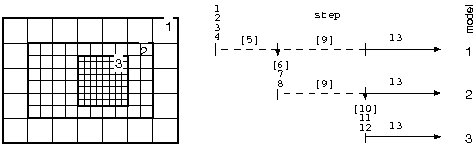
\includegraphics[width=15.cm]{annexes/seq1}
%\vspace*{-0.4cm}
\caption{Exemple of a grid-nesting simulation with 3 nested models
\label{seq1}}
\end{figure}
\newpage
\item The following initialisation and gridnesting sequence is shown here for
 three models, model~2 included in model~1, and model~3 included in model~1.
Model~3 has the same resolution as model~2 and is started after model~2
 to follow atmospheric system
(figure (\ref{seq2})):
\begin{enumerate}
\item
{\bf PREP\_PGD}: 
\begin{itemize}
\item one physiographic data file for the model 1 (definition of projection, resolution, domain)
\item one physiographic data file for the models 2 and 3 (same projection,
definition of resolution, domain)
\end{itemize} 
\item
{\bf PREP\_NEST\_PGD}: this program checks all the two PGD files at the same 
time, and imposes the conformity between them.
\item
{\bf extractecmwf} or {\bf extractarpege}: it extracts the surface
and altitude fields for one date, for model 1.
The extraction must be done separately for each date and time (for
the initial file and each of the coupling file of model~1).
\item 
{\bf PREP\_REAL\_CASE}: this program is run several times, for the initial
file and the coupling files of model~1.
\item 
{\bf MESONH}: this step is {\bf optional}. If you do not wish to start 
all the models at the same time, you can decide to run the model~1 before
the model~2 starts.
\item
{\bf ZOOM\_PGD}: Since the second PGD file was done for models
2 and 3, you have to zoom it on the domain of model~2 with this program.
\item
{\bf SPAWNING}: when you want to start the model~2, you must use this
program to compute the horizontal interpolations from the model 1 to the model
2. It is used only once for the initialisation of model~2.
\item 
{\bf PREP\_REAL\_CASE}: It is used only once, to compute the
initial file for the model~2. {\bf Do not change the vertical grid}.
\item 
{\bf MESONH}: here is your complete nested run with model~1 and model~2.
\item
{\bf ZOOM\_PGD}: Since the second PGD file was done for the models
2 and 3, you have to zoom it on the domain of model~3 with this program.
The domain of model~3 has a common zone with the one of model~2.
\item
{\bf SPAWNING}: when you want to start the model 3, you must use this
program to compute the horizontal interpolations from the model 1 and to 
use the fields of model 2 in the common domain.
It is used only once for the initialisation of model~3.
\item 
{\bf PREP\_REAL\_CASE}: It is used only once, to compute the
initial file for the model~3. {\bf Do not change the vertical grid}.
\item 
{\bf MESONH}: here is the nested run with model~1 and model~3.

\end{enumerate} 

\begin{figure}[htb]
\vspace*{1.cm}
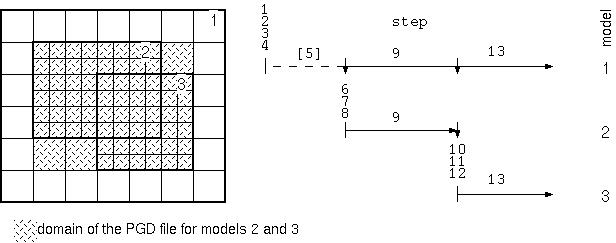
\includegraphics[width=15.cm]{annexes/seq2}
\caption{Exemple of a grid-nesting simulation with 3 nested models (the domain
of the 2 finest models has the same resolution and a common zone to follow
atmospheric system).
\label{seq2}}
\end{figure}
\end{itemize} 

\chapter{LES diagnostics} \label{s:LESdiag}

\section{Notations}

\begin{center}
\begin{tabular}{|l|l|l|}
\hline
$\alpha'$ & subgrid fluctuation of $\alpha$ &  \\
\hline
$\overline{\alpha}$ & mean value of $\alpha$ in the grid: resolved quantity & 3D \\
\hline
$<\alpha>$ &  horizontal mean value of $\alpha$ & 1D\\
\hline
$\tilde{\alpha} = \overline{\alpha}-<\alpha>$ &  resolved fluctuation 
to the mean profile & 3D\\
\hline
$<\alpha>_{up}$ &  horizontal mean value of $\alpha$ in updrafts;& 1D \\
& only point with $\overline{w}$ greater than $<w>$ are considered &\\
\hline
$<\alpha>_{down}$ &  horizontal mean value of $\alpha$ in downdrafts;& 1D \\
& only point with $\overline{w}$ smaller than $<w>$ are considered& \\
\hline
\end{tabular}
\end{center}


Examples:


\begin{center}
\begin{tabular}{|l|l|l|l|}
\hline
$\alpha'\beta'$ & & subgrid flux or (co)variance  $\alpha'\beta'$ & 3D \\
\hline
$\overline{\alpha}$  & & mean value of $\alpha$ in each grid mesh & 3D \\
\hline
$\overline{\alpha'}$  & $= 0$ & mean value of the turbulent fluctuation in each grid mesh & 3D \\
\hline
$\overline{\alpha'\beta'}$ & & mean value in each grid mesh of subgrid flux or (co)variance & 3D\\
\hline
$\tilde{\alpha}\,\tilde{\beta}$ & & resolved flux or (co)variance in each grid mesh & 3D\\
\hline
$<\alpha>$ & &  horizontal mean value of $\alpha$ & 1D \\
\hline
$<\alpha'>$ & $=0$ &  horizontal mean value of a subgrid fluctuation & 1D\\
\hline
$<\overline{\alpha}>$ & $= <\alpha>$ &  horizontal mean value of a resolved field& 1D\\
\hline
$<\tilde{\alpha}>$ & $= 0$ &  horizontal mean value of a resolved fluctuation& 1D\\
\hline
$<\overline{\alpha'\beta'}>$ & & horizontal mean value of subgrid flux or (co)variance & 1D\\
\hline
$<\tilde{\alpha}\,\tilde{\beta}>$ & & horizontal mean value of resolved flux or (co)variance & 1D\\
\hline
\end{tabular}
\end{center}


\section{What is available}

The computed fields have usually at least two
dimensions: z and t, that is they are temporal evolutions
of vertical profiles. They are always written in the 
diachronic file. Each field have its own group name,
say 'NAME'.

When time averaging is asked for, the fields are temporally
averaged (and so lose their temporal dimension) , and are written
under the name 'A\_NAME'.

When normalization is asked for, this one is made individually on
each vertical profile, for all times. They are written under
the name 'E\_NAME'.

When both normalization and time averaging are asked for,
normalization is made first, and then time averaging. The resulting
vertical profiles are written under the name 'H\_NAME'.\\

\section{LES averaged fields (LLES\_MEAN=TRUE)}


\begin{center}
\begin{makeimage}
\begin{tabular}{||p{6cm}|>{\centering}p{2.5cm}|>{\centering}p{1.5cm}|>{\centering}p{0.5cm}|p{5cm }||}
\hline
\hline
field & notation in the & dim. &   if  & comments \\
      & diachronic file & &  & \\
\hline
\hline
$<u>$ & MEAN\_U & z,t,p & &\multirow{15}{5cm}{dimension 'p' is equal to the  number of masks when this dimension is not present, the computation is made only on the cartesian mask.}\\
\cline{1-4}
$<v>$ & MEAN\_V &z,t,p &   &  \\
\cline{1-4}
$<w>$  & MEAN\_W &z,t,p &   & \\
\cline{1-4}
$<p>$   & MEAN\_PRE &z,t,p &   & \\
\cline{1-4}
$<\rho>$   & MEAN\_RHO &z,t,p &   & \\
\cline{1-4}
$<\theta>$   & MEAN\_TH &z,t,p &   &\\
\cline{1-4}
$<\theta_l>$   & MEAN\_THL &z,t,p &  $r_c$  &\\
\cline{1-4}
$<\theta_v>$   & MEAN\_THV &z,t,p &  $r_v$  &\\
\cline{1-4}
$<r_v>$   & MEAN\_RV &z,t,p &  $r_v$  &\\
\cline{1-4}
$<r_c>$   & MEAN\_RC &z,t,p &  $r_c$  &\\
\cline{1-4}
$<r_r>$   & MEAN\_RR &z,t,p &  $r_r$  &\\
\cline{1-4}
$<r_i>$   & MEAN\_RI &z,t,p &  $r_i$  &\\
\cline{1-4}
$<r_s>$   & MEAN\_RS &z,t,p &  $r_s$  &\\
\cline{1-4}
$<r_g>$   & MEAN\_RG &z,t,p &  $r_g$  &\\
\cline{1-4}
$<r_h>$   & MEAN\_RH &z,t,p &  $r_h$  &\\
\cline{1-4}
$<s_v>$   & MEAN\_SV &z,t,p,n &  $s_v$  &\\
\cline{1-4}
$<CLDFR>$   & MEAN\_CF &z,t,p,n &  $s_v$  &\\
\cline{1-4}
$<RAINFR>$   & MEAN\_RF &z,t,p,n &  $s_v$  &\\
\hline
$<\sqrt{\overline{u}^2+\overline{v}^2}>$   & MEAN\_WIND &z,t,p &   & different from $\sqrt{<\overline{u}>^2+<\overline{v}>^2}$ !\\
\hline
$<\overline{\rho} \;{\rm max}(\overline{w},<w>) >$  & MEAN\_MSFX &z,t,p &   & mean upward mass flux\\
\hline
\hline
\end{tabular}
\end{makeimage}
\end{center}

\newpage
\section{LES pdf (LLES\_PDF=TRUE)}

\begin{center}
\begin{makeimage}
\begin{tabular}{||p{6cm}|>{\centering}p{2.5cm}|>{\centering}p{1.5cm}|>{\centering}p{0.5cm}|p{5cm }||}
\hline
\hline
field & notation in the & dim. & if    & comments \\
      & diachronic file & &  & \\
\hline
\hline
$PDF\_\theta$ & PDF\_TH & z,t,p,n & &\multirow{11}{5cm}{dimension 'p' is equal to the  number of masks when this dimension is not present, the computation is made only on the cartesian mask.} \\
\cline{1-4}
$PDF\_W$ & PDF\_W &z,t,p,n &   &  \\
\cline{1-4}
$PDF\_\theta_v$ & PDF\_THV &z,t,p,n &   & \\
\cline{1-4}
$PDF\_R_v$ & PDF\_RV &z,t,p,n &   &  \\
\cline{1-4}
$PDF\_R_c$ & PDF\_RC &z,t,p,n &   &\\
\cline{1-4}
$PDF\_R_t$ & PDF\_RT &z,t,p,n &   &\\
\cline{1-4}
$PDF\_\theta_l$ & PDF\_THL &z,t,p,n &   &\\
\cline{1-4}
$PDF\_R_r$ & PDF\_RR &z,t,p,n &   &\\
\cline{1-4}
$PDF\_R_i$ & PDF\_RI &z,t,p,n &   &\\
\cline{1-4}
$PDF\_R_s$ & PDF\_RS &z,t,p,n &   &\\
\cline{1-4}
$PDF\_R_g$ & PDF\_RG &z,t,p,n &   &\\
\hline
\hline
\end{tabular}
\end{makeimage}
\end{center}

\section{LES averaged fields (LLES\_RESOLVED=TRUE)}

\begin{center}
\begin{makeimage}
\begin{tabular}{||p{6cm}|>{\centering}p{2.5cm}|>{\centering}p{1.5cm}|>{\centering}p{0.5cm}|p{5cm }||}
\hline
\hline
field & notation in the & dim. &if     & comments \\
      & diac. file &           &  & \\
\hline
\hline
$<\tilde{u}^2>$ & RES\_U2 & z,t,p & &\multirow{25}{5cm}{warning, contains both turbulent and gravity wave fields }\\
\cline{1-4}
$<\tilde{v}^2>$ & RES\_V2 &z,t,p &   & \\
\cline{1-4}
$<\tilde{w}^2>$ & RES\_W2 &z,t,p &   & \\
\cline{1-4}
$<\tilde{u}\;\tilde{v}>$ & RES\_UV &z,t,p &   &\\
\cline{1-4}
$<\tilde{w}\;\tilde{u}>$ & RES\_WU &z,t,p &   & \\
\cline{1-4}
$<\tilde{w}\;\tilde{v}>$ & RES\_WV &z,t,p &   &\\
\cline{1-4}
$<\frac{1}{2}(\tilde{u}^2+\tilde{v}^2+\tilde{w}^2)>$ & RES\_KE &z,t,p &   &\\
\cline{1-4}
$<\tilde{p}^2>$ & RES\_P2 & z,t,p &  & \\
\cline{1-4}
$<\tilde{u}\frac{\partial}{\partial z}\tilde{p}>$ & RES\_UPZ & z,t,p &  &\\
\cline{1-4}
$<\tilde{v}\frac{\partial}{\partial z}\tilde{p}>$ & RES\_VPZ & z,t,p &  &\\
\cline{1-4}
$<\tilde{w}\frac{\partial}{\partial z}\tilde{p}>$ & RES\_WPZ & z,t,p &  &\\
\cline{1-4}
$<\tilde{\theta}\;\tilde{\theta_v}>$ & RES\_THTV &z,t,p &  $r_v$  &\\
\cline{1-4}
$<\tilde{\theta_l}\;\tilde{\theta_v}>$ & RES\_TLTV &z,t,p &  $r_c$  &\\
\cline{1-4}
$<\tilde{\theta}^2>$ & RES\_TH2 &z,t,p &   &\\
\cline{1-4}
$<\tilde{\theta_l}^2>$ & RES\_THL2 &z,t,p &  $r_c$  &\\
\cline{1-4}
$<\tilde{u}\tilde{\theta}>$ & RES\_UTH &z,t,p &   & \\
\cline{1-4}
$<\tilde{v}\tilde{\theta}>$ & RES\_VTH &z,t,p &   &\\
\cline{1-4}
$<\tilde{w}\tilde{\theta}>$ & RES\_WTH &z,t,p &   &\\
\cline{1-4}
$<\tilde{u}\tilde{\theta_l}>$ & RES\_UTHL &z,t,p &  $r_c$  &\\
\cline{1-4}
$<\tilde{v}\tilde{\theta_l}>$ & RES\_VTHL &z,t,p &   $r_c$ &\\
\cline{1-4}
$<\tilde{w}\tilde{\theta_l}>$ & RES\_WTHL &z,t,p &   $r_c$ &\\
\cline{1-4}
$<\tilde{u}\tilde{\theta_v}>$ & RES\_UTHV &z,t,p &  $r_v$  &\\
\cline{1-4}
$<\tilde{v}\tilde{\theta_v}>$ & RES\_VTHV &z,t,p &   $r_v$ &\\
\cline{1-4}
$<\tilde{w}\tilde{\theta_v}>$ & RES\_WTHV &z,t,p &   $r_v$ &\\
\hline
\hline
\end{tabular}
\end{makeimage}
\end{center}
\begin{center}
\begin{makeimage}
\begin{tabular}{||p{6cm}|>{\centering}p{2.5cm}|>{\centering}p{1.5cm}|>{\centering}p{0.5cm}|p{5cm }||}
\hline
\hline
$<\tilde{r_v}^2>$ & RES\_RV2 &z,t,p &   $r_v$ &\multirow{25}{5cm}{warning, contains both turbulent and gravity wave fields }\\
\cline{1-4}
$<\tilde{\theta}\tilde{r_v}>$ & RES\_THRV &z,t,p &   $r_v$ &\\
\cline{1-4}
$<\tilde{\theta_l}\tilde{r_v}>$ & RES\_TLRV &z,t,p &   $r_c$ &\\
\cline{1-4}
$<\tilde{\theta_v}\tilde{r_v}>$ & RES\_TVRV &z,t,p &  $r_v$ &\\
\cline{1-4}
$<\tilde{u}\tilde{r_v}>$ & RES\_URV &z,t,p &  $r_v$  &\\
\cline{1-4}
$<\tilde{v}\tilde{r_v}>$ & RES\_VRV &z,t,p &   $r_v$ &\\
\cline{1-4}
$<\tilde{w}\tilde{r_v}>$ & RES\_WRV &z,t,p &   $r_v$ &\\
\cline{1-4}
$<\tilde{r_c}^2>$ & RES\_RC2 &z,t,p &   $r_c$ &\\
\cline{1-4}
$<\tilde{\theta}\tilde{r_c}>$ & RES\_THRC &z,t,p &   $r_c$ &\\
\cline{1-4}
$<\tilde{\theta_l}\tilde{r_c}>$ & RES\_TLRC &z,t,p &   $r_c$ &\\
\cline{1-4}
$<\tilde{\theta_v}\tilde{r_c}>$ & RES\_TVRC &z,t,p &   $r_c$ &\\
\cline{1-4}
$<\tilde{u}\tilde{r_c}>$ & RES\_URC &z,t,p &  $r_c$  &\\
\cline{1-4}
$<\tilde{v}\tilde{r_c}>$ & RES\_VRC &z,t,p &   $r_c$ &\\
\cline{1-4}
$<\tilde{w}\tilde{r_c}>$ & RES\_WRC &z,t,p &   $r_c$ &\\
\cline{1-4}
$<\tilde{r_i}^2>$ & RES\_RI2 &z,t,p &   $r_i$ &\\
\cline{1-4}
$<\tilde{\theta}\tilde{r_i}>$ & RES\_THRI &z,t,p &   $r_i$ &\\
\cline{1-4}
$<\tilde{\theta_l}\tilde{r_i}>$ & RES\_TLRI &z,t,p &   $r_i$ &\\
\cline{1-4}
$<\tilde{\theta_v}\tilde{r_i}>$ & RES\_TVRI &z,t,p &   $r_i$ &\\
\cline{1-4}
$<\tilde{u}\tilde{r_i}>$ & RES\_URI &z,t,p &  $r_i$  &\\
\cline{1-4}
$<\tilde{v}\tilde{r_i}>$ & RES\_VRI &z,t,p &   $r_i$ &\\
\cline{1-4}
$<\tilde{w}\tilde{r_i}>$ & RES\_WRI &z,t,p &   $r_i$ &\\
\cline{1-4}
$<\tilde{w}\tilde{r_r}>$ & RES\_WRR &z,t,p &   $r_r$ &\\
\cline{1-4}
Precipitation flux  & INPRR3D  &z,t,p &   $r_r$ &\\
\cline{1-4}
Max Precipitation flux  & MAXINPRR3D  &z,t,p &   $r_r$ &\\
\cline{1-4}
Evaporation flux  & EVAP3D  &z,t,p &   $r_r$ &\\
\cline{1-4}
$<\tilde{s_v}^2>$ & RES\_SV2 &z,t,p,n &   $s_v$ &\\
\cline{1-4}
$<\tilde{\theta}\tilde{s_v}>$ & RES\_THSV &z,t,p,n &   $s_v$ &\\
\cline{1-4}
$<\tilde{\theta_l}\tilde{s_v}>$ & RES\_TLSV &z,t,p,n &  $s_v$ &\\
\cline{1-4}
$<\tilde{\theta_v}\tilde{s_v}>$ & RES\_TVSV &z,t,p,n &  $s_v$ &\\
\cline{1-4}
$<\tilde{u}\tilde{s_v}>$ & RES\_USV &z,t,p,n  & $s_v$  &\\
\cline{1-4}
$<\tilde{v}\tilde{s_v}>$ & RES\_VSV &z,t,p,n  &  $s_v$ &\\
\cline{1-4}
$<\tilde{w}\tilde{s_v}>$ & RES\_WSV &z,t,p,n  &  $s_v$ &\\
\cline{1-4}
$<\tilde{w}^3>$ & RES\_W3 &z,t,p   &  $s_v$ &\\
\cline{1-4}
$<\tilde{w}\;\tilde{\theta_l}^2>$ & RES\_WTL2 &z,t,p &  $r_c$ &\\
\cline{1-4}
$<\tilde{w}^2\;\tilde{\theta_l}>$ & RES\_W2TL &z,t,p &  $r_c$ &\\
\cline{1-4}
$<\tilde{w}\;\tilde{r_t}^2>$ & RES\_WRT2 &z,t,p &  $r_c$ &\\
\cline{1-4}
$<\tilde{w}^2\;\tilde{r_t}>$ & RES\_W2RT &z,t,p &  $r_c$ &\\
\cline{1-4}
$<\tilde{w}\;\tilde{\theta_l};\tilde{r_t}>$ & RES\_WTLRT &z,t,p &  $r_c$ &\\
\cline{1-4}
$<\tilde{w}\;\tilde{r_v}^2>$ & RES\_WRV2 &z,t,p &  $r_v$ &\\
\cline{1-4}
$<\tilde{w}^2\;\tilde{r_v}>$ & RES\_W2RV &z,t,p &  $r_v$ &\\
\hline
$<\tilde{w}\;\tilde{\theta_l}\tilde{r_v}>$ & RES\_WTLRV &z,t,p &  $r_v$ &{if $r_v$ and no $r_c$, replaced by $<\tilde{w}\;\tilde{\theta}\tilde{r_v}>$}\\
\hline
$<\tilde{w}\;\tilde{r_c}^2>$ & RES\_WRC2 &z,t,p &  $r_c$ &\\
\cline{1-4}
$<\tilde{w}^2\;\tilde{r_c}>$ & RES\_W2RC &z,t,p &  $r_c$ &\\
\cline{1-4}
$<\tilde{w}\;\tilde{\theta_l}\tilde{r_c}>$ & RES\_WTLRC &z,t,p &  $r_c$ & \\
\cline{1-4}
$<\tilde{w}\;\tilde{r_v}\tilde{r_c}>$ & RE\_WRVRC &z,t,p &  $r_c$ &\\
\hline
\hline
\end{tabular}
\end{makeimage}
\end{center}

\begin{center}
\begin{tabular}{||p{6cm}|>{\centering}p{2.5cm}|>{\centering}p{1.5cm}|>{\centering}p{0.5cm}|p{5cm }||}
\hline
\hline
field & notation in & dim. &   if  & comments \\
      & diac. file &           &  & \\
\hline
\hline
$<\tilde{w}\;\tilde{r_i}^2>$ & RES\_WRI2 &z,t,p &  $r_i$ &\\
\cline{1-4}
$<\tilde{w}^2\;\tilde{r_i}>$ & RES\_W2RI &z,t,p &  $r_i$ &\\
\cline{1-4}
$<\tilde{w}\;\tilde{\theta_l}\tilde{r_i}>$ & RE\_WTLRI &z,t,p &  $r_i$ &\\
\cline{1-4}
$<\tilde{w}\;\tilde{r_v}\tilde{r_i}>$ & RE\_WRVRI &z,t,p &  $r_i$ & \\
\cline{1-4}
$<\tilde{w}\;\tilde{s_v}^2>$ & RES\_WSV2 &z,t,p,n &  $s_v$ &\\
\cline{1-4}
$<\tilde{w}^2\;\tilde{s_v}>$ & RES\_W2SV &z,t,p,n & $s_v$ &\\
\cline{1-5}
$<\tilde{w}\;\tilde{\theta_l}\tilde{s_v}>$ & RE\_WTLSV &z,t,p,n &  $s_v$ & if no $r_c$, replaced by \\
&&&&$<\tilde{w}\;\tilde{\theta}\tilde{s_v}>$ \\
\cline{1-5}
$<\tilde{w}\;\tilde{r_v}\tilde{s_v}>$ & RE\_WRVSV &z,t,p,n  & $r_v$, $s_v$ & \\
\cline{1-5}
$<\tilde{\theta_l}\frac{\partial}{\partial z}\tilde{p}>$ & RES\_TLPZ & z,t,p & & if no $r_c$, replaced by\\
&&&& $<\tilde{\theta}\frac{\partial}{\partial z,t,p}\tilde{p}>$ \\
\cline{1-5}
$<\tilde{r_v}\frac{\partial}{\partial z}\tilde{p}>$ & RES\_RVPZ & z,t,p & $r_v$  &\\
\cline{1-4}
$<\tilde{r_c}\frac{\partial}{\partial z}\tilde{p}>$ & RES\_RCPZ & z,t,p &  $r_c$  &\\
\cline{1-4}
$<\tilde{r_i}\frac{\partial}{\partial z}\tilde{p}>$ & RES\_RIPZ & z,t,p &  $r_i$  &\\
\cline{1-4}
$<\tilde{s_v}\frac{\partial}{\partial z}\tilde{p}>$ & RES\_SVPZ & z,t,p,n &  $s_v$  &\\
\cline{1-4}
$<\tilde{u}\left[\frac{1}{2}(\tilde{u}^2+\tilde{v}^2+\tilde{w}^2)\right]>$ & RES\_UKE & z,t,p &   &\\
\cline{1-4}
$<\tilde{v}\left[\frac{1}{2}(\tilde{u}^2+\tilde{v}^2+\tilde{w}^2)\right]>$ & RES\_VKE & z,t,p &   &\\
\cline{1-4}
$<\tilde{w}\left[\frac{1}{2}(\tilde{u}^2+\tilde{v}^2+\tilde{w}^2)\right]>$ & RES\_WKE & z,t,p &   &\\
\hline
\hline
\end{tabular}
\end{center}

\section{LES averaged fields (LLES\_SUBGRID=TRUE)}

\begin{center}
\begin{tabular}{||p{6cm}|>{\centering}p{2.5cm}|>{\centering}p{1.5cm}|>{\centering}p{0.5cm}|p{5cm }||}
\hline
\hline
field & notation in & dim. &   if  & comments \\
      & diac. file &           &  & \\
\hline
\hline
$<\frac{1}{2}(\overline{u'^2}+\overline{v'^2}+\overline{w'^2})>$ & SBG\_TKE &z,t,p &   & \\
\hline
$<\overline{u'^2}>$ & SBG\_U2 &z,t,p &   & \\
\hline
$<\overline{v'^2}>$ & SBG\_V2 &z,t,p &   & \\
\hline
$<\overline{w'^2}>$ & SBG\_W2 &z,t,p &   & \\
\hline
$<\overline{u'v'}>$ & SBG\_UV &z,t,p &   & \\
\hline
$<\overline{w'u'}>$ & SBG\_WU &z,t,p &   & \\
\hline
$<\overline{w'v'}>$ & SBG\_WV &z,t,p &   & \\
\hline
$<\overline{\theta_l'^2}>$ & SBG\_THL2 &z,t,p &   & if no $r_c$, replaced by $<\overline{\theta'^2}>$\\
\hline
$<\overline{u'\theta_l'}>$ & SBG\_UTHL &z,t,p &   & if no $r_c$, replaced by $<\overline{u'\theta'}>$ \\
\hline
$<\overline{v'\theta_l'}>$ & SBG\_VTHL &z,t,p &   & if no $r_c$, replaced by $<\overline{v'\theta'}>$ \\
\hline
$<\overline{w'\theta_l'}>$ & SBG\_WTHL &z,t,p &   & if no $r_c$, replaced by $<\overline{w'\theta'}>$ \\
\hline
\hline
\end{tabular}
\end{center}

\begin{center}
\begin{tabular}{||p{6cm}|>{\centering}p{2.5cm}|>{\centering}p{1.5cm}|>{\centering}p{0.5cm}|p{5cm }||}
\hline
\hline
$<\overline{w'\theta_v'}>$ & SBG\_WTHV &z,t,p & $r_v$  &  \\
\hline
$<\overline{r_t'^2}>$ & SBG\_RT2 &z,t,p & $r_v$  & $r_t$ is for total water \\
\hline
$<\overline{\theta_l'r_t'}>$ & SBG\_TLRT &z,t,p & $r_v$   & if no $r_c$, replaced by $<\overline{\theta'r_v'}>$ \\
\hline
$<\overline{u'r_t'}>$ & SBG\_URT &z,t,p & $r_v$  & $r_t$ is for total water\\
\hline
$<\overline{v'r_t'}>$ & SBG\_VRT &z,t,p & $r_v$  &$r_t$ is for total water \\
\hline
$<\overline{w'r_t'}>$ & SBG\_WRT &z,t,p & $r_v$  &$r_t$ is for total water \\
\hline
$<\overline{r_c'^2}>$ & SBG\_RC2 &z,t,p & $r_c$  & \\
\hline
$<\overline{u'r_c'}>$ & SBG\_URC &z,t,p & $r_c$  & \\
\hline
$<\overline{v'r_c'}>$ & SBG\_VRC &z,t,p & $r_c$  & \\
\hline
$<\overline{w'r_c'}>$ & SBG\_WRC &z,t,p & $r_c$  & \\
\hline
$<\overline{u's_v'}>$ & SBG\_USV &z,t,p,n & $s_v$  & \\
\hline
$<\overline{v's_v'}>$ & SBG\_VSV &z,t,p,n & $s_v$  & \\
\hline
$<\overline{w's_v'}>$ & SBG\_WSV &z,t,p,n & $s_v$  & \\
\hline
$<\overline{u'}\left[\frac{1}{2}(\overline{u'^2}+\overline{v'^2}+\overline{w'^2})\right]>$ & SBG\_UTKE & z,t,p &   &\\
\hline
$<\overline{v'}\left[\frac{1}{2}(\overline{u'^2}+\overline{v'^2}+\overline{w'^2})\right]>$ & SBG\_VTKE & z,t,p &   &\\
\hline
$<\overline{w'}\left[\frac{1}{2}(\overline{u'^2}+\overline{v'^2}+\overline{w'^2})\right]>$ & SBG\_WTKE & z,t,p &   &\\
\hline
$<\overline{\theta_l'}_{Updraft}>$ & SBG\_THLUP &z,t,p &   & \\
\hline
$<\overline{r_t'}_{Updraft}>$ & SBG\_RTUP &z,t,p & $r_v$  & \\
\hline
$<\overline{r_v'}_{Updraft}>$ & SBG\_RVUP &z,t,p & $r_v$  & \\
\hline
$<\overline{r_c'}_{Updraft}>$ & SBG\_RCUP &z,t,p & $r_c$  & \\
\hline
$<\overline{r_i'}_{Updraft}>$ & SBG\_RIUP &z,t,p & $r_i$  & \\
\hline
$<\overline{\theta_l}_{Updraft Mass Flux}>$ & THLUP\_MF &z,t,p & $r_i$  & \\
\hline
$<\overline{r_t}_{Updraft Mass Flux}>$ & RTUP\_MF &z,t,p & $r_v$  & \\
\hline
$<\overline{r_v}_{Updraft Mass Flux}>$ & RVUP\_MF &z,t,p & $r_v$  & \\
\hline
$<\overline{r_c}_{Updraft Mass Flux}>$ & RCUP\_MF &z,t,p & $r_c$  & \\
\hline
$<\overline{r_i}_{Updraft Mass Flux}>$ & RIUP\_MF &z,t,p & $r_i$  & \\
\hline
$<\overline{W}_{Updraft Mass Flux}>$ & WUP\_MF &z,t,p & $   $  & \\
\hline
$<\overline{Mass Flux}_{Updraft Mass Flux}>$ & MAFLX\_MF &z,t,p & $   $  & \\
\hline
$<\overline{Detr}_{Updraft Mass Flux}>$ & DETR\_MF &z,t,p & $   $  & \\
\hline
$<\overline{Entr}_{Updraft Mass Flux}>$ & ENTR\_MF &z,t,p & $   $  & \\
\hline
$<\overline{Frac}_{Updraft Mass Flux}>$ & FRCUP\_MF &z,t,p & $   $  & \\
\hline
$<\overline{\theta_v}_{Updraft Mass Flux}>$ & THVUP\_MF &z,t,p & $   $  & \\
\hline
$<\overline{w'\theta'_l}_{Mass Flux}>$ & WTHL\_MF &z,t,p & $   $  & \\
\hline
$<\overline{w'r'_t}_{Mass Flux}>$ & WRT\_MF &z,t,p & $   $  & \\
\hline
$<\overline{w'\theta'_v}_{Mass Flux}>$ & WTHV\_MF &z,t,p & $   $  & \\
\hline
$<\overline{w'u'}_{Mass Flux}>$ & WU\_MF &z,t,p & $   $  & \\
\hline
$<\overline{w'v'}_{Mass Flux}>$ & WV\_MF &z,t,p & $   $  & \\
\hline
\hline
\end{tabular}
\end{center}

\newpage

\section{LES averaged fields (LLES\_UPDRAFT=TRUE)}
\begin{center}
\begin{makeimage}
\begin{tabular}{||p{6cm}|>{\centering}p{2.5cm}|>{\centering}p{1.5cm}|>{\centering}p{0.9cm}|p{4.1cm }||}
\hline
\hline
%field & notation in the & dim. &     & comments \\
%      & diac. file &           & if & \\
%\hline
%\hline
$<f_{up}>$ & UP\_FRAC & z,t & & updraft fraction \\
\hline
$<w>_{up}$ & UP\_W & z,t & &\multirow{15}{4.1cm}{ from now, computations are made only on the cartesian mask}\\
\cline{1-4}
$<\theta>_{up}$& UP\_TH & z,t & & \\
\cline{1-4}
$<\theta_l>_{up}$& UP\_THL & z,t & $r_c$ & \\
\cline{1-4}
$<\theta_v>_{up}$& UP\_THV & z,t & $r_v$ & \\
\cline{1-4}
$<\frac{1}{2}(\tilde{u}^2+\tilde{v}^2+\tilde{w}^2)>_{up}$ & UP\_KE & z,t & & \\
\cline{1-4}
$<\frac{1}{2}(\tilde{u'^2}+\tilde{v'^2}+\tilde{w'^2})>_{up}$ & UP\_TKE & z,t & & \\
\cline{1-4}
$<r_v>_{up}$ & UP\_RV & z,t & $r_v$ & \\
\cline{1-4}
$<r_c>_{up}$& UP\_RC & z,t & $r_c$ & \\
\cline{1-4}
$<r_r>_{up}$& UP\_RR & z,t & $r_r$ & \\
\cline{1-4}
$<r_i>_{up}$ & UP\_RI & z,t & $r_i$ & \\
\cline{1-4}
$<r_s>_{up}$& UP\_RS & z,t & $r_s$ & \\
\cline{1-4}
$<r_g>_{up}$ & UP\_RG & z,t & $r_g$ & \\
\cline{1-4}
$<r_h>_{up}$ & UP\_RH & z,t & $r_h$ & \\
\cline{1-4}
$<s_v>_{up}$ & UP\_SV & z,t,n & $s_v$ & \\
\cline{1-4}
$<{\tilde{\theta}^2}>_{up}$ & UP\_TH2 & z,t &  & \\
\cline{1-4}
$<{\tilde{\theta_l}^2}>_{up}$& UP\_THL2 & z,t & $r_c$ & \\
\cline{1-4}
$<{\tilde{\theta}\;\tilde{\theta_v}}>_{up}$ & UP\_THTV & z,t & $r_v$ & \\
\cline{1-4}
$<{\tilde{\theta_l}\;\tilde{\theta_v}}>_{up}$ & UP\_TLTV & z,t & $r_c$ & \\
\cline{1-4}
$<{\tilde{w}\;\tilde{\theta}}>_{up}$ & UP\_WTH & z,t & & \\
\cline{1-4}
$<{\tilde{w}\;\tilde{\theta_l}}>_{up}$ & UP\_WTHL & z,t & $r_c$ & \\
\cline{1-4}
$<{\tilde{w}\;\tilde{\theta_v}}>_{up}$ & UP\_WTHV & z,t & $r_v$ & \\
\cline{1-4}
$<{\tilde{r_v}}^2>_{up}$ & UP\_RV2 & z,t & $r_v$ & \\
\cline{1-4}
$<{\tilde{\theta}\;\tilde{r_v}}>_{up}$ & UP\_THRV & z,t & $r_v$ & \\
\cline{1-4}
$<{\tilde{\theta_l}\;\tilde{r_v}}>_{up}$ & UP\_TLRV & z,t & $r_c$ & \\
\cline{1-4}
$<{\tilde{\theta_v}\;\tilde{r_v}}>_{up}$ & UP\_TVRV & z,t & $r_v$ & \\
\cline{1-4}
$<{\tilde{w}\;\tilde{r_v}}>_{up}$ & UP\_WRV & z,t & $r_v$ & \\
\cline{1-4}
$<{\tilde{r_c}}^2>_{up}$ & UP\_RC2 & z,t & $r_c$ & \\
\cline{1-4}
$<{\tilde{\theta}\;\tilde{r_c}}>_{up}$ & UP\_THRC & z,t & $r_c$ & \\
\cline{1-4}
$<{\tilde{\theta_l}\;\tilde{r_c}}>_{up}$ & UP\_TLRC & z,t & $r_c$ & \\
\cline{1-4}
$<{\tilde{\theta_v}\;\tilde{r_c}}>_{up}$ & UP\_TVRC & z,t & $r_c$ & \\
\cline{1-4}
$<{\tilde{w}\;\tilde{r_c}}>_{up}$ & UP\_WRC & z,t & $r_c$ & \\
\cline{1-4}
$<{\tilde{r_i}}^2>_{up}$ & UP\_RI2 & z,t & $r_i$ & \\
\cline{1-4}
$<{\tilde{\theta}\;\tilde{r_i}}>_{up}$ & UP\_THRI & z,t & $r_i$ & \\
\cline{1-4}
$<{\tilde{\theta_l}\;\tilde{r_i}}>_{up}$ & UP\_TLRI & z,t & $r_i$ & \\
\cline{1-4}
$<{\tilde{\theta_v}\;\tilde{r_i}}>_{up}$ & UP\_TVRI & z,t & $r_i$ & \\
\cline{1-4}
$<{\tilde{w}\;\tilde{r_i}}>_{up}$ & UP\_WRI & z,t & $r_i$ & \\
\cline{1-4}
$<{\tilde{s_v}}^2>_{up}$ & UP\_SV2 & z,t,n & $s_v$ & \\
\cline{1-4}
$<{\tilde{\theta}\;\tilde{s_v}}>_{up}$ & UP\_THSV & z,t,n & & \\
\cline{1-4}
$<{\tilde{\theta_l}\;\tilde{s_v}}>_{up}$ & UP\_TLSV & z,t,n & $r_c$, $s_v$ & \\
\cline{1-4}
$<{\tilde{\theta_v}\;\tilde{s_v}}>_{up}$& UP\_TVSV & z,t,n & $r_v$, $s_v$ & \\
\cline{1-4}
$<{\tilde{w}\;\tilde{s_v}}>_{up}$ & UP\_WSV & z,t,n & $s_v$ & \\
\hline
\hline
\end{tabular}
\end{makeimage}
\end{center}

\section{LES averaged fields (LLES\_DOWNDRAFT=TRUE)}

\begin{center}
\begin{tabular}{||p{6cm}|>{\centering}p{2.5cm}|>{\centering}p{1.5cm}|>{\centering}p{1cm}|p{4cm }||}
%\hline
%\hline
%field & notation in the & dim. &   if  & comments \\
%      & diac. file &           &  & \\
\hline
\hline
$<f_{dw}>$ & DW\_FRAC & z,t & & downdraft fraction \\
\hline
$<w>_{dw}$ & DW\_W & z,t & & \\
\hline
$<\theta>_{dw}$& DW\_TH & z,t & & \\
\hline
$<\theta_l>_{dw}$& DW\_THL & z,t & $r_c$ & \\
\hline
$<\theta_v>_{dw}$& DW\_THV & z,t & $r_v$ & \\
\hline
$<\frac{1}{2}(\tilde{u}^2+\tilde{v}^2+\tilde{w}^2)>_{dw}$ & DW\_KE & z,t & & \\
\hline
$<\frac{1}{2}(\tilde{u'^2}+\tilde{v'^2}+\tilde{w'^2})>_{dw}$ & DW\_TKE & z,t & & \\
\hline
$<r_v>_{dw}$ & DW\_RV & z,t & $r_v$ & \\
\hline
$<r_c>_{dw}$& DW\_RC & z,t & $r_c$ & \\
\hline
$<r_r>_{dw}$& DW\_RR & z,t & $r_r$ & \\
\hline
$<r_i>_{dw}$ & DW\_RI & z,t & $r_i$ & \\
\hline
$<r_s>_{dw}$& DW\_RS & z,t & $r_s$ & \\
\hline
$<r_g>_{dw}$ & DW\_RG & z,t & $r_g$ & \\
\hline
$<r_h>_{dw}$ & DW\_RH & z,t & $r_h$ & \\
\hline
$<s_v>_{dw}$ & DW\_SV & z,t,n & $s_v$ & \\
\hline
$<{\tilde{\theta}^2}>_{dw}$ & DW\_TH2 & z,t &  & \\
\hline
$<{\tilde{\theta_l}^2}>_{dw}$& DW\_THL2 & z,t & $r_c$ & \\
\hline
$<{\tilde{\theta}\;\tilde{\theta_v}}>_{dw}$ & DW\_THTV & z,t & $r_v$ & \\
\hline
$<{\tilde{\theta_l}\;\tilde{\theta_v}}>_{dw}$ & DW\_TLTV & z,t & $r_c$ & \\
\hline
$<{\tilde{w}\;\tilde{\theta}}>_{dw}$ & DW\_WTH & z,t & & \\
\hline
$<{\tilde{w}\;\tilde{\theta_l}}>_{dw}$ & DW\_WTHL & z,t & $r_c$ & \\
\hline
$<{\tilde{w}\;\tilde{\theta_v}}>_{dw}$ & DW\_WTHV & z,t & $r_v$ & \\
\hline
$<{\tilde{r_v}}^2>_{dw}$ & DW\_RV2 & z,t & $r_v$ & \\
\hline
$<{\tilde{\theta}\;\tilde{r_v}}>_{dw}$ & DW\_THRV & z,t & $r_v$ & \\
\hline
$<{\tilde{\theta_l}\;\tilde{r_v}}>_{dw}$ & DW\_TLRV & z,t & $r_c$ & \\
\hline
$<{\tilde{\theta_v}\;\tilde{r_v}}>_{dw}$ & DW\_TVRV & z,t & $r_v$ & \\
\hline
$<{\tilde{w}\;\tilde{r_v}}>_{dw}$ & DW\_WRV & z,t & $r_v$ & \\
\hline
$<{\tilde{r_c}}^2>_{dw}$ & DW\_RC2 & z,t & $r_c$ & \\
\hline
$<{\tilde{\theta}\;\tilde{r_c}}>_{dw}$ & DW\_THRC & z,t & $r_c$ & \\
\hline
$<{\tilde{\theta_l}\;\tilde{r_c}}>_{dw}$ & DW\_TLRC & z,t & $r_c$ & \\
\hline
$<{\tilde{\theta_v}\;\tilde{r_c}}>_{dw}$ & DW\_TVRC & z,t & $r_c$ & \\
\hline
$<{\tilde{w}\;\tilde{r_c}}>_{dw}$ & DW\_WRC & z,t & $r_c$ & \\
\hline
$<{\tilde{r_i}}^2>_{dw}$ & DW\_RI2 & z,t & $r_i$ & \\
\hline
$<{\tilde{\theta}\;\tilde{r_i}}>_{dw}$ & DW\_THRI & z,t & $r_i$ & \\
\hline
$<{\tilde{\theta_l}\;\tilde{r_i}}>_{dw}$ & DW\_TLRI & z,t & $r_i$ & \\
\hline
$<{\tilde{\theta_v}\;\tilde{r_i}}>_{dw}$ & DW\_TVRI & z,t & $r_i$ & \\
\hline
$<{\tilde{w}\;\tilde{r_i}}>_{dw}$ & DW\_WRI & z,t & $r_i$ & \\
\hline
$<{\tilde{s_v}}^2>_{dw}$ & DW\_SV2 & z,t,n & $s_v$ & \\
\hline
$<{\tilde{\theta}\;\tilde{s_v}}>_{dw}$ & DW\_THSV & z,t,n & & \\
\hline
$<{\tilde{\theta_l}\;\tilde{s_v}}>_{dw}$ & DW\_TLSV & z,t,n & $r_c$, $s_v$ & \\
\hline
$<{\tilde{\theta_v}\;\tilde{s_v}}>_{dw}$& DW\_TVSV & z,t,n & $r_v$, $s_v$ & \\
\hline
$<{\tilde{w}\;\tilde{s_v}}>_{dw}$ & DW\_WSV & z,t,n & $s_v$ & \\
\hline
\hline
\end{tabular}
\end{center}
\newpage
\section{LES averaged surface fields}

\begin{center}
\begin{tabular}{||p{6cm}|>{\centering}p{2.5cm}|>{\centering}p{1.5cm}|>{\centering}p{0.5cm}|p{5cm }||}
\hline
\hline
field & notation in & dimen- & if    & comments \\
      & diac. file &  sion         &  & \\
\hline
\hline
$<\overline{w'\theta'}_{surf}>$ & Q0 & t & & surface sensible flux \\
\hline
$<\overline{w'r_v'}_{surf}>$ & E0 & t & $r_v$  & surface latent flux  \\
\hline
$<\overline{w's_v'}_{surf}>$ & E0 & t,n & $s_v$  & surface scalar flux  \\
\hline
$u_*=\left\{<\overline{u'w'}_{surf}>^2+<\overline{v'w'}_{surf}>^2\right\}^\frac{1}{4}$ & U* & t &   & friction velocity  \\
\hline
$w_*=\left\{<\frac{g}{\theta}><\overline{w'\theta_v'}_{surf}><h>\right\}^\frac{1}{3}$ & W* & t &   & convective velocity \\
& & & & if positive surface  \\
& & & & buoyancy flux  \\
\hline
$<h>$ & BL\_H & t &  & boundary layer height  \\
\hline
$<L_{MO}>$ & L\_MO & t &  & Monin-Obukhov length  \\
\hline
$\int{TKE}dz$ & INT\_TKE & t &  & vertical integrated TKE  \\
\hline
 & ZCB & t &  & cloud base height  \\
\hline
$CF$ & ZCFTOT & t & $r_c$ & total cloud cover   \\
\hline
$\int{\rho (r_c+r_r)}$ & LWP & t & $r_c$ & Cloud water path  \\
\hline
$VAR_LWP$ & LWPVAR & t & $r_c$ & LWP variance  \\
\hline
$\int{\rho r_r}$ & RWP & t & $r_r$ & Rain water path  \\
\hline
$INPRR$ & INST\_PREC & t & $r_r$ & Inst. precip. rate  \\
\hline
 & RAIN\_PREC & t & $r_r$ & INPRR over rainy grids  \\
\hline
$ACPRR$ & ACCU\_PREC & t & $r_r$ & Accum. precip. rate  \\
\hline
$H_CFmax$ & ZMAXCF & t & $r_c$ & Height of cloud fraction maximum  \\
\hline
\hline
\end{tabular}
\end{center}

\section{Other LES averaged fields}

\begin{center}
\begin{tabular}{||p{6cm}|>{\centering}p{2.5cm}|>{\centering}p{1.5cm}|>{\centering}p{0.5cm}|p{5cm }||}
\hline
\hline
field & notation in & dimen- & if    & comments \\
      & diac. file &  sion         &  & \\
\hline
\hline
$sw_{up}$ & SWU & z,t,p & & SW upward radiative flux  \\
\hline
$sw_{down}$ & SWD & z,t,p & & SW downward radiative flux  \\
\hline
$lw_{up}$ & LWU & z,t,p & & LW upward radiative flux  \\
\hline
$lw_{down}$ & LWD & z,t,p & & LW downward radiative flux  \\
\hline
$dthrad_{sw}$ & DTHRADSW & z,t,p & & SW radiative temperature tendency  \\
\hline
$dthrad_{lw}$ & DTHRADLW & z,t,p & & LW radiative temperature tendency  \\
\hline
Mean Effective Radius & RADEFF & z,t,p & & Mean effective radius  \\
\hline
\hline
\end{tabular}
\end{center}
\newpage
\section{LES 2 points correlations}
\begin{center}
\begin{tabular}{||p{6cm}|>{\centering}p{2.5cm}|>{\centering}p{1.5cm}|>{\centering}p{0.5cm}|p{5cm }||}
\hline
\hline
field & notation in the & dim. &  if  & comments\\
& diac. file &           &  & \\
\hline
\hline
$<\tilde{u}(x,y)\;\tilde{u}(x+l_x,y)>$ & CI\_UU & $l_x$,2,z,t & & \\
\hline
$<\tilde{u}(x,y)\;\tilde{u}(x,y+l_y)>$ & CJ\_UU & $l_y$,2,z,t & & \\
\hline
$<\tilde{v}(x,y)\;\tilde{v}(x+l_x,y)>$ & CI\_VV & $l_x$,2,z,t & & \\
\hline
$<\tilde{v}(x,y)\;\tilde{v}(x,y+l_y)>$ & CJ\_VV & $l_y$,2,z,t & & \\
\hline
$<\tilde{w}(x,y)\;\tilde{w}(x+l_x,y)>$ & CI\_WW & $l_x$,2,z,t & & \\
\hline
$<\tilde{w}(x,y)\;\tilde{w}(x,y+l_y)>$ & CJ\_WW & $l_y$,2,z,t & & \\
\hline
$<\tilde{u}(x,y)\;\tilde{v}(x+l_x,y)>$ & CI\_UV & $l_x$,2,z,t & & \\
\hline
$<\tilde{u}(x,y)\;\tilde{v}(x,y+l_y)>$ & CJ\_UV & $l_y$,2,z,t & & \\
\hline
$<\tilde{w}(x,y)\;\tilde{u}(x+l_x,y)>$ & CI\_WU & $l_x$,2,z,t & & \\
\hline
$<\tilde{w}(x,y)\;\tilde{u}(x,y+l_y)>$ & CJ\_WV & $l_y$,2,z,t & & \\
\hline
$<\tilde{\theta}(x,y)\;\tilde{\theta}(x+l_x,y)>$ & CI\_THTH & $l_x$,2,z,t & & \\
\hline
$<\tilde{\theta}(x,y)\;\tilde{\theta}(x,y+l_y)>$ & CJ\_THTH & $l_y$,2,z,t & & \\
\hline
$<\tilde{\theta_l}(x,y)\;\tilde{\theta_l}(x+l_x,y)>$ & CI\_TLTL & $l_x$,2,z,t & $r_c$ & \\
\hline
$<\tilde{\theta_l}(x,y)\;\tilde{\theta_l}(x,y+l_y)>$ & CJ\_TLTL & $l_y$,2,z,t &  $r_c$& \\
\hline
$<\tilde{w}(x,y)\;\tilde{\theta}(x+l_x,y)>$ & CI\_WTH & $l_x$,2,z,t & & \\
\hline
$<\tilde{w}(x,y)\;\tilde{\theta}(x,y+l_y)>$ & CJ\_WTH & $l_y$,2,z,t & & \\
\hline
$<\tilde{w}(x,y)\;\tilde{\theta_l}(x+l_x,y)>$ & CI\_WTHL & $l_x$,2,z,t & $r_c$ & \\
\hline
$<\tilde{w}(x,y)\;\tilde{\theta_l}(x,y+l_y)>$ & CJ\_WTHL & $l_y$,2,z,t & $r_c$ & \\
\hline
$<\tilde{r_v}(x,y)\;\tilde{r_v}(x+l_x,y)>$ & CI\_RVRV & $l_x$,2,z,t & $r_v$ & \\
\hline
$<\tilde{r_v}(x,y)\;\tilde{r_v}(x,y+l_y)>$ & CJ\_RVRV & $l_y$,2,z,t & $r_v$ & \\
\hline
$<\tilde{\theta}(x,y)\;\tilde{r_v}(x+l_x,y)>$ & CI\_THRV & $l_x$,2,z,t & $r_v$ & \\
\hline
$<\tilde{\theta}(x,y)\;\tilde{r_v}(x,y+l_y)>$ & CJ\_THRV & $l_y$,2,z,t & $r_v$ & \\
\hline
$<\tilde{\theta_l}(x,y)\;\tilde{r_v}(x+l_x,y)>$ & CI\_TLRV & $l_x$,2,z,t & $r_c$ & \\
\hline
$<\tilde{\theta_l}(x,y)\;\tilde{r_v}(x,y+l_y)>$ & CJ\_TLRV & $l_y$,2,z,t & $r_c$ & \\
\hline
$<\tilde{w}(x,y)\;\tilde{r_v}(x+l_x,y)>$ & CI\_WRV & $l_x$,2,z,t & $r_v$ & \\
\hline
$<\tilde{w}(x,y)\;\tilde{r_v}(x,y+l_y)>$ & CJ\_WRV & $l_y$,2,z,t & $r_v$ & \\
\hline
$<\tilde{r_c}(x,y)\;\tilde{r_c}(x+l_x,y)>$ & CI\_RCRC & $l_x$,2,z,t & $r_c$ & \\
\hline
$<\tilde{r_c}(x,y)\;\tilde{r_c}(x,y+l_y)>$ & CJ\_RCRC & $l_y$,2,z,t & $r_c$ & \\
\hline
$<\tilde{\theta}(x,y)\;\tilde{r_c}(x+l_x,y)>$ & CI\_THRC & $l_x$,2,z,t & $r_c$ & \\
\hline
$<\tilde{\theta}(x,y)\;\tilde{r_c}(x,y+l_y)>$ & CJ\_THRC & $l_y$,2,z,t & $r_c$ & \\
\hline
$<\tilde{\theta_l}(x,y)\;\tilde{r_c}(x+l_x,y)>$ & CI\_TLRC & $l_x$,2,z,t & $r_c$ & \\
\hline
$<\tilde{\theta_l}(x,y)\;\tilde{r_c}(x,y+l_y)>$ & CJ\_TLRC & $l_y$,2,z,t & $r_c$ & \\
\hline
$<\tilde{w}(x,y)\;\tilde{r_c}(x+l_x,y)>$ & CI\_WRC & $l_x$,2,z,t & $r_c$ & \\
\hline
$<\tilde{w}(x,y)\;\tilde{r_c}(x,y+l_y)>$ & CJ\_WRC & $l_y$,2,z,t & $r_c$ & \\
\hline
$<\tilde{r_i}(x,y)\;\tilde{r_i}(x+l_x,y)>$ & CI\_RIRI & $l_x$,2,z,t & $r_i$ & \\
\hline
$<\tilde{r_i}(x,y)\;\tilde{r_i}(x,y+l_y)>$ & CJ\_RIRI & $l_y$,2,z,t & $r_i$ & \\
\hline
$<\tilde{\theta}(x,y)\;\tilde{r_i}(x+l_x,y)>$ & CI\_THRI & $l_x$,2,z,t & $r_i$ & \\
\hline
$<\tilde{\theta}(x,y)\;\tilde{r_i}(x,y+l_y)>$ & CJ\_THRI & $l_y$,2,z,t & $r_i$ & \\
\hline
$<\tilde{\theta_l}(x,y)\;\tilde{r_i}(x+l_x,y)>$ & CI\_TLRI & $l_x$,2,z,t & $r_i$ & \\
\hline
$<\tilde{\theta_l}(x,y)\;\tilde{r_i}(x,y+l_y)>$ & CJ\_TLRI & $l_y$,2,z,t & $r_i$ & \\
\hline
\hline
\end{tabular}
\end{center}
\begin{center}
\begin{tabular}{||p{6cm}|>{\centering}p{2.5cm}|>{\centering}p{1.5cm}|>{\centering}p{0.5cm}|p{5cm }||}
\hline
\hline
field & notation in the & dim. &  if  & comments\\
& diac. file &           &  & \\
\hline
\hline
$<\tilde{w}(x,y)\;\tilde{r_i}(x+l_x,y)>$ & CI\_WRI & $l_x$,2,z,t & $r_i$ & \\
\hline
$<\tilde{w}(x,y)\;\tilde{r_i}(x,y+l_y)>$ & CJ\_WRI & $l_y$,2,z,t & $r_i$ & \\
\hline
$<\tilde{s_v}(x,y)\;\tilde{s_v}(x+l_x,y)>$ & CI\_SVSV & $l_x$,2,z,t,n & $s_v$ & \\
\hline
$<\tilde{s_v}(x,y)\;\tilde{s_v}(x,y+l_y)>$ & CJ\_SVSV & $l_y$,2,z,t,n & $s_v$ & \\
\hline
$<\tilde{w}(x,y)\;\tilde{s_v}(x+l_x,y)>$ & CI\_WSV & $l_x$,2,z,t,n & $s_v$ & \\
\hline
$<\tilde{w}(x,y)\;\tilde{s_v}(x,y+l_y)>$ & CJ\_WSV & $l_y$,2,z,t,n & $s_v$ & \\
\hline
\hline
\end{tabular}
\end{center}

\section{LES spectra}
\begin{center}
\begin{makeimage}
\begin{tabular}{||p{6cm}|>{\centering}p{2.5cm}|>{\centering}p{1.5cm}|>{\centering}p{0.5cm}|p{5cm }||}
\hline
\hline
field & notation in the & dim. &  if  & comments\\
& diac. file &           &  & \\
\hline
\hline
$\frac{1}{2\pi L}\int_L<\tilde{u}(x,y)\;\tilde{u}(x+l_x,y)>\;e^{-ik_xl_x}dl_x$ & SI\_UU & $k_x$,2,z,t & &\multirow{30}{5cm}{ dimension 2 is for real and imaginary parts}\\
\cline{1-4}
$\frac{1}{2\pi L}\int_L<\tilde{u}(x,y)\;\tilde{u}(x,y+l_y)>\;e^{-ik_yl_y}dl_y$ & SJ\_UU & $k_y$,2,z,t & & \\
\cline{1-4}
$\frac{1}{2\pi L}\int_L<\tilde{v}(x,y)\;\tilde{v}(x+l_x,y)>\;e^{-ik_xl_x}dl_x$ & SI\_VV & $k_x$,2,z,t & & \\
\cline{1-4}
$\frac{1}{2\pi L}\int_L<\tilde{v}(x,y)\;\tilde{v}(x,y+l_y)>\;e^{-ik_yl_y}dl_y$ & SJ\_VV & $k_y$,2,z,t & & \\
\cline{1-4}
$\frac{1}{2\pi L}\int_L<\tilde{w}(x,y)\;\tilde{w}(x+l_x,y)>\;e^{-ik_xl_x}dl_x$ & SI\_WW & $k_x$,2,z,t & & \\
\cline{1-4}
$\frac{1}{2\pi L}\int_L<\tilde{w}(x,y)\;\tilde{w}(x,y+l_y)>\;e^{-ik_yl_y}dl_y$ & SJ\_WW & $k_y$,2,z,t & & \\
\cline{1-4}
$\frac{1}{2\pi L}\int_L<\tilde{u}(x,y)\;\tilde{v}(x+l_x,y)>\;e^{-ik_xl_x}dl_x$ & SI\_UV & $k_x$,2,z,t & & \\
\cline{1-4}
$\frac{1}{2\pi L}\int_L<\tilde{u}(x,y)\;\tilde{v}(x,y+l_y)>\;e^{-ik_yl_y}dl_y$ & SJ\_UV & $k_y$,2,z,t & & \\
\cline{1-4}
$\frac{1}{2\pi L}\int_L<\tilde{w}(x,y)\;\tilde{u}(x+l_x,y)>\;e^{-ik_xl_x}dl_x$ & SI\_WU & $k_x$,2,z,t & & \\
\cline{1-4}
$\frac{1}{2\pi L}\int_L<\tilde{w}(x,y)\;\tilde{u}(x,y+l_y)>\;e^{-ik_yl_y}dl_y$ & SJ\_WV & $k_y$,2,z,t & & \\
\cline{1-4}
$\frac{1}{2\pi L}\int_L<\tilde{\theta}(x,y)\;\tilde{\theta}(x+l_x,y)>\;e^{-ik_xl_x}dl_x$ & SI\_THTH & $k_x$,2,z,t & & \\
\cline{1-4}
$\frac{1}{2\pi L}\int_L<\tilde{\theta}(x,y)\;\tilde{\theta}(x,y+l_y)>\;e^{-ik_yl_y}dl_y$ & SJ\_THTH & $k_y$,2,z,t & & \\
\cline{1-4}
$\frac{1}{2\pi L}\int_L<\tilde{\theta_l}(x,y)\;\tilde{\theta_l}(x+l_x,y)>\;e^{-ik_xl_x}dl_x$ & SI\_TLTL & $k_x$,2,z,t & $r_c$ & \\
\cline{1-4}
$\frac{1}{2\pi L}\int_L<\tilde{\theta_l}(x,y)\;\tilde{\theta_l}(x,y+l_y)>\;e^{-ik_yl_y}dl_y$ & SJ\_TLTL & $k_y$,2,z,t &  $r_c$ & \\
\cline{1-4}
$\frac{1}{2\pi L}\int_L<\tilde{w}(x,y)\;\tilde{\theta}(x+l_x,y)>\;e^{-ik_xl_x}dl_x$ & SI\_WTH & $k_x$,2,z,t & & \\
\hline
\hline
\end{tabular}
\end{makeimage}
\end{center}
\begin{center}
\begin{makeimage}
\begin{tabular}{||p{6cm}|>{\centering}p{2.5cm}|>{\centering}p{1.5cm}|>{\centering}p{0.5cm}|p{5cm }||}
\hline
\hline
field & notation in the & dim. &  if  & comments\\
& diac. file &           &  & \\
\hline
\hline

$\frac{1}{2\pi L}\int_L<\tilde{w}(x,y)\;\tilde{\theta}(x,y+l_y)>\;e^{-ik_yl_y}dl_y$ & SJ\_WTH & $k_y$,2,z,t & &\multirow{46}{5cm}{ dimension 2 is for real and imaginary parts} \\
\cline{1-4}
$\frac{1}{2\pi L}\int_L<\tilde{w}(x,y)\;\tilde{\theta_l}(x+l_x,y)>\;e^{-ik_xl_x}dl_x$ & SI\_WTHL & $k_x$,2,z,t & $r_c$ & \\
\cline{1-4}
$\frac{1}{2\pi L}\int_L<\tilde{w}(x,y)\;\tilde{\theta_l}(x,y+l_y)>\;e^{-ik_yl_y}dl_y$ & SJ\_WTHL & $k_y$,2,z,t & $r_c$ & \\
\cline{1-4}
$\frac{1}{2\pi L}\int_L<\tilde{r_v}(x,y)\;\tilde{r_v}(x+l_x,y)>\;e^{-ik_xl_x}dl_x$ & SI\_RVRV & $k_x$,2,z,t & $r_v$ & \\
\cline{1-4}
$\frac{1}{2\pi L}\int_L<\tilde{r_v}(x,y)\;\tilde{r_v}(x,y+l_y)>\;e^{-ik_yl_y}dl_y$ & SJ\_RVRV & $k_y$,2,z,t & $r_v$ & \\
\cline{1-4}
$\frac{1}{2\pi L}\int_L<\tilde{\theta}(x,y)\;\tilde{r_v}(x+l_x,y)>\;e^{-ik_xl_x}dl_x$ & SI\_THRV & $k_x$,2,z,t & $r_v$ & \\
\cline{1-4}
$\frac{1}{2\pi L}\int_L<\tilde{\theta}(x,y)\;\tilde{r_v}(x,y+l_y)>\;e^{-ik_yl_y}dl_y$ & SJ\_THRV & $k_y$,2,z,t & $r_v$ & \\
\cline{1-4}
$\frac{1}{2\pi L}\int_L<\tilde{\theta_l}(x,y)\;\tilde{r_v}(x+l_x,y)>\;e^{-ik_xl_x}dl_x$ & SI\_TLRV & $k_x$,2,z,t & $r_c$ & \\
\cline{1-4}
$\frac{1}{2\pi L}\int_L<\tilde{\theta_l}(x,y)\;\tilde{r_v}(x,y+l_y)>\;e^{-ik_yl_y}dl_y$ & SJ\_TLRV & $k_y$,2,z,t & $r_c$ & \\
\cline{1-4}
$\frac{1}{2\pi L}\int_L<\tilde{w}(x,y)\;\tilde{r_v}(x+l_x,y)>\;e^{-ik_xl_x}dl_x$ & SI\_WRV & $k_x$,2,z,t & $r_v$ & \\
\cline{1-4}
$\frac{1}{2\pi L}\int_L<\tilde{w}(x,y)\;\tilde{r_v}(x,y+l_y)>\;e^{-ik_yl_y}dl_y$ & SJ\_WRV & $k_y$,2,z,t & $r_v$ & \\
\cline{1-4}
$\frac{1}{2\pi L}\int_L<\tilde{r_c}(x,y)\;\tilde{r_c}(x+l_x,y)>\;e^{-ik_xl_x}dl_x$ & SI\_RCRC & $k_x$,2,z,t & $r_c$ & \\
\cline{1-4}
$\frac{1}{2\pi L}\int_L<\tilde{r_c}(x,y)\;\tilde{r_c}(x,y+l_y)>\;e^{-ik_yl_y}dl_y$ & SJ\_RCRC & $k_y$,2,z,t & $r_c$ & \\
\cline{1-4}
$\frac{1}{2\pi L}\int_L<\tilde{\theta}(x,y)\;\tilde{r_c}(x+l_x,y)>\;e^{-ik_xl_x}dl_x$ & SI\_THRC & $k_x$,2,z,t & $r_c$ & \\
\cline{1-4}
$\frac{1}{2\pi L}\int_L<\tilde{\theta}(x,y)\;\tilde{r_c}(x,y+l_y)>\;e^{-ik_yl_y}dl_y$ & SJ\_THRC & $k_y$,2,z,t & $r_c$ & \\
\cline{1-4}
$\frac{1}{2\pi L}\int_L<\tilde{\theta_l}(x,y)\;\tilde{r_c}(x+l_x,y)>\;e^{-ik_xl_x}dl_x$ & SI\_TLRC & $k_x$,2,z,t & $r_c$ & \\
\cline{1-4}
$\frac{1}{2\pi L}\int_L<\tilde{\theta_l}(x,y)\;\tilde{r_c}(x,y+l_y)>\;e^{-ik_yl_y}dl_y$ & SJ\_TLRC & $k_y$,2,z,t & $r_c$ & \\
\cline{1-4}
$\frac{1}{2\pi L}\int_L<\tilde{w}(x,y)\;\tilde{r_c}(x+l_x,y)>\;e^{-ik_xl_x}dl_x$ & SI\_WRC & $k_x$,2,z,t & $r_c$ & \\
\cline{1-4}
$\frac{1}{2\pi L}\int_L<\tilde{w}(x,y)\;\tilde{r_c}(x,y+l_y)>\;e^{-ik_yl_y}dl_y$ & SJ\_WRC & $k_y$,2,z,t & $r_c$ & \\
\cline{1-4}
$\frac{1}{2\pi L}\int_L<\tilde{r_i}(x,y)\;\tilde{r_i}(x+l_x,y)>\;e^{-ik_xl_x}dl_x$ & SI\_RIRI & $k_x$,2,z,t & $r_i$ & \\
\cline{1-4}
$\frac{1}{2\pi L}\int_L<\tilde{r_i}(x,y)\;\tilde{r_i}(x,y+l_y)>\;e^{-ik_yl_y}dl_y$ & SJ\_RIRI & $k_y$,2,z,t & $r_i$ & \\
\cline{1-4}
$\frac{1}{2\pi L}\int_L<\tilde{\theta}(x,y)\;\tilde{r_i}(x+l_x,y)>\;e^{-ik_xl_x}dl_x$ & SI\_THRI & $k_x$,2,z,t & $r_i$ & \\
\cline{1-4}
$\frac{1}{2\pi L}\int_L<\tilde{\theta}(x,y)\;\tilde{r_i}(x,y+l_y)>\;e^{-ik_yl_y}dl_y$ & SJ\_THRI & $k_y$,2,z,t & $r_i$ & \\
\hline
\hline
\end{tabular}
\end{makeimage}
\end{center}

\begin{center}
\begin{makeimage}
\begin{tabular}{||p{6cm}|>{\centering}p{2.5cm}|>{\centering}p{1.5cm}|>{\centering}p{0.5cm}|p{5cm }||}
\hline
\hline
field & notation in the & dim. &  if  & comments\\
& diac. file &           &  & \\
\hline
\hline
$\frac{1}{2\pi L}\int_L<\tilde{\theta_l}(x,y)\;\tilde{r_i}(x+l_x,y)>\;e^{-ik_xl_x}dl_x$ & SI\_TLRI & $k_x$,2,z,t & $r_i$ &\multirow{16}{5cm}{ dimension 2 is for real and imaginary parts} \\
\cline{1-4}
$\frac{1}{2\pi L}\int_L<\tilde{\theta_l}(x,y)\;\tilde{r_i}(x,y+l_y)>\;e^{-ik_yl_y}dl_y$ & SJ\_TLRI & $k_y$,2,z,t & $r_i$ & \\
\cline{1-4}
$\frac{1}{2\pi L}\int_L<\tilde{w}(x,y)\;\tilde{r_i}(x+l_x,y)>\;e^{-ik_xl_x}dl_x$ & SI\_WRI & $k_x$,2,z,t & $r_i$ & \\
\cline{1-4}
$\frac{1}{2\pi L}\int_L<\tilde{w}(x,y)\;\tilde{r_i}(x,y+l_y)>\;e^{-ik_yl_y}dl_y$ & SJ\_WRI & $k_y$,2,z,t & $r_i$ & \\
\cline{1-4}
$\frac{1}{2\pi L}\int_L<\tilde{s_v}(x,y)\;\tilde{s_v}(x+l_x,y)>\;e^{-ik_xl_x}dl_x$ & SI\_SVSV & $k_x$,2,z,t,n & $s_v$ & \\
\cline{1-4}
$\frac{1}{2\pi L}\int_L<\tilde{s_v}(x,y)\;\tilde{s_v}(x,y+l_y)>\;e^{-ik_yl_y}dl_y$ & SJ\_SVSV & $k_y$,2,z,t,n & $s_v$ & \\
\cline{1-4}
$\frac{1}{2\pi L}\int_L<\tilde{w}(x,y)\;\tilde{s_v}(x+l_x,y)>\;e^{-ik_xl_x}dl_x$ & SI\_WSV & $k_x$,2,z,t,n & $s_v$ & \\
\cline{1-4}
$\frac{1}{2\pi L}\int_L<\tilde{w}(x,y)\;\tilde{s_v}(x,y+l_y)>\;e^{-ik_yl_y}dl_y$ & SJ\_WSV & $k_y$,2,z,t,n & $s_v$ & \\
\hline
\hline
\end{tabular}
\end{makeimage}
\end{center}
%%%%%%%%%%%%%%%%%%%%%%%%%%%%%%%%%%%%%%%%%%%%%%%%%%%%%%%%%%%%%%%%%%%%%%%%%%%%%%%%%%%%%%%%%%%%%%%%
%%%%%%%%%%%%%%%%%%%%%%%%%%%%%%%%%%%%%%%%%%%%%%%%%%%%%%%%%%%%%%%%%%%%%%%%%%%%%%%%%%%%%%%%%%%%%%%%
%%%%%%%%%%%%%%%%%%%%%%%%%%%%%%%%%%%%%%%%%%%%%%%%%%%%%%%%%%%%%%%%%%%%%%%%%%%%%%%%%%%%%%%%%%%%%%%%
%%%%%%%%%%%%%%%%%%%%%%%%%%%%%%%%%%%%%%%%%%%%%%%%%%%%%%%%%%%%%%%%%%%%%%%%%%%%%%%%%%%%%%%%%%%%%%%%
\newpage
\section{Budget of (resolved + subgrid) turbulent quantities}

\subsection{Budget of total turbulent kinetic energy}


All terms of the equation of $\frac{\partial}{\partial t} (E+e)$ are
computed and stored in the diachronic group BU\_KE. Here, e and E
denote the subgrid and resolved Tke respectively:

\begin{displaymath}
<e>=<\frac{1}{2}(\overline{u'^2}+\overline{v'^2}+\overline{w'^2})> \hspace*{2.cm}
<E>=<\frac{1}{2}(\tilde{u}^2+\tilde{v}^2+\tilde{w}^2)>
\end{displaymath}


Here are {\bf main terms} of the equations for the horizontal mean
of subgrid Tke and resolved Tke, in the
frame of Boussinesq approximation. Note that the computations of the budgets terms are done with the complete equation set and discretization of MESONH.
The equations here are simplified only for the sake of easier
understanding.
Other terms can arise
from the parametrizations of MESONH, and will also be taken into account
in the budget.

\begin{displaymath}
\begin{array}{rllll}
\frac{\partial }{\partial t} <e> = & 
\overbrace{- <u_\alpha>\frac{\partial}{\partial x_\alpha} <e> }^{ADVM} &
\overbrace{- <\tilde{u_\alpha}\frac{\partial}{\partial x_\alpha} e > }^{ADVR} &
\overbrace{- \frac{1}{<\rho>}<\overline{u'_\alpha \frac{\partial p'}{\partial x_\alpha}}>}^{PRES} &
\overbrace{- <\frac{\partial}{\partial x_\alpha} \overline{u'_\alpha e}>}^{TR}\\
\vspace*{1.2cm}
&\underbrace{- <\overline{u'_\alpha u'_\beta}> \frac{\partial {<u_\beta>}}{\partial x_\alpha}}_{DPM} &
\underbrace{- <\overline{u'_\alpha u'_\beta} \frac{\partial {\tilde{u_\beta}}}{\partial x_\alpha}>}_{DPR} &
+ \underbrace{<\beta  \overline{w'\theta'_v}>}_{TP} & 
\underbrace{- <\epsilon>}_{DISS}\\
\end{array}
\end{displaymath}
\begin{displaymath}
\begin{array}{rllll}
\frac{\partial }{\partial t} <E> = & 
\overbrace{- <u_\alpha>\frac{\partial}{\partial x_\alpha} <E> }^{ADV} &
\overbrace{- \frac{1}{<\rho>}<\tilde{u_\alpha} \frac{\partial \tilde{p}}{\partial x_\alpha}>}^{PRES} &
\overbrace{- <\tilde{u_\alpha} \tilde{u_\beta}> \frac{\partial {<u_\beta>}}{\partial x_\alpha}}^{DP} &\\
&+ \underbrace{<\beta  \tilde{w}\tilde{\theta_v}>}_{TP} &
 \underbrace{- \frac{\partial}{\partial x_\alpha} <\tilde{u_\alpha} E>}_{TR} &
\underbrace{- <\tilde{u_\alpha}\frac{\partial}{\partial x_\beta}\overline{u'_\alpha u'_\beta}>}_{SBGT}  &+ ...
\end{array}
\end{displaymath}


The terms of (spectral) transport from resolved to subgrid motions is
SBTG in the equation of $<E>$ (sink), and
ADVR and DPR in the equation of $<e>$ (sources).
One should note that: \\

\begin{displaymath}
{\rm ADVR}+{\rm DPR} = -{\rm SGBT}
\end{displaymath}

\underline{Note in case of gridnesting}\\

In case of 2way gridnesting, the subgrid scheme is not alone to influence
the resolved motions due to subgrid scale. Part of the job is done
by the averaged of the smaller-scale models. 
The terms of (spectral) transport from resolved to subgrid motions are
then both SBTG and NEST in the equation of $<E>$ (sinks).
Therefore

\begin{displaymath}
{\rm ADVR}+\hat{\rm DPR} = -({\rm SGBT+NEST})
\end{displaymath}

Where $\hat{\rm DPR}$ is the dynamical production that should produce
the subgrid-scale model to equilibrate the sink at resolved scale.\\



\begin{center}
\begin{tabular}{||p{5cm}|>{\centering}p{2cm}|>{\centering}p{2.5cm}|>{\centering}p{0.5cm}|p{5.5cm }||}
\hline
\hline
field & notation in diac. file& processus name& dim.  & comments \\
\hline
\hline
$-\frac{\partial }{\partial t}<e>$ & BU\_KE & SBG TEND & z,t & (opposite of) tendency of $<e>$\\
\hline
$-<\overline{u'w'}>\frac{\partial }{\partial z}<u>$ & BU\_KE & SBG DP M & z,t & dyn. prod. by mean gradients \\
$-<\overline{v'w'}>\frac{\partial }{\partial z}<v>$ &  & &  & \\
\hline
$<-\overline{u'_\alpha u'_\beta}\frac{\partial}{\partial x_\beta}\tilde{u_\alpha}>$ & BU\_KE & SBG DP R & z,t & dyn. prod. by resolved \\
 & & & & fluctuations \\
\hline
$-<w>\frac{\partial}{\partial z}<e>$ & BU\_KE & SBG ADVM & z,t & advection \\
 & & & & by mean flow\\
\hline
$-<\tilde{u_\alpha}\frac{\partial}{\partial x_\alpha}e>$ & BU\_KE & SBG ADVR & z,t & advection by\\
 & & & &resolved flow\\
\hline
$-W_{forc}\frac{\partial}{\partial z}<e>$ & BU\_KE & SBG FORC & z,t & advection \\
 & & & & by large-scale\\
 & & & & W forcing\\
\hline
$-<\frac{\partial}{\partial z}\overline{w'e}>$ & BU\_KE & SBG TR   & z,t & subgrid turbulent transport\\
\hline
$- \frac{1}{<\rho>}<\overline{u'_\alpha \frac{\partial p'}{\partial x_\alpha}}>$&
BU\_KE & SBG PRES & z,t & subgrid pressure-\\
 & & & & correlation term\\
\hline
$<\beta  \overline{w'\theta'_v}>$ & BU\_KE & SBG TP   & z,t & thermal production \\
\hline
$-<\epsilon>$ & BU\_KE & SBG DISS & z,t & dissipation \\
\hline
{\rm numerical diffusion of } $<e>$& BU\_KE & SBG NUMD & z,t & numerical diffusion\\
 & & & &against $2\Delta x$ \\
\hline
{\rm relaxation of }$<e>$ & BU\_KE & SBG RELA & z,t& sponge layer relaxation \\
\hline
{\rm miscellaneous} & BU\_KE & SBG MISC & z,t & ... \\
\hline
{\rm residual of budget of} $<e>$ & BU\_KE & SBG RESI & z,t & must be zero \\
\hline
$-\frac{\partial }{\partial t}<E>$ & BU\_KE & RES TEND & z,t & (opposite of) tendency\\
 & & & &  of $<E>$\\
\hline
$-<w>\frac{\partial}{\partial z}<E>$ & BU\_KE & RES ADV  & z,t & advection \\
 & & & & by mean flow\\
\hline
$-W_{forc}\frac{\partial}{\partial z}<E>$ & BU\_KE & RES FORC & z,t & advection \\
 & & & & by large-scale\\
 & & & & W forcing\\
\hline
$-<\tilde{u}\tilde{w}>\frac{\partial }{\partial z}<u>$ & BU\_KE & RES DP   & z,t & dyn. prod. \\
 & & & &(by mean gradients)\\
$-<\tilde{v}\tilde{w}>\frac{\partial }{\partial z}<v>$ &  &  & & \\
\hline
$-\frac{\partial}{\partial x_\alpha} <\tilde{u_\alpha} E>$ & BU\_KE & RES TR   & z,t & transport of resolved Tke\\
 & & & &by itself \\
\hline
$- \frac{1}{<\rho>}<\tilde{u_\alpha} \frac{\partial \tilde{p}}{\partial x_\alpha}>$ & BU\_KE & RES PRES & z,t & pressure-correlations \\
\hline
$ <\beta  \tilde{w}\tilde{\theta_v}> $  & BU\_KE & RES TP   & z,t & thermal production \\
\hline
$- <\tilde{u_\alpha}\frac{\partial}{\partial x_\beta}\overline{u'_\alpha u'_\beta}> $ & BU\_KE & RES SBGT & z,t & sink due \\
 & & & &to subgrid turbulence \\
\hline
\hline
\end{tabular}
\end{center}

\begin{center}
\begin{tabular}{||p{5cm}|>{\centering}p{2cm}|>{\centering}p{2.5cm}|>{\centering}p{0.5cm}|p{5.5cm }||}
\hline
\hline
field & notation in diac. file& processus name& dim.  & comments \\
\hline
\hline
{\rm Coriolis terms} & BU\_KE & RES CORI & z,t & should be zero for $<E>$ \\
\hline
{\rm numerical diffusion of } $<E>$& BU\_KE & RES NUMD & z,t & numerical diffusion\\
 & & & &against $2\Delta x$ \\
\hline
{\rm relaxation of }$<E>$ & BU\_KE & RES RELA & z,t& sponge layer relaxation \\
\hline
{\rm 2way nesting of }$<E>$ & BU\_KE & RES NEST & z,t& average from smaller\\
 & & & &nested models \\
\hline
{\rm miscellaneous} & BU\_KE & RES MISC & z,t & curvature terms, ... \\
\hline
{\rm residual of budget of} $<E>$ & BU\_KE & RES RESI & z,t & must be zero \\
\hline
\hline
\end{tabular}
\end{center}


Note that if a term is zero, because the process accounting for it is
not activated in the model, the term is not listed in the diachronic file.
So, in order to know which terms have been computed and stored, use
the command 'print BU\_KE proc' in diaprog.\\ 

\subsection{Budget of total (liquid) temperature flux}

All terms of the equation of $\frac{\partial}{\partial t} (<\tilde{w}\tilde{\theta_l}> + <\overline{w'\theta_l'}>)$ are
computed and stored in the diachronic group BU\_WTHL. 
All comments made for the total Tke equation are valid here.\\

\begin{displaymath}
\left.
\begin{array}{rllll}
\frac{\partial }{\partial t} <\overline{w'\theta_l'}> = & 
\overbrace{- <u_\alpha>\frac{\partial}{\partial x_\alpha} <\overline{w'\theta_l'}> }^{ADVM} \;\;
\overbrace{- <\tilde{u_\alpha}\frac{\partial}{\partial x_\alpha} \overline{w'\theta_l'} > }^{ADVR} &
\overbrace{- <\overline{u_\alpha'w'}> \frac{\partial {<\theta_l>}}{\partial x_\alpha}
- <\overline{u'_\alpha \theta_l'}> \frac{\partial {<w>}}{\partial x_\alpha}}^{DPM} \\
\vspace*{1.0cm}
& \underbrace{- <\overline{u'_\alpha w'} \frac{\partial {\tilde{\theta_l}}}{\partial x_\alpha}>
- <\overline{u'_\alpha \theta_l'} \frac{\partial {\tilde{w}}}{\partial x_\alpha}>}_{DPR} \;\;
+ \underbrace{<\beta  \overline{\theta_l'\theta'_v}>}_{TP} &
\underbrace{- \frac{1}{<\rho>}<\overline{\theta_l' \frac{\partial p'}{\partial z}}>}_{PRES} \;\;\;\;\;\;\;
 \underbrace{- <\frac{\partial}{\partial x_\alpha} \overline{u'_\alpha w'\theta_l'}>}_{TR} \\
\frac{\partial }{\partial t} <\tilde{w}\tilde{\theta_l}> = & 
\overbrace{- <u_\alpha>\frac{\partial}{\partial x_\alpha} <\tilde{w}\tilde{\theta_l}> }^{ADV} \;\;
\overbrace{- \frac{1}{<\rho>}<\tilde{\theta_l} \frac{\partial \tilde{p}}{\partial x_\alpha}>}^{PRES} &
\overbrace{- <\tilde{u_\alpha} \tilde{w}> \frac{\partial {<\theta_l>}}{\partial x_\alpha}
- <\tilde{u_\alpha} \tilde{\theta_l}> \frac{\partial {<w>}}{\partial x_\alpha}}^{DP} &\\
&+ \underbrace{<\beta  \tilde{\theta_l}\tilde{\theta_v}>}_{TP} \;\;\;\;\;\;\;\;
 \underbrace{- \frac{\partial}{\partial x_\alpha} <\tilde{u_\alpha} \tilde{w}\tilde{\theta_l}>}_{TR} &
\underbrace{- <\tilde{w}\frac{\partial}{\partial x_\alpha}\overline{u'_\alpha \theta_l'}>
- <\tilde{\theta_l}\frac{\partial}{\partial x_\alpha}\overline{u'_\alpha w'}>}_{SBGT}\hspace{0.2cm} + ...&
\end{array}
\right.
\end{displaymath}

\begin{center}
\begin{tabular}{||p{5cm}|>{\centering}p{2cm}|>{\centering}p{2.5cm}|>{\centering}p{0.5cm}|p{5.5cm }||}
\hline
\hline
field & notation in diac. file & processus name& dim.  & comments \\
\hline
\hline
$-<\overline{w'^2}>\frac{\partial }{\partial z}<\theta_l>$ & BU\_WTHL & SBG DP M & z,t & dyn. prod. by mean gradient \\
\hline
$<-\overline{w'^2}\frac{\partial}{\partial z}\tilde{\theta_l}>$ & BU\_WTHL & SBG DP R & z,t & dyn. prod. by resolved\\
 & & & & fluctuations\\
\hline
$-<\frac{\partial}{\partial z}\overline{w'^2\theta_l'}>$ & BU\_WTHL & SBG TR   & z,t & subgrid turbulent transport\\
\hline
$- \frac{1}{<\rho>}<\overline{\theta_l' \frac{\partial p'}{\partial z}}>$&
BU\_WTHL & SBG PRES & z,t & subgrid pressure-\\
 & & & &correlation term \\
\hline
$<\beta  \overline{\theta_l'\theta'_v}>$ & BU\_WTHL & SBG TP   & z,t & thermal production \\
\hline
{\rm residual of budget of} $<\overline{w'\theta_l'}>$ & BU\_WTHL & SBG RESI & z,t & must be small \\
\hline
$-\frac{\partial }{\partial t}<\tilde{w}\tilde{\theta_l}>$ & BU\_WTHL & RES TEND & z,t & (opposite of) tendency\\
 & & & &of $<\tilde{w}\tilde{\theta_l}>$\\
\hline
$-<w>\frac{\partial}{\partial z}<\tilde{w}\tilde{\theta_l}>$ & BU\_WTHL & RES ADV  & z,t & advection \\
 & & & & by mean flow\\
\hline
$-W_{forc}\frac{\partial}{\partial z}<\tilde{w}\tilde{\theta_l}>$ & BU\_WTHL & RES FORC & z,t & advection \\
 & & & & by large-scale\\
 & & & & W forcing\\
\hline
$-<\tilde{w}^2>\frac{\partial }{\partial z}<\theta_l>$ & BU\_WTHL & RES DP   & z,t & dyn. prod.\\
 & & & &(by mean gradients) \\
$-<\tilde{w}\tilde{\theta_l}>\frac{\partial }{\partial z}<w>$ &  &  & & \\
\hline
$-\frac{\partial}{\partial x_\alpha} <\tilde{u_\alpha} \tilde{w}\tilde{\theta_l}>$ & BU\_WTHL & RES TR   & z,t & transport of resolved \\
 & & & & flux by itself \\
\hline
$- \frac{1}{<\rho>}<\tilde{\theta_l} \frac{\partial \tilde{p}}{\partial z}>$ & BU\_WTHL & RES PRES & z,t & pressure-correlations \\
\hline
$ <\beta  \tilde{\theta_l}\tilde{\theta_v}> $  & BU\_WTHL & RES TP   & z,t & thermal production \\
\hline
$- <\tilde{w}\frac{\partial}{\partial x_\alpha}\overline{u'_\alpha \theta_l'}>$
& BU\_WTHL & RES SBGT & z,t & sink due to\\
 & & & & subgrid turbulence \\
$- <\tilde{\theta_l}\frac{\partial}{\partial x_\alpha}\overline{u'_\alpha w'}>$
&&&&\\
\hline
{\rm Coriolis terms} & BU\_WTHL & RES CORI & z,t & \\
\hline
{\rm numerical diffusion of } $<\tilde{w}\tilde{\theta_l}>$& BU\_WTHL & RES NUMD & z,t & numerical diffusion\\
 & & & &against $2\Delta x$ \\
\hline
{\rm relaxation of }$<\tilde{w}\tilde{\theta_l}>$ & BU\_WTHL & RES RELA & z,t& sponge layer relaxation \\
\hline
{\rm 2way nesting of }$<\tilde{w}\tilde{\theta_l}>$ & BU\_WTHL & RES NEST & z,t& average from smaller \\
 & & & & nested models \\
\hline
{\rm miscellaneous} & BU\_WTHL & RES MISC & z,t & ref. pressure term,\\
 & & & & curvature term,\\
 & & & & microphysics,\\
 & & & & radiation, ...\\
\hline
{\rm residual of budget of} $<\tilde{w}\tilde{\theta_l}>$ & BU\_WTHL & RES RESI & z,t & must be zero \\
\hline
\hline
\end{tabular}
\end{center}

\begin{center}
\begin{tabular}{||p{5cm}|>{\centering}p{2cm}|>{\centering}p{2.5cm}|>{\centering}p{0.5cm}|p{5.5cm }||}
\hline
\hline
field & notation in diac. file & processus name& dim.  & comments \\
\hline
\hline
$-\frac{\partial }{\partial t}<\overline{w'\theta_l'}>$ & BU\_WTHL & NSG TEND & z,t & (neglected) opposite of\\
(neglected in turb. scheme) & & & &tendency\\
 & & & &of $<\overline{w'\theta_l'}>$ \\
\hline
$-<w>\frac{\partial}{\partial z}<\overline{w'\theta_l'}>$  & BU\_WTHL & NSG ADVM & z,t & (neglected) advection \\
 & & & & by mean flow\\
\hline
$-<\tilde{u_\alpha}\frac{\partial}{\partial x_\alpha}\overline{w'\theta_l'}>$  & BU\_WTHL & NSG ADVR & z,t & (neglected) advection\\
 & & & & by resolved flow\\
\hline
terms due to $\overline{w}$ gradients  & BU\_WTHL & NSG DPGW & z,t & (neglected) dyn. prod. terms \\
\hline
terms due to hor. $\overline{\theta_l}$ gradients  & BU\_WTHL & NSG DPGT & z,t & other (neglected)\\
 & & & & dyn. prod. terms\\
\hline
\hline
\end{tabular}
\end{center}


\subsection{Budget of total (liquid) temperature variance}


All terms of the equation of $\frac{\partial}{\partial t} (<\tilde{\theta_l}^2> + <\overline{\theta_l'^2}>)$ are
computed and stored in the diachronic group BU\_THL2. 
All comments made for the total Tke equation are valid here.\\

\begin{displaymath}
\left.
\begin{array}{rllll}
\frac{\partial }{\partial t} <\overline{\theta_l'^2}> = & 
\overbrace{- <u_\alpha>\frac{\partial}{\partial x_\alpha} <\overline{\theta_l'^2}> }^{ADVM}  &
\overbrace{- <\tilde{u_\alpha}\frac{\partial}{\partial x_\alpha} \overline{\theta_l'^2} > }^{ADVR} &
\overbrace{- 2 <\overline{u_\alpha'\theta_l'}> \frac{\partial {<\theta_l>}}{\partial x_\alpha} }^{DPM} \\
\vspace*{1.0cm}
& \underbrace{- 2 <\overline{u'_\alpha \theta_l'} \frac{\partial {\tilde{\theta_l}}}{\partial x_\alpha}>}_{DPR}  &
 \underbrace{- <\frac{\partial}{\partial x_\alpha} \overline{u'_\alpha \theta_l'^2}>}_{TR}
 & \underbrace{-\; \epsilon_{\theta}}_{DISS}\\
\frac{\partial }{\partial t} <\tilde{\theta_l}^2> = & 
\overbrace{- <u_\alpha>\frac{\partial}{\partial x_\alpha} <\tilde{\theta_l}^2> }^{ADV} &
\overbrace{- 2<\tilde{u_\alpha} \tilde{\theta_l}> \frac{\partial {<\theta_l>}}{\partial x_\alpha}}^{DP} &\\
& \underbrace{- \frac{\partial}{\partial x_\alpha} <\tilde{u_\alpha} \tilde{\theta_l}^2>}_{TR} &
\underbrace{- 2 <\tilde{\theta_l}\frac{\partial}{\partial x_\alpha}\overline{u'_\alpha \theta_l'}>}_{SBGT} & + ...
\end{array}
\right.
\end{displaymath}

\begin{center}
\begin{tabular}{||p{5cm}|>{\centering}p{2cm}|>{\centering}p{2.5cm}|>{\centering}p{0.5cm}|p{5.5cm }||}
\hline
\hline
field & notation in & processus & dim.  & comments \\
      & diac. file & name      &            & \\
\hline
\hline
$- 2 <\overline{w'\theta_l'}>\frac{\partial }{\partial z}<\theta_l>$ & BU\_THL2 & SBG DP M & z,t & dyn. prod. by mean gradient \\
\hline
$<-2 \overline{w'\theta_l'}\frac{\partial}{\partial z}\tilde{\theta_l}>$ & BU\_THL2 & SBG DP R & z,t & dyn. prod. by resolved fluctuations\\
\hline
$-<\frac{\partial}{\partial z}\overline{w'\theta_l'^2}>$ & BU\_THL2 & SBG TR   & z,t & subgrid turbulent transport\\
\hline
$-<\epsilon_\theta>$ & BU\_THL2 & SBG DISS & z,t & dissipation \\
\hline
{\rm residual of budget of} $<\overline{w'\theta_l'}>$ & BU\_THL2 & SBG RESI & z,t & must be small \\
\hline
\hline
\end{tabular}
\end{center}

\begin{center}
\begin{tabular}{||p{5cm}|>{\centering}p{2cm}|>{\centering}p{2.5cm}|>{\centering}p{0.5cm}|p{5.5cm }||}
\hline
\hline
field & notation in diac. file & processus name& dim.  & comments \\
\hline
\hline
$-\frac{\partial }{\partial t}<\tilde{\theta_l}^2>$ & BU\_THL2 & RES TEND & z,t & (opposite of) tendency\\
 & & & &of $<\tilde{\theta_l}^2>$\\
\hline
$-<w>\frac{\partial}{\partial z}<\tilde{\theta_l}^2>$ & BU\_THL2 & RES ADV  & z,t & advection by mean flow \\
\hline
$-W_{forc}\frac{\partial}{\partial z}<\tilde{\theta_l}^2>$ & BU\_THL2 & RES FORC & z,t & advection by \\
 & & & & large-scale W forcing \\
\hline
$-< 2 \tilde{w}\tilde{\theta_l}>\frac{\partial }{\partial z}<\theta_l>$ & BU\_THL2 & RES DP   & z,t & dyn. prod.\\
 & & & &(by mean gradients) \\
\hline
$-\frac{\partial}{\partial x_\alpha} <\tilde{u_\alpha} \tilde{\theta_l}^2>$ & BU\_THL2 & RES TR   & z,t & resolved transport of\\
 & & & &resolved variance \\
\hline
$- <2 \tilde{\theta_l}\frac{\partial}{\partial x_\alpha}\overline{u'_\alpha \theta_l'}>$
& BU\_THL2 & RES SBGT & z,t & sink due \\
 & & & &to subgrid turbulence \\
\hline
{\rm numerical diffusion of } $<\tilde{\theta_l}^2>$& BU\_THL2 & RES NUMD & z,t & numerical diffusion\\
 & & & &against $2\Delta x$ \\
\hline
{\rm relaxation of }$<\tilde{\theta_l}^2>$ & BU\_THL2 & RES RELA & z,t& sponge layer relaxation \\
\hline
{\rm 2way nesting of }$<\tilde{\theta_l}^2>$ & BU\_THL2 & RES NEST & z,t& average from smaller\\
 & & & &nested models \\
\hline
{\rm miscellaneous} & BU\_THL2 & RES MISC & z,t & ref. pressure term, \\
 & & && radiation, microphysics, ... \\
\hline
{\rm residual of budget of} $<\tilde{\theta_l}^2>$ & BU\_THL2 & RES RESI & z,t & must be zero \\
\hline
$-\frac{\partial }{\partial t}<\overline{\theta_l'^2}>$ & BU\_THL2 & NSG TEND & z,t & (neglected) opposite of\\
(neglected in turb. scheme) & & & &tendency of $<\overline{\theta_l'^2}>$ \\
\hline
$-<w>\frac{\partial}{\partial z}<\overline{\theta_l'^2}>$  & BU\_THL2 & NSG ADVM & z,t & (neglected) advection \\
 & & & & by mean flow\\
\hline
$-<\tilde{u_\alpha}\frac{\partial}{\partial x_\alpha}\overline{\theta_l'^2}>$  & BU\_THL2 & NSG ADVR & z,t & (neglected) advection by\\
 & & & &resolved flow\\
\hline
\hline
\end{tabular}
\end{center}
\newpage
\subsection{Budget of total water flux}


All terms of the equation of $\frac{\partial}{\partial t} (<\tilde{w}\tilde{r_t}> + <\overline{w'r_t'}>)$ are
computed and stored in the diachronic group BU\_WRT. 
All comments made for the total Tke equation are valid here.\\

\begin{displaymath}
\left.
\begin{array}{rllll}
\frac{\partial }{\partial t} <\overline{w'r_t'}> = & 
\overbrace{- <u_\alpha>\frac{\partial}{\partial x_\alpha} <\overline{w'r_t'}> }^{ADVM} \;\;
\overbrace{- <\tilde{u_\alpha}\frac{\partial}{\partial x_\alpha} \overline{w'r_t'} > }^{ADVR} &
\overbrace{- <\overline{u_\alpha'w'}> \frac{\partial {<r_t>}}{\partial x_\alpha}
- <\overline{u'_\alpha r_t'}> \frac{\partial {<w>}}{\partial x_\alpha}}^{DPM} \\
\vspace*{1.0cm}
& \underbrace{- <\overline{u'_\alpha w'} \frac{\partial {\tilde{r_t}}}{\partial x_\alpha}>
- <\overline{u'_\alpha r_t'} \frac{\partial {\tilde{w}}}{\partial x_\alpha}>}_{DPR} \;\;
+ \underbrace{<\beta  \overline{r_t'\theta'_v}>}_{TP} &
\underbrace{- \frac{1}{<\rho>}<\overline{r_t' \frac{\partial p'}{\partial z}}>}_{PRES} \;\;\;\;\;\;\;
 \underbrace{- <\frac{\partial}{\partial x_\alpha} \overline{u'_\alpha w'r_t'}>}_{TR} \\
\frac{\partial }{\partial t} <\tilde{w}\tilde{r_t}> = & 
\overbrace{- <u_\alpha>\frac{\partial}{\partial x_\alpha} <\tilde{w}\tilde{r_t}> }^{ADV} \;\;
\overbrace{- \frac{1}{<\rho>}<\tilde{r_t} \frac{\partial \tilde{p}}{\partial x_\alpha}>}^{PRES} &
\overbrace{- <\tilde{u_\alpha} \tilde{w}> \frac{\partial {<r_t>}}{\partial x_\alpha}
- <\tilde{u_\alpha} \tilde{r_t}> \frac{\partial {<w>}}{\partial x_\alpha}}^{DP} &\\
&+ \underbrace{<\beta  \tilde{r_t}\tilde{\theta_v}>}_{TP} \;\;\;\;\;\;\;\;
 \underbrace{- \frac{\partial}{\partial x_\alpha} <\tilde{u_\alpha} \tilde{w}\tilde{r_t}>}_{TR} &
\underbrace{- <\tilde{w}\frac{\partial}{\partial x_\alpha}\overline{u'_\alpha r_t'}>
- <\tilde{r_t}\frac{\partial}{\partial x_\alpha}\overline{u'_\alpha w'}>}_{SBGT}  + ...&
\end{array}
\right.
\end{displaymath}

\begin{center}
\begin{tabular}{||p{5cm}|>{\centering}p{2cm}|>{\centering}p{2.5cm}|>{\centering}p{0.5cm}|p{5.5cm }||}
\hline
\hline
field & notation in diac. file & processus name& dim.  & comments \\
\hline
\hline
$-<\overline{w'^2}>\frac{\partial }{\partial z}<r_t>$ & BU\_WRT & SBG DP M & z,t & dyn. prod. by mean gradient \\
\hline
$<-\overline{w'^2}\frac{\partial}{\partial z}\tilde{r_t}>$ & BU\_WRT & SBG DP R & z,t & dyn. prod. by resolved fluctuations\\
\hline
$-<\frac{\partial}{\partial z}\overline{w'^2r_t'}>$ & BU\_WRT & SBG TR   & z,t & subgrid turbulent transport\\
\hline
$- \frac{1}{<\rho>}<\overline{r_t' \frac{\partial p'}{\partial z}}>$&
BU\_WRT & SBG PRES & z,t & subgrid pressure-\\
 & & & &correlation term \\
\hline
$<\beta  \overline{r_t'\theta'_v}>$ & BU\_WRT & SBG TP   & z,t & thermal production \\
\hline
{\rm residual of budget of} $<\overline{w'r_t'}>$ & BU\_WRT & SBG RESI & z,t & must be small \\
\hline
%\hline
%\end{tabular}
%\end{center}
%
%\begin{center}
%\begin{tabular}{||p{5cm}|>{\centering}p{2cm}|>{\centering}p{2.5cm}|>{\centering}p{0.5cm}|p{5.5cm }||}
%\hline
%\hline
%field & notation in diac. file & processus name& dim.  & comments \\
%\hline
%\hline
$-\frac{\partial }{\partial t}<\tilde{w}\tilde{r_t}>$ & BU\_WRT & RES TEND & z,t & (opposite of) tendency\\
 & & & &of $<\tilde{w}\tilde{r_t}>$\\
\hline
$-<w>\frac{\partial}{\partial z}<\tilde{w}\tilde{r_t}>$ & BU\_WRT & RES ADV  & z,t & advection \\
 & & & & by mean flow\\
\hline
$-W_{forc}\frac{\partial}{\partial z}<\tilde{w}\tilde{r_t}>$ & BU\_WRT & RES FORC & z,t & advection \\
 & & & & by large-scale \\
 & & & & W forcing\\
\hline
$-<\tilde{w}^2>\frac{\partial }{\partial z}<r_t>$ & BU\_WRT & RES DP   & z,t & dyn. prod.\\
 & & & &(by mean gradients) \\
$-<\tilde{w}\tilde{r_t}>\frac{\partial }{\partial z}<w>$ &  &  & & \\
\hline
$-\frac{\partial}{\partial x_\alpha} <\tilde{u_\alpha} \tilde{w}\tilde{r_t}>$ & BU\_WRT & RES TR   & z,t & transport of resolved\\
 & & & &flux by itself \\
\hline
$- \frac{1}{<\rho>}<\tilde{r_t} \frac{\partial \tilde{p}}{\partial z}>$ & BU\_WRT & RES PRES & z,t & pressure-correlations \\
\hline
\hline
\end{tabular}
\end{center}

\begin{center}
\begin{tabular}{||p{5cm}|>{\centering}p{2cm}|>{\centering}p{2.5cm}|>{\centering}p{0.5cm}|p{5.5cm }||}
\hline
\hline
field & notation in diac. file & processus name& dim.  & comments \\
\hline
\hline
$ <\beta  \tilde{r_t}\tilde{\theta_v}> $  & BU\_WRT & RES TP   & z,t & thermal production \\
\hline
$- <\tilde{w}\frac{\partial}{\partial x_\alpha}\overline{u'_\alpha r_t'}>$
& BU\_WRT & RES SBGT & z,t & sink due \\
 & & & &to subgrid turbulence \\
$- <\tilde{r_t}\frac{\partial}{\partial x_\alpha}\overline{u'_\alpha w'}>$
&&&&\\
\hline
{\rm Coriolis terms} & BU\_WRT & RES CORI & z,t & \\
\hline
{\rm numerical diffusion of } $<\tilde{w}\tilde{r_t}>$& BU\_WRT & RES NUMD & z,t & numerical diffusion\\
 & & & &against $2\Delta x$ \\
\hline
{\rm relaxation of }$<\tilde{w}\tilde{r_t}>$ & BU\_WRT & RES RELA & z,t& sponge layer relaxation \\
\hline
{\rm 2way nesting of }$<\tilde{w}\tilde{r_t}>$ & BU\_WRT & RES NEST & z,t& average from smaller\\
 & & & &nested models \\
\hline
{\rm miscellaneous} & BU\_WRT & RES MISC & z,t & ref. pressure term, \\
 & & & & curvature term, \\
 & & & & radiation, \\
 & & & & microphysics, ... \\
\hline
{\rm residual of budget of} $<\tilde{w}\tilde{r_t}>$ & BU\_WRT & RES RESI & z,t & must be zero \\
\hline
$-\frac{\partial }{\partial t}<\overline{w'r_t'}>$ & BU\_WRT & NSG TEND & z,t & (neglected) opposite of\\
(neglected in turb. scheme) & & & &tendency of $<\overline{w'r_t'}>$ \\
\hline
$-<w>\frac{\partial}{\partial z}<\overline{w'r_t'}>$  & BU\_WRT & NSG ADVM & z,t & (neglected) advection \\
 & & & & by mean flow\\
\hline
$-<\tilde{u_\alpha}\frac{\partial}{\partial x_\alpha}\overline{w'r_t'}>$  & BU\_WRT & NSG ADVR & z,t & (neglected) advection \\
 & & & & by resolved flow\\
\hline
terms due to $\overline{w}$ gradients  & BU\_WRT & NSG DPGW & z,t & (neglected) dyn. \\
 & & & & prod. terms \\
\hline
terms due to hor. $\overline{r_t}$ gradients  & BU\_WRT & NSG DPGT & z,t & other (neglected) \\
 & & & & dyn. prod. terms\\
\hline
\hline
\end{tabular}
\end{center}

\newpage

\subsection{Budget of liquid temperature - total water covariance}


All terms of the equation of $\frac{\partial}{\partial t} (<\tilde{\theta_l}\tilde{r_t}> + <\overline{\theta_l'r_t'}>)$ are
computed and stored in the diachronic group BU\_THLR. 
All comments made for the total Tke equation are valid here.\\

\begin{displaymath}
\left.
\begin{array}{rllll}
\frac{\partial }{\partial t} <\overline{\theta_l'r_t'}> = & 
\overbrace{- <u_\alpha>\frac{\partial}{\partial x_\alpha} <\overline{\theta_l'r_t'}> }^{ADVM} \;\;
\overbrace{- <\tilde{u_\alpha}\frac{\partial}{\partial x_\alpha} \overline{\theta_l'r_t'} > }^{ADVR} &
\overbrace{- <\overline{u_\alpha'\theta_l'}> \frac{\partial {<r_t>}}{\partial x_\alpha}
- <\overline{u'_\alpha r_t'}> \frac{\partial {<\theta_l>}}{\partial x_\alpha}}^{DPM} \\
\vspace*{1.0cm}
& \underbrace{- <\overline{u'_\alpha \theta_l'} \frac{\partial {\tilde{r_t}}}{\partial x_\alpha}>
- <\overline{u'_\alpha r_t'} \frac{\partial {\tilde{\theta_l}}}{\partial x_\alpha}>}_{DPR} 
 & \underbrace{- <\frac{\partial}{\partial x_\alpha} \overline{u'_\alpha \theta_l'r_t'}>}_{TR} \;\;\;\;\;\;\;
 \underbrace{-\; \epsilon_{\theta r}}_{DISS}\\
 \frac{\partial }{\partial t} <\tilde{\theta_l}\tilde{r_t}> = & 
\overbrace{- <u_\alpha>\frac{\partial}{\partial x_\alpha} <\tilde{\theta_l}\tilde{r_t}> }^{ADV} &
\overbrace{- <\tilde{u_\alpha} \tilde{\theta_l}> \frac{\partial {<r_t>}}{\partial x_\alpha}
- <\tilde{u_\alpha} \tilde{r_t}> \frac{\partial {<\theta_l>}}{\partial x_\alpha}}^{DP} &\\
 & \underbrace{- \frac{\partial}{\partial x_\alpha} <\tilde{u_\alpha} \tilde{\theta_l}\tilde{r_t}>}_{TR} &
\underbrace{- <\tilde{\theta_l}\frac{\partial}{\partial x_\alpha}\overline{u'_\alpha r_t'}>
- <\tilde{r_t}\frac{\partial}{\partial x_\alpha}\overline{u'_\alpha \theta_l'}>}_{SBGT} & + ...
\end{array}
\right.
\end{displaymath}

\begin{center}
\begin{tabular}{||p{5cm}|>{\centering}p{2cm}|>{\centering}p{2.5cm}|>{\centering}p{0.5cm}|p{5.5cm }||}
\hline
\hline
field & notation in diac. file& processus name& dim.  & comments \\
\hline
\hline
$-<\overline{w'\theta_l'}>\frac{\partial }{\partial z}<r_t>$ & BU\_THLR & SBG DP M & z,t & dyn. prod. by mean gradient \\
$-<\overline{w'r_t'}>\frac{\partial }{\partial z}<\theta_l>$ & & & & \\
\hline
$<-\overline{u_\alpha'\theta_l'}\frac{\partial}{\partial x_\alpha}\tilde{r_t}>$ & BU\_THLR & SBG DP R & z,t & dyn. prod. by resolved fluctuations\\
$<-\overline{u_\alpha'r_t'}\frac{\partial}{\partial x_\alpha}\tilde{\theta_l}>$ &  & && \\
\hline
$-<\frac{\partial}{\partial z}\overline{w'\theta_l'r_t'}>$ & BU\_THLR & SBG TR   & z,t & subgrid turbulent transport\\
\hline
$-<\epsilon_{\theta r}>$ & BU\_THLR & SBG DISS & z,t & dissipation \\
\hline
{\rm residual of budget of} $<\overline{w'\theta_l'r_t'}>$ & BU\_THLR & SBG RESI & z,t & must be small \\
\hline
$-\frac{\partial }{\partial t}<\tilde{\theta_l}\tilde{r_t}>$ & BU\_THLR & RES TEND & z,t & (opposite of) tendency\\
 & & & &of $<\tilde{\theta_l}\tilde{r_t}>$\\
\hline
$-<w>\frac{\partial}{\partial z}<\tilde{\theta_l}\tilde{r_t}>$ & BU\_THLR & RES ADV  & z,t & advection \\
 & & & & by mean flow\\
\hline
$-W_{forc}\frac{\partial}{\partial z}<\tilde{\theta_l}\tilde{r_t}>$ & BU\_THLR & RES FORC & z,t & advection \\
 & & & & by large-scale\\
 & & & & W forcing\\
\hline
$-<\tilde{w}\tilde{\theta_l}>\frac{\partial }{\partial z}<r_t>$ & BU\_THLR & RES DP   & z,t & dyn. prod.\\
 & & & &(by mean gradients) \\
$-<\tilde{w}\tilde{r_t}>\frac{\partial }{\partial z}<\theta_l>$ &  &  & & \\
\hline
\hline
\end{tabular}
\end{center}

\begin{center}
\begin{tabular}{||p{5cm}|>{\centering}p{2cm}|>{\centering}p{2.5cm}|>{\centering}p{0.5cm}|p{5.5cm }||}
\hline
\hline
field & notation in diac. file & processus name& dim.  & comments \\
\hline
\hline

$-\frac{\partial}{\partial x_\alpha} <\tilde{u_\alpha} \tilde{\theta_l}\tilde{r_t}>$ & BU\_THLR & RES TR   & z,t & resolved transport of resolved flux \\
\hline
$- <\tilde{\theta_l}\frac{\partial}{\partial x_\alpha}\overline{u'_\alpha r_t'}>$
& BU\_THLR & RES SBGT & z,t & sink due \\
 & & & &to subgrid turbulence \\
$- <\tilde{r_t}\frac{\partial}{\partial x_\alpha}\overline{u'_\alpha \theta_l'}>$
&&&&\\
\hline
{\rm numerical diffusion of } $<\tilde{\theta_l}\tilde{r_t}>$& BU\_THLR & RES NUMD & z,t & numerical diffusion\\
 & & & &against $2\Delta x$ \\
\hline
{\rm relaxation of }$<\tilde{\theta_l}\tilde{r_t}>$ & BU\_THLR & RES RELA & z,t& sponge layer relaxation \\
\hline
{\rm 2way nesting of }$<\tilde{\theta_l}\tilde{r_t}>$ & BU\_THLR & RES NEST & z,t& average from smaller\\
 & & & &nested models \\
\hline
{\rm miscellaneous} & BU\_THLR & RES MISC & z,t & ref. pressure term, \\
 & & && radiation, microphysics, ... \\
\hline
{\rm residual of budget of} $<\tilde{\theta_l}\tilde{r_t}>$ & BU\_THLR & RES RESI & z,t & must be zero \\
\hline
$-\frac{\partial }{\partial t}<\overline{\theta_l'r_t'}>$ & BU\_THLR & NSG TEND & z,t & (neglected) opposite of\\
(neglected in turb. scheme) & & & &tendency of $<\overline{w'r_t'}>$ \\
\hline
$-<w>\frac{\partial}{\partial z}<\overline{\theta_l'r_t'}>$  & BU\_THLR & NSG ADVM & z,t & (neglected) advection \\
 & & & & by mean flow\\
\hline
$-<\tilde{u_\alpha}\frac{\partial}{\partial x_\alpha}\overline{\theta_l'r_t'}>$  & BU\_THLR & NSG ADVR & z,t & (neglected) advection by\\
 & & & &resolved flow\\
\hline
\hline
\end{tabular}
\end{center}


\subsection{Budget of total water variance}


All terms of the equation of $\frac{\partial}{\partial t} (<\tilde{r_t}^2> + <\overline{r_t'^2}>)$ are
computed and stored in the diachronic group BU\_RT2. 
All comments made for the total Tke equation are valid here.\\

\begin{displaymath}
\left.
\begin{array}{rllll}
\frac{\partial }{\partial t} <\overline{r_t'^2}> = & 
\overbrace{- <u_\alpha>\frac{\partial}{\partial x_\alpha} <\overline{r_t'^2}> }^{ADVM}  &
\overbrace{- <\tilde{u_\alpha}\frac{\partial}{\partial x_\alpha} \overline{r_t'^2} > }^{ADVR} &
\overbrace{- 2 <\overline{u_\alpha'r_t'}> \frac{\partial {<r_t>}}{\partial x_\alpha} }^{DPM} \\
\vspace*{1.0cm}
& \underbrace{- 2 <\overline{u'_\alpha r_t'} \frac{\partial {\tilde{r_t}}}{\partial x_\alpha}>}_{DPR}  &
 \underbrace{- <\frac{\partial}{\partial x_\alpha} \overline{u'_\alpha r_t'^2}>}_{TR}
 & \underbrace{-\; \epsilon_{r}}_{DISS}\\
\frac{\partial }{\partial t} <\tilde{r_t}^2> = & 
\overbrace{- <u_\alpha>\frac{\partial}{\partial x_\alpha} <\tilde{r_t}^2> }^{ADV} &
\overbrace{- 2<\tilde{u_\alpha} \tilde{r_t}> \frac{\partial {<r_t>}}{\partial x_\alpha}}^{DP} &\\
& \underbrace{- \frac{\partial}{\partial x_\alpha} <\tilde{u_\alpha} \tilde{r_t}^2>}_{TR} &
\underbrace{- 2 <\tilde{r_t}\frac{\partial}{\partial x_\alpha}\overline{u'_\alpha r_t'}>}_{SBGT} & + ...
\end{array}
\right.
\end{displaymath}
\begin{center}
\begin{tabular}{||p{5cm}|>{\centering}p{2cm}|>{\centering}p{2.5cm}|>{\centering}p{0.5cm}|p{5.5cm }||}
\hline
\hline
field & notation in diac. file & processus name& dim.  & comments \\
\hline
\hline
$- 2 <\overline{w'r_t'}>\frac{\partial }{\partial z}<r_t>$ & BU\_RT2 & SBG DP M & z,t & dyn. prod. by mean gradient \\
\hline
$<-2 \overline{w'r_t'}\frac{\partial}{\partial z}\tilde{r_t}>$ & BU\_RT2 & SBG DP R & z,t & dyn. prod. by resolved fluctuations\\
\hline
$-<\frac{\partial}{\partial z}\overline{w'r_t'^2}>$ & BU\_RT2 & SBG TR   & z,t & subgrid turbulent transport\\
\hline
$-<\epsilon_r>$ & BU\_RT2 & SBG DISS & z,t & dissipation \\
\hline
$-\frac{\partial }{\partial t}<\tilde{r_t}^2>$ & BU\_RT2 & RES TEND & z,t & (opposite of) tendency of $<\tilde{r_t}^2>$\\
\hline
$-<w>\frac{\partial}{\partial z}<\tilde{r_t}^2>$ & BU\_RT2 & RES ADV  & z,t & advection \\
 & & & & by mean flow\\
\hline
$-W_{forc}\frac{\partial}{\partial z}<\tilde{r_t}^2>$ & BU\_RT2 & RES FORC & z,t & advection \\
 & & & & by large-scale\\
 & & & & W forcing\\
\hline
$-< 2 \tilde{w}\tilde{\theta_l}>\frac{\partial }{\partial z}<r_t>$ & BU\_RT2 & RES DP   & z,t & dyn. prod.\\
 & & & &(by mean gradients) \\
\hline
$-\frac{\partial}{\partial x_\alpha} <\tilde{u_\alpha} \tilde{r_t}^2>$ & BU\_RT2 & RES TR   & z,t & resolved transport of\\
 & & & &resolved variance \\
\hline
$- <2 \tilde{r_t}\frac{\partial}{\partial x_\alpha}\overline{u'_\alpha r_t'}>$
& BU\_RT2 & RES SBGT & z,t & sink due \\
 & & & &to subgrid turbulence \\
\hline
{\rm numerical diffusion of } $<\tilde{r_t}^2>$& BU\_RT2 & RES NUMD & z,t & numerical diffusion\\
 & & & &against $2\Delta x$ \\
\hline
{\rm relaxation of }$<\tilde{r_t}^2>$ & BU\_RT2 & RES RELA & z,t& sponge layer relaxation \\
\hline
{\rm 2way nesting of }$<\tilde{r_t}^2>$ & BU\_RT2 & RES NEST & z,t& average from\\
 & & & & smaller nested models \\
\hline
{\rm miscellaneous} & BU\_RT2 & RES MISC & z,t & ref. pressure term, \\
 & & && radiation, microphysics, ... \\
\hline
{\rm residual of budget of} $<\tilde{r_t}^2>$ & BU\_RT2 & RES RESI & z,t & must be zero \\
\hline
$-\frac{\partial }{\partial t}<\overline{r_t'^2}>$ & BU\_RT2 & NSG TEND & z,t & (neglected) opposite of\\
(neglected in turb. scheme) & & & &tendency of $<\overline{r_t'^2}>$ \\
\hline
$-<w>\frac{\partial}{\partial z}<\overline{r_t'^2}>$  & BU\_RT2 & NSG ADVM & z,t & (neglected) advection \\
 & & & & by mean flow\\
\hline
$-<\tilde{u_\alpha}\frac{\partial}{\partial x_\alpha}\overline{r_t'^2}>$  & BU\_RT2 & NSG ADVR & z,t & (neglected) advection by\\
 & & & &resolved flow\\
\hline
\hline
\end{tabular}
\end{center}

\newpage

\subsection{Budget of total scalar flux}


All terms of the equation of $\frac{\partial}{\partial t} (<\tilde{w}\tilde{s_v}> + <\overline{w's_v'}>)$ are
computed and stored in the diachronic group BU\_WSV. 
All comments made for the total Tke equation are valid here.\\

\begin{displaymath}
\left.
\begin{array}{rllll}
\frac{\partial }{\partial t} <\overline{w's_v'}> = & 
\overbrace{- <u_\alpha>\frac{\partial}{\partial x_\alpha} <\overline{w's_v'}> }^{ADVM} \;\;
\overbrace{- <\tilde{u_\alpha}\frac{\partial}{\partial x_\alpha} \overline{w's_v'} > }^{ADVR} &
\overbrace{- <\overline{u'_\alpha w'} \frac{\partial {\tilde{s_v}}}{\partial x_\alpha}>
- <\overline{u'_\alpha s_v'} \frac{\partial {\tilde{w}}}{\partial x_\alpha}>}^{DPR}&\\
\vspace*{1.0cm}
& \underbrace{- <\overline{u_\alpha'w'}> \frac{\partial {<s_v>}}{\partial x_\alpha}
- <\overline{u'_\alpha s_v'}> \frac{\partial {<w>}}{\partial x_\alpha}}_{DPM}&
+ \underbrace{<\beta  \overline{s_v'\theta'_v}>}_{TP} \;\; \underbrace{- \frac{1}{<\rho>}<\overline{s_v' \frac{\partial p'}{\partial z}}>}_{PRES}&\\
&\underbrace{- <\frac{\partial}{\partial x_\alpha} \overline{u'_\alpha w's_v'}>}_{TR}&&& \\
\end{array}
\right.
\end{displaymath}

\begin{displaymath}
\left.
\begin{array}{rllll}
\frac{\partial }{\partial t} <\tilde{w}\tilde{s_v}> = & 
\overbrace{- <u_\alpha>\frac{\partial}{\partial x_\alpha} <\tilde{w}\tilde{s_v}> }^{ADV} \;\;
\overbrace{- \frac{1}{<\rho>}<\tilde{s_v} \frac{\partial \tilde{p}}{\partial x_\alpha}>}^{PRES} &
+\overbrace{<\beta  \tilde{s_v}\tilde{\theta_v}>}^{TP}&\\
&\underbrace{- <\tilde{w}\frac{\partial}{\partial x_\alpha}\overline{u'_\alpha s_v'}>
- <\tilde{s_v}\frac{\partial}{\partial x_\alpha}\overline{u'_\alpha w'}>}_{SBGT} &
 \underbrace{- \frac{\partial}{\partial x_\alpha} <\tilde{u_\alpha} \tilde{w}\tilde{s_v}>}_{TR} & & \\
&\underbrace{- <\tilde{u_\alpha} \tilde{w}> \frac{\partial {<s_v>}}{\partial x_\alpha}
- <\tilde{u_\alpha} \tilde{s_v}> \frac{\partial {<w>}}{\partial x_\alpha}}_{DP}&+...&& \\
\end{array}
\right.
\end{displaymath}

\begin{center}
\begin{tabular}{||p{5cm}|>{\centering}p{2cm}|>{\centering}p{2.5cm}|>{\centering}p{0.5cm}|p{5.5cm }||}
\hline
\hline
field & notation in & processus & dim.  & comments \\
      & diac. file & name      &            & \\
\hline
\hline
$-<\overline{w'^2}>\frac{\partial }{\partial z}<s_v>$ & BU\_WSV & SBG DP M & z,t,n & dyn. prod. by mean gradient \\
\hline
$<-\overline{w'^2}\frac{\partial}{\partial z}\tilde{s_v}>$ & BU\_WSV & SBG DP R & z,t,n & dyn. prod. by resolved fluctuations\\
\hline
$-<\frac{\partial}{\partial z}\overline{w'^2s_v'}>$ & BU\_WSV & SBG TR   & z,t,n & subgrid turbulent transport\\
\hline
$- \frac{1}{<\rho>}<\overline{s_v' \frac{\partial p'}{\partial z}}>$&
BU\_WSV & SBG PRES & z,t,n & subgrid pressure-\\
 & & & &correlation term \\
\hline
$<\beta  \overline{s_v'\theta'_v}>$ & BU\_WSV & SBG TP   & z,t,n & thermal production \\
\hline
{\rm residual of budget of} $<\overline{w's_v'}>$ & BU\_WSV & SBG RESI & z,t,n & must be small \\
\hline
$-\frac{\partial }{\partial t}<\tilde{w}\tilde{s_v}>$ & BU\_WSV & RES TEND & z,t,n & (opposite of) tendency of $<\tilde{w}\tilde{s_v}>$\\
\hline
$-<w>\frac{\partial}{\partial z}<\tilde{w}\tilde{s_v}>$ & BU\_WSV & RES ADV  & z,t,n & advection \\
 & & & & by mean flow\\
\hline
$-W_{forc}\frac{\partial}{\partial z}<\tilde{w}\tilde{s_v}>$ & BU\_WSV & RES FORC & z,t,n & advection \\
 & & & & by large-scale\\
 & & & & W forcing\\
\hline \hline
\end{tabular}
\end{center}


\begin{center}
\begin{tabular}{||p{5cm}|>{\centering}p{2cm}|>{\centering}p{2.5cm}|>{\centering}p{0.5cm}|p{5.5cm }||}
\hline
\hline
field & notation in & processus & dim.  & comments \\
      & diac. file & name      &            & \\
\hline
\hline
$-<\tilde{w}^2>\frac{\partial }{\partial z}<s_v>$ & BU\_WSV & RES DP   & z,t,n & dyn. prod.\\
 & & & &(by mean gradients) \\
$-<\tilde{w}\tilde{s_v}>\frac{\partial }{\partial z}<w>$ &  &  & & \\
\hline
$-\frac{\partial}{\partial x_\alpha} <\tilde{u_\alpha} \tilde{w}\tilde{s_v}>$ & BU\_WSV & RES TR   & z,t,n & transport of resolved flux\\
 & & & &by itself \\
\hline
$- \frac{1}{<\rho>}<\tilde{s_v} \frac{\partial \tilde{p}}{\partial z}>$ & BU\_WSV & RES PRES & z,t,n & pressure-correlations \\
\hline
$ <\beta  \tilde{s_v}\tilde{\theta_v}> $  & BU\_WSV & RES TP   & z,t,n & thermal production \\
\hline
$- <\tilde{w}\frac{\partial}{\partial x_\alpha}\overline{u'_\alpha s_v'}>$
& BU\_WSV & RES SBGT & z,t,n & sink due \\
 & & & &to subgrid turbulence \\
$- <\tilde{s_v}\frac{\partial}{\partial x_\alpha}\overline{u'_\alpha w'}>$
&&&&\\
\hline
{\rm Coriolis terms} & BU\_WSV & RES CORI & z,t,n & \\
\hline
{\rm numerical diffusion of } $<\tilde{w}\tilde{s_v}>$& BU\_WSV & RES NUMD & z,t,n & numerical diffusion\\
 & & & &against $2\Delta x$ \\
\hline
{\rm relaxation of }$<\tilde{w}\tilde{s_v}>$ & BU\_WSV & RES RELA & z,t,n& sponge layer relaxation \\
\hline
{\rm 2way nesting of }$<\tilde{w}\tilde{s_v}>$ & BU\_WSV & RES NEST & z,t,n& average from smaller\\
 & & & &nested models \\
\hline
{\rm miscellaneous} & BU\_WSV & RES MISC & z,t,n & curvature term, chemistry, ...\\
\hline
{\rm residual of budget of} $<\tilde{w}\tilde{s_v}>$ & BU\_WSV & RES RESI & z,t,n & must be zero \\
\hline
\hline
$-\frac{\partial }{\partial t}<\overline{w's_v'}>$ & BU\_WSV & NSG TEND & z,t,n & (neglected) opposite of\\
(neglected in turb. scheme) & & & &tendency of $<\overline{w's_v'}>$ \\
\hline
$-<w>\frac{\partial}{\partial z}<\overline{w's_v'}>$  & BU\_WSV & NSG ADVM & z,t,n & (neglected) advection \\
 & & & & by mean flow\\
\hline
$-<\tilde{u_\alpha}\frac{\partial}{\partial x_\alpha}\overline{w's_v'}>$  & BU\_WSV & NSG ADVR & z,t,n & (neglected) advection by\\
 & & & &resolved flow\\
\hline
terms due to $\overline{w}$ gradients  & BU\_WSV & NSG DPGW & z,t,n & (neglected) dyn. prod. terms \\
\hline
terms due to hor. $\overline{s_v}$ gradients  & BU\_WSV & NSG DPGT & z,t,n & other (neglected) dyn. prod. terms\\
\hline
\hline
\end{tabular}
\end{center}


\newpage

\subsection{Budget of total scalar variance}


All terms of the equation of $\frac{\partial}{\partial t} (<\tilde{s_v}^2> + <\overline{s_v'^2}>)$ are
computed and stored in the diachronic group BU\_SV2. 
All comments made for the total Tke equation are valid here.\\

\begin{displaymath}
\left.
\begin{array}{rllll}
\frac{\partial }{\partial t} <\overline{s_v'^2}> = & 
\overbrace{- <u_\alpha>\frac{\partial}{\partial x_\alpha} <\overline{s_v'^2}> }^{ADVM}  &
\overbrace{- <\tilde{u_\alpha}\frac{\partial}{\partial x_\alpha} \overline{s_v'^2} > }^{ADVR} &
\overbrace{- 2 <\overline{u_\alpha's_v'}> \frac{\partial {<s_v>}}{\partial x_\alpha} }^{DPM} \\
\vspace*{1.0cm}
& \underbrace{- 2 <\overline{u'_\alpha s_v'} \frac{\partial {\tilde{s_v}}}{\partial x_\alpha}>}_{DPR}  &
 \underbrace{- <\frac{\partial}{\partial x_\alpha} \overline{u'_\alpha s_v'^2}>}_{TR}
 & \underbrace{-\; \epsilon_{s_v}}_{DISS}\\
\frac{\partial }{\partial t} <\tilde{s_v}^2> = & 
\overbrace{- <u_\alpha>\frac{\partial}{\partial x_\alpha} <\tilde{s_v}^2> }^{ADV} &
\overbrace{- 2<\tilde{u_\alpha} \tilde{s_v}> \frac{\partial {<s_v>}}{\partial x_\alpha}}^{DP} &\\
& \underbrace{- \frac{\partial}{\partial x_\alpha} <\tilde{u_\alpha} \tilde{s_v}^2>}_{TR} &
\underbrace{- 2 <\tilde{s_v}\frac{\partial}{\partial x_\alpha}\overline{u'_\alpha s_v'}>}_{SBGT} & + ...
\end{array}
\right.
\end{displaymath}

\begin{center}
\begin{tabular}{||p{5cm}|>{\centering}p{2cm}|>{\centering}p{2.5cm}|>{\centering}p{0.5cm}|p{5.5cm }||}
\hline
\hline
field & notation in & processus & dim.  & comments \\
      & diac. file & name      &            & \\
\hline
\hline
$- 2 <\overline{w's_v'}>\frac{\partial }{\partial z}<s_v>$ & BU\_SV2 & SBG DP M & z,t,n & dyn. prod. by mean gradient \\
\hline
$<-2 \overline{w's_v'}\frac{\partial}{\partial z}\tilde{s_v}>$ & BU\_SV2 & SBG DP R & z,t,n & dyn. prod. by resolved fluctuations\\
\hline
$-<\frac{\partial}{\partial z}\overline{w's_v'^2}>$ & BU\_SV2 & SBG TR   & z,t,n & subgrid turbulent transport\\
\hline
$-<\epsilon_{s_v}>$ & BU\_SV2 & SBG DISS & z,t,n & dissipation \\
\hline
{\rm residual of budget of} $<\overline{w's_v'}>$ & BU\_SV2 & SBG RESI & z,t,n & must be small \\
\hline
$-\frac{\partial }{\partial t}<\tilde{s_v}^2>$ & BU\_SV2 & RES TEND & z,t,n & (opposite of) tendency of $<\tilde{s_v}^2>$\\
\hline
$-<w>\frac{\partial}{\partial z}<\tilde{s_v}^2>$ & BU\_SV2 & RES ADV  & z,t,n & advection \\
 & & & & by mean flow\\
\hline
$-W_{forc}\frac{\partial}{\partial z}<\tilde{s_v}^2>$ & BU\_SV2 & RES FORC & z,t,n & advection \\
 & & & & by large-scale\\
 & & & & W forcing\\
\hline
$-< 2 \tilde{w}\tilde{\theta_l}>\frac{\partial }{\partial z}<s_v>$ & BU\_SV2 & RES DP   & z,t,n & dyn. prod.\\
 & & & &(by mean gradients) \\
\hline
$-\frac{\partial}{\partial x_\alpha} <\tilde{u_\alpha} \tilde{s_v}^2>$ & BU\_SV2 & RES TR   & z,t,n & resolved transport of\\
 & & & &resolved variance \\
\hline
$- <2 \tilde{s_v}\frac{\partial}{\partial x_\alpha}\overline{u'_\alpha s_v'}>$
& BU\_SV2 & RES SBGT & z,t,n & sink due \\
 & & & &to subgrid turbulence \\
\hline
{\rm numerical diffusion of } $<\tilde{s_v}^2>$& BU\_SV2 & RES NUMD & z,t,n & numerical diffusion\\
 & & & &against $2\Delta x$ \\
\hline
{\rm relaxation of }$<\tilde{s_v}^2>$ & BU\_SV2 & RES RELA & z,t,n& sponge layer relaxation \\
\hline\hline

\end{tabular}
\end{center}


\begin{center}
\begin{tabular}{||p{5cm}|>{\centering}p{2cm}|>{\centering}p{2.5cm}|>{\centering}p{0.5cm}|p{5.5cm }||}
\hline
\hline
field & notation in & processus & dim.  & comments \\
      & diac. file & name      &            & \\
\hline
\hline
{\rm 2way nesting of }$<\tilde{s_v}^2>$ & BU\_SV2 & RES NEST & z,t,n& average from smaller\\
 & & & &nested models \\
\hline
{\rm miscellaneous} & BU\_SV2 & RES MISC & z,t,n & chemistry, ... \\
\hline
{\rm residual of budget of} $<\tilde{s_v}^2>$ & BU\_SV2 & RES RESI & z,t,n & must be zero \\
\hline
$-\frac{\partial }{\partial t}<\overline{s_v'^2}>$ & BU\_SV2 & NSG TEND & z,t,n & (neglected) opposite of\\
(neglected in turb. scheme) & & & &tendency of $<\overline{s_v'^2}>$ \\
\hline
$-<w>\frac{\partial}{\partial z}<\overline{s_v'^2}>$  & BU\_SV2 & NSG ADVM & z,t,n & (neglected) advection \\
 & & & & by mean flow\\
\hline
$-<\tilde{u_\alpha}\frac{\partial}{\partial x_\alpha}\overline{s_v'^2}>$  & BU\_SV2 & NSG ADVR & z,t,n & (neglected) advection by\\
 & & & &resolved flow\\
\hline
\hline
\end{tabular}
\end{center}


\chapter{Wind turbine variables in Meso-NH}

Here is a list of the variables available in Meso-NH when wind turbines are simulated. Notations: `R' stands for the number of rotors (wind turbines), `B' stands for the number of blades for one rotor, `AE' stands for the number of azimutal elements of the rotor, `RE' stands for the number of radial elements of a blade, and `3' stands for the three component of the vecteur (x,y,z). The `global frame' denotes the coordinate system of Meso-NH, the `hub frame' the coordinate system linked to the hub, the `blade element frame' the coordinate system linked to a blade element, and the `relative frame' the aerodynamic coordinate system linked to the relative wind speed (see Scientific documentation for more details). The mean values of variables are computed between two backup outputs.

\subsection*{Main variables}
LMAIN\_EOL = .TRUE.
\begin{center}
\begin{tabular}{||>{\centering}p{3.2cm}|>{\centering}p{2.5cm}|p{7.8cm}|p{1cm}<{\centering}||}
\hline \hline
Name & Dim& Meaning & Unit \\ \hline \hline
{\tt FX\_RG }     &[x,y,z]& X-component field of aerodynamic force (wind$\rightarrow$rotor) in global frame         & N\\ \hline
{\tt FY\_RG }     &[x,y,z]& Y-component field of aerodynamic force (wind$\rightarrow$rotor) in global frame         & N\\ \hline
{\tt FZ\_RG }     &[x,y,z]& Z-component field of aerodynamic force (wind$\rightarrow$rotor) in global frame         & N\\ \hline
{\tt FX\_SMR\_RG} &[x,y,z]& X-component field of smeared aerodynamic force (wind$\rightarrow$rotor) in global frame & N\\ \hline
{\tt FY\_SMR\_RG} &[x,y,z]& Y-component field of smeared aerodynamic force (wind$\rightarrow$rotor) in global frame & N\\ \hline
{\tt FZ\_SMR\_RG} &[x,y,z]& Z-component field of smeared aerodynamic force (wind$\rightarrow$rotor) in global frame & N\\ \hline
\hline
\end{tabular}
\end{center}

\subsection*{Non-Rotating Actuator Disc (ADNR)}
\subsubsection*{Instantaneous variables}
LMAIN\_EOL = .TRUE. and CMETH\_EOL=`ADNR'. 
\begin{center}
\begin{tabular}{||>{\centering}p{3.2cm}|>{\centering}p{2.5cm}|p{7.8cm}|p{1cm}<{\centering}||}
\hline \hline
Name & Dim& Meaning & Unit \\ \hline \hline
{\tt A\_INDU} &[R]& induction factor                                           & - \\ \hline
{\tt CT\_D  } &[R]& thrust coefficient at disc ($C_{t_d} \neq C_{t_\infty}$)   & - \\ \hline
{\tt THRUT  } &[R]& instantaneous thrust (wind$\rightarrow$rotor) in hub frame & N \\ \hline
\hline
\end{tabular}
\end{center}

\subsubsection*{Averaged variables}
LMAIN\_EOL = .TRUE. and CMETH\_EOL=`ADNR' and LMEAN\_FIELD=.TRUE.
\begin{center}
\begin{tabular}{||>{\centering}p{3.2cm}|>{\centering}p{2.5cm}|p{7.8cm}|p{1cm}<{\centering}||}
\hline \hline
Name & Dim& Meaning & Unit \\ \hline \hline
{\tt THRUMME} &[R]& averaged thrust (wind$\rightarrow$rotor) in hub frame      & N  \\  \hline
\hline
\end{tabular}
\end{center}

\subsection*{Rotation Actuator Disc (ADR)}
\subsubsection*{Instantaneous variables}
LMAIN\_EOL = .TRUE. and CMETH\_EOL=`ADR'.
\begin{center}
\begin{tabular}{||>{\centering}p{3.2cm}|>{\centering}p{2.5cm}|p{7.8cm}|p{1cm}<{\centering}||}
\hline \hline
Name & Dim& Meaning & Unit \\ \hline \hline
{\tt ELT\_RAD       } & [R,AE,RE]    & radial position of an element (0m at hub)                           & m   \\  \hline
{\tt ELT\_AZI       } & [R,AE,RE]    & azimutal angle of an element                               & rad \\  \hline
{\tt AOA            } & [R,AE,RE]    & instantaneous angle of attack                              & rad \\  \hline
{\tt AOA\_BLEQ      } & [R,RE]       & blade equivalent instantaneous angle of attack             & rad \\  \hline
{\tt FLIFT          } & [R,AE,RE]    & instantaneous lift force in relative frame                 & N   \\  \hline
{\tt FDRAG          } & [R,AE,RE]    & instantaneous drag force in relative frame                 & N   \\  \hline
{\tt FAERO\_RA      } & [R,AE,RE,3] & instantaneous aerodynamic force in annular element frame   & N   \\  \hline
{\tt FAERO\_RG      } & [R,AE,RE,3] & instantaneous aerodynamic force in global frame            & N   \\  \hline
{\tt FAERO\_BLEQ\_RA} & [R,RE,3]    & blade equivalent instantaneous aerodynamic force in 
                                       annular element frame                                      & N   \\  \hline
{\tt THRUT          } & [R]          & instantaneous thrust (wind$\rightarrow$rotor) in hub frame & N   \\  \hline
{\tt TORQT          } & [R]          & instantaneous torque (wind$\rightarrow$rotor) in hub frame & Nm  \\  \hline
{\tt POWT           } & [R]          & instantaneous power (wind$\rightarrow$rotor)               & W   \\  \hline
\hline
\end{tabular}
\end{center}

\subsubsection*{Averaged variables}
LMAIN\_EOL = .TRUE. and CMETH\_EOL=`ALM' and LMEAN\_FIELD=.TRUE.
\begin{center}
\begin{tabular}{||>{\centering}p{3.2cm}|>{\centering}p{2.5cm}|p{7.8cm}|p{1cm}<{\centering}||}
\hline \hline
Name & Dim& Meaning & Unit \\ \hline \hline
{\tt AOAMME            } & [R,AE,RE]    & averaged angle of attack                               & rad \\  \hline
{\tt AOAMME\_BLEQ      } & [R,RE]       & blade equivalent averaged angle of attack              & rad \\  \hline
{\tt FAEROMME\_RA      } & [R,AE,RE,3] & averaged aerodynamic force in annular element frame    & N   \\  \hline
{\tt FAEROMME\_BLEQ\_RA} & [R,RE,3]    & blade equivalent averaged aerodynamic force in 
                                          annular element frame                                  & N   \\  \hline
{\tt THRUMME           } & [R]          & averaged thrust (wind$\rightarrow$rotor) in hub frame  & N   \\  \hline
{\tt TORQMME           } & [R]          & averaged torque (wind$\rightarrow$rotor) in hub frame  & Nm  \\  \hline
{\tt POWMME            } & [R]          & averaged power (wind$\rightarrow$rotor)                & W   \\  \hline
\hline
\end{tabular}
\end{center}

\subsection*{Actuator Line Method (ALM)}
\subsubsection*{Instantaneous variables}
LMAIN\_EOL = .TRUE. and CMETH\_EOL=`ALM'.
\begin{center}
\begin{tabular}{||>{\centering}p{3.2cm}|>{\centering}p{2.5cm}|p{7.8cm}|p{1cm}<{\centering}||}
\hline \hline
Name & Dim& Meaning & Unit \\ \hline \hline
{\tt ELT\_RAD } & [R,B,RE]    & radius (0m at hub)                                         & m   \\  \hline
{\tt AOA      } & [R,B,RE]    & instantaneous angle of attack                              & rad \\  \hline
{\tt FLIFT    } & [R,B,RE]    & instantaneous lift force in relative frame                 & N   \\  \hline
{\tt FDRAG    } & [R,B,RE]    & instantaneous drag force in relative frame                 & N   \\  \hline
{\tt FAERO\_RE} & [R,B,RE,3] & instantaneous aerodynamic force in blade element frame     & N   \\  \hline
{\tt FAERO\_RG} & [R,B,RE,3] & instantaneous aerodynamic force in global frame            & N   \\  \hline
{\tt THRUT    } & [R]         & instantaneous thrust (wind$\rightarrow$rotor) in hub frame & N   \\  \hline
{\tt TORQT    } & [R]         & instantaneous torque (wind$\rightarrow$rotor) in hub frame & Nm  \\  \hline
{\tt POWT     } & [R]         & instantaneous power (wind$\rightarrow$rotor)               & W   \\  \hline
\hline
\end{tabular}
\end{center}

\subsubsection*{Averaged variables}
LMAIN\_EOL = .TRUE. and CMETH\_EOL=`ALM' and LMEAN\_FIELD=.TRUE.
\begin{center}
\begin{tabular}{||>{\centering}p{3.2cm}|>{\centering}p{2.5cm}|p{7.8cm}|p{1cm}<{\centering}||}
\hline \hline
Name & Dim& Meaning & Unit \\ \hline \hline
{\tt AOAMME      } & [R,B,RE]    & averaged angle of attack                              & rad \\  \hline
{\tt FAEROMME\_RE} & [R,B,RE,3] & averaged aerodynamic force in blade element frame     & N   \\  \hline
{\tt THRUMME     } & [R]         & averaged thrust (wind$\rightarrow$rotor) in hub frame & N   \\  \hline
{\tt TORQMME     } & [R]         & averaged torque (wind$\rightarrow$rotor) in hub frame & Nm  \\  \hline
{\tt POWMME      } & [R]         & averaged power (wind$\rightarrow$rotor)               & W   \\  \hline
\hline
\end{tabular}
\end{center}

\chapter{MESONH grid}  \label{a:grid}

MESO-NH use a C-grid in the Arakawa convention, both on the horizontal and on the vertical.
This grid is shown on the following figure :
\begin{itemize}
\item 1 : mass points 
\item 2 : u  points
\item 3 : v  points
\item 4 : w  points
\item 5 : vertical vorticity point
\item 6 : vorticity components along y
\item 7 : vorticity components along x
\end{itemize}
\begin{center}
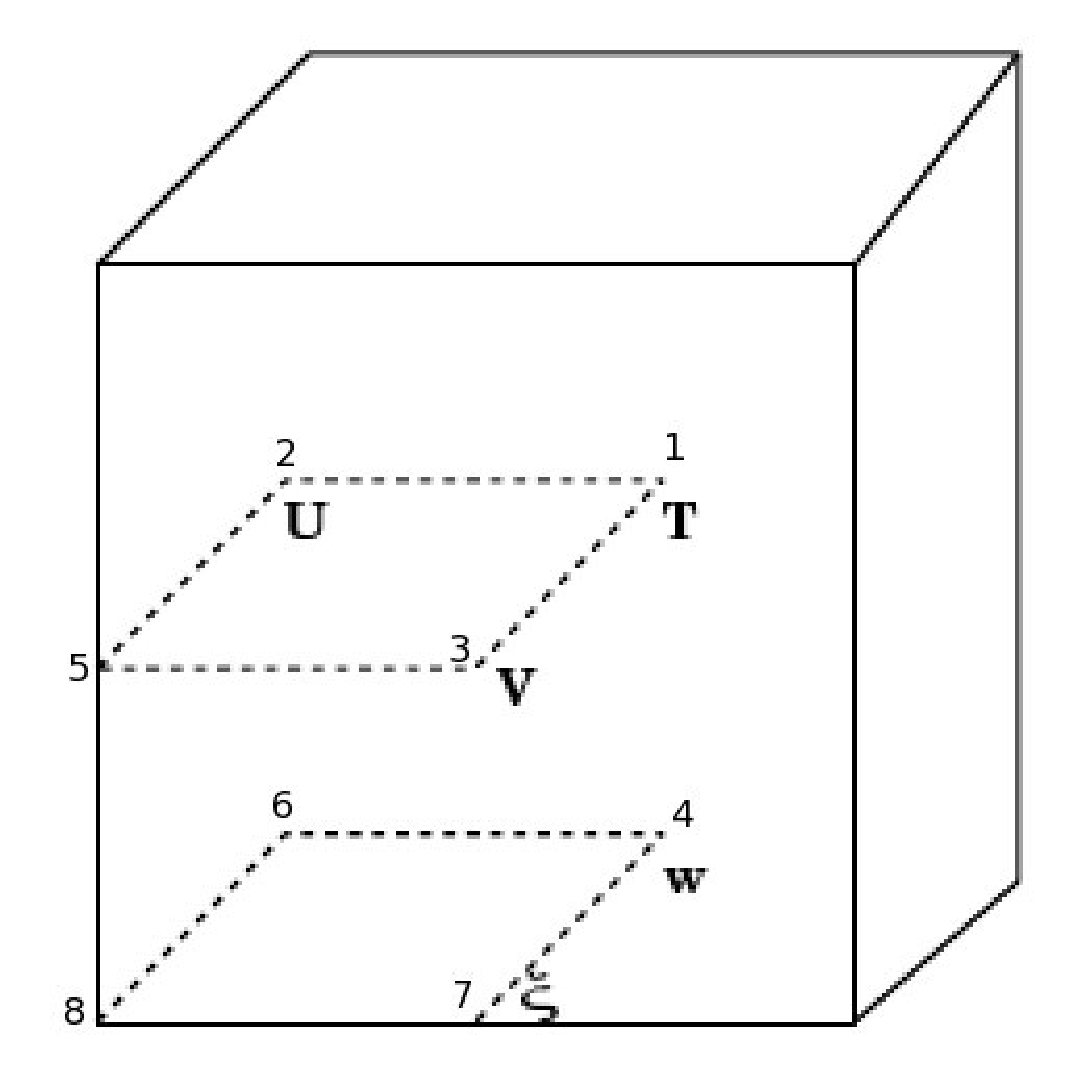
\includegraphics[width=8cm]{annexes/grilles}
\end{center}


\printindex
\phantomsection
\addcontentsline{toc}{chapter}{Index}
\end{document}
